\documentclass[twoside]{book}

% Packages required by doxygen
\usepackage{fixltx2e}
\usepackage{calc}
\usepackage{doxygen}
\usepackage[export]{adjustbox} % also loads graphicx
\usepackage{graphicx}
\usepackage[utf8]{inputenc}
\usepackage{makeidx}
\usepackage{multicol}
\usepackage{multirow}
\PassOptionsToPackage{warn}{textcomp}
\usepackage{textcomp}
\usepackage[nointegrals]{wasysym}
\usepackage[table]{xcolor}

% Font selection
\usepackage[T1]{fontenc}
\usepackage[scaled=.90]{helvet}
\usepackage{courier}
\usepackage{amssymb}
\usepackage{sectsty}
\renewcommand{\familydefault}{\sfdefault}
\allsectionsfont{%
  \fontseries{bc}\selectfont%
  \color{darkgray}%
}
\renewcommand{\DoxyLabelFont}{%
  \fontseries{bc}\selectfont%
  \color{darkgray}%
}
\newcommand{\+}{\discretionary{\mbox{\scriptsize$\hookleftarrow$}}{}{}}

% Page & text layout
\usepackage{geometry}
\geometry{%
  a4paper,%
  top=2.5cm,%
  bottom=2.5cm,%
  left=2.5cm,%
  right=2.5cm%
}
\tolerance=750
\hfuzz=15pt
\hbadness=750
\setlength{\emergencystretch}{15pt}
\setlength{\parindent}{0cm}
\setlength{\parskip}{3ex plus 2ex minus 2ex}
\makeatletter
\renewcommand{\paragraph}{%
  \@startsection{paragraph}{4}{0ex}{-1.0ex}{1.0ex}{%
    \normalfont\normalsize\bfseries\SS@parafont%
  }%
}
\renewcommand{\subparagraph}{%
  \@startsection{subparagraph}{5}{0ex}{-1.0ex}{1.0ex}{%
    \normalfont\normalsize\bfseries\SS@subparafont%
  }%
}
\makeatother

% Headers & footers
\usepackage{fancyhdr}
\pagestyle{fancyplain}
\fancyhead[LE]{\fancyplain{}{\bfseries\thepage}}
\fancyhead[CE]{\fancyplain{}{}}
\fancyhead[RE]{\fancyplain{}{\bfseries\leftmark}}
\fancyhead[LO]{\fancyplain{}{\bfseries\rightmark}}
\fancyhead[CO]{\fancyplain{}{}}
\fancyhead[RO]{\fancyplain{}{\bfseries\thepage}}
\fancyfoot[LE]{\fancyplain{}{}}
\fancyfoot[CE]{\fancyplain{}{}}
\fancyfoot[RE]{\fancyplain{}{\bfseries\scriptsize Generated by Doxygen }}
\fancyfoot[LO]{\fancyplain{}{\bfseries\scriptsize Generated by Doxygen }}
\fancyfoot[CO]{\fancyplain{}{}}
\fancyfoot[RO]{\fancyplain{}{}}
\renewcommand{\footrulewidth}{0.4pt}
\renewcommand{\chaptermark}[1]{%
  \markboth{#1}{}%
}
\renewcommand{\sectionmark}[1]{%
  \markright{\thesection\ #1}%
}

% Indices & bibliography
\usepackage{natbib}
\usepackage[titles]{tocloft}
\setcounter{tocdepth}{3}
\setcounter{secnumdepth}{5}
\makeindex

% Hyperlinks (required, but should be loaded last)
\usepackage{ifpdf}
\ifpdf
  \usepackage[pdftex,pagebackref=true]{hyperref}
\else
  \usepackage[ps2pdf,pagebackref=true]{hyperref}
\fi
\hypersetup{%
  colorlinks=true,%
  linkcolor=blue,%
  citecolor=blue,%
  unicode%
}

% Custom commands
\newcommand{\clearemptydoublepage}{%
  \newpage{\pagestyle{empty}\cleardoublepage}%
}

\usepackage{caption}
\captionsetup{labelsep=space,justification=centering,font={bf},singlelinecheck=off,skip=4pt,position=top}

%===== C O N T E N T S =====

\begin{document}

% Titlepage & ToC
\hypersetup{pageanchor=false,
             bookmarksnumbered=true,
             pdfencoding=unicode
            }
\pagenumbering{alph}
\begin{titlepage}
\vspace*{7cm}
\begin{center}%
{\Large Emploi du temps documentation }\\
\vspace*{1cm}
{\large Generated by Doxygen 1.8.12}\\
\end{center}
\end{titlepage}
\clearemptydoublepage
\pagenumbering{roman}
\tableofcontents
\clearemptydoublepage
\pagenumbering{arabic}
\hypersetup{pageanchor=true}

%--- Begin generated contents ---
\chapter{Namespace Index}
\section{Namespace List}
Here is a list of all namespaces with brief descriptions\+:\begin{DoxyCompactList}
\item\contentsline{section}{\hyperlink{namespace_catch}{Catch} }{\pageref{namespace_catch}}{}
\item\contentsline{section}{\hyperlink{namespace_catch_1_1_detail}{Catch\+::\+Detail} }{\pageref{namespace_catch_1_1_detail}}{}
\item\contentsline{section}{\hyperlink{namespace_catch_1_1_generators}{Catch\+::\+Generators} }{\pageref{namespace_catch_1_1_generators}}{}
\item\contentsline{section}{\hyperlink{namespace_catch_1_1_internal}{Catch\+::\+Internal} }{\pageref{namespace_catch_1_1_internal}}{}
\item\contentsline{section}{\hyperlink{namespace_catch_1_1_matchers}{Catch\+::\+Matchers} }{\pageref{namespace_catch_1_1_matchers}}{}
\item\contentsline{section}{\hyperlink{namespace_catch_1_1_matchers_1_1_impl}{Catch\+::\+Matchers\+::\+Impl} }{\pageref{namespace_catch_1_1_matchers_1_1_impl}}{}
\item\contentsline{section}{\hyperlink{namespace_catch_1_1_matchers_1_1_impl_1_1_generic}{Catch\+::\+Matchers\+::\+Impl\+::\+Generic} }{\pageref{namespace_catch_1_1_matchers_1_1_impl_1_1_generic}}{}
\item\contentsline{section}{\hyperlink{namespace_catch_1_1_matchers_1_1_impl_1_1_std_string}{Catch\+::\+Matchers\+::\+Impl\+::\+Std\+String} }{\pageref{namespace_catch_1_1_matchers_1_1_impl_1_1_std_string}}{}
\end{DoxyCompactList}

\chapter{Hierarchical Index}
\section{Class Hierarchy}
This inheritance list is sorted roughly, but not completely, alphabetically\+:\begin{DoxyCompactList}
\item \contentsline{section}{afficheur}{\pageref{classafficheur}}{}
\begin{DoxyCompactList}
\item \contentsline{section}{afficheur\+Console}{\pageref{classafficheur_console}}{}
\end{DoxyCompactList}
\item \contentsline{section}{Catch\+:\+:Detail\+:\+:Approx}{\pageref{class_catch_1_1_detail_1_1_approx}}{}
\item \contentsline{section}{Catch\+:\+:Assertion\+Info}{\pageref{struct_catch_1_1_assertion_info}}{}
\item \contentsline{section}{Catch\+:\+:Assertion\+Result}{\pageref{class_catch_1_1_assertion_result}}{}
\item \contentsline{section}{Catch\+:\+:Assertion\+Result\+Data}{\pageref{struct_catch_1_1_assertion_result_data}}{}
\item \contentsline{section}{Catch\+:\+:Auto\+Reg}{\pageref{struct_catch_1_1_auto_reg}}{}
\item \contentsline{section}{Catch\+:\+:Detail\+:\+:Borg\+Type}{\pageref{struct_catch_1_1_detail_1_1_borg_type}}{}
\item \contentsline{section}{Catch\+:\+:Matchers\+:\+:Impl\+:\+:Std\+String\+:\+:Cased\+String}{\pageref{struct_catch_1_1_matchers_1_1_impl_1_1_std_string_1_1_cased_string}}{}
\item \contentsline{section}{Catch\+:\+:Case\+Sensitive}{\pageref{struct_catch_1_1_case_sensitive}}{}
\item \contentsline{section}{Catch\+:\+:Composite\+Generator$<$ T $>$}{\pageref{class_catch_1_1_composite_generator}}{}
\item \contentsline{section}{Catch\+:\+:Copyable\+Stream}{\pageref{struct_catch_1_1_copyable_stream}}{}
\item \contentsline{section}{Catch\+:\+:Counts}{\pageref{struct_catch_1_1_counts}}{}
\item \contentsline{section}{cours}{\pageref{classcours}}{}
\item \contentsline{section}{Catch\+:\+:Internal\+:\+:Evaluator$<$ T1, T2, Op $>$}{\pageref{class_catch_1_1_internal_1_1_evaluator}}{}
\item \contentsline{section}{Catch\+:\+:Internal\+:\+:Evaluator$<$ T1, T2, Is\+Equal\+To $>$}{\pageref{struct_catch_1_1_internal_1_1_evaluator_3_01_t1_00_01_t2_00_01_is_equal_to_01_4}}{}
\item \contentsline{section}{Catch\+:\+:Internal\+:\+:Evaluator$<$ T1, T2, Is\+Greater\+Than $>$}{\pageref{struct_catch_1_1_internal_1_1_evaluator_3_01_t1_00_01_t2_00_01_is_greater_than_01_4}}{}
\item \contentsline{section}{Catch\+:\+:Internal\+:\+:Evaluator$<$ T1, T2, Is\+Greater\+Than\+Or\+Equal\+To $>$}{\pageref{struct_catch_1_1_internal_1_1_evaluator_3_01_t1_00_01_t2_00_01_is_greater_than_or_equal_to_01_4}}{}
\item \contentsline{section}{Catch\+:\+:Internal\+:\+:Evaluator$<$ T1, T2, Is\+Less\+Than $>$}{\pageref{struct_catch_1_1_internal_1_1_evaluator_3_01_t1_00_01_t2_00_01_is_less_than_01_4}}{}
\item \contentsline{section}{Catch\+:\+:Internal\+:\+:Evaluator$<$ T1, T2, Is\+Less\+Than\+Or\+Equal\+To $>$}{\pageref{struct_catch_1_1_internal_1_1_evaluator_3_01_t1_00_01_t2_00_01_is_less_than_or_equal_to_01_4}}{}
\item \contentsline{section}{Catch\+:\+:Internal\+:\+:Evaluator$<$ T1, T2, Is\+Not\+Equal\+To $>$}{\pageref{struct_catch_1_1_internal_1_1_evaluator_3_01_t1_00_01_t2_00_01_is_not_equal_to_01_4}}{}
\item exception\begin{DoxyCompactList}
\item \contentsline{section}{Catch\+:\+:Not\+Implemented\+Exception}{\pageref{class_catch_1_1_not_implemented_exception}}{}
\end{DoxyCompactList}
\item \contentsline{section}{Catch\+:\+:Exception\+Translator\+Registrar}{\pageref{class_catch_1_1_exception_translator_registrar}}{}
\item \contentsline{section}{Catch\+:\+:Expression\+Lhs$<$ T $>$}{\pageref{class_catch_1_1_expression_lhs}}{}
\item \contentsline{section}{Catch\+:\+:Detail\+:\+:False\+Type}{\pageref{struct_catch_1_1_detail_1_1_false_type}}{}
\item \contentsline{section}{horaire}{\pageref{classhoraire}}{}
\item \contentsline{section}{Catch\+:\+:I\+Context}{\pageref{struct_catch_1_1_i_context}}{}
\begin{DoxyCompactList}
\item \contentsline{section}{Catch\+:\+:I\+Mutable\+Context}{\pageref{struct_catch_1_1_i_mutable_context}}{}
\end{DoxyCompactList}
\item \contentsline{section}{Catch\+:\+:I\+Exception\+Translator}{\pageref{struct_catch_1_1_i_exception_translator}}{}
\item \contentsline{section}{Catch\+:\+:I\+Exception\+Translator\+Registry}{\pageref{struct_catch_1_1_i_exception_translator_registry}}{}
\item \contentsline{section}{Catch\+:\+:I\+Generator$<$ T $>$}{\pageref{struct_catch_1_1_i_generator}}{}
\begin{DoxyCompactList}
\item \contentsline{section}{Catch\+:\+:Between\+Generator$<$ T $>$}{\pageref{class_catch_1_1_between_generator}}{}
\item \contentsline{section}{Catch\+:\+:Values\+Generator$<$ T $>$}{\pageref{class_catch_1_1_values_generator}}{}
\end{DoxyCompactList}
\item \contentsline{section}{Catch\+:\+:I\+Generator\+Info}{\pageref{struct_catch_1_1_i_generator_info}}{}
\item \contentsline{section}{Catch\+:\+:I\+Generators\+For\+Test}{\pageref{struct_catch_1_1_i_generators_for_test}}{}
\item \contentsline{section}{Catch\+:\+:I\+Mutable\+Registry\+Hub}{\pageref{struct_catch_1_1_i_mutable_registry_hub}}{}
\item \contentsline{section}{Catch\+:\+:I\+Registry\+Hub}{\pageref{struct_catch_1_1_i_registry_hub}}{}
\item \contentsline{section}{Catch\+:\+:I\+Result\+Capture}{\pageref{struct_catch_1_1_i_result_capture}}{}
\item \contentsline{section}{Catch\+:\+:I\+Runner}{\pageref{struct_catch_1_1_i_runner}}{}
\item \contentsline{section}{Catch\+:\+:Detail\+:\+:Is\+Stream\+Insertable$<$ T $>$}{\pageref{struct_catch_1_1_detail_1_1_is_stream_insertable}}{}
\item \contentsline{section}{Catch\+:\+:I\+Tag\+Alias\+Registry}{\pageref{struct_catch_1_1_i_tag_alias_registry}}{}
\item \contentsline{section}{Catch\+:\+:I\+Test\+Case\+Registry}{\pageref{struct_catch_1_1_i_test_case_registry}}{}
\item \contentsline{section}{liste\+Cours}{\pageref{classliste_cours}}{}
\item \contentsline{section}{liste\+D\+Horaire}{\pageref{classliste_d_horaire}}{}
\item \contentsline{section}{liste\+Ressources}{\pageref{classliste_ressources}}{}
\item \contentsline{section}{Catch\+:\+:Message\+Builder}{\pageref{struct_catch_1_1_message_builder}}{}
\item \contentsline{section}{Catch\+:\+:Message\+Info}{\pageref{struct_catch_1_1_message_info}}{}
\item \contentsline{section}{Catch\+:\+:Name\+And\+Desc}{\pageref{struct_catch_1_1_name_and_desc}}{}
\item \contentsline{section}{Catch\+:\+:Non\+Copyable}{\pageref{class_catch_1_1_non_copyable}}{}
\begin{DoxyCompactList}
\item \contentsline{section}{Catch\+:\+:I\+Shared}{\pageref{struct_catch_1_1_i_shared}}{}
\begin{DoxyCompactList}
\item \contentsline{section}{Catch\+:\+:I\+Test\+Case}{\pageref{struct_catch_1_1_i_test_case}}{}
\begin{DoxyCompactList}
\item \contentsline{section}{Catch\+:\+:Shared\+Impl$<$ I\+Test\+Case $>$}{\pageref{struct_catch_1_1_shared_impl}}{}
\begin{DoxyCompactList}
\item \contentsline{section}{Catch\+:\+:Method\+Test\+Case$<$ C $>$}{\pageref{class_catch_1_1_method_test_case}}{}
\end{DoxyCompactList}
\end{DoxyCompactList}
\item \contentsline{section}{Catch\+:\+:Shared\+Impl$<$ I\+Shared $>$}{\pageref{struct_catch_1_1_shared_impl}}{}
\begin{DoxyCompactList}
\item \contentsline{section}{Catch\+:\+:Matchers\+:\+:Impl\+:\+:Matcher$<$ ExpressionT $>$}{\pageref{struct_catch_1_1_matchers_1_1_impl_1_1_matcher}}{}
\begin{DoxyCompactList}
\item \contentsline{section}{Catch\+:\+:Matchers\+:\+:Impl\+:\+:Matcher\+Impl$<$ DerivedT, ExpressionT $>$}{\pageref{struct_catch_1_1_matchers_1_1_impl_1_1_matcher_impl}}{}
\item \contentsline{section}{Catch\+:\+:Matchers\+:\+:Impl\+:\+:Matcher\+Impl$<$ All\+Of$<$ ExpressionT $>$, ExpressionT $>$}{\pageref{struct_catch_1_1_matchers_1_1_impl_1_1_matcher_impl}}{}
\begin{DoxyCompactList}
\item \contentsline{section}{Catch\+:\+:Matchers\+:\+:Impl\+:\+:Generic\+:\+:All\+Of$<$ ExpressionT $>$}{\pageref{class_catch_1_1_matchers_1_1_impl_1_1_generic_1_1_all_of}}{}
\end{DoxyCompactList}
\item \contentsline{section}{Catch\+:\+:Matchers\+:\+:Impl\+:\+:Matcher\+Impl$<$ Any\+Of$<$ ExpressionT $>$, ExpressionT $>$}{\pageref{struct_catch_1_1_matchers_1_1_impl_1_1_matcher_impl}}{}
\begin{DoxyCompactList}
\item \contentsline{section}{Catch\+:\+:Matchers\+:\+:Impl\+:\+:Generic\+:\+:Any\+Of$<$ ExpressionT $>$}{\pageref{class_catch_1_1_matchers_1_1_impl_1_1_generic_1_1_any_of}}{}
\end{DoxyCompactList}
\item \contentsline{section}{Catch\+:\+:Matchers\+:\+:Impl\+:\+:Matcher\+Impl$<$ Not$<$ ExpressionT $>$, ExpressionT $>$}{\pageref{struct_catch_1_1_matchers_1_1_impl_1_1_matcher_impl}}{}
\begin{DoxyCompactList}
\item \contentsline{section}{Catch\+:\+:Matchers\+:\+:Impl\+:\+:Generic\+:\+:Not$<$ ExpressionT $>$}{\pageref{class_catch_1_1_matchers_1_1_impl_1_1_generic_1_1_not}}{}
\end{DoxyCompactList}
\end{DoxyCompactList}
\item \contentsline{section}{Catch\+:\+:Matchers\+:\+:Impl\+:\+:Matcher$<$ std\+:\+:string $>$}{\pageref{struct_catch_1_1_matchers_1_1_impl_1_1_matcher}}{}
\begin{DoxyCompactList}
\item \contentsline{section}{Catch\+:\+:Matchers\+:\+:Impl\+:\+:Matcher\+Impl$<$ Contains, std\+:\+:string $>$}{\pageref{struct_catch_1_1_matchers_1_1_impl_1_1_matcher_impl}}{}
\begin{DoxyCompactList}
\item \contentsline{section}{Catch\+:\+:Matchers\+:\+:Impl\+:\+:Std\+String\+:\+:Contains}{\pageref{struct_catch_1_1_matchers_1_1_impl_1_1_std_string_1_1_contains}}{}
\end{DoxyCompactList}
\item \contentsline{section}{Catch\+:\+:Matchers\+:\+:Impl\+:\+:Matcher\+Impl$<$ Ends\+With, std\+:\+:string $>$}{\pageref{struct_catch_1_1_matchers_1_1_impl_1_1_matcher_impl}}{}
\begin{DoxyCompactList}
\item \contentsline{section}{Catch\+:\+:Matchers\+:\+:Impl\+:\+:Std\+String\+:\+:Ends\+With}{\pageref{struct_catch_1_1_matchers_1_1_impl_1_1_std_string_1_1_ends_with}}{}
\end{DoxyCompactList}
\item \contentsline{section}{Catch\+:\+:Matchers\+:\+:Impl\+:\+:Matcher\+Impl$<$ Equals, std\+:\+:string $>$}{\pageref{struct_catch_1_1_matchers_1_1_impl_1_1_matcher_impl}}{}
\begin{DoxyCompactList}
\item \contentsline{section}{Catch\+:\+:Matchers\+:\+:Impl\+:\+:Std\+String\+:\+:Equals}{\pageref{struct_catch_1_1_matchers_1_1_impl_1_1_std_string_1_1_equals}}{}
\end{DoxyCompactList}
\item \contentsline{section}{Catch\+:\+:Matchers\+:\+:Impl\+:\+:Matcher\+Impl$<$ Starts\+With, std\+:\+:string $>$}{\pageref{struct_catch_1_1_matchers_1_1_impl_1_1_matcher_impl}}{}
\begin{DoxyCompactList}
\item \contentsline{section}{Catch\+:\+:Matchers\+:\+:Impl\+:\+:Std\+String\+:\+:Starts\+With}{\pageref{struct_catch_1_1_matchers_1_1_impl_1_1_std_string_1_1_starts_with}}{}
\end{DoxyCompactList}
\end{DoxyCompactList}
\end{DoxyCompactList}
\end{DoxyCompactList}
\item \contentsline{section}{Catch\+:\+:Section}{\pageref{class_catch_1_1_section}}{}
\end{DoxyCompactList}
\item \contentsline{section}{Catch\+:\+:Internal\+:\+:Operator\+Traits$<$ Op $>$}{\pageref{struct_catch_1_1_internal_1_1_operator_traits}}{}
\item \contentsline{section}{Catch\+:\+:Internal\+:\+:Operator\+Traits$<$ Is\+Equal\+To $>$}{\pageref{struct_catch_1_1_internal_1_1_operator_traits_3_01_is_equal_to_01_4}}{}
\item \contentsline{section}{Catch\+:\+:Internal\+:\+:Operator\+Traits$<$ Is\+Greater\+Than $>$}{\pageref{struct_catch_1_1_internal_1_1_operator_traits_3_01_is_greater_than_01_4}}{}
\item \contentsline{section}{Catch\+:\+:Internal\+:\+:Operator\+Traits$<$ Is\+Greater\+Than\+Or\+Equal\+To $>$}{\pageref{struct_catch_1_1_internal_1_1_operator_traits_3_01_is_greater_than_or_equal_to_01_4}}{}
\item \contentsline{section}{Catch\+:\+:Internal\+:\+:Operator\+Traits$<$ Is\+Less\+Than $>$}{\pageref{struct_catch_1_1_internal_1_1_operator_traits_3_01_is_less_than_01_4}}{}
\item \contentsline{section}{Catch\+:\+:Internal\+:\+:Operator\+Traits$<$ Is\+Less\+Than\+Or\+Equal\+To $>$}{\pageref{struct_catch_1_1_internal_1_1_operator_traits_3_01_is_less_than_or_equal_to_01_4}}{}
\item \contentsline{section}{Catch\+:\+:Internal\+:\+:Operator\+Traits$<$ Is\+Not\+Equal\+To $>$}{\pageref{struct_catch_1_1_internal_1_1_operator_traits_3_01_is_not_equal_to_01_4}}{}
\item \contentsline{section}{Catch\+:\+:Option$<$ T $>$}{\pageref{class_catch_1_1_option}}{}
\item \contentsline{section}{Catch\+:\+:pluralise}{\pageref{struct_catch_1_1pluralise}}{}
\item \contentsline{section}{Catch\+:\+:Ptr$<$ T $>$}{\pageref{class_catch_1_1_ptr}}{}
\item \contentsline{section}{Catch\+:\+:Ptr$<$ Catch\+:\+:I\+Test\+Case $>$}{\pageref{class_catch_1_1_ptr}}{}
\item \contentsline{section}{Catch\+:\+:Ptr$<$ Catch\+:\+:Matchers\+:\+:Impl\+:\+:Matcher$<$ ExpressionT $>$ $>$}{\pageref{class_catch_1_1_ptr}}{}
\item \contentsline{section}{Catch\+:\+:Registrar\+For\+Tag\+Aliases}{\pageref{struct_catch_1_1_registrar_for_tag_aliases}}{}
\item \contentsline{section}{ressource}{\pageref{classressource}}{}
\begin{DoxyCompactList}
\item \contentsline{section}{formation}{\pageref{classformation}}{}
\item \contentsline{section}{professeur}{\pageref{classprofesseur}}{}
\end{DoxyCompactList}
\item \contentsline{section}{Catch\+:\+:Result\+Builder}{\pageref{class_catch_1_1_result_builder}}{}
\item \contentsline{section}{Catch\+:\+:Result\+Disposition}{\pageref{struct_catch_1_1_result_disposition}}{}
\item \contentsline{section}{Catch\+:\+:Result\+Was}{\pageref{struct_catch_1_1_result_was}}{}
\item \contentsline{section}{Catch\+:\+:Safe\+Bool}{\pageref{class_catch_1_1_safe_bool}}{}
\item \contentsline{section}{salle}{\pageref{classsalle}}{}
\item \contentsline{section}{Catch\+:\+:Scoped\+Message}{\pageref{class_catch_1_1_scoped_message}}{}
\item \contentsline{section}{Catch\+:\+:Section\+End\+Info}{\pageref{struct_catch_1_1_section_end_info}}{}
\item \contentsline{section}{Catch\+:\+:Section\+Info}{\pageref{struct_catch_1_1_section_info}}{}
\item \contentsline{section}{Catch\+:\+:Source\+Line\+Info}{\pageref{struct_catch_1_1_source_line_info}}{}
\item \contentsline{section}{Catch\+:\+:Stream\+End\+Stop}{\pageref{struct_catch_1_1_stream_end_stop}}{}
\item \contentsline{section}{Catch\+:\+:String\+Maker$<$ R C\+:\+:$\ast$ $>$}{\pageref{struct_catch_1_1_string_maker_3_01_r_01_c_1_1_5_01_4}}{}
\item \contentsline{section}{Catch\+:\+:String\+Maker$<$ T $\ast$ $>$}{\pageref{struct_catch_1_1_string_maker_3_01_t_01_5_01_4}}{}
\item \contentsline{section}{Catch\+:\+:Detail\+:\+:String\+Maker\+Base$<$ C $>$}{\pageref{struct_catch_1_1_detail_1_1_string_maker_base}}{}
\item \contentsline{section}{Catch\+:\+:Detail\+:\+:String\+Maker\+Base$<$ Detail\+:\+:Is\+Stream\+Insertable$<$ T $>$\+:\+:value $>$}{\pageref{struct_catch_1_1_detail_1_1_string_maker_base}}{}
\begin{DoxyCompactList}
\item \contentsline{section}{Catch\+:\+:String\+Maker$<$ T $>$}{\pageref{struct_catch_1_1_string_maker}}{}
\end{DoxyCompactList}
\item \contentsline{section}{Catch\+:\+:Detail\+:\+:String\+Maker\+Base$<$ true $>$}{\pageref{struct_catch_1_1_detail_1_1_string_maker_base_3_01true_01_4}}{}
\item \contentsline{section}{Catch\+:\+:Tag\+Alias}{\pageref{struct_catch_1_1_tag_alias}}{}
\item \contentsline{section}{Catch\+:\+:Test\+Case\+Info}{\pageref{struct_catch_1_1_test_case_info}}{}
\begin{DoxyCompactList}
\item \contentsline{section}{Catch\+:\+:Test\+Case}{\pageref{class_catch_1_1_test_case}}{}
\end{DoxyCompactList}
\item \contentsline{section}{Catch\+:\+:Test\+Failure\+Exception}{\pageref{struct_catch_1_1_test_failure_exception}}{}
\item \contentsline{section}{Catch\+:\+:Timer}{\pageref{class_catch_1_1_timer}}{}
\item \contentsline{section}{Catch\+:\+:Totals}{\pageref{struct_catch_1_1_totals}}{}
\item \contentsline{section}{Catch\+:\+:Detail\+:\+:True\+Type}{\pageref{struct_catch_1_1_detail_1_1_true_type}}{}
\item T\begin{DoxyCompactList}
\item \contentsline{section}{Catch\+:\+:Shared\+Impl$<$ T $>$}{\pageref{struct_catch_1_1_shared_impl}}{}
\end{DoxyCompactList}
\end{DoxyCompactList}

\chapter{Class Index}
\section{Class List}
Here are the classes, structs, unions and interfaces with brief descriptions\+:\begin{DoxyCompactList}
\item\contentsline{section}{\hyperlink{classafficheur_console}{afficheur\+Console} }{\pageref{classafficheur_console}}{}
\item\contentsline{section}{\hyperlink{class_catch_1_1_matchers_1_1_impl_1_1_generic_1_1_all_of}{Catch\+::\+Matchers\+::\+Impl\+::\+Generic\+::\+All\+Of$<$ Expression\+T $>$} }{\pageref{class_catch_1_1_matchers_1_1_impl_1_1_generic_1_1_all_of}}{}
\item\contentsline{section}{\hyperlink{class_catch_1_1_matchers_1_1_impl_1_1_generic_1_1_any_of}{Catch\+::\+Matchers\+::\+Impl\+::\+Generic\+::\+Any\+Of$<$ Expression\+T $>$} }{\pageref{class_catch_1_1_matchers_1_1_impl_1_1_generic_1_1_any_of}}{}
\item\contentsline{section}{\hyperlink{class_catch_1_1_detail_1_1_approx}{Catch\+::\+Detail\+::\+Approx} }{\pageref{class_catch_1_1_detail_1_1_approx}}{}
\item\contentsline{section}{\hyperlink{struct_catch_1_1_assertion_info}{Catch\+::\+Assertion\+Info} }{\pageref{struct_catch_1_1_assertion_info}}{}
\item\contentsline{section}{\hyperlink{class_catch_1_1_assertion_result}{Catch\+::\+Assertion\+Result} }{\pageref{class_catch_1_1_assertion_result}}{}
\item\contentsline{section}{\hyperlink{struct_catch_1_1_assertion_result_data}{Catch\+::\+Assertion\+Result\+Data} }{\pageref{struct_catch_1_1_assertion_result_data}}{}
\item\contentsline{section}{\hyperlink{struct_catch_1_1_auto_reg}{Catch\+::\+Auto\+Reg} }{\pageref{struct_catch_1_1_auto_reg}}{}
\item\contentsline{section}{\hyperlink{class_catch_1_1_between_generator}{Catch\+::\+Between\+Generator$<$ T $>$} }{\pageref{class_catch_1_1_between_generator}}{}
\item\contentsline{section}{\hyperlink{struct_catch_1_1_detail_1_1_borg_type}{Catch\+::\+Detail\+::\+Borg\+Type} }{\pageref{struct_catch_1_1_detail_1_1_borg_type}}{}
\item\contentsline{section}{\hyperlink{struct_catch_1_1_matchers_1_1_impl_1_1_std_string_1_1_cased_string}{Catch\+::\+Matchers\+::\+Impl\+::\+Std\+String\+::\+Cased\+String} }{\pageref{struct_catch_1_1_matchers_1_1_impl_1_1_std_string_1_1_cased_string}}{}
\item\contentsline{section}{\hyperlink{struct_catch_1_1_case_sensitive}{Catch\+::\+Case\+Sensitive} }{\pageref{struct_catch_1_1_case_sensitive}}{}
\item\contentsline{section}{\hyperlink{class_catch_1_1_composite_generator}{Catch\+::\+Composite\+Generator$<$ T $>$} }{\pageref{class_catch_1_1_composite_generator}}{}
\item\contentsline{section}{\hyperlink{struct_catch_1_1_matchers_1_1_impl_1_1_std_string_1_1_contains}{Catch\+::\+Matchers\+::\+Impl\+::\+Std\+String\+::\+Contains} }{\pageref{struct_catch_1_1_matchers_1_1_impl_1_1_std_string_1_1_contains}}{}
\item\contentsline{section}{\hyperlink{struct_catch_1_1_copyable_stream}{Catch\+::\+Copyable\+Stream} }{\pageref{struct_catch_1_1_copyable_stream}}{}
\item\contentsline{section}{\hyperlink{struct_catch_1_1_counts}{Catch\+::\+Counts} }{\pageref{struct_catch_1_1_counts}}{}
\item\contentsline{section}{\hyperlink{classcours}{cours} }{\pageref{classcours}}{}
\item\contentsline{section}{\hyperlink{struct_catch_1_1_matchers_1_1_impl_1_1_std_string_1_1_ends_with}{Catch\+::\+Matchers\+::\+Impl\+::\+Std\+String\+::\+Ends\+With} }{\pageref{struct_catch_1_1_matchers_1_1_impl_1_1_std_string_1_1_ends_with}}{}
\item\contentsline{section}{\hyperlink{struct_catch_1_1_matchers_1_1_impl_1_1_std_string_1_1_equals}{Catch\+::\+Matchers\+::\+Impl\+::\+Std\+String\+::\+Equals} }{\pageref{struct_catch_1_1_matchers_1_1_impl_1_1_std_string_1_1_equals}}{}
\item\contentsline{section}{\hyperlink{class_catch_1_1_internal_1_1_evaluator}{Catch\+::\+Internal\+::\+Evaluator$<$ T1, T2, Op $>$} }{\pageref{class_catch_1_1_internal_1_1_evaluator}}{}
\item\contentsline{section}{\hyperlink{struct_catch_1_1_internal_1_1_evaluator_3_01_t1_00_01_t2_00_01_is_equal_to_01_4}{Catch\+::\+Internal\+::\+Evaluator$<$ T1, T2, Is\+Equal\+To $>$} }{\pageref{struct_catch_1_1_internal_1_1_evaluator_3_01_t1_00_01_t2_00_01_is_equal_to_01_4}}{}
\item\contentsline{section}{\hyperlink{struct_catch_1_1_internal_1_1_evaluator_3_01_t1_00_01_t2_00_01_is_greater_than_01_4}{Catch\+::\+Internal\+::\+Evaluator$<$ T1, T2, Is\+Greater\+Than $>$} }{\pageref{struct_catch_1_1_internal_1_1_evaluator_3_01_t1_00_01_t2_00_01_is_greater_than_01_4}}{}
\item\contentsline{section}{\hyperlink{struct_catch_1_1_internal_1_1_evaluator_3_01_t1_00_01_t2_00_01_is_greater_than_or_equal_to_01_4}{Catch\+::\+Internal\+::\+Evaluator$<$ T1, T2, Is\+Greater\+Than\+Or\+Equal\+To $>$} }{\pageref{struct_catch_1_1_internal_1_1_evaluator_3_01_t1_00_01_t2_00_01_is_greater_than_or_equal_to_01_4}}{}
\item\contentsline{section}{\hyperlink{struct_catch_1_1_internal_1_1_evaluator_3_01_t1_00_01_t2_00_01_is_less_than_01_4}{Catch\+::\+Internal\+::\+Evaluator$<$ T1, T2, Is\+Less\+Than $>$} }{\pageref{struct_catch_1_1_internal_1_1_evaluator_3_01_t1_00_01_t2_00_01_is_less_than_01_4}}{}
\item\contentsline{section}{\hyperlink{struct_catch_1_1_internal_1_1_evaluator_3_01_t1_00_01_t2_00_01_is_less_than_or_equal_to_01_4}{Catch\+::\+Internal\+::\+Evaluator$<$ T1, T2, Is\+Less\+Than\+Or\+Equal\+To $>$} }{\pageref{struct_catch_1_1_internal_1_1_evaluator_3_01_t1_00_01_t2_00_01_is_less_than_or_equal_to_01_4}}{}
\item\contentsline{section}{\hyperlink{struct_catch_1_1_internal_1_1_evaluator_3_01_t1_00_01_t2_00_01_is_not_equal_to_01_4}{Catch\+::\+Internal\+::\+Evaluator$<$ T1, T2, Is\+Not\+Equal\+To $>$} }{\pageref{struct_catch_1_1_internal_1_1_evaluator_3_01_t1_00_01_t2_00_01_is_not_equal_to_01_4}}{}
\item\contentsline{section}{\hyperlink{class_catch_1_1_exception_translator_registrar}{Catch\+::\+Exception\+Translator\+Registrar} }{\pageref{class_catch_1_1_exception_translator_registrar}}{}
\item\contentsline{section}{\hyperlink{class_catch_1_1_expression_lhs}{Catch\+::\+Expression\+Lhs$<$ T $>$} }{\pageref{class_catch_1_1_expression_lhs}}{}
\item\contentsline{section}{\hyperlink{struct_catch_1_1_detail_1_1_false_type}{Catch\+::\+Detail\+::\+False\+Type} }{\pageref{struct_catch_1_1_detail_1_1_false_type}}{}
\item\contentsline{section}{\hyperlink{classformation}{formation} }{\pageref{classformation}}{}
\item\contentsline{section}{\hyperlink{classhoraire}{horaire} }{\pageref{classhoraire}}{}
\item\contentsline{section}{\hyperlink{struct_catch_1_1_i_context}{Catch\+::\+I\+Context} }{\pageref{struct_catch_1_1_i_context}}{}
\item\contentsline{section}{\hyperlink{struct_catch_1_1_i_exception_translator}{Catch\+::\+I\+Exception\+Translator} }{\pageref{struct_catch_1_1_i_exception_translator}}{}
\item\contentsline{section}{\hyperlink{struct_catch_1_1_i_exception_translator_registry}{Catch\+::\+I\+Exception\+Translator\+Registry} }{\pageref{struct_catch_1_1_i_exception_translator_registry}}{}
\item\contentsline{section}{\hyperlink{struct_catch_1_1_i_generator}{Catch\+::\+I\+Generator$<$ T $>$} }{\pageref{struct_catch_1_1_i_generator}}{}
\item\contentsline{section}{\hyperlink{struct_catch_1_1_i_generator_info}{Catch\+::\+I\+Generator\+Info} }{\pageref{struct_catch_1_1_i_generator_info}}{}
\item\contentsline{section}{\hyperlink{struct_catch_1_1_i_generators_for_test}{Catch\+::\+I\+Generators\+For\+Test} }{\pageref{struct_catch_1_1_i_generators_for_test}}{}
\item\contentsline{section}{\hyperlink{struct_catch_1_1_i_mutable_context}{Catch\+::\+I\+Mutable\+Context} }{\pageref{struct_catch_1_1_i_mutable_context}}{}
\item\contentsline{section}{\hyperlink{struct_catch_1_1_i_mutable_registry_hub}{Catch\+::\+I\+Mutable\+Registry\+Hub} }{\pageref{struct_catch_1_1_i_mutable_registry_hub}}{}
\item\contentsline{section}{\hyperlink{struct_catch_1_1_i_registry_hub}{Catch\+::\+I\+Registry\+Hub} }{\pageref{struct_catch_1_1_i_registry_hub}}{}
\item\contentsline{section}{\hyperlink{struct_catch_1_1_i_result_capture}{Catch\+::\+I\+Result\+Capture} }{\pageref{struct_catch_1_1_i_result_capture}}{}
\item\contentsline{section}{\hyperlink{struct_catch_1_1_i_runner}{Catch\+::\+I\+Runner} }{\pageref{struct_catch_1_1_i_runner}}{}
\item\contentsline{section}{\hyperlink{struct_catch_1_1_i_shared}{Catch\+::\+I\+Shared} }{\pageref{struct_catch_1_1_i_shared}}{}
\item\contentsline{section}{\hyperlink{struct_catch_1_1_detail_1_1_is_stream_insertable}{Catch\+::\+Detail\+::\+Is\+Stream\+Insertable$<$ T $>$} }{\pageref{struct_catch_1_1_detail_1_1_is_stream_insertable}}{}
\item\contentsline{section}{\hyperlink{struct_catch_1_1_i_tag_alias_registry}{Catch\+::\+I\+Tag\+Alias\+Registry} }{\pageref{struct_catch_1_1_i_tag_alias_registry}}{}
\item\contentsline{section}{\hyperlink{struct_catch_1_1_i_test_case}{Catch\+::\+I\+Test\+Case} }{\pageref{struct_catch_1_1_i_test_case}}{}
\item\contentsline{section}{\hyperlink{struct_catch_1_1_i_test_case_registry}{Catch\+::\+I\+Test\+Case\+Registry} }{\pageref{struct_catch_1_1_i_test_case_registry}}{}
\item\contentsline{section}{\hyperlink{classliste_cours}{liste\+Cours} }{\pageref{classliste_cours}}{}
\item\contentsline{section}{\hyperlink{classliste_d_horaire}{liste\+D\+Horaire} }{\pageref{classliste_d_horaire}}{}
\item\contentsline{section}{\hyperlink{classliste_ressources}{liste\+Ressources} }{\pageref{classliste_ressources}}{}
\item\contentsline{section}{\hyperlink{struct_catch_1_1_matchers_1_1_impl_1_1_matcher}{Catch\+::\+Matchers\+::\+Impl\+::\+Matcher$<$ Expression\+T $>$} }{\pageref{struct_catch_1_1_matchers_1_1_impl_1_1_matcher}}{}
\item\contentsline{section}{\hyperlink{struct_catch_1_1_matchers_1_1_impl_1_1_matcher_impl}{Catch\+::\+Matchers\+::\+Impl\+::\+Matcher\+Impl$<$ Derived\+T, Expression\+T $>$} }{\pageref{struct_catch_1_1_matchers_1_1_impl_1_1_matcher_impl}}{}
\item\contentsline{section}{\hyperlink{struct_catch_1_1_message_builder}{Catch\+::\+Message\+Builder} }{\pageref{struct_catch_1_1_message_builder}}{}
\item\contentsline{section}{\hyperlink{struct_catch_1_1_message_info}{Catch\+::\+Message\+Info} }{\pageref{struct_catch_1_1_message_info}}{}
\item\contentsline{section}{\hyperlink{class_catch_1_1_method_test_case}{Catch\+::\+Method\+Test\+Case$<$ C $>$} }{\pageref{class_catch_1_1_method_test_case}}{}
\item\contentsline{section}{\hyperlink{struct_catch_1_1_name_and_desc}{Catch\+::\+Name\+And\+Desc} }{\pageref{struct_catch_1_1_name_and_desc}}{}
\item\contentsline{section}{\hyperlink{class_catch_1_1_non_copyable}{Catch\+::\+Non\+Copyable} }{\pageref{class_catch_1_1_non_copyable}}{}
\item\contentsline{section}{\hyperlink{class_catch_1_1_matchers_1_1_impl_1_1_generic_1_1_not}{Catch\+::\+Matchers\+::\+Impl\+::\+Generic\+::\+Not$<$ Expression\+T $>$} }{\pageref{class_catch_1_1_matchers_1_1_impl_1_1_generic_1_1_not}}{}
\item\contentsline{section}{\hyperlink{class_catch_1_1_not_implemented_exception}{Catch\+::\+Not\+Implemented\+Exception} }{\pageref{class_catch_1_1_not_implemented_exception}}{}
\item\contentsline{section}{\hyperlink{struct_catch_1_1_internal_1_1_operator_traits}{Catch\+::\+Internal\+::\+Operator\+Traits$<$ Op $>$} }{\pageref{struct_catch_1_1_internal_1_1_operator_traits}}{}
\item\contentsline{section}{\hyperlink{struct_catch_1_1_internal_1_1_operator_traits_3_01_is_equal_to_01_4}{Catch\+::\+Internal\+::\+Operator\+Traits$<$ Is\+Equal\+To $>$} }{\pageref{struct_catch_1_1_internal_1_1_operator_traits_3_01_is_equal_to_01_4}}{}
\item\contentsline{section}{\hyperlink{struct_catch_1_1_internal_1_1_operator_traits_3_01_is_greater_than_01_4}{Catch\+::\+Internal\+::\+Operator\+Traits$<$ Is\+Greater\+Than $>$} }{\pageref{struct_catch_1_1_internal_1_1_operator_traits_3_01_is_greater_than_01_4}}{}
\item\contentsline{section}{\hyperlink{struct_catch_1_1_internal_1_1_operator_traits_3_01_is_greater_than_or_equal_to_01_4}{Catch\+::\+Internal\+::\+Operator\+Traits$<$ Is\+Greater\+Than\+Or\+Equal\+To $>$} }{\pageref{struct_catch_1_1_internal_1_1_operator_traits_3_01_is_greater_than_or_equal_to_01_4}}{}
\item\contentsline{section}{\hyperlink{struct_catch_1_1_internal_1_1_operator_traits_3_01_is_less_than_01_4}{Catch\+::\+Internal\+::\+Operator\+Traits$<$ Is\+Less\+Than $>$} }{\pageref{struct_catch_1_1_internal_1_1_operator_traits_3_01_is_less_than_01_4}}{}
\item\contentsline{section}{\hyperlink{struct_catch_1_1_internal_1_1_operator_traits_3_01_is_less_than_or_equal_to_01_4}{Catch\+::\+Internal\+::\+Operator\+Traits$<$ Is\+Less\+Than\+Or\+Equal\+To $>$} }{\pageref{struct_catch_1_1_internal_1_1_operator_traits_3_01_is_less_than_or_equal_to_01_4}}{}
\item\contentsline{section}{\hyperlink{struct_catch_1_1_internal_1_1_operator_traits_3_01_is_not_equal_to_01_4}{Catch\+::\+Internal\+::\+Operator\+Traits$<$ Is\+Not\+Equal\+To $>$} }{\pageref{struct_catch_1_1_internal_1_1_operator_traits_3_01_is_not_equal_to_01_4}}{}
\item\contentsline{section}{\hyperlink{class_catch_1_1_option}{Catch\+::\+Option$<$ T $>$} }{\pageref{class_catch_1_1_option}}{}
\item\contentsline{section}{\hyperlink{struct_catch_1_1pluralise}{Catch\+::pluralise} }{\pageref{struct_catch_1_1pluralise}}{}
\item\contentsline{section}{\hyperlink{classprofesseur}{professeur} }{\pageref{classprofesseur}}{}
\item\contentsline{section}{\hyperlink{class_catch_1_1_ptr}{Catch\+::\+Ptr$<$ T $>$} }{\pageref{class_catch_1_1_ptr}}{}
\item\contentsline{section}{\hyperlink{struct_catch_1_1_registrar_for_tag_aliases}{Catch\+::\+Registrar\+For\+Tag\+Aliases} }{\pageref{struct_catch_1_1_registrar_for_tag_aliases}}{}
\item\contentsline{section}{\hyperlink{classressource}{ressource} }{\pageref{classressource}}{}
\item\contentsline{section}{\hyperlink{class_catch_1_1_result_builder}{Catch\+::\+Result\+Builder} }{\pageref{class_catch_1_1_result_builder}}{}
\item\contentsline{section}{\hyperlink{struct_catch_1_1_result_disposition}{Catch\+::\+Result\+Disposition} }{\pageref{struct_catch_1_1_result_disposition}}{}
\item\contentsline{section}{\hyperlink{struct_catch_1_1_result_was}{Catch\+::\+Result\+Was} }{\pageref{struct_catch_1_1_result_was}}{}
\item\contentsline{section}{\hyperlink{class_catch_1_1_safe_bool}{Catch\+::\+Safe\+Bool} }{\pageref{class_catch_1_1_safe_bool}}{}
\item\contentsline{section}{\hyperlink{classsalle}{salle} }{\pageref{classsalle}}{}
\item\contentsline{section}{\hyperlink{class_catch_1_1_scoped_message}{Catch\+::\+Scoped\+Message} }{\pageref{class_catch_1_1_scoped_message}}{}
\item\contentsline{section}{\hyperlink{class_catch_1_1_section}{Catch\+::\+Section} }{\pageref{class_catch_1_1_section}}{}
\item\contentsline{section}{\hyperlink{struct_catch_1_1_section_end_info}{Catch\+::\+Section\+End\+Info} }{\pageref{struct_catch_1_1_section_end_info}}{}
\item\contentsline{section}{\hyperlink{struct_catch_1_1_section_info}{Catch\+::\+Section\+Info} }{\pageref{struct_catch_1_1_section_info}}{}
\item\contentsline{section}{\hyperlink{struct_catch_1_1_shared_impl}{Catch\+::\+Shared\+Impl$<$ T $>$} }{\pageref{struct_catch_1_1_shared_impl}}{}
\item\contentsline{section}{\hyperlink{struct_catch_1_1_source_line_info}{Catch\+::\+Source\+Line\+Info} }{\pageref{struct_catch_1_1_source_line_info}}{}
\item\contentsline{section}{\hyperlink{struct_catch_1_1_matchers_1_1_impl_1_1_std_string_1_1_starts_with}{Catch\+::\+Matchers\+::\+Impl\+::\+Std\+String\+::\+Starts\+With} }{\pageref{struct_catch_1_1_matchers_1_1_impl_1_1_std_string_1_1_starts_with}}{}
\item\contentsline{section}{\hyperlink{struct_catch_1_1_stream_end_stop}{Catch\+::\+Stream\+End\+Stop} }{\pageref{struct_catch_1_1_stream_end_stop}}{}
\item\contentsline{section}{\hyperlink{struct_catch_1_1_string_maker}{Catch\+::\+String\+Maker$<$ T $>$} }{\pageref{struct_catch_1_1_string_maker}}{}
\item\contentsline{section}{\hyperlink{struct_catch_1_1_string_maker_3_01_r_01_c_1_1_5_01_4}{Catch\+::\+String\+Maker$<$ R C\+::$\ast$ $>$} }{\pageref{struct_catch_1_1_string_maker_3_01_r_01_c_1_1_5_01_4}}{}
\item\contentsline{section}{\hyperlink{struct_catch_1_1_string_maker_3_01_t_01_5_01_4}{Catch\+::\+String\+Maker$<$ T $\ast$ $>$} }{\pageref{struct_catch_1_1_string_maker_3_01_t_01_5_01_4}}{}
\item\contentsline{section}{\hyperlink{struct_catch_1_1_detail_1_1_string_maker_base}{Catch\+::\+Detail\+::\+String\+Maker\+Base$<$ C $>$} }{\pageref{struct_catch_1_1_detail_1_1_string_maker_base}}{}
\item\contentsline{section}{\hyperlink{struct_catch_1_1_detail_1_1_string_maker_base_3_01true_01_4}{Catch\+::\+Detail\+::\+String\+Maker\+Base$<$ true $>$} }{\pageref{struct_catch_1_1_detail_1_1_string_maker_base_3_01true_01_4}}{}
\item\contentsline{section}{\hyperlink{struct_catch_1_1_tag_alias}{Catch\+::\+Tag\+Alias} }{\pageref{struct_catch_1_1_tag_alias}}{}
\item\contentsline{section}{\hyperlink{class_catch_1_1_test_case}{Catch\+::\+Test\+Case} }{\pageref{class_catch_1_1_test_case}}{}
\item\contentsline{section}{\hyperlink{struct_catch_1_1_test_case_info}{Catch\+::\+Test\+Case\+Info} }{\pageref{struct_catch_1_1_test_case_info}}{}
\item\contentsline{section}{\hyperlink{struct_catch_1_1_test_failure_exception}{Catch\+::\+Test\+Failure\+Exception} }{\pageref{struct_catch_1_1_test_failure_exception}}{}
\item\contentsline{section}{\hyperlink{class_catch_1_1_timer}{Catch\+::\+Timer} }{\pageref{class_catch_1_1_timer}}{}
\item\contentsline{section}{\hyperlink{struct_catch_1_1_totals}{Catch\+::\+Totals} }{\pageref{struct_catch_1_1_totals}}{}
\item\contentsline{section}{\hyperlink{struct_catch_1_1_detail_1_1_true_type}{Catch\+::\+Detail\+::\+True\+Type} }{\pageref{struct_catch_1_1_detail_1_1_true_type}}{}
\item\contentsline{section}{\hyperlink{class_catch_1_1_values_generator}{Catch\+::\+Values\+Generator$<$ T $>$} }{\pageref{class_catch_1_1_values_generator}}{}
\end{DoxyCompactList}

\chapter{File Index}
\section{File List}
Here is a list of all files with brief descriptions\+:\begin{DoxyCompactList}
\item\contentsline{section}{cpp/\hyperlink{afficheur_console_8cpp}{afficheur\+Console.\+cpp} \\*Definition des methodes de la classe \hyperlink{classafficheur_console}{afficheur\+Console} }{\pageref{afficheur_console_8cpp}}{}
\item\contentsline{section}{cpp/\hyperlink{cours_8cpp}{cours.\+cpp} \\*Definition des methodes de la classe cours }{\pageref{cours_8cpp}}{}
\item\contentsline{section}{cpp/\hyperlink{formation_8cpp}{formation.\+cpp} \\*Definition des methodes de la classe formation }{\pageref{formation_8cpp}}{}
\item\contentsline{section}{cpp/\hyperlink{horaire_8cpp}{horaire.\+cpp} \\*Definition des methodes de la classe horaire }{\pageref{horaire_8cpp}}{}
\item\contentsline{section}{cpp/\hyperlink{liste_cours_8cpp}{liste\+Cours.\+cpp} \\*Definition des methodes de la classe \hyperlink{classliste_cours}{liste\+Cours} }{\pageref{liste_cours_8cpp}}{}
\item\contentsline{section}{cpp/\hyperlink{liste_d_horaire_8cpp}{liste\+D\+Horaire.\+cpp} \\*Definition des methodes de la classe \hyperlink{classliste_d_horaire}{liste\+D\+Horaire} }{\pageref{liste_d_horaire_8cpp}}{}
\item\contentsline{section}{cpp/\hyperlink{liste_ressources_8cpp}{liste\+Ressources.\+cpp} \\*Definition des methodes de la classe \hyperlink{classliste_ressources}{liste\+Ressources} }{\pageref{liste_ressources_8cpp}}{}
\item\contentsline{section}{cpp/\hyperlink{main_8cpp}{main.\+cpp} }{\pageref{main_8cpp}}{}
\item\contentsline{section}{cpp/\hyperlink{professeur_8cpp}{professeur.\+cpp} \\*Definition des methodes de la classe professeur }{\pageref{professeur_8cpp}}{}
\item\contentsline{section}{cpp/\hyperlink{ressource_8cpp}{ressource.\+cpp} \\*Definition des methodes de la classe horaire }{\pageref{ressource_8cpp}}{}
\item\contentsline{section}{cpp/\hyperlink{salle_8cpp}{salle.\+cpp} \\*Definition des methodes de la classe salle }{\pageref{salle_8cpp}}{}
\item\contentsline{section}{lib/\hyperlink{afficheur_console_8h}{afficheur\+Console.\+h} \\*Classe permettant l\textquotesingle{}affichage en mode console }{\pageref{afficheur_console_8h}}{}
\item\contentsline{section}{lib/\hyperlink{catch_8hpp}{catch.\+hpp} }{\pageref{catch_8hpp}}{}
\item\contentsline{section}{lib/\hyperlink{cours_8h}{cours.\+h} \\*Classe permettant la gestion des cours }{\pageref{cours_8h}}{}
\item\contentsline{section}{lib/\hyperlink{formation_8h}{formation.\+h} \\*Classe permettant la gestion des formations }{\pageref{formation_8h}}{}
\item\contentsline{section}{lib/\hyperlink{horaire_8h}{horaire.\+h} \\*Classe permettant la gestion des horaires }{\pageref{horaire_8h}}{}
\item\contentsline{section}{lib/\hyperlink{liste_cours_8h}{liste\+Cours.\+h} \\*Classe permettant la gestion des listes de cours }{\pageref{liste_cours_8h}}{}
\item\contentsline{section}{lib/\hyperlink{liste_d_horaire_8h}{liste\+D\+Horaire.\+h} \\*Classe permettant la gestion de listes d\textquotesingle{}horaires }{\pageref{liste_d_horaire_8h}}{}
\item\contentsline{section}{lib/\hyperlink{liste_ressources_8h}{liste\+Ressources.\+h} \\*Classe permettant la gestion des listes de ressources }{\pageref{liste_ressources_8h}}{}
\item\contentsline{section}{lib/\hyperlink{professeur_8h}{professeur.\+h} \\*Classe permettant la gestion des professeurs }{\pageref{professeur_8h}}{}
\item\contentsline{section}{lib/\hyperlink{ressource_8h}{ressource.\+h} \\*Classe permettant la gestion des ressources }{\pageref{ressource_8h}}{}
\item\contentsline{section}{lib/\hyperlink{salle_8h}{salle.\+h} \\*Classe permettant la gestion des salles }{\pageref{salle_8h}}{}
\item\contentsline{section}{test/\hyperlink{_test_horaire_8cpp}{Test\+Horaire.\+cpp} \\*Fichier permettant de tester les methodes de la classe horaire }{\pageref{_test_horaire_8cpp}}{}
\item\contentsline{section}{test/\hyperlink{_test_main_8cpp}{Test\+Main.\+cpp} }{\pageref{_test_main_8cpp}}{}
\end{DoxyCompactList}

\chapter{Namespace Documentation}
\hypertarget{namespace_catch}{}\section{Catch Namespace Reference}
\label{namespace_catch}\index{Catch@{Catch}}
\subsection*{Namespaces}
\begin{DoxyCompactItemize}
\item 
 \hyperlink{namespace_catch_1_1_detail}{Detail}
\item 
 \hyperlink{namespace_catch_1_1_generators}{Generators}
\item 
 \hyperlink{namespace_catch_1_1_internal}{Internal}
\item 
 \hyperlink{namespace_catch_1_1_matchers}{Matchers}
\end{DoxyCompactItemize}
\subsection*{Classes}
\begin{DoxyCompactItemize}
\item 
struct \hyperlink{struct_catch_1_1_assertion_info}{Assertion\+Info}
\item 
class \hyperlink{class_catch_1_1_assertion_result}{Assertion\+Result}
\item 
struct \hyperlink{struct_catch_1_1_assertion_result_data}{Assertion\+Result\+Data}
\item 
struct \hyperlink{struct_catch_1_1_auto_reg}{Auto\+Reg}
\item 
class \hyperlink{class_catch_1_1_between_generator}{Between\+Generator}
\item 
struct \hyperlink{struct_catch_1_1_case_sensitive}{Case\+Sensitive}
\item 
class \hyperlink{class_catch_1_1_composite_generator}{Composite\+Generator}
\item 
struct \hyperlink{struct_catch_1_1_copyable_stream}{Copyable\+Stream}
\item 
struct \hyperlink{struct_catch_1_1_counts}{Counts}
\item 
class \hyperlink{class_catch_1_1_exception_translator_registrar}{Exception\+Translator\+Registrar}
\item 
class \hyperlink{class_catch_1_1_expression_lhs}{Expression\+Lhs}
\item 
struct \hyperlink{struct_catch_1_1_i_context}{I\+Context}
\item 
struct \hyperlink{struct_catch_1_1_i_exception_translator}{I\+Exception\+Translator}
\item 
struct \hyperlink{struct_catch_1_1_i_exception_translator_registry}{I\+Exception\+Translator\+Registry}
\item 
struct \hyperlink{struct_catch_1_1_i_generator}{I\+Generator}
\item 
struct \hyperlink{struct_catch_1_1_i_generator_info}{I\+Generator\+Info}
\item 
struct \hyperlink{struct_catch_1_1_i_generators_for_test}{I\+Generators\+For\+Test}
\item 
struct \hyperlink{struct_catch_1_1_i_mutable_context}{I\+Mutable\+Context}
\item 
struct \hyperlink{struct_catch_1_1_i_mutable_registry_hub}{I\+Mutable\+Registry\+Hub}
\item 
struct \hyperlink{struct_catch_1_1_i_registry_hub}{I\+Registry\+Hub}
\item 
struct \hyperlink{struct_catch_1_1_i_result_capture}{I\+Result\+Capture}
\item 
struct \hyperlink{struct_catch_1_1_i_runner}{I\+Runner}
\item 
struct \hyperlink{struct_catch_1_1_i_shared}{I\+Shared}
\item 
struct \hyperlink{struct_catch_1_1_i_tag_alias_registry}{I\+Tag\+Alias\+Registry}
\item 
struct \hyperlink{struct_catch_1_1_i_test_case}{I\+Test\+Case}
\item 
struct \hyperlink{struct_catch_1_1_i_test_case_registry}{I\+Test\+Case\+Registry}
\item 
struct \hyperlink{struct_catch_1_1_message_builder}{Message\+Builder}
\item 
struct \hyperlink{struct_catch_1_1_message_info}{Message\+Info}
\item 
class \hyperlink{class_catch_1_1_method_test_case}{Method\+Test\+Case}
\item 
struct \hyperlink{struct_catch_1_1_name_and_desc}{Name\+And\+Desc}
\item 
class \hyperlink{class_catch_1_1_non_copyable}{Non\+Copyable}
\item 
class \hyperlink{class_catch_1_1_not_implemented_exception}{Not\+Implemented\+Exception}
\item 
class \hyperlink{class_catch_1_1_option}{Option}
\item 
struct \hyperlink{struct_catch_1_1pluralise}{pluralise}
\item 
class \hyperlink{class_catch_1_1_ptr}{Ptr}
\item 
struct \hyperlink{struct_catch_1_1_registrar_for_tag_aliases}{Registrar\+For\+Tag\+Aliases}
\item 
class \hyperlink{class_catch_1_1_result_builder}{Result\+Builder}
\item 
struct \hyperlink{struct_catch_1_1_result_disposition}{Result\+Disposition}
\item 
struct \hyperlink{struct_catch_1_1_result_was}{Result\+Was}
\item 
class \hyperlink{class_catch_1_1_safe_bool}{Safe\+Bool}
\item 
class \hyperlink{class_catch_1_1_scoped_message}{Scoped\+Message}
\item 
class \hyperlink{class_catch_1_1_section}{Section}
\item 
struct \hyperlink{struct_catch_1_1_section_end_info}{Section\+End\+Info}
\item 
struct \hyperlink{struct_catch_1_1_section_info}{Section\+Info}
\item 
struct \hyperlink{struct_catch_1_1_shared_impl}{Shared\+Impl}
\item 
struct \hyperlink{struct_catch_1_1_source_line_info}{Source\+Line\+Info}
\item 
struct \hyperlink{struct_catch_1_1_stream_end_stop}{Stream\+End\+Stop}
\item 
struct \hyperlink{struct_catch_1_1_string_maker}{String\+Maker}
\item 
struct \hyperlink{struct_catch_1_1_string_maker_3_01_r_01_c_1_1_5_01_4}{String\+Maker$<$ R C\+::$\ast$ $>$}
\item 
struct \hyperlink{struct_catch_1_1_string_maker_3_01_t_01_5_01_4}{String\+Maker$<$ T $\ast$ $>$}
\item 
struct \hyperlink{struct_catch_1_1_tag_alias}{Tag\+Alias}
\item 
class \hyperlink{class_catch_1_1_test_case}{Test\+Case}
\item 
struct \hyperlink{struct_catch_1_1_test_case_info}{Test\+Case\+Info}
\item 
struct \hyperlink{struct_catch_1_1_test_failure_exception}{Test\+Failure\+Exception}
\item 
class \hyperlink{class_catch_1_1_timer}{Timer}
\item 
struct \hyperlink{struct_catch_1_1_totals}{Totals}
\item 
class \hyperlink{class_catch_1_1_values_generator}{Values\+Generator}
\end{DoxyCompactItemize}
\subsection*{Typedefs}
\begin{DoxyCompactItemize}
\item 
typedef void($\ast$ \hyperlink{namespace_catch_a26414f52d0835939fae52aadd27e6257}{Test\+Function}) ()
\item 
typedef std\+::string($\ast$ \hyperlink{namespace_catch_a14edb319150d3e108bbdef994f9eec2a}{exception\+Translate\+Function}) ()
\item 
typedef std\+::vector$<$ const \hyperlink{struct_catch_1_1_i_exception_translator}{I\+Exception\+Translator} $\ast$ $>$ \hyperlink{namespace_catch_ae0442a3627f91437716106138b5f540b}{Exception\+Translators}
\end{DoxyCompactItemize}
\subsection*{Functions}
\begin{DoxyCompactItemize}
\item 
{\footnotesize template$<$typename ContainerT $>$ }\\void \hyperlink{namespace_catch_aadf9786550a462740ec355f8219863a9}{delete\+All} (ContainerT \&container)
\item 
{\footnotesize template$<$typename Associative\+ContainerT $>$ }\\void \hyperlink{namespace_catch_af2fcec1d4bd984fe19ff8b9a432c36a8}{delete\+All\+Values} (Associative\+ContainerT \&container)
\item 
bool \hyperlink{namespace_catch_a695f62327be0676e046291eeaae15110}{starts\+With} (std\+::string const \&s, std\+::string const \&prefix)
\item 
bool \hyperlink{namespace_catch_ada025504f627feaf9ac68ca391515dff}{ends\+With} (std\+::string const \&s, std\+::string const \&suffix)
\item 
bool \hyperlink{namespace_catch_aa52974b0e426e7e2fbd725a900e9c36e}{contains} (std\+::string const \&s, std\+::string const \&infix)
\item 
void \hyperlink{namespace_catch_a0760dbe87d090a55a35414db57d272c4}{to\+Lower\+In\+Place} (std\+::string \&s)
\item 
std\+::string \hyperlink{namespace_catch_ac036a17412d318598ffda8e1fe7a1177}{to\+Lower} (std\+::string const \&s)
\item 
std\+::string \hyperlink{namespace_catch_a084108b47f37d8bfd5db51c50c7451b3}{trim} (std\+::string const \&str)
\item 
bool \hyperlink{namespace_catch_afe4e6770da547e43e9e4eeaa05f946ea}{replace\+In\+Place} (std\+::string \&str, std\+::string const \&replace\+This, std\+::string const \&with\+This)
\item 
std\+::ostream \& \hyperlink{namespace_catch_a6ec18b5054d7fdfdde861c580b082995}{operator$<$$<$} (std\+::ostream \&os, \hyperlink{struct_catch_1_1_source_line_info}{Source\+Line\+Info} const \&info)
\item 
bool \hyperlink{namespace_catch_ae3bc6c6677e64e6eaa720dc3add31852}{is\+True} (bool value)
\item 
bool \hyperlink{namespace_catch_a129be2186a2f6546206ec52c4bf2156f}{always\+True} ()
\item 
bool \hyperlink{namespace_catch_ad425271249dd02956a9709e78b8b2783}{always\+False} ()
\item 
void \hyperlink{namespace_catch_a702b612f683d154c466ea8297ed4a20d}{throw\+Logic\+Error} (std\+::string const \&message, \hyperlink{struct_catch_1_1_source_line_info}{Source\+Line\+Info} const \&location\+Info)
\item 
void \hyperlink{namespace_catch_a161400810eb0995394d6d8d3cae821ad}{seed\+Rng} (I\+Config const \&config)
\item 
unsigned int \hyperlink{namespace_catch_acf5ea05e942d2d7fe79111e12754ed76}{rng\+Seed} ()
\item 
{\footnotesize template$<$typename T $>$ }\\T const  \& \hyperlink{namespace_catch_a5e95b3c47a7618db3649dc39b0bb9004}{operator+} (T const \&value, \hyperlink{struct_catch_1_1_stream_end_stop}{Stream\+End\+Stop})
\item 
\hyperlink{struct_catch_1_1_i_generators_for_test}{I\+Generators\+For\+Test} $\ast$ \hyperlink{namespace_catch_a3d93b31e88fd01ee9e0d20757ff64eab}{create\+Generators\+For\+Test} ()
\item 
\hyperlink{struct_catch_1_1_i_context}{I\+Context} \& \hyperlink{namespace_catch_ad517cca9b21deb79101e90e5508dd161}{get\+Current\+Context} ()
\item 
\hyperlink{struct_catch_1_1_i_mutable_context}{I\+Mutable\+Context} \& \hyperlink{namespace_catch_af7bb0c32ab2453d2f53e92a96d15360e}{get\+Current\+Mutable\+Context} ()
\item 
void \hyperlink{namespace_catch_ae50508f10ffc4ed873a31a4db4caea16}{clean\+Up\+Context} ()
\item 
Stream \hyperlink{namespace_catch_ad7591011c5d99d59504ecd3384001c3e}{create\+Stream} (std\+::string const \&stream\+Name)
\item 
bool \hyperlink{namespace_catch_aadef80fbc6bc84589777a462770cef49}{match\+Test} (\hyperlink{class_catch_1_1_test_case}{Test\+Case} const \&test\+Case, Test\+Spec const \&test\+Spec, I\+Config const \&config)
\item 
std\+::vector$<$ \hyperlink{class_catch_1_1_test_case}{Test\+Case} $>$ \hyperlink{namespace_catch_ab5da9aa67c42a3f626aea07d0b556829}{filter\+Tests} (std\+::vector$<$ \hyperlink{class_catch_1_1_test_case}{Test\+Case} $>$ const \&test\+Cases, Test\+Spec const \&test\+Spec, I\+Config const \&config)
\item 
std\+::vector$<$ \hyperlink{class_catch_1_1_test_case}{Test\+Case} $>$ const  \& \hyperlink{namespace_catch_a1c9b1a23bc947ea70ddaabf067276cf2}{get\+All\+Test\+Cases\+Sorted} (I\+Config const \&config)
\item 
void \hyperlink{namespace_catch_a9a59d681cc327a33c280796561dfe258}{register\+Test\+Case} (\hyperlink{struct_catch_1_1_i_test_case}{I\+Test\+Case} $\ast$test\+Case, char const $\ast$class\+Name, \hyperlink{struct_catch_1_1_name_and_desc}{Name\+And\+Desc} const \&name\+And\+Desc, \hyperlink{struct_catch_1_1_source_line_info}{Source\+Line\+Info} const \&line\+Info)
\item 
void \hyperlink{namespace_catch_a220159aeff47f9c5231e893f2abbc643}{register\+Test\+Case\+Function} (\hyperlink{namespace_catch_a26414f52d0835939fae52aadd27e6257}{Test\+Function} function, \hyperlink{struct_catch_1_1_source_line_info}{Source\+Line\+Info} const \&line\+Info, \hyperlink{struct_catch_1_1_name_and_desc}{Name\+And\+Desc} const \&name\+And\+Desc)
\item 
bool \hyperlink{namespace_catch_a5205869c81c06d3460759cb86676ae68}{is\+Ok} (\hyperlink{struct_catch_1_1_result_was_a624e1ee3661fcf6094ceef1f654601ef}{Result\+Was\+::\+Of\+Type} result\+Type)
\item 
bool \hyperlink{namespace_catch_a54b01af61673a3e1f21f31713639b180}{is\+Just\+Info} (int flags)
\item 
\hyperlink{struct_catch_1_1_result_disposition_a3396cad6e2259af326b3aae93e23e9d8}{Result\+Disposition\+::\+Flags} \hyperlink{namespace_catch_ab32a083e442cc09f736327d2e2865999}{operator$\vert$} (\hyperlink{struct_catch_1_1_result_disposition_a3396cad6e2259af326b3aae93e23e9d8}{Result\+Disposition\+::\+Flags} lhs, \hyperlink{struct_catch_1_1_result_disposition_a3396cad6e2259af326b3aae93e23e9d8}{Result\+Disposition\+::\+Flags} rhs)
\item 
bool \hyperlink{namespace_catch_a7f7480b15d74965459c844f0d393ed87}{should\+Continue\+On\+Failure} (int flags)
\item 
bool \hyperlink{namespace_catch_a93ef4e3e307a2021ca0d41b32c0e54b0}{is\+False\+Test} (int flags)
\item 
bool \hyperlink{namespace_catch_ab91eb13081203d634fe48d3d2ab386d7}{should\+Suppress\+Failure} (int flags)
\item 
{\footnotesize template$<$typename T $>$ }\\std\+::string \hyperlink{namespace_catch_adbd1730f961da94d9ed284f70fd7a28b}{to\+String} (T const  \&value)
\begin{DoxyCompactList}\small\item\em converts any type to a string \end{DoxyCompactList}\item 
std\+::string \hyperlink{namespace_catch_ad6e969257437cf007b8b5017b22e570c}{to\+String} (std\+::string const \&value)
\item 
std\+::string \hyperlink{namespace_catch_af9fc40701e3a7d0790866e7cf8c0279f}{to\+String} (std\+::wstring const \&value)
\item 
std\+::string \hyperlink{namespace_catch_ace2e2fe33b196bc8278f605dcb72e38d}{to\+String} (const char $\ast$const value)
\item 
std\+::string \hyperlink{namespace_catch_ae6c2bc95517444d8df8199bd3f61609b}{to\+String} (char $\ast$const value)
\item 
std\+::string \hyperlink{namespace_catch_afa173b4639c682c9d8c20fae0939693c}{to\+String} (const wchar\+\_\+t $\ast$const value)
\item 
std\+::string \hyperlink{namespace_catch_aa39121565abe9f30fce5d48e4e094768}{to\+String} (wchar\+\_\+t $\ast$const value)
\item 
std\+::string \hyperlink{namespace_catch_acee54d0580385e4347bc42a7d22bc893}{to\+String} (int value)
\item 
std\+::string \hyperlink{namespace_catch_aba1d78bce62f8c73cbfc2a14225356ea}{to\+String} (unsigned long value)
\item 
std\+::string \hyperlink{namespace_catch_a6fd78030f740c1c3bdc60efdfd5fc85d}{to\+String} (unsigned int value)
\item 
std\+::string \hyperlink{namespace_catch_a3eb4356d09b7ef3286f6c1c1efe8cabf}{to\+String} (const double value)
\item 
std\+::string \hyperlink{namespace_catch_a80b6411e2cba89e58aa8feb960d045d5}{to\+String} (const float value)
\item 
std\+::string \hyperlink{namespace_catch_a5d3bdb2ec0e6f415e2a1a0e4914d7d3a}{to\+String} (bool value)
\item 
std\+::string \hyperlink{namespace_catch_a25a0a78cbb62ea08b5d49e443051c387}{to\+String} (char value)
\item 
std\+::string \hyperlink{namespace_catch_a0a5d9d0965d0d2a0663773732283713e}{to\+String} (signed char value)
\item 
std\+::string \hyperlink{namespace_catch_a5d83eaeb68579a556c86cc05f7a7765f}{to\+String} (unsigned char value)
\item 
{\footnotesize template$<$typename T , typename Allocator $>$ }\\std\+::string \hyperlink{namespace_catch_a2899237fef39daaae9a22e7846c0a9bf}{to\+String} (std\+::vector$<$ T, Allocator $>$ const \&v)
\item 
\hyperlink{struct_catch_1_1_i_result_capture}{I\+Result\+Capture} \& \hyperlink{namespace_catch_aff60c1de6ac6cea30175d70e33d83c8e}{get\+Result\+Capture} ()
\item 
bool \hyperlink{namespace_catch_ab079497368fb1df25af39ad494d2a241}{is\+Debugger\+Active} ()
\item 
void \hyperlink{namespace_catch_aa5dcf4750ce9a854f4b74d3c952d13cc}{write\+To\+Debug\+Console} (std\+::string const \&text)
\item 
\hyperlink{struct_catch_1_1_i_registry_hub}{I\+Registry\+Hub} \& \hyperlink{namespace_catch_ac24b072979540bfd922e7d46e899f46f}{get\+Registry\+Hub} ()
\item 
\hyperlink{struct_catch_1_1_i_mutable_registry_hub}{I\+Mutable\+Registry\+Hub} \& \hyperlink{namespace_catch_ac9ddcc6d66079add9cb2a3140b8ae51e}{get\+Mutable\+Registry\+Hub} ()
\item 
void \hyperlink{namespace_catch_a0f78e9afdebc6d4512d18e76fbf54b8c}{clean\+Up} ()
\item 
std\+::string \hyperlink{namespace_catch_adafff91485eeeeb9e9333f317cc0e3b1}{translate\+Active\+Exception} ()
\item 
{\footnotesize template$<$$>$ }\\std\+::string \hyperlink{namespace_catch_ac501c2b6bfe82978d699ddda37c53d13}{to\+String$<$ Detail\+::\+Approx $>$} (\hyperlink{class_catch_1_1_detail_1_1_approx}{Detail\+::\+Approx} const \&value)
\item 
\hyperlink{class_catch_1_1_test_case}{Test\+Case} \hyperlink{namespace_catch_a2a784590bb5068810d3f6013fed1f1d3}{make\+Test\+Case} (\hyperlink{struct_catch_1_1_i_test_case}{I\+Test\+Case} $\ast$test\+Case, std\+::string const \&class\+Name, std\+::string const \&name, std\+::string const \&description, \hyperlink{struct_catch_1_1_source_line_info}{Source\+Line\+Info} const \&line\+Info)
\end{DoxyCompactItemize}


\subsection{Typedef Documentation}
\hypertarget{namespace_catch_a14edb319150d3e108bbdef994f9eec2a}{}\label{namespace_catch_a14edb319150d3e108bbdef994f9eec2a} 
\index{Catch@{Catch}!exception\+Translate\+Function@{exception\+Translate\+Function}}
\index{exception\+Translate\+Function@{exception\+Translate\+Function}!Catch@{Catch}}
\subsubsection{\texorpdfstring{exception\+Translate\+Function}{exceptionTranslateFunction}}
{\footnotesize\ttfamily typedef std\+::string($\ast$ Catch\+::exception\+Translate\+Function) ()}



Definition at line 2562 of file catch.\+hpp.

\hypertarget{namespace_catch_ae0442a3627f91437716106138b5f540b}{}\label{namespace_catch_ae0442a3627f91437716106138b5f540b} 
\index{Catch@{Catch}!Exception\+Translators@{Exception\+Translators}}
\index{Exception\+Translators@{Exception\+Translators}!Catch@{Catch}}
\subsubsection{\texorpdfstring{Exception\+Translators}{ExceptionTranslators}}
{\footnotesize\ttfamily typedef std\+::vector$<$const \hyperlink{struct_catch_1_1_i_exception_translator}{I\+Exception\+Translator}$\ast$$>$ \hyperlink{namespace_catch_ae0442a3627f91437716106138b5f540b}{Catch\+::\+Exception\+Translators}}



Definition at line 2564 of file catch.\+hpp.

\hypertarget{namespace_catch_a26414f52d0835939fae52aadd27e6257}{}\label{namespace_catch_a26414f52d0835939fae52aadd27e6257} 
\index{Catch@{Catch}!Test\+Function@{Test\+Function}}
\index{Test\+Function@{Test\+Function}!Catch@{Catch}}
\subsubsection{\texorpdfstring{Test\+Function}{TestFunction}}
{\footnotesize\ttfamily typedef void($\ast$ Catch\+::\+Test\+Function) ()}



Definition at line 659 of file catch.\+hpp.



\subsection{Function Documentation}
\hypertarget{namespace_catch_ad425271249dd02956a9709e78b8b2783}{}\label{namespace_catch_ad425271249dd02956a9709e78b8b2783} 
\index{Catch@{Catch}!always\+False@{always\+False}}
\index{always\+False@{always\+False}!Catch@{Catch}}
\subsubsection{\texorpdfstring{always\+False()}{alwaysFalse()}}
{\footnotesize\ttfamily bool Catch\+::always\+False (\begin{DoxyParamCaption}{ }\end{DoxyParamCaption})\hspace{0.3cm}{\ttfamily [inline]}}



Definition at line 409 of file catch.\+hpp.

\hypertarget{namespace_catch_a129be2186a2f6546206ec52c4bf2156f}{}\label{namespace_catch_a129be2186a2f6546206ec52c4bf2156f} 
\index{Catch@{Catch}!always\+True@{always\+True}}
\index{always\+True@{always\+True}!Catch@{Catch}}
\subsubsection{\texorpdfstring{always\+True()}{alwaysTrue()}}
{\footnotesize\ttfamily bool Catch\+::always\+True (\begin{DoxyParamCaption}{ }\end{DoxyParamCaption})\hspace{0.3cm}{\ttfamily [inline]}}



Definition at line 408 of file catch.\+hpp.

\hypertarget{namespace_catch_a0f78e9afdebc6d4512d18e76fbf54b8c}{}\label{namespace_catch_a0f78e9afdebc6d4512d18e76fbf54b8c} 
\index{Catch@{Catch}!clean\+Up@{clean\+Up}}
\index{clean\+Up@{clean\+Up}!Catch@{Catch}}
\subsubsection{\texorpdfstring{clean\+Up()}{cleanUp()}}
{\footnotesize\ttfamily void Catch\+::clean\+Up (\begin{DoxyParamCaption}{ }\end{DoxyParamCaption})}

\hypertarget{namespace_catch_ae50508f10ffc4ed873a31a4db4caea16}{}\label{namespace_catch_ae50508f10ffc4ed873a31a4db4caea16} 
\index{Catch@{Catch}!clean\+Up\+Context@{clean\+Up\+Context}}
\index{clean\+Up\+Context@{clean\+Up\+Context}!Catch@{Catch}}
\subsubsection{\texorpdfstring{clean\+Up\+Context()}{cleanUpContext()}}
{\footnotesize\ttfamily void Catch\+::clean\+Up\+Context (\begin{DoxyParamCaption}{ }\end{DoxyParamCaption})}

\hypertarget{namespace_catch_aa52974b0e426e7e2fbd725a900e9c36e}{}\label{namespace_catch_aa52974b0e426e7e2fbd725a900e9c36e} 
\index{Catch@{Catch}!contains@{contains}}
\index{contains@{contains}!Catch@{Catch}}
\subsubsection{\texorpdfstring{contains()}{contains()}}
{\footnotesize\ttfamily bool Catch\+::contains (\begin{DoxyParamCaption}\item[{std\+::string const \&}]{s,  }\item[{std\+::string const \&}]{infix }\end{DoxyParamCaption})}

\hypertarget{namespace_catch_a3d93b31e88fd01ee9e0d20757ff64eab}{}\label{namespace_catch_a3d93b31e88fd01ee9e0d20757ff64eab} 
\index{Catch@{Catch}!create\+Generators\+For\+Test@{create\+Generators\+For\+Test}}
\index{create\+Generators\+For\+Test@{create\+Generators\+For\+Test}!Catch@{Catch}}
\subsubsection{\texorpdfstring{create\+Generators\+For\+Test()}{createGeneratorsForTest()}}
{\footnotesize\ttfamily \hyperlink{struct_catch_1_1_i_generators_for_test}{I\+Generators\+For\+Test}$\ast$ Catch\+::create\+Generators\+For\+Test (\begin{DoxyParamCaption}{ }\end{DoxyParamCaption})}

\hypertarget{namespace_catch_ad7591011c5d99d59504ecd3384001c3e}{}\label{namespace_catch_ad7591011c5d99d59504ecd3384001c3e} 
\index{Catch@{Catch}!create\+Stream@{create\+Stream}}
\index{create\+Stream@{create\+Stream}!Catch@{Catch}}
\subsubsection{\texorpdfstring{create\+Stream()}{createStream()}}
{\footnotesize\ttfamily Stream Catch\+::create\+Stream (\begin{DoxyParamCaption}\item[{std\+::string const \&}]{stream\+Name }\end{DoxyParamCaption})}

\hypertarget{namespace_catch_aadf9786550a462740ec355f8219863a9}{}\label{namespace_catch_aadf9786550a462740ec355f8219863a9} 
\index{Catch@{Catch}!delete\+All@{delete\+All}}
\index{delete\+All@{delete\+All}!Catch@{Catch}}
\subsubsection{\texorpdfstring{delete\+All()}{deleteAll()}}
{\footnotesize\ttfamily template$<$typename ContainerT $>$ \\
void Catch\+::delete\+All (\begin{DoxyParamCaption}\item[{ContainerT \&}]{container }\end{DoxyParamCaption})\hspace{0.3cm}{\ttfamily [inline]}}



Definition at line 355 of file catch.\+hpp.

\hypertarget{namespace_catch_af2fcec1d4bd984fe19ff8b9a432c36a8}{}\label{namespace_catch_af2fcec1d4bd984fe19ff8b9a432c36a8} 
\index{Catch@{Catch}!delete\+All\+Values@{delete\+All\+Values}}
\index{delete\+All\+Values@{delete\+All\+Values}!Catch@{Catch}}
\subsubsection{\texorpdfstring{delete\+All\+Values()}{deleteAllValues()}}
{\footnotesize\ttfamily template$<$typename Associative\+ContainerT $>$ \\
void Catch\+::delete\+All\+Values (\begin{DoxyParamCaption}\item[{Associative\+ContainerT \&}]{container }\end{DoxyParamCaption})\hspace{0.3cm}{\ttfamily [inline]}}



Definition at line 362 of file catch.\+hpp.

\hypertarget{namespace_catch_ada025504f627feaf9ac68ca391515dff}{}\label{namespace_catch_ada025504f627feaf9ac68ca391515dff} 
\index{Catch@{Catch}!ends\+With@{ends\+With}}
\index{ends\+With@{ends\+With}!Catch@{Catch}}
\subsubsection{\texorpdfstring{ends\+With()}{endsWith()}}
{\footnotesize\ttfamily bool Catch\+::ends\+With (\begin{DoxyParamCaption}\item[{std\+::string const \&}]{s,  }\item[{std\+::string const \&}]{suffix }\end{DoxyParamCaption})}

\hypertarget{namespace_catch_ab5da9aa67c42a3f626aea07d0b556829}{}\label{namespace_catch_ab5da9aa67c42a3f626aea07d0b556829} 
\index{Catch@{Catch}!filter\+Tests@{filter\+Tests}}
\index{filter\+Tests@{filter\+Tests}!Catch@{Catch}}
\subsubsection{\texorpdfstring{filter\+Tests()}{filterTests()}}
{\footnotesize\ttfamily std\+::vector$<$\hyperlink{class_catch_1_1_test_case}{Test\+Case}$>$ Catch\+::filter\+Tests (\begin{DoxyParamCaption}\item[{std\+::vector$<$ \hyperlink{class_catch_1_1_test_case}{Test\+Case} $>$ const \&}]{test\+Cases,  }\item[{Test\+Spec const \&}]{test\+Spec,  }\item[{I\+Config const \&}]{config }\end{DoxyParamCaption})}

\hypertarget{namespace_catch_a1c9b1a23bc947ea70ddaabf067276cf2}{}\label{namespace_catch_a1c9b1a23bc947ea70ddaabf067276cf2} 
\index{Catch@{Catch}!get\+All\+Test\+Cases\+Sorted@{get\+All\+Test\+Cases\+Sorted}}
\index{get\+All\+Test\+Cases\+Sorted@{get\+All\+Test\+Cases\+Sorted}!Catch@{Catch}}
\subsubsection{\texorpdfstring{get\+All\+Test\+Cases\+Sorted()}{getAllTestCasesSorted()}}
{\footnotesize\ttfamily std\+::vector$<$\hyperlink{class_catch_1_1_test_case}{Test\+Case}$>$ const\& Catch\+::get\+All\+Test\+Cases\+Sorted (\begin{DoxyParamCaption}\item[{I\+Config const \&}]{config }\end{DoxyParamCaption})}

\hypertarget{namespace_catch_ad517cca9b21deb79101e90e5508dd161}{}\label{namespace_catch_ad517cca9b21deb79101e90e5508dd161} 
\index{Catch@{Catch}!get\+Current\+Context@{get\+Current\+Context}}
\index{get\+Current\+Context@{get\+Current\+Context}!Catch@{Catch}}
\subsubsection{\texorpdfstring{get\+Current\+Context()}{getCurrentContext()}}
{\footnotesize\ttfamily \hyperlink{struct_catch_1_1_i_context}{I\+Context}\& Catch\+::get\+Current\+Context (\begin{DoxyParamCaption}{ }\end{DoxyParamCaption})}

\hypertarget{namespace_catch_af7bb0c32ab2453d2f53e92a96d15360e}{}\label{namespace_catch_af7bb0c32ab2453d2f53e92a96d15360e} 
\index{Catch@{Catch}!get\+Current\+Mutable\+Context@{get\+Current\+Mutable\+Context}}
\index{get\+Current\+Mutable\+Context@{get\+Current\+Mutable\+Context}!Catch@{Catch}}
\subsubsection{\texorpdfstring{get\+Current\+Mutable\+Context()}{getCurrentMutableContext()}}
{\footnotesize\ttfamily \hyperlink{struct_catch_1_1_i_mutable_context}{I\+Mutable\+Context}\& Catch\+::get\+Current\+Mutable\+Context (\begin{DoxyParamCaption}{ }\end{DoxyParamCaption})}

\hypertarget{namespace_catch_ac9ddcc6d66079add9cb2a3140b8ae51e}{}\label{namespace_catch_ac9ddcc6d66079add9cb2a3140b8ae51e} 
\index{Catch@{Catch}!get\+Mutable\+Registry\+Hub@{get\+Mutable\+Registry\+Hub}}
\index{get\+Mutable\+Registry\+Hub@{get\+Mutable\+Registry\+Hub}!Catch@{Catch}}
\subsubsection{\texorpdfstring{get\+Mutable\+Registry\+Hub()}{getMutableRegistryHub()}}
{\footnotesize\ttfamily \hyperlink{struct_catch_1_1_i_mutable_registry_hub}{I\+Mutable\+Registry\+Hub}\& Catch\+::get\+Mutable\+Registry\+Hub (\begin{DoxyParamCaption}{ }\end{DoxyParamCaption})}

\hypertarget{namespace_catch_ac24b072979540bfd922e7d46e899f46f}{}\label{namespace_catch_ac24b072979540bfd922e7d46e899f46f} 
\index{Catch@{Catch}!get\+Registry\+Hub@{get\+Registry\+Hub}}
\index{get\+Registry\+Hub@{get\+Registry\+Hub}!Catch@{Catch}}
\subsubsection{\texorpdfstring{get\+Registry\+Hub()}{getRegistryHub()}}
{\footnotesize\ttfamily \hyperlink{struct_catch_1_1_i_registry_hub}{I\+Registry\+Hub}\& Catch\+::get\+Registry\+Hub (\begin{DoxyParamCaption}{ }\end{DoxyParamCaption})}

\hypertarget{namespace_catch_aff60c1de6ac6cea30175d70e33d83c8e}{}\label{namespace_catch_aff60c1de6ac6cea30175d70e33d83c8e} 
\index{Catch@{Catch}!get\+Result\+Capture@{get\+Result\+Capture}}
\index{get\+Result\+Capture@{get\+Result\+Capture}!Catch@{Catch}}
\subsubsection{\texorpdfstring{get\+Result\+Capture()}{getResultCapture()}}
{\footnotesize\ttfamily \hyperlink{struct_catch_1_1_i_result_capture}{I\+Result\+Capture}\& Catch\+::get\+Result\+Capture (\begin{DoxyParamCaption}{ }\end{DoxyParamCaption})}

\hypertarget{namespace_catch_ab079497368fb1df25af39ad494d2a241}{}\label{namespace_catch_ab079497368fb1df25af39ad494d2a241} 
\index{Catch@{Catch}!is\+Debugger\+Active@{is\+Debugger\+Active}}
\index{is\+Debugger\+Active@{is\+Debugger\+Active}!Catch@{Catch}}
\subsubsection{\texorpdfstring{is\+Debugger\+Active()}{isDebuggerActive()}}
{\footnotesize\ttfamily bool Catch\+::is\+Debugger\+Active (\begin{DoxyParamCaption}{ }\end{DoxyParamCaption})}

\hypertarget{namespace_catch_a93ef4e3e307a2021ca0d41b32c0e54b0}{}\label{namespace_catch_a93ef4e3e307a2021ca0d41b32c0e54b0} 
\index{Catch@{Catch}!is\+False\+Test@{is\+False\+Test}}
\index{is\+False\+Test@{is\+False\+Test}!Catch@{Catch}}
\subsubsection{\texorpdfstring{is\+False\+Test()}{isFalseTest()}}
{\footnotesize\ttfamily bool Catch\+::is\+False\+Test (\begin{DoxyParamCaption}\item[{int}]{flags }\end{DoxyParamCaption})\hspace{0.3cm}{\ttfamily [inline]}}



Definition at line 823 of file catch.\+hpp.

\hypertarget{namespace_catch_a54b01af61673a3e1f21f31713639b180}{}\label{namespace_catch_a54b01af61673a3e1f21f31713639b180} 
\index{Catch@{Catch}!is\+Just\+Info@{is\+Just\+Info}}
\index{is\+Just\+Info@{is\+Just\+Info}!Catch@{Catch}}
\subsubsection{\texorpdfstring{is\+Just\+Info()}{isJustInfo()}}
{\footnotesize\ttfamily bool Catch\+::is\+Just\+Info (\begin{DoxyParamCaption}\item[{int}]{flags }\end{DoxyParamCaption})\hspace{0.3cm}{\ttfamily [inline]}}



Definition at line 805 of file catch.\+hpp.

\hypertarget{namespace_catch_a5205869c81c06d3460759cb86676ae68}{}\label{namespace_catch_a5205869c81c06d3460759cb86676ae68} 
\index{Catch@{Catch}!is\+Ok@{is\+Ok}}
\index{is\+Ok@{is\+Ok}!Catch@{Catch}}
\subsubsection{\texorpdfstring{is\+Ok()}{isOk()}}
{\footnotesize\ttfamily bool Catch\+::is\+Ok (\begin{DoxyParamCaption}\item[{\hyperlink{struct_catch_1_1_result_was_a624e1ee3661fcf6094ceef1f654601ef}{Result\+Was\+::\+Of\+Type}}]{result\+Type }\end{DoxyParamCaption})\hspace{0.3cm}{\ttfamily [inline]}}



Definition at line 802 of file catch.\+hpp.

\hypertarget{namespace_catch_ae3bc6c6677e64e6eaa720dc3add31852}{}\label{namespace_catch_ae3bc6c6677e64e6eaa720dc3add31852} 
\index{Catch@{Catch}!is\+True@{is\+True}}
\index{is\+True@{is\+True}!Catch@{Catch}}
\subsubsection{\texorpdfstring{is\+True()}{isTrue()}}
{\footnotesize\ttfamily bool Catch\+::is\+True (\begin{DoxyParamCaption}\item[{bool}]{value }\end{DoxyParamCaption})\hspace{0.3cm}{\ttfamily [inline]}}



Definition at line 407 of file catch.\+hpp.

\hypertarget{namespace_catch_a2a784590bb5068810d3f6013fed1f1d3}{}\label{namespace_catch_a2a784590bb5068810d3f6013fed1f1d3} 
\index{Catch@{Catch}!make\+Test\+Case@{make\+Test\+Case}}
\index{make\+Test\+Case@{make\+Test\+Case}!Catch@{Catch}}
\subsubsection{\texorpdfstring{make\+Test\+Case()}{makeTestCase()}}
{\footnotesize\ttfamily \hyperlink{class_catch_1_1_test_case}{Test\+Case} Catch\+::make\+Test\+Case (\begin{DoxyParamCaption}\item[{\hyperlink{struct_catch_1_1_i_test_case}{I\+Test\+Case} $\ast$}]{test\+Case,  }\item[{std\+::string const \&}]{class\+Name,  }\item[{std\+::string const \&}]{name,  }\item[{std\+::string const \&}]{description,  }\item[{\hyperlink{struct_catch_1_1_source_line_info}{Source\+Line\+Info} const \&}]{line\+Info }\end{DoxyParamCaption})}

\hypertarget{namespace_catch_aadef80fbc6bc84589777a462770cef49}{}\label{namespace_catch_aadef80fbc6bc84589777a462770cef49} 
\index{Catch@{Catch}!match\+Test@{match\+Test}}
\index{match\+Test@{match\+Test}!Catch@{Catch}}
\subsubsection{\texorpdfstring{match\+Test()}{matchTest()}}
{\footnotesize\ttfamily bool Catch\+::match\+Test (\begin{DoxyParamCaption}\item[{\hyperlink{class_catch_1_1_test_case}{Test\+Case} const \&}]{test\+Case,  }\item[{Test\+Spec const \&}]{test\+Spec,  }\item[{I\+Config const \&}]{config }\end{DoxyParamCaption})}

\hypertarget{namespace_catch_a5e95b3c47a7618db3649dc39b0bb9004}{}\label{namespace_catch_a5e95b3c47a7618db3649dc39b0bb9004} 
\index{Catch@{Catch}!operator+@{operator+}}
\index{operator+@{operator+}!Catch@{Catch}}
\subsubsection{\texorpdfstring{operator+()}{operator+()}}
{\footnotesize\ttfamily template$<$typename T $>$ \\
T const\& Catch\+::operator+ (\begin{DoxyParamCaption}\item[{T const \&}]{value,  }\item[{\hyperlink{struct_catch_1_1_stream_end_stop}{Stream\+End\+Stop}}]{ }\end{DoxyParamCaption})}



Definition at line 426 of file catch.\+hpp.

\hypertarget{namespace_catch_a6ec18b5054d7fdfdde861c580b082995}{}\label{namespace_catch_a6ec18b5054d7fdfdde861c580b082995} 
\index{Catch@{Catch}!operator$<$$<$@{operator$<$$<$}}
\index{operator$<$$<$@{operator$<$$<$}!Catch@{Catch}}
\subsubsection{\texorpdfstring{operator$<$$<$()}{operator<<()}}
{\footnotesize\ttfamily std\+::ostream\& Catch\+::operator$<$$<$ (\begin{DoxyParamCaption}\item[{std\+::ostream \&}]{os,  }\item[{\hyperlink{struct_catch_1_1_source_line_info}{Source\+Line\+Info} const \&}]{info }\end{DoxyParamCaption})}

\hypertarget{namespace_catch_ab32a083e442cc09f736327d2e2865999}{}\label{namespace_catch_ab32a083e442cc09f736327d2e2865999} 
\index{Catch@{Catch}!operator\texttt{"|}@{operator\texttt{"|}}}
\index{operator\texttt{"|}@{operator\texttt{"|}}!Catch@{Catch}}
\subsubsection{\texorpdfstring{operator\texttt{"|}()}{operator|()}}
{\footnotesize\ttfamily \hyperlink{struct_catch_1_1_result_disposition_a3396cad6e2259af326b3aae93e23e9d8}{Result\+Disposition\+::\+Flags} Catch\+::operator$\vert$ (\begin{DoxyParamCaption}\item[{\hyperlink{struct_catch_1_1_result_disposition_a3396cad6e2259af326b3aae93e23e9d8}{Result\+Disposition\+::\+Flags}}]{lhs,  }\item[{\hyperlink{struct_catch_1_1_result_disposition_a3396cad6e2259af326b3aae93e23e9d8}{Result\+Disposition\+::\+Flags}}]{rhs }\end{DoxyParamCaption})\hspace{0.3cm}{\ttfamily [inline]}}



Definition at line 818 of file catch.\+hpp.

\hypertarget{namespace_catch_a9a59d681cc327a33c280796561dfe258}{}\label{namespace_catch_a9a59d681cc327a33c280796561dfe258} 
\index{Catch@{Catch}!register\+Test\+Case@{register\+Test\+Case}}
\index{register\+Test\+Case@{register\+Test\+Case}!Catch@{Catch}}
\subsubsection{\texorpdfstring{register\+Test\+Case()}{registerTestCase()}}
{\footnotesize\ttfamily void Catch\+::register\+Test\+Case (\begin{DoxyParamCaption}\item[{\hyperlink{struct_catch_1_1_i_test_case}{I\+Test\+Case} $\ast$}]{test\+Case,  }\item[{char const $\ast$}]{class\+Name,  }\item[{\hyperlink{struct_catch_1_1_name_and_desc}{Name\+And\+Desc} const \&}]{name\+And\+Desc,  }\item[{\hyperlink{struct_catch_1_1_source_line_info}{Source\+Line\+Info} const \&}]{line\+Info }\end{DoxyParamCaption})}

\hypertarget{namespace_catch_a220159aeff47f9c5231e893f2abbc643}{}\label{namespace_catch_a220159aeff47f9c5231e893f2abbc643} 
\index{Catch@{Catch}!register\+Test\+Case\+Function@{register\+Test\+Case\+Function}}
\index{register\+Test\+Case\+Function@{register\+Test\+Case\+Function}!Catch@{Catch}}
\subsubsection{\texorpdfstring{register\+Test\+Case\+Function()}{registerTestCaseFunction()}}
{\footnotesize\ttfamily void Catch\+::register\+Test\+Case\+Function (\begin{DoxyParamCaption}\item[{\hyperlink{namespace_catch_a26414f52d0835939fae52aadd27e6257}{Test\+Function}}]{function,  }\item[{\hyperlink{struct_catch_1_1_source_line_info}{Source\+Line\+Info} const \&}]{line\+Info,  }\item[{\hyperlink{struct_catch_1_1_name_and_desc}{Name\+And\+Desc} const \&}]{name\+And\+Desc }\end{DoxyParamCaption})}

\hypertarget{namespace_catch_afe4e6770da547e43e9e4eeaa05f946ea}{}\label{namespace_catch_afe4e6770da547e43e9e4eeaa05f946ea} 
\index{Catch@{Catch}!replace\+In\+Place@{replace\+In\+Place}}
\index{replace\+In\+Place@{replace\+In\+Place}!Catch@{Catch}}
\subsubsection{\texorpdfstring{replace\+In\+Place()}{replaceInPlace()}}
{\footnotesize\ttfamily bool Catch\+::replace\+In\+Place (\begin{DoxyParamCaption}\item[{std\+::string \&}]{str,  }\item[{std\+::string const \&}]{replace\+This,  }\item[{std\+::string const \&}]{with\+This }\end{DoxyParamCaption})}

\hypertarget{namespace_catch_acf5ea05e942d2d7fe79111e12754ed76}{}\label{namespace_catch_acf5ea05e942d2d7fe79111e12754ed76} 
\index{Catch@{Catch}!rng\+Seed@{rng\+Seed}}
\index{rng\+Seed@{rng\+Seed}!Catch@{Catch}}
\subsubsection{\texorpdfstring{rng\+Seed()}{rngSeed()}}
{\footnotesize\ttfamily unsigned int Catch\+::rng\+Seed (\begin{DoxyParamCaption}{ }\end{DoxyParamCaption})}

\hypertarget{namespace_catch_a161400810eb0995394d6d8d3cae821ad}{}\label{namespace_catch_a161400810eb0995394d6d8d3cae821ad} 
\index{Catch@{Catch}!seed\+Rng@{seed\+Rng}}
\index{seed\+Rng@{seed\+Rng}!Catch@{Catch}}
\subsubsection{\texorpdfstring{seed\+Rng()}{seedRng()}}
{\footnotesize\ttfamily void Catch\+::seed\+Rng (\begin{DoxyParamCaption}\item[{I\+Config const \&}]{config }\end{DoxyParamCaption})}

\hypertarget{namespace_catch_a7f7480b15d74965459c844f0d393ed87}{}\label{namespace_catch_a7f7480b15d74965459c844f0d393ed87} 
\index{Catch@{Catch}!should\+Continue\+On\+Failure@{should\+Continue\+On\+Failure}}
\index{should\+Continue\+On\+Failure@{should\+Continue\+On\+Failure}!Catch@{Catch}}
\subsubsection{\texorpdfstring{should\+Continue\+On\+Failure()}{shouldContinueOnFailure()}}
{\footnotesize\ttfamily bool Catch\+::should\+Continue\+On\+Failure (\begin{DoxyParamCaption}\item[{int}]{flags }\end{DoxyParamCaption})\hspace{0.3cm}{\ttfamily [inline]}}



Definition at line 822 of file catch.\+hpp.

\hypertarget{namespace_catch_ab91eb13081203d634fe48d3d2ab386d7}{}\label{namespace_catch_ab91eb13081203d634fe48d3d2ab386d7} 
\index{Catch@{Catch}!should\+Suppress\+Failure@{should\+Suppress\+Failure}}
\index{should\+Suppress\+Failure@{should\+Suppress\+Failure}!Catch@{Catch}}
\subsubsection{\texorpdfstring{should\+Suppress\+Failure()}{shouldSuppressFailure()}}
{\footnotesize\ttfamily bool Catch\+::should\+Suppress\+Failure (\begin{DoxyParamCaption}\item[{int}]{flags }\end{DoxyParamCaption})\hspace{0.3cm}{\ttfamily [inline]}}



Definition at line 824 of file catch.\+hpp.

\hypertarget{namespace_catch_a695f62327be0676e046291eeaae15110}{}\label{namespace_catch_a695f62327be0676e046291eeaae15110} 
\index{Catch@{Catch}!starts\+With@{starts\+With}}
\index{starts\+With@{starts\+With}!Catch@{Catch}}
\subsubsection{\texorpdfstring{starts\+With()}{startsWith()}}
{\footnotesize\ttfamily bool Catch\+::starts\+With (\begin{DoxyParamCaption}\item[{std\+::string const \&}]{s,  }\item[{std\+::string const \&}]{prefix }\end{DoxyParamCaption})}

\hypertarget{namespace_catch_a702b612f683d154c466ea8297ed4a20d}{}\label{namespace_catch_a702b612f683d154c466ea8297ed4a20d} 
\index{Catch@{Catch}!throw\+Logic\+Error@{throw\+Logic\+Error}}
\index{throw\+Logic\+Error@{throw\+Logic\+Error}!Catch@{Catch}}
\subsubsection{\texorpdfstring{throw\+Logic\+Error()}{throwLogicError()}}
{\footnotesize\ttfamily void Catch\+::throw\+Logic\+Error (\begin{DoxyParamCaption}\item[{std\+::string const \&}]{message,  }\item[{\hyperlink{struct_catch_1_1_source_line_info}{Source\+Line\+Info} const \&}]{location\+Info }\end{DoxyParamCaption})}

\hypertarget{namespace_catch_ac036a17412d318598ffda8e1fe7a1177}{}\label{namespace_catch_ac036a17412d318598ffda8e1fe7a1177} 
\index{Catch@{Catch}!to\+Lower@{to\+Lower}}
\index{to\+Lower@{to\+Lower}!Catch@{Catch}}
\subsubsection{\texorpdfstring{to\+Lower()}{toLower()}}
{\footnotesize\ttfamily std\+::string Catch\+::to\+Lower (\begin{DoxyParamCaption}\item[{std\+::string const \&}]{s }\end{DoxyParamCaption})}

\hypertarget{namespace_catch_a0760dbe87d090a55a35414db57d272c4}{}\label{namespace_catch_a0760dbe87d090a55a35414db57d272c4} 
\index{Catch@{Catch}!to\+Lower\+In\+Place@{to\+Lower\+In\+Place}}
\index{to\+Lower\+In\+Place@{to\+Lower\+In\+Place}!Catch@{Catch}}
\subsubsection{\texorpdfstring{to\+Lower\+In\+Place()}{toLowerInPlace()}}
{\footnotesize\ttfamily void Catch\+::to\+Lower\+In\+Place (\begin{DoxyParamCaption}\item[{std\+::string \&}]{s }\end{DoxyParamCaption})}

\hypertarget{namespace_catch_adbd1730f961da94d9ed284f70fd7a28b}{}\label{namespace_catch_adbd1730f961da94d9ed284f70fd7a28b} 
\index{Catch@{Catch}!to\+String@{to\+String}}
\index{to\+String@{to\+String}!Catch@{Catch}}
\subsubsection{\texorpdfstring{to\+String()}{toString()}\hspace{0.1cm}{\footnotesize\ttfamily [1/17]}}
{\footnotesize\ttfamily template$<$typename T $>$ \\
std\+::string Catch\+::to\+String (\begin{DoxyParamCaption}\item[{T const \&}]{value }\end{DoxyParamCaption})}



converts any type to a string 

The default template forwards on to ostringstream -\/ except when an ostringstream overload does not exist -\/ in which case it attempts to detect that and writes \{?\}. Overload (not specialise) this template for custom typs that you don\textquotesingle{}t want to provide an ostream overload for. 

Definition at line 1776 of file catch.\+hpp.

\hypertarget{namespace_catch_ad6e969257437cf007b8b5017b22e570c}{}\label{namespace_catch_ad6e969257437cf007b8b5017b22e570c} 
\index{Catch@{Catch}!to\+String@{to\+String}}
\index{to\+String@{to\+String}!Catch@{Catch}}
\subsubsection{\texorpdfstring{to\+String()}{toString()}\hspace{0.1cm}{\footnotesize\ttfamily [2/17]}}
{\footnotesize\ttfamily std\+::string Catch\+::to\+String (\begin{DoxyParamCaption}\item[{std\+::string const \&}]{value }\end{DoxyParamCaption})}

\hypertarget{namespace_catch_af9fc40701e3a7d0790866e7cf8c0279f}{}\label{namespace_catch_af9fc40701e3a7d0790866e7cf8c0279f} 
\index{Catch@{Catch}!to\+String@{to\+String}}
\index{to\+String@{to\+String}!Catch@{Catch}}
\subsubsection{\texorpdfstring{to\+String()}{toString()}\hspace{0.1cm}{\footnotesize\ttfamily [3/17]}}
{\footnotesize\ttfamily std\+::string Catch\+::to\+String (\begin{DoxyParamCaption}\item[{std\+::wstring const \&}]{value }\end{DoxyParamCaption})}

\hypertarget{namespace_catch_ace2e2fe33b196bc8278f605dcb72e38d}{}\label{namespace_catch_ace2e2fe33b196bc8278f605dcb72e38d} 
\index{Catch@{Catch}!to\+String@{to\+String}}
\index{to\+String@{to\+String}!Catch@{Catch}}
\subsubsection{\texorpdfstring{to\+String()}{toString()}\hspace{0.1cm}{\footnotesize\ttfamily [4/17]}}
{\footnotesize\ttfamily std\+::string Catch\+::to\+String (\begin{DoxyParamCaption}\item[{const char $\ast$const}]{value }\end{DoxyParamCaption})}

\hypertarget{namespace_catch_ae6c2bc95517444d8df8199bd3f61609b}{}\label{namespace_catch_ae6c2bc95517444d8df8199bd3f61609b} 
\index{Catch@{Catch}!to\+String@{to\+String}}
\index{to\+String@{to\+String}!Catch@{Catch}}
\subsubsection{\texorpdfstring{to\+String()}{toString()}\hspace{0.1cm}{\footnotesize\ttfamily [5/17]}}
{\footnotesize\ttfamily std\+::string Catch\+::to\+String (\begin{DoxyParamCaption}\item[{char $\ast$const}]{value }\end{DoxyParamCaption})}

\hypertarget{namespace_catch_afa173b4639c682c9d8c20fae0939693c}{}\label{namespace_catch_afa173b4639c682c9d8c20fae0939693c} 
\index{Catch@{Catch}!to\+String@{to\+String}}
\index{to\+String@{to\+String}!Catch@{Catch}}
\subsubsection{\texorpdfstring{to\+String()}{toString()}\hspace{0.1cm}{\footnotesize\ttfamily [6/17]}}
{\footnotesize\ttfamily std\+::string Catch\+::to\+String (\begin{DoxyParamCaption}\item[{const wchar\+\_\+t $\ast$const}]{value }\end{DoxyParamCaption})}

\hypertarget{namespace_catch_aa39121565abe9f30fce5d48e4e094768}{}\label{namespace_catch_aa39121565abe9f30fce5d48e4e094768} 
\index{Catch@{Catch}!to\+String@{to\+String}}
\index{to\+String@{to\+String}!Catch@{Catch}}
\subsubsection{\texorpdfstring{to\+String()}{toString()}\hspace{0.1cm}{\footnotesize\ttfamily [7/17]}}
{\footnotesize\ttfamily std\+::string Catch\+::to\+String (\begin{DoxyParamCaption}\item[{wchar\+\_\+t $\ast$const}]{value }\end{DoxyParamCaption})}

\hypertarget{namespace_catch_acee54d0580385e4347bc42a7d22bc893}{}\label{namespace_catch_acee54d0580385e4347bc42a7d22bc893} 
\index{Catch@{Catch}!to\+String@{to\+String}}
\index{to\+String@{to\+String}!Catch@{Catch}}
\subsubsection{\texorpdfstring{to\+String()}{toString()}\hspace{0.1cm}{\footnotesize\ttfamily [8/17]}}
{\footnotesize\ttfamily std\+::string Catch\+::to\+String (\begin{DoxyParamCaption}\item[{int}]{value }\end{DoxyParamCaption})}

\hypertarget{namespace_catch_aba1d78bce62f8c73cbfc2a14225356ea}{}\label{namespace_catch_aba1d78bce62f8c73cbfc2a14225356ea} 
\index{Catch@{Catch}!to\+String@{to\+String}}
\index{to\+String@{to\+String}!Catch@{Catch}}
\subsubsection{\texorpdfstring{to\+String()}{toString()}\hspace{0.1cm}{\footnotesize\ttfamily [9/17]}}
{\footnotesize\ttfamily std\+::string Catch\+::to\+String (\begin{DoxyParamCaption}\item[{unsigned long}]{value }\end{DoxyParamCaption})}

\hypertarget{namespace_catch_a6fd78030f740c1c3bdc60efdfd5fc85d}{}\label{namespace_catch_a6fd78030f740c1c3bdc60efdfd5fc85d} 
\index{Catch@{Catch}!to\+String@{to\+String}}
\index{to\+String@{to\+String}!Catch@{Catch}}
\subsubsection{\texorpdfstring{to\+String()}{toString()}\hspace{0.1cm}{\footnotesize\ttfamily [10/17]}}
{\footnotesize\ttfamily std\+::string Catch\+::to\+String (\begin{DoxyParamCaption}\item[{unsigned int}]{value }\end{DoxyParamCaption})}

\hypertarget{namespace_catch_a3eb4356d09b7ef3286f6c1c1efe8cabf}{}\label{namespace_catch_a3eb4356d09b7ef3286f6c1c1efe8cabf} 
\index{Catch@{Catch}!to\+String@{to\+String}}
\index{to\+String@{to\+String}!Catch@{Catch}}
\subsubsection{\texorpdfstring{to\+String()}{toString()}\hspace{0.1cm}{\footnotesize\ttfamily [11/17]}}
{\footnotesize\ttfamily std\+::string Catch\+::to\+String (\begin{DoxyParamCaption}\item[{const double}]{value }\end{DoxyParamCaption})}

\hypertarget{namespace_catch_a80b6411e2cba89e58aa8feb960d045d5}{}\label{namespace_catch_a80b6411e2cba89e58aa8feb960d045d5} 
\index{Catch@{Catch}!to\+String@{to\+String}}
\index{to\+String@{to\+String}!Catch@{Catch}}
\subsubsection{\texorpdfstring{to\+String()}{toString()}\hspace{0.1cm}{\footnotesize\ttfamily [12/17]}}
{\footnotesize\ttfamily std\+::string Catch\+::to\+String (\begin{DoxyParamCaption}\item[{const float}]{value }\end{DoxyParamCaption})}

\hypertarget{namespace_catch_a5d3bdb2ec0e6f415e2a1a0e4914d7d3a}{}\label{namespace_catch_a5d3bdb2ec0e6f415e2a1a0e4914d7d3a} 
\index{Catch@{Catch}!to\+String@{to\+String}}
\index{to\+String@{to\+String}!Catch@{Catch}}
\subsubsection{\texorpdfstring{to\+String()}{toString()}\hspace{0.1cm}{\footnotesize\ttfamily [13/17]}}
{\footnotesize\ttfamily std\+::string Catch\+::to\+String (\begin{DoxyParamCaption}\item[{bool}]{value }\end{DoxyParamCaption})}

\hypertarget{namespace_catch_a25a0a78cbb62ea08b5d49e443051c387}{}\label{namespace_catch_a25a0a78cbb62ea08b5d49e443051c387} 
\index{Catch@{Catch}!to\+String@{to\+String}}
\index{to\+String@{to\+String}!Catch@{Catch}}
\subsubsection{\texorpdfstring{to\+String()}{toString()}\hspace{0.1cm}{\footnotesize\ttfamily [14/17]}}
{\footnotesize\ttfamily std\+::string Catch\+::to\+String (\begin{DoxyParamCaption}\item[{char}]{value }\end{DoxyParamCaption})}

\hypertarget{namespace_catch_a0a5d9d0965d0d2a0663773732283713e}{}\label{namespace_catch_a0a5d9d0965d0d2a0663773732283713e} 
\index{Catch@{Catch}!to\+String@{to\+String}}
\index{to\+String@{to\+String}!Catch@{Catch}}
\subsubsection{\texorpdfstring{to\+String()}{toString()}\hspace{0.1cm}{\footnotesize\ttfamily [15/17]}}
{\footnotesize\ttfamily std\+::string Catch\+::to\+String (\begin{DoxyParamCaption}\item[{signed char}]{value }\end{DoxyParamCaption})}

\hypertarget{namespace_catch_a5d83eaeb68579a556c86cc05f7a7765f}{}\label{namespace_catch_a5d83eaeb68579a556c86cc05f7a7765f} 
\index{Catch@{Catch}!to\+String@{to\+String}}
\index{to\+String@{to\+String}!Catch@{Catch}}
\subsubsection{\texorpdfstring{to\+String()}{toString()}\hspace{0.1cm}{\footnotesize\ttfamily [16/17]}}
{\footnotesize\ttfamily std\+::string Catch\+::to\+String (\begin{DoxyParamCaption}\item[{unsigned char}]{value }\end{DoxyParamCaption})}

\hypertarget{namespace_catch_a2899237fef39daaae9a22e7846c0a9bf}{}\label{namespace_catch_a2899237fef39daaae9a22e7846c0a9bf} 
\index{Catch@{Catch}!to\+String@{to\+String}}
\index{to\+String@{to\+String}!Catch@{Catch}}
\subsubsection{\texorpdfstring{to\+String()}{toString()}\hspace{0.1cm}{\footnotesize\ttfamily [17/17]}}
{\footnotesize\ttfamily template$<$typename T , typename Allocator $>$ \\
std\+::string Catch\+::to\+String (\begin{DoxyParamCaption}\item[{std\+::vector$<$ T, Allocator $>$ const \&}]{v }\end{DoxyParamCaption})}



Definition at line 1715 of file catch.\+hpp.

\hypertarget{namespace_catch_ac501c2b6bfe82978d699ddda37c53d13}{}\label{namespace_catch_ac501c2b6bfe82978d699ddda37c53d13} 
\index{Catch@{Catch}!to\+String$<$ Detail\+::\+Approx $>$@{to\+String$<$ Detail\+::\+Approx $>$}}
\index{to\+String$<$ Detail\+::\+Approx $>$@{to\+String$<$ Detail\+::\+Approx $>$}!Catch@{Catch}}
\subsubsection{\texorpdfstring{to\+String$<$ Detail\+::\+Approx $>$()}{toString< Detail::Approx >()}}
{\footnotesize\ttfamily template$<$$>$ \\
std\+::string \hyperlink{namespace_catch_adbd1730f961da94d9ed284f70fd7a28b}{Catch\+::to\+String}$<$ \hyperlink{class_catch_1_1_detail_1_1_approx}{Detail\+::\+Approx} $>$ (\begin{DoxyParamCaption}\item[{\hyperlink{class_catch_1_1_detail_1_1_approx}{Detail\+::\+Approx} const \&}]{value }\end{DoxyParamCaption})\hspace{0.3cm}{\ttfamily [inline]}}



Definition at line 2695 of file catch.\+hpp.

\hypertarget{namespace_catch_adafff91485eeeeb9e9333f317cc0e3b1}{}\label{namespace_catch_adafff91485eeeeb9e9333f317cc0e3b1} 
\index{Catch@{Catch}!translate\+Active\+Exception@{translate\+Active\+Exception}}
\index{translate\+Active\+Exception@{translate\+Active\+Exception}!Catch@{Catch}}
\subsubsection{\texorpdfstring{translate\+Active\+Exception()}{translateActiveException()}}
{\footnotesize\ttfamily std\+::string Catch\+::translate\+Active\+Exception (\begin{DoxyParamCaption}{ }\end{DoxyParamCaption})}

\hypertarget{namespace_catch_a084108b47f37d8bfd5db51c50c7451b3}{}\label{namespace_catch_a084108b47f37d8bfd5db51c50c7451b3} 
\index{Catch@{Catch}!trim@{trim}}
\index{trim@{trim}!Catch@{Catch}}
\subsubsection{\texorpdfstring{trim()}{trim()}}
{\footnotesize\ttfamily std\+::string Catch\+::trim (\begin{DoxyParamCaption}\item[{std\+::string const \&}]{str }\end{DoxyParamCaption})}

\hypertarget{namespace_catch_aa5dcf4750ce9a854f4b74d3c952d13cc}{}\label{namespace_catch_aa5dcf4750ce9a854f4b74d3c952d13cc} 
\index{Catch@{Catch}!write\+To\+Debug\+Console@{write\+To\+Debug\+Console}}
\index{write\+To\+Debug\+Console@{write\+To\+Debug\+Console}!Catch@{Catch}}
\subsubsection{\texorpdfstring{write\+To\+Debug\+Console()}{writeToDebugConsole()}}
{\footnotesize\ttfamily void Catch\+::write\+To\+Debug\+Console (\begin{DoxyParamCaption}\item[{std\+::string const \&}]{text }\end{DoxyParamCaption})}


\hypertarget{namespace_catch_1_1_detail}{}\section{Catch\+:\+:Detail Namespace Reference}
\label{namespace_catch_1_1_detail}\index{Catch\+::\+Detail@{Catch\+::\+Detail}}
\subsection*{Classes}
\begin{DoxyCompactItemize}
\item 
class \hyperlink{class_catch_1_1_detail_1_1_approx}{Approx}
\item 
struct \hyperlink{struct_catch_1_1_detail_1_1_borg_type}{Borg\+Type}
\item 
struct \hyperlink{struct_catch_1_1_detail_1_1_false_type}{False\+Type}
\item 
struct \hyperlink{struct_catch_1_1_detail_1_1_is_stream_insertable}{Is\+Stream\+Insertable}
\item 
struct \hyperlink{struct_catch_1_1_detail_1_1_string_maker_base}{String\+Maker\+Base}
\item 
struct \hyperlink{struct_catch_1_1_detail_1_1_string_maker_base_3_01true_01_4}{String\+Maker\+Base$<$ true $>$}
\item 
struct \hyperlink{struct_catch_1_1_detail_1_1_true_type}{True\+Type}
\end{DoxyCompactItemize}
\subsection*{Functions}
\begin{DoxyCompactItemize}
\item 
\hyperlink{struct_catch_1_1_detail_1_1_true_type}{True\+Type} \& \hyperlink{namespace_catch_1_1_detail_aff0ca0f561ad8053654ab27d54486197}{test\+Streamable} (std\+::ostream \&)
\item 
\hyperlink{struct_catch_1_1_detail_1_1_false_type}{False\+Type} \hyperlink{namespace_catch_1_1_detail_aac81f01b0d687f75b8f24a925591b7ac}{test\+Streamable} (\hyperlink{struct_catch_1_1_detail_1_1_false_type}{False\+Type})
\item 
\hyperlink{struct_catch_1_1_detail_1_1_false_type}{False\+Type} \hyperlink{namespace_catch_1_1_detail_ae9a44d574c4fbd18fabaaee05a433d88}{operator$<$$<$} (std\+::ostream const \&, \hyperlink{struct_catch_1_1_detail_1_1_borg_type}{Borg\+Type} const \&)
\item 
std\+::string \hyperlink{namespace_catch_1_1_detail_ac5d6c510e565ee5bddcc2236194ce29e}{raw\+Memory\+To\+String} (const void $\ast$object, std\+::size\+\_\+t size)
\item 
{\footnotesize template$<$typename T $>$ }\\std\+::string \hyperlink{namespace_catch_1_1_detail_a371620ed524abfcae5c3772bf49b563a}{raw\+Memory\+To\+String} (const T \&object)
\item 
{\footnotesize template$<$typename Input\+Iterator $>$ }\\std\+::string \hyperlink{namespace_catch_1_1_detail_a6650a1dff325bf29962ff15ae73fd972}{range\+To\+String} (Input\+Iterator first, Input\+Iterator last)
\item 
{\footnotesize template$<$typename T $>$ }\\std\+::string \hyperlink{namespace_catch_1_1_detail_aef46b4178e08758524d25d1d969a503c}{make\+String} (T const \&value)
\end{DoxyCompactItemize}
\subsection*{Variables}
\begin{DoxyCompactItemize}
\item 
const std\+::string \hyperlink{namespace_catch_1_1_detail_a466775f4eec29ffef29ab334cd885136}{unprintable\+String}
\end{DoxyCompactItemize}


\subsection{Function Documentation}
\hypertarget{namespace_catch_1_1_detail_aef46b4178e08758524d25d1d969a503c}{}\label{namespace_catch_1_1_detail_aef46b4178e08758524d25d1d969a503c} 
\index{Catch\+::\+Detail@{Catch\+::\+Detail}!make\+String@{make\+String}}
\index{make\+String@{make\+String}!Catch\+::\+Detail@{Catch\+::\+Detail}}
\subsubsection{\texorpdfstring{make\+String()}{makeString()}}
{\footnotesize\ttfamily template$<$typename T $>$ \\
std\+::string Catch\+::\+Detail\+::make\+String (\begin{DoxyParamCaption}\item[{T const \&}]{value }\end{DoxyParamCaption})}

Here is the call graph for this function\+:\nopagebreak
\begin{figure}[H]
\begin{center}
\leavevmode
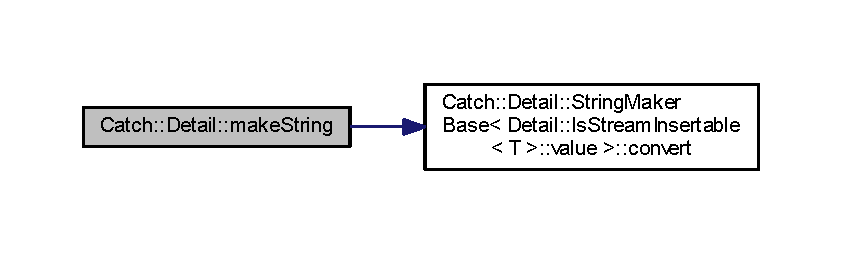
\includegraphics[width=350pt]{namespace_catch_1_1_detail_aef46b4178e08758524d25d1d969a503c_cgraph}
\end{center}
\end{figure}
Here is the caller graph for this function\+:\nopagebreak
\begin{figure}[H]
\begin{center}
\leavevmode
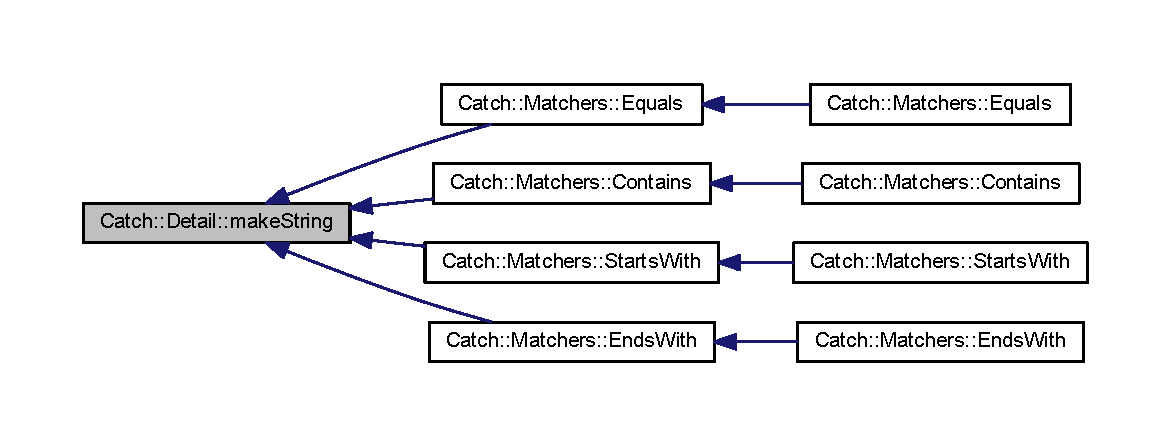
\includegraphics[width=350pt]{namespace_catch_1_1_detail_aef46b4178e08758524d25d1d969a503c_icgraph}
\end{center}
\end{figure}
\hypertarget{namespace_catch_1_1_detail_ae9a44d574c4fbd18fabaaee05a433d88}{}\label{namespace_catch_1_1_detail_ae9a44d574c4fbd18fabaaee05a433d88} 
\index{Catch\+::\+Detail@{Catch\+::\+Detail}!operator$<$$<$@{operator$<$$<$}}
\index{operator$<$$<$@{operator$<$$<$}!Catch\+::\+Detail@{Catch\+::\+Detail}}
\subsubsection{\texorpdfstring{operator$<$$<$()}{operator<<()}}
{\footnotesize\ttfamily \hyperlink{struct_catch_1_1_detail_1_1_false_type}{False\+Type} Catch\+::\+Detail\+::operator$<$$<$ (\begin{DoxyParamCaption}\item[{std\+::ostream const \&}]{,  }\item[{\hyperlink{struct_catch_1_1_detail_1_1_borg_type}{Borg\+Type} const \&}]{ }\end{DoxyParamCaption})}

\hypertarget{namespace_catch_1_1_detail_a6650a1dff325bf29962ff15ae73fd972}{}\label{namespace_catch_1_1_detail_a6650a1dff325bf29962ff15ae73fd972} 
\index{Catch\+::\+Detail@{Catch\+::\+Detail}!range\+To\+String@{range\+To\+String}}
\index{range\+To\+String@{range\+To\+String}!Catch\+::\+Detail@{Catch\+::\+Detail}}
\subsubsection{\texorpdfstring{range\+To\+String()}{rangeToString()}}
{\footnotesize\ttfamily template$<$typename Input\+Iterator $>$ \\
std\+::string Catch\+::\+Detail\+::range\+To\+String (\begin{DoxyParamCaption}\item[{Input\+Iterator}]{first,  }\item[{Input\+Iterator}]{last }\end{DoxyParamCaption})}

Here is the call graph for this function\+:\nopagebreak
\begin{figure}[H]
\begin{center}
\leavevmode
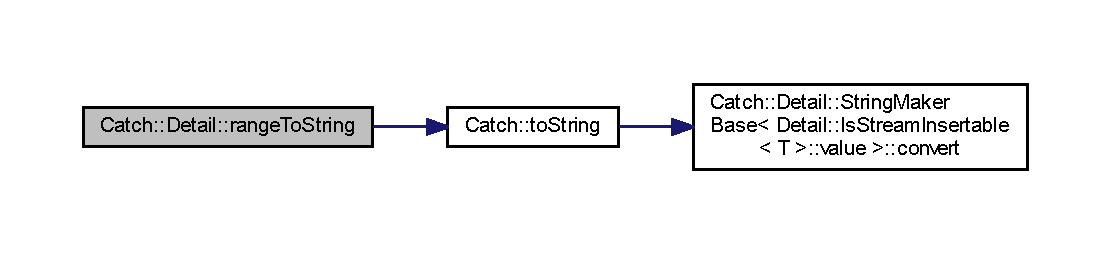
\includegraphics[width=350pt]{namespace_catch_1_1_detail_a6650a1dff325bf29962ff15ae73fd972_cgraph}
\end{center}
\end{figure}
Here is the caller graph for this function\+:\nopagebreak
\begin{figure}[H]
\begin{center}
\leavevmode
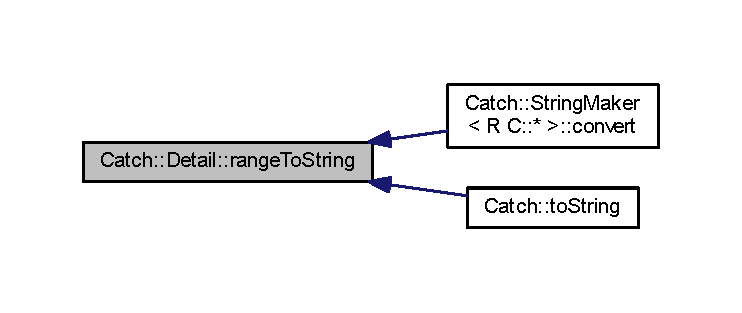
\includegraphics[width=350pt]{namespace_catch_1_1_detail_a6650a1dff325bf29962ff15ae73fd972_icgraph}
\end{center}
\end{figure}
\hypertarget{namespace_catch_1_1_detail_ac5d6c510e565ee5bddcc2236194ce29e}{}\label{namespace_catch_1_1_detail_ac5d6c510e565ee5bddcc2236194ce29e} 
\index{Catch\+::\+Detail@{Catch\+::\+Detail}!raw\+Memory\+To\+String@{raw\+Memory\+To\+String}}
\index{raw\+Memory\+To\+String@{raw\+Memory\+To\+String}!Catch\+::\+Detail@{Catch\+::\+Detail}}
\subsubsection{\texorpdfstring{raw\+Memory\+To\+String()}{rawMemoryToString()}\hspace{0.1cm}{\footnotesize\ttfamily [1/2]}}
{\footnotesize\ttfamily std\+::string Catch\+::\+Detail\+::raw\+Memory\+To\+String (\begin{DoxyParamCaption}\item[{const void $\ast$}]{object,  }\item[{std\+::size\+\_\+t}]{size }\end{DoxyParamCaption})}

Here is the caller graph for this function\+:\nopagebreak
\begin{figure}[H]
\begin{center}
\leavevmode
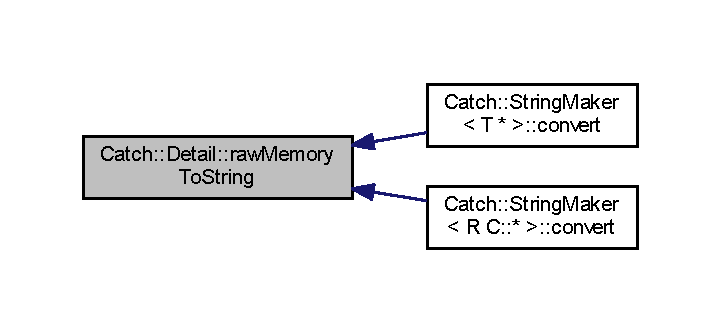
\includegraphics[width=346pt]{namespace_catch_1_1_detail_ac5d6c510e565ee5bddcc2236194ce29e_icgraph}
\end{center}
\end{figure}
\hypertarget{namespace_catch_1_1_detail_a371620ed524abfcae5c3772bf49b563a}{}\label{namespace_catch_1_1_detail_a371620ed524abfcae5c3772bf49b563a} 
\index{Catch\+::\+Detail@{Catch\+::\+Detail}!raw\+Memory\+To\+String@{raw\+Memory\+To\+String}}
\index{raw\+Memory\+To\+String@{raw\+Memory\+To\+String}!Catch\+::\+Detail@{Catch\+::\+Detail}}
\subsubsection{\texorpdfstring{raw\+Memory\+To\+String()}{rawMemoryToString()}\hspace{0.1cm}{\footnotesize\ttfamily [2/2]}}
{\footnotesize\ttfamily template$<$typename T $>$ \\
std\+::string Catch\+::\+Detail\+::raw\+Memory\+To\+String (\begin{DoxyParamCaption}\item[{const T \&}]{object }\end{DoxyParamCaption})\hspace{0.3cm}{\ttfamily [inline]}}

Here is the caller graph for this function\+:\nopagebreak
\begin{figure}[H]
\begin{center}
\leavevmode
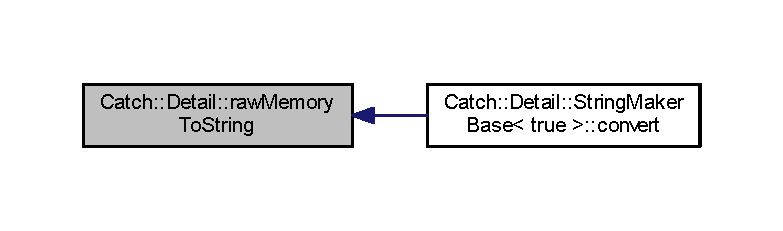
\includegraphics[width=350pt]{namespace_catch_1_1_detail_a371620ed524abfcae5c3772bf49b563a_icgraph}
\end{center}
\end{figure}
\hypertarget{namespace_catch_1_1_detail_aff0ca0f561ad8053654ab27d54486197}{}\label{namespace_catch_1_1_detail_aff0ca0f561ad8053654ab27d54486197} 
\index{Catch\+::\+Detail@{Catch\+::\+Detail}!test\+Streamable@{test\+Streamable}}
\index{test\+Streamable@{test\+Streamable}!Catch\+::\+Detail@{Catch\+::\+Detail}}
\subsubsection{\texorpdfstring{test\+Streamable()}{testStreamable()}\hspace{0.1cm}{\footnotesize\ttfamily [1/2]}}
{\footnotesize\ttfamily \hyperlink{struct_catch_1_1_detail_1_1_true_type}{True\+Type}\& Catch\+::\+Detail\+::test\+Streamable (\begin{DoxyParamCaption}\item[{std\+::ostream \&}]{ }\end{DoxyParamCaption})}

\hypertarget{namespace_catch_1_1_detail_aac81f01b0d687f75b8f24a925591b7ac}{}\label{namespace_catch_1_1_detail_aac81f01b0d687f75b8f24a925591b7ac} 
\index{Catch\+::\+Detail@{Catch\+::\+Detail}!test\+Streamable@{test\+Streamable}}
\index{test\+Streamable@{test\+Streamable}!Catch\+::\+Detail@{Catch\+::\+Detail}}
\subsubsection{\texorpdfstring{test\+Streamable()}{testStreamable()}\hspace{0.1cm}{\footnotesize\ttfamily [2/2]}}
{\footnotesize\ttfamily \hyperlink{struct_catch_1_1_detail_1_1_false_type}{False\+Type} Catch\+::\+Detail\+::test\+Streamable (\begin{DoxyParamCaption}\item[{\hyperlink{struct_catch_1_1_detail_1_1_false_type}{False\+Type}}]{ }\end{DoxyParamCaption})}



\subsection{Variable Documentation}
\hypertarget{namespace_catch_1_1_detail_a466775f4eec29ffef29ab334cd885136}{}\label{namespace_catch_1_1_detail_a466775f4eec29ffef29ab334cd885136} 
\index{Catch\+::\+Detail@{Catch\+::\+Detail}!unprintable\+String@{unprintable\+String}}
\index{unprintable\+String@{unprintable\+String}!Catch\+::\+Detail@{Catch\+::\+Detail}}
\subsubsection{\texorpdfstring{unprintable\+String}{unprintableString}}
{\footnotesize\ttfamily const std\+::string Catch\+::\+Detail\+::unprintable\+String}


\hypertarget{namespace_catch_1_1_generators}{}\section{Catch\+:\+:Generators Namespace Reference}
\label{namespace_catch_1_1_generators}\index{Catch\+::\+Generators@{Catch\+::\+Generators}}
\subsection*{Functions}
\begin{DoxyCompactItemize}
\item 
{\footnotesize template$<$typename T $>$ }\\\hyperlink{class_catch_1_1_composite_generator}{Composite\+Generator}$<$ T $>$ \hyperlink{namespace_catch_1_1_generators_a030abfa7ee3c58d909cf6a6aa0405265}{between} (T from, T to)
\item 
{\footnotesize template$<$typename T $>$ }\\\hyperlink{class_catch_1_1_composite_generator}{Composite\+Generator}$<$ T $>$ \hyperlink{namespace_catch_1_1_generators_a7a2c5bebb3c06c5b0ca05a80289b9eb1}{values} (T val1, T val2)
\item 
{\footnotesize template$<$typename T $>$ }\\\hyperlink{class_catch_1_1_composite_generator}{Composite\+Generator}$<$ T $>$ \hyperlink{namespace_catch_1_1_generators_a496c4a826107e47203b6c609cfd8c2c5}{values} (T val1, T val2, T val3)
\item 
{\footnotesize template$<$typename T $>$ }\\\hyperlink{class_catch_1_1_composite_generator}{Composite\+Generator}$<$ T $>$ \hyperlink{namespace_catch_1_1_generators_afb1dcf02bfc8cdf990f27fdc7d7e4a4e}{values} (T val1, T val2, T val3, T val4)
\end{DoxyCompactItemize}


\subsection{Function Documentation}
\hypertarget{namespace_catch_1_1_generators_a030abfa7ee3c58d909cf6a6aa0405265}{}\label{namespace_catch_1_1_generators_a030abfa7ee3c58d909cf6a6aa0405265} 
\index{Catch\+::\+Generators@{Catch\+::\+Generators}!between@{between}}
\index{between@{between}!Catch\+::\+Generators@{Catch\+::\+Generators}}
\subsubsection{\texorpdfstring{between()}{between()}}
{\footnotesize\ttfamily template$<$typename T $>$ \\
\hyperlink{class_catch_1_1_composite_generator}{Composite\+Generator}$<$T$>$ Catch\+::\+Generators\+::between (\begin{DoxyParamCaption}\item[{T}]{from,  }\item[{T}]{to }\end{DoxyParamCaption})}

Here is the call graph for this function\+:\nopagebreak
\begin{figure}[H]
\begin{center}
\leavevmode
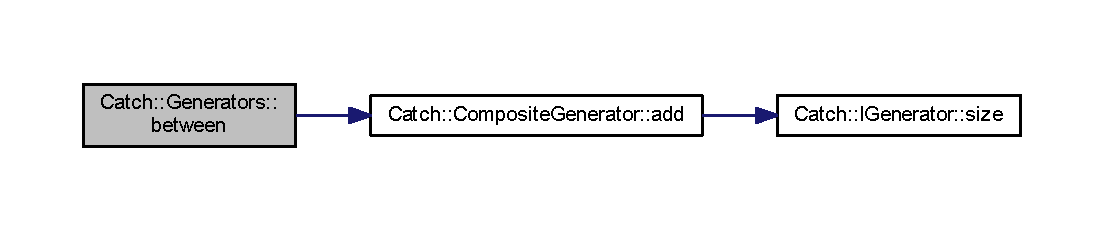
\includegraphics[width=350pt]{namespace_catch_1_1_generators_a030abfa7ee3c58d909cf6a6aa0405265_cgraph}
\end{center}
\end{figure}
\hypertarget{namespace_catch_1_1_generators_a7a2c5bebb3c06c5b0ca05a80289b9eb1}{}\label{namespace_catch_1_1_generators_a7a2c5bebb3c06c5b0ca05a80289b9eb1} 
\index{Catch\+::\+Generators@{Catch\+::\+Generators}!values@{values}}
\index{values@{values}!Catch\+::\+Generators@{Catch\+::\+Generators}}
\subsubsection{\texorpdfstring{values()}{values()}\hspace{0.1cm}{\footnotesize\ttfamily [1/3]}}
{\footnotesize\ttfamily template$<$typename T $>$ \\
\hyperlink{class_catch_1_1_composite_generator}{Composite\+Generator}$<$T$>$ Catch\+::\+Generators\+::values (\begin{DoxyParamCaption}\item[{T}]{val1,  }\item[{T}]{val2 }\end{DoxyParamCaption})}

Here is the call graph for this function\+:\nopagebreak
\begin{figure}[H]
\begin{center}
\leavevmode
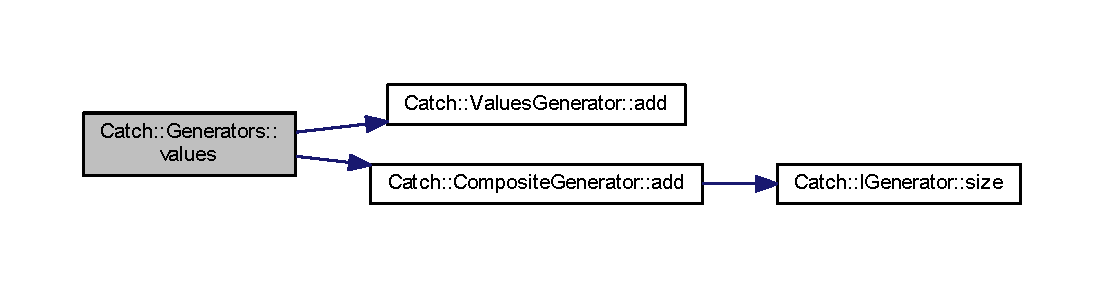
\includegraphics[width=350pt]{namespace_catch_1_1_generators_a7a2c5bebb3c06c5b0ca05a80289b9eb1_cgraph}
\end{center}
\end{figure}
\hypertarget{namespace_catch_1_1_generators_a496c4a826107e47203b6c609cfd8c2c5}{}\label{namespace_catch_1_1_generators_a496c4a826107e47203b6c609cfd8c2c5} 
\index{Catch\+::\+Generators@{Catch\+::\+Generators}!values@{values}}
\index{values@{values}!Catch\+::\+Generators@{Catch\+::\+Generators}}
\subsubsection{\texorpdfstring{values()}{values()}\hspace{0.1cm}{\footnotesize\ttfamily [2/3]}}
{\footnotesize\ttfamily template$<$typename T $>$ \\
\hyperlink{class_catch_1_1_composite_generator}{Composite\+Generator}$<$T$>$ Catch\+::\+Generators\+::values (\begin{DoxyParamCaption}\item[{T}]{val1,  }\item[{T}]{val2,  }\item[{T}]{val3 }\end{DoxyParamCaption})}

Here is the call graph for this function\+:\nopagebreak
\begin{figure}[H]
\begin{center}
\leavevmode
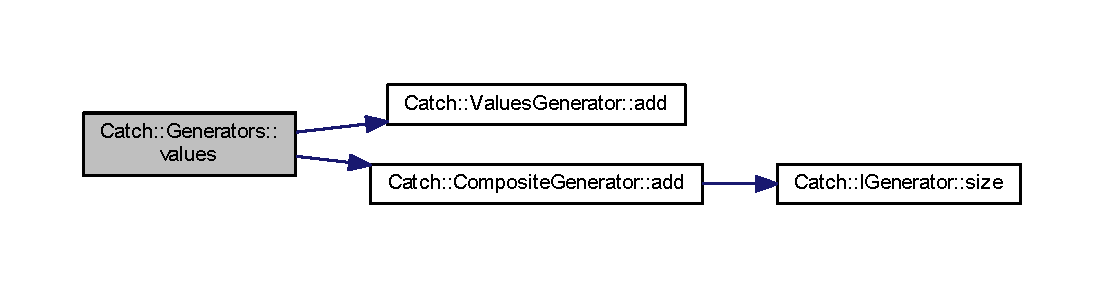
\includegraphics[width=350pt]{namespace_catch_1_1_generators_a496c4a826107e47203b6c609cfd8c2c5_cgraph}
\end{center}
\end{figure}
\hypertarget{namespace_catch_1_1_generators_afb1dcf02bfc8cdf990f27fdc7d7e4a4e}{}\label{namespace_catch_1_1_generators_afb1dcf02bfc8cdf990f27fdc7d7e4a4e} 
\index{Catch\+::\+Generators@{Catch\+::\+Generators}!values@{values}}
\index{values@{values}!Catch\+::\+Generators@{Catch\+::\+Generators}}
\subsubsection{\texorpdfstring{values()}{values()}\hspace{0.1cm}{\footnotesize\ttfamily [3/3]}}
{\footnotesize\ttfamily template$<$typename T $>$ \\
\hyperlink{class_catch_1_1_composite_generator}{Composite\+Generator}$<$T$>$ Catch\+::\+Generators\+::values (\begin{DoxyParamCaption}\item[{T}]{val1,  }\item[{T}]{val2,  }\item[{T}]{val3,  }\item[{T}]{val4 }\end{DoxyParamCaption})}

Here is the call graph for this function\+:\nopagebreak
\begin{figure}[H]
\begin{center}
\leavevmode
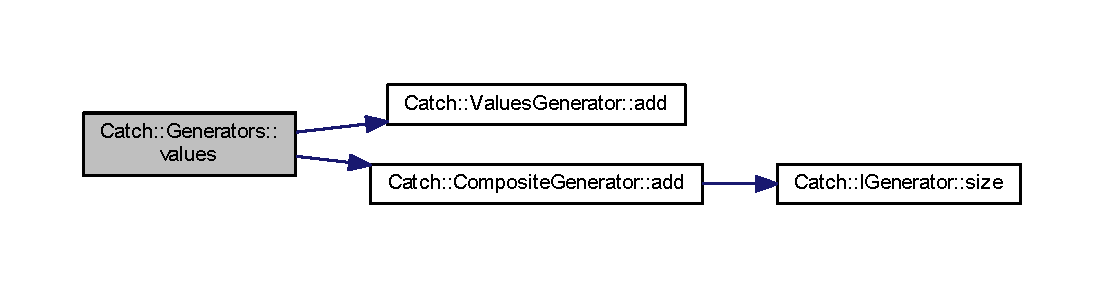
\includegraphics[width=350pt]{namespace_catch_1_1_generators_afb1dcf02bfc8cdf990f27fdc7d7e4a4e_cgraph}
\end{center}
\end{figure}

\hypertarget{namespace_catch_1_1_internal}{}\section{Catch\+:\+:Internal Namespace Reference}
\label{namespace_catch_1_1_internal}\index{Catch\+::\+Internal@{Catch\+::\+Internal}}
\subsection*{Classes}
\begin{DoxyCompactItemize}
\item 
class \hyperlink{class_catch_1_1_internal_1_1_evaluator}{Evaluator}
\item 
struct \hyperlink{struct_catch_1_1_internal_1_1_evaluator_3_01_t1_00_01_t2_00_01_is_equal_to_01_4}{Evaluator$<$ T1, T2, Is\+Equal\+To $>$}
\item 
struct \hyperlink{struct_catch_1_1_internal_1_1_evaluator_3_01_t1_00_01_t2_00_01_is_greater_than_01_4}{Evaluator$<$ T1, T2, Is\+Greater\+Than $>$}
\item 
struct \hyperlink{struct_catch_1_1_internal_1_1_evaluator_3_01_t1_00_01_t2_00_01_is_greater_than_or_equal_to_01_4}{Evaluator$<$ T1, T2, Is\+Greater\+Than\+Or\+Equal\+To $>$}
\item 
struct \hyperlink{struct_catch_1_1_internal_1_1_evaluator_3_01_t1_00_01_t2_00_01_is_less_than_01_4}{Evaluator$<$ T1, T2, Is\+Less\+Than $>$}
\item 
struct \hyperlink{struct_catch_1_1_internal_1_1_evaluator_3_01_t1_00_01_t2_00_01_is_less_than_or_equal_to_01_4}{Evaluator$<$ T1, T2, Is\+Less\+Than\+Or\+Equal\+To $>$}
\item 
struct \hyperlink{struct_catch_1_1_internal_1_1_evaluator_3_01_t1_00_01_t2_00_01_is_not_equal_to_01_4}{Evaluator$<$ T1, T2, Is\+Not\+Equal\+To $>$}
\item 
struct \hyperlink{struct_catch_1_1_internal_1_1_operator_traits}{Operator\+Traits}
\item 
struct \hyperlink{struct_catch_1_1_internal_1_1_operator_traits_3_01_is_equal_to_01_4}{Operator\+Traits$<$ Is\+Equal\+To $>$}
\item 
struct \hyperlink{struct_catch_1_1_internal_1_1_operator_traits_3_01_is_greater_than_01_4}{Operator\+Traits$<$ Is\+Greater\+Than $>$}
\item 
struct \hyperlink{struct_catch_1_1_internal_1_1_operator_traits_3_01_is_greater_than_or_equal_to_01_4}{Operator\+Traits$<$ Is\+Greater\+Than\+Or\+Equal\+To $>$}
\item 
struct \hyperlink{struct_catch_1_1_internal_1_1_operator_traits_3_01_is_less_than_01_4}{Operator\+Traits$<$ Is\+Less\+Than $>$}
\item 
struct \hyperlink{struct_catch_1_1_internal_1_1_operator_traits_3_01_is_less_than_or_equal_to_01_4}{Operator\+Traits$<$ Is\+Less\+Than\+Or\+Equal\+To $>$}
\item 
struct \hyperlink{struct_catch_1_1_internal_1_1_operator_traits_3_01_is_not_equal_to_01_4}{Operator\+Traits$<$ Is\+Not\+Equal\+To $>$}
\end{DoxyCompactItemize}
\subsection*{Enumerations}
\begin{DoxyCompactItemize}
\item 
enum \hyperlink{namespace_catch_1_1_internal_ae3f96598a7858155750bf38e7295d83e}{Operator} \{ \newline
\hyperlink{namespace_catch_1_1_internal_ae3f96598a7858155750bf38e7295d83ea30e0accba6ec8384f4383b04dd2a6a9e}{Is\+Equal\+To}, 
\hyperlink{namespace_catch_1_1_internal_ae3f96598a7858155750bf38e7295d83ea1e1699cf7d3dbee0908f1a123da2456d}{Is\+Not\+Equal\+To}, 
\hyperlink{namespace_catch_1_1_internal_ae3f96598a7858155750bf38e7295d83eabbbfc41706595e50acbefa8408004b93}{Is\+Less\+Than}, 
\hyperlink{namespace_catch_1_1_internal_ae3f96598a7858155750bf38e7295d83eac0e8866139e99803d169595af70f6c22}{Is\+Greater\+Than}, 
\newline
\hyperlink{namespace_catch_1_1_internal_ae3f96598a7858155750bf38e7295d83ea0db29a4c3f1e81260036c5e27a8407fd}{Is\+Less\+Than\+Or\+Equal\+To}, 
\hyperlink{namespace_catch_1_1_internal_ae3f96598a7858155750bf38e7295d83ead2de7e9565e59e36c0987e402203ce1c}{Is\+Greater\+Than\+Or\+Equal\+To}
 \}
\end{DoxyCompactItemize}
\subsection*{Functions}
\begin{DoxyCompactItemize}
\item 
{\footnotesize template$<$typename T $>$ }\\T \& \hyperlink{namespace_catch_1_1_internal_adde98c1a650e94615e2b37ab0b3734e2}{op\+Cast} (T const \&t)
\item 
{\footnotesize template$<$Operator Op, typename T1 , typename T2 $>$ }\\bool \hyperlink{namespace_catch_1_1_internal_a3849d993997f2b708281ff02e77dfecf}{apply\+Evaluator} (T1 const \&lhs, T2 const \&rhs)
\item 
{\footnotesize template$<$Operator Op, typename T1 , typename T2 $>$ }\\bool \hyperlink{namespace_catch_1_1_internal_a64ae04769c4583b9d4027c792b496c7d}{compare} (T1 const \&lhs, T2 const \&rhs)
\item 
{\footnotesize template$<$Operator Op$>$ }\\bool \hyperlink{namespace_catch_1_1_internal_a171aec1826898b877980a2b15fe5f735}{compare} (unsigned int lhs, int rhs)
\item 
{\footnotesize template$<$Operator Op$>$ }\\bool \hyperlink{namespace_catch_1_1_internal_aa2698c33ec87b16aff5c844165483a7a}{compare} (unsigned long lhs, int rhs)
\item 
{\footnotesize template$<$Operator Op$>$ }\\bool \hyperlink{namespace_catch_1_1_internal_ad68724393ee3d7629001a2997f6134cc}{compare} (unsigned char lhs, int rhs)
\item 
{\footnotesize template$<$Operator Op$>$ }\\bool \hyperlink{namespace_catch_1_1_internal_ac2af7b6757f9bb3539bb78acff5c4649}{compare} (unsigned int lhs, long rhs)
\item 
{\footnotesize template$<$Operator Op$>$ }\\bool \hyperlink{namespace_catch_1_1_internal_ace20062a489a8a7049fe224d62e644a7}{compare} (unsigned long lhs, long rhs)
\item 
{\footnotesize template$<$Operator Op$>$ }\\bool \hyperlink{namespace_catch_1_1_internal_a640e0cce9260a912842bee58db501dc5}{compare} (unsigned char lhs, long rhs)
\item 
{\footnotesize template$<$Operator Op$>$ }\\bool \hyperlink{namespace_catch_1_1_internal_a17c92ed4b6d88a9f8bbcbc52544fe40f}{compare} (int lhs, unsigned int rhs)
\item 
{\footnotesize template$<$Operator Op$>$ }\\bool \hyperlink{namespace_catch_1_1_internal_aac7a6452ed0d324031ceb7b4f3a3b61c}{compare} (int lhs, unsigned long rhs)
\item 
{\footnotesize template$<$Operator Op$>$ }\\bool \hyperlink{namespace_catch_1_1_internal_a7e82d987f62b9822107027c72a55fa6b}{compare} (int lhs, unsigned char rhs)
\item 
{\footnotesize template$<$Operator Op$>$ }\\bool \hyperlink{namespace_catch_1_1_internal_a0b4783ede1901e5c1baf8ff909bcce8d}{compare} (long lhs, unsigned int rhs)
\item 
{\footnotesize template$<$Operator Op$>$ }\\bool \hyperlink{namespace_catch_1_1_internal_ae9aec44a08d9cbb0d3dd46d438b50d2c}{compare} (long lhs, unsigned long rhs)
\item 
{\footnotesize template$<$Operator Op$>$ }\\bool \hyperlink{namespace_catch_1_1_internal_a79664b5f5f497fba57bd156e098de1f2}{compare} (long lhs, unsigned char rhs)
\item 
{\footnotesize template$<$Operator Op, typename T $>$ }\\bool \hyperlink{namespace_catch_1_1_internal_a829570ad9e724c687aa42190a696032b}{compare} (long lhs, T $\ast$rhs)
\item 
{\footnotesize template$<$Operator Op, typename T $>$ }\\bool \hyperlink{namespace_catch_1_1_internal_a3f89c65fdb06aa7b648c5acf0ca107a9}{compare} (T $\ast$lhs, long rhs)
\item 
{\footnotesize template$<$Operator Op, typename T $>$ }\\bool \hyperlink{namespace_catch_1_1_internal_a4f30c29e4adb62c7e209e5b988e59397}{compare} (int lhs, T $\ast$rhs)
\item 
{\footnotesize template$<$Operator Op, typename T $>$ }\\bool \hyperlink{namespace_catch_1_1_internal_a95361ddae55c9a390e6510bdadccb1fc}{compare} (T $\ast$lhs, int rhs)
\end{DoxyCompactItemize}


\subsection{Enumeration Type Documentation}
\hypertarget{namespace_catch_1_1_internal_ae3f96598a7858155750bf38e7295d83e}{}\label{namespace_catch_1_1_internal_ae3f96598a7858155750bf38e7295d83e} 
\index{Catch\+::\+Internal@{Catch\+::\+Internal}!Operator@{Operator}}
\index{Operator@{Operator}!Catch\+::\+Internal@{Catch\+::\+Internal}}
\subsubsection{\texorpdfstring{Operator}{Operator}}
{\footnotesize\ttfamily enum \hyperlink{namespace_catch_1_1_internal_ae3f96598a7858155750bf38e7295d83e}{Catch\+::\+Internal\+::\+Operator}}

\begin{DoxyEnumFields}{Enumerator}
\raisebox{\heightof{T}}[0pt][0pt]{\index{Is\+Equal\+To@{Is\+Equal\+To}!Catch\+::\+Internal@{Catch\+::\+Internal}}\index{Catch\+::\+Internal@{Catch\+::\+Internal}!Is\+Equal\+To@{Is\+Equal\+To}}}\hypertarget{namespace_catch_1_1_internal_ae3f96598a7858155750bf38e7295d83ea30e0accba6ec8384f4383b04dd2a6a9e}{}\label{namespace_catch_1_1_internal_ae3f96598a7858155750bf38e7295d83ea30e0accba6ec8384f4383b04dd2a6a9e} 
Is\+Equal\+To&\\
\hline

\raisebox{\heightof{T}}[0pt][0pt]{\index{Is\+Not\+Equal\+To@{Is\+Not\+Equal\+To}!Catch\+::\+Internal@{Catch\+::\+Internal}}\index{Catch\+::\+Internal@{Catch\+::\+Internal}!Is\+Not\+Equal\+To@{Is\+Not\+Equal\+To}}}\hypertarget{namespace_catch_1_1_internal_ae3f96598a7858155750bf38e7295d83ea1e1699cf7d3dbee0908f1a123da2456d}{}\label{namespace_catch_1_1_internal_ae3f96598a7858155750bf38e7295d83ea1e1699cf7d3dbee0908f1a123da2456d} 
Is\+Not\+Equal\+To&\\
\hline

\raisebox{\heightof{T}}[0pt][0pt]{\index{Is\+Less\+Than@{Is\+Less\+Than}!Catch\+::\+Internal@{Catch\+::\+Internal}}\index{Catch\+::\+Internal@{Catch\+::\+Internal}!Is\+Less\+Than@{Is\+Less\+Than}}}\hypertarget{namespace_catch_1_1_internal_ae3f96598a7858155750bf38e7295d83eabbbfc41706595e50acbefa8408004b93}{}\label{namespace_catch_1_1_internal_ae3f96598a7858155750bf38e7295d83eabbbfc41706595e50acbefa8408004b93} 
Is\+Less\+Than&\\
\hline

\raisebox{\heightof{T}}[0pt][0pt]{\index{Is\+Greater\+Than@{Is\+Greater\+Than}!Catch\+::\+Internal@{Catch\+::\+Internal}}\index{Catch\+::\+Internal@{Catch\+::\+Internal}!Is\+Greater\+Than@{Is\+Greater\+Than}}}\hypertarget{namespace_catch_1_1_internal_ae3f96598a7858155750bf38e7295d83eac0e8866139e99803d169595af70f6c22}{}\label{namespace_catch_1_1_internal_ae3f96598a7858155750bf38e7295d83eac0e8866139e99803d169595af70f6c22} 
Is\+Greater\+Than&\\
\hline

\raisebox{\heightof{T}}[0pt][0pt]{\index{Is\+Less\+Than\+Or\+Equal\+To@{Is\+Less\+Than\+Or\+Equal\+To}!Catch\+::\+Internal@{Catch\+::\+Internal}}\index{Catch\+::\+Internal@{Catch\+::\+Internal}!Is\+Less\+Than\+Or\+Equal\+To@{Is\+Less\+Than\+Or\+Equal\+To}}}\hypertarget{namespace_catch_1_1_internal_ae3f96598a7858155750bf38e7295d83ea0db29a4c3f1e81260036c5e27a8407fd}{}\label{namespace_catch_1_1_internal_ae3f96598a7858155750bf38e7295d83ea0db29a4c3f1e81260036c5e27a8407fd} 
Is\+Less\+Than\+Or\+Equal\+To&\\
\hline

\raisebox{\heightof{T}}[0pt][0pt]{\index{Is\+Greater\+Than\+Or\+Equal\+To@{Is\+Greater\+Than\+Or\+Equal\+To}!Catch\+::\+Internal@{Catch\+::\+Internal}}\index{Catch\+::\+Internal@{Catch\+::\+Internal}!Is\+Greater\+Than\+Or\+Equal\+To@{Is\+Greater\+Than\+Or\+Equal\+To}}}\hypertarget{namespace_catch_1_1_internal_ae3f96598a7858155750bf38e7295d83ead2de7e9565e59e36c0987e402203ce1c}{}\label{namespace_catch_1_1_internal_ae3f96598a7858155750bf38e7295d83ead2de7e9565e59e36c0987e402203ce1c} 
Is\+Greater\+Than\+Or\+Equal\+To&\\
\hline

\end{DoxyEnumFields}


Definition at line 1303 of file catch.\+hpp.



\subsection{Function Documentation}
\hypertarget{namespace_catch_1_1_internal_a3849d993997f2b708281ff02e77dfecf}{}\label{namespace_catch_1_1_internal_a3849d993997f2b708281ff02e77dfecf} 
\index{Catch\+::\+Internal@{Catch\+::\+Internal}!apply\+Evaluator@{apply\+Evaluator}}
\index{apply\+Evaluator@{apply\+Evaluator}!Catch\+::\+Internal@{Catch\+::\+Internal}}
\subsubsection{\texorpdfstring{apply\+Evaluator()}{applyEvaluator()}}
{\footnotesize\ttfamily template$<$Operator Op, typename T1 , typename T2 $>$ \\
bool Catch\+::\+Internal\+::apply\+Evaluator (\begin{DoxyParamCaption}\item[{T1 const \&}]{lhs,  }\item[{T2 const \&}]{rhs }\end{DoxyParamCaption})}



Definition at line 1371 of file catch.\+hpp.

\hypertarget{namespace_catch_1_1_internal_a64ae04769c4583b9d4027c792b496c7d}{}\label{namespace_catch_1_1_internal_a64ae04769c4583b9d4027c792b496c7d} 
\index{Catch\+::\+Internal@{Catch\+::\+Internal}!compare@{compare}}
\index{compare@{compare}!Catch\+::\+Internal@{Catch\+::\+Internal}}
\subsubsection{\texorpdfstring{compare()}{compare()}\hspace{0.1cm}{\footnotesize\ttfamily [1/17]}}
{\footnotesize\ttfamily template$<$Operator Op, typename T1 , typename T2 $>$ \\
bool Catch\+::\+Internal\+::compare (\begin{DoxyParamCaption}\item[{T1 const \&}]{lhs,  }\item[{T2 const \&}]{rhs }\end{DoxyParamCaption})}



Definition at line 1380 of file catch.\+hpp.

\hypertarget{namespace_catch_1_1_internal_a171aec1826898b877980a2b15fe5f735}{}\label{namespace_catch_1_1_internal_a171aec1826898b877980a2b15fe5f735} 
\index{Catch\+::\+Internal@{Catch\+::\+Internal}!compare@{compare}}
\index{compare@{compare}!Catch\+::\+Internal@{Catch\+::\+Internal}}
\subsubsection{\texorpdfstring{compare()}{compare()}\hspace{0.1cm}{\footnotesize\ttfamily [2/17]}}
{\footnotesize\ttfamily template$<$Operator Op$>$ \\
bool Catch\+::\+Internal\+::compare (\begin{DoxyParamCaption}\item[{unsigned int}]{lhs,  }\item[{int}]{rhs }\end{DoxyParamCaption})}



Definition at line 1385 of file catch.\+hpp.

\hypertarget{namespace_catch_1_1_internal_aa2698c33ec87b16aff5c844165483a7a}{}\label{namespace_catch_1_1_internal_aa2698c33ec87b16aff5c844165483a7a} 
\index{Catch\+::\+Internal@{Catch\+::\+Internal}!compare@{compare}}
\index{compare@{compare}!Catch\+::\+Internal@{Catch\+::\+Internal}}
\subsubsection{\texorpdfstring{compare()}{compare()}\hspace{0.1cm}{\footnotesize\ttfamily [3/17]}}
{\footnotesize\ttfamily template$<$Operator Op$>$ \\
bool Catch\+::\+Internal\+::compare (\begin{DoxyParamCaption}\item[{unsigned long}]{lhs,  }\item[{int}]{rhs }\end{DoxyParamCaption})}



Definition at line 1388 of file catch.\+hpp.

\hypertarget{namespace_catch_1_1_internal_ad68724393ee3d7629001a2997f6134cc}{}\label{namespace_catch_1_1_internal_ad68724393ee3d7629001a2997f6134cc} 
\index{Catch\+::\+Internal@{Catch\+::\+Internal}!compare@{compare}}
\index{compare@{compare}!Catch\+::\+Internal@{Catch\+::\+Internal}}
\subsubsection{\texorpdfstring{compare()}{compare()}\hspace{0.1cm}{\footnotesize\ttfamily [4/17]}}
{\footnotesize\ttfamily template$<$Operator Op$>$ \\
bool Catch\+::\+Internal\+::compare (\begin{DoxyParamCaption}\item[{unsigned char}]{lhs,  }\item[{int}]{rhs }\end{DoxyParamCaption})}



Definition at line 1391 of file catch.\+hpp.

\hypertarget{namespace_catch_1_1_internal_ac2af7b6757f9bb3539bb78acff5c4649}{}\label{namespace_catch_1_1_internal_ac2af7b6757f9bb3539bb78acff5c4649} 
\index{Catch\+::\+Internal@{Catch\+::\+Internal}!compare@{compare}}
\index{compare@{compare}!Catch\+::\+Internal@{Catch\+::\+Internal}}
\subsubsection{\texorpdfstring{compare()}{compare()}\hspace{0.1cm}{\footnotesize\ttfamily [5/17]}}
{\footnotesize\ttfamily template$<$Operator Op$>$ \\
bool Catch\+::\+Internal\+::compare (\begin{DoxyParamCaption}\item[{unsigned int}]{lhs,  }\item[{long}]{rhs }\end{DoxyParamCaption})}



Definition at line 1396 of file catch.\+hpp.

\hypertarget{namespace_catch_1_1_internal_ace20062a489a8a7049fe224d62e644a7}{}\label{namespace_catch_1_1_internal_ace20062a489a8a7049fe224d62e644a7} 
\index{Catch\+::\+Internal@{Catch\+::\+Internal}!compare@{compare}}
\index{compare@{compare}!Catch\+::\+Internal@{Catch\+::\+Internal}}
\subsubsection{\texorpdfstring{compare()}{compare()}\hspace{0.1cm}{\footnotesize\ttfamily [6/17]}}
{\footnotesize\ttfamily template$<$Operator Op$>$ \\
bool Catch\+::\+Internal\+::compare (\begin{DoxyParamCaption}\item[{unsigned long}]{lhs,  }\item[{long}]{rhs }\end{DoxyParamCaption})}



Definition at line 1399 of file catch.\+hpp.

\hypertarget{namespace_catch_1_1_internal_a640e0cce9260a912842bee58db501dc5}{}\label{namespace_catch_1_1_internal_a640e0cce9260a912842bee58db501dc5} 
\index{Catch\+::\+Internal@{Catch\+::\+Internal}!compare@{compare}}
\index{compare@{compare}!Catch\+::\+Internal@{Catch\+::\+Internal}}
\subsubsection{\texorpdfstring{compare()}{compare()}\hspace{0.1cm}{\footnotesize\ttfamily [7/17]}}
{\footnotesize\ttfamily template$<$Operator Op$>$ \\
bool Catch\+::\+Internal\+::compare (\begin{DoxyParamCaption}\item[{unsigned char}]{lhs,  }\item[{long}]{rhs }\end{DoxyParamCaption})}



Definition at line 1402 of file catch.\+hpp.

\hypertarget{namespace_catch_1_1_internal_a17c92ed4b6d88a9f8bbcbc52544fe40f}{}\label{namespace_catch_1_1_internal_a17c92ed4b6d88a9f8bbcbc52544fe40f} 
\index{Catch\+::\+Internal@{Catch\+::\+Internal}!compare@{compare}}
\index{compare@{compare}!Catch\+::\+Internal@{Catch\+::\+Internal}}
\subsubsection{\texorpdfstring{compare()}{compare()}\hspace{0.1cm}{\footnotesize\ttfamily [8/17]}}
{\footnotesize\ttfamily template$<$Operator Op$>$ \\
bool Catch\+::\+Internal\+::compare (\begin{DoxyParamCaption}\item[{int}]{lhs,  }\item[{unsigned int}]{rhs }\end{DoxyParamCaption})}



Definition at line 1407 of file catch.\+hpp.

\hypertarget{namespace_catch_1_1_internal_aac7a6452ed0d324031ceb7b4f3a3b61c}{}\label{namespace_catch_1_1_internal_aac7a6452ed0d324031ceb7b4f3a3b61c} 
\index{Catch\+::\+Internal@{Catch\+::\+Internal}!compare@{compare}}
\index{compare@{compare}!Catch\+::\+Internal@{Catch\+::\+Internal}}
\subsubsection{\texorpdfstring{compare()}{compare()}\hspace{0.1cm}{\footnotesize\ttfamily [9/17]}}
{\footnotesize\ttfamily template$<$Operator Op$>$ \\
bool Catch\+::\+Internal\+::compare (\begin{DoxyParamCaption}\item[{int}]{lhs,  }\item[{unsigned long}]{rhs }\end{DoxyParamCaption})}



Definition at line 1410 of file catch.\+hpp.

\hypertarget{namespace_catch_1_1_internal_a7e82d987f62b9822107027c72a55fa6b}{}\label{namespace_catch_1_1_internal_a7e82d987f62b9822107027c72a55fa6b} 
\index{Catch\+::\+Internal@{Catch\+::\+Internal}!compare@{compare}}
\index{compare@{compare}!Catch\+::\+Internal@{Catch\+::\+Internal}}
\subsubsection{\texorpdfstring{compare()}{compare()}\hspace{0.1cm}{\footnotesize\ttfamily [10/17]}}
{\footnotesize\ttfamily template$<$Operator Op$>$ \\
bool Catch\+::\+Internal\+::compare (\begin{DoxyParamCaption}\item[{int}]{lhs,  }\item[{unsigned char}]{rhs }\end{DoxyParamCaption})}



Definition at line 1413 of file catch.\+hpp.

\hypertarget{namespace_catch_1_1_internal_a0b4783ede1901e5c1baf8ff909bcce8d}{}\label{namespace_catch_1_1_internal_a0b4783ede1901e5c1baf8ff909bcce8d} 
\index{Catch\+::\+Internal@{Catch\+::\+Internal}!compare@{compare}}
\index{compare@{compare}!Catch\+::\+Internal@{Catch\+::\+Internal}}
\subsubsection{\texorpdfstring{compare()}{compare()}\hspace{0.1cm}{\footnotesize\ttfamily [11/17]}}
{\footnotesize\ttfamily template$<$Operator Op$>$ \\
bool Catch\+::\+Internal\+::compare (\begin{DoxyParamCaption}\item[{long}]{lhs,  }\item[{unsigned int}]{rhs }\end{DoxyParamCaption})}



Definition at line 1418 of file catch.\+hpp.

\hypertarget{namespace_catch_1_1_internal_ae9aec44a08d9cbb0d3dd46d438b50d2c}{}\label{namespace_catch_1_1_internal_ae9aec44a08d9cbb0d3dd46d438b50d2c} 
\index{Catch\+::\+Internal@{Catch\+::\+Internal}!compare@{compare}}
\index{compare@{compare}!Catch\+::\+Internal@{Catch\+::\+Internal}}
\subsubsection{\texorpdfstring{compare()}{compare()}\hspace{0.1cm}{\footnotesize\ttfamily [12/17]}}
{\footnotesize\ttfamily template$<$Operator Op$>$ \\
bool Catch\+::\+Internal\+::compare (\begin{DoxyParamCaption}\item[{long}]{lhs,  }\item[{unsigned long}]{rhs }\end{DoxyParamCaption})}



Definition at line 1421 of file catch.\+hpp.

\hypertarget{namespace_catch_1_1_internal_a79664b5f5f497fba57bd156e098de1f2}{}\label{namespace_catch_1_1_internal_a79664b5f5f497fba57bd156e098de1f2} 
\index{Catch\+::\+Internal@{Catch\+::\+Internal}!compare@{compare}}
\index{compare@{compare}!Catch\+::\+Internal@{Catch\+::\+Internal}}
\subsubsection{\texorpdfstring{compare()}{compare()}\hspace{0.1cm}{\footnotesize\ttfamily [13/17]}}
{\footnotesize\ttfamily template$<$Operator Op$>$ \\
bool Catch\+::\+Internal\+::compare (\begin{DoxyParamCaption}\item[{long}]{lhs,  }\item[{unsigned char}]{rhs }\end{DoxyParamCaption})}



Definition at line 1424 of file catch.\+hpp.

\hypertarget{namespace_catch_1_1_internal_a829570ad9e724c687aa42190a696032b}{}\label{namespace_catch_1_1_internal_a829570ad9e724c687aa42190a696032b} 
\index{Catch\+::\+Internal@{Catch\+::\+Internal}!compare@{compare}}
\index{compare@{compare}!Catch\+::\+Internal@{Catch\+::\+Internal}}
\subsubsection{\texorpdfstring{compare()}{compare()}\hspace{0.1cm}{\footnotesize\ttfamily [14/17]}}
{\footnotesize\ttfamily template$<$Operator Op, typename T $>$ \\
bool Catch\+::\+Internal\+::compare (\begin{DoxyParamCaption}\item[{long}]{lhs,  }\item[{T $\ast$}]{rhs }\end{DoxyParamCaption})}



Definition at line 1429 of file catch.\+hpp.

\hypertarget{namespace_catch_1_1_internal_a3f89c65fdb06aa7b648c5acf0ca107a9}{}\label{namespace_catch_1_1_internal_a3f89c65fdb06aa7b648c5acf0ca107a9} 
\index{Catch\+::\+Internal@{Catch\+::\+Internal}!compare@{compare}}
\index{compare@{compare}!Catch\+::\+Internal@{Catch\+::\+Internal}}
\subsubsection{\texorpdfstring{compare()}{compare()}\hspace{0.1cm}{\footnotesize\ttfamily [15/17]}}
{\footnotesize\ttfamily template$<$Operator Op, typename T $>$ \\
bool Catch\+::\+Internal\+::compare (\begin{DoxyParamCaption}\item[{T $\ast$}]{lhs,  }\item[{long}]{rhs }\end{DoxyParamCaption})}



Definition at line 1432 of file catch.\+hpp.

\hypertarget{namespace_catch_1_1_internal_a4f30c29e4adb62c7e209e5b988e59397}{}\label{namespace_catch_1_1_internal_a4f30c29e4adb62c7e209e5b988e59397} 
\index{Catch\+::\+Internal@{Catch\+::\+Internal}!compare@{compare}}
\index{compare@{compare}!Catch\+::\+Internal@{Catch\+::\+Internal}}
\subsubsection{\texorpdfstring{compare()}{compare()}\hspace{0.1cm}{\footnotesize\ttfamily [16/17]}}
{\footnotesize\ttfamily template$<$Operator Op, typename T $>$ \\
bool Catch\+::\+Internal\+::compare (\begin{DoxyParamCaption}\item[{int}]{lhs,  }\item[{T $\ast$}]{rhs }\end{DoxyParamCaption})}



Definition at line 1437 of file catch.\+hpp.

\hypertarget{namespace_catch_1_1_internal_a95361ddae55c9a390e6510bdadccb1fc}{}\label{namespace_catch_1_1_internal_a95361ddae55c9a390e6510bdadccb1fc} 
\index{Catch\+::\+Internal@{Catch\+::\+Internal}!compare@{compare}}
\index{compare@{compare}!Catch\+::\+Internal@{Catch\+::\+Internal}}
\subsubsection{\texorpdfstring{compare()}{compare()}\hspace{0.1cm}{\footnotesize\ttfamily [17/17]}}
{\footnotesize\ttfamily template$<$Operator Op, typename T $>$ \\
bool Catch\+::\+Internal\+::compare (\begin{DoxyParamCaption}\item[{T $\ast$}]{lhs,  }\item[{int}]{rhs }\end{DoxyParamCaption})}



Definition at line 1440 of file catch.\+hpp.

\hypertarget{namespace_catch_1_1_internal_adde98c1a650e94615e2b37ab0b3734e2}{}\label{namespace_catch_1_1_internal_adde98c1a650e94615e2b37ab0b3734e2} 
\index{Catch\+::\+Internal@{Catch\+::\+Internal}!op\+Cast@{op\+Cast}}
\index{op\+Cast@{op\+Cast}!Catch\+::\+Internal@{Catch\+::\+Internal}}
\subsubsection{\texorpdfstring{op\+Cast()}{opCast()}}
{\footnotesize\ttfamily template$<$typename T $>$ \\
T\& Catch\+::\+Internal\+::op\+Cast (\begin{DoxyParamCaption}\item[{T const \&}]{t }\end{DoxyParamCaption})\hspace{0.3cm}{\ttfamily [inline]}}



Definition at line 1321 of file catch.\+hpp.

Here is the caller graph for this function\+:\nopagebreak
\begin{figure}[H]
\begin{center}
\leavevmode
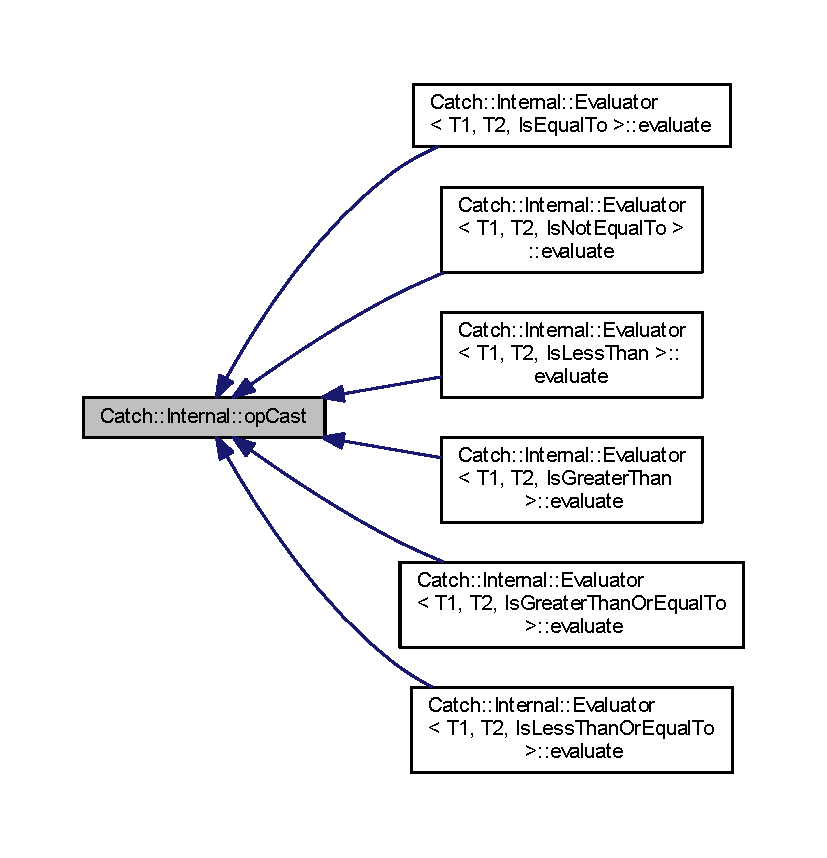
\includegraphics[width=350pt]{namespace_catch_1_1_internal_adde98c1a650e94615e2b37ab0b3734e2_icgraph}
\end{center}
\end{figure}

\hypertarget{namespace_catch_1_1_matchers}{}\section{Catch\+:\+:Matchers Namespace Reference}
\label{namespace_catch_1_1_matchers}\index{Catch\+::\+Matchers@{Catch\+::\+Matchers}}
\subsection*{Namespaces}
\begin{DoxyCompactItemize}
\item 
 \hyperlink{namespace_catch_1_1_matchers_1_1_impl}{Impl}
\end{DoxyCompactItemize}
\subsection*{Functions}
\begin{DoxyCompactItemize}
\item 
{\footnotesize template$<$typename ExpressionT $>$ }\\\hyperlink{class_catch_1_1_matchers_1_1_impl_1_1_generic_1_1_not}{Impl\+::\+Generic\+::\+Not}$<$ ExpressionT $>$ \hyperlink{namespace_catch_1_1_matchers_ae3c192dc15c973c38f07376d4debdc34}{Not} (\hyperlink{struct_catch_1_1_matchers_1_1_impl_1_1_matcher}{Impl\+::\+Matcher}$<$ ExpressionT $>$ const \&m)
\item 
{\footnotesize template$<$typename ExpressionT $>$ }\\\hyperlink{class_catch_1_1_matchers_1_1_impl_1_1_generic_1_1_all_of}{Impl\+::\+Generic\+::\+All\+Of}$<$ ExpressionT $>$ \hyperlink{namespace_catch_1_1_matchers_aca6c1c17e137d989583c97f99705797a}{All\+Of} (\hyperlink{struct_catch_1_1_matchers_1_1_impl_1_1_matcher}{Impl\+::\+Matcher}$<$ ExpressionT $>$ const \&m1, \hyperlink{struct_catch_1_1_matchers_1_1_impl_1_1_matcher}{Impl\+::\+Matcher}$<$ ExpressionT $>$ const \&m2)
\item 
{\footnotesize template$<$typename ExpressionT $>$ }\\\hyperlink{class_catch_1_1_matchers_1_1_impl_1_1_generic_1_1_all_of}{Impl\+::\+Generic\+::\+All\+Of}$<$ ExpressionT $>$ \hyperlink{namespace_catch_1_1_matchers_a990366f7d62d10d9752ad7b24230def0}{All\+Of} (\hyperlink{struct_catch_1_1_matchers_1_1_impl_1_1_matcher}{Impl\+::\+Matcher}$<$ ExpressionT $>$ const \&m1, \hyperlink{struct_catch_1_1_matchers_1_1_impl_1_1_matcher}{Impl\+::\+Matcher}$<$ ExpressionT $>$ const \&m2, \hyperlink{struct_catch_1_1_matchers_1_1_impl_1_1_matcher}{Impl\+::\+Matcher}$<$ ExpressionT $>$ const \&m3)
\item 
{\footnotesize template$<$typename ExpressionT $>$ }\\\hyperlink{class_catch_1_1_matchers_1_1_impl_1_1_generic_1_1_any_of}{Impl\+::\+Generic\+::\+Any\+Of}$<$ ExpressionT $>$ \hyperlink{namespace_catch_1_1_matchers_a9cb139c71b9e391d5fc017764695bf84}{Any\+Of} (\hyperlink{struct_catch_1_1_matchers_1_1_impl_1_1_matcher}{Impl\+::\+Matcher}$<$ ExpressionT $>$ const \&m1, \hyperlink{struct_catch_1_1_matchers_1_1_impl_1_1_matcher}{Impl\+::\+Matcher}$<$ ExpressionT $>$ const \&m2)
\item 
{\footnotesize template$<$typename ExpressionT $>$ }\\\hyperlink{class_catch_1_1_matchers_1_1_impl_1_1_generic_1_1_any_of}{Impl\+::\+Generic\+::\+Any\+Of}$<$ ExpressionT $>$ \hyperlink{namespace_catch_1_1_matchers_a8efb0e533db973b8aff1172fb908db02}{Any\+Of} (\hyperlink{struct_catch_1_1_matchers_1_1_impl_1_1_matcher}{Impl\+::\+Matcher}$<$ ExpressionT $>$ const \&m1, \hyperlink{struct_catch_1_1_matchers_1_1_impl_1_1_matcher}{Impl\+::\+Matcher}$<$ ExpressionT $>$ const \&m2, \hyperlink{struct_catch_1_1_matchers_1_1_impl_1_1_matcher}{Impl\+::\+Matcher}$<$ ExpressionT $>$ const \&m3)
\item 
\hyperlink{struct_catch_1_1_matchers_1_1_impl_1_1_std_string_1_1_equals}{Impl\+::\+Std\+String\+::\+Equals} \hyperlink{namespace_catch_1_1_matchers_a840317a3d0f828642c2f55155068bb97}{Equals} (std\+::string const \&str, \hyperlink{struct_catch_1_1_case_sensitive_aad49d3aee2d97066642fffa919685c6a}{Case\+Sensitive\+::\+Choice} case\+Sensitivity=\hyperlink{struct_catch_1_1_case_sensitive_aad49d3aee2d97066642fffa919685c6aa7c5550b69ec3c502e6f609b67f9613c6}{Case\+Sensitive\+::\+Yes})
\item 
\hyperlink{struct_catch_1_1_matchers_1_1_impl_1_1_std_string_1_1_equals}{Impl\+::\+Std\+String\+::\+Equals} \hyperlink{namespace_catch_1_1_matchers_a7454444261cc4af7ee0b0bc82cf74284}{Equals} (const char $\ast$str, \hyperlink{struct_catch_1_1_case_sensitive_aad49d3aee2d97066642fffa919685c6a}{Case\+Sensitive\+::\+Choice} case\+Sensitivity=\hyperlink{struct_catch_1_1_case_sensitive_aad49d3aee2d97066642fffa919685c6aa7c5550b69ec3c502e6f609b67f9613c6}{Case\+Sensitive\+::\+Yes})
\item 
\hyperlink{struct_catch_1_1_matchers_1_1_impl_1_1_std_string_1_1_contains}{Impl\+::\+Std\+String\+::\+Contains} \hyperlink{namespace_catch_1_1_matchers_a07760045eca8bafb7f6618fae10f1b59}{Contains} (std\+::string const \&substr, \hyperlink{struct_catch_1_1_case_sensitive_aad49d3aee2d97066642fffa919685c6a}{Case\+Sensitive\+::\+Choice} case\+Sensitivity=\hyperlink{struct_catch_1_1_case_sensitive_aad49d3aee2d97066642fffa919685c6aa7c5550b69ec3c502e6f609b67f9613c6}{Case\+Sensitive\+::\+Yes})
\item 
\hyperlink{struct_catch_1_1_matchers_1_1_impl_1_1_std_string_1_1_contains}{Impl\+::\+Std\+String\+::\+Contains} \hyperlink{namespace_catch_1_1_matchers_a7bc27b5c696118cbe54690d6c524b3d9}{Contains} (const char $\ast$substr, \hyperlink{struct_catch_1_1_case_sensitive_aad49d3aee2d97066642fffa919685c6a}{Case\+Sensitive\+::\+Choice} case\+Sensitivity=\hyperlink{struct_catch_1_1_case_sensitive_aad49d3aee2d97066642fffa919685c6aa7c5550b69ec3c502e6f609b67f9613c6}{Case\+Sensitive\+::\+Yes})
\item 
\hyperlink{struct_catch_1_1_matchers_1_1_impl_1_1_std_string_1_1_starts_with}{Impl\+::\+Std\+String\+::\+Starts\+With} \hyperlink{namespace_catch_1_1_matchers_a9b6a7704df7d0717dc6686fd2055ffea}{Starts\+With} (std\+::string const \&substr)
\item 
\hyperlink{struct_catch_1_1_matchers_1_1_impl_1_1_std_string_1_1_starts_with}{Impl\+::\+Std\+String\+::\+Starts\+With} \hyperlink{namespace_catch_1_1_matchers_a031985c11b8c8bb62585b3904f9fd2b0}{Starts\+With} (const char $\ast$substr)
\item 
\hyperlink{struct_catch_1_1_matchers_1_1_impl_1_1_std_string_1_1_ends_with}{Impl\+::\+Std\+String\+::\+Ends\+With} \hyperlink{namespace_catch_1_1_matchers_a1e32a2d23a1eb9eda9840c712c7b00c1}{Ends\+With} (std\+::string const \&substr)
\item 
\hyperlink{struct_catch_1_1_matchers_1_1_impl_1_1_std_string_1_1_ends_with}{Impl\+::\+Std\+String\+::\+Ends\+With} \hyperlink{namespace_catch_1_1_matchers_ae3e6d8f7fea6fac6513596b23e5d5153}{Ends\+With} (const char $\ast$substr)
\end{DoxyCompactItemize}


\subsection{Function Documentation}
\hypertarget{namespace_catch_1_1_matchers_aca6c1c17e137d989583c97f99705797a}{}\label{namespace_catch_1_1_matchers_aca6c1c17e137d989583c97f99705797a} 
\index{Catch\+::\+Matchers@{Catch\+::\+Matchers}!All\+Of@{All\+Of}}
\index{All\+Of@{All\+Of}!Catch\+::\+Matchers@{Catch\+::\+Matchers}}
\subsubsection{\texorpdfstring{All\+Of()}{AllOf()}\hspace{0.1cm}{\footnotesize\ttfamily [1/2]}}
{\footnotesize\ttfamily template$<$typename ExpressionT $>$ \\
\hyperlink{class_catch_1_1_matchers_1_1_impl_1_1_generic_1_1_all_of}{Impl\+::\+Generic\+::\+All\+Of}$<$ExpressionT$>$ Catch\+::\+Matchers\+::\+All\+Of (\begin{DoxyParamCaption}\item[{\hyperlink{struct_catch_1_1_matchers_1_1_impl_1_1_matcher}{Impl\+::\+Matcher}$<$ ExpressionT $>$ const \&}]{m1,  }\item[{\hyperlink{struct_catch_1_1_matchers_1_1_impl_1_1_matcher}{Impl\+::\+Matcher}$<$ ExpressionT $>$ const \&}]{m2 }\end{DoxyParamCaption})\hspace{0.3cm}{\ttfamily [inline]}}



Definition at line 1154 of file catch.\+hpp.

Here is the call graph for this function\+:\nopagebreak
\begin{figure}[H]
\begin{center}
\leavevmode
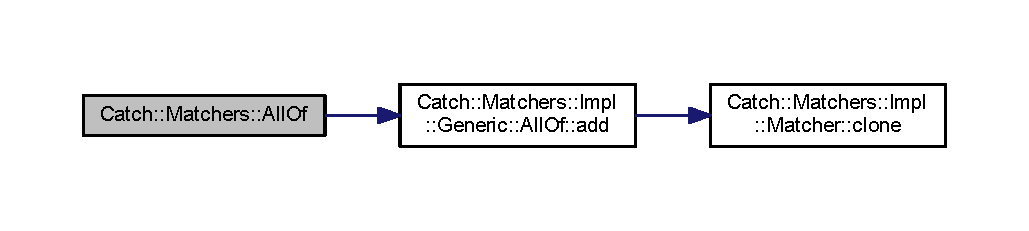
\includegraphics[width=350pt]{namespace_catch_1_1_matchers_aca6c1c17e137d989583c97f99705797a_cgraph}
\end{center}
\end{figure}
\hypertarget{namespace_catch_1_1_matchers_a990366f7d62d10d9752ad7b24230def0}{}\label{namespace_catch_1_1_matchers_a990366f7d62d10d9752ad7b24230def0} 
\index{Catch\+::\+Matchers@{Catch\+::\+Matchers}!All\+Of@{All\+Of}}
\index{All\+Of@{All\+Of}!Catch\+::\+Matchers@{Catch\+::\+Matchers}}
\subsubsection{\texorpdfstring{All\+Of()}{AllOf()}\hspace{0.1cm}{\footnotesize\ttfamily [2/2]}}
{\footnotesize\ttfamily template$<$typename ExpressionT $>$ \\
\hyperlink{class_catch_1_1_matchers_1_1_impl_1_1_generic_1_1_all_of}{Impl\+::\+Generic\+::\+All\+Of}$<$ExpressionT$>$ Catch\+::\+Matchers\+::\+All\+Of (\begin{DoxyParamCaption}\item[{\hyperlink{struct_catch_1_1_matchers_1_1_impl_1_1_matcher}{Impl\+::\+Matcher}$<$ ExpressionT $>$ const \&}]{m1,  }\item[{\hyperlink{struct_catch_1_1_matchers_1_1_impl_1_1_matcher}{Impl\+::\+Matcher}$<$ ExpressionT $>$ const \&}]{m2,  }\item[{\hyperlink{struct_catch_1_1_matchers_1_1_impl_1_1_matcher}{Impl\+::\+Matcher}$<$ ExpressionT $>$ const \&}]{m3 }\end{DoxyParamCaption})\hspace{0.3cm}{\ttfamily [inline]}}



Definition at line 1159 of file catch.\+hpp.

Here is the call graph for this function\+:\nopagebreak
\begin{figure}[H]
\begin{center}
\leavevmode
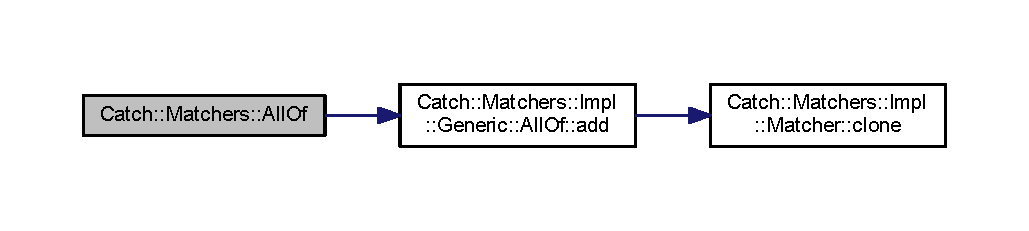
\includegraphics[width=350pt]{namespace_catch_1_1_matchers_a990366f7d62d10d9752ad7b24230def0_cgraph}
\end{center}
\end{figure}
\hypertarget{namespace_catch_1_1_matchers_a9cb139c71b9e391d5fc017764695bf84}{}\label{namespace_catch_1_1_matchers_a9cb139c71b9e391d5fc017764695bf84} 
\index{Catch\+::\+Matchers@{Catch\+::\+Matchers}!Any\+Of@{Any\+Of}}
\index{Any\+Of@{Any\+Of}!Catch\+::\+Matchers@{Catch\+::\+Matchers}}
\subsubsection{\texorpdfstring{Any\+Of()}{AnyOf()}\hspace{0.1cm}{\footnotesize\ttfamily [1/2]}}
{\footnotesize\ttfamily template$<$typename ExpressionT $>$ \\
\hyperlink{class_catch_1_1_matchers_1_1_impl_1_1_generic_1_1_any_of}{Impl\+::\+Generic\+::\+Any\+Of}$<$ExpressionT$>$ Catch\+::\+Matchers\+::\+Any\+Of (\begin{DoxyParamCaption}\item[{\hyperlink{struct_catch_1_1_matchers_1_1_impl_1_1_matcher}{Impl\+::\+Matcher}$<$ ExpressionT $>$ const \&}]{m1,  }\item[{\hyperlink{struct_catch_1_1_matchers_1_1_impl_1_1_matcher}{Impl\+::\+Matcher}$<$ ExpressionT $>$ const \&}]{m2 }\end{DoxyParamCaption})\hspace{0.3cm}{\ttfamily [inline]}}



Definition at line 1165 of file catch.\+hpp.

Here is the call graph for this function\+:\nopagebreak
\begin{figure}[H]
\begin{center}
\leavevmode
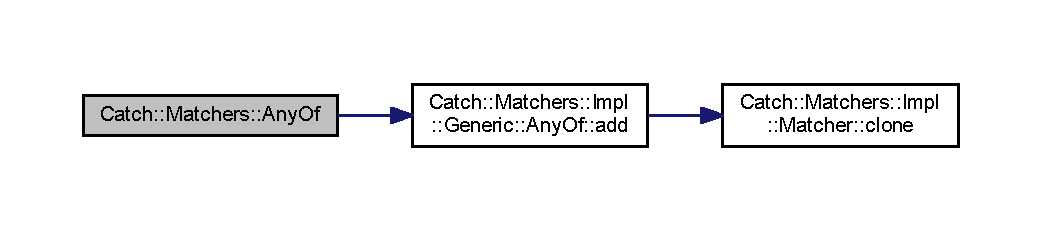
\includegraphics[width=350pt]{namespace_catch_1_1_matchers_a9cb139c71b9e391d5fc017764695bf84_cgraph}
\end{center}
\end{figure}
\hypertarget{namespace_catch_1_1_matchers_a8efb0e533db973b8aff1172fb908db02}{}\label{namespace_catch_1_1_matchers_a8efb0e533db973b8aff1172fb908db02} 
\index{Catch\+::\+Matchers@{Catch\+::\+Matchers}!Any\+Of@{Any\+Of}}
\index{Any\+Of@{Any\+Of}!Catch\+::\+Matchers@{Catch\+::\+Matchers}}
\subsubsection{\texorpdfstring{Any\+Of()}{AnyOf()}\hspace{0.1cm}{\footnotesize\ttfamily [2/2]}}
{\footnotesize\ttfamily template$<$typename ExpressionT $>$ \\
\hyperlink{class_catch_1_1_matchers_1_1_impl_1_1_generic_1_1_any_of}{Impl\+::\+Generic\+::\+Any\+Of}$<$ExpressionT$>$ Catch\+::\+Matchers\+::\+Any\+Of (\begin{DoxyParamCaption}\item[{\hyperlink{struct_catch_1_1_matchers_1_1_impl_1_1_matcher}{Impl\+::\+Matcher}$<$ ExpressionT $>$ const \&}]{m1,  }\item[{\hyperlink{struct_catch_1_1_matchers_1_1_impl_1_1_matcher}{Impl\+::\+Matcher}$<$ ExpressionT $>$ const \&}]{m2,  }\item[{\hyperlink{struct_catch_1_1_matchers_1_1_impl_1_1_matcher}{Impl\+::\+Matcher}$<$ ExpressionT $>$ const \&}]{m3 }\end{DoxyParamCaption})\hspace{0.3cm}{\ttfamily [inline]}}



Definition at line 1170 of file catch.\+hpp.

Here is the call graph for this function\+:\nopagebreak
\begin{figure}[H]
\begin{center}
\leavevmode
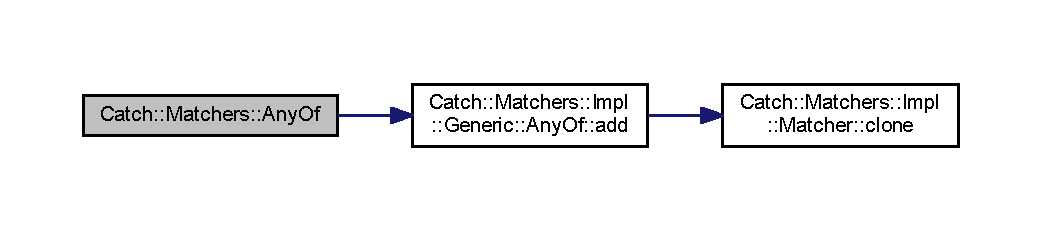
\includegraphics[width=350pt]{namespace_catch_1_1_matchers_a8efb0e533db973b8aff1172fb908db02_cgraph}
\end{center}
\end{figure}
\hypertarget{namespace_catch_1_1_matchers_a07760045eca8bafb7f6618fae10f1b59}{}\label{namespace_catch_1_1_matchers_a07760045eca8bafb7f6618fae10f1b59} 
\index{Catch\+::\+Matchers@{Catch\+::\+Matchers}!Contains@{Contains}}
\index{Contains@{Contains}!Catch\+::\+Matchers@{Catch\+::\+Matchers}}
\subsubsection{\texorpdfstring{Contains()}{Contains()}\hspace{0.1cm}{\footnotesize\ttfamily [1/2]}}
{\footnotesize\ttfamily \hyperlink{struct_catch_1_1_matchers_1_1_impl_1_1_std_string_1_1_contains}{Impl\+::\+Std\+String\+::\+Contains} Catch\+::\+Matchers\+::\+Contains (\begin{DoxyParamCaption}\item[{std\+::string const \&}]{substr,  }\item[{\hyperlink{struct_catch_1_1_case_sensitive_aad49d3aee2d97066642fffa919685c6a}{Case\+Sensitive\+::\+Choice}}]{case\+Sensitivity = {\ttfamily \hyperlink{struct_catch_1_1_case_sensitive_aad49d3aee2d97066642fffa919685c6aa7c5550b69ec3c502e6f609b67f9613c6}{Case\+Sensitive\+::\+Yes}} }\end{DoxyParamCaption})\hspace{0.3cm}{\ttfamily [inline]}}



Definition at line 1182 of file catch.\+hpp.

Here is the call graph for this function\+:\nopagebreak
\begin{figure}[H]
\begin{center}
\leavevmode
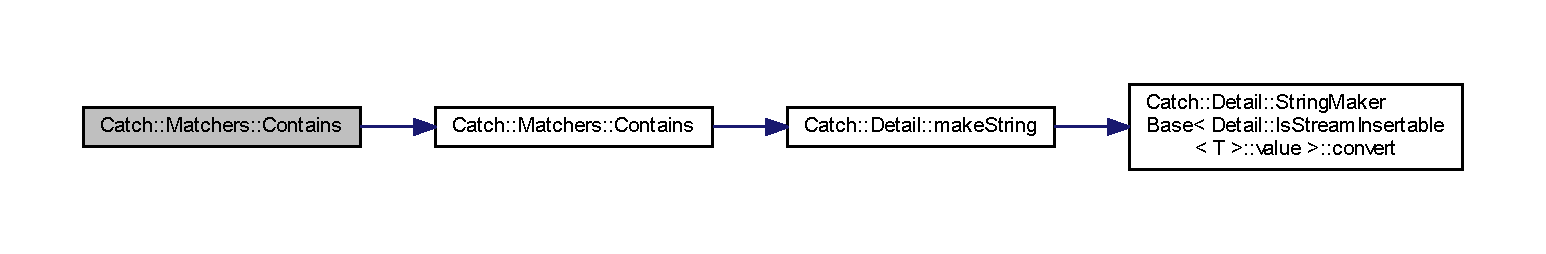
\includegraphics[width=350pt]{namespace_catch_1_1_matchers_a07760045eca8bafb7f6618fae10f1b59_cgraph}
\end{center}
\end{figure}
\hypertarget{namespace_catch_1_1_matchers_a7bc27b5c696118cbe54690d6c524b3d9}{}\label{namespace_catch_1_1_matchers_a7bc27b5c696118cbe54690d6c524b3d9} 
\index{Catch\+::\+Matchers@{Catch\+::\+Matchers}!Contains@{Contains}}
\index{Contains@{Contains}!Catch\+::\+Matchers@{Catch\+::\+Matchers}}
\subsubsection{\texorpdfstring{Contains()}{Contains()}\hspace{0.1cm}{\footnotesize\ttfamily [2/2]}}
{\footnotesize\ttfamily \hyperlink{struct_catch_1_1_matchers_1_1_impl_1_1_std_string_1_1_contains}{Impl\+::\+Std\+String\+::\+Contains} Catch\+::\+Matchers\+::\+Contains (\begin{DoxyParamCaption}\item[{const char $\ast$}]{substr,  }\item[{\hyperlink{struct_catch_1_1_case_sensitive_aad49d3aee2d97066642fffa919685c6a}{Case\+Sensitive\+::\+Choice}}]{case\+Sensitivity = {\ttfamily \hyperlink{struct_catch_1_1_case_sensitive_aad49d3aee2d97066642fffa919685c6aa7c5550b69ec3c502e6f609b67f9613c6}{Case\+Sensitive\+::\+Yes}} }\end{DoxyParamCaption})\hspace{0.3cm}{\ttfamily [inline]}}



Definition at line 1185 of file catch.\+hpp.

Here is the call graph for this function\+:\nopagebreak
\begin{figure}[H]
\begin{center}
\leavevmode
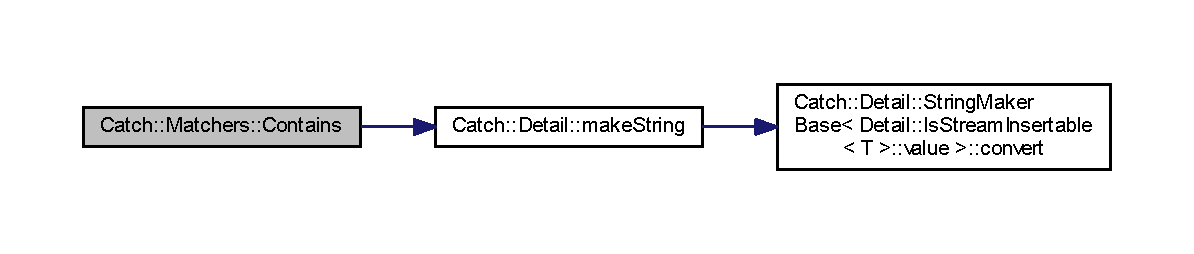
\includegraphics[width=350pt]{namespace_catch_1_1_matchers_a7bc27b5c696118cbe54690d6c524b3d9_cgraph}
\end{center}
\end{figure}
Here is the caller graph for this function\+:\nopagebreak
\begin{figure}[H]
\begin{center}
\leavevmode
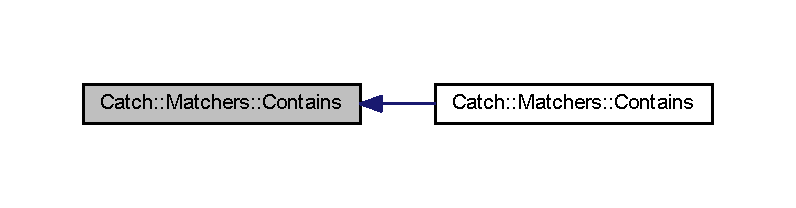
\includegraphics[width=350pt]{namespace_catch_1_1_matchers_a7bc27b5c696118cbe54690d6c524b3d9_icgraph}
\end{center}
\end{figure}
\hypertarget{namespace_catch_1_1_matchers_a1e32a2d23a1eb9eda9840c712c7b00c1}{}\label{namespace_catch_1_1_matchers_a1e32a2d23a1eb9eda9840c712c7b00c1} 
\index{Catch\+::\+Matchers@{Catch\+::\+Matchers}!Ends\+With@{Ends\+With}}
\index{Ends\+With@{Ends\+With}!Catch\+::\+Matchers@{Catch\+::\+Matchers}}
\subsubsection{\texorpdfstring{Ends\+With()}{EndsWith()}\hspace{0.1cm}{\footnotesize\ttfamily [1/2]}}
{\footnotesize\ttfamily \hyperlink{struct_catch_1_1_matchers_1_1_impl_1_1_std_string_1_1_ends_with}{Impl\+::\+Std\+String\+::\+Ends\+With} Catch\+::\+Matchers\+::\+Ends\+With (\begin{DoxyParamCaption}\item[{std\+::string const \&}]{substr }\end{DoxyParamCaption})\hspace{0.3cm}{\ttfamily [inline]}}



Definition at line 1194 of file catch.\+hpp.

Here is the call graph for this function\+:\nopagebreak
\begin{figure}[H]
\begin{center}
\leavevmode
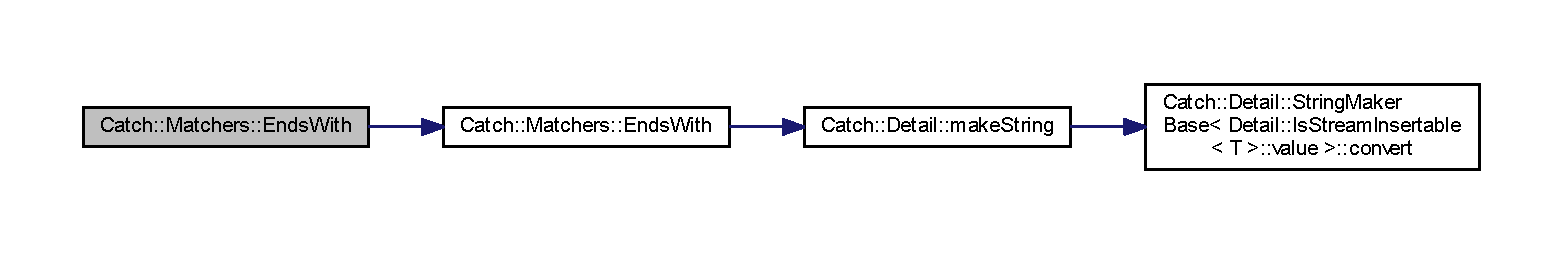
\includegraphics[width=350pt]{namespace_catch_1_1_matchers_a1e32a2d23a1eb9eda9840c712c7b00c1_cgraph}
\end{center}
\end{figure}
\hypertarget{namespace_catch_1_1_matchers_ae3e6d8f7fea6fac6513596b23e5d5153}{}\label{namespace_catch_1_1_matchers_ae3e6d8f7fea6fac6513596b23e5d5153} 
\index{Catch\+::\+Matchers@{Catch\+::\+Matchers}!Ends\+With@{Ends\+With}}
\index{Ends\+With@{Ends\+With}!Catch\+::\+Matchers@{Catch\+::\+Matchers}}
\subsubsection{\texorpdfstring{Ends\+With()}{EndsWith()}\hspace{0.1cm}{\footnotesize\ttfamily [2/2]}}
{\footnotesize\ttfamily \hyperlink{struct_catch_1_1_matchers_1_1_impl_1_1_std_string_1_1_ends_with}{Impl\+::\+Std\+String\+::\+Ends\+With} Catch\+::\+Matchers\+::\+Ends\+With (\begin{DoxyParamCaption}\item[{const char $\ast$}]{substr }\end{DoxyParamCaption})\hspace{0.3cm}{\ttfamily [inline]}}



Definition at line 1197 of file catch.\+hpp.

Here is the call graph for this function\+:\nopagebreak
\begin{figure}[H]
\begin{center}
\leavevmode
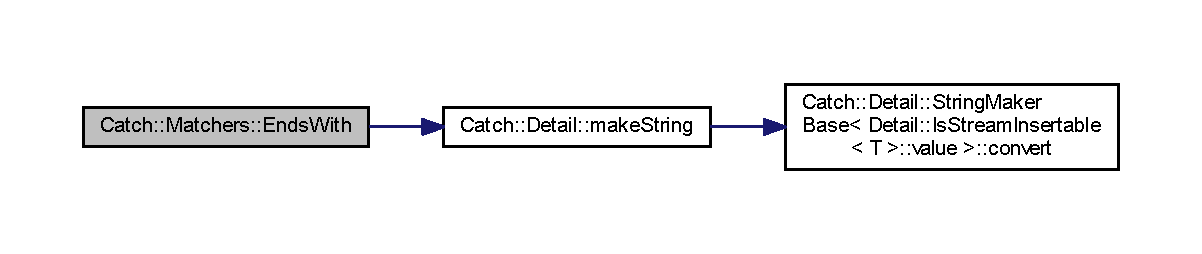
\includegraphics[width=350pt]{namespace_catch_1_1_matchers_ae3e6d8f7fea6fac6513596b23e5d5153_cgraph}
\end{center}
\end{figure}
Here is the caller graph for this function\+:\nopagebreak
\begin{figure}[H]
\begin{center}
\leavevmode
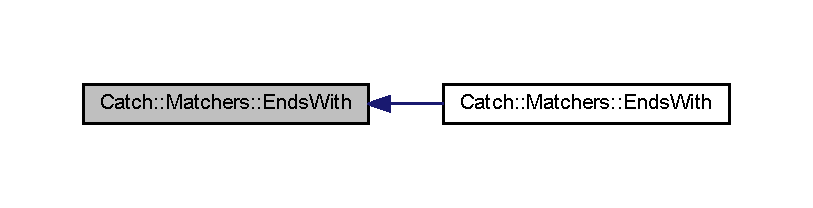
\includegraphics[width=350pt]{namespace_catch_1_1_matchers_ae3e6d8f7fea6fac6513596b23e5d5153_icgraph}
\end{center}
\end{figure}
\hypertarget{namespace_catch_1_1_matchers_a840317a3d0f828642c2f55155068bb97}{}\label{namespace_catch_1_1_matchers_a840317a3d0f828642c2f55155068bb97} 
\index{Catch\+::\+Matchers@{Catch\+::\+Matchers}!Equals@{Equals}}
\index{Equals@{Equals}!Catch\+::\+Matchers@{Catch\+::\+Matchers}}
\subsubsection{\texorpdfstring{Equals()}{Equals()}\hspace{0.1cm}{\footnotesize\ttfamily [1/2]}}
{\footnotesize\ttfamily \hyperlink{struct_catch_1_1_matchers_1_1_impl_1_1_std_string_1_1_equals}{Impl\+::\+Std\+String\+::\+Equals} Catch\+::\+Matchers\+::\+Equals (\begin{DoxyParamCaption}\item[{std\+::string const \&}]{str,  }\item[{\hyperlink{struct_catch_1_1_case_sensitive_aad49d3aee2d97066642fffa919685c6a}{Case\+Sensitive\+::\+Choice}}]{case\+Sensitivity = {\ttfamily \hyperlink{struct_catch_1_1_case_sensitive_aad49d3aee2d97066642fffa919685c6aa7c5550b69ec3c502e6f609b67f9613c6}{Case\+Sensitive\+::\+Yes}} }\end{DoxyParamCaption})\hspace{0.3cm}{\ttfamily [inline]}}



Definition at line 1176 of file catch.\+hpp.

Here is the call graph for this function\+:\nopagebreak
\begin{figure}[H]
\begin{center}
\leavevmode
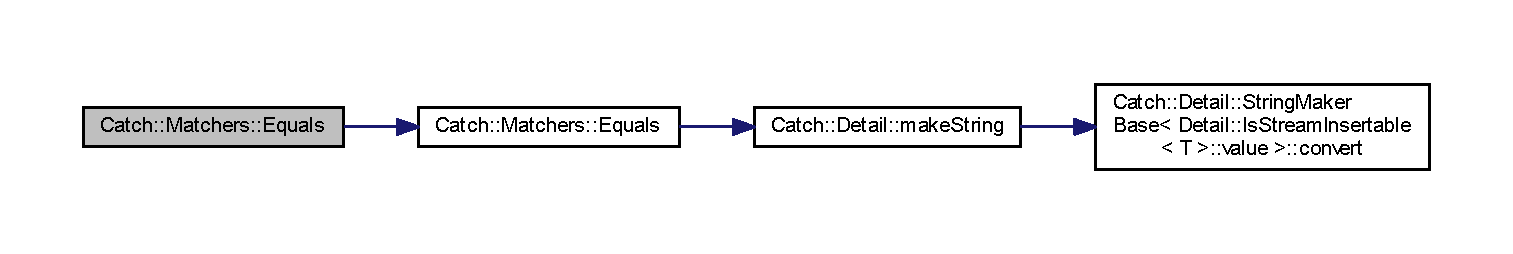
\includegraphics[width=350pt]{namespace_catch_1_1_matchers_a840317a3d0f828642c2f55155068bb97_cgraph}
\end{center}
\end{figure}
\hypertarget{namespace_catch_1_1_matchers_a7454444261cc4af7ee0b0bc82cf74284}{}\label{namespace_catch_1_1_matchers_a7454444261cc4af7ee0b0bc82cf74284} 
\index{Catch\+::\+Matchers@{Catch\+::\+Matchers}!Equals@{Equals}}
\index{Equals@{Equals}!Catch\+::\+Matchers@{Catch\+::\+Matchers}}
\subsubsection{\texorpdfstring{Equals()}{Equals()}\hspace{0.1cm}{\footnotesize\ttfamily [2/2]}}
{\footnotesize\ttfamily \hyperlink{struct_catch_1_1_matchers_1_1_impl_1_1_std_string_1_1_equals}{Impl\+::\+Std\+String\+::\+Equals} Catch\+::\+Matchers\+::\+Equals (\begin{DoxyParamCaption}\item[{const char $\ast$}]{str,  }\item[{\hyperlink{struct_catch_1_1_case_sensitive_aad49d3aee2d97066642fffa919685c6a}{Case\+Sensitive\+::\+Choice}}]{case\+Sensitivity = {\ttfamily \hyperlink{struct_catch_1_1_case_sensitive_aad49d3aee2d97066642fffa919685c6aa7c5550b69ec3c502e6f609b67f9613c6}{Case\+Sensitive\+::\+Yes}} }\end{DoxyParamCaption})\hspace{0.3cm}{\ttfamily [inline]}}



Definition at line 1179 of file catch.\+hpp.

Here is the call graph for this function\+:\nopagebreak
\begin{figure}[H]
\begin{center}
\leavevmode
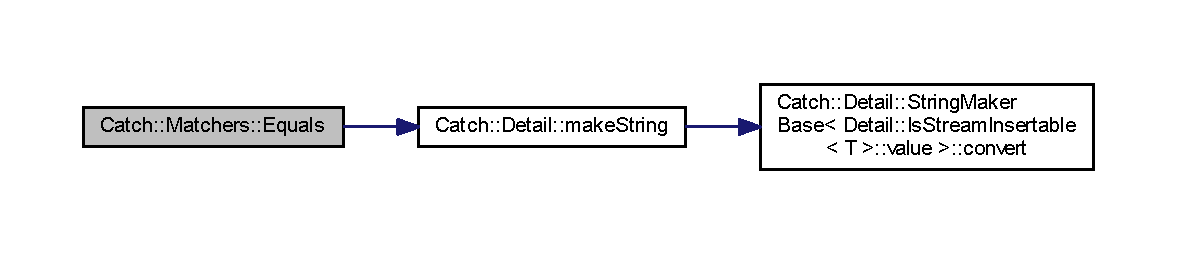
\includegraphics[width=350pt]{namespace_catch_1_1_matchers_a7454444261cc4af7ee0b0bc82cf74284_cgraph}
\end{center}
\end{figure}
Here is the caller graph for this function\+:\nopagebreak
\begin{figure}[H]
\begin{center}
\leavevmode
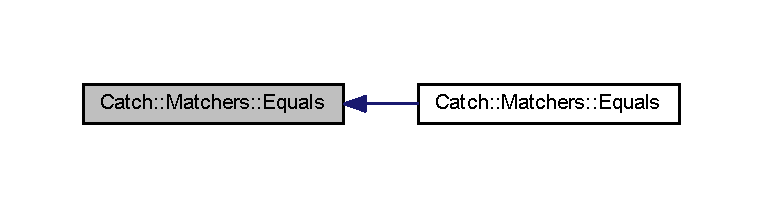
\includegraphics[width=350pt]{namespace_catch_1_1_matchers_a7454444261cc4af7ee0b0bc82cf74284_icgraph}
\end{center}
\end{figure}
\hypertarget{namespace_catch_1_1_matchers_ae3c192dc15c973c38f07376d4debdc34}{}\label{namespace_catch_1_1_matchers_ae3c192dc15c973c38f07376d4debdc34} 
\index{Catch\+::\+Matchers@{Catch\+::\+Matchers}!Not@{Not}}
\index{Not@{Not}!Catch\+::\+Matchers@{Catch\+::\+Matchers}}
\subsubsection{\texorpdfstring{Not()}{Not()}}
{\footnotesize\ttfamily template$<$typename ExpressionT $>$ \\
\hyperlink{class_catch_1_1_matchers_1_1_impl_1_1_generic_1_1_not}{Impl\+::\+Generic\+::\+Not}$<$ExpressionT$>$ Catch\+::\+Matchers\+::\+Not (\begin{DoxyParamCaption}\item[{\hyperlink{struct_catch_1_1_matchers_1_1_impl_1_1_matcher}{Impl\+::\+Matcher}$<$ ExpressionT $>$ const \&}]{m }\end{DoxyParamCaption})\hspace{0.3cm}{\ttfamily [inline]}}



Definition at line 1149 of file catch.\+hpp.

Here is the caller graph for this function\+:\nopagebreak
\begin{figure}[H]
\begin{center}
\leavevmode
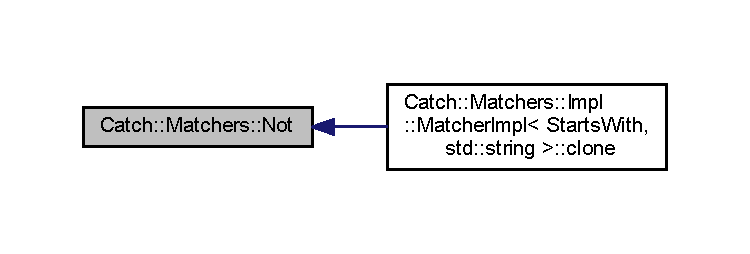
\includegraphics[width=350pt]{namespace_catch_1_1_matchers_ae3c192dc15c973c38f07376d4debdc34_icgraph}
\end{center}
\end{figure}
\hypertarget{namespace_catch_1_1_matchers_a9b6a7704df7d0717dc6686fd2055ffea}{}\label{namespace_catch_1_1_matchers_a9b6a7704df7d0717dc6686fd2055ffea} 
\index{Catch\+::\+Matchers@{Catch\+::\+Matchers}!Starts\+With@{Starts\+With}}
\index{Starts\+With@{Starts\+With}!Catch\+::\+Matchers@{Catch\+::\+Matchers}}
\subsubsection{\texorpdfstring{Starts\+With()}{StartsWith()}\hspace{0.1cm}{\footnotesize\ttfamily [1/2]}}
{\footnotesize\ttfamily \hyperlink{struct_catch_1_1_matchers_1_1_impl_1_1_std_string_1_1_starts_with}{Impl\+::\+Std\+String\+::\+Starts\+With} Catch\+::\+Matchers\+::\+Starts\+With (\begin{DoxyParamCaption}\item[{std\+::string const \&}]{substr }\end{DoxyParamCaption})\hspace{0.3cm}{\ttfamily [inline]}}



Definition at line 1188 of file catch.\+hpp.

Here is the call graph for this function\+:\nopagebreak
\begin{figure}[H]
\begin{center}
\leavevmode
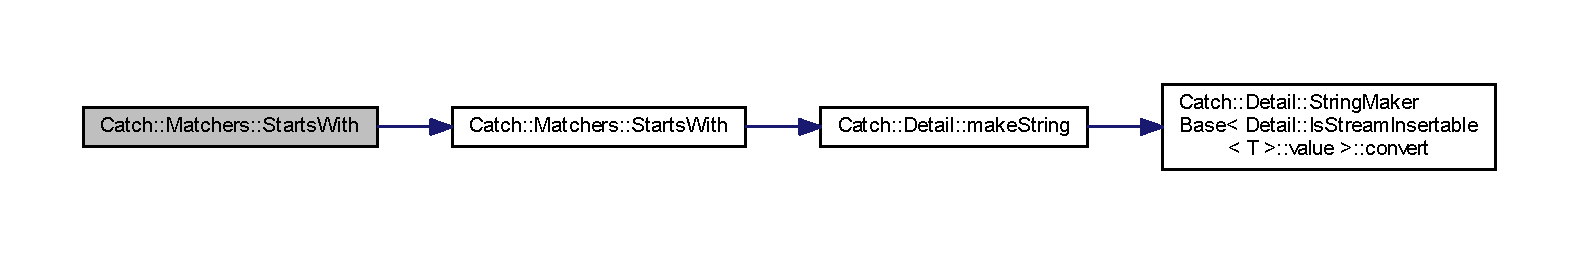
\includegraphics[width=350pt]{namespace_catch_1_1_matchers_a9b6a7704df7d0717dc6686fd2055ffea_cgraph}
\end{center}
\end{figure}
\hypertarget{namespace_catch_1_1_matchers_a031985c11b8c8bb62585b3904f9fd2b0}{}\label{namespace_catch_1_1_matchers_a031985c11b8c8bb62585b3904f9fd2b0} 
\index{Catch\+::\+Matchers@{Catch\+::\+Matchers}!Starts\+With@{Starts\+With}}
\index{Starts\+With@{Starts\+With}!Catch\+::\+Matchers@{Catch\+::\+Matchers}}
\subsubsection{\texorpdfstring{Starts\+With()}{StartsWith()}\hspace{0.1cm}{\footnotesize\ttfamily [2/2]}}
{\footnotesize\ttfamily \hyperlink{struct_catch_1_1_matchers_1_1_impl_1_1_std_string_1_1_starts_with}{Impl\+::\+Std\+String\+::\+Starts\+With} Catch\+::\+Matchers\+::\+Starts\+With (\begin{DoxyParamCaption}\item[{const char $\ast$}]{substr }\end{DoxyParamCaption})\hspace{0.3cm}{\ttfamily [inline]}}



Definition at line 1191 of file catch.\+hpp.

Here is the call graph for this function\+:\nopagebreak
\begin{figure}[H]
\begin{center}
\leavevmode
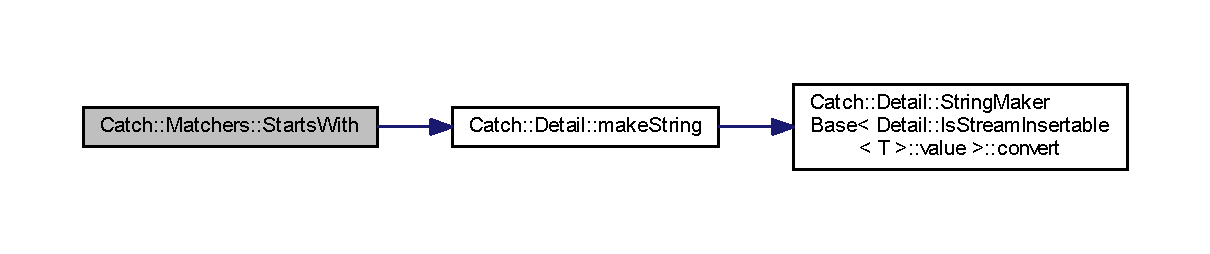
\includegraphics[width=350pt]{namespace_catch_1_1_matchers_a031985c11b8c8bb62585b3904f9fd2b0_cgraph}
\end{center}
\end{figure}
Here is the caller graph for this function\+:\nopagebreak
\begin{figure}[H]
\begin{center}
\leavevmode
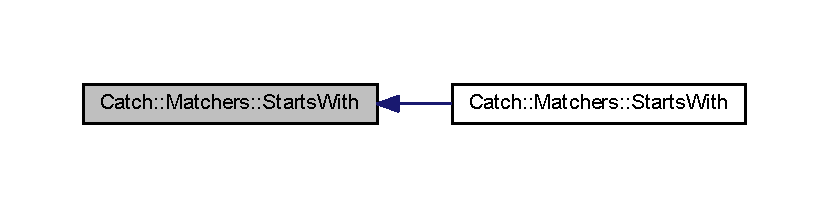
\includegraphics[width=350pt]{namespace_catch_1_1_matchers_a031985c11b8c8bb62585b3904f9fd2b0_icgraph}
\end{center}
\end{figure}

\hypertarget{namespace_catch_1_1_matchers_1_1_impl}{}\section{Catch\+:\+:Matchers\+:\+:Impl Namespace Reference}
\label{namespace_catch_1_1_matchers_1_1_impl}\index{Catch\+::\+Matchers\+::\+Impl@{Catch\+::\+Matchers\+::\+Impl}}
\subsection*{Namespaces}
\begin{DoxyCompactItemize}
\item 
 \hyperlink{namespace_catch_1_1_matchers_1_1_impl_1_1_generic}{Generic}
\item 
 \hyperlink{namespace_catch_1_1_matchers_1_1_impl_1_1_std_string}{Std\+String}
\end{DoxyCompactItemize}
\subsection*{Classes}
\begin{DoxyCompactItemize}
\item 
struct \hyperlink{struct_catch_1_1_matchers_1_1_impl_1_1_matcher}{Matcher}
\item 
struct \hyperlink{struct_catch_1_1_matchers_1_1_impl_1_1_matcher_impl}{Matcher\+Impl}
\end{DoxyCompactItemize}

\hypertarget{namespace_catch_1_1_matchers_1_1_impl_1_1_generic}{}\section{Catch\+:\+:Matchers\+:\+:Impl\+:\+:Generic Namespace Reference}
\label{namespace_catch_1_1_matchers_1_1_impl_1_1_generic}\index{Catch\+::\+Matchers\+::\+Impl\+::\+Generic@{Catch\+::\+Matchers\+::\+Impl\+::\+Generic}}
\subsection*{Classes}
\begin{DoxyCompactItemize}
\item 
class \hyperlink{class_catch_1_1_matchers_1_1_impl_1_1_generic_1_1_all_of}{All\+Of}
\item 
class \hyperlink{class_catch_1_1_matchers_1_1_impl_1_1_generic_1_1_any_of}{Any\+Of}
\item 
class \hyperlink{class_catch_1_1_matchers_1_1_impl_1_1_generic_1_1_not}{Not}
\end{DoxyCompactItemize}

\hypertarget{namespace_catch_1_1_matchers_1_1_impl_1_1_std_string}{}\section{Catch\+:\+:Matchers\+:\+:Impl\+:\+:Std\+String Namespace Reference}
\label{namespace_catch_1_1_matchers_1_1_impl_1_1_std_string}\index{Catch\+::\+Matchers\+::\+Impl\+::\+Std\+String@{Catch\+::\+Matchers\+::\+Impl\+::\+Std\+String}}
\subsection*{Classes}
\begin{DoxyCompactItemize}
\item 
struct \hyperlink{struct_catch_1_1_matchers_1_1_impl_1_1_std_string_1_1_cased_string}{Cased\+String}
\item 
struct \hyperlink{struct_catch_1_1_matchers_1_1_impl_1_1_std_string_1_1_contains}{Contains}
\item 
struct \hyperlink{struct_catch_1_1_matchers_1_1_impl_1_1_std_string_1_1_ends_with}{Ends\+With}
\item 
struct \hyperlink{struct_catch_1_1_matchers_1_1_impl_1_1_std_string_1_1_equals}{Equals}
\item 
struct \hyperlink{struct_catch_1_1_matchers_1_1_impl_1_1_std_string_1_1_starts_with}{Starts\+With}
\end{DoxyCompactItemize}
\subsection*{Functions}
\begin{DoxyCompactItemize}
\item 
std\+::string \hyperlink{namespace_catch_1_1_matchers_1_1_impl_1_1_std_string_a1c41960bd2b455975e7be3cb87878fef}{make\+String} (std\+::string const \&str)
\item 
std\+::string \hyperlink{namespace_catch_1_1_matchers_1_1_impl_1_1_std_string_a42a104fb88baf158ed3b7d0d422afdaa}{make\+String} (const char $\ast$str)
\end{DoxyCompactItemize}


\subsection{Function Documentation}
\hypertarget{namespace_catch_1_1_matchers_1_1_impl_1_1_std_string_a1c41960bd2b455975e7be3cb87878fef}{}\label{namespace_catch_1_1_matchers_1_1_impl_1_1_std_string_a1c41960bd2b455975e7be3cb87878fef} 
\index{Catch\+::\+Matchers\+::\+Impl\+::\+Std\+String@{Catch\+::\+Matchers\+::\+Impl\+::\+Std\+String}!make\+String@{make\+String}}
\index{make\+String@{make\+String}!Catch\+::\+Matchers\+::\+Impl\+::\+Std\+String@{Catch\+::\+Matchers\+::\+Impl\+::\+Std\+String}}
\subsubsection{\texorpdfstring{make\+String()}{makeString()}\hspace{0.1cm}{\footnotesize\ttfamily [1/2]}}
{\footnotesize\ttfamily std\+::string Catch\+::\+Matchers\+::\+Impl\+::\+Std\+String\+::make\+String (\begin{DoxyParamCaption}\item[{std\+::string const \&}]{str }\end{DoxyParamCaption})\hspace{0.3cm}{\ttfamily [inline]}}



Definition at line 1049 of file catch.\+hpp.

\hypertarget{namespace_catch_1_1_matchers_1_1_impl_1_1_std_string_a42a104fb88baf158ed3b7d0d422afdaa}{}\label{namespace_catch_1_1_matchers_1_1_impl_1_1_std_string_a42a104fb88baf158ed3b7d0d422afdaa} 
\index{Catch\+::\+Matchers\+::\+Impl\+::\+Std\+String@{Catch\+::\+Matchers\+::\+Impl\+::\+Std\+String}!make\+String@{make\+String}}
\index{make\+String@{make\+String}!Catch\+::\+Matchers\+::\+Impl\+::\+Std\+String@{Catch\+::\+Matchers\+::\+Impl\+::\+Std\+String}}
\subsubsection{\texorpdfstring{make\+String()}{makeString()}\hspace{0.1cm}{\footnotesize\ttfamily [2/2]}}
{\footnotesize\ttfamily std\+::string Catch\+::\+Matchers\+::\+Impl\+::\+Std\+String\+::make\+String (\begin{DoxyParamCaption}\item[{const char $\ast$}]{str }\end{DoxyParamCaption})\hspace{0.3cm}{\ttfamily [inline]}}



Definition at line 1050 of file catch.\+hpp.


\chapter{Class Documentation}
\hypertarget{classafficheur}{}\section{afficheur Class Reference}
\label{classafficheur}\index{afficheur@{afficheur}}


{\ttfamily \#include $<$afficheur.\+h$>$}



Inheritance diagram for afficheur\+:\nopagebreak
\begin{figure}[H]
\begin{center}
\leavevmode
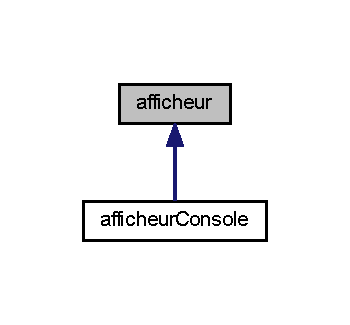
\includegraphics[width=168pt]{classafficheur__inherit__graph}
\end{center}
\end{figure}
\subsection*{Public Member Functions}
\begin{DoxyCompactItemize}
\item 
\hyperlink{classafficheur_a6bc02ed7b0dbbb21607528ae03c4f886}{afficheur} ()=default
\item 
virtual \hyperlink{classafficheur_a093c44d15f6de24883abce836bfd11c9}{$\sim$afficheur} ()
\begin{DoxyCompactList}\small\item\em Destructeur virtuel de l\textquotesingle{}objet afficheur. \end{DoxyCompactList}\item 
virtual void \hyperlink{classafficheur_a1551534b5916a48d3ea73f0d68929e95}{affiche\+Semaine} (const \hyperlink{classhoraire}{horaire} $\ast$h, ostream \&ost)=0
\item 
virtual void \hyperlink{classafficheur_a3c3ace0f2f01e95a1cc86a0b6c497e34}{affiche\+Heure} (const \hyperlink{classhoraire}{horaire} $\ast$h, ostream \&ost)=0
\item 
virtual void \hyperlink{classafficheur_a0cea335dad556ceba3487ae261b831f9}{affiche\+Jour} (const \hyperlink{classhoraire}{horaire} $\ast$h, ostream \&ost)=0
\item 
virtual void \hyperlink{classafficheur_aa598626f11775b4c610b8f262017cad7}{affiche\+Horaire} (const \hyperlink{classhoraire}{horaire} $\ast$h, ostream \&ost)=0
\item 
virtual void \hyperlink{classafficheur_a54b3e457d56738ed20641e5546872142}{affiche\+Professeur} (const \hyperlink{classprofesseur}{professeur} $\ast$p, ostream \&ost)=0
\item 
virtual void \hyperlink{classafficheur_af8b1bc89ba8c0f2acdd9a78f97a2949f}{affiche\+Salle} (const \hyperlink{classsalle}{salle} $\ast$s, ostream \&ost)=0
\item 
virtual void \hyperlink{classafficheur_a9d176576ad45c2a07a8a887b853b7edb}{affiche\+Cours} (const \hyperlink{classcours}{cours} $\ast$c, ostream \&ost)=0
\end{DoxyCompactItemize}


\subsection{Detailed Description}


Definition at line 20 of file afficheur.\+h.



\subsection{Constructor \& Destructor Documentation}
\hypertarget{classafficheur_a6bc02ed7b0dbbb21607528ae03c4f886}{}\label{classafficheur_a6bc02ed7b0dbbb21607528ae03c4f886} 
\index{afficheur@{afficheur}!afficheur@{afficheur}}
\index{afficheur@{afficheur}!afficheur@{afficheur}}
\subsubsection{\texorpdfstring{afficheur()}{afficheur()}}
{\footnotesize\ttfamily afficheur\+::afficheur (\begin{DoxyParamCaption}{ }\end{DoxyParamCaption})\hspace{0.3cm}{\ttfamily [default]}}

\hypertarget{classafficheur_a093c44d15f6de24883abce836bfd11c9}{}\label{classafficheur_a093c44d15f6de24883abce836bfd11c9} 
\index{afficheur@{afficheur}!````~afficheur@{$\sim$afficheur}}
\index{````~afficheur@{$\sim$afficheur}!afficheur@{afficheur}}
\subsubsection{\texorpdfstring{$\sim$afficheur()}{~afficheur()}}
{\footnotesize\ttfamily afficheur\+::$\sim$afficheur (\begin{DoxyParamCaption}{ }\end{DoxyParamCaption})\hspace{0.3cm}{\ttfamily [virtual]}}



Destructeur virtuel de l\textquotesingle{}objet afficheur. 



Definition at line 14 of file afficheur.\+cpp.



\subsection{Member Function Documentation}
\hypertarget{classafficheur_a9d176576ad45c2a07a8a887b853b7edb}{}\label{classafficheur_a9d176576ad45c2a07a8a887b853b7edb} 
\index{afficheur@{afficheur}!affiche\+Cours@{affiche\+Cours}}
\index{affiche\+Cours@{affiche\+Cours}!afficheur@{afficheur}}
\subsubsection{\texorpdfstring{affiche\+Cours()}{afficheCours()}}
{\footnotesize\ttfamily virtual void afficheur\+::affiche\+Cours (\begin{DoxyParamCaption}\item[{const \hyperlink{classcours}{cours} $\ast$}]{c,  }\item[{ostream \&}]{ost }\end{DoxyParamCaption})\hspace{0.3cm}{\ttfamily [pure virtual]}}



Implemented in \hyperlink{classafficheur_console_aa77bdd8065edd5269f83679490e78dee}{afficheur\+Console}.

\hypertarget{classafficheur_a3c3ace0f2f01e95a1cc86a0b6c497e34}{}\label{classafficheur_a3c3ace0f2f01e95a1cc86a0b6c497e34} 
\index{afficheur@{afficheur}!affiche\+Heure@{affiche\+Heure}}
\index{affiche\+Heure@{affiche\+Heure}!afficheur@{afficheur}}
\subsubsection{\texorpdfstring{affiche\+Heure()}{afficheHeure()}}
{\footnotesize\ttfamily virtual void afficheur\+::affiche\+Heure (\begin{DoxyParamCaption}\item[{const \hyperlink{classhoraire}{horaire} $\ast$}]{h,  }\item[{ostream \&}]{ost }\end{DoxyParamCaption})\hspace{0.3cm}{\ttfamily [pure virtual]}}



Implemented in \hyperlink{classafficheur_console_a842884a9553df737f781d2f8f040d30e}{afficheur\+Console}.

\hypertarget{classafficheur_aa598626f11775b4c610b8f262017cad7}{}\label{classafficheur_aa598626f11775b4c610b8f262017cad7} 
\index{afficheur@{afficheur}!affiche\+Horaire@{affiche\+Horaire}}
\index{affiche\+Horaire@{affiche\+Horaire}!afficheur@{afficheur}}
\subsubsection{\texorpdfstring{affiche\+Horaire()}{afficheHoraire()}}
{\footnotesize\ttfamily virtual void afficheur\+::affiche\+Horaire (\begin{DoxyParamCaption}\item[{const \hyperlink{classhoraire}{horaire} $\ast$}]{h,  }\item[{ostream \&}]{ost }\end{DoxyParamCaption})\hspace{0.3cm}{\ttfamily [pure virtual]}}



Implemented in \hyperlink{classafficheur_console_a44e40b275c8b0b1a33cdc5bd46a31cf3}{afficheur\+Console}.

\hypertarget{classafficheur_a0cea335dad556ceba3487ae261b831f9}{}\label{classafficheur_a0cea335dad556ceba3487ae261b831f9} 
\index{afficheur@{afficheur}!affiche\+Jour@{affiche\+Jour}}
\index{affiche\+Jour@{affiche\+Jour}!afficheur@{afficheur}}
\subsubsection{\texorpdfstring{affiche\+Jour()}{afficheJour()}}
{\footnotesize\ttfamily virtual void afficheur\+::affiche\+Jour (\begin{DoxyParamCaption}\item[{const \hyperlink{classhoraire}{horaire} $\ast$}]{h,  }\item[{ostream \&}]{ost }\end{DoxyParamCaption})\hspace{0.3cm}{\ttfamily [pure virtual]}}



Implemented in \hyperlink{classafficheur_console_a9d69206c3cd6409d1437ee546e71cf25}{afficheur\+Console}.

\hypertarget{classafficheur_a54b3e457d56738ed20641e5546872142}{}\label{classafficheur_a54b3e457d56738ed20641e5546872142} 
\index{afficheur@{afficheur}!affiche\+Professeur@{affiche\+Professeur}}
\index{affiche\+Professeur@{affiche\+Professeur}!afficheur@{afficheur}}
\subsubsection{\texorpdfstring{affiche\+Professeur()}{afficheProfesseur()}}
{\footnotesize\ttfamily virtual void afficheur\+::affiche\+Professeur (\begin{DoxyParamCaption}\item[{const \hyperlink{classprofesseur}{professeur} $\ast$}]{p,  }\item[{ostream \&}]{ost }\end{DoxyParamCaption})\hspace{0.3cm}{\ttfamily [pure virtual]}}



Implemented in \hyperlink{classafficheur_console_aa178d74ab314df687800c612a3615ed6}{afficheur\+Console}.

\hypertarget{classafficheur_af8b1bc89ba8c0f2acdd9a78f97a2949f}{}\label{classafficheur_af8b1bc89ba8c0f2acdd9a78f97a2949f} 
\index{afficheur@{afficheur}!affiche\+Salle@{affiche\+Salle}}
\index{affiche\+Salle@{affiche\+Salle}!afficheur@{afficheur}}
\subsubsection{\texorpdfstring{affiche\+Salle()}{afficheSalle()}}
{\footnotesize\ttfamily virtual void afficheur\+::affiche\+Salle (\begin{DoxyParamCaption}\item[{const \hyperlink{classsalle}{salle} $\ast$}]{s,  }\item[{ostream \&}]{ost }\end{DoxyParamCaption})\hspace{0.3cm}{\ttfamily [pure virtual]}}



Implemented in \hyperlink{classafficheur_console_a1da9c74956f87ee2103dae0ca49d58d2}{afficheur\+Console}.

\hypertarget{classafficheur_a1551534b5916a48d3ea73f0d68929e95}{}\label{classafficheur_a1551534b5916a48d3ea73f0d68929e95} 
\index{afficheur@{afficheur}!affiche\+Semaine@{affiche\+Semaine}}
\index{affiche\+Semaine@{affiche\+Semaine}!afficheur@{afficheur}}
\subsubsection{\texorpdfstring{affiche\+Semaine()}{afficheSemaine()}}
{\footnotesize\ttfamily virtual void afficheur\+::affiche\+Semaine (\begin{DoxyParamCaption}\item[{const \hyperlink{classhoraire}{horaire} $\ast$}]{h,  }\item[{ostream \&}]{ost }\end{DoxyParamCaption})\hspace{0.3cm}{\ttfamily [pure virtual]}}



Implemented in \hyperlink{classafficheur_console_a0930128cabb9b2585db0140f7614a3df}{afficheur\+Console}.



The documentation for this class was generated from the following files\+:\begin{DoxyCompactItemize}
\item 
lib/\hyperlink{afficheur_8h}{afficheur.\+h}\item 
cpp/\hyperlink{afficheur_8cpp}{afficheur.\+cpp}\end{DoxyCompactItemize}

\hypertarget{classafficheur_console}{}\section{afficheur\+Console Class Reference}
\label{classafficheur_console}\index{afficheur\+Console@{afficheur\+Console}}


{\ttfamily \#include $<$afficheur\+Console.\+h$>$}



Inheritance diagram for afficheur\+Console\+:\nopagebreak
\begin{figure}[H]
\begin{center}
\leavevmode
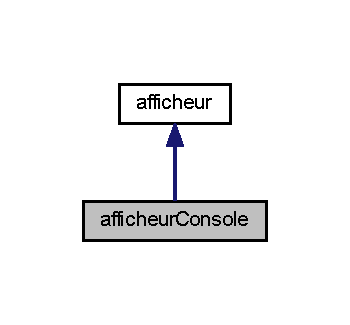
\includegraphics[width=168pt]{classafficheur_console__inherit__graph}
\end{center}
\end{figure}


Collaboration diagram for afficheur\+Console\+:\nopagebreak
\begin{figure}[H]
\begin{center}
\leavevmode
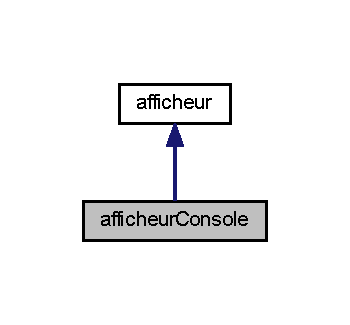
\includegraphics[width=168pt]{classafficheur_console__coll__graph}
\end{center}
\end{figure}
\subsection*{Public Member Functions}
\begin{DoxyCompactItemize}
\item 
\hyperlink{classafficheur_console_a5d5b09077e150ddb11f0dc5b9cf89f6f}{afficheur\+Console} ()=default
\item 
virtual \hyperlink{classafficheur_console_a0f902699d385726ea9d9889d37e57558}{$\sim$afficheur\+Console} ()
\begin{DoxyCompactList}\small\item\em Destructeur virtuel de l\textquotesingle{}objet \hyperlink{classafficheur_console}{afficheur\+Console}. \end{DoxyCompactList}\item 
virtual void \hyperlink{classafficheur_console_a0930128cabb9b2585db0140f7614a3df}{affiche\+Semaine} (const \hyperlink{classhoraire}{horaire} $\ast$h, ostream \&ost) override
\begin{DoxyCompactList}\small\item\em Renvoie dans ost le numero de la semaine de l\textquotesingle{}horaire h. \end{DoxyCompactList}\item 
virtual void \hyperlink{classafficheur_console_a842884a9553df737f781d2f8f040d30e}{affiche\+Heure} (const \hyperlink{classhoraire}{horaire} $\ast$h, ostream \&ost) override
\item 
virtual void \hyperlink{classafficheur_console_a9d69206c3cd6409d1437ee546e71cf25}{affiche\+Jour} (const \hyperlink{classhoraire}{horaire} $\ast$h, ostream \&ost) override
\item 
virtual void \hyperlink{classafficheur_console_a44e40b275c8b0b1a33cdc5bd46a31cf3}{affiche\+Horaire} (const \hyperlink{classhoraire}{horaire} $\ast$h, ostream \&ost) override
\item 
virtual void \hyperlink{classafficheur_console_aa178d74ab314df687800c612a3615ed6}{affiche\+Professeur} (const \hyperlink{classprofesseur}{professeur} $\ast$p, ostream \&ost) override
\item 
virtual void \hyperlink{classafficheur_console_aa77bdd8065edd5269f83679490e78dee}{affiche\+Cours} (const \hyperlink{classcours}{cours} $\ast$c, ostream \&ost) override
\end{DoxyCompactItemize}


\subsection{Detailed Description}


Definition at line 11 of file afficheur\+Console.\+h.



\subsection{Constructor \& Destructor Documentation}
\hypertarget{classafficheur_console_a5d5b09077e150ddb11f0dc5b9cf89f6f}{}\label{classafficheur_console_a5d5b09077e150ddb11f0dc5b9cf89f6f} 
\index{afficheur\+Console@{afficheur\+Console}!afficheur\+Console@{afficheur\+Console}}
\index{afficheur\+Console@{afficheur\+Console}!afficheur\+Console@{afficheur\+Console}}
\subsubsection{\texorpdfstring{afficheur\+Console()}{afficheurConsole()}}
{\footnotesize\ttfamily afficheur\+Console\+::afficheur\+Console (\begin{DoxyParamCaption}{ }\end{DoxyParamCaption})\hspace{0.3cm}{\ttfamily [default]}}

\hypertarget{classafficheur_console_a0f902699d385726ea9d9889d37e57558}{}\label{classafficheur_console_a0f902699d385726ea9d9889d37e57558} 
\index{afficheur\+Console@{afficheur\+Console}!````~afficheur\+Console@{$\sim$afficheur\+Console}}
\index{````~afficheur\+Console@{$\sim$afficheur\+Console}!afficheur\+Console@{afficheur\+Console}}
\subsubsection{\texorpdfstring{$\sim$afficheur\+Console()}{~afficheurConsole()}}
{\footnotesize\ttfamily afficheur\+Console\+::$\sim$afficheur\+Console (\begin{DoxyParamCaption}{ }\end{DoxyParamCaption})\hspace{0.3cm}{\ttfamily [virtual]}}



Destructeur virtuel de l\textquotesingle{}objet \hyperlink{classafficheur_console}{afficheur\+Console}. 



Definition at line 13 of file afficheur\+Console.\+cpp.



\subsection{Member Function Documentation}
\hypertarget{classafficheur_console_aa77bdd8065edd5269f83679490e78dee}{}\label{classafficheur_console_aa77bdd8065edd5269f83679490e78dee} 
\index{afficheur\+Console@{afficheur\+Console}!affiche\+Cours@{affiche\+Cours}}
\index{affiche\+Cours@{affiche\+Cours}!afficheur\+Console@{afficheur\+Console}}
\subsubsection{\texorpdfstring{affiche\+Cours()}{afficheCours()}}
{\footnotesize\ttfamily void afficheur\+Console\+::affiche\+Cours (\begin{DoxyParamCaption}\item[{const \hyperlink{classcours}{cours} $\ast$}]{c,  }\item[{ostream \&}]{ost }\end{DoxyParamCaption})\hspace{0.3cm}{\ttfamily [override]}, {\ttfamily [virtual]}}



Implements \hyperlink{classafficheur_a9d176576ad45c2a07a8a887b853b7edb}{afficheur}.



Definition at line 79 of file afficheur\+Console.\+cpp.

\hypertarget{classafficheur_console_a842884a9553df737f781d2f8f040d30e}{}\label{classafficheur_console_a842884a9553df737f781d2f8f040d30e} 
\index{afficheur\+Console@{afficheur\+Console}!affiche\+Heure@{affiche\+Heure}}
\index{affiche\+Heure@{affiche\+Heure}!afficheur\+Console@{afficheur\+Console}}
\subsubsection{\texorpdfstring{affiche\+Heure()}{afficheHeure()}}
{\footnotesize\ttfamily void afficheur\+Console\+::affiche\+Heure (\begin{DoxyParamCaption}\item[{const \hyperlink{classhoraire}{horaire} $\ast$}]{h,  }\item[{ostream \&}]{ost }\end{DoxyParamCaption})\hspace{0.3cm}{\ttfamily [override]}, {\ttfamily [virtual]}}



Implements \hyperlink{classafficheur_a3c3ace0f2f01e95a1cc86a0b6c497e34}{afficheur}.



Definition at line 27 of file afficheur\+Console.\+cpp.

Here is the call graph for this function\+:\nopagebreak
\begin{figure}[H]
\begin{center}
\leavevmode
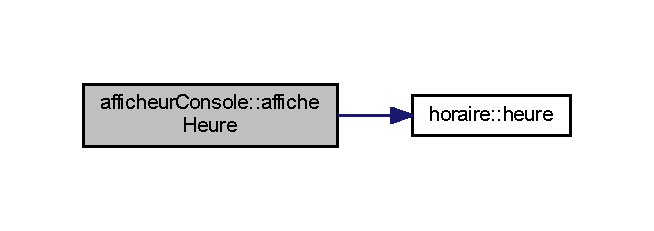
\includegraphics[width=314pt]{classafficheur_console_a842884a9553df737f781d2f8f040d30e_cgraph}
\end{center}
\end{figure}
Here is the caller graph for this function\+:\nopagebreak
\begin{figure}[H]
\begin{center}
\leavevmode
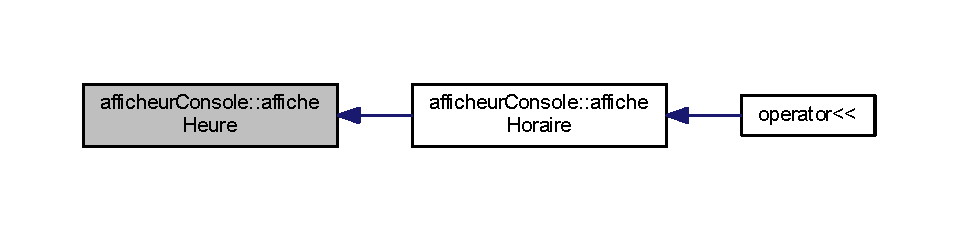
\includegraphics[width=350pt]{classafficheur_console_a842884a9553df737f781d2f8f040d30e_icgraph}
\end{center}
\end{figure}
\hypertarget{classafficheur_console_a44e40b275c8b0b1a33cdc5bd46a31cf3}{}\label{classafficheur_console_a44e40b275c8b0b1a33cdc5bd46a31cf3} 
\index{afficheur\+Console@{afficheur\+Console}!affiche\+Horaire@{affiche\+Horaire}}
\index{affiche\+Horaire@{affiche\+Horaire}!afficheur\+Console@{afficheur\+Console}}
\subsubsection{\texorpdfstring{affiche\+Horaire()}{afficheHoraire()}}
{\footnotesize\ttfamily void afficheur\+Console\+::affiche\+Horaire (\begin{DoxyParamCaption}\item[{const \hyperlink{classhoraire}{horaire} $\ast$}]{h,  }\item[{ostream \&}]{ost }\end{DoxyParamCaption})\hspace{0.3cm}{\ttfamily [override]}, {\ttfamily [virtual]}}



Implements \hyperlink{classafficheur_aa598626f11775b4c610b8f262017cad7}{afficheur}.



Definition at line 64 of file afficheur\+Console.\+cpp.

Here is the call graph for this function\+:\nopagebreak
\begin{figure}[H]
\begin{center}
\leavevmode
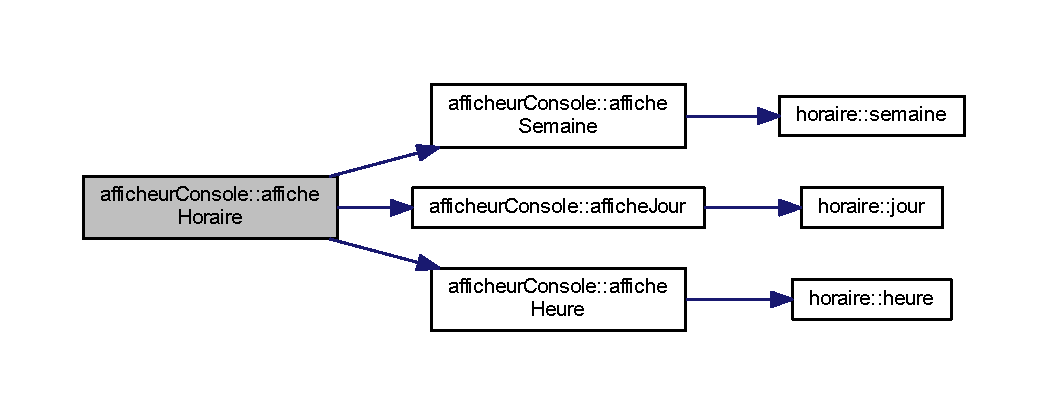
\includegraphics[width=350pt]{classafficheur_console_a44e40b275c8b0b1a33cdc5bd46a31cf3_cgraph}
\end{center}
\end{figure}
Here is the caller graph for this function\+:\nopagebreak
\begin{figure}[H]
\begin{center}
\leavevmode
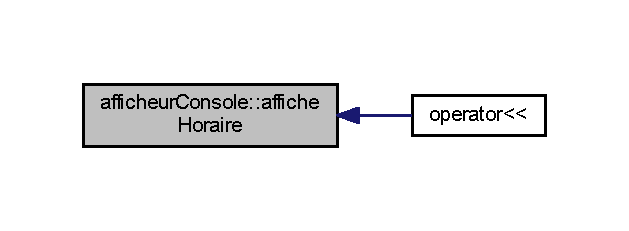
\includegraphics[width=302pt]{classafficheur_console_a44e40b275c8b0b1a33cdc5bd46a31cf3_icgraph}
\end{center}
\end{figure}
\hypertarget{classafficheur_console_a9d69206c3cd6409d1437ee546e71cf25}{}\label{classafficheur_console_a9d69206c3cd6409d1437ee546e71cf25} 
\index{afficheur\+Console@{afficheur\+Console}!affiche\+Jour@{affiche\+Jour}}
\index{affiche\+Jour@{affiche\+Jour}!afficheur\+Console@{afficheur\+Console}}
\subsubsection{\texorpdfstring{affiche\+Jour()}{afficheJour()}}
{\footnotesize\ttfamily void afficheur\+Console\+::affiche\+Jour (\begin{DoxyParamCaption}\item[{const \hyperlink{classhoraire}{horaire} $\ast$}]{h,  }\item[{ostream \&}]{ost }\end{DoxyParamCaption})\hspace{0.3cm}{\ttfamily [override]}, {\ttfamily [virtual]}}



Implements \hyperlink{classafficheur_a0cea335dad556ceba3487ae261b831f9}{afficheur}.



Definition at line 43 of file afficheur\+Console.\+cpp.

Here is the call graph for this function\+:\nopagebreak
\begin{figure}[H]
\begin{center}
\leavevmode
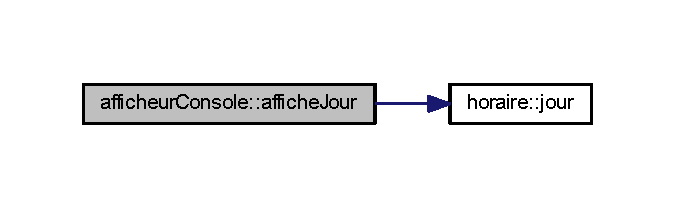
\includegraphics[width=324pt]{classafficheur_console_a9d69206c3cd6409d1437ee546e71cf25_cgraph}
\end{center}
\end{figure}
Here is the caller graph for this function\+:\nopagebreak
\begin{figure}[H]
\begin{center}
\leavevmode
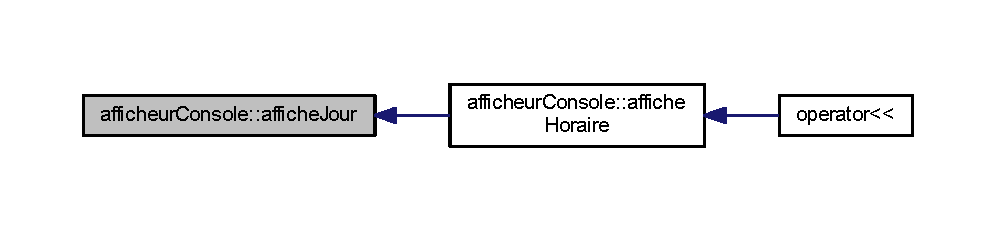
\includegraphics[width=350pt]{classafficheur_console_a9d69206c3cd6409d1437ee546e71cf25_icgraph}
\end{center}
\end{figure}
\hypertarget{classafficheur_console_aa178d74ab314df687800c612a3615ed6}{}\label{classafficheur_console_aa178d74ab314df687800c612a3615ed6} 
\index{afficheur\+Console@{afficheur\+Console}!affiche\+Professeur@{affiche\+Professeur}}
\index{affiche\+Professeur@{affiche\+Professeur}!afficheur\+Console@{afficheur\+Console}}
\subsubsection{\texorpdfstring{affiche\+Professeur()}{afficheProfesseur()}}
{\footnotesize\ttfamily void afficheur\+Console\+::affiche\+Professeur (\begin{DoxyParamCaption}\item[{const \hyperlink{classprofesseur}{professeur} $\ast$}]{p,  }\item[{ostream \&}]{ost }\end{DoxyParamCaption})\hspace{0.3cm}{\ttfamily [override]}, {\ttfamily [virtual]}}



Implements \hyperlink{classafficheur_a54b3e457d56738ed20641e5546872142}{afficheur}.



Definition at line 74 of file afficheur\+Console.\+cpp.

Here is the call graph for this function\+:\nopagebreak
\begin{figure}[H]
\begin{center}
\leavevmode
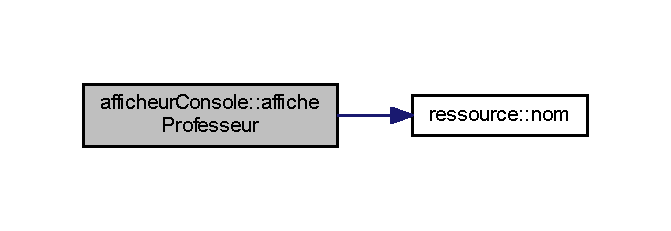
\includegraphics[width=322pt]{classafficheur_console_aa178d74ab314df687800c612a3615ed6_cgraph}
\end{center}
\end{figure}
Here is the caller graph for this function\+:\nopagebreak
\begin{figure}[H]
\begin{center}
\leavevmode
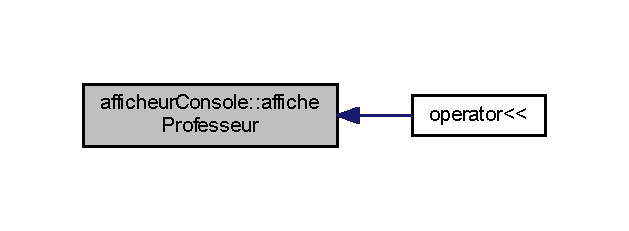
\includegraphics[width=302pt]{classafficheur_console_aa178d74ab314df687800c612a3615ed6_icgraph}
\end{center}
\end{figure}
\hypertarget{classafficheur_console_a0930128cabb9b2585db0140f7614a3df}{}\label{classafficheur_console_a0930128cabb9b2585db0140f7614a3df} 
\index{afficheur\+Console@{afficheur\+Console}!affiche\+Semaine@{affiche\+Semaine}}
\index{affiche\+Semaine@{affiche\+Semaine}!afficheur\+Console@{afficheur\+Console}}
\subsubsection{\texorpdfstring{affiche\+Semaine()}{afficheSemaine()}}
{\footnotesize\ttfamily void afficheur\+Console\+::affiche\+Semaine (\begin{DoxyParamCaption}\item[{const \hyperlink{classhoraire}{horaire} $\ast$}]{h,  }\item[{ostream \&}]{ost }\end{DoxyParamCaption})\hspace{0.3cm}{\ttfamily [override]}, {\ttfamily [virtual]}}



Renvoie dans ost le numero de la semaine de l\textquotesingle{}horaire h. 


\begin{DoxyParams}[1]{Parameters}
\mbox{\tt in}  & {\em h} & -\/ un objet de type horaire \\
\hline
\mbox{\tt out}  & {\em ost} & -\/ flux de sortie \\
\hline
\end{DoxyParams}


Implements \hyperlink{classafficheur_a1551534b5916a48d3ea73f0d68929e95}{afficheur}.



Definition at line 21 of file afficheur\+Console.\+cpp.

Here is the call graph for this function\+:\nopagebreak
\begin{figure}[H]
\begin{center}
\leavevmode
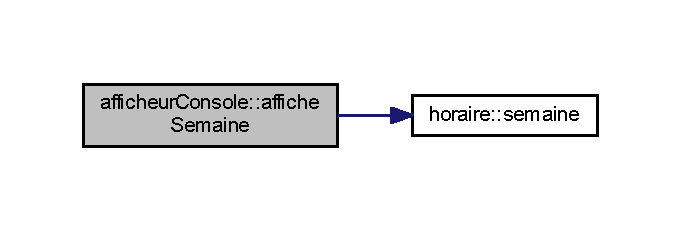
\includegraphics[width=327pt]{classafficheur_console_a0930128cabb9b2585db0140f7614a3df_cgraph}
\end{center}
\end{figure}
Here is the caller graph for this function\+:\nopagebreak
\begin{figure}[H]
\begin{center}
\leavevmode
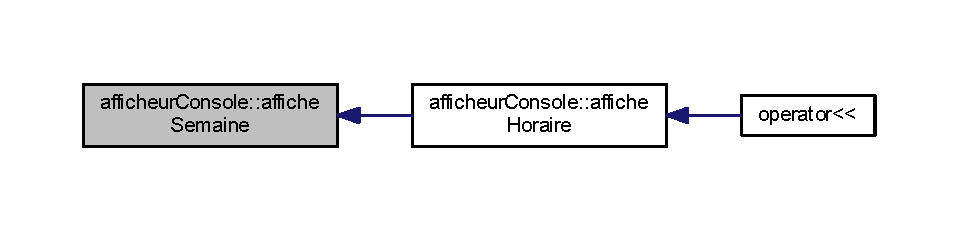
\includegraphics[width=350pt]{classafficheur_console_a0930128cabb9b2585db0140f7614a3df_icgraph}
\end{center}
\end{figure}


The documentation for this class was generated from the following files\+:\begin{DoxyCompactItemize}
\item 
lib/\hyperlink{afficheur_console_8h}{afficheur\+Console.\+h}\item 
cpp/\hyperlink{afficheur_console_8cpp}{afficheur\+Console.\+cpp}\end{DoxyCompactItemize}

\hypertarget{class_catch_1_1_matchers_1_1_impl_1_1_generic_1_1_all_of}{}\section{Catch\+:\+:Matchers\+:\+:Impl\+:\+:Generic\+:\+:All\+Of$<$ ExpressionT $>$ Class Template Reference}
\label{class_catch_1_1_matchers_1_1_impl_1_1_generic_1_1_all_of}\index{Catch\+::\+Matchers\+::\+Impl\+::\+Generic\+::\+All\+Of$<$ Expression\+T $>$@{Catch\+::\+Matchers\+::\+Impl\+::\+Generic\+::\+All\+Of$<$ Expression\+T $>$}}


{\ttfamily \#include $<$catch.\+hpp$>$}



Inheritance diagram for Catch\+:\+:Matchers\+:\+:Impl\+:\+:Generic\+:\+:All\+Of$<$ ExpressionT $>$\+:\nopagebreak
\begin{figure}[H]
\begin{center}
\leavevmode
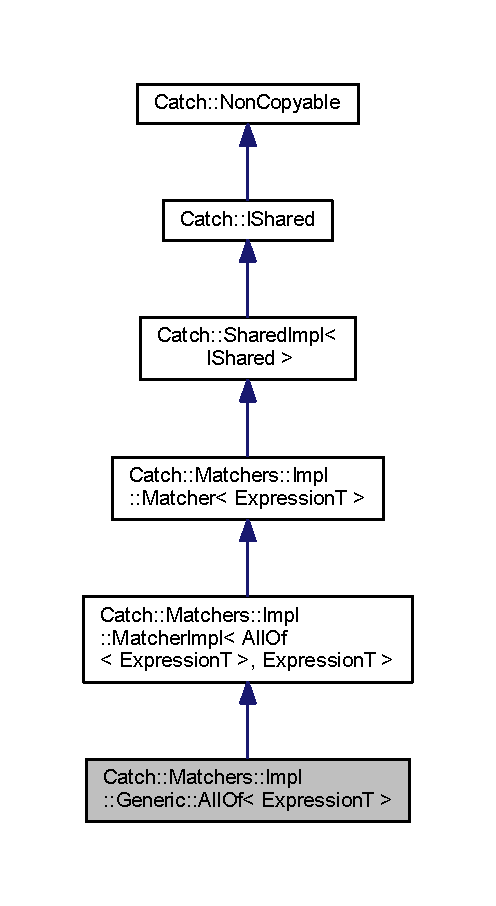
\includegraphics[width=238pt]{class_catch_1_1_matchers_1_1_impl_1_1_generic_1_1_all_of__inherit__graph}
\end{center}
\end{figure}


Collaboration diagram for Catch\+:\+:Matchers\+:\+:Impl\+:\+:Generic\+:\+:All\+Of$<$ ExpressionT $>$\+:\nopagebreak
\begin{figure}[H]
\begin{center}
\leavevmode
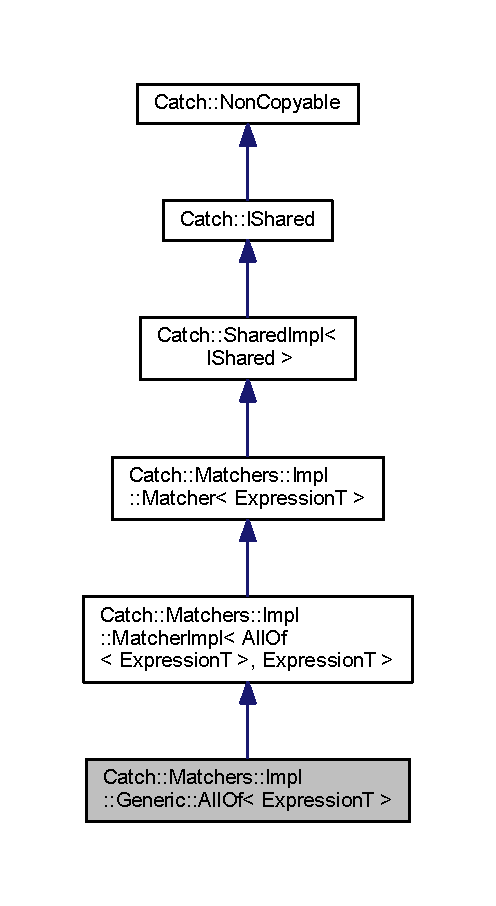
\includegraphics[width=238pt]{class_catch_1_1_matchers_1_1_impl_1_1_generic_1_1_all_of__coll__graph}
\end{center}
\end{figure}
\subsection*{Public Member Functions}
\begin{DoxyCompactItemize}
\item 
\hyperlink{class_catch_1_1_matchers_1_1_impl_1_1_generic_1_1_all_of_a9dfcc2f0549114f3b50cc65a2e10c996}{All\+Of} ()
\item 
\hyperlink{class_catch_1_1_matchers_1_1_impl_1_1_generic_1_1_all_of_a31f7c5e570e79bdf64064ee87c331a59}{All\+Of} (\hyperlink{class_catch_1_1_matchers_1_1_impl_1_1_generic_1_1_all_of}{All\+Of} const \&other)
\item 
\hyperlink{class_catch_1_1_matchers_1_1_impl_1_1_generic_1_1_all_of}{All\+Of} \& \hyperlink{class_catch_1_1_matchers_1_1_impl_1_1_generic_1_1_all_of_a8c5cd1e494ab697076da418ee72ac297}{add} (\hyperlink{struct_catch_1_1_matchers_1_1_impl_1_1_matcher}{Matcher}$<$ ExpressionT $>$ const \&matcher)
\item 
virtual bool \hyperlink{class_catch_1_1_matchers_1_1_impl_1_1_generic_1_1_all_of_a95231b6a455e1a646d0b54bce55138be}{match} (ExpressionT const \&expr) const
\item 
virtual std\+::string \hyperlink{class_catch_1_1_matchers_1_1_impl_1_1_generic_1_1_all_of_a8c8e7742501dc81e51a3c745d6f74119}{to\+String} () const
\item 
\hyperlink{class_catch_1_1_matchers_1_1_impl_1_1_generic_1_1_all_of}{All\+Of} \hyperlink{class_catch_1_1_matchers_1_1_impl_1_1_generic_1_1_all_of_aca6497aaa7fdb6560ebe850f32ccbf15}{operator\&\&} (\hyperlink{struct_catch_1_1_matchers_1_1_impl_1_1_matcher}{Matcher}$<$ ExpressionT $>$ const \&other) const
\end{DoxyCompactItemize}
\subsection*{Additional Inherited Members}


\subsection{Detailed Description}
\subsubsection*{template$<$typename ExpressionT$>$\newline
class Catch\+::\+Matchers\+::\+Impl\+::\+Generic\+::\+All\+Of$<$ Expression\+T $>$}



Definition at line 898 of file catch.\+hpp.



\subsection{Constructor \& Destructor Documentation}
\hypertarget{class_catch_1_1_matchers_1_1_impl_1_1_generic_1_1_all_of_a9dfcc2f0549114f3b50cc65a2e10c996}{}\label{class_catch_1_1_matchers_1_1_impl_1_1_generic_1_1_all_of_a9dfcc2f0549114f3b50cc65a2e10c996} 
\index{Catch\+::\+Matchers\+::\+Impl\+::\+Generic\+::\+All\+Of@{Catch\+::\+Matchers\+::\+Impl\+::\+Generic\+::\+All\+Of}!All\+Of@{All\+Of}}
\index{All\+Of@{All\+Of}!Catch\+::\+Matchers\+::\+Impl\+::\+Generic\+::\+All\+Of@{Catch\+::\+Matchers\+::\+Impl\+::\+Generic\+::\+All\+Of}}
\subsubsection{\texorpdfstring{All\+Of()}{AllOf()}\hspace{0.1cm}{\footnotesize\ttfamily [1/2]}}
{\footnotesize\ttfamily template$<$typename ExpressionT$>$ \\
\hyperlink{class_catch_1_1_matchers_1_1_impl_1_1_generic_1_1_all_of}{Catch\+::\+Matchers\+::\+Impl\+::\+Generic\+::\+All\+Of}$<$ ExpressionT $>$\+::\hyperlink{class_catch_1_1_matchers_1_1_impl_1_1_generic_1_1_all_of}{All\+Of} (\begin{DoxyParamCaption}{ }\end{DoxyParamCaption})\hspace{0.3cm}{\ttfamily [inline]}}



Definition at line 948 of file catch.\+hpp.

\hypertarget{class_catch_1_1_matchers_1_1_impl_1_1_generic_1_1_all_of_a31f7c5e570e79bdf64064ee87c331a59}{}\label{class_catch_1_1_matchers_1_1_impl_1_1_generic_1_1_all_of_a31f7c5e570e79bdf64064ee87c331a59} 
\index{Catch\+::\+Matchers\+::\+Impl\+::\+Generic\+::\+All\+Of@{Catch\+::\+Matchers\+::\+Impl\+::\+Generic\+::\+All\+Of}!All\+Of@{All\+Of}}
\index{All\+Of@{All\+Of}!Catch\+::\+Matchers\+::\+Impl\+::\+Generic\+::\+All\+Of@{Catch\+::\+Matchers\+::\+Impl\+::\+Generic\+::\+All\+Of}}
\subsubsection{\texorpdfstring{All\+Of()}{AllOf()}\hspace{0.1cm}{\footnotesize\ttfamily [2/2]}}
{\footnotesize\ttfamily template$<$typename ExpressionT$>$ \\
\hyperlink{class_catch_1_1_matchers_1_1_impl_1_1_generic_1_1_all_of}{Catch\+::\+Matchers\+::\+Impl\+::\+Generic\+::\+All\+Of}$<$ ExpressionT $>$\+::\hyperlink{class_catch_1_1_matchers_1_1_impl_1_1_generic_1_1_all_of}{All\+Of} (\begin{DoxyParamCaption}\item[{\hyperlink{class_catch_1_1_matchers_1_1_impl_1_1_generic_1_1_all_of}{All\+Of}$<$ ExpressionT $>$ const \&}]{other }\end{DoxyParamCaption})\hspace{0.3cm}{\ttfamily [inline]}}



Definition at line 949 of file catch.\+hpp.



\subsection{Member Function Documentation}
\hypertarget{class_catch_1_1_matchers_1_1_impl_1_1_generic_1_1_all_of_a8c5cd1e494ab697076da418ee72ac297}{}\label{class_catch_1_1_matchers_1_1_impl_1_1_generic_1_1_all_of_a8c5cd1e494ab697076da418ee72ac297} 
\index{Catch\+::\+Matchers\+::\+Impl\+::\+Generic\+::\+All\+Of@{Catch\+::\+Matchers\+::\+Impl\+::\+Generic\+::\+All\+Of}!add@{add}}
\index{add@{add}!Catch\+::\+Matchers\+::\+Impl\+::\+Generic\+::\+All\+Of@{Catch\+::\+Matchers\+::\+Impl\+::\+Generic\+::\+All\+Of}}
\subsubsection{\texorpdfstring{add()}{add()}}
{\footnotesize\ttfamily template$<$typename ExpressionT$>$ \\
\hyperlink{class_catch_1_1_matchers_1_1_impl_1_1_generic_1_1_all_of}{All\+Of}\& \hyperlink{class_catch_1_1_matchers_1_1_impl_1_1_generic_1_1_all_of}{Catch\+::\+Matchers\+::\+Impl\+::\+Generic\+::\+All\+Of}$<$ ExpressionT $>$\+::add (\begin{DoxyParamCaption}\item[{\hyperlink{struct_catch_1_1_matchers_1_1_impl_1_1_matcher}{Matcher}$<$ ExpressionT $>$ const \&}]{matcher }\end{DoxyParamCaption})\hspace{0.3cm}{\ttfamily [inline]}}



Definition at line 951 of file catch.\+hpp.

Here is the call graph for this function\+:\nopagebreak
\begin{figure}[H]
\begin{center}
\leavevmode
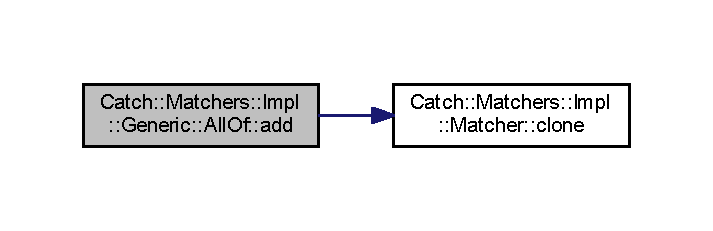
\includegraphics[width=342pt]{class_catch_1_1_matchers_1_1_impl_1_1_generic_1_1_all_of_a8c5cd1e494ab697076da418ee72ac297_cgraph}
\end{center}
\end{figure}
Here is the caller graph for this function\+:\nopagebreak
\begin{figure}[H]
\begin{center}
\leavevmode
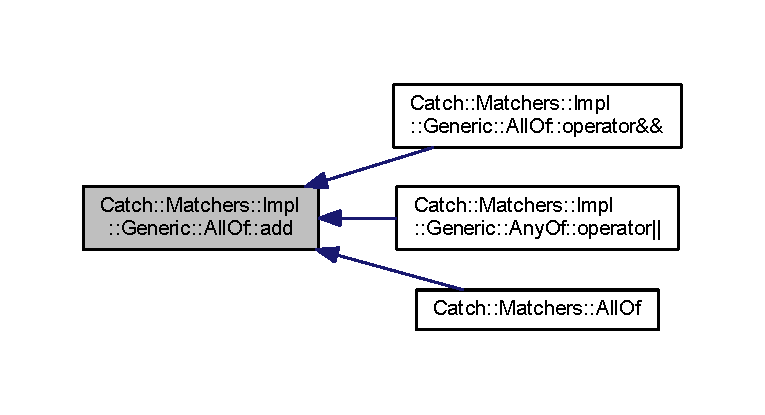
\includegraphics[width=350pt]{class_catch_1_1_matchers_1_1_impl_1_1_generic_1_1_all_of_a8c5cd1e494ab697076da418ee72ac297_icgraph}
\end{center}
\end{figure}
\hypertarget{class_catch_1_1_matchers_1_1_impl_1_1_generic_1_1_all_of_a95231b6a455e1a646d0b54bce55138be}{}\label{class_catch_1_1_matchers_1_1_impl_1_1_generic_1_1_all_of_a95231b6a455e1a646d0b54bce55138be} 
\index{Catch\+::\+Matchers\+::\+Impl\+::\+Generic\+::\+All\+Of@{Catch\+::\+Matchers\+::\+Impl\+::\+Generic\+::\+All\+Of}!match@{match}}
\index{match@{match}!Catch\+::\+Matchers\+::\+Impl\+::\+Generic\+::\+All\+Of@{Catch\+::\+Matchers\+::\+Impl\+::\+Generic\+::\+All\+Of}}
\subsubsection{\texorpdfstring{match()}{match()}}
{\footnotesize\ttfamily template$<$typename ExpressionT$>$ \\
virtual bool \hyperlink{class_catch_1_1_matchers_1_1_impl_1_1_generic_1_1_all_of}{Catch\+::\+Matchers\+::\+Impl\+::\+Generic\+::\+All\+Of}$<$ ExpressionT $>$\+::match (\begin{DoxyParamCaption}\item[{ExpressionT const \&}]{expr }\end{DoxyParamCaption}) const\hspace{0.3cm}{\ttfamily [inline]}, {\ttfamily [virtual]}}



Implements \hyperlink{struct_catch_1_1_matchers_1_1_impl_1_1_matcher_a8c1c5511ce1f3738a45e6901b558f583}{Catch\+::\+Matchers\+::\+Impl\+::\+Matcher$<$ Expression\+T $>$}.



Definition at line 955 of file catch.\+hpp.

\hypertarget{class_catch_1_1_matchers_1_1_impl_1_1_generic_1_1_all_of_aca6497aaa7fdb6560ebe850f32ccbf15}{}\label{class_catch_1_1_matchers_1_1_impl_1_1_generic_1_1_all_of_aca6497aaa7fdb6560ebe850f32ccbf15} 
\index{Catch\+::\+Matchers\+::\+Impl\+::\+Generic\+::\+All\+Of@{Catch\+::\+Matchers\+::\+Impl\+::\+Generic\+::\+All\+Of}!operator\&\&@{operator\&\&}}
\index{operator\&\&@{operator\&\&}!Catch\+::\+Matchers\+::\+Impl\+::\+Generic\+::\+All\+Of@{Catch\+::\+Matchers\+::\+Impl\+::\+Generic\+::\+All\+Of}}
\subsubsection{\texorpdfstring{operator\&\&()}{operator\&\&()}}
{\footnotesize\ttfamily template$<$typename ExpressionT$>$ \\
\hyperlink{class_catch_1_1_matchers_1_1_impl_1_1_generic_1_1_all_of}{All\+Of} \hyperlink{class_catch_1_1_matchers_1_1_impl_1_1_generic_1_1_all_of}{Catch\+::\+Matchers\+::\+Impl\+::\+Generic\+::\+All\+Of}$<$ ExpressionT $>$\+::operator \&\& (\begin{DoxyParamCaption}\item[{\hyperlink{struct_catch_1_1_matchers_1_1_impl_1_1_matcher}{Matcher}$<$ ExpressionT $>$ const \&}]{other }\end{DoxyParamCaption}) const\hspace{0.3cm}{\ttfamily [inline]}}



Definition at line 974 of file catch.\+hpp.

Here is the call graph for this function\+:\nopagebreak
\begin{figure}[H]
\begin{center}
\leavevmode
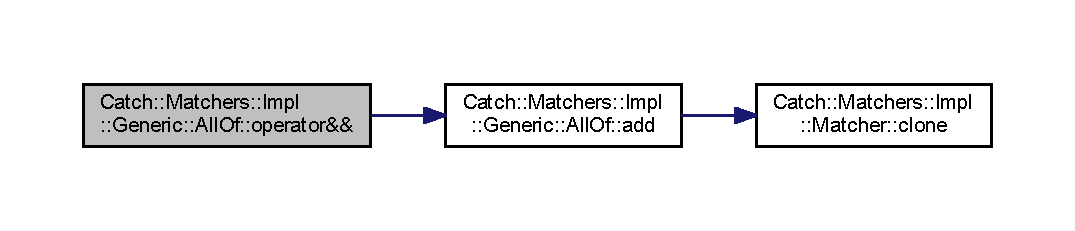
\includegraphics[width=350pt]{class_catch_1_1_matchers_1_1_impl_1_1_generic_1_1_all_of_aca6497aaa7fdb6560ebe850f32ccbf15_cgraph}
\end{center}
\end{figure}
\hypertarget{class_catch_1_1_matchers_1_1_impl_1_1_generic_1_1_all_of_a8c8e7742501dc81e51a3c745d6f74119}{}\label{class_catch_1_1_matchers_1_1_impl_1_1_generic_1_1_all_of_a8c8e7742501dc81e51a3c745d6f74119} 
\index{Catch\+::\+Matchers\+::\+Impl\+::\+Generic\+::\+All\+Of@{Catch\+::\+Matchers\+::\+Impl\+::\+Generic\+::\+All\+Of}!to\+String@{to\+String}}
\index{to\+String@{to\+String}!Catch\+::\+Matchers\+::\+Impl\+::\+Generic\+::\+All\+Of@{Catch\+::\+Matchers\+::\+Impl\+::\+Generic\+::\+All\+Of}}
\subsubsection{\texorpdfstring{to\+String()}{toString()}}
{\footnotesize\ttfamily template$<$typename ExpressionT$>$ \\
virtual std\+::string \hyperlink{class_catch_1_1_matchers_1_1_impl_1_1_generic_1_1_all_of}{Catch\+::\+Matchers\+::\+Impl\+::\+Generic\+::\+All\+Of}$<$ ExpressionT $>$\+::to\+String (\begin{DoxyParamCaption}{ }\end{DoxyParamCaption}) const\hspace{0.3cm}{\ttfamily [inline]}, {\ttfamily [virtual]}}



Implements \hyperlink{struct_catch_1_1_matchers_1_1_impl_1_1_matcher_a091bcc37e589967d7e10fc7790d820e2}{Catch\+::\+Matchers\+::\+Impl\+::\+Matcher$<$ Expression\+T $>$}.



Definition at line 962 of file catch.\+hpp.



The documentation for this class was generated from the following file\+:\begin{DoxyCompactItemize}
\item 
lib/\hyperlink{catch_8hpp}{catch.\+hpp}\end{DoxyCompactItemize}

\hypertarget{class_catch_1_1_matchers_1_1_impl_1_1_generic_1_1_any_of}{}\section{Catch\+:\+:Matchers\+:\+:Impl\+:\+:Generic\+:\+:Any\+Of$<$ ExpressionT $>$ Class Template Reference}
\label{class_catch_1_1_matchers_1_1_impl_1_1_generic_1_1_any_of}\index{Catch\+::\+Matchers\+::\+Impl\+::\+Generic\+::\+Any\+Of$<$ Expression\+T $>$@{Catch\+::\+Matchers\+::\+Impl\+::\+Generic\+::\+Any\+Of$<$ Expression\+T $>$}}


{\ttfamily \#include $<$catch.\+hpp$>$}



Inheritance diagram for Catch\+:\+:Matchers\+:\+:Impl\+:\+:Generic\+:\+:Any\+Of$<$ ExpressionT $>$\+:\nopagebreak
\begin{figure}[H]
\begin{center}
\leavevmode
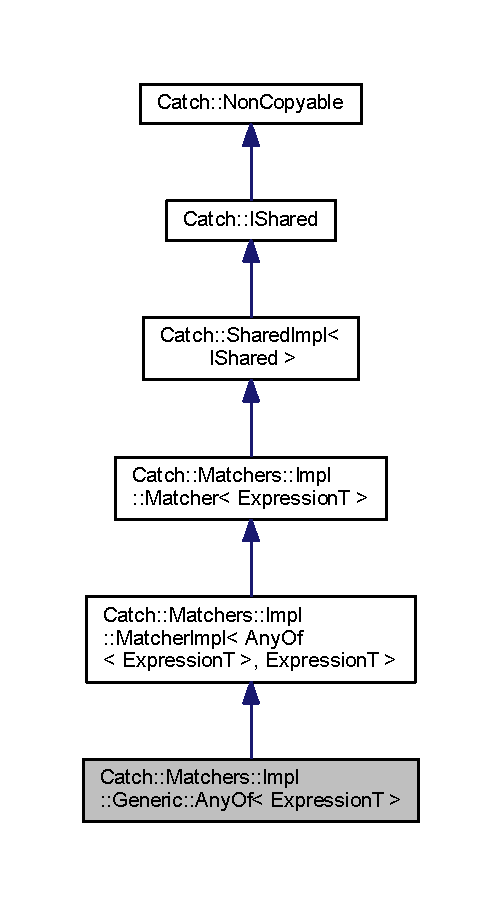
\includegraphics[width=241pt]{class_catch_1_1_matchers_1_1_impl_1_1_generic_1_1_any_of__inherit__graph}
\end{center}
\end{figure}


Collaboration diagram for Catch\+:\+:Matchers\+:\+:Impl\+:\+:Generic\+:\+:Any\+Of$<$ ExpressionT $>$\+:\nopagebreak
\begin{figure}[H]
\begin{center}
\leavevmode
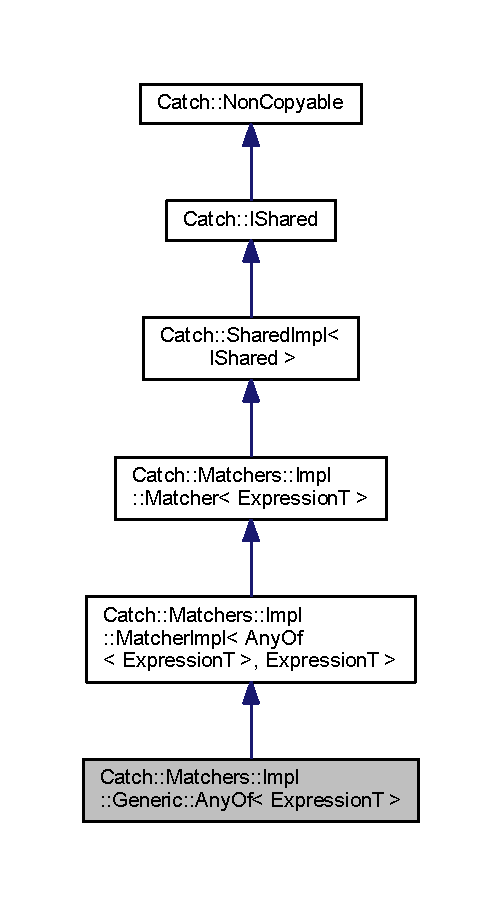
\includegraphics[width=241pt]{class_catch_1_1_matchers_1_1_impl_1_1_generic_1_1_any_of__coll__graph}
\end{center}
\end{figure}
\subsection*{Public Member Functions}
\begin{DoxyCompactItemize}
\item 
\hyperlink{class_catch_1_1_matchers_1_1_impl_1_1_generic_1_1_any_of_a131d84740c6b250ff7ef2213ae0de2aa}{Any\+Of} ()
\item 
\hyperlink{class_catch_1_1_matchers_1_1_impl_1_1_generic_1_1_any_of_a74fbc05b32d334fcbfd0fae0163a404e}{Any\+Of} (\hyperlink{class_catch_1_1_matchers_1_1_impl_1_1_generic_1_1_any_of}{Any\+Of} const \&other)
\item 
\hyperlink{class_catch_1_1_matchers_1_1_impl_1_1_generic_1_1_any_of}{Any\+Of} \& \hyperlink{class_catch_1_1_matchers_1_1_impl_1_1_generic_1_1_any_of_a3bce94b627551e5f96c5f9c6060413f0}{add} (\hyperlink{struct_catch_1_1_matchers_1_1_impl_1_1_matcher}{Matcher}$<$ ExpressionT $>$ const \&matcher)
\item 
virtual bool \hyperlink{class_catch_1_1_matchers_1_1_impl_1_1_generic_1_1_any_of_adebd5437cdb8e0d54e16e97fe26e7e85}{match} (ExpressionT const \&expr) const
\item 
virtual std\+::string \hyperlink{class_catch_1_1_matchers_1_1_impl_1_1_generic_1_1_any_of_a331aaf012b133682eadc9ed5342f848a}{to\+String} () const
\item 
\hyperlink{class_catch_1_1_matchers_1_1_impl_1_1_generic_1_1_any_of}{Any\+Of} \hyperlink{class_catch_1_1_matchers_1_1_impl_1_1_generic_1_1_any_of_a6dc9aee9a816f66ddc9de0c45c1c9ac1}{operator$\vert$$\vert$} (\hyperlink{struct_catch_1_1_matchers_1_1_impl_1_1_matcher}{Matcher}$<$ ExpressionT $>$ const \&other) const
\end{DoxyCompactItemize}
\subsection*{Additional Inherited Members}


\subsection{Constructor \& Destructor Documentation}
\hypertarget{class_catch_1_1_matchers_1_1_impl_1_1_generic_1_1_any_of_a131d84740c6b250ff7ef2213ae0de2aa}{}\label{class_catch_1_1_matchers_1_1_impl_1_1_generic_1_1_any_of_a131d84740c6b250ff7ef2213ae0de2aa} 
\index{Catch\+::\+Matchers\+::\+Impl\+::\+Generic\+::\+Any\+Of@{Catch\+::\+Matchers\+::\+Impl\+::\+Generic\+::\+Any\+Of}!Any\+Of@{Any\+Of}}
\index{Any\+Of@{Any\+Of}!Catch\+::\+Matchers\+::\+Impl\+::\+Generic\+::\+Any\+Of@{Catch\+::\+Matchers\+::\+Impl\+::\+Generic\+::\+Any\+Of}}
\subsubsection{\texorpdfstring{Any\+Of()}{AnyOf()}\hspace{0.1cm}{\footnotesize\ttfamily [1/2]}}
{\footnotesize\ttfamily template$<$typename ExpressionT$>$ \\
\hyperlink{class_catch_1_1_matchers_1_1_impl_1_1_generic_1_1_any_of}{Catch\+::\+Matchers\+::\+Impl\+::\+Generic\+::\+Any\+Of}$<$ ExpressionT $>$\+::\hyperlink{class_catch_1_1_matchers_1_1_impl_1_1_generic_1_1_any_of}{Any\+Of} (\begin{DoxyParamCaption}{ }\end{DoxyParamCaption})\hspace{0.3cm}{\ttfamily [inline]}}

\hypertarget{class_catch_1_1_matchers_1_1_impl_1_1_generic_1_1_any_of_a74fbc05b32d334fcbfd0fae0163a404e}{}\label{class_catch_1_1_matchers_1_1_impl_1_1_generic_1_1_any_of_a74fbc05b32d334fcbfd0fae0163a404e} 
\index{Catch\+::\+Matchers\+::\+Impl\+::\+Generic\+::\+Any\+Of@{Catch\+::\+Matchers\+::\+Impl\+::\+Generic\+::\+Any\+Of}!Any\+Of@{Any\+Of}}
\index{Any\+Of@{Any\+Of}!Catch\+::\+Matchers\+::\+Impl\+::\+Generic\+::\+Any\+Of@{Catch\+::\+Matchers\+::\+Impl\+::\+Generic\+::\+Any\+Of}}
\subsubsection{\texorpdfstring{Any\+Of()}{AnyOf()}\hspace{0.1cm}{\footnotesize\ttfamily [2/2]}}
{\footnotesize\ttfamily template$<$typename ExpressionT$>$ \\
\hyperlink{class_catch_1_1_matchers_1_1_impl_1_1_generic_1_1_any_of}{Catch\+::\+Matchers\+::\+Impl\+::\+Generic\+::\+Any\+Of}$<$ ExpressionT $>$\+::\hyperlink{class_catch_1_1_matchers_1_1_impl_1_1_generic_1_1_any_of}{Any\+Of} (\begin{DoxyParamCaption}\item[{\hyperlink{class_catch_1_1_matchers_1_1_impl_1_1_generic_1_1_any_of}{Any\+Of}$<$ ExpressionT $>$ const \&}]{other }\end{DoxyParamCaption})\hspace{0.3cm}{\ttfamily [inline]}}



\subsection{Member Function Documentation}
\hypertarget{class_catch_1_1_matchers_1_1_impl_1_1_generic_1_1_any_of_a3bce94b627551e5f96c5f9c6060413f0}{}\label{class_catch_1_1_matchers_1_1_impl_1_1_generic_1_1_any_of_a3bce94b627551e5f96c5f9c6060413f0} 
\index{Catch\+::\+Matchers\+::\+Impl\+::\+Generic\+::\+Any\+Of@{Catch\+::\+Matchers\+::\+Impl\+::\+Generic\+::\+Any\+Of}!add@{add}}
\index{add@{add}!Catch\+::\+Matchers\+::\+Impl\+::\+Generic\+::\+Any\+Of@{Catch\+::\+Matchers\+::\+Impl\+::\+Generic\+::\+Any\+Of}}
\subsubsection{\texorpdfstring{add()}{add()}}
{\footnotesize\ttfamily template$<$typename ExpressionT$>$ \\
\hyperlink{class_catch_1_1_matchers_1_1_impl_1_1_generic_1_1_any_of}{Any\+Of}\& \hyperlink{class_catch_1_1_matchers_1_1_impl_1_1_generic_1_1_any_of}{Catch\+::\+Matchers\+::\+Impl\+::\+Generic\+::\+Any\+Of}$<$ ExpressionT $>$\+::add (\begin{DoxyParamCaption}\item[{\hyperlink{struct_catch_1_1_matchers_1_1_impl_1_1_matcher}{Matcher}$<$ ExpressionT $>$ const \&}]{matcher }\end{DoxyParamCaption})\hspace{0.3cm}{\ttfamily [inline]}}

Here is the call graph for this function\+:\nopagebreak
\begin{figure}[H]
\begin{center}
\leavevmode
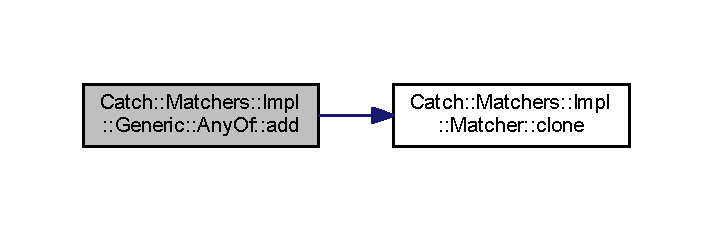
\includegraphics[width=342pt]{class_catch_1_1_matchers_1_1_impl_1_1_generic_1_1_any_of_a3bce94b627551e5f96c5f9c6060413f0_cgraph}
\end{center}
\end{figure}
Here is the caller graph for this function\+:\nopagebreak
\begin{figure}[H]
\begin{center}
\leavevmode
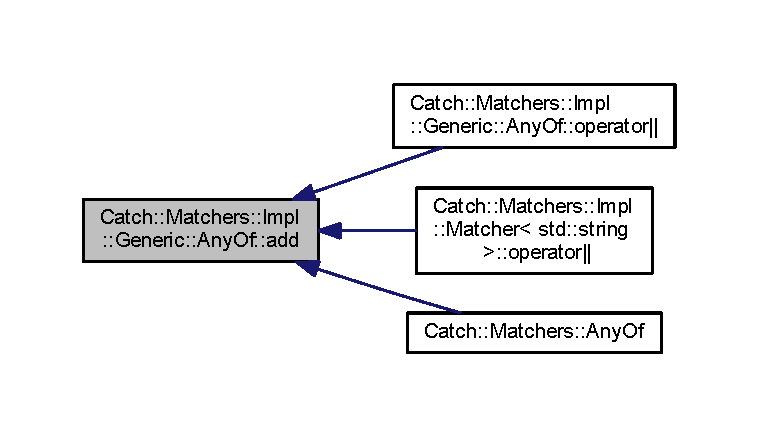
\includegraphics[width=350pt]{class_catch_1_1_matchers_1_1_impl_1_1_generic_1_1_any_of_a3bce94b627551e5f96c5f9c6060413f0_icgraph}
\end{center}
\end{figure}
\hypertarget{class_catch_1_1_matchers_1_1_impl_1_1_generic_1_1_any_of_adebd5437cdb8e0d54e16e97fe26e7e85}{}\label{class_catch_1_1_matchers_1_1_impl_1_1_generic_1_1_any_of_adebd5437cdb8e0d54e16e97fe26e7e85} 
\index{Catch\+::\+Matchers\+::\+Impl\+::\+Generic\+::\+Any\+Of@{Catch\+::\+Matchers\+::\+Impl\+::\+Generic\+::\+Any\+Of}!match@{match}}
\index{match@{match}!Catch\+::\+Matchers\+::\+Impl\+::\+Generic\+::\+Any\+Of@{Catch\+::\+Matchers\+::\+Impl\+::\+Generic\+::\+Any\+Of}}
\subsubsection{\texorpdfstring{match()}{match()}}
{\footnotesize\ttfamily template$<$typename ExpressionT$>$ \\
virtual bool \hyperlink{class_catch_1_1_matchers_1_1_impl_1_1_generic_1_1_any_of}{Catch\+::\+Matchers\+::\+Impl\+::\+Generic\+::\+Any\+Of}$<$ ExpressionT $>$\+::match (\begin{DoxyParamCaption}\item[{ExpressionT const \&}]{expr }\end{DoxyParamCaption}) const\hspace{0.3cm}{\ttfamily [inline]}, {\ttfamily [virtual]}}



Implements \hyperlink{struct_catch_1_1_matchers_1_1_impl_1_1_matcher_a8c1c5511ce1f3738a45e6901b558f583}{Catch\+::\+Matchers\+::\+Impl\+::\+Matcher$<$ Expression\+T $>$}.

\hypertarget{class_catch_1_1_matchers_1_1_impl_1_1_generic_1_1_any_of_a6dc9aee9a816f66ddc9de0c45c1c9ac1}{}\label{class_catch_1_1_matchers_1_1_impl_1_1_generic_1_1_any_of_a6dc9aee9a816f66ddc9de0c45c1c9ac1} 
\index{Catch\+::\+Matchers\+::\+Impl\+::\+Generic\+::\+Any\+Of@{Catch\+::\+Matchers\+::\+Impl\+::\+Generic\+::\+Any\+Of}!operator\texttt{"|}\texttt{"|}@{operator\texttt{"|}\texttt{"|}}}
\index{operator\texttt{"|}\texttt{"|}@{operator\texttt{"|}\texttt{"|}}!Catch\+::\+Matchers\+::\+Impl\+::\+Generic\+::\+Any\+Of@{Catch\+::\+Matchers\+::\+Impl\+::\+Generic\+::\+Any\+Of}}
\subsubsection{\texorpdfstring{operator\texttt{"|}\texttt{"|}()}{operator||()}}
{\footnotesize\ttfamily template$<$typename ExpressionT$>$ \\
\hyperlink{class_catch_1_1_matchers_1_1_impl_1_1_generic_1_1_any_of}{Any\+Of} \hyperlink{class_catch_1_1_matchers_1_1_impl_1_1_generic_1_1_any_of}{Catch\+::\+Matchers\+::\+Impl\+::\+Generic\+::\+Any\+Of}$<$ ExpressionT $>$\+::operator$\vert$$\vert$ (\begin{DoxyParamCaption}\item[{\hyperlink{struct_catch_1_1_matchers_1_1_impl_1_1_matcher}{Matcher}$<$ ExpressionT $>$ const \&}]{other }\end{DoxyParamCaption}) const\hspace{0.3cm}{\ttfamily [inline]}}

Here is the call graph for this function\+:\nopagebreak
\begin{figure}[H]
\begin{center}
\leavevmode
\includegraphics[width=350pt]{class_catch_1_1_matchers_1_1_impl_1_1_generic_1_1_any_of_a6dc9aee9a816f66ddc9de0c45c1c9ac1_cgraph}
\end{center}
\end{figure}
\hypertarget{class_catch_1_1_matchers_1_1_impl_1_1_generic_1_1_any_of_a331aaf012b133682eadc9ed5342f848a}{}\label{class_catch_1_1_matchers_1_1_impl_1_1_generic_1_1_any_of_a331aaf012b133682eadc9ed5342f848a} 
\index{Catch\+::\+Matchers\+::\+Impl\+::\+Generic\+::\+Any\+Of@{Catch\+::\+Matchers\+::\+Impl\+::\+Generic\+::\+Any\+Of}!to\+String@{to\+String}}
\index{to\+String@{to\+String}!Catch\+::\+Matchers\+::\+Impl\+::\+Generic\+::\+Any\+Of@{Catch\+::\+Matchers\+::\+Impl\+::\+Generic\+::\+Any\+Of}}
\subsubsection{\texorpdfstring{to\+String()}{toString()}}
{\footnotesize\ttfamily template$<$typename ExpressionT$>$ \\
virtual std\+::string \hyperlink{class_catch_1_1_matchers_1_1_impl_1_1_generic_1_1_any_of}{Catch\+::\+Matchers\+::\+Impl\+::\+Generic\+::\+Any\+Of}$<$ ExpressionT $>$\+::to\+String (\begin{DoxyParamCaption}{ }\end{DoxyParamCaption}) const\hspace{0.3cm}{\ttfamily [inline]}, {\ttfamily [virtual]}}



Implements \hyperlink{struct_catch_1_1_matchers_1_1_impl_1_1_matcher_a091bcc37e589967d7e10fc7790d820e2}{Catch\+::\+Matchers\+::\+Impl\+::\+Matcher$<$ Expression\+T $>$}.



The documentation for this class was generated from the following file\+:\begin{DoxyCompactItemize}
\item 
lib/\hyperlink{catch_8hpp}{catch.\+hpp}\end{DoxyCompactItemize}

\hypertarget{class_catch_1_1_detail_1_1_approx}{}\section{Catch\+:\+:Detail\+:\+:Approx Class Reference}
\label{class_catch_1_1_detail_1_1_approx}\index{Catch\+::\+Detail\+::\+Approx@{Catch\+::\+Detail\+::\+Approx}}


{\ttfamily \#include $<$catch.\+hpp$>$}

\subsection*{Public Member Functions}
\begin{DoxyCompactItemize}
\item 
\hyperlink{class_catch_1_1_detail_1_1_approx_a1a8618ea8db08c66bd3d9fe8f74b957a}{Approx} (double value)
\item 
\hyperlink{class_catch_1_1_detail_1_1_approx_a807330c63266fc914abdf6e461255a54}{Approx} (\hyperlink{class_catch_1_1_detail_1_1_approx}{Approx} const \&other)
\item 
\hyperlink{class_catch_1_1_detail_1_1_approx}{Approx} \hyperlink{class_catch_1_1_detail_1_1_approx_a48c9cbc28a05dc9dc8c3973b9eae2268}{operator()} (double value)
\item 
\hyperlink{class_catch_1_1_detail_1_1_approx}{Approx} \& \hyperlink{class_catch_1_1_detail_1_1_approx_a05c50c3ad0a971fab19345b5d94979a9}{epsilon} (double new\+Epsilon)
\item 
\hyperlink{class_catch_1_1_detail_1_1_approx}{Approx} \& \hyperlink{class_catch_1_1_detail_1_1_approx_acd80f0737bf38112beacd5ca95bef113}{scale} (double new\+Scale)
\item 
std\+::string \hyperlink{class_catch_1_1_detail_1_1_approx_a972fd9ac60607483263f1b0f0f9955e6}{to\+String} () const
\end{DoxyCompactItemize}
\subsection*{Static Public Member Functions}
\begin{DoxyCompactItemize}
\item 
static \hyperlink{class_catch_1_1_detail_1_1_approx}{Approx} \hyperlink{class_catch_1_1_detail_1_1_approx_aaf86dc0ee92272ac2d9839197a07951d}{custom} ()
\end{DoxyCompactItemize}
\subsection*{Friends}
\begin{DoxyCompactItemize}
\item 
bool \hyperlink{class_catch_1_1_detail_1_1_approx_ac766f044f1c63f0c5997982baefd9049}{operator==} (double lhs, \hyperlink{class_catch_1_1_detail_1_1_approx}{Approx} const \&rhs)
\item 
bool \hyperlink{class_catch_1_1_detail_1_1_approx_a35999631e6cef569f9da9f3fa910db22}{operator==} (\hyperlink{class_catch_1_1_detail_1_1_approx}{Approx} const \&lhs, double rhs)
\item 
bool \hyperlink{class_catch_1_1_detail_1_1_approx_a83b3763569a7ecc143c335b630be0e47}{operator!=} (double lhs, \hyperlink{class_catch_1_1_detail_1_1_approx}{Approx} const \&rhs)
\item 
bool \hyperlink{class_catch_1_1_detail_1_1_approx_a7497ef839f8026cc0edd6269a80f3e09}{operator!=} (\hyperlink{class_catch_1_1_detail_1_1_approx}{Approx} const \&lhs, double rhs)
\end{DoxyCompactItemize}


\subsection{Constructor \& Destructor Documentation}
\hypertarget{class_catch_1_1_detail_1_1_approx_a1a8618ea8db08c66bd3d9fe8f74b957a}{}\label{class_catch_1_1_detail_1_1_approx_a1a8618ea8db08c66bd3d9fe8f74b957a} 
\index{Catch\+::\+Detail\+::\+Approx@{Catch\+::\+Detail\+::\+Approx}!Approx@{Approx}}
\index{Approx@{Approx}!Catch\+::\+Detail\+::\+Approx@{Catch\+::\+Detail\+::\+Approx}}
\subsubsection{\texorpdfstring{Approx()}{Approx()}\hspace{0.1cm}{\footnotesize\ttfamily [1/2]}}
{\footnotesize\ttfamily Catch\+::\+Detail\+::\+Approx\+::\+Approx (\begin{DoxyParamCaption}\item[{double}]{value }\end{DoxyParamCaption})\hspace{0.3cm}{\ttfamily [inline]}, {\ttfamily [explicit]}}

\hypertarget{class_catch_1_1_detail_1_1_approx_a807330c63266fc914abdf6e461255a54}{}\label{class_catch_1_1_detail_1_1_approx_a807330c63266fc914abdf6e461255a54} 
\index{Catch\+::\+Detail\+::\+Approx@{Catch\+::\+Detail\+::\+Approx}!Approx@{Approx}}
\index{Approx@{Approx}!Catch\+::\+Detail\+::\+Approx@{Catch\+::\+Detail\+::\+Approx}}
\subsubsection{\texorpdfstring{Approx()}{Approx()}\hspace{0.1cm}{\footnotesize\ttfamily [2/2]}}
{\footnotesize\ttfamily Catch\+::\+Detail\+::\+Approx\+::\+Approx (\begin{DoxyParamCaption}\item[{\hyperlink{class_catch_1_1_detail_1_1_approx}{Approx} const \&}]{other }\end{DoxyParamCaption})\hspace{0.3cm}{\ttfamily [inline]}}



\subsection{Member Function Documentation}
\hypertarget{class_catch_1_1_detail_1_1_approx_aaf86dc0ee92272ac2d9839197a07951d}{}\label{class_catch_1_1_detail_1_1_approx_aaf86dc0ee92272ac2d9839197a07951d} 
\index{Catch\+::\+Detail\+::\+Approx@{Catch\+::\+Detail\+::\+Approx}!custom@{custom}}
\index{custom@{custom}!Catch\+::\+Detail\+::\+Approx@{Catch\+::\+Detail\+::\+Approx}}
\subsubsection{\texorpdfstring{custom()}{custom()}}
{\footnotesize\ttfamily static \hyperlink{class_catch_1_1_detail_1_1_approx}{Approx} Catch\+::\+Detail\+::\+Approx\+::custom (\begin{DoxyParamCaption}{ }\end{DoxyParamCaption})\hspace{0.3cm}{\ttfamily [inline]}, {\ttfamily [static]}}

\hypertarget{class_catch_1_1_detail_1_1_approx_a05c50c3ad0a971fab19345b5d94979a9}{}\label{class_catch_1_1_detail_1_1_approx_a05c50c3ad0a971fab19345b5d94979a9} 
\index{Catch\+::\+Detail\+::\+Approx@{Catch\+::\+Detail\+::\+Approx}!epsilon@{epsilon}}
\index{epsilon@{epsilon}!Catch\+::\+Detail\+::\+Approx@{Catch\+::\+Detail\+::\+Approx}}
\subsubsection{\texorpdfstring{epsilon()}{epsilon()}}
{\footnotesize\ttfamily \hyperlink{class_catch_1_1_detail_1_1_approx}{Approx}\& Catch\+::\+Detail\+::\+Approx\+::epsilon (\begin{DoxyParamCaption}\item[{double}]{new\+Epsilon }\end{DoxyParamCaption})\hspace{0.3cm}{\ttfamily [inline]}}

Here is the caller graph for this function\+:\nopagebreak
\begin{figure}[H]
\begin{center}
\leavevmode
\includegraphics[width=336pt]{class_catch_1_1_detail_1_1_approx_a05c50c3ad0a971fab19345b5d94979a9_icgraph}
\end{center}
\end{figure}
\hypertarget{class_catch_1_1_detail_1_1_approx_a48c9cbc28a05dc9dc8c3973b9eae2268}{}\label{class_catch_1_1_detail_1_1_approx_a48c9cbc28a05dc9dc8c3973b9eae2268} 
\index{Catch\+::\+Detail\+::\+Approx@{Catch\+::\+Detail\+::\+Approx}!operator()@{operator()}}
\index{operator()@{operator()}!Catch\+::\+Detail\+::\+Approx@{Catch\+::\+Detail\+::\+Approx}}
\subsubsection{\texorpdfstring{operator()()}{operator()()}}
{\footnotesize\ttfamily \hyperlink{class_catch_1_1_detail_1_1_approx}{Approx} Catch\+::\+Detail\+::\+Approx\+::operator() (\begin{DoxyParamCaption}\item[{double}]{value }\end{DoxyParamCaption})\hspace{0.3cm}{\ttfamily [inline]}}

Here is the call graph for this function\+:\nopagebreak
\begin{figure}[H]
\begin{center}
\leavevmode
\includegraphics[width=336pt]{class_catch_1_1_detail_1_1_approx_a48c9cbc28a05dc9dc8c3973b9eae2268_cgraph}
\end{center}
\end{figure}
\hypertarget{class_catch_1_1_detail_1_1_approx_acd80f0737bf38112beacd5ca95bef113}{}\label{class_catch_1_1_detail_1_1_approx_acd80f0737bf38112beacd5ca95bef113} 
\index{Catch\+::\+Detail\+::\+Approx@{Catch\+::\+Detail\+::\+Approx}!scale@{scale}}
\index{scale@{scale}!Catch\+::\+Detail\+::\+Approx@{Catch\+::\+Detail\+::\+Approx}}
\subsubsection{\texorpdfstring{scale()}{scale()}}
{\footnotesize\ttfamily \hyperlink{class_catch_1_1_detail_1_1_approx}{Approx}\& Catch\+::\+Detail\+::\+Approx\+::scale (\begin{DoxyParamCaption}\item[{double}]{new\+Scale }\end{DoxyParamCaption})\hspace{0.3cm}{\ttfamily [inline]}}

Here is the caller graph for this function\+:\nopagebreak
\begin{figure}[H]
\begin{center}
\leavevmode
\includegraphics[width=336pt]{class_catch_1_1_detail_1_1_approx_acd80f0737bf38112beacd5ca95bef113_icgraph}
\end{center}
\end{figure}
\hypertarget{class_catch_1_1_detail_1_1_approx_a972fd9ac60607483263f1b0f0f9955e6}{}\label{class_catch_1_1_detail_1_1_approx_a972fd9ac60607483263f1b0f0f9955e6} 
\index{Catch\+::\+Detail\+::\+Approx@{Catch\+::\+Detail\+::\+Approx}!to\+String@{to\+String}}
\index{to\+String@{to\+String}!Catch\+::\+Detail\+::\+Approx@{Catch\+::\+Detail\+::\+Approx}}
\subsubsection{\texorpdfstring{to\+String()}{toString()}}
{\footnotesize\ttfamily std\+::string Catch\+::\+Detail\+::\+Approx\+::to\+String (\begin{DoxyParamCaption}{ }\end{DoxyParamCaption}) const\hspace{0.3cm}{\ttfamily [inline]}}

Here is the call graph for this function\+:\nopagebreak
\begin{figure}[H]
\begin{center}
\leavevmode
\includegraphics[width=350pt]{class_catch_1_1_detail_1_1_approx_a972fd9ac60607483263f1b0f0f9955e6_cgraph}
\end{center}
\end{figure}


\subsection{Friends And Related Function Documentation}
\hypertarget{class_catch_1_1_detail_1_1_approx_a83b3763569a7ecc143c335b630be0e47}{}\label{class_catch_1_1_detail_1_1_approx_a83b3763569a7ecc143c335b630be0e47} 
\index{Catch\+::\+Detail\+::\+Approx@{Catch\+::\+Detail\+::\+Approx}!operator"!=@{operator"!=}}
\index{operator"!=@{operator"!=}!Catch\+::\+Detail\+::\+Approx@{Catch\+::\+Detail\+::\+Approx}}
\subsubsection{\texorpdfstring{operator"!=}{operator!=}\hspace{0.1cm}{\footnotesize\ttfamily [1/2]}}
{\footnotesize\ttfamily bool operator!= (\begin{DoxyParamCaption}\item[{double}]{lhs,  }\item[{\hyperlink{class_catch_1_1_detail_1_1_approx}{Approx} const \&}]{rhs }\end{DoxyParamCaption})\hspace{0.3cm}{\ttfamily [friend]}}

\hypertarget{class_catch_1_1_detail_1_1_approx_a7497ef839f8026cc0edd6269a80f3e09}{}\label{class_catch_1_1_detail_1_1_approx_a7497ef839f8026cc0edd6269a80f3e09} 
\index{Catch\+::\+Detail\+::\+Approx@{Catch\+::\+Detail\+::\+Approx}!operator"!=@{operator"!=}}
\index{operator"!=@{operator"!=}!Catch\+::\+Detail\+::\+Approx@{Catch\+::\+Detail\+::\+Approx}}
\subsubsection{\texorpdfstring{operator"!=}{operator!=}\hspace{0.1cm}{\footnotesize\ttfamily [2/2]}}
{\footnotesize\ttfamily bool operator!= (\begin{DoxyParamCaption}\item[{\hyperlink{class_catch_1_1_detail_1_1_approx}{Approx} const \&}]{lhs,  }\item[{double}]{rhs }\end{DoxyParamCaption})\hspace{0.3cm}{\ttfamily [friend]}}

\hypertarget{class_catch_1_1_detail_1_1_approx_ac766f044f1c63f0c5997982baefd9049}{}\label{class_catch_1_1_detail_1_1_approx_ac766f044f1c63f0c5997982baefd9049} 
\index{Catch\+::\+Detail\+::\+Approx@{Catch\+::\+Detail\+::\+Approx}!operator==@{operator==}}
\index{operator==@{operator==}!Catch\+::\+Detail\+::\+Approx@{Catch\+::\+Detail\+::\+Approx}}
\subsubsection{\texorpdfstring{operator==}{operator==}\hspace{0.1cm}{\footnotesize\ttfamily [1/2]}}
{\footnotesize\ttfamily bool operator== (\begin{DoxyParamCaption}\item[{double}]{lhs,  }\item[{\hyperlink{class_catch_1_1_detail_1_1_approx}{Approx} const \&}]{rhs }\end{DoxyParamCaption})\hspace{0.3cm}{\ttfamily [friend]}}

\hypertarget{class_catch_1_1_detail_1_1_approx_a35999631e6cef569f9da9f3fa910db22}{}\label{class_catch_1_1_detail_1_1_approx_a35999631e6cef569f9da9f3fa910db22} 
\index{Catch\+::\+Detail\+::\+Approx@{Catch\+::\+Detail\+::\+Approx}!operator==@{operator==}}
\index{operator==@{operator==}!Catch\+::\+Detail\+::\+Approx@{Catch\+::\+Detail\+::\+Approx}}
\subsubsection{\texorpdfstring{operator==}{operator==}\hspace{0.1cm}{\footnotesize\ttfamily [2/2]}}
{\footnotesize\ttfamily bool operator== (\begin{DoxyParamCaption}\item[{\hyperlink{class_catch_1_1_detail_1_1_approx}{Approx} const \&}]{lhs,  }\item[{double}]{rhs }\end{DoxyParamCaption})\hspace{0.3cm}{\ttfamily [friend]}}



The documentation for this class was generated from the following file\+:\begin{DoxyCompactItemize}
\item 
lib/\hyperlink{catch_8hpp}{catch.\+hpp}\end{DoxyCompactItemize}

\hypertarget{struct_catch_1_1_assertion_info}{}\section{Catch\+:\+:Assertion\+Info Struct Reference}
\label{struct_catch_1_1_assertion_info}\index{Catch\+::\+Assertion\+Info@{Catch\+::\+Assertion\+Info}}


{\ttfamily \#include $<$catch.\+hpp$>$}



Collaboration diagram for Catch\+:\+:Assertion\+Info\+:\nopagebreak
\begin{figure}[H]
\begin{center}
\leavevmode
\includegraphics[width=301pt]{struct_catch_1_1_assertion_info__coll__graph}
\end{center}
\end{figure}
\subsection*{Public Member Functions}
\begin{DoxyCompactItemize}
\item 
\hyperlink{struct_catch_1_1_assertion_info_a15c29d306c86361f842a0351a6003b9f}{Assertion\+Info} ()
\item 
\hyperlink{struct_catch_1_1_assertion_info_aaf6cc3eebd40391e54d37ed42953c73f}{Assertion\+Info} (std\+::string const \&\+\_\+macro\+Name, \hyperlink{struct_catch_1_1_source_line_info}{Source\+Line\+Info} const \&\+\_\+line\+Info, std\+::string const \&\+\_\+captured\+Expression, \hyperlink{struct_catch_1_1_result_disposition_a3396cad6e2259af326b3aae93e23e9d8}{Result\+Disposition\+::\+Flags} \+\_\+result\+Disposition)
\end{DoxyCompactItemize}
\subsection*{Public Attributes}
\begin{DoxyCompactItemize}
\item 
std\+::string \hyperlink{struct_catch_1_1_assertion_info_ac2e59e8c89e00eb3390768f50d540b18}{macro\+Name}
\item 
\hyperlink{struct_catch_1_1_source_line_info}{Source\+Line\+Info} \hyperlink{struct_catch_1_1_assertion_info_a17bdbb404ba12658034f833be2f4c3e7}{line\+Info}
\item 
std\+::string \hyperlink{struct_catch_1_1_assertion_info_af7c1d3cbfa346e9a303030fa0ef0cb54}{captured\+Expression}
\item 
\hyperlink{struct_catch_1_1_result_disposition_a3396cad6e2259af326b3aae93e23e9d8}{Result\+Disposition\+::\+Flags} \hyperlink{struct_catch_1_1_assertion_info_a60353b3632ab2f827162f2b2d6911073}{result\+Disposition}
\end{DoxyCompactItemize}


\subsection{Detailed Description}


Definition at line 835 of file catch.\+hpp.



\subsection{Constructor \& Destructor Documentation}
\hypertarget{struct_catch_1_1_assertion_info_a15c29d306c86361f842a0351a6003b9f}{}\label{struct_catch_1_1_assertion_info_a15c29d306c86361f842a0351a6003b9f} 
\index{Catch\+::\+Assertion\+Info@{Catch\+::\+Assertion\+Info}!Assertion\+Info@{Assertion\+Info}}
\index{Assertion\+Info@{Assertion\+Info}!Catch\+::\+Assertion\+Info@{Catch\+::\+Assertion\+Info}}
\subsubsection{\texorpdfstring{Assertion\+Info()}{AssertionInfo()}\hspace{0.1cm}{\footnotesize\ttfamily [1/2]}}
{\footnotesize\ttfamily Catch\+::\+Assertion\+Info\+::\+Assertion\+Info (\begin{DoxyParamCaption}{ }\end{DoxyParamCaption})\hspace{0.3cm}{\ttfamily [inline]}}



Definition at line 837 of file catch.\+hpp.

\hypertarget{struct_catch_1_1_assertion_info_aaf6cc3eebd40391e54d37ed42953c73f}{}\label{struct_catch_1_1_assertion_info_aaf6cc3eebd40391e54d37ed42953c73f} 
\index{Catch\+::\+Assertion\+Info@{Catch\+::\+Assertion\+Info}!Assertion\+Info@{Assertion\+Info}}
\index{Assertion\+Info@{Assertion\+Info}!Catch\+::\+Assertion\+Info@{Catch\+::\+Assertion\+Info}}
\subsubsection{\texorpdfstring{Assertion\+Info()}{AssertionInfo()}\hspace{0.1cm}{\footnotesize\ttfamily [2/2]}}
{\footnotesize\ttfamily Catch\+::\+Assertion\+Info\+::\+Assertion\+Info (\begin{DoxyParamCaption}\item[{std\+::string const \&}]{\+\_\+macro\+Name,  }\item[{\hyperlink{struct_catch_1_1_source_line_info}{Source\+Line\+Info} const \&}]{\+\_\+line\+Info,  }\item[{std\+::string const \&}]{\+\_\+captured\+Expression,  }\item[{\hyperlink{struct_catch_1_1_result_disposition_a3396cad6e2259af326b3aae93e23e9d8}{Result\+Disposition\+::\+Flags}}]{\+\_\+result\+Disposition }\end{DoxyParamCaption})}



\subsection{Member Data Documentation}
\hypertarget{struct_catch_1_1_assertion_info_af7c1d3cbfa346e9a303030fa0ef0cb54}{}\label{struct_catch_1_1_assertion_info_af7c1d3cbfa346e9a303030fa0ef0cb54} 
\index{Catch\+::\+Assertion\+Info@{Catch\+::\+Assertion\+Info}!captured\+Expression@{captured\+Expression}}
\index{captured\+Expression@{captured\+Expression}!Catch\+::\+Assertion\+Info@{Catch\+::\+Assertion\+Info}}
\subsubsection{\texorpdfstring{captured\+Expression}{capturedExpression}}
{\footnotesize\ttfamily std\+::string Catch\+::\+Assertion\+Info\+::captured\+Expression}



Definition at line 845 of file catch.\+hpp.

\hypertarget{struct_catch_1_1_assertion_info_a17bdbb404ba12658034f833be2f4c3e7}{}\label{struct_catch_1_1_assertion_info_a17bdbb404ba12658034f833be2f4c3e7} 
\index{Catch\+::\+Assertion\+Info@{Catch\+::\+Assertion\+Info}!line\+Info@{line\+Info}}
\index{line\+Info@{line\+Info}!Catch\+::\+Assertion\+Info@{Catch\+::\+Assertion\+Info}}
\subsubsection{\texorpdfstring{line\+Info}{lineInfo}}
{\footnotesize\ttfamily \hyperlink{struct_catch_1_1_source_line_info}{Source\+Line\+Info} Catch\+::\+Assertion\+Info\+::line\+Info}



Definition at line 844 of file catch.\+hpp.

\hypertarget{struct_catch_1_1_assertion_info_ac2e59e8c89e00eb3390768f50d540b18}{}\label{struct_catch_1_1_assertion_info_ac2e59e8c89e00eb3390768f50d540b18} 
\index{Catch\+::\+Assertion\+Info@{Catch\+::\+Assertion\+Info}!macro\+Name@{macro\+Name}}
\index{macro\+Name@{macro\+Name}!Catch\+::\+Assertion\+Info@{Catch\+::\+Assertion\+Info}}
\subsubsection{\texorpdfstring{macro\+Name}{macroName}}
{\footnotesize\ttfamily std\+::string Catch\+::\+Assertion\+Info\+::macro\+Name}



Definition at line 843 of file catch.\+hpp.

\hypertarget{struct_catch_1_1_assertion_info_a60353b3632ab2f827162f2b2d6911073}{}\label{struct_catch_1_1_assertion_info_a60353b3632ab2f827162f2b2d6911073} 
\index{Catch\+::\+Assertion\+Info@{Catch\+::\+Assertion\+Info}!result\+Disposition@{result\+Disposition}}
\index{result\+Disposition@{result\+Disposition}!Catch\+::\+Assertion\+Info@{Catch\+::\+Assertion\+Info}}
\subsubsection{\texorpdfstring{result\+Disposition}{resultDisposition}}
{\footnotesize\ttfamily \hyperlink{struct_catch_1_1_result_disposition_a3396cad6e2259af326b3aae93e23e9d8}{Result\+Disposition\+::\+Flags} Catch\+::\+Assertion\+Info\+::result\+Disposition}



Definition at line 846 of file catch.\+hpp.



The documentation for this struct was generated from the following file\+:\begin{DoxyCompactItemize}
\item 
lib/\hyperlink{catch_8hpp}{catch.\+hpp}\end{DoxyCompactItemize}

\hypertarget{class_catch_1_1_assertion_result}{}\section{Catch\+:\+:Assertion\+Result Class Reference}
\label{class_catch_1_1_assertion_result}\index{Catch\+::\+Assertion\+Result@{Catch\+::\+Assertion\+Result}}


{\ttfamily \#include $<$catch.\+hpp$>$}



Collaboration diagram for Catch\+:\+:Assertion\+Result\+:\nopagebreak
\begin{figure}[H]
\begin{center}
\leavevmode
\includegraphics[width=350pt]{class_catch_1_1_assertion_result__coll__graph}
\end{center}
\end{figure}
\subsection*{Public Member Functions}
\begin{DoxyCompactItemize}
\item 
\hyperlink{class_catch_1_1_assertion_result_a570b999c5f66e33cb31d3adb29fec25b}{Assertion\+Result} ()
\item 
\hyperlink{class_catch_1_1_assertion_result_ab58aeec27052ba400633ed0e36cea692}{Assertion\+Result} (\hyperlink{struct_catch_1_1_assertion_info}{Assertion\+Info} const \&info, \hyperlink{struct_catch_1_1_assertion_result_data}{Assertion\+Result\+Data} const \&data)
\item 
\hyperlink{class_catch_1_1_assertion_result_abf90f5abd04d38b2fb4f5d575bdc4f1e}{$\sim$\+Assertion\+Result} ()
\item 
bool \hyperlink{class_catch_1_1_assertion_result_ae39658b71c4afc3c8a859043b0e97027}{is\+Ok} () const
\item 
bool \hyperlink{class_catch_1_1_assertion_result_ac5cc872b721d5fb65d87221d30b22fdd}{succeeded} () const
\item 
\hyperlink{struct_catch_1_1_result_was_a624e1ee3661fcf6094ceef1f654601ef}{Result\+Was\+::\+Of\+Type} \hyperlink{class_catch_1_1_assertion_result_ac810750194e1722489d2fd16e8c6a4a8}{get\+Result\+Type} () const
\item 
bool \hyperlink{class_catch_1_1_assertion_result_aba37b4fef1015989df2136592958e984}{has\+Expression} () const
\item 
bool \hyperlink{class_catch_1_1_assertion_result_aae37064b401919fa8ac480ef86cca924}{has\+Message} () const
\item 
std\+::string \hyperlink{class_catch_1_1_assertion_result_a26a777f3959353c729544cb2ace0d279}{get\+Expression} () const
\item 
std\+::string \hyperlink{class_catch_1_1_assertion_result_aac35a0ca42d33bff6467c76573730f5e}{get\+Expression\+In\+Macro} () const
\item 
bool \hyperlink{class_catch_1_1_assertion_result_a78c43506c2b3d8cc1fb141a97d09ec94}{has\+Expanded\+Expression} () const
\item 
std\+::string \hyperlink{class_catch_1_1_assertion_result_aaa46070791a6c07caaed86229b8d9d75}{get\+Expanded\+Expression} () const
\item 
std\+::string \hyperlink{class_catch_1_1_assertion_result_ae730943beed46921b09383c673e35786}{get\+Message} () const
\item 
\hyperlink{struct_catch_1_1_source_line_info}{Source\+Line\+Info} \hyperlink{class_catch_1_1_assertion_result_aa4d3fdbfe276a69a035762dbb790800f}{get\+Source\+Info} () const
\item 
std\+::string \hyperlink{class_catch_1_1_assertion_result_aaefd9a0384282fd08a4a72aa19bd0628}{get\+Test\+Macro\+Name} () const
\end{DoxyCompactItemize}
\subsection*{Protected Attributes}
\begin{DoxyCompactItemize}
\item 
\hyperlink{struct_catch_1_1_assertion_info}{Assertion\+Info} \hyperlink{class_catch_1_1_assertion_result_a3e7236f73a51d6fc8bb9dfdefcee7772}{m\+\_\+info}
\item 
\hyperlink{struct_catch_1_1_assertion_result_data}{Assertion\+Result\+Data} \hyperlink{class_catch_1_1_assertion_result_add3455b8bbedb0d643e18da67c66b4f7}{m\+\_\+result\+Data}
\end{DoxyCompactItemize}


\subsection{Detailed Description}


Definition at line 858 of file catch.\+hpp.



\subsection{Constructor \& Destructor Documentation}
\hypertarget{class_catch_1_1_assertion_result_a570b999c5f66e33cb31d3adb29fec25b}{}\label{class_catch_1_1_assertion_result_a570b999c5f66e33cb31d3adb29fec25b} 
\index{Catch\+::\+Assertion\+Result@{Catch\+::\+Assertion\+Result}!Assertion\+Result@{Assertion\+Result}}
\index{Assertion\+Result@{Assertion\+Result}!Catch\+::\+Assertion\+Result@{Catch\+::\+Assertion\+Result}}
\subsubsection{\texorpdfstring{Assertion\+Result()}{AssertionResult()}\hspace{0.1cm}{\footnotesize\ttfamily [1/2]}}
{\footnotesize\ttfamily Catch\+::\+Assertion\+Result\+::\+Assertion\+Result (\begin{DoxyParamCaption}{ }\end{DoxyParamCaption})}

\hypertarget{class_catch_1_1_assertion_result_ab58aeec27052ba400633ed0e36cea692}{}\label{class_catch_1_1_assertion_result_ab58aeec27052ba400633ed0e36cea692} 
\index{Catch\+::\+Assertion\+Result@{Catch\+::\+Assertion\+Result}!Assertion\+Result@{Assertion\+Result}}
\index{Assertion\+Result@{Assertion\+Result}!Catch\+::\+Assertion\+Result@{Catch\+::\+Assertion\+Result}}
\subsubsection{\texorpdfstring{Assertion\+Result()}{AssertionResult()}\hspace{0.1cm}{\footnotesize\ttfamily [2/2]}}
{\footnotesize\ttfamily Catch\+::\+Assertion\+Result\+::\+Assertion\+Result (\begin{DoxyParamCaption}\item[{\hyperlink{struct_catch_1_1_assertion_info}{Assertion\+Info} const \&}]{info,  }\item[{\hyperlink{struct_catch_1_1_assertion_result_data}{Assertion\+Result\+Data} const \&}]{data }\end{DoxyParamCaption})}

\hypertarget{class_catch_1_1_assertion_result_abf90f5abd04d38b2fb4f5d575bdc4f1e}{}\label{class_catch_1_1_assertion_result_abf90f5abd04d38b2fb4f5d575bdc4f1e} 
\index{Catch\+::\+Assertion\+Result@{Catch\+::\+Assertion\+Result}!````~Assertion\+Result@{$\sim$\+Assertion\+Result}}
\index{````~Assertion\+Result@{$\sim$\+Assertion\+Result}!Catch\+::\+Assertion\+Result@{Catch\+::\+Assertion\+Result}}
\subsubsection{\texorpdfstring{$\sim$\+Assertion\+Result()}{~AssertionResult()}}
{\footnotesize\ttfamily Catch\+::\+Assertion\+Result\+::$\sim$\+Assertion\+Result (\begin{DoxyParamCaption}{ }\end{DoxyParamCaption})}



\subsection{Member Function Documentation}
\hypertarget{class_catch_1_1_assertion_result_aaa46070791a6c07caaed86229b8d9d75}{}\label{class_catch_1_1_assertion_result_aaa46070791a6c07caaed86229b8d9d75} 
\index{Catch\+::\+Assertion\+Result@{Catch\+::\+Assertion\+Result}!get\+Expanded\+Expression@{get\+Expanded\+Expression}}
\index{get\+Expanded\+Expression@{get\+Expanded\+Expression}!Catch\+::\+Assertion\+Result@{Catch\+::\+Assertion\+Result}}
\subsubsection{\texorpdfstring{get\+Expanded\+Expression()}{getExpandedExpression()}}
{\footnotesize\ttfamily std\+::string Catch\+::\+Assertion\+Result\+::get\+Expanded\+Expression (\begin{DoxyParamCaption}{ }\end{DoxyParamCaption}) const}

\hypertarget{class_catch_1_1_assertion_result_a26a777f3959353c729544cb2ace0d279}{}\label{class_catch_1_1_assertion_result_a26a777f3959353c729544cb2ace0d279} 
\index{Catch\+::\+Assertion\+Result@{Catch\+::\+Assertion\+Result}!get\+Expression@{get\+Expression}}
\index{get\+Expression@{get\+Expression}!Catch\+::\+Assertion\+Result@{Catch\+::\+Assertion\+Result}}
\subsubsection{\texorpdfstring{get\+Expression()}{getExpression()}}
{\footnotesize\ttfamily std\+::string Catch\+::\+Assertion\+Result\+::get\+Expression (\begin{DoxyParamCaption}{ }\end{DoxyParamCaption}) const}

\hypertarget{class_catch_1_1_assertion_result_aac35a0ca42d33bff6467c76573730f5e}{}\label{class_catch_1_1_assertion_result_aac35a0ca42d33bff6467c76573730f5e} 
\index{Catch\+::\+Assertion\+Result@{Catch\+::\+Assertion\+Result}!get\+Expression\+In\+Macro@{get\+Expression\+In\+Macro}}
\index{get\+Expression\+In\+Macro@{get\+Expression\+In\+Macro}!Catch\+::\+Assertion\+Result@{Catch\+::\+Assertion\+Result}}
\subsubsection{\texorpdfstring{get\+Expression\+In\+Macro()}{getExpressionInMacro()}}
{\footnotesize\ttfamily std\+::string Catch\+::\+Assertion\+Result\+::get\+Expression\+In\+Macro (\begin{DoxyParamCaption}{ }\end{DoxyParamCaption}) const}

\hypertarget{class_catch_1_1_assertion_result_ae730943beed46921b09383c673e35786}{}\label{class_catch_1_1_assertion_result_ae730943beed46921b09383c673e35786} 
\index{Catch\+::\+Assertion\+Result@{Catch\+::\+Assertion\+Result}!get\+Message@{get\+Message}}
\index{get\+Message@{get\+Message}!Catch\+::\+Assertion\+Result@{Catch\+::\+Assertion\+Result}}
\subsubsection{\texorpdfstring{get\+Message()}{getMessage()}}
{\footnotesize\ttfamily std\+::string Catch\+::\+Assertion\+Result\+::get\+Message (\begin{DoxyParamCaption}{ }\end{DoxyParamCaption}) const}

\hypertarget{class_catch_1_1_assertion_result_ac810750194e1722489d2fd16e8c6a4a8}{}\label{class_catch_1_1_assertion_result_ac810750194e1722489d2fd16e8c6a4a8} 
\index{Catch\+::\+Assertion\+Result@{Catch\+::\+Assertion\+Result}!get\+Result\+Type@{get\+Result\+Type}}
\index{get\+Result\+Type@{get\+Result\+Type}!Catch\+::\+Assertion\+Result@{Catch\+::\+Assertion\+Result}}
\subsubsection{\texorpdfstring{get\+Result\+Type()}{getResultType()}}
{\footnotesize\ttfamily \hyperlink{struct_catch_1_1_result_was_a624e1ee3661fcf6094ceef1f654601ef}{Result\+Was\+::\+Of\+Type} Catch\+::\+Assertion\+Result\+::get\+Result\+Type (\begin{DoxyParamCaption}{ }\end{DoxyParamCaption}) const}

\hypertarget{class_catch_1_1_assertion_result_aa4d3fdbfe276a69a035762dbb790800f}{}\label{class_catch_1_1_assertion_result_aa4d3fdbfe276a69a035762dbb790800f} 
\index{Catch\+::\+Assertion\+Result@{Catch\+::\+Assertion\+Result}!get\+Source\+Info@{get\+Source\+Info}}
\index{get\+Source\+Info@{get\+Source\+Info}!Catch\+::\+Assertion\+Result@{Catch\+::\+Assertion\+Result}}
\subsubsection{\texorpdfstring{get\+Source\+Info()}{getSourceInfo()}}
{\footnotesize\ttfamily \hyperlink{struct_catch_1_1_source_line_info}{Source\+Line\+Info} Catch\+::\+Assertion\+Result\+::get\+Source\+Info (\begin{DoxyParamCaption}{ }\end{DoxyParamCaption}) const}

\hypertarget{class_catch_1_1_assertion_result_aaefd9a0384282fd08a4a72aa19bd0628}{}\label{class_catch_1_1_assertion_result_aaefd9a0384282fd08a4a72aa19bd0628} 
\index{Catch\+::\+Assertion\+Result@{Catch\+::\+Assertion\+Result}!get\+Test\+Macro\+Name@{get\+Test\+Macro\+Name}}
\index{get\+Test\+Macro\+Name@{get\+Test\+Macro\+Name}!Catch\+::\+Assertion\+Result@{Catch\+::\+Assertion\+Result}}
\subsubsection{\texorpdfstring{get\+Test\+Macro\+Name()}{getTestMacroName()}}
{\footnotesize\ttfamily std\+::string Catch\+::\+Assertion\+Result\+::get\+Test\+Macro\+Name (\begin{DoxyParamCaption}{ }\end{DoxyParamCaption}) const}

\hypertarget{class_catch_1_1_assertion_result_a78c43506c2b3d8cc1fb141a97d09ec94}{}\label{class_catch_1_1_assertion_result_a78c43506c2b3d8cc1fb141a97d09ec94} 
\index{Catch\+::\+Assertion\+Result@{Catch\+::\+Assertion\+Result}!has\+Expanded\+Expression@{has\+Expanded\+Expression}}
\index{has\+Expanded\+Expression@{has\+Expanded\+Expression}!Catch\+::\+Assertion\+Result@{Catch\+::\+Assertion\+Result}}
\subsubsection{\texorpdfstring{has\+Expanded\+Expression()}{hasExpandedExpression()}}
{\footnotesize\ttfamily bool Catch\+::\+Assertion\+Result\+::has\+Expanded\+Expression (\begin{DoxyParamCaption}{ }\end{DoxyParamCaption}) const}

\hypertarget{class_catch_1_1_assertion_result_aba37b4fef1015989df2136592958e984}{}\label{class_catch_1_1_assertion_result_aba37b4fef1015989df2136592958e984} 
\index{Catch\+::\+Assertion\+Result@{Catch\+::\+Assertion\+Result}!has\+Expression@{has\+Expression}}
\index{has\+Expression@{has\+Expression}!Catch\+::\+Assertion\+Result@{Catch\+::\+Assertion\+Result}}
\subsubsection{\texorpdfstring{has\+Expression()}{hasExpression()}}
{\footnotesize\ttfamily bool Catch\+::\+Assertion\+Result\+::has\+Expression (\begin{DoxyParamCaption}{ }\end{DoxyParamCaption}) const}

\hypertarget{class_catch_1_1_assertion_result_aae37064b401919fa8ac480ef86cca924}{}\label{class_catch_1_1_assertion_result_aae37064b401919fa8ac480ef86cca924} 
\index{Catch\+::\+Assertion\+Result@{Catch\+::\+Assertion\+Result}!has\+Message@{has\+Message}}
\index{has\+Message@{has\+Message}!Catch\+::\+Assertion\+Result@{Catch\+::\+Assertion\+Result}}
\subsubsection{\texorpdfstring{has\+Message()}{hasMessage()}}
{\footnotesize\ttfamily bool Catch\+::\+Assertion\+Result\+::has\+Message (\begin{DoxyParamCaption}{ }\end{DoxyParamCaption}) const}

\hypertarget{class_catch_1_1_assertion_result_ae39658b71c4afc3c8a859043b0e97027}{}\label{class_catch_1_1_assertion_result_ae39658b71c4afc3c8a859043b0e97027} 
\index{Catch\+::\+Assertion\+Result@{Catch\+::\+Assertion\+Result}!is\+Ok@{is\+Ok}}
\index{is\+Ok@{is\+Ok}!Catch\+::\+Assertion\+Result@{Catch\+::\+Assertion\+Result}}
\subsubsection{\texorpdfstring{is\+Ok()}{isOk()}}
{\footnotesize\ttfamily bool Catch\+::\+Assertion\+Result\+::is\+Ok (\begin{DoxyParamCaption}{ }\end{DoxyParamCaption}) const}

\hypertarget{class_catch_1_1_assertion_result_ac5cc872b721d5fb65d87221d30b22fdd}{}\label{class_catch_1_1_assertion_result_ac5cc872b721d5fb65d87221d30b22fdd} 
\index{Catch\+::\+Assertion\+Result@{Catch\+::\+Assertion\+Result}!succeeded@{succeeded}}
\index{succeeded@{succeeded}!Catch\+::\+Assertion\+Result@{Catch\+::\+Assertion\+Result}}
\subsubsection{\texorpdfstring{succeeded()}{succeeded()}}
{\footnotesize\ttfamily bool Catch\+::\+Assertion\+Result\+::succeeded (\begin{DoxyParamCaption}{ }\end{DoxyParamCaption}) const}



\subsection{Member Data Documentation}
\hypertarget{class_catch_1_1_assertion_result_a3e7236f73a51d6fc8bb9dfdefcee7772}{}\label{class_catch_1_1_assertion_result_a3e7236f73a51d6fc8bb9dfdefcee7772} 
\index{Catch\+::\+Assertion\+Result@{Catch\+::\+Assertion\+Result}!m\+\_\+info@{m\+\_\+info}}
\index{m\+\_\+info@{m\+\_\+info}!Catch\+::\+Assertion\+Result@{Catch\+::\+Assertion\+Result}}
\subsubsection{\texorpdfstring{m\+\_\+info}{m\_info}}
{\footnotesize\ttfamily \hyperlink{struct_catch_1_1_assertion_info}{Assertion\+Info} Catch\+::\+Assertion\+Result\+::m\+\_\+info\hspace{0.3cm}{\ttfamily [protected]}}



Definition at line 884 of file catch.\+hpp.

\hypertarget{class_catch_1_1_assertion_result_add3455b8bbedb0d643e18da67c66b4f7}{}\label{class_catch_1_1_assertion_result_add3455b8bbedb0d643e18da67c66b4f7} 
\index{Catch\+::\+Assertion\+Result@{Catch\+::\+Assertion\+Result}!m\+\_\+result\+Data@{m\+\_\+result\+Data}}
\index{m\+\_\+result\+Data@{m\+\_\+result\+Data}!Catch\+::\+Assertion\+Result@{Catch\+::\+Assertion\+Result}}
\subsubsection{\texorpdfstring{m\+\_\+result\+Data}{m\_resultData}}
{\footnotesize\ttfamily \hyperlink{struct_catch_1_1_assertion_result_data}{Assertion\+Result\+Data} Catch\+::\+Assertion\+Result\+::m\+\_\+result\+Data\hspace{0.3cm}{\ttfamily [protected]}}



Definition at line 885 of file catch.\+hpp.



The documentation for this class was generated from the following file\+:\begin{DoxyCompactItemize}
\item 
lib/\hyperlink{catch_8hpp}{catch.\+hpp}\end{DoxyCompactItemize}

\hypertarget{struct_catch_1_1_assertion_result_data}{}\section{Catch\+:\+:Assertion\+Result\+Data Struct Reference}
\label{struct_catch_1_1_assertion_result_data}\index{Catch\+::\+Assertion\+Result\+Data@{Catch\+::\+Assertion\+Result\+Data}}


{\ttfamily \#include $<$catch.\+hpp$>$}



Collaboration diagram for Catch\+:\+:Assertion\+Result\+Data\+:\nopagebreak
\begin{figure}[H]
\begin{center}
\leavevmode
\includegraphics[width=261pt]{struct_catch_1_1_assertion_result_data__coll__graph}
\end{center}
\end{figure}
\subsection*{Public Member Functions}
\begin{DoxyCompactItemize}
\item 
\hyperlink{struct_catch_1_1_assertion_result_data_a37179edde9f853f22d4456677fd97701}{Assertion\+Result\+Data} ()
\end{DoxyCompactItemize}
\subsection*{Public Attributes}
\begin{DoxyCompactItemize}
\item 
std\+::string \hyperlink{struct_catch_1_1_assertion_result_data_a9e809d36fffbeb1c7d0cbe7382dd9595}{reconstructed\+Expression}
\item 
std\+::string \hyperlink{struct_catch_1_1_assertion_result_data_ac34215803c4c4a88f795879f61c1f7b4}{message}
\item 
\hyperlink{struct_catch_1_1_result_was_a624e1ee3661fcf6094ceef1f654601ef}{Result\+Was\+::\+Of\+Type} \hyperlink{struct_catch_1_1_assertion_result_data_a7ceab4a7ff722aec5587e3748caf66b7}{result\+Type}
\end{DoxyCompactItemize}


\subsection{Constructor \& Destructor Documentation}
\hypertarget{struct_catch_1_1_assertion_result_data_a37179edde9f853f22d4456677fd97701}{}\label{struct_catch_1_1_assertion_result_data_a37179edde9f853f22d4456677fd97701} 
\index{Catch\+::\+Assertion\+Result\+Data@{Catch\+::\+Assertion\+Result\+Data}!Assertion\+Result\+Data@{Assertion\+Result\+Data}}
\index{Assertion\+Result\+Data@{Assertion\+Result\+Data}!Catch\+::\+Assertion\+Result\+Data@{Catch\+::\+Assertion\+Result\+Data}}
\subsubsection{\texorpdfstring{Assertion\+Result\+Data()}{AssertionResultData()}}
{\footnotesize\ttfamily Catch\+::\+Assertion\+Result\+Data\+::\+Assertion\+Result\+Data (\begin{DoxyParamCaption}{ }\end{DoxyParamCaption})\hspace{0.3cm}{\ttfamily [inline]}}



\subsection{Member Data Documentation}
\hypertarget{struct_catch_1_1_assertion_result_data_ac34215803c4c4a88f795879f61c1f7b4}{}\label{struct_catch_1_1_assertion_result_data_ac34215803c4c4a88f795879f61c1f7b4} 
\index{Catch\+::\+Assertion\+Result\+Data@{Catch\+::\+Assertion\+Result\+Data}!message@{message}}
\index{message@{message}!Catch\+::\+Assertion\+Result\+Data@{Catch\+::\+Assertion\+Result\+Data}}
\subsubsection{\texorpdfstring{message}{message}}
{\footnotesize\ttfamily std\+::string Catch\+::\+Assertion\+Result\+Data\+::message}

\hypertarget{struct_catch_1_1_assertion_result_data_a9e809d36fffbeb1c7d0cbe7382dd9595}{}\label{struct_catch_1_1_assertion_result_data_a9e809d36fffbeb1c7d0cbe7382dd9595} 
\index{Catch\+::\+Assertion\+Result\+Data@{Catch\+::\+Assertion\+Result\+Data}!reconstructed\+Expression@{reconstructed\+Expression}}
\index{reconstructed\+Expression@{reconstructed\+Expression}!Catch\+::\+Assertion\+Result\+Data@{Catch\+::\+Assertion\+Result\+Data}}
\subsubsection{\texorpdfstring{reconstructed\+Expression}{reconstructedExpression}}
{\footnotesize\ttfamily std\+::string Catch\+::\+Assertion\+Result\+Data\+::reconstructed\+Expression}

\hypertarget{struct_catch_1_1_assertion_result_data_a7ceab4a7ff722aec5587e3748caf66b7}{}\label{struct_catch_1_1_assertion_result_data_a7ceab4a7ff722aec5587e3748caf66b7} 
\index{Catch\+::\+Assertion\+Result\+Data@{Catch\+::\+Assertion\+Result\+Data}!result\+Type@{result\+Type}}
\index{result\+Type@{result\+Type}!Catch\+::\+Assertion\+Result\+Data@{Catch\+::\+Assertion\+Result\+Data}}
\subsubsection{\texorpdfstring{result\+Type}{resultType}}
{\footnotesize\ttfamily \hyperlink{struct_catch_1_1_result_was_a624e1ee3661fcf6094ceef1f654601ef}{Result\+Was\+::\+Of\+Type} Catch\+::\+Assertion\+Result\+Data\+::result\+Type}



The documentation for this struct was generated from the following file\+:\begin{DoxyCompactItemize}
\item 
lib/\hyperlink{catch_8hpp}{catch.\+hpp}\end{DoxyCompactItemize}

\hypertarget{struct_catch_1_1_auto_reg}{}\section{Catch\+:\+:Auto\+Reg Struct Reference}
\label{struct_catch_1_1_auto_reg}\index{Catch\+::\+Auto\+Reg@{Catch\+::\+Auto\+Reg}}


{\ttfamily \#include $<$catch.\+hpp$>$}

\subsection*{Public Member Functions}
\begin{DoxyCompactItemize}
\item 
\hyperlink{struct_catch_1_1_auto_reg_af224f4568d57b8652474df475a164a8c}{Auto\+Reg} (\hyperlink{namespace_catch_a26414f52d0835939fae52aadd27e6257}{Test\+Function} function, \hyperlink{struct_catch_1_1_source_line_info}{Source\+Line\+Info} const \&line\+Info, \hyperlink{struct_catch_1_1_name_and_desc}{Name\+And\+Desc} const \&name\+And\+Desc)
\item 
{\footnotesize template$<$typename C $>$ }\\\hyperlink{struct_catch_1_1_auto_reg_a1bf9207fe0a02b46dc0ab1cc03cbe738}{Auto\+Reg} (void(C\+::$\ast$method)(), char const $\ast$class\+Name, \hyperlink{struct_catch_1_1_name_and_desc}{Name\+And\+Desc} const \&name\+And\+Desc, \hyperlink{struct_catch_1_1_source_line_info}{Source\+Line\+Info} const \&line\+Info)
\item 
\hyperlink{struct_catch_1_1_auto_reg_a3cdb53f1e5ff115310f3372bebe198f1}{$\sim$\+Auto\+Reg} ()
\end{DoxyCompactItemize}


\subsection{Detailed Description}


Definition at line 676 of file catch.\+hpp.



\subsection{Constructor \& Destructor Documentation}
\hypertarget{struct_catch_1_1_auto_reg_af224f4568d57b8652474df475a164a8c}{}\label{struct_catch_1_1_auto_reg_af224f4568d57b8652474df475a164a8c} 
\index{Catch\+::\+Auto\+Reg@{Catch\+::\+Auto\+Reg}!Auto\+Reg@{Auto\+Reg}}
\index{Auto\+Reg@{Auto\+Reg}!Catch\+::\+Auto\+Reg@{Catch\+::\+Auto\+Reg}}
\subsubsection{\texorpdfstring{Auto\+Reg()}{AutoReg()}\hspace{0.1cm}{\footnotesize\ttfamily [1/2]}}
{\footnotesize\ttfamily Catch\+::\+Auto\+Reg\+::\+Auto\+Reg (\begin{DoxyParamCaption}\item[{\hyperlink{namespace_catch_a26414f52d0835939fae52aadd27e6257}{Test\+Function}}]{function,  }\item[{\hyperlink{struct_catch_1_1_source_line_info}{Source\+Line\+Info} const \&}]{line\+Info,  }\item[{\hyperlink{struct_catch_1_1_name_and_desc}{Name\+And\+Desc} const \&}]{name\+And\+Desc }\end{DoxyParamCaption})}

\hypertarget{struct_catch_1_1_auto_reg_a1bf9207fe0a02b46dc0ab1cc03cbe738}{}\label{struct_catch_1_1_auto_reg_a1bf9207fe0a02b46dc0ab1cc03cbe738} 
\index{Catch\+::\+Auto\+Reg@{Catch\+::\+Auto\+Reg}!Auto\+Reg@{Auto\+Reg}}
\index{Auto\+Reg@{Auto\+Reg}!Catch\+::\+Auto\+Reg@{Catch\+::\+Auto\+Reg}}
\subsubsection{\texorpdfstring{Auto\+Reg()}{AutoReg()}\hspace{0.1cm}{\footnotesize\ttfamily [2/2]}}
{\footnotesize\ttfamily template$<$typename C $>$ \\
Catch\+::\+Auto\+Reg\+::\+Auto\+Reg (\begin{DoxyParamCaption}\item[{void(C\+::$\ast$)()}]{method,  }\item[{char const $\ast$}]{class\+Name,  }\item[{\hyperlink{struct_catch_1_1_name_and_desc}{Name\+And\+Desc} const \&}]{name\+And\+Desc,  }\item[{\hyperlink{struct_catch_1_1_source_line_info}{Source\+Line\+Info} const \&}]{line\+Info }\end{DoxyParamCaption})\hspace{0.3cm}{\ttfamily [inline]}}



Definition at line 685 of file catch.\+hpp.

\hypertarget{struct_catch_1_1_auto_reg_a3cdb53f1e5ff115310f3372bebe198f1}{}\label{struct_catch_1_1_auto_reg_a3cdb53f1e5ff115310f3372bebe198f1} 
\index{Catch\+::\+Auto\+Reg@{Catch\+::\+Auto\+Reg}!````~Auto\+Reg@{$\sim$\+Auto\+Reg}}
\index{````~Auto\+Reg@{$\sim$\+Auto\+Reg}!Catch\+::\+Auto\+Reg@{Catch\+::\+Auto\+Reg}}
\subsubsection{\texorpdfstring{$\sim$\+Auto\+Reg()}{~AutoReg()}}
{\footnotesize\ttfamily Catch\+::\+Auto\+Reg\+::$\sim$\+Auto\+Reg (\begin{DoxyParamCaption}{ }\end{DoxyParamCaption})}



The documentation for this struct was generated from the following file\+:\begin{DoxyCompactItemize}
\item 
lib/\hyperlink{catch_8hpp}{catch.\+hpp}\end{DoxyCompactItemize}

\hypertarget{class_catch_1_1_between_generator}{}\section{Catch\+:\+:Between\+Generator$<$ T $>$ Class Template Reference}
\label{class_catch_1_1_between_generator}\index{Catch\+::\+Between\+Generator$<$ T $>$@{Catch\+::\+Between\+Generator$<$ T $>$}}


{\ttfamily \#include $<$catch.\+hpp$>$}



Inheritance diagram for Catch\+:\+:Between\+Generator$<$ T $>$\+:\nopagebreak
\begin{figure}[H]
\begin{center}
\leavevmode
\includegraphics[width=232pt]{class_catch_1_1_between_generator__inherit__graph}
\end{center}
\end{figure}


Collaboration diagram for Catch\+:\+:Between\+Generator$<$ T $>$\+:\nopagebreak
\begin{figure}[H]
\begin{center}
\leavevmode
\includegraphics[width=232pt]{class_catch_1_1_between_generator__coll__graph}
\end{center}
\end{figure}
\subsection*{Public Member Functions}
\begin{DoxyCompactItemize}
\item 
\hyperlink{class_catch_1_1_between_generator_a835a057d691ae37caef660624099b51c}{Between\+Generator} (T from, T to)
\item 
virtual T \hyperlink{class_catch_1_1_between_generator_a913f74bb0c23b3bc0127abfffdabbd94}{get\+Value} (std\+::size\+\_\+t index) const
\item 
virtual std\+::size\+\_\+t \hyperlink{class_catch_1_1_between_generator_af65a1fe51f9b1106fc676e3dd189adb6}{size} () const
\end{DoxyCompactItemize}


\subsection{Constructor \& Destructor Documentation}
\hypertarget{class_catch_1_1_between_generator_a835a057d691ae37caef660624099b51c}{}\label{class_catch_1_1_between_generator_a835a057d691ae37caef660624099b51c} 
\index{Catch\+::\+Between\+Generator@{Catch\+::\+Between\+Generator}!Between\+Generator@{Between\+Generator}}
\index{Between\+Generator@{Between\+Generator}!Catch\+::\+Between\+Generator@{Catch\+::\+Between\+Generator}}
\subsubsection{\texorpdfstring{Between\+Generator()}{BetweenGenerator()}}
{\footnotesize\ttfamily template$<$typename T $>$ \\
\hyperlink{class_catch_1_1_between_generator}{Catch\+::\+Between\+Generator}$<$ T $>$\+::\hyperlink{class_catch_1_1_between_generator}{Between\+Generator} (\begin{DoxyParamCaption}\item[{T}]{from,  }\item[{T}]{to }\end{DoxyParamCaption})\hspace{0.3cm}{\ttfamily [inline]}}



\subsection{Member Function Documentation}
\hypertarget{class_catch_1_1_between_generator_a913f74bb0c23b3bc0127abfffdabbd94}{}\label{class_catch_1_1_between_generator_a913f74bb0c23b3bc0127abfffdabbd94} 
\index{Catch\+::\+Between\+Generator@{Catch\+::\+Between\+Generator}!get\+Value@{get\+Value}}
\index{get\+Value@{get\+Value}!Catch\+::\+Between\+Generator@{Catch\+::\+Between\+Generator}}
\subsubsection{\texorpdfstring{get\+Value()}{getValue()}}
{\footnotesize\ttfamily template$<$typename T $>$ \\
virtual T \hyperlink{class_catch_1_1_between_generator}{Catch\+::\+Between\+Generator}$<$ T $>$\+::get\+Value (\begin{DoxyParamCaption}\item[{std\+::size\+\_\+t}]{index }\end{DoxyParamCaption}) const\hspace{0.3cm}{\ttfamily [inline]}, {\ttfamily [virtual]}}



Implements \hyperlink{struct_catch_1_1_i_generator_ad69e937cb66dba3ed9429c42abf4fce3}{Catch\+::\+I\+Generator$<$ T $>$}.

\hypertarget{class_catch_1_1_between_generator_af65a1fe51f9b1106fc676e3dd189adb6}{}\label{class_catch_1_1_between_generator_af65a1fe51f9b1106fc676e3dd189adb6} 
\index{Catch\+::\+Between\+Generator@{Catch\+::\+Between\+Generator}!size@{size}}
\index{size@{size}!Catch\+::\+Between\+Generator@{Catch\+::\+Between\+Generator}}
\subsubsection{\texorpdfstring{size()}{size()}}
{\footnotesize\ttfamily template$<$typename T $>$ \\
virtual std\+::size\+\_\+t \hyperlink{class_catch_1_1_between_generator}{Catch\+::\+Between\+Generator}$<$ T $>$\+::size (\begin{DoxyParamCaption}{ }\end{DoxyParamCaption}) const\hspace{0.3cm}{\ttfamily [inline]}, {\ttfamily [virtual]}}



Implements \hyperlink{struct_catch_1_1_i_generator_a2e317253b03e838b6065ce69719a198e}{Catch\+::\+I\+Generator$<$ T $>$}.



The documentation for this class was generated from the following file\+:\begin{DoxyCompactItemize}
\item 
lib/\hyperlink{catch_8hpp}{catch.\+hpp}\end{DoxyCompactItemize}

\hypertarget{struct_catch_1_1_detail_1_1_borg_type}{}\section{Catch\+:\+:Detail\+:\+:Borg\+Type Struct Reference}
\label{struct_catch_1_1_detail_1_1_borg_type}\index{Catch\+::\+Detail\+::\+Borg\+Type@{Catch\+::\+Detail\+::\+Borg\+Type}}


{\ttfamily \#include $<$catch.\+hpp$>$}

\subsection*{Public Member Functions}
\begin{DoxyCompactItemize}
\item 
{\footnotesize template$<$typename T $>$ }\\\hyperlink{struct_catch_1_1_detail_1_1_borg_type_a780a9946ed0d654f0bfc043c8fc505d8}{Borg\+Type} (T const \&)
\end{DoxyCompactItemize}


\subsection{Constructor \& Destructor Documentation}
\hypertarget{struct_catch_1_1_detail_1_1_borg_type_a780a9946ed0d654f0bfc043c8fc505d8}{}\label{struct_catch_1_1_detail_1_1_borg_type_a780a9946ed0d654f0bfc043c8fc505d8} 
\index{Catch\+::\+Detail\+::\+Borg\+Type@{Catch\+::\+Detail\+::\+Borg\+Type}!Borg\+Type@{Borg\+Type}}
\index{Borg\+Type@{Borg\+Type}!Catch\+::\+Detail\+::\+Borg\+Type@{Catch\+::\+Detail\+::\+Borg\+Type}}
\subsubsection{\texorpdfstring{Borg\+Type()}{BorgType()}}
{\footnotesize\ttfamily template$<$typename T $>$ \\
Catch\+::\+Detail\+::\+Borg\+Type\+::\+Borg\+Type (\begin{DoxyParamCaption}\item[{T const \&}]{ }\end{DoxyParamCaption})}



The documentation for this struct was generated from the following file\+:\begin{DoxyCompactItemize}
\item 
lib/\hyperlink{catch_8hpp}{catch.\+hpp}\end{DoxyCompactItemize}

\hypertarget{struct_catch_1_1_matchers_1_1_impl_1_1_std_string_1_1_cased_string}{}\section{Catch\+:\+:Matchers\+:\+:Impl\+:\+:Std\+String\+:\+:Cased\+String Struct Reference}
\label{struct_catch_1_1_matchers_1_1_impl_1_1_std_string_1_1_cased_string}\index{Catch\+::\+Matchers\+::\+Impl\+::\+Std\+String\+::\+Cased\+String@{Catch\+::\+Matchers\+::\+Impl\+::\+Std\+String\+::\+Cased\+String}}


{\ttfamily \#include $<$catch.\+hpp$>$}



Collaboration diagram for Catch\+:\+:Matchers\+:\+:Impl\+:\+:Std\+String\+:\+:Cased\+String\+:\nopagebreak
\begin{figure}[H]
\begin{center}
\leavevmode
\includegraphics[width=202pt]{struct_catch_1_1_matchers_1_1_impl_1_1_std_string_1_1_cased_string__coll__graph}
\end{center}
\end{figure}
\subsection*{Public Member Functions}
\begin{DoxyCompactItemize}
\item 
\hyperlink{struct_catch_1_1_matchers_1_1_impl_1_1_std_string_1_1_cased_string_aebd017c88423d8a11c62cff85754a22d}{Cased\+String} (std\+::string const \&str, \hyperlink{struct_catch_1_1_case_sensitive_aad49d3aee2d97066642fffa919685c6a}{Case\+Sensitive\+::\+Choice} case\+Sensitivity)
\item 
std\+::string \hyperlink{struct_catch_1_1_matchers_1_1_impl_1_1_std_string_1_1_cased_string_a8117fdcee8fd8a8e5001b38e0bd19848}{adjust\+String} (std\+::string const \&str) const
\item 
std\+::string \hyperlink{struct_catch_1_1_matchers_1_1_impl_1_1_std_string_1_1_cased_string_ac12f719f5d1aeb28a2bc2f6cc8b95b37}{to\+String\+Suffix} () const
\end{DoxyCompactItemize}
\subsection*{Public Attributes}
\begin{DoxyCompactItemize}
\item 
\hyperlink{struct_catch_1_1_case_sensitive_aad49d3aee2d97066642fffa919685c6a}{Case\+Sensitive\+::\+Choice} \hyperlink{struct_catch_1_1_matchers_1_1_impl_1_1_std_string_1_1_cased_string_af399ed93051d8981e298206dee6898b3}{m\+\_\+case\+Sensitivity}
\item 
std\+::string \hyperlink{struct_catch_1_1_matchers_1_1_impl_1_1_std_string_1_1_cased_string_a9f8ce063a934330ac59bf8638f047e99}{m\+\_\+str}
\end{DoxyCompactItemize}


\subsection{Detailed Description}


Definition at line 1052 of file catch.\+hpp.



\subsection{Constructor \& Destructor Documentation}
\hypertarget{struct_catch_1_1_matchers_1_1_impl_1_1_std_string_1_1_cased_string_aebd017c88423d8a11c62cff85754a22d}{}\label{struct_catch_1_1_matchers_1_1_impl_1_1_std_string_1_1_cased_string_aebd017c88423d8a11c62cff85754a22d} 
\index{Catch\+::\+Matchers\+::\+Impl\+::\+Std\+String\+::\+Cased\+String@{Catch\+::\+Matchers\+::\+Impl\+::\+Std\+String\+::\+Cased\+String}!Cased\+String@{Cased\+String}}
\index{Cased\+String@{Cased\+String}!Catch\+::\+Matchers\+::\+Impl\+::\+Std\+String\+::\+Cased\+String@{Catch\+::\+Matchers\+::\+Impl\+::\+Std\+String\+::\+Cased\+String}}
\subsubsection{\texorpdfstring{Cased\+String()}{CasedString()}}
{\footnotesize\ttfamily Catch\+::\+Matchers\+::\+Impl\+::\+Std\+String\+::\+Cased\+String\+::\+Cased\+String (\begin{DoxyParamCaption}\item[{std\+::string const \&}]{str,  }\item[{\hyperlink{struct_catch_1_1_case_sensitive_aad49d3aee2d97066642fffa919685c6a}{Case\+Sensitive\+::\+Choice}}]{case\+Sensitivity }\end{DoxyParamCaption})\hspace{0.3cm}{\ttfamily [inline]}}



Definition at line 1054 of file catch.\+hpp.



\subsection{Member Function Documentation}
\hypertarget{struct_catch_1_1_matchers_1_1_impl_1_1_std_string_1_1_cased_string_a8117fdcee8fd8a8e5001b38e0bd19848}{}\label{struct_catch_1_1_matchers_1_1_impl_1_1_std_string_1_1_cased_string_a8117fdcee8fd8a8e5001b38e0bd19848} 
\index{Catch\+::\+Matchers\+::\+Impl\+::\+Std\+String\+::\+Cased\+String@{Catch\+::\+Matchers\+::\+Impl\+::\+Std\+String\+::\+Cased\+String}!adjust\+String@{adjust\+String}}
\index{adjust\+String@{adjust\+String}!Catch\+::\+Matchers\+::\+Impl\+::\+Std\+String\+::\+Cased\+String@{Catch\+::\+Matchers\+::\+Impl\+::\+Std\+String\+::\+Cased\+String}}
\subsubsection{\texorpdfstring{adjust\+String()}{adjustString()}}
{\footnotesize\ttfamily std\+::string Catch\+::\+Matchers\+::\+Impl\+::\+Std\+String\+::\+Cased\+String\+::adjust\+String (\begin{DoxyParamCaption}\item[{std\+::string const \&}]{str }\end{DoxyParamCaption}) const\hspace{0.3cm}{\ttfamily [inline]}}



Definition at line 1058 of file catch.\+hpp.

\hypertarget{struct_catch_1_1_matchers_1_1_impl_1_1_std_string_1_1_cased_string_ac12f719f5d1aeb28a2bc2f6cc8b95b37}{}\label{struct_catch_1_1_matchers_1_1_impl_1_1_std_string_1_1_cased_string_ac12f719f5d1aeb28a2bc2f6cc8b95b37} 
\index{Catch\+::\+Matchers\+::\+Impl\+::\+Std\+String\+::\+Cased\+String@{Catch\+::\+Matchers\+::\+Impl\+::\+Std\+String\+::\+Cased\+String}!to\+String\+Suffix@{to\+String\+Suffix}}
\index{to\+String\+Suffix@{to\+String\+Suffix}!Catch\+::\+Matchers\+::\+Impl\+::\+Std\+String\+::\+Cased\+String@{Catch\+::\+Matchers\+::\+Impl\+::\+Std\+String\+::\+Cased\+String}}
\subsubsection{\texorpdfstring{to\+String\+Suffix()}{toStringSuffix()}}
{\footnotesize\ttfamily std\+::string Catch\+::\+Matchers\+::\+Impl\+::\+Std\+String\+::\+Cased\+String\+::to\+String\+Suffix (\begin{DoxyParamCaption}{ }\end{DoxyParamCaption}) const\hspace{0.3cm}{\ttfamily [inline]}}



Definition at line 1064 of file catch.\+hpp.



\subsection{Member Data Documentation}
\hypertarget{struct_catch_1_1_matchers_1_1_impl_1_1_std_string_1_1_cased_string_af399ed93051d8981e298206dee6898b3}{}\label{struct_catch_1_1_matchers_1_1_impl_1_1_std_string_1_1_cased_string_af399ed93051d8981e298206dee6898b3} 
\index{Catch\+::\+Matchers\+::\+Impl\+::\+Std\+String\+::\+Cased\+String@{Catch\+::\+Matchers\+::\+Impl\+::\+Std\+String\+::\+Cased\+String}!m\+\_\+case\+Sensitivity@{m\+\_\+case\+Sensitivity}}
\index{m\+\_\+case\+Sensitivity@{m\+\_\+case\+Sensitivity}!Catch\+::\+Matchers\+::\+Impl\+::\+Std\+String\+::\+Cased\+String@{Catch\+::\+Matchers\+::\+Impl\+::\+Std\+String\+::\+Cased\+String}}
\subsubsection{\texorpdfstring{m\+\_\+case\+Sensitivity}{m\_caseSensitivity}}
{\footnotesize\ttfamily \hyperlink{struct_catch_1_1_case_sensitive_aad49d3aee2d97066642fffa919685c6a}{Case\+Sensitive\+::\+Choice} Catch\+::\+Matchers\+::\+Impl\+::\+Std\+String\+::\+Cased\+String\+::m\+\_\+case\+Sensitivity}



Definition at line 1070 of file catch.\+hpp.

\hypertarget{struct_catch_1_1_matchers_1_1_impl_1_1_std_string_1_1_cased_string_a9f8ce063a934330ac59bf8638f047e99}{}\label{struct_catch_1_1_matchers_1_1_impl_1_1_std_string_1_1_cased_string_a9f8ce063a934330ac59bf8638f047e99} 
\index{Catch\+::\+Matchers\+::\+Impl\+::\+Std\+String\+::\+Cased\+String@{Catch\+::\+Matchers\+::\+Impl\+::\+Std\+String\+::\+Cased\+String}!m\+\_\+str@{m\+\_\+str}}
\index{m\+\_\+str@{m\+\_\+str}!Catch\+::\+Matchers\+::\+Impl\+::\+Std\+String\+::\+Cased\+String@{Catch\+::\+Matchers\+::\+Impl\+::\+Std\+String\+::\+Cased\+String}}
\subsubsection{\texorpdfstring{m\+\_\+str}{m\_str}}
{\footnotesize\ttfamily std\+::string Catch\+::\+Matchers\+::\+Impl\+::\+Std\+String\+::\+Cased\+String\+::m\+\_\+str}



Definition at line 1071 of file catch.\+hpp.



The documentation for this struct was generated from the following file\+:\begin{DoxyCompactItemize}
\item 
lib/\hyperlink{catch_8hpp}{catch.\+hpp}\end{DoxyCompactItemize}

\hypertarget{struct_catch_1_1_case_sensitive}{}\section{Catch\+:\+:Case\+Sensitive Struct Reference}
\label{struct_catch_1_1_case_sensitive}\index{Catch\+::\+Case\+Sensitive@{Catch\+::\+Case\+Sensitive}}


{\ttfamily \#include $<$catch.\+hpp$>$}

\subsection*{Public Types}
\begin{DoxyCompactItemize}
\item 
enum \hyperlink{struct_catch_1_1_case_sensitive_aad49d3aee2d97066642fffa919685c6a}{Choice} \{ \hyperlink{struct_catch_1_1_case_sensitive_aad49d3aee2d97066642fffa919685c6aa7c5550b69ec3c502e6f609b67f9613c6}{Yes}, 
\hyperlink{struct_catch_1_1_case_sensitive_aad49d3aee2d97066642fffa919685c6aa4ffff8d29b481f0116abc37228cd53f6}{No}
 \}
\end{DoxyCompactItemize}


\subsection{Member Enumeration Documentation}
\hypertarget{struct_catch_1_1_case_sensitive_aad49d3aee2d97066642fffa919685c6a}{}\label{struct_catch_1_1_case_sensitive_aad49d3aee2d97066642fffa919685c6a} 
\index{Catch\+::\+Case\+Sensitive@{Catch\+::\+Case\+Sensitive}!Choice@{Choice}}
\index{Choice@{Choice}!Catch\+::\+Case\+Sensitive@{Catch\+::\+Case\+Sensitive}}
\subsubsection{\texorpdfstring{Choice}{Choice}}
{\footnotesize\ttfamily enum \hyperlink{struct_catch_1_1_case_sensitive_aad49d3aee2d97066642fffa919685c6a}{Catch\+::\+Case\+Sensitive\+::\+Choice}}

\begin{DoxyEnumFields}{Enumerator}
\raisebox{\heightof{T}}[0pt][0pt]{\index{Yes@{Yes}!Catch\+::\+Case\+Sensitive@{Catch\+::\+Case\+Sensitive}}\index{Catch\+::\+Case\+Sensitive@{Catch\+::\+Case\+Sensitive}!Yes@{Yes}}}\hypertarget{struct_catch_1_1_case_sensitive_aad49d3aee2d97066642fffa919685c6aa7c5550b69ec3c502e6f609b67f9613c6}{}\label{struct_catch_1_1_case_sensitive_aad49d3aee2d97066642fffa919685c6aa7c5550b69ec3c502e6f609b67f9613c6} 
Yes&\\
\hline

\raisebox{\heightof{T}}[0pt][0pt]{\index{No@{No}!Catch\+::\+Case\+Sensitive@{Catch\+::\+Case\+Sensitive}}\index{Catch\+::\+Case\+Sensitive@{Catch\+::\+Case\+Sensitive}!No@{No}}}\hypertarget{struct_catch_1_1_case_sensitive_aad49d3aee2d97066642fffa919685c6aa4ffff8d29b481f0116abc37228cd53f6}{}\label{struct_catch_1_1_case_sensitive_aad49d3aee2d97066642fffa919685c6aa4ffff8d29b481f0116abc37228cd53f6} 
No&\\
\hline

\end{DoxyEnumFields}


The documentation for this struct was generated from the following file\+:\begin{DoxyCompactItemize}
\item 
lib/\hyperlink{catch_8hpp}{catch.\+hpp}\end{DoxyCompactItemize}

\hypertarget{class_catch_1_1_composite_generator}{}\section{Catch\+:\+:Composite\+Generator$<$ T $>$ Class Template Reference}
\label{class_catch_1_1_composite_generator}\index{Catch\+::\+Composite\+Generator$<$ T $>$@{Catch\+::\+Composite\+Generator$<$ T $>$}}


{\ttfamily \#include $<$catch.\+hpp$>$}

\subsection*{Public Member Functions}
\begin{DoxyCompactItemize}
\item 
\hyperlink{class_catch_1_1_composite_generator_a923398b140371d1783858766864a1af5}{Composite\+Generator} ()
\item 
\hyperlink{class_catch_1_1_composite_generator_a21a7070a00e4a6fe021294c356692692}{Composite\+Generator} (\hyperlink{class_catch_1_1_composite_generator}{Composite\+Generator} \&other)
\item 
\hyperlink{class_catch_1_1_composite_generator}{Composite\+Generator} \& \hyperlink{class_catch_1_1_composite_generator_ac3c57cf4ca5472f440bf71e2936bcd4a}{set\+File\+Info} (const char $\ast$file\+Info)
\item 
\hyperlink{class_catch_1_1_composite_generator_a5766205abd7004c508c20ddbb5e5555e}{$\sim$\+Composite\+Generator} ()
\item 
\hyperlink{class_catch_1_1_composite_generator_a83d6c941e2e735b9528e6e832f7b76e7}{operator T} () const
\item 
void \hyperlink{class_catch_1_1_composite_generator_af3774d42ad2d3453d089ca599efe0517}{add} (const \hyperlink{struct_catch_1_1_i_generator}{I\+Generator}$<$ T $>$ $\ast$generator)
\item 
\hyperlink{class_catch_1_1_composite_generator}{Composite\+Generator} \& \hyperlink{class_catch_1_1_composite_generator_a2e03f42df85cdd238aabd77a80b075d5}{then} (\hyperlink{class_catch_1_1_composite_generator}{Composite\+Generator} \&other)
\item 
\hyperlink{class_catch_1_1_composite_generator}{Composite\+Generator} \& \hyperlink{class_catch_1_1_composite_generator_aefdc11bcfccdf07d2db5f0da3ed8758c}{then} (T value)
\end{DoxyCompactItemize}


\subsection{Detailed Description}
\subsubsection*{template$<$typename T$>$\newline
class Catch\+::\+Composite\+Generator$<$ T $>$}



Definition at line 2395 of file catch.\+hpp.



\subsection{Constructor \& Destructor Documentation}
\hypertarget{class_catch_1_1_composite_generator_a923398b140371d1783858766864a1af5}{}\label{class_catch_1_1_composite_generator_a923398b140371d1783858766864a1af5} 
\index{Catch\+::\+Composite\+Generator@{Catch\+::\+Composite\+Generator}!Composite\+Generator@{Composite\+Generator}}
\index{Composite\+Generator@{Composite\+Generator}!Catch\+::\+Composite\+Generator@{Catch\+::\+Composite\+Generator}}
\subsubsection{\texorpdfstring{Composite\+Generator()}{CompositeGenerator()}\hspace{0.1cm}{\footnotesize\ttfamily [1/2]}}
{\footnotesize\ttfamily template$<$typename T$>$ \\
\hyperlink{class_catch_1_1_composite_generator}{Catch\+::\+Composite\+Generator}$<$ T $>$\+::\hyperlink{class_catch_1_1_composite_generator}{Composite\+Generator} (\begin{DoxyParamCaption}{ }\end{DoxyParamCaption})\hspace{0.3cm}{\ttfamily [inline]}}



Definition at line 2397 of file catch.\+hpp.

\hypertarget{class_catch_1_1_composite_generator_a21a7070a00e4a6fe021294c356692692}{}\label{class_catch_1_1_composite_generator_a21a7070a00e4a6fe021294c356692692} 
\index{Catch\+::\+Composite\+Generator@{Catch\+::\+Composite\+Generator}!Composite\+Generator@{Composite\+Generator}}
\index{Composite\+Generator@{Composite\+Generator}!Catch\+::\+Composite\+Generator@{Catch\+::\+Composite\+Generator}}
\subsubsection{\texorpdfstring{Composite\+Generator()}{CompositeGenerator()}\hspace{0.1cm}{\footnotesize\ttfamily [2/2]}}
{\footnotesize\ttfamily template$<$typename T$>$ \\
\hyperlink{class_catch_1_1_composite_generator}{Catch\+::\+Composite\+Generator}$<$ T $>$\+::\hyperlink{class_catch_1_1_composite_generator}{Composite\+Generator} (\begin{DoxyParamCaption}\item[{\hyperlink{class_catch_1_1_composite_generator}{Composite\+Generator}$<$ T $>$ \&}]{other }\end{DoxyParamCaption})\hspace{0.3cm}{\ttfamily [inline]}}



Definition at line 2400 of file catch.\+hpp.

\hypertarget{class_catch_1_1_composite_generator_a5766205abd7004c508c20ddbb5e5555e}{}\label{class_catch_1_1_composite_generator_a5766205abd7004c508c20ddbb5e5555e} 
\index{Catch\+::\+Composite\+Generator@{Catch\+::\+Composite\+Generator}!````~Composite\+Generator@{$\sim$\+Composite\+Generator}}
\index{````~Composite\+Generator@{$\sim$\+Composite\+Generator}!Catch\+::\+Composite\+Generator@{Catch\+::\+Composite\+Generator}}
\subsubsection{\texorpdfstring{$\sim$\+Composite\+Generator()}{~CompositeGenerator()}}
{\footnotesize\ttfamily template$<$typename T$>$ \\
\hyperlink{class_catch_1_1_composite_generator}{Catch\+::\+Composite\+Generator}$<$ T $>$\+::$\sim$\hyperlink{class_catch_1_1_composite_generator}{Composite\+Generator} (\begin{DoxyParamCaption}{ }\end{DoxyParamCaption})\hspace{0.3cm}{\ttfamily [inline]}}



Definition at line 2412 of file catch.\+hpp.



\subsection{Member Function Documentation}
\hypertarget{class_catch_1_1_composite_generator_af3774d42ad2d3453d089ca599efe0517}{}\label{class_catch_1_1_composite_generator_af3774d42ad2d3453d089ca599efe0517} 
\index{Catch\+::\+Composite\+Generator@{Catch\+::\+Composite\+Generator}!add@{add}}
\index{add@{add}!Catch\+::\+Composite\+Generator@{Catch\+::\+Composite\+Generator}}
\subsubsection{\texorpdfstring{add()}{add()}}
{\footnotesize\ttfamily template$<$typename T$>$ \\
void \hyperlink{class_catch_1_1_composite_generator}{Catch\+::\+Composite\+Generator}$<$ T $>$\+::add (\begin{DoxyParamCaption}\item[{const \hyperlink{struct_catch_1_1_i_generator}{I\+Generator}$<$ T $>$ $\ast$}]{generator }\end{DoxyParamCaption})\hspace{0.3cm}{\ttfamily [inline]}}



Definition at line 2434 of file catch.\+hpp.

\hypertarget{class_catch_1_1_composite_generator_a83d6c941e2e735b9528e6e832f7b76e7}{}\label{class_catch_1_1_composite_generator_a83d6c941e2e735b9528e6e832f7b76e7} 
\index{Catch\+::\+Composite\+Generator@{Catch\+::\+Composite\+Generator}!operator T@{operator T}}
\index{operator T@{operator T}!Catch\+::\+Composite\+Generator@{Catch\+::\+Composite\+Generator}}
\subsubsection{\texorpdfstring{operator T()}{operator T()}}
{\footnotesize\ttfamily template$<$typename T$>$ \\
\hyperlink{class_catch_1_1_composite_generator}{Catch\+::\+Composite\+Generator}$<$ T $>$\+::operator T (\begin{DoxyParamCaption}{ }\end{DoxyParamCaption}) const\hspace{0.3cm}{\ttfamily [inline]}}



Definition at line 2416 of file catch.\+hpp.

\hypertarget{class_catch_1_1_composite_generator_ac3c57cf4ca5472f440bf71e2936bcd4a}{}\label{class_catch_1_1_composite_generator_ac3c57cf4ca5472f440bf71e2936bcd4a} 
\index{Catch\+::\+Composite\+Generator@{Catch\+::\+Composite\+Generator}!set\+File\+Info@{set\+File\+Info}}
\index{set\+File\+Info@{set\+File\+Info}!Catch\+::\+Composite\+Generator@{Catch\+::\+Composite\+Generator}}
\subsubsection{\texorpdfstring{set\+File\+Info()}{setFileInfo()}}
{\footnotesize\ttfamily template$<$typename T$>$ \\
\hyperlink{class_catch_1_1_composite_generator}{Composite\+Generator}\& \hyperlink{class_catch_1_1_composite_generator}{Catch\+::\+Composite\+Generator}$<$ T $>$\+::set\+File\+Info (\begin{DoxyParamCaption}\item[{const char $\ast$}]{file\+Info }\end{DoxyParamCaption})\hspace{0.3cm}{\ttfamily [inline]}}



Definition at line 2407 of file catch.\+hpp.

\hypertarget{class_catch_1_1_composite_generator_a2e03f42df85cdd238aabd77a80b075d5}{}\label{class_catch_1_1_composite_generator_a2e03f42df85cdd238aabd77a80b075d5} 
\index{Catch\+::\+Composite\+Generator@{Catch\+::\+Composite\+Generator}!then@{then}}
\index{then@{then}!Catch\+::\+Composite\+Generator@{Catch\+::\+Composite\+Generator}}
\subsubsection{\texorpdfstring{then()}{then()}\hspace{0.1cm}{\footnotesize\ttfamily [1/2]}}
{\footnotesize\ttfamily template$<$typename T$>$ \\
\hyperlink{class_catch_1_1_composite_generator}{Composite\+Generator}\& \hyperlink{class_catch_1_1_composite_generator}{Catch\+::\+Composite\+Generator}$<$ T $>$\+::then (\begin{DoxyParamCaption}\item[{\hyperlink{class_catch_1_1_composite_generator}{Composite\+Generator}$<$ T $>$ \&}]{other }\end{DoxyParamCaption})\hspace{0.3cm}{\ttfamily [inline]}}



Definition at line 2439 of file catch.\+hpp.

\hypertarget{class_catch_1_1_composite_generator_aefdc11bcfccdf07d2db5f0da3ed8758c}{}\label{class_catch_1_1_composite_generator_aefdc11bcfccdf07d2db5f0da3ed8758c} 
\index{Catch\+::\+Composite\+Generator@{Catch\+::\+Composite\+Generator}!then@{then}}
\index{then@{then}!Catch\+::\+Composite\+Generator@{Catch\+::\+Composite\+Generator}}
\subsubsection{\texorpdfstring{then()}{then()}\hspace{0.1cm}{\footnotesize\ttfamily [2/2]}}
{\footnotesize\ttfamily template$<$typename T$>$ \\
\hyperlink{class_catch_1_1_composite_generator}{Composite\+Generator}\& \hyperlink{class_catch_1_1_composite_generator}{Catch\+::\+Composite\+Generator}$<$ T $>$\+::then (\begin{DoxyParamCaption}\item[{T}]{value }\end{DoxyParamCaption})\hspace{0.3cm}{\ttfamily [inline]}}



Definition at line 2444 of file catch.\+hpp.



The documentation for this class was generated from the following file\+:\begin{DoxyCompactItemize}
\item 
lib/\hyperlink{catch_8hpp}{catch.\+hpp}\end{DoxyCompactItemize}

\hypertarget{struct_catch_1_1_matchers_1_1_impl_1_1_std_string_1_1_contains}{}\section{Catch\+:\+:Matchers\+:\+:Impl\+:\+:Std\+String\+:\+:Contains Struct Reference}
\label{struct_catch_1_1_matchers_1_1_impl_1_1_std_string_1_1_contains}\index{Catch\+::\+Matchers\+::\+Impl\+::\+Std\+String\+::\+Contains@{Catch\+::\+Matchers\+::\+Impl\+::\+Std\+String\+::\+Contains}}


{\ttfamily \#include $<$catch.\+hpp$>$}



Inheritance diagram for Catch\+:\+:Matchers\+:\+:Impl\+:\+:Std\+String\+:\+:Contains\+:\nopagebreak
\begin{figure}[H]
\begin{center}
\leavevmode
\includegraphics[width=206pt]{struct_catch_1_1_matchers_1_1_impl_1_1_std_string_1_1_contains__inherit__graph}
\end{center}
\end{figure}


Collaboration diagram for Catch\+:\+:Matchers\+:\+:Impl\+:\+:Std\+String\+:\+:Contains\+:\nopagebreak
\begin{figure}[H]
\begin{center}
\leavevmode
\includegraphics[width=350pt]{struct_catch_1_1_matchers_1_1_impl_1_1_std_string_1_1_contains__coll__graph}
\end{center}
\end{figure}
\subsection*{Public Member Functions}
\begin{DoxyCompactItemize}
\item 
\hyperlink{struct_catch_1_1_matchers_1_1_impl_1_1_std_string_1_1_contains_a7a062d83bd3e3075929dbb55e1c24258}{Contains} (std\+::string const \&substr, \hyperlink{struct_catch_1_1_case_sensitive_aad49d3aee2d97066642fffa919685c6a}{Case\+Sensitive\+::\+Choice} case\+Sensitivity=\hyperlink{struct_catch_1_1_case_sensitive_aad49d3aee2d97066642fffa919685c6aa7c5550b69ec3c502e6f609b67f9613c6}{Case\+Sensitive\+::\+Yes})
\item 
\hyperlink{struct_catch_1_1_matchers_1_1_impl_1_1_std_string_1_1_contains_ad6b1ef653dfcb3bab43c43be043dc4e8}{Contains} (\hyperlink{struct_catch_1_1_matchers_1_1_impl_1_1_std_string_1_1_contains}{Contains} const \&other)
\item 
virtual \hyperlink{struct_catch_1_1_matchers_1_1_impl_1_1_std_string_1_1_contains_ae7a327dca00ff985b69b39bc883b7cb2}{$\sim$\+Contains} ()
\item 
virtual bool \hyperlink{struct_catch_1_1_matchers_1_1_impl_1_1_std_string_1_1_contains_a2248f3d0d1eb5cf5a1059c183b811a7c}{match} (std\+::string const \&expr) const
\item 
virtual std\+::string \hyperlink{struct_catch_1_1_matchers_1_1_impl_1_1_std_string_1_1_contains_aed168ddff5bce9295aec5c7daca89849}{to\+String} () const
\end{DoxyCompactItemize}
\subsection*{Public Attributes}
\begin{DoxyCompactItemize}
\item 
\hyperlink{struct_catch_1_1_matchers_1_1_impl_1_1_std_string_1_1_cased_string}{Cased\+String} \hyperlink{struct_catch_1_1_matchers_1_1_impl_1_1_std_string_1_1_contains_a419a9ecaeaa417d4987982402e08b3eb}{m\+\_\+data}
\end{DoxyCompactItemize}
\subsection*{Additional Inherited Members}


\subsection{Constructor \& Destructor Documentation}
\hypertarget{struct_catch_1_1_matchers_1_1_impl_1_1_std_string_1_1_contains_a7a062d83bd3e3075929dbb55e1c24258}{}\label{struct_catch_1_1_matchers_1_1_impl_1_1_std_string_1_1_contains_a7a062d83bd3e3075929dbb55e1c24258} 
\index{Catch\+::\+Matchers\+::\+Impl\+::\+Std\+String\+::\+Contains@{Catch\+::\+Matchers\+::\+Impl\+::\+Std\+String\+::\+Contains}!Contains@{Contains}}
\index{Contains@{Contains}!Catch\+::\+Matchers\+::\+Impl\+::\+Std\+String\+::\+Contains@{Catch\+::\+Matchers\+::\+Impl\+::\+Std\+String\+::\+Contains}}
\subsubsection{\texorpdfstring{Contains()}{Contains()}\hspace{0.1cm}{\footnotesize\ttfamily [1/2]}}
{\footnotesize\ttfamily Catch\+::\+Matchers\+::\+Impl\+::\+Std\+String\+::\+Contains\+::\+Contains (\begin{DoxyParamCaption}\item[{std\+::string const \&}]{substr,  }\item[{\hyperlink{struct_catch_1_1_case_sensitive_aad49d3aee2d97066642fffa919685c6a}{Case\+Sensitive\+::\+Choice}}]{case\+Sensitivity = {\ttfamily \hyperlink{struct_catch_1_1_case_sensitive_aad49d3aee2d97066642fffa919685c6aa7c5550b69ec3c502e6f609b67f9613c6}{Case\+Sensitive\+::\+Yes}} }\end{DoxyParamCaption})\hspace{0.3cm}{\ttfamily [inline]}}

\hypertarget{struct_catch_1_1_matchers_1_1_impl_1_1_std_string_1_1_contains_ad6b1ef653dfcb3bab43c43be043dc4e8}{}\label{struct_catch_1_1_matchers_1_1_impl_1_1_std_string_1_1_contains_ad6b1ef653dfcb3bab43c43be043dc4e8} 
\index{Catch\+::\+Matchers\+::\+Impl\+::\+Std\+String\+::\+Contains@{Catch\+::\+Matchers\+::\+Impl\+::\+Std\+String\+::\+Contains}!Contains@{Contains}}
\index{Contains@{Contains}!Catch\+::\+Matchers\+::\+Impl\+::\+Std\+String\+::\+Contains@{Catch\+::\+Matchers\+::\+Impl\+::\+Std\+String\+::\+Contains}}
\subsubsection{\texorpdfstring{Contains()}{Contains()}\hspace{0.1cm}{\footnotesize\ttfamily [2/2]}}
{\footnotesize\ttfamily Catch\+::\+Matchers\+::\+Impl\+::\+Std\+String\+::\+Contains\+::\+Contains (\begin{DoxyParamCaption}\item[{\hyperlink{struct_catch_1_1_matchers_1_1_impl_1_1_std_string_1_1_contains}{Contains} const \&}]{other }\end{DoxyParamCaption})\hspace{0.3cm}{\ttfamily [inline]}}

\hypertarget{struct_catch_1_1_matchers_1_1_impl_1_1_std_string_1_1_contains_ae7a327dca00ff985b69b39bc883b7cb2}{}\label{struct_catch_1_1_matchers_1_1_impl_1_1_std_string_1_1_contains_ae7a327dca00ff985b69b39bc883b7cb2} 
\index{Catch\+::\+Matchers\+::\+Impl\+::\+Std\+String\+::\+Contains@{Catch\+::\+Matchers\+::\+Impl\+::\+Std\+String\+::\+Contains}!````~Contains@{$\sim$\+Contains}}
\index{````~Contains@{$\sim$\+Contains}!Catch\+::\+Matchers\+::\+Impl\+::\+Std\+String\+::\+Contains@{Catch\+::\+Matchers\+::\+Impl\+::\+Std\+String\+::\+Contains}}
\subsubsection{\texorpdfstring{$\sim$\+Contains()}{~Contains()}}
{\footnotesize\ttfamily virtual Catch\+::\+Matchers\+::\+Impl\+::\+Std\+String\+::\+Contains\+::$\sim$\+Contains (\begin{DoxyParamCaption}{ }\end{DoxyParamCaption})\hspace{0.3cm}{\ttfamily [virtual]}}



\subsection{Member Function Documentation}
\hypertarget{struct_catch_1_1_matchers_1_1_impl_1_1_std_string_1_1_contains_a2248f3d0d1eb5cf5a1059c183b811a7c}{}\label{struct_catch_1_1_matchers_1_1_impl_1_1_std_string_1_1_contains_a2248f3d0d1eb5cf5a1059c183b811a7c} 
\index{Catch\+::\+Matchers\+::\+Impl\+::\+Std\+String\+::\+Contains@{Catch\+::\+Matchers\+::\+Impl\+::\+Std\+String\+::\+Contains}!match@{match}}
\index{match@{match}!Catch\+::\+Matchers\+::\+Impl\+::\+Std\+String\+::\+Contains@{Catch\+::\+Matchers\+::\+Impl\+::\+Std\+String\+::\+Contains}}
\subsubsection{\texorpdfstring{match()}{match()}}
{\footnotesize\ttfamily virtual bool Catch\+::\+Matchers\+::\+Impl\+::\+Std\+String\+::\+Contains\+::match (\begin{DoxyParamCaption}\item[{std\+::string const \&}]{expr }\end{DoxyParamCaption}) const\hspace{0.3cm}{\ttfamily [inline]}, {\ttfamily [virtual]}}



Implements \hyperlink{struct_catch_1_1_matchers_1_1_impl_1_1_matcher_a8c1c5511ce1f3738a45e6901b558f583}{Catch\+::\+Matchers\+::\+Impl\+::\+Matcher$<$ std\+::string $>$}.

\hypertarget{struct_catch_1_1_matchers_1_1_impl_1_1_std_string_1_1_contains_aed168ddff5bce9295aec5c7daca89849}{}\label{struct_catch_1_1_matchers_1_1_impl_1_1_std_string_1_1_contains_aed168ddff5bce9295aec5c7daca89849} 
\index{Catch\+::\+Matchers\+::\+Impl\+::\+Std\+String\+::\+Contains@{Catch\+::\+Matchers\+::\+Impl\+::\+Std\+String\+::\+Contains}!to\+String@{to\+String}}
\index{to\+String@{to\+String}!Catch\+::\+Matchers\+::\+Impl\+::\+Std\+String\+::\+Contains@{Catch\+::\+Matchers\+::\+Impl\+::\+Std\+String\+::\+Contains}}
\subsubsection{\texorpdfstring{to\+String()}{toString()}}
{\footnotesize\ttfamily virtual std\+::string Catch\+::\+Matchers\+::\+Impl\+::\+Std\+String\+::\+Contains\+::to\+String (\begin{DoxyParamCaption}{ }\end{DoxyParamCaption}) const\hspace{0.3cm}{\ttfamily [inline]}, {\ttfamily [virtual]}}



Implements \hyperlink{struct_catch_1_1_matchers_1_1_impl_1_1_matcher_a091bcc37e589967d7e10fc7790d820e2}{Catch\+::\+Matchers\+::\+Impl\+::\+Matcher$<$ std\+::string $>$}.



\subsection{Member Data Documentation}
\hypertarget{struct_catch_1_1_matchers_1_1_impl_1_1_std_string_1_1_contains_a419a9ecaeaa417d4987982402e08b3eb}{}\label{struct_catch_1_1_matchers_1_1_impl_1_1_std_string_1_1_contains_a419a9ecaeaa417d4987982402e08b3eb} 
\index{Catch\+::\+Matchers\+::\+Impl\+::\+Std\+String\+::\+Contains@{Catch\+::\+Matchers\+::\+Impl\+::\+Std\+String\+::\+Contains}!m\+\_\+data@{m\+\_\+data}}
\index{m\+\_\+data@{m\+\_\+data}!Catch\+::\+Matchers\+::\+Impl\+::\+Std\+String\+::\+Contains@{Catch\+::\+Matchers\+::\+Impl\+::\+Std\+String\+::\+Contains}}
\subsubsection{\texorpdfstring{m\+\_\+data}{m\_data}}
{\footnotesize\ttfamily \hyperlink{struct_catch_1_1_matchers_1_1_impl_1_1_std_string_1_1_cased_string}{Cased\+String} Catch\+::\+Matchers\+::\+Impl\+::\+Std\+String\+::\+Contains\+::m\+\_\+data}



The documentation for this struct was generated from the following file\+:\begin{DoxyCompactItemize}
\item 
lib/\hyperlink{catch_8hpp}{catch.\+hpp}\end{DoxyCompactItemize}

\hypertarget{struct_catch_1_1_copyable_stream}{}\section{Catch\+:\+:Copyable\+Stream Struct Reference}
\label{struct_catch_1_1_copyable_stream}\index{Catch\+::\+Copyable\+Stream@{Catch\+::\+Copyable\+Stream}}


{\ttfamily \#include $<$catch.\+hpp$>$}

\subsection*{Public Member Functions}
\begin{DoxyCompactItemize}
\item 
\hyperlink{struct_catch_1_1_copyable_stream_a5a61d0da675ae00cd46efaef4c445cdd}{Copyable\+Stream} ()
\item 
\hyperlink{struct_catch_1_1_copyable_stream_a0e72dc16240653f52c17106f4bf34da8}{Copyable\+Stream} (\hyperlink{struct_catch_1_1_copyable_stream}{Copyable\+Stream} const \&other)
\item 
\hyperlink{struct_catch_1_1_copyable_stream}{Copyable\+Stream} \& \hyperlink{struct_catch_1_1_copyable_stream_a1760fa29b38011c5845171260bec0966}{operator=} (\hyperlink{struct_catch_1_1_copyable_stream}{Copyable\+Stream} const \&other)
\end{DoxyCompactItemize}
\subsection*{Public Attributes}
\begin{DoxyCompactItemize}
\item 
std\+::ostringstream \hyperlink{struct_catch_1_1_copyable_stream_ae123fb4d673e7d7a13a3c5f6bc5d426c}{oss}
\end{DoxyCompactItemize}


\subsection{Detailed Description}


Definition at line 1215 of file catch.\+hpp.



\subsection{Constructor \& Destructor Documentation}
\hypertarget{struct_catch_1_1_copyable_stream_a5a61d0da675ae00cd46efaef4c445cdd}{}\label{struct_catch_1_1_copyable_stream_a5a61d0da675ae00cd46efaef4c445cdd} 
\index{Catch\+::\+Copyable\+Stream@{Catch\+::\+Copyable\+Stream}!Copyable\+Stream@{Copyable\+Stream}}
\index{Copyable\+Stream@{Copyable\+Stream}!Catch\+::\+Copyable\+Stream@{Catch\+::\+Copyable\+Stream}}
\subsubsection{\texorpdfstring{Copyable\+Stream()}{CopyableStream()}\hspace{0.1cm}{\footnotesize\ttfamily [1/2]}}
{\footnotesize\ttfamily Catch\+::\+Copyable\+Stream\+::\+Copyable\+Stream (\begin{DoxyParamCaption}{ }\end{DoxyParamCaption})\hspace{0.3cm}{\ttfamily [inline]}}



Definition at line 1216 of file catch.\+hpp.

\hypertarget{struct_catch_1_1_copyable_stream_a0e72dc16240653f52c17106f4bf34da8}{}\label{struct_catch_1_1_copyable_stream_a0e72dc16240653f52c17106f4bf34da8} 
\index{Catch\+::\+Copyable\+Stream@{Catch\+::\+Copyable\+Stream}!Copyable\+Stream@{Copyable\+Stream}}
\index{Copyable\+Stream@{Copyable\+Stream}!Catch\+::\+Copyable\+Stream@{Catch\+::\+Copyable\+Stream}}
\subsubsection{\texorpdfstring{Copyable\+Stream()}{CopyableStream()}\hspace{0.1cm}{\footnotesize\ttfamily [2/2]}}
{\footnotesize\ttfamily Catch\+::\+Copyable\+Stream\+::\+Copyable\+Stream (\begin{DoxyParamCaption}\item[{\hyperlink{struct_catch_1_1_copyable_stream}{Copyable\+Stream} const \&}]{other }\end{DoxyParamCaption})\hspace{0.3cm}{\ttfamily [inline]}}



Definition at line 1217 of file catch.\+hpp.



\subsection{Member Function Documentation}
\hypertarget{struct_catch_1_1_copyable_stream_a1760fa29b38011c5845171260bec0966}{}\label{struct_catch_1_1_copyable_stream_a1760fa29b38011c5845171260bec0966} 
\index{Catch\+::\+Copyable\+Stream@{Catch\+::\+Copyable\+Stream}!operator=@{operator=}}
\index{operator=@{operator=}!Catch\+::\+Copyable\+Stream@{Catch\+::\+Copyable\+Stream}}
\subsubsection{\texorpdfstring{operator=()}{operator=()}}
{\footnotesize\ttfamily \hyperlink{struct_catch_1_1_copyable_stream}{Copyable\+Stream}\& Catch\+::\+Copyable\+Stream\+::operator= (\begin{DoxyParamCaption}\item[{\hyperlink{struct_catch_1_1_copyable_stream}{Copyable\+Stream} const \&}]{other }\end{DoxyParamCaption})\hspace{0.3cm}{\ttfamily [inline]}}



Definition at line 1220 of file catch.\+hpp.



\subsection{Member Data Documentation}
\hypertarget{struct_catch_1_1_copyable_stream_ae123fb4d673e7d7a13a3c5f6bc5d426c}{}\label{struct_catch_1_1_copyable_stream_ae123fb4d673e7d7a13a3c5f6bc5d426c} 
\index{Catch\+::\+Copyable\+Stream@{Catch\+::\+Copyable\+Stream}!oss@{oss}}
\index{oss@{oss}!Catch\+::\+Copyable\+Stream@{Catch\+::\+Copyable\+Stream}}
\subsubsection{\texorpdfstring{oss}{oss}}
{\footnotesize\ttfamily std\+::ostringstream Catch\+::\+Copyable\+Stream\+::oss}



Definition at line 1225 of file catch.\+hpp.



The documentation for this struct was generated from the following file\+:\begin{DoxyCompactItemize}
\item 
lib/\hyperlink{catch_8hpp}{catch.\+hpp}\end{DoxyCompactItemize}

\hypertarget{struct_catch_1_1_counts}{}\section{Catch\+:\+:Counts Struct Reference}
\label{struct_catch_1_1_counts}\index{Catch\+::\+Counts@{Catch\+::\+Counts}}


{\ttfamily \#include $<$catch.\+hpp$>$}

\subsection*{Public Member Functions}
\begin{DoxyCompactItemize}
\item 
\hyperlink{struct_catch_1_1_counts_aab9092ce70d4b0179cc743555d2fc39b}{Counts} ()
\item 
\hyperlink{struct_catch_1_1_counts}{Counts} \hyperlink{struct_catch_1_1_counts_aaa10666f559057e3e860d2a5a6fae4c4}{operator-\/} (\hyperlink{struct_catch_1_1_counts}{Counts} const \&other) const
\item 
\hyperlink{struct_catch_1_1_counts}{Counts} \& \hyperlink{struct_catch_1_1_counts_a322a89475cd2cc039140ef371e973677}{operator+=} (\hyperlink{struct_catch_1_1_counts}{Counts} const \&other)
\item 
std\+::size\+\_\+t \hyperlink{struct_catch_1_1_counts_a94f969c09cf52d1339c085c9603cd1d3}{total} () const
\item 
bool \hyperlink{struct_catch_1_1_counts_a84999490e0ecaa3de5e121bf48eda1b3}{all\+Passed} () const
\item 
bool \hyperlink{struct_catch_1_1_counts_a33bd996e016030155b99fe1c51c08991}{all\+Ok} () const
\end{DoxyCompactItemize}
\subsection*{Public Attributes}
\begin{DoxyCompactItemize}
\item 
std\+::size\+\_\+t \hyperlink{struct_catch_1_1_counts_ad28daaf3de28006400208b6dd0c631e6}{passed}
\item 
std\+::size\+\_\+t \hyperlink{struct_catch_1_1_counts_a19982a3817a3bc2c07f0290e71f497a3}{failed}
\item 
std\+::size\+\_\+t \hyperlink{struct_catch_1_1_counts_ac090973a2ff51394cd452718e75c073e}{failed\+But\+Ok}
\end{DoxyCompactItemize}


\subsection{Detailed Description}


Definition at line 2193 of file catch.\+hpp.



\subsection{Constructor \& Destructor Documentation}
\hypertarget{struct_catch_1_1_counts_aab9092ce70d4b0179cc743555d2fc39b}{}\label{struct_catch_1_1_counts_aab9092ce70d4b0179cc743555d2fc39b} 
\index{Catch\+::\+Counts@{Catch\+::\+Counts}!Counts@{Counts}}
\index{Counts@{Counts}!Catch\+::\+Counts@{Catch\+::\+Counts}}
\subsubsection{\texorpdfstring{Counts()}{Counts()}}
{\footnotesize\ttfamily Catch\+::\+Counts\+::\+Counts (\begin{DoxyParamCaption}{ }\end{DoxyParamCaption})\hspace{0.3cm}{\ttfamily [inline]}}



Definition at line 2194 of file catch.\+hpp.



\subsection{Member Function Documentation}
\hypertarget{struct_catch_1_1_counts_a33bd996e016030155b99fe1c51c08991}{}\label{struct_catch_1_1_counts_a33bd996e016030155b99fe1c51c08991} 
\index{Catch\+::\+Counts@{Catch\+::\+Counts}!all\+Ok@{all\+Ok}}
\index{all\+Ok@{all\+Ok}!Catch\+::\+Counts@{Catch\+::\+Counts}}
\subsubsection{\texorpdfstring{all\+Ok()}{allOk()}}
{\footnotesize\ttfamily bool Catch\+::\+Counts\+::all\+Ok (\begin{DoxyParamCaption}{ }\end{DoxyParamCaption}) const\hspace{0.3cm}{\ttfamily [inline]}}



Definition at line 2216 of file catch.\+hpp.

\hypertarget{struct_catch_1_1_counts_a84999490e0ecaa3de5e121bf48eda1b3}{}\label{struct_catch_1_1_counts_a84999490e0ecaa3de5e121bf48eda1b3} 
\index{Catch\+::\+Counts@{Catch\+::\+Counts}!all\+Passed@{all\+Passed}}
\index{all\+Passed@{all\+Passed}!Catch\+::\+Counts@{Catch\+::\+Counts}}
\subsubsection{\texorpdfstring{all\+Passed()}{allPassed()}}
{\footnotesize\ttfamily bool Catch\+::\+Counts\+::all\+Passed (\begin{DoxyParamCaption}{ }\end{DoxyParamCaption}) const\hspace{0.3cm}{\ttfamily [inline]}}



Definition at line 2213 of file catch.\+hpp.

\hypertarget{struct_catch_1_1_counts_a322a89475cd2cc039140ef371e973677}{}\label{struct_catch_1_1_counts_a322a89475cd2cc039140ef371e973677} 
\index{Catch\+::\+Counts@{Catch\+::\+Counts}!operator+=@{operator+=}}
\index{operator+=@{operator+=}!Catch\+::\+Counts@{Catch\+::\+Counts}}
\subsubsection{\texorpdfstring{operator+=()}{operator+=()}}
{\footnotesize\ttfamily \hyperlink{struct_catch_1_1_counts}{Counts}\& Catch\+::\+Counts\+::operator+= (\begin{DoxyParamCaption}\item[{\hyperlink{struct_catch_1_1_counts}{Counts} const \&}]{other }\end{DoxyParamCaption})\hspace{0.3cm}{\ttfamily [inline]}}



Definition at line 2203 of file catch.\+hpp.

\hypertarget{struct_catch_1_1_counts_aaa10666f559057e3e860d2a5a6fae4c4}{}\label{struct_catch_1_1_counts_aaa10666f559057e3e860d2a5a6fae4c4} 
\index{Catch\+::\+Counts@{Catch\+::\+Counts}!operator-\/@{operator-\/}}
\index{operator-\/@{operator-\/}!Catch\+::\+Counts@{Catch\+::\+Counts}}
\subsubsection{\texorpdfstring{operator-\/()}{operator-()}}
{\footnotesize\ttfamily \hyperlink{struct_catch_1_1_counts}{Counts} Catch\+::\+Counts\+::operator-\/ (\begin{DoxyParamCaption}\item[{\hyperlink{struct_catch_1_1_counts}{Counts} const \&}]{other }\end{DoxyParamCaption}) const\hspace{0.3cm}{\ttfamily [inline]}}



Definition at line 2196 of file catch.\+hpp.

\hypertarget{struct_catch_1_1_counts_a94f969c09cf52d1339c085c9603cd1d3}{}\label{struct_catch_1_1_counts_a94f969c09cf52d1339c085c9603cd1d3} 
\index{Catch\+::\+Counts@{Catch\+::\+Counts}!total@{total}}
\index{total@{total}!Catch\+::\+Counts@{Catch\+::\+Counts}}
\subsubsection{\texorpdfstring{total()}{total()}}
{\footnotesize\ttfamily std\+::size\+\_\+t Catch\+::\+Counts\+::total (\begin{DoxyParamCaption}{ }\end{DoxyParamCaption}) const\hspace{0.3cm}{\ttfamily [inline]}}



Definition at line 2210 of file catch.\+hpp.



\subsection{Member Data Documentation}
\hypertarget{struct_catch_1_1_counts_a19982a3817a3bc2c07f0290e71f497a3}{}\label{struct_catch_1_1_counts_a19982a3817a3bc2c07f0290e71f497a3} 
\index{Catch\+::\+Counts@{Catch\+::\+Counts}!failed@{failed}}
\index{failed@{failed}!Catch\+::\+Counts@{Catch\+::\+Counts}}
\subsubsection{\texorpdfstring{failed}{failed}}
{\footnotesize\ttfamily std\+::size\+\_\+t Catch\+::\+Counts\+::failed}



Definition at line 2221 of file catch.\+hpp.

\hypertarget{struct_catch_1_1_counts_ac090973a2ff51394cd452718e75c073e}{}\label{struct_catch_1_1_counts_ac090973a2ff51394cd452718e75c073e} 
\index{Catch\+::\+Counts@{Catch\+::\+Counts}!failed\+But\+Ok@{failed\+But\+Ok}}
\index{failed\+But\+Ok@{failed\+But\+Ok}!Catch\+::\+Counts@{Catch\+::\+Counts}}
\subsubsection{\texorpdfstring{failed\+But\+Ok}{failedButOk}}
{\footnotesize\ttfamily std\+::size\+\_\+t Catch\+::\+Counts\+::failed\+But\+Ok}



Definition at line 2222 of file catch.\+hpp.

\hypertarget{struct_catch_1_1_counts_ad28daaf3de28006400208b6dd0c631e6}{}\label{struct_catch_1_1_counts_ad28daaf3de28006400208b6dd0c631e6} 
\index{Catch\+::\+Counts@{Catch\+::\+Counts}!passed@{passed}}
\index{passed@{passed}!Catch\+::\+Counts@{Catch\+::\+Counts}}
\subsubsection{\texorpdfstring{passed}{passed}}
{\footnotesize\ttfamily std\+::size\+\_\+t Catch\+::\+Counts\+::passed}



Definition at line 2220 of file catch.\+hpp.



The documentation for this struct was generated from the following file\+:\begin{DoxyCompactItemize}
\item 
lib/\hyperlink{catch_8hpp}{catch.\+hpp}\end{DoxyCompactItemize}

\hypertarget{classcours}{}\section{cours Class Reference}
\label{classcours}\index{cours@{cours}}


{\ttfamily \#include $<$cours.\+h$>$}

\subsection*{Public Member Functions}
\begin{DoxyCompactItemize}
\item 
\hyperlink{classcours_a64d575197dcd1276d2f460a159b0aa67}{cours} (const \hyperlink{classhoraire}{horaire} \&h, \hyperlink{classprofesseur}{professeur} $\ast$prof)
\item 
\hyperlink{classcours_a76210058976f92c2f09b047f68fa2e82}{cours} (int semaine, int jour, int heure, \hyperlink{classprofesseur}{professeur} $\ast$prof)
\item 
\hyperlink{classcours_a95b69b7789c5dab7116c0b89d78197ec}{cours} (const \hyperlink{classcours}{cours} \&c)=default
\end{DoxyCompactItemize}
\subsection*{Friends}
\begin{DoxyCompactItemize}
\item 
std\+::ostream \& \hyperlink{classcours_aecc19592d3206061c4aefd63e2cf7473}{operator$<$$<$} (std\+::ostream \&ost, const \hyperlink{classcours}{cours} \&c)
\end{DoxyCompactItemize}


\subsection{Detailed Description}


Definition at line 9 of file cours.\+h.



\subsection{Constructor \& Destructor Documentation}
\hypertarget{classcours_a64d575197dcd1276d2f460a159b0aa67}{}\label{classcours_a64d575197dcd1276d2f460a159b0aa67} 
\index{cours@{cours}!cours@{cours}}
\index{cours@{cours}!cours@{cours}}
\subsubsection{\texorpdfstring{cours()}{cours()}\hspace{0.1cm}{\footnotesize\ttfamily [1/3]}}
{\footnotesize\ttfamily cours\+::cours (\begin{DoxyParamCaption}\item[{const \hyperlink{classhoraire}{horaire} \&}]{h,  }\item[{\hyperlink{classprofesseur}{professeur} $\ast$}]{prof }\end{DoxyParamCaption})}



Definition at line 3 of file cours.\+cpp.

\hypertarget{classcours_a76210058976f92c2f09b047f68fa2e82}{}\label{classcours_a76210058976f92c2f09b047f68fa2e82} 
\index{cours@{cours}!cours@{cours}}
\index{cours@{cours}!cours@{cours}}
\subsubsection{\texorpdfstring{cours()}{cours()}\hspace{0.1cm}{\footnotesize\ttfamily [2/3]}}
{\footnotesize\ttfamily cours\+::cours (\begin{DoxyParamCaption}\item[{int}]{semaine,  }\item[{int}]{jour,  }\item[{int}]{heure,  }\item[{\hyperlink{classprofesseur}{professeur} $\ast$}]{prof }\end{DoxyParamCaption})}



Definition at line 6 of file cours.\+cpp.

\hypertarget{classcours_a95b69b7789c5dab7116c0b89d78197ec}{}\label{classcours_a95b69b7789c5dab7116c0b89d78197ec} 
\index{cours@{cours}!cours@{cours}}
\index{cours@{cours}!cours@{cours}}
\subsubsection{\texorpdfstring{cours()}{cours()}\hspace{0.1cm}{\footnotesize\ttfamily [3/3]}}
{\footnotesize\ttfamily cours\+::cours (\begin{DoxyParamCaption}\item[{const \hyperlink{classcours}{cours} \&}]{c }\end{DoxyParamCaption})\hspace{0.3cm}{\ttfamily [default]}}



\subsection{Friends And Related Function Documentation}
\hypertarget{classcours_aecc19592d3206061c4aefd63e2cf7473}{}\label{classcours_aecc19592d3206061c4aefd63e2cf7473} 
\index{cours@{cours}!operator$<$$<$@{operator$<$$<$}}
\index{operator$<$$<$@{operator$<$$<$}!cours@{cours}}
\subsubsection{\texorpdfstring{operator$<$$<$}{operator<<}}
{\footnotesize\ttfamily std\+::ostream\& operator$<$$<$ (\begin{DoxyParamCaption}\item[{std\+::ostream \&}]{ost,  }\item[{const \hyperlink{classcours}{cours} \&}]{c }\end{DoxyParamCaption})\hspace{0.3cm}{\ttfamily [friend]}}



Definition at line 12 of file cours.\+cpp.



The documentation for this class was generated from the following files\+:\begin{DoxyCompactItemize}
\item 
lib/\hyperlink{cours_8h}{cours.\+h}\item 
cpp/\hyperlink{cours_8cpp}{cours.\+cpp}\end{DoxyCompactItemize}

\hypertarget{struct_catch_1_1_matchers_1_1_impl_1_1_std_string_1_1_ends_with}{}\section{Catch\+:\+:Matchers\+:\+:Impl\+:\+:Std\+String\+:\+:Ends\+With Struct Reference}
\label{struct_catch_1_1_matchers_1_1_impl_1_1_std_string_1_1_ends_with}\index{Catch\+::\+Matchers\+::\+Impl\+::\+Std\+String\+::\+Ends\+With@{Catch\+::\+Matchers\+::\+Impl\+::\+Std\+String\+::\+Ends\+With}}


{\ttfamily \#include $<$catch.\+hpp$>$}



Inheritance diagram for Catch\+:\+:Matchers\+:\+:Impl\+:\+:Std\+String\+:\+:Ends\+With\+:\nopagebreak
\begin{figure}[H]
\begin{center}
\leavevmode
\includegraphics[width=211pt]{struct_catch_1_1_matchers_1_1_impl_1_1_std_string_1_1_ends_with__inherit__graph}
\end{center}
\end{figure}


Collaboration diagram for Catch\+:\+:Matchers\+:\+:Impl\+:\+:Std\+String\+:\+:Ends\+With\+:\nopagebreak
\begin{figure}[H]
\begin{center}
\leavevmode
\includegraphics[width=350pt]{struct_catch_1_1_matchers_1_1_impl_1_1_std_string_1_1_ends_with__coll__graph}
\end{center}
\end{figure}
\subsection*{Public Member Functions}
\begin{DoxyCompactItemize}
\item 
\hyperlink{struct_catch_1_1_matchers_1_1_impl_1_1_std_string_1_1_ends_with_ae90c02ff06c9dd5e62218b2b521e8cab}{Ends\+With} (std\+::string const \&substr, \hyperlink{struct_catch_1_1_case_sensitive_aad49d3aee2d97066642fffa919685c6a}{Case\+Sensitive\+::\+Choice} case\+Sensitivity=\hyperlink{struct_catch_1_1_case_sensitive_aad49d3aee2d97066642fffa919685c6aa7c5550b69ec3c502e6f609b67f9613c6}{Case\+Sensitive\+::\+Yes})
\item 
\hyperlink{struct_catch_1_1_matchers_1_1_impl_1_1_std_string_1_1_ends_with_a9321aac07fb17613a7993e99003b3be2}{Ends\+With} (\hyperlink{struct_catch_1_1_matchers_1_1_impl_1_1_std_string_1_1_ends_with}{Ends\+With} const \&other)
\item 
virtual \hyperlink{struct_catch_1_1_matchers_1_1_impl_1_1_std_string_1_1_ends_with_af0aa8f2d638efd9f9ab9490a2faa3201}{$\sim$\+Ends\+With} ()
\item 
virtual bool \hyperlink{struct_catch_1_1_matchers_1_1_impl_1_1_std_string_1_1_ends_with_aff66fb5af2d4f6161627cb20899b2c1b}{match} (std\+::string const \&expr) const
\item 
virtual std\+::string \hyperlink{struct_catch_1_1_matchers_1_1_impl_1_1_std_string_1_1_ends_with_a2a4675e3d2369d587af36f051fb7964f}{to\+String} () const
\end{DoxyCompactItemize}
\subsection*{Public Attributes}
\begin{DoxyCompactItemize}
\item 
\hyperlink{struct_catch_1_1_matchers_1_1_impl_1_1_std_string_1_1_cased_string}{Cased\+String} \hyperlink{struct_catch_1_1_matchers_1_1_impl_1_1_std_string_1_1_ends_with_a344d8433f3ba3e0de301ab16ed6dd746}{m\+\_\+data}
\end{DoxyCompactItemize}
\subsection*{Additional Inherited Members}


\subsection{Detailed Description}


Definition at line 1127 of file catch.\+hpp.



\subsection{Constructor \& Destructor Documentation}
\hypertarget{struct_catch_1_1_matchers_1_1_impl_1_1_std_string_1_1_ends_with_ae90c02ff06c9dd5e62218b2b521e8cab}{}\label{struct_catch_1_1_matchers_1_1_impl_1_1_std_string_1_1_ends_with_ae90c02ff06c9dd5e62218b2b521e8cab} 
\index{Catch\+::\+Matchers\+::\+Impl\+::\+Std\+String\+::\+Ends\+With@{Catch\+::\+Matchers\+::\+Impl\+::\+Std\+String\+::\+Ends\+With}!Ends\+With@{Ends\+With}}
\index{Ends\+With@{Ends\+With}!Catch\+::\+Matchers\+::\+Impl\+::\+Std\+String\+::\+Ends\+With@{Catch\+::\+Matchers\+::\+Impl\+::\+Std\+String\+::\+Ends\+With}}
\subsubsection{\texorpdfstring{Ends\+With()}{EndsWith()}\hspace{0.1cm}{\footnotesize\ttfamily [1/2]}}
{\footnotesize\ttfamily Catch\+::\+Matchers\+::\+Impl\+::\+Std\+String\+::\+Ends\+With\+::\+Ends\+With (\begin{DoxyParamCaption}\item[{std\+::string const \&}]{substr,  }\item[{\hyperlink{struct_catch_1_1_case_sensitive_aad49d3aee2d97066642fffa919685c6a}{Case\+Sensitive\+::\+Choice}}]{case\+Sensitivity = {\ttfamily \hyperlink{struct_catch_1_1_case_sensitive_aad49d3aee2d97066642fffa919685c6aa7c5550b69ec3c502e6f609b67f9613c6}{Case\+Sensitive\+::\+Yes}} }\end{DoxyParamCaption})\hspace{0.3cm}{\ttfamily [inline]}}



Definition at line 1128 of file catch.\+hpp.

\hypertarget{struct_catch_1_1_matchers_1_1_impl_1_1_std_string_1_1_ends_with_a9321aac07fb17613a7993e99003b3be2}{}\label{struct_catch_1_1_matchers_1_1_impl_1_1_std_string_1_1_ends_with_a9321aac07fb17613a7993e99003b3be2} 
\index{Catch\+::\+Matchers\+::\+Impl\+::\+Std\+String\+::\+Ends\+With@{Catch\+::\+Matchers\+::\+Impl\+::\+Std\+String\+::\+Ends\+With}!Ends\+With@{Ends\+With}}
\index{Ends\+With@{Ends\+With}!Catch\+::\+Matchers\+::\+Impl\+::\+Std\+String\+::\+Ends\+With@{Catch\+::\+Matchers\+::\+Impl\+::\+Std\+String\+::\+Ends\+With}}
\subsubsection{\texorpdfstring{Ends\+With()}{EndsWith()}\hspace{0.1cm}{\footnotesize\ttfamily [2/2]}}
{\footnotesize\ttfamily Catch\+::\+Matchers\+::\+Impl\+::\+Std\+String\+::\+Ends\+With\+::\+Ends\+With (\begin{DoxyParamCaption}\item[{\hyperlink{struct_catch_1_1_matchers_1_1_impl_1_1_std_string_1_1_ends_with}{Ends\+With} const \&}]{other }\end{DoxyParamCaption})\hspace{0.3cm}{\ttfamily [inline]}}



Definition at line 1130 of file catch.\+hpp.

\hypertarget{struct_catch_1_1_matchers_1_1_impl_1_1_std_string_1_1_ends_with_af0aa8f2d638efd9f9ab9490a2faa3201}{}\label{struct_catch_1_1_matchers_1_1_impl_1_1_std_string_1_1_ends_with_af0aa8f2d638efd9f9ab9490a2faa3201} 
\index{Catch\+::\+Matchers\+::\+Impl\+::\+Std\+String\+::\+Ends\+With@{Catch\+::\+Matchers\+::\+Impl\+::\+Std\+String\+::\+Ends\+With}!````~Ends\+With@{$\sim$\+Ends\+With}}
\index{````~Ends\+With@{$\sim$\+Ends\+With}!Catch\+::\+Matchers\+::\+Impl\+::\+Std\+String\+::\+Ends\+With@{Catch\+::\+Matchers\+::\+Impl\+::\+Std\+String\+::\+Ends\+With}}
\subsubsection{\texorpdfstring{$\sim$\+Ends\+With()}{~EndsWith()}}
{\footnotesize\ttfamily virtual Catch\+::\+Matchers\+::\+Impl\+::\+Std\+String\+::\+Ends\+With\+::$\sim$\+Ends\+With (\begin{DoxyParamCaption}{ }\end{DoxyParamCaption})\hspace{0.3cm}{\ttfamily [virtual]}}



\subsection{Member Function Documentation}
\hypertarget{struct_catch_1_1_matchers_1_1_impl_1_1_std_string_1_1_ends_with_aff66fb5af2d4f6161627cb20899b2c1b}{}\label{struct_catch_1_1_matchers_1_1_impl_1_1_std_string_1_1_ends_with_aff66fb5af2d4f6161627cb20899b2c1b} 
\index{Catch\+::\+Matchers\+::\+Impl\+::\+Std\+String\+::\+Ends\+With@{Catch\+::\+Matchers\+::\+Impl\+::\+Std\+String\+::\+Ends\+With}!match@{match}}
\index{match@{match}!Catch\+::\+Matchers\+::\+Impl\+::\+Std\+String\+::\+Ends\+With@{Catch\+::\+Matchers\+::\+Impl\+::\+Std\+String\+::\+Ends\+With}}
\subsubsection{\texorpdfstring{match()}{match()}}
{\footnotesize\ttfamily virtual bool Catch\+::\+Matchers\+::\+Impl\+::\+Std\+String\+::\+Ends\+With\+::match (\begin{DoxyParamCaption}\item[{std\+::string const \&}]{expr }\end{DoxyParamCaption}) const\hspace{0.3cm}{\ttfamily [inline]}, {\ttfamily [virtual]}}



Implements \hyperlink{struct_catch_1_1_matchers_1_1_impl_1_1_matcher_a8c1c5511ce1f3738a45e6901b558f583}{Catch\+::\+Matchers\+::\+Impl\+::\+Matcher$<$ std\+::string $>$}.



Definition at line 1134 of file catch.\+hpp.

\hypertarget{struct_catch_1_1_matchers_1_1_impl_1_1_std_string_1_1_ends_with_a2a4675e3d2369d587af36f051fb7964f}{}\label{struct_catch_1_1_matchers_1_1_impl_1_1_std_string_1_1_ends_with_a2a4675e3d2369d587af36f051fb7964f} 
\index{Catch\+::\+Matchers\+::\+Impl\+::\+Std\+String\+::\+Ends\+With@{Catch\+::\+Matchers\+::\+Impl\+::\+Std\+String\+::\+Ends\+With}!to\+String@{to\+String}}
\index{to\+String@{to\+String}!Catch\+::\+Matchers\+::\+Impl\+::\+Std\+String\+::\+Ends\+With@{Catch\+::\+Matchers\+::\+Impl\+::\+Std\+String\+::\+Ends\+With}}
\subsubsection{\texorpdfstring{to\+String()}{toString()}}
{\footnotesize\ttfamily virtual std\+::string Catch\+::\+Matchers\+::\+Impl\+::\+Std\+String\+::\+Ends\+With\+::to\+String (\begin{DoxyParamCaption}{ }\end{DoxyParamCaption}) const\hspace{0.3cm}{\ttfamily [inline]}, {\ttfamily [virtual]}}



Implements \hyperlink{struct_catch_1_1_matchers_1_1_impl_1_1_matcher_a091bcc37e589967d7e10fc7790d820e2}{Catch\+::\+Matchers\+::\+Impl\+::\+Matcher$<$ std\+::string $>$}.



Definition at line 1137 of file catch.\+hpp.



\subsection{Member Data Documentation}
\hypertarget{struct_catch_1_1_matchers_1_1_impl_1_1_std_string_1_1_ends_with_a344d8433f3ba3e0de301ab16ed6dd746}{}\label{struct_catch_1_1_matchers_1_1_impl_1_1_std_string_1_1_ends_with_a344d8433f3ba3e0de301ab16ed6dd746} 
\index{Catch\+::\+Matchers\+::\+Impl\+::\+Std\+String\+::\+Ends\+With@{Catch\+::\+Matchers\+::\+Impl\+::\+Std\+String\+::\+Ends\+With}!m\+\_\+data@{m\+\_\+data}}
\index{m\+\_\+data@{m\+\_\+data}!Catch\+::\+Matchers\+::\+Impl\+::\+Std\+String\+::\+Ends\+With@{Catch\+::\+Matchers\+::\+Impl\+::\+Std\+String\+::\+Ends\+With}}
\subsubsection{\texorpdfstring{m\+\_\+data}{m\_data}}
{\footnotesize\ttfamily \hyperlink{struct_catch_1_1_matchers_1_1_impl_1_1_std_string_1_1_cased_string}{Cased\+String} Catch\+::\+Matchers\+::\+Impl\+::\+Std\+String\+::\+Ends\+With\+::m\+\_\+data}



Definition at line 1141 of file catch.\+hpp.



The documentation for this struct was generated from the following file\+:\begin{DoxyCompactItemize}
\item 
lib/\hyperlink{catch_8hpp}{catch.\+hpp}\end{DoxyCompactItemize}

\hypertarget{struct_catch_1_1_matchers_1_1_impl_1_1_std_string_1_1_equals}{}\section{Catch\+:\+:Matchers\+:\+:Impl\+:\+:Std\+String\+:\+:Equals Struct Reference}
\label{struct_catch_1_1_matchers_1_1_impl_1_1_std_string_1_1_equals}\index{Catch\+::\+Matchers\+::\+Impl\+::\+Std\+String\+::\+Equals@{Catch\+::\+Matchers\+::\+Impl\+::\+Std\+String\+::\+Equals}}


{\ttfamily \#include $<$catch.\+hpp$>$}



Inheritance diagram for Catch\+:\+:Matchers\+:\+:Impl\+:\+:Std\+String\+:\+:Equals\+:\nopagebreak
\begin{figure}[H]
\begin{center}
\leavevmode
\includegraphics[width=199pt]{struct_catch_1_1_matchers_1_1_impl_1_1_std_string_1_1_equals__inherit__graph}
\end{center}
\end{figure}


Collaboration diagram for Catch\+:\+:Matchers\+:\+:Impl\+:\+:Std\+String\+:\+:Equals\+:\nopagebreak
\begin{figure}[H]
\begin{center}
\leavevmode
\includegraphics[width=350pt]{struct_catch_1_1_matchers_1_1_impl_1_1_std_string_1_1_equals__coll__graph}
\end{center}
\end{figure}
\subsection*{Public Member Functions}
\begin{DoxyCompactItemize}
\item 
\hyperlink{struct_catch_1_1_matchers_1_1_impl_1_1_std_string_1_1_equals_a5921d5ed75320fb64a678e3f1292a464}{Equals} (std\+::string const \&str, \hyperlink{struct_catch_1_1_case_sensitive_aad49d3aee2d97066642fffa919685c6a}{Case\+Sensitive\+::\+Choice} case\+Sensitivity=\hyperlink{struct_catch_1_1_case_sensitive_aad49d3aee2d97066642fffa919685c6aa7c5550b69ec3c502e6f609b67f9613c6}{Case\+Sensitive\+::\+Yes})
\item 
\hyperlink{struct_catch_1_1_matchers_1_1_impl_1_1_std_string_1_1_equals_acaa97de06aedf363ae803d65a975f5e4}{Equals} (\hyperlink{struct_catch_1_1_matchers_1_1_impl_1_1_std_string_1_1_equals}{Equals} const \&other)
\item 
virtual \hyperlink{struct_catch_1_1_matchers_1_1_impl_1_1_std_string_1_1_equals_ad34af04f636ec84d7c613ead32f20c3f}{$\sim$\+Equals} ()
\item 
virtual bool \hyperlink{struct_catch_1_1_matchers_1_1_impl_1_1_std_string_1_1_equals_abf0a94b4e66dbd586268d9983f867e68}{match} (std\+::string const \&expr) const
\item 
virtual std\+::string \hyperlink{struct_catch_1_1_matchers_1_1_impl_1_1_std_string_1_1_equals_ab0d73961b95d9836d77b9e2e94c3790b}{to\+String} () const
\end{DoxyCompactItemize}
\subsection*{Public Attributes}
\begin{DoxyCompactItemize}
\item 
\hyperlink{struct_catch_1_1_matchers_1_1_impl_1_1_std_string_1_1_cased_string}{Cased\+String} \hyperlink{struct_catch_1_1_matchers_1_1_impl_1_1_std_string_1_1_equals_ae09964b7ba291ce574b514a2ee3eddb0}{m\+\_\+data}
\end{DoxyCompactItemize}
\subsection*{Additional Inherited Members}


\subsection{Constructor \& Destructor Documentation}
\hypertarget{struct_catch_1_1_matchers_1_1_impl_1_1_std_string_1_1_equals_a5921d5ed75320fb64a678e3f1292a464}{}\label{struct_catch_1_1_matchers_1_1_impl_1_1_std_string_1_1_equals_a5921d5ed75320fb64a678e3f1292a464} 
\index{Catch\+::\+Matchers\+::\+Impl\+::\+Std\+String\+::\+Equals@{Catch\+::\+Matchers\+::\+Impl\+::\+Std\+String\+::\+Equals}!Equals@{Equals}}
\index{Equals@{Equals}!Catch\+::\+Matchers\+::\+Impl\+::\+Std\+String\+::\+Equals@{Catch\+::\+Matchers\+::\+Impl\+::\+Std\+String\+::\+Equals}}
\subsubsection{\texorpdfstring{Equals()}{Equals()}\hspace{0.1cm}{\footnotesize\ttfamily [1/2]}}
{\footnotesize\ttfamily Catch\+::\+Matchers\+::\+Impl\+::\+Std\+String\+::\+Equals\+::\+Equals (\begin{DoxyParamCaption}\item[{std\+::string const \&}]{str,  }\item[{\hyperlink{struct_catch_1_1_case_sensitive_aad49d3aee2d97066642fffa919685c6a}{Case\+Sensitive\+::\+Choice}}]{case\+Sensitivity = {\ttfamily \hyperlink{struct_catch_1_1_case_sensitive_aad49d3aee2d97066642fffa919685c6aa7c5550b69ec3c502e6f609b67f9613c6}{Case\+Sensitive\+::\+Yes}} }\end{DoxyParamCaption})\hspace{0.3cm}{\ttfamily [inline]}}

\hypertarget{struct_catch_1_1_matchers_1_1_impl_1_1_std_string_1_1_equals_acaa97de06aedf363ae803d65a975f5e4}{}\label{struct_catch_1_1_matchers_1_1_impl_1_1_std_string_1_1_equals_acaa97de06aedf363ae803d65a975f5e4} 
\index{Catch\+::\+Matchers\+::\+Impl\+::\+Std\+String\+::\+Equals@{Catch\+::\+Matchers\+::\+Impl\+::\+Std\+String\+::\+Equals}!Equals@{Equals}}
\index{Equals@{Equals}!Catch\+::\+Matchers\+::\+Impl\+::\+Std\+String\+::\+Equals@{Catch\+::\+Matchers\+::\+Impl\+::\+Std\+String\+::\+Equals}}
\subsubsection{\texorpdfstring{Equals()}{Equals()}\hspace{0.1cm}{\footnotesize\ttfamily [2/2]}}
{\footnotesize\ttfamily Catch\+::\+Matchers\+::\+Impl\+::\+Std\+String\+::\+Equals\+::\+Equals (\begin{DoxyParamCaption}\item[{\hyperlink{struct_catch_1_1_matchers_1_1_impl_1_1_std_string_1_1_equals}{Equals} const \&}]{other }\end{DoxyParamCaption})\hspace{0.3cm}{\ttfamily [inline]}}

\hypertarget{struct_catch_1_1_matchers_1_1_impl_1_1_std_string_1_1_equals_ad34af04f636ec84d7c613ead32f20c3f}{}\label{struct_catch_1_1_matchers_1_1_impl_1_1_std_string_1_1_equals_ad34af04f636ec84d7c613ead32f20c3f} 
\index{Catch\+::\+Matchers\+::\+Impl\+::\+Std\+String\+::\+Equals@{Catch\+::\+Matchers\+::\+Impl\+::\+Std\+String\+::\+Equals}!````~Equals@{$\sim$\+Equals}}
\index{````~Equals@{$\sim$\+Equals}!Catch\+::\+Matchers\+::\+Impl\+::\+Std\+String\+::\+Equals@{Catch\+::\+Matchers\+::\+Impl\+::\+Std\+String\+::\+Equals}}
\subsubsection{\texorpdfstring{$\sim$\+Equals()}{~Equals()}}
{\footnotesize\ttfamily virtual Catch\+::\+Matchers\+::\+Impl\+::\+Std\+String\+::\+Equals\+::$\sim$\+Equals (\begin{DoxyParamCaption}{ }\end{DoxyParamCaption})\hspace{0.3cm}{\ttfamily [virtual]}}



\subsection{Member Function Documentation}
\hypertarget{struct_catch_1_1_matchers_1_1_impl_1_1_std_string_1_1_equals_abf0a94b4e66dbd586268d9983f867e68}{}\label{struct_catch_1_1_matchers_1_1_impl_1_1_std_string_1_1_equals_abf0a94b4e66dbd586268d9983f867e68} 
\index{Catch\+::\+Matchers\+::\+Impl\+::\+Std\+String\+::\+Equals@{Catch\+::\+Matchers\+::\+Impl\+::\+Std\+String\+::\+Equals}!match@{match}}
\index{match@{match}!Catch\+::\+Matchers\+::\+Impl\+::\+Std\+String\+::\+Equals@{Catch\+::\+Matchers\+::\+Impl\+::\+Std\+String\+::\+Equals}}
\subsubsection{\texorpdfstring{match()}{match()}}
{\footnotesize\ttfamily virtual bool Catch\+::\+Matchers\+::\+Impl\+::\+Std\+String\+::\+Equals\+::match (\begin{DoxyParamCaption}\item[{std\+::string const \&}]{expr }\end{DoxyParamCaption}) const\hspace{0.3cm}{\ttfamily [inline]}, {\ttfamily [virtual]}}



Implements \hyperlink{struct_catch_1_1_matchers_1_1_impl_1_1_matcher_a8c1c5511ce1f3738a45e6901b558f583}{Catch\+::\+Matchers\+::\+Impl\+::\+Matcher$<$ std\+::string $>$}.

\hypertarget{struct_catch_1_1_matchers_1_1_impl_1_1_std_string_1_1_equals_ab0d73961b95d9836d77b9e2e94c3790b}{}\label{struct_catch_1_1_matchers_1_1_impl_1_1_std_string_1_1_equals_ab0d73961b95d9836d77b9e2e94c3790b} 
\index{Catch\+::\+Matchers\+::\+Impl\+::\+Std\+String\+::\+Equals@{Catch\+::\+Matchers\+::\+Impl\+::\+Std\+String\+::\+Equals}!to\+String@{to\+String}}
\index{to\+String@{to\+String}!Catch\+::\+Matchers\+::\+Impl\+::\+Std\+String\+::\+Equals@{Catch\+::\+Matchers\+::\+Impl\+::\+Std\+String\+::\+Equals}}
\subsubsection{\texorpdfstring{to\+String()}{toString()}}
{\footnotesize\ttfamily virtual std\+::string Catch\+::\+Matchers\+::\+Impl\+::\+Std\+String\+::\+Equals\+::to\+String (\begin{DoxyParamCaption}{ }\end{DoxyParamCaption}) const\hspace{0.3cm}{\ttfamily [inline]}, {\ttfamily [virtual]}}



Implements \hyperlink{struct_catch_1_1_matchers_1_1_impl_1_1_matcher_a091bcc37e589967d7e10fc7790d820e2}{Catch\+::\+Matchers\+::\+Impl\+::\+Matcher$<$ std\+::string $>$}.



\subsection{Member Data Documentation}
\hypertarget{struct_catch_1_1_matchers_1_1_impl_1_1_std_string_1_1_equals_ae09964b7ba291ce574b514a2ee3eddb0}{}\label{struct_catch_1_1_matchers_1_1_impl_1_1_std_string_1_1_equals_ae09964b7ba291ce574b514a2ee3eddb0} 
\index{Catch\+::\+Matchers\+::\+Impl\+::\+Std\+String\+::\+Equals@{Catch\+::\+Matchers\+::\+Impl\+::\+Std\+String\+::\+Equals}!m\+\_\+data@{m\+\_\+data}}
\index{m\+\_\+data@{m\+\_\+data}!Catch\+::\+Matchers\+::\+Impl\+::\+Std\+String\+::\+Equals@{Catch\+::\+Matchers\+::\+Impl\+::\+Std\+String\+::\+Equals}}
\subsubsection{\texorpdfstring{m\+\_\+data}{m\_data}}
{\footnotesize\ttfamily \hyperlink{struct_catch_1_1_matchers_1_1_impl_1_1_std_string_1_1_cased_string}{Cased\+String} Catch\+::\+Matchers\+::\+Impl\+::\+Std\+String\+::\+Equals\+::m\+\_\+data}



The documentation for this struct was generated from the following file\+:\begin{DoxyCompactItemize}
\item 
lib/\hyperlink{catch_8hpp}{catch.\+hpp}\end{DoxyCompactItemize}

\hypertarget{class_catch_1_1_internal_1_1_evaluator}{}\section{Catch\+:\+:Internal\+:\+:Evaluator$<$ T1, T2, Op $>$ Class Template Reference}
\label{class_catch_1_1_internal_1_1_evaluator}\index{Catch\+::\+Internal\+::\+Evaluator$<$ T1, T2, Op $>$@{Catch\+::\+Internal\+::\+Evaluator$<$ T1, T2, Op $>$}}


{\ttfamily \#include $<$catch.\+hpp$>$}



The documentation for this class was generated from the following file\+:\begin{DoxyCompactItemize}
\item 
lib/\hyperlink{catch_8hpp}{catch.\+hpp}\end{DoxyCompactItemize}

\hypertarget{struct_catch_1_1_internal_1_1_evaluator_3_01_t1_00_01_t2_00_01_is_equal_to_01_4}{}\section{Catch\+:\+:Internal\+:\+:Evaluator$<$ T1, T2, Is\+Equal\+To $>$ Struct Template Reference}
\label{struct_catch_1_1_internal_1_1_evaluator_3_01_t1_00_01_t2_00_01_is_equal_to_01_4}\index{Catch\+::\+Internal\+::\+Evaluator$<$ T1, T2, Is\+Equal\+To $>$@{Catch\+::\+Internal\+::\+Evaluator$<$ T1, T2, Is\+Equal\+To $>$}}


{\ttfamily \#include $<$catch.\+hpp$>$}

\subsection*{Static Public Member Functions}
\begin{DoxyCompactItemize}
\item 
static bool \hyperlink{struct_catch_1_1_internal_1_1_evaluator_3_01_t1_00_01_t2_00_01_is_equal_to_01_4_a166b2b7849247397e63fb2940481b217}{evaluate} (T1 const \&lhs, T2 const \&rhs)
\end{DoxyCompactItemize}


\subsection{Detailed Description}
\subsubsection*{template$<$typename T1, typename T2$>$\newline
struct Catch\+::\+Internal\+::\+Evaluator$<$ T1, T2, Is\+Equal\+To $>$}



Definition at line 1334 of file catch.\+hpp.



\subsection{Member Function Documentation}
\hypertarget{struct_catch_1_1_internal_1_1_evaluator_3_01_t1_00_01_t2_00_01_is_equal_to_01_4_a166b2b7849247397e63fb2940481b217}{}\label{struct_catch_1_1_internal_1_1_evaluator_3_01_t1_00_01_t2_00_01_is_equal_to_01_4_a166b2b7849247397e63fb2940481b217} 
\index{Catch\+::\+Internal\+::\+Evaluator$<$ T1, T2, Is\+Equal\+To $>$@{Catch\+::\+Internal\+::\+Evaluator$<$ T1, T2, Is\+Equal\+To $>$}!evaluate@{evaluate}}
\index{evaluate@{evaluate}!Catch\+::\+Internal\+::\+Evaluator$<$ T1, T2, Is\+Equal\+To $>$@{Catch\+::\+Internal\+::\+Evaluator$<$ T1, T2, Is\+Equal\+To $>$}}
\subsubsection{\texorpdfstring{evaluate()}{evaluate()}}
{\footnotesize\ttfamily template$<$typename T1 , typename T2 $>$ \\
static bool \hyperlink{class_catch_1_1_internal_1_1_evaluator}{Catch\+::\+Internal\+::\+Evaluator}$<$ T1, T2, \hyperlink{namespace_catch_1_1_internal_ae3f96598a7858155750bf38e7295d83ea30e0accba6ec8384f4383b04dd2a6a9e}{Is\+Equal\+To} $>$\+::evaluate (\begin{DoxyParamCaption}\item[{T1 const \&}]{lhs,  }\item[{T2 const \&}]{rhs }\end{DoxyParamCaption})\hspace{0.3cm}{\ttfamily [inline]}, {\ttfamily [static]}}



Definition at line 1335 of file catch.\+hpp.



The documentation for this struct was generated from the following file\+:\begin{DoxyCompactItemize}
\item 
lib/\hyperlink{catch_8hpp}{catch.\+hpp}\end{DoxyCompactItemize}

\hypertarget{struct_catch_1_1_internal_1_1_evaluator_3_01_t1_00_01_t2_00_01_is_greater_than_01_4}{}\section{Catch\+:\+:Internal\+:\+:Evaluator$<$ T1, T2, Is\+Greater\+Than $>$ Struct Template Reference}
\label{struct_catch_1_1_internal_1_1_evaluator_3_01_t1_00_01_t2_00_01_is_greater_than_01_4}\index{Catch\+::\+Internal\+::\+Evaluator$<$ T1, T2, Is\+Greater\+Than $>$@{Catch\+::\+Internal\+::\+Evaluator$<$ T1, T2, Is\+Greater\+Than $>$}}


{\ttfamily \#include $<$catch.\+hpp$>$}

\subsection*{Static Public Member Functions}
\begin{DoxyCompactItemize}
\item 
static bool \hyperlink{struct_catch_1_1_internal_1_1_evaluator_3_01_t1_00_01_t2_00_01_is_greater_than_01_4_a55745f74f09ac5c61bd3d592ca5560af}{evaluate} (T1 const \&lhs, T2 const \&rhs)
\end{DoxyCompactItemize}


\subsection{Detailed Description}
\subsubsection*{template$<$typename T1, typename T2$>$\newline
struct Catch\+::\+Internal\+::\+Evaluator$<$ T1, T2, Is\+Greater\+Than $>$}



Definition at line 1352 of file catch.\+hpp.



\subsection{Member Function Documentation}
\hypertarget{struct_catch_1_1_internal_1_1_evaluator_3_01_t1_00_01_t2_00_01_is_greater_than_01_4_a55745f74f09ac5c61bd3d592ca5560af}{}\label{struct_catch_1_1_internal_1_1_evaluator_3_01_t1_00_01_t2_00_01_is_greater_than_01_4_a55745f74f09ac5c61bd3d592ca5560af} 
\index{Catch\+::\+Internal\+::\+Evaluator$<$ T1, T2, Is\+Greater\+Than $>$@{Catch\+::\+Internal\+::\+Evaluator$<$ T1, T2, Is\+Greater\+Than $>$}!evaluate@{evaluate}}
\index{evaluate@{evaluate}!Catch\+::\+Internal\+::\+Evaluator$<$ T1, T2, Is\+Greater\+Than $>$@{Catch\+::\+Internal\+::\+Evaluator$<$ T1, T2, Is\+Greater\+Than $>$}}
\subsubsection{\texorpdfstring{evaluate()}{evaluate()}}
{\footnotesize\ttfamily template$<$typename T1 , typename T2 $>$ \\
static bool \hyperlink{class_catch_1_1_internal_1_1_evaluator}{Catch\+::\+Internal\+::\+Evaluator}$<$ T1, T2, \hyperlink{namespace_catch_1_1_internal_ae3f96598a7858155750bf38e7295d83eac0e8866139e99803d169595af70f6c22}{Is\+Greater\+Than} $>$\+::evaluate (\begin{DoxyParamCaption}\item[{T1 const \&}]{lhs,  }\item[{T2 const \&}]{rhs }\end{DoxyParamCaption})\hspace{0.3cm}{\ttfamily [inline]}, {\ttfamily [static]}}



Definition at line 1353 of file catch.\+hpp.

Here is the call graph for this function\+:\nopagebreak
\begin{figure}[H]
\begin{center}
\leavevmode
\includegraphics[width=350pt]{struct_catch_1_1_internal_1_1_evaluator_3_01_t1_00_01_t2_00_01_is_greater_than_01_4_a55745f74f09ac5c61bd3d592ca5560af_cgraph}
\end{center}
\end{figure}


The documentation for this struct was generated from the following file\+:\begin{DoxyCompactItemize}
\item 
lib/\hyperlink{catch_8hpp}{catch.\+hpp}\end{DoxyCompactItemize}

\hypertarget{struct_catch_1_1_internal_1_1_evaluator_3_01_t1_00_01_t2_00_01_is_greater_than_or_equal_to_01_4}{}\section{Catch\+:\+:Internal\+:\+:Evaluator$<$ T1, T2, Is\+Greater\+Than\+Or\+Equal\+To $>$ Struct Template Reference}
\label{struct_catch_1_1_internal_1_1_evaluator_3_01_t1_00_01_t2_00_01_is_greater_than_or_equal_to_01_4}\index{Catch\+::\+Internal\+::\+Evaluator$<$ T1, T2, Is\+Greater\+Than\+Or\+Equal\+To $>$@{Catch\+::\+Internal\+::\+Evaluator$<$ T1, T2, Is\+Greater\+Than\+Or\+Equal\+To $>$}}


{\ttfamily \#include $<$catch.\+hpp$>$}

\subsection*{Static Public Member Functions}
\begin{DoxyCompactItemize}
\item 
static bool \hyperlink{struct_catch_1_1_internal_1_1_evaluator_3_01_t1_00_01_t2_00_01_is_greater_than_or_equal_to_01_4_a5ba107c6da4292b6492a0e5e906f9484}{evaluate} (T1 const \&lhs, T2 const \&rhs)
\end{DoxyCompactItemize}


\subsection{Detailed Description}
\subsubsection*{template$<$typename T1, typename T2$>$\newline
struct Catch\+::\+Internal\+::\+Evaluator$<$ T1, T2, Is\+Greater\+Than\+Or\+Equal\+To $>$}



Definition at line 1358 of file catch.\+hpp.



\subsection{Member Function Documentation}
\hypertarget{struct_catch_1_1_internal_1_1_evaluator_3_01_t1_00_01_t2_00_01_is_greater_than_or_equal_to_01_4_a5ba107c6da4292b6492a0e5e906f9484}{}\label{struct_catch_1_1_internal_1_1_evaluator_3_01_t1_00_01_t2_00_01_is_greater_than_or_equal_to_01_4_a5ba107c6da4292b6492a0e5e906f9484} 
\index{Catch\+::\+Internal\+::\+Evaluator$<$ T1, T2, Is\+Greater\+Than\+Or\+Equal\+To $>$@{Catch\+::\+Internal\+::\+Evaluator$<$ T1, T2, Is\+Greater\+Than\+Or\+Equal\+To $>$}!evaluate@{evaluate}}
\index{evaluate@{evaluate}!Catch\+::\+Internal\+::\+Evaluator$<$ T1, T2, Is\+Greater\+Than\+Or\+Equal\+To $>$@{Catch\+::\+Internal\+::\+Evaluator$<$ T1, T2, Is\+Greater\+Than\+Or\+Equal\+To $>$}}
\subsubsection{\texorpdfstring{evaluate()}{evaluate()}}
{\footnotesize\ttfamily template$<$typename T1 , typename T2 $>$ \\
static bool \hyperlink{class_catch_1_1_internal_1_1_evaluator}{Catch\+::\+Internal\+::\+Evaluator}$<$ T1, T2, \hyperlink{namespace_catch_1_1_internal_ae3f96598a7858155750bf38e7295d83ead2de7e9565e59e36c0987e402203ce1c}{Is\+Greater\+Than\+Or\+Equal\+To} $>$\+::evaluate (\begin{DoxyParamCaption}\item[{T1 const \&}]{lhs,  }\item[{T2 const \&}]{rhs }\end{DoxyParamCaption})\hspace{0.3cm}{\ttfamily [inline]}, {\ttfamily [static]}}



Definition at line 1359 of file catch.\+hpp.



The documentation for this struct was generated from the following file\+:\begin{DoxyCompactItemize}
\item 
lib/\hyperlink{catch_8hpp}{catch.\+hpp}\end{DoxyCompactItemize}

\hypertarget{struct_catch_1_1_internal_1_1_evaluator_3_01_t1_00_01_t2_00_01_is_less_than_01_4}{}\section{Catch\+:\+:Internal\+:\+:Evaluator$<$ T1, T2, Is\+Less\+Than $>$ Struct Template Reference}
\label{struct_catch_1_1_internal_1_1_evaluator_3_01_t1_00_01_t2_00_01_is_less_than_01_4}\index{Catch\+::\+Internal\+::\+Evaluator$<$ T1, T2, Is\+Less\+Than $>$@{Catch\+::\+Internal\+::\+Evaluator$<$ T1, T2, Is\+Less\+Than $>$}}


{\ttfamily \#include $<$catch.\+hpp$>$}

\subsection*{Static Public Member Functions}
\begin{DoxyCompactItemize}
\item 
static bool \hyperlink{struct_catch_1_1_internal_1_1_evaluator_3_01_t1_00_01_t2_00_01_is_less_than_01_4_a75b2bcf80ce6f90218c145e2c3293d75}{evaluate} (T1 const \&lhs, T2 const \&rhs)
\end{DoxyCompactItemize}


\subsection{Detailed Description}
\subsubsection*{template$<$typename T1, typename T2$>$\newline
struct Catch\+::\+Internal\+::\+Evaluator$<$ T1, T2, Is\+Less\+Than $>$}



Definition at line 1346 of file catch.\+hpp.



\subsection{Member Function Documentation}
\hypertarget{struct_catch_1_1_internal_1_1_evaluator_3_01_t1_00_01_t2_00_01_is_less_than_01_4_a75b2bcf80ce6f90218c145e2c3293d75}{}\label{struct_catch_1_1_internal_1_1_evaluator_3_01_t1_00_01_t2_00_01_is_less_than_01_4_a75b2bcf80ce6f90218c145e2c3293d75} 
\index{Catch\+::\+Internal\+::\+Evaluator$<$ T1, T2, Is\+Less\+Than $>$@{Catch\+::\+Internal\+::\+Evaluator$<$ T1, T2, Is\+Less\+Than $>$}!evaluate@{evaluate}}
\index{evaluate@{evaluate}!Catch\+::\+Internal\+::\+Evaluator$<$ T1, T2, Is\+Less\+Than $>$@{Catch\+::\+Internal\+::\+Evaluator$<$ T1, T2, Is\+Less\+Than $>$}}
\subsubsection{\texorpdfstring{evaluate()}{evaluate()}}
{\footnotesize\ttfamily template$<$typename T1 , typename T2 $>$ \\
static bool \hyperlink{class_catch_1_1_internal_1_1_evaluator}{Catch\+::\+Internal\+::\+Evaluator}$<$ T1, T2, \hyperlink{namespace_catch_1_1_internal_ae3f96598a7858155750bf38e7295d83eabbbfc41706595e50acbefa8408004b93}{Is\+Less\+Than} $>$\+::evaluate (\begin{DoxyParamCaption}\item[{T1 const \&}]{lhs,  }\item[{T2 const \&}]{rhs }\end{DoxyParamCaption})\hspace{0.3cm}{\ttfamily [inline]}, {\ttfamily [static]}}



Definition at line 1347 of file catch.\+hpp.

Here is the call graph for this function\+:\nopagebreak
\begin{figure}[H]
\begin{center}
\leavevmode
\includegraphics[width=350pt]{struct_catch_1_1_internal_1_1_evaluator_3_01_t1_00_01_t2_00_01_is_less_than_01_4_a75b2bcf80ce6f90218c145e2c3293d75_cgraph}
\end{center}
\end{figure}


The documentation for this struct was generated from the following file\+:\begin{DoxyCompactItemize}
\item 
lib/\hyperlink{catch_8hpp}{catch.\+hpp}\end{DoxyCompactItemize}

\hypertarget{struct_catch_1_1_internal_1_1_evaluator_3_01_t1_00_01_t2_00_01_is_less_than_or_equal_to_01_4}{}\section{Catch\+:\+:Internal\+:\+:Evaluator$<$ T1, T2, Is\+Less\+Than\+Or\+Equal\+To $>$ Struct Template Reference}
\label{struct_catch_1_1_internal_1_1_evaluator_3_01_t1_00_01_t2_00_01_is_less_than_or_equal_to_01_4}\index{Catch\+::\+Internal\+::\+Evaluator$<$ T1, T2, Is\+Less\+Than\+Or\+Equal\+To $>$@{Catch\+::\+Internal\+::\+Evaluator$<$ T1, T2, Is\+Less\+Than\+Or\+Equal\+To $>$}}


{\ttfamily \#include $<$catch.\+hpp$>$}

\subsection*{Static Public Member Functions}
\begin{DoxyCompactItemize}
\item 
static bool \hyperlink{struct_catch_1_1_internal_1_1_evaluator_3_01_t1_00_01_t2_00_01_is_less_than_or_equal_to_01_4_adf269a597e4d82d69f29bcb516297b9b}{evaluate} (T1 const \&lhs, T2 const \&rhs)
\end{DoxyCompactItemize}


\subsection{Detailed Description}
\subsubsection*{template$<$typename T1, typename T2$>$\newline
struct Catch\+::\+Internal\+::\+Evaluator$<$ T1, T2, Is\+Less\+Than\+Or\+Equal\+To $>$}



Definition at line 1364 of file catch.\+hpp.



\subsection{Member Function Documentation}
\hypertarget{struct_catch_1_1_internal_1_1_evaluator_3_01_t1_00_01_t2_00_01_is_less_than_or_equal_to_01_4_adf269a597e4d82d69f29bcb516297b9b}{}\label{struct_catch_1_1_internal_1_1_evaluator_3_01_t1_00_01_t2_00_01_is_less_than_or_equal_to_01_4_adf269a597e4d82d69f29bcb516297b9b} 
\index{Catch\+::\+Internal\+::\+Evaluator$<$ T1, T2, Is\+Less\+Than\+Or\+Equal\+To $>$@{Catch\+::\+Internal\+::\+Evaluator$<$ T1, T2, Is\+Less\+Than\+Or\+Equal\+To $>$}!evaluate@{evaluate}}
\index{evaluate@{evaluate}!Catch\+::\+Internal\+::\+Evaluator$<$ T1, T2, Is\+Less\+Than\+Or\+Equal\+To $>$@{Catch\+::\+Internal\+::\+Evaluator$<$ T1, T2, Is\+Less\+Than\+Or\+Equal\+To $>$}}
\subsubsection{\texorpdfstring{evaluate()}{evaluate()}}
{\footnotesize\ttfamily template$<$typename T1 , typename T2 $>$ \\
static bool \hyperlink{class_catch_1_1_internal_1_1_evaluator}{Catch\+::\+Internal\+::\+Evaluator}$<$ T1, T2, \hyperlink{namespace_catch_1_1_internal_ae3f96598a7858155750bf38e7295d83ea0db29a4c3f1e81260036c5e27a8407fd}{Is\+Less\+Than\+Or\+Equal\+To} $>$\+::evaluate (\begin{DoxyParamCaption}\item[{T1 const \&}]{lhs,  }\item[{T2 const \&}]{rhs }\end{DoxyParamCaption})\hspace{0.3cm}{\ttfamily [inline]}, {\ttfamily [static]}}



Definition at line 1365 of file catch.\+hpp.

Here is the call graph for this function\+:\nopagebreak
\begin{figure}[H]
\begin{center}
\leavevmode
\includegraphics[width=350pt]{struct_catch_1_1_internal_1_1_evaluator_3_01_t1_00_01_t2_00_01_is_less_than_or_equal_to_01_4_adf269a597e4d82d69f29bcb516297b9b_cgraph}
\end{center}
\end{figure}


The documentation for this struct was generated from the following file\+:\begin{DoxyCompactItemize}
\item 
lib/\hyperlink{catch_8hpp}{catch.\+hpp}\end{DoxyCompactItemize}

\hypertarget{struct_catch_1_1_internal_1_1_evaluator_3_01_t1_00_01_t2_00_01_is_not_equal_to_01_4}{}\section{Catch\+:\+:Internal\+:\+:Evaluator$<$ T1, T2, Is\+Not\+Equal\+To $>$ Struct Template Reference}
\label{struct_catch_1_1_internal_1_1_evaluator_3_01_t1_00_01_t2_00_01_is_not_equal_to_01_4}\index{Catch\+::\+Internal\+::\+Evaluator$<$ T1, T2, Is\+Not\+Equal\+To $>$@{Catch\+::\+Internal\+::\+Evaluator$<$ T1, T2, Is\+Not\+Equal\+To $>$}}


{\ttfamily \#include $<$catch.\+hpp$>$}

\subsection*{Static Public Member Functions}
\begin{DoxyCompactItemize}
\item 
static bool \hyperlink{struct_catch_1_1_internal_1_1_evaluator_3_01_t1_00_01_t2_00_01_is_not_equal_to_01_4_a956a12d0f4a7dceb5a1ce914421ff945}{evaluate} (T1 const \&lhs, T2 const \&rhs)
\end{DoxyCompactItemize}


\subsection{Detailed Description}
\subsubsection*{template$<$typename T1, typename T2$>$\newline
struct Catch\+::\+Internal\+::\+Evaluator$<$ T1, T2, Is\+Not\+Equal\+To $>$}



Definition at line 1340 of file catch.\+hpp.



\subsection{Member Function Documentation}
\hypertarget{struct_catch_1_1_internal_1_1_evaluator_3_01_t1_00_01_t2_00_01_is_not_equal_to_01_4_a956a12d0f4a7dceb5a1ce914421ff945}{}\label{struct_catch_1_1_internal_1_1_evaluator_3_01_t1_00_01_t2_00_01_is_not_equal_to_01_4_a956a12d0f4a7dceb5a1ce914421ff945} 
\index{Catch\+::\+Internal\+::\+Evaluator$<$ T1, T2, Is\+Not\+Equal\+To $>$@{Catch\+::\+Internal\+::\+Evaluator$<$ T1, T2, Is\+Not\+Equal\+To $>$}!evaluate@{evaluate}}
\index{evaluate@{evaluate}!Catch\+::\+Internal\+::\+Evaluator$<$ T1, T2, Is\+Not\+Equal\+To $>$@{Catch\+::\+Internal\+::\+Evaluator$<$ T1, T2, Is\+Not\+Equal\+To $>$}}
\subsubsection{\texorpdfstring{evaluate()}{evaluate()}}
{\footnotesize\ttfamily template$<$typename T1 , typename T2 $>$ \\
static bool \hyperlink{class_catch_1_1_internal_1_1_evaluator}{Catch\+::\+Internal\+::\+Evaluator}$<$ T1, T2, \hyperlink{namespace_catch_1_1_internal_ae3f96598a7858155750bf38e7295d83ea1e1699cf7d3dbee0908f1a123da2456d}{Is\+Not\+Equal\+To} $>$\+::evaluate (\begin{DoxyParamCaption}\item[{T1 const \&}]{lhs,  }\item[{T2 const \&}]{rhs }\end{DoxyParamCaption})\hspace{0.3cm}{\ttfamily [inline]}, {\ttfamily [static]}}



Definition at line 1341 of file catch.\+hpp.

Here is the call graph for this function\+:\nopagebreak
\begin{figure}[H]
\begin{center}
\leavevmode
\includegraphics[width=350pt]{struct_catch_1_1_internal_1_1_evaluator_3_01_t1_00_01_t2_00_01_is_not_equal_to_01_4_a956a12d0f4a7dceb5a1ce914421ff945_cgraph}
\end{center}
\end{figure}


The documentation for this struct was generated from the following file\+:\begin{DoxyCompactItemize}
\item 
lib/\hyperlink{catch_8hpp}{catch.\+hpp}\end{DoxyCompactItemize}

\hypertarget{class_catch_1_1_exception_translator_registrar}{}\section{Catch\+:\+:Exception\+Translator\+Registrar Class Reference}
\label{class_catch_1_1_exception_translator_registrar}\index{Catch\+::\+Exception\+Translator\+Registrar@{Catch\+::\+Exception\+Translator\+Registrar}}


{\ttfamily \#include $<$catch.\+hpp$>$}

\subsection*{Public Member Functions}
\begin{DoxyCompactItemize}
\item 
{\footnotesize template$<$typename T $>$ }\\\hyperlink{class_catch_1_1_exception_translator_registrar_aa73229de911f26b1df6c6c87c4d9e04e}{Exception\+Translator\+Registrar} (std\+::string($\ast$translate\+Function)(T \&))
\end{DoxyCompactItemize}


\subsection{Detailed Description}


Definition at line 2578 of file catch.\+hpp.



\subsection{Constructor \& Destructor Documentation}
\hypertarget{class_catch_1_1_exception_translator_registrar_aa73229de911f26b1df6c6c87c4d9e04e}{}\label{class_catch_1_1_exception_translator_registrar_aa73229de911f26b1df6c6c87c4d9e04e} 
\index{Catch\+::\+Exception\+Translator\+Registrar@{Catch\+::\+Exception\+Translator\+Registrar}!Exception\+Translator\+Registrar@{Exception\+Translator\+Registrar}}
\index{Exception\+Translator\+Registrar@{Exception\+Translator\+Registrar}!Catch\+::\+Exception\+Translator\+Registrar@{Catch\+::\+Exception\+Translator\+Registrar}}
\subsubsection{\texorpdfstring{Exception\+Translator\+Registrar()}{ExceptionTranslatorRegistrar()}}
{\footnotesize\ttfamily template$<$typename T $>$ \\
Catch\+::\+Exception\+Translator\+Registrar\+::\+Exception\+Translator\+Registrar (\begin{DoxyParamCaption}\item[{std\+::string($\ast$)(T \&)}]{translate\+Function }\end{DoxyParamCaption})\hspace{0.3cm}{\ttfamily [inline]}}



Definition at line 2605 of file catch.\+hpp.

Here is the call graph for this function\+:\nopagebreak
\begin{figure}[H]
\begin{center}
\leavevmode
\includegraphics[width=350pt]{class_catch_1_1_exception_translator_registrar_aa73229de911f26b1df6c6c87c4d9e04e_cgraph}
\end{center}
\end{figure}


The documentation for this class was generated from the following file\+:\begin{DoxyCompactItemize}
\item 
lib/\hyperlink{catch_8hpp}{catch.\+hpp}\end{DoxyCompactItemize}

\hypertarget{class_catch_1_1_expression_lhs}{}\section{Catch\+:\+:Expression\+Lhs$<$ T $>$ Class Template Reference}
\label{class_catch_1_1_expression_lhs}\index{Catch\+::\+Expression\+Lhs$<$ T $>$@{Catch\+::\+Expression\+Lhs$<$ T $>$}}


{\ttfamily \#include $<$catch.\+hpp$>$}

\subsection*{Public Member Functions}
\begin{DoxyCompactItemize}
\item 
\hyperlink{class_catch_1_1_expression_lhs_aa829588def6146a94fb75de9c4cc482a}{Expression\+Lhs} (\hyperlink{class_catch_1_1_result_builder}{Result\+Builder} \&rb, T lhs)
\item 
{\footnotesize template$<$typename RhsT $>$ }\\\hyperlink{class_catch_1_1_result_builder}{Result\+Builder} \& \hyperlink{class_catch_1_1_expression_lhs_a2f7ad442c3e5e5764eee736345c40301}{operator==} (RhsT const \&rhs)
\item 
{\footnotesize template$<$typename RhsT $>$ }\\\hyperlink{class_catch_1_1_result_builder}{Result\+Builder} \& \hyperlink{class_catch_1_1_expression_lhs_a44df9974cf20fcfda4e5b6b3c01d5f93}{operator!=} (RhsT const \&rhs)
\item 
{\footnotesize template$<$typename RhsT $>$ }\\\hyperlink{class_catch_1_1_result_builder}{Result\+Builder} \& \hyperlink{class_catch_1_1_expression_lhs_a48428d358ddc89729e2e3407f4024dac}{operator$<$} (RhsT const \&rhs)
\item 
{\footnotesize template$<$typename RhsT $>$ }\\\hyperlink{class_catch_1_1_result_builder}{Result\+Builder} \& \hyperlink{class_catch_1_1_expression_lhs_ad3602a7ad945c751004065b1007dc183}{operator$>$} (RhsT const \&rhs)
\item 
{\footnotesize template$<$typename RhsT $>$ }\\\hyperlink{class_catch_1_1_result_builder}{Result\+Builder} \& \hyperlink{class_catch_1_1_expression_lhs_afd188990e8a14b49c308ce7a79056846}{operator$<$=} (RhsT const \&rhs)
\item 
{\footnotesize template$<$typename RhsT $>$ }\\\hyperlink{class_catch_1_1_result_builder}{Result\+Builder} \& \hyperlink{class_catch_1_1_expression_lhs_a21d30d6026ff2b1f86ddbd6b0a90d036}{operator$>$=} (RhsT const \&rhs)
\item 
\hyperlink{class_catch_1_1_result_builder}{Result\+Builder} \& \hyperlink{class_catch_1_1_expression_lhs_a6001030bcfbabc3981013ddffb3e3bb6}{operator==} (bool rhs)
\item 
\hyperlink{class_catch_1_1_result_builder}{Result\+Builder} \& \hyperlink{class_catch_1_1_expression_lhs_a71e48da9a894962e8b32a8af5359a4df}{operator!=} (bool rhs)
\item 
void \hyperlink{class_catch_1_1_expression_lhs_a13d2551a927790284fb5ddf1ee2c9079}{end\+Expression} ()
\item 
{\footnotesize template$<$typename RhsT $>$ }\\S\+T\+A\+T\+I\+C\+\_\+\+A\+S\+S\+E\+R\+T\+\_\+\+Expression\+\_\+\+Too\+\_\+\+Complex\+\_\+\+Please\+\_\+\+Rewrite\+\_\+\+As\+\_\+\+Binary\+\_\+\+Comparison \& \hyperlink{class_catch_1_1_expression_lhs_a29ffb8417e977f0a98c0eb537a7ca5af}{operator+} (RhsT const \&)
\item 
{\footnotesize template$<$typename RhsT $>$ }\\S\+T\+A\+T\+I\+C\+\_\+\+A\+S\+S\+E\+R\+T\+\_\+\+Expression\+\_\+\+Too\+\_\+\+Complex\+\_\+\+Please\+\_\+\+Rewrite\+\_\+\+As\+\_\+\+Binary\+\_\+\+Comparison \& \hyperlink{class_catch_1_1_expression_lhs_a19ef0a33442bb18efef1ec65102151d1}{operator-\/} (RhsT const \&)
\item 
{\footnotesize template$<$typename RhsT $>$ }\\S\+T\+A\+T\+I\+C\+\_\+\+A\+S\+S\+E\+R\+T\+\_\+\+Expression\+\_\+\+Too\+\_\+\+Complex\+\_\+\+Please\+\_\+\+Rewrite\+\_\+\+As\+\_\+\+Binary\+\_\+\+Comparison \& \hyperlink{class_catch_1_1_expression_lhs_a37d50565046ac9b1c9159a7c0cf88a1e}{operator/} (RhsT const \&)
\item 
{\footnotesize template$<$typename RhsT $>$ }\\S\+T\+A\+T\+I\+C\+\_\+\+A\+S\+S\+E\+R\+T\+\_\+\+Expression\+\_\+\+Too\+\_\+\+Complex\+\_\+\+Please\+\_\+\+Rewrite\+\_\+\+As\+\_\+\+Binary\+\_\+\+Comparison \& \hyperlink{class_catch_1_1_expression_lhs_a9a94294c22449f62087862ef911e6291}{operator$\ast$} (RhsT const \&)
\item 
{\footnotesize template$<$typename RhsT $>$ }\\S\+T\+A\+T\+I\+C\+\_\+\+A\+S\+S\+E\+R\+T\+\_\+\+Expression\+\_\+\+Too\+\_\+\+Complex\+\_\+\+Please\+\_\+\+Rewrite\+\_\+\+As\+\_\+\+Binary\+\_\+\+Comparison \& \hyperlink{class_catch_1_1_expression_lhs_acbda1f937f8bd5b9da649626cc0b0f54}{operator\&\&} (RhsT const \&)
\item 
{\footnotesize template$<$typename RhsT $>$ }\\S\+T\+A\+T\+I\+C\+\_\+\+A\+S\+S\+E\+R\+T\+\_\+\+Expression\+\_\+\+Too\+\_\+\+Complex\+\_\+\+Please\+\_\+\+Rewrite\+\_\+\+As\+\_\+\+Binary\+\_\+\+Comparison \& \hyperlink{class_catch_1_1_expression_lhs_a6932b72da79d6c6b03d867772ceac61b}{operator$\vert$$\vert$} (RhsT const \&)
\end{DoxyCompactItemize}


\subsection{Detailed Description}
\subsubsection*{template$<$typename T$>$\newline
class Catch\+::\+Expression\+Lhs$<$ T $>$}



Definition at line 1211 of file catch.\+hpp.



\subsection{Constructor \& Destructor Documentation}
\hypertarget{class_catch_1_1_expression_lhs_aa829588def6146a94fb75de9c4cc482a}{}\label{class_catch_1_1_expression_lhs_aa829588def6146a94fb75de9c4cc482a} 
\index{Catch\+::\+Expression\+Lhs@{Catch\+::\+Expression\+Lhs}!Expression\+Lhs@{Expression\+Lhs}}
\index{Expression\+Lhs@{Expression\+Lhs}!Catch\+::\+Expression\+Lhs@{Catch\+::\+Expression\+Lhs}}
\subsubsection{\texorpdfstring{Expression\+Lhs()}{ExpressionLhs()}}
{\footnotesize\ttfamily template$<$typename T$>$ \\
\hyperlink{class_catch_1_1_expression_lhs}{Catch\+::\+Expression\+Lhs}$<$ T $>$\+::\hyperlink{class_catch_1_1_expression_lhs}{Expression\+Lhs} (\begin{DoxyParamCaption}\item[{\hyperlink{class_catch_1_1_result_builder}{Result\+Builder} \&}]{rb,  }\item[{T}]{lhs }\end{DoxyParamCaption})\hspace{0.3cm}{\ttfamily [inline]}}



Definition at line 1809 of file catch.\+hpp.



\subsection{Member Function Documentation}
\hypertarget{class_catch_1_1_expression_lhs_a13d2551a927790284fb5ddf1ee2c9079}{}\label{class_catch_1_1_expression_lhs_a13d2551a927790284fb5ddf1ee2c9079} 
\index{Catch\+::\+Expression\+Lhs@{Catch\+::\+Expression\+Lhs}!end\+Expression@{end\+Expression}}
\index{end\+Expression@{end\+Expression}!Catch\+::\+Expression\+Lhs@{Catch\+::\+Expression\+Lhs}}
\subsubsection{\texorpdfstring{end\+Expression()}{endExpression()}}
{\footnotesize\ttfamily template$<$typename T$>$ \\
void \hyperlink{class_catch_1_1_expression_lhs}{Catch\+::\+Expression\+Lhs}$<$ T $>$\+::end\+Expression (\begin{DoxyParamCaption}{ }\end{DoxyParamCaption})\hspace{0.3cm}{\ttfamily [inline]}}



Definition at line 1853 of file catch.\+hpp.

\hypertarget{class_catch_1_1_expression_lhs_a44df9974cf20fcfda4e5b6b3c01d5f93}{}\label{class_catch_1_1_expression_lhs_a44df9974cf20fcfda4e5b6b3c01d5f93} 
\index{Catch\+::\+Expression\+Lhs@{Catch\+::\+Expression\+Lhs}!operator"!=@{operator"!=}}
\index{operator"!=@{operator"!=}!Catch\+::\+Expression\+Lhs@{Catch\+::\+Expression\+Lhs}}
\subsubsection{\texorpdfstring{operator"!=()}{operator!=()}\hspace{0.1cm}{\footnotesize\ttfamily [1/2]}}
{\footnotesize\ttfamily template$<$typename T$>$ \\
template$<$typename RhsT $>$ \\
\hyperlink{class_catch_1_1_result_builder}{Result\+Builder}\& \hyperlink{class_catch_1_1_expression_lhs}{Catch\+::\+Expression\+Lhs}$<$ T $>$\+::operator!= (\begin{DoxyParamCaption}\item[{RhsT const \&}]{rhs }\end{DoxyParamCaption})\hspace{0.3cm}{\ttfamily [inline]}}



Definition at line 1821 of file catch.\+hpp.

\hypertarget{class_catch_1_1_expression_lhs_a71e48da9a894962e8b32a8af5359a4df}{}\label{class_catch_1_1_expression_lhs_a71e48da9a894962e8b32a8af5359a4df} 
\index{Catch\+::\+Expression\+Lhs@{Catch\+::\+Expression\+Lhs}!operator"!=@{operator"!=}}
\index{operator"!=@{operator"!=}!Catch\+::\+Expression\+Lhs@{Catch\+::\+Expression\+Lhs}}
\subsubsection{\texorpdfstring{operator"!=()}{operator!=()}\hspace{0.1cm}{\footnotesize\ttfamily [2/2]}}
{\footnotesize\ttfamily template$<$typename T$>$ \\
\hyperlink{class_catch_1_1_result_builder}{Result\+Builder}\& \hyperlink{class_catch_1_1_expression_lhs}{Catch\+::\+Expression\+Lhs}$<$ T $>$\+::operator!= (\begin{DoxyParamCaption}\item[{bool}]{rhs }\end{DoxyParamCaption})\hspace{0.3cm}{\ttfamily [inline]}}



Definition at line 1849 of file catch.\+hpp.

\hypertarget{class_catch_1_1_expression_lhs_acbda1f937f8bd5b9da649626cc0b0f54}{}\label{class_catch_1_1_expression_lhs_acbda1f937f8bd5b9da649626cc0b0f54} 
\index{Catch\+::\+Expression\+Lhs@{Catch\+::\+Expression\+Lhs}!operator\&\&@{operator\&\&}}
\index{operator\&\&@{operator\&\&}!Catch\+::\+Expression\+Lhs@{Catch\+::\+Expression\+Lhs}}
\subsubsection{\texorpdfstring{operator\&\&()}{operator\&\&()}}
{\footnotesize\ttfamily template$<$typename T$>$ \\
template$<$typename RhsT $>$ \\
S\+T\+A\+T\+I\+C\+\_\+\+A\+S\+S\+E\+R\+T\+\_\+\+Expression\+\_\+\+Too\+\_\+\+Complex\+\_\+\+Please\+\_\+\+Rewrite\+\_\+\+As\+\_\+\+Binary\+\_\+\+Comparison\& \hyperlink{class_catch_1_1_expression_lhs}{Catch\+::\+Expression\+Lhs}$<$ T $>$\+::operator \&\& (\begin{DoxyParamCaption}\item[{RhsT const \&}]{ }\end{DoxyParamCaption})}

\hypertarget{class_catch_1_1_expression_lhs_a9a94294c22449f62087862ef911e6291}{}\label{class_catch_1_1_expression_lhs_a9a94294c22449f62087862ef911e6291} 
\index{Catch\+::\+Expression\+Lhs@{Catch\+::\+Expression\+Lhs}!operator$\ast$@{operator$\ast$}}
\index{operator$\ast$@{operator$\ast$}!Catch\+::\+Expression\+Lhs@{Catch\+::\+Expression\+Lhs}}
\subsubsection{\texorpdfstring{operator$\ast$()}{operator*()}}
{\footnotesize\ttfamily template$<$typename T$>$ \\
template$<$typename RhsT $>$ \\
S\+T\+A\+T\+I\+C\+\_\+\+A\+S\+S\+E\+R\+T\+\_\+\+Expression\+\_\+\+Too\+\_\+\+Complex\+\_\+\+Please\+\_\+\+Rewrite\+\_\+\+As\+\_\+\+Binary\+\_\+\+Comparison\& \hyperlink{class_catch_1_1_expression_lhs}{Catch\+::\+Expression\+Lhs}$<$ T $>$\+::operator$\ast$ (\begin{DoxyParamCaption}\item[{RhsT const \&}]{ }\end{DoxyParamCaption})}

\hypertarget{class_catch_1_1_expression_lhs_a29ffb8417e977f0a98c0eb537a7ca5af}{}\label{class_catch_1_1_expression_lhs_a29ffb8417e977f0a98c0eb537a7ca5af} 
\index{Catch\+::\+Expression\+Lhs@{Catch\+::\+Expression\+Lhs}!operator+@{operator+}}
\index{operator+@{operator+}!Catch\+::\+Expression\+Lhs@{Catch\+::\+Expression\+Lhs}}
\subsubsection{\texorpdfstring{operator+()}{operator+()}}
{\footnotesize\ttfamily template$<$typename T$>$ \\
template$<$typename RhsT $>$ \\
S\+T\+A\+T\+I\+C\+\_\+\+A\+S\+S\+E\+R\+T\+\_\+\+Expression\+\_\+\+Too\+\_\+\+Complex\+\_\+\+Please\+\_\+\+Rewrite\+\_\+\+As\+\_\+\+Binary\+\_\+\+Comparison\& \hyperlink{class_catch_1_1_expression_lhs}{Catch\+::\+Expression\+Lhs}$<$ T $>$\+::operator+ (\begin{DoxyParamCaption}\item[{RhsT const \&}]{ }\end{DoxyParamCaption})}

\hypertarget{class_catch_1_1_expression_lhs_a19ef0a33442bb18efef1ec65102151d1}{}\label{class_catch_1_1_expression_lhs_a19ef0a33442bb18efef1ec65102151d1} 
\index{Catch\+::\+Expression\+Lhs@{Catch\+::\+Expression\+Lhs}!operator-\/@{operator-\/}}
\index{operator-\/@{operator-\/}!Catch\+::\+Expression\+Lhs@{Catch\+::\+Expression\+Lhs}}
\subsubsection{\texorpdfstring{operator-\/()}{operator-()}}
{\footnotesize\ttfamily template$<$typename T$>$ \\
template$<$typename RhsT $>$ \\
S\+T\+A\+T\+I\+C\+\_\+\+A\+S\+S\+E\+R\+T\+\_\+\+Expression\+\_\+\+Too\+\_\+\+Complex\+\_\+\+Please\+\_\+\+Rewrite\+\_\+\+As\+\_\+\+Binary\+\_\+\+Comparison\& \hyperlink{class_catch_1_1_expression_lhs}{Catch\+::\+Expression\+Lhs}$<$ T $>$\+::operator-\/ (\begin{DoxyParamCaption}\item[{RhsT const \&}]{ }\end{DoxyParamCaption})}

\hypertarget{class_catch_1_1_expression_lhs_a37d50565046ac9b1c9159a7c0cf88a1e}{}\label{class_catch_1_1_expression_lhs_a37d50565046ac9b1c9159a7c0cf88a1e} 
\index{Catch\+::\+Expression\+Lhs@{Catch\+::\+Expression\+Lhs}!operator/@{operator/}}
\index{operator/@{operator/}!Catch\+::\+Expression\+Lhs@{Catch\+::\+Expression\+Lhs}}
\subsubsection{\texorpdfstring{operator/()}{operator/()}}
{\footnotesize\ttfamily template$<$typename T$>$ \\
template$<$typename RhsT $>$ \\
S\+T\+A\+T\+I\+C\+\_\+\+A\+S\+S\+E\+R\+T\+\_\+\+Expression\+\_\+\+Too\+\_\+\+Complex\+\_\+\+Please\+\_\+\+Rewrite\+\_\+\+As\+\_\+\+Binary\+\_\+\+Comparison\& \hyperlink{class_catch_1_1_expression_lhs}{Catch\+::\+Expression\+Lhs}$<$ T $>$\+::operator/ (\begin{DoxyParamCaption}\item[{RhsT const \&}]{ }\end{DoxyParamCaption})}

\hypertarget{class_catch_1_1_expression_lhs_a48428d358ddc89729e2e3407f4024dac}{}\label{class_catch_1_1_expression_lhs_a48428d358ddc89729e2e3407f4024dac} 
\index{Catch\+::\+Expression\+Lhs@{Catch\+::\+Expression\+Lhs}!operator$<$@{operator$<$}}
\index{operator$<$@{operator$<$}!Catch\+::\+Expression\+Lhs@{Catch\+::\+Expression\+Lhs}}
\subsubsection{\texorpdfstring{operator$<$()}{operator<()}}
{\footnotesize\ttfamily template$<$typename T$>$ \\
template$<$typename RhsT $>$ \\
\hyperlink{class_catch_1_1_result_builder}{Result\+Builder}\& \hyperlink{class_catch_1_1_expression_lhs}{Catch\+::\+Expression\+Lhs}$<$ T $>$\+::operator$<$ (\begin{DoxyParamCaption}\item[{RhsT const \&}]{rhs }\end{DoxyParamCaption})\hspace{0.3cm}{\ttfamily [inline]}}



Definition at line 1826 of file catch.\+hpp.

\hypertarget{class_catch_1_1_expression_lhs_afd188990e8a14b49c308ce7a79056846}{}\label{class_catch_1_1_expression_lhs_afd188990e8a14b49c308ce7a79056846} 
\index{Catch\+::\+Expression\+Lhs@{Catch\+::\+Expression\+Lhs}!operator$<$=@{operator$<$=}}
\index{operator$<$=@{operator$<$=}!Catch\+::\+Expression\+Lhs@{Catch\+::\+Expression\+Lhs}}
\subsubsection{\texorpdfstring{operator$<$=()}{operator<=()}}
{\footnotesize\ttfamily template$<$typename T$>$ \\
template$<$typename RhsT $>$ \\
\hyperlink{class_catch_1_1_result_builder}{Result\+Builder}\& \hyperlink{class_catch_1_1_expression_lhs}{Catch\+::\+Expression\+Lhs}$<$ T $>$\+::operator$<$= (\begin{DoxyParamCaption}\item[{RhsT const \&}]{rhs }\end{DoxyParamCaption})\hspace{0.3cm}{\ttfamily [inline]}}



Definition at line 1836 of file catch.\+hpp.

\hypertarget{class_catch_1_1_expression_lhs_a2f7ad442c3e5e5764eee736345c40301}{}\label{class_catch_1_1_expression_lhs_a2f7ad442c3e5e5764eee736345c40301} 
\index{Catch\+::\+Expression\+Lhs@{Catch\+::\+Expression\+Lhs}!operator==@{operator==}}
\index{operator==@{operator==}!Catch\+::\+Expression\+Lhs@{Catch\+::\+Expression\+Lhs}}
\subsubsection{\texorpdfstring{operator==()}{operator==()}\hspace{0.1cm}{\footnotesize\ttfamily [1/2]}}
{\footnotesize\ttfamily template$<$typename T$>$ \\
template$<$typename RhsT $>$ \\
\hyperlink{class_catch_1_1_result_builder}{Result\+Builder}\& \hyperlink{class_catch_1_1_expression_lhs}{Catch\+::\+Expression\+Lhs}$<$ T $>$\+::operator== (\begin{DoxyParamCaption}\item[{RhsT const \&}]{rhs }\end{DoxyParamCaption})\hspace{0.3cm}{\ttfamily [inline]}}



Definition at line 1816 of file catch.\+hpp.

\hypertarget{class_catch_1_1_expression_lhs_a6001030bcfbabc3981013ddffb3e3bb6}{}\label{class_catch_1_1_expression_lhs_a6001030bcfbabc3981013ddffb3e3bb6} 
\index{Catch\+::\+Expression\+Lhs@{Catch\+::\+Expression\+Lhs}!operator==@{operator==}}
\index{operator==@{operator==}!Catch\+::\+Expression\+Lhs@{Catch\+::\+Expression\+Lhs}}
\subsubsection{\texorpdfstring{operator==()}{operator==()}\hspace{0.1cm}{\footnotesize\ttfamily [2/2]}}
{\footnotesize\ttfamily template$<$typename T$>$ \\
\hyperlink{class_catch_1_1_result_builder}{Result\+Builder}\& \hyperlink{class_catch_1_1_expression_lhs}{Catch\+::\+Expression\+Lhs}$<$ T $>$\+::operator== (\begin{DoxyParamCaption}\item[{bool}]{rhs }\end{DoxyParamCaption})\hspace{0.3cm}{\ttfamily [inline]}}



Definition at line 1845 of file catch.\+hpp.

\hypertarget{class_catch_1_1_expression_lhs_ad3602a7ad945c751004065b1007dc183}{}\label{class_catch_1_1_expression_lhs_ad3602a7ad945c751004065b1007dc183} 
\index{Catch\+::\+Expression\+Lhs@{Catch\+::\+Expression\+Lhs}!operator$>$@{operator$>$}}
\index{operator$>$@{operator$>$}!Catch\+::\+Expression\+Lhs@{Catch\+::\+Expression\+Lhs}}
\subsubsection{\texorpdfstring{operator$>$()}{operator>()}}
{\footnotesize\ttfamily template$<$typename T$>$ \\
template$<$typename RhsT $>$ \\
\hyperlink{class_catch_1_1_result_builder}{Result\+Builder}\& \hyperlink{class_catch_1_1_expression_lhs}{Catch\+::\+Expression\+Lhs}$<$ T $>$\+::operator$>$ (\begin{DoxyParamCaption}\item[{RhsT const \&}]{rhs }\end{DoxyParamCaption})\hspace{0.3cm}{\ttfamily [inline]}}



Definition at line 1831 of file catch.\+hpp.

\hypertarget{class_catch_1_1_expression_lhs_a21d30d6026ff2b1f86ddbd6b0a90d036}{}\label{class_catch_1_1_expression_lhs_a21d30d6026ff2b1f86ddbd6b0a90d036} 
\index{Catch\+::\+Expression\+Lhs@{Catch\+::\+Expression\+Lhs}!operator$>$=@{operator$>$=}}
\index{operator$>$=@{operator$>$=}!Catch\+::\+Expression\+Lhs@{Catch\+::\+Expression\+Lhs}}
\subsubsection{\texorpdfstring{operator$>$=()}{operator>=()}}
{\footnotesize\ttfamily template$<$typename T$>$ \\
template$<$typename RhsT $>$ \\
\hyperlink{class_catch_1_1_result_builder}{Result\+Builder}\& \hyperlink{class_catch_1_1_expression_lhs}{Catch\+::\+Expression\+Lhs}$<$ T $>$\+::operator$>$= (\begin{DoxyParamCaption}\item[{RhsT const \&}]{rhs }\end{DoxyParamCaption})\hspace{0.3cm}{\ttfamily [inline]}}



Definition at line 1841 of file catch.\+hpp.

\hypertarget{class_catch_1_1_expression_lhs_a6932b72da79d6c6b03d867772ceac61b}{}\label{class_catch_1_1_expression_lhs_a6932b72da79d6c6b03d867772ceac61b} 
\index{Catch\+::\+Expression\+Lhs@{Catch\+::\+Expression\+Lhs}!operator\texttt{"|}\texttt{"|}@{operator\texttt{"|}\texttt{"|}}}
\index{operator\texttt{"|}\texttt{"|}@{operator\texttt{"|}\texttt{"|}}!Catch\+::\+Expression\+Lhs@{Catch\+::\+Expression\+Lhs}}
\subsubsection{\texorpdfstring{operator\texttt{"|}\texttt{"|}()}{operator||()}}
{\footnotesize\ttfamily template$<$typename T$>$ \\
template$<$typename RhsT $>$ \\
S\+T\+A\+T\+I\+C\+\_\+\+A\+S\+S\+E\+R\+T\+\_\+\+Expression\+\_\+\+Too\+\_\+\+Complex\+\_\+\+Please\+\_\+\+Rewrite\+\_\+\+As\+\_\+\+Binary\+\_\+\+Comparison\& \hyperlink{class_catch_1_1_expression_lhs}{Catch\+::\+Expression\+Lhs}$<$ T $>$\+::operator$\vert$$\vert$ (\begin{DoxyParamCaption}\item[{RhsT const \&}]{ }\end{DoxyParamCaption})}



The documentation for this class was generated from the following file\+:\begin{DoxyCompactItemize}
\item 
lib/\hyperlink{catch_8hpp}{catch.\+hpp}\end{DoxyCompactItemize}

\hypertarget{struct_catch_1_1_detail_1_1_false_type}{}\section{Catch\+:\+:Detail\+:\+:False\+Type Struct Reference}
\label{struct_catch_1_1_detail_1_1_false_type}\index{Catch\+::\+Detail\+::\+False\+Type@{Catch\+::\+Detail\+::\+False\+Type}}


{\ttfamily \#include $<$catch.\+hpp$>$}

\subsection*{Public Attributes}
\begin{DoxyCompactItemize}
\item 
char \hyperlink{struct_catch_1_1_detail_1_1_false_type_abc1a730e197d6f7750ae8aaf47b63477}{sizer} \mbox{[}2\mbox{]}
\end{DoxyCompactItemize}


\subsection{Detailed Description}


Definition at line 1610 of file catch.\+hpp.



\subsection{Member Data Documentation}
\hypertarget{struct_catch_1_1_detail_1_1_false_type_abc1a730e197d6f7750ae8aaf47b63477}{}\label{struct_catch_1_1_detail_1_1_false_type_abc1a730e197d6f7750ae8aaf47b63477} 
\index{Catch\+::\+Detail\+::\+False\+Type@{Catch\+::\+Detail\+::\+False\+Type}!sizer@{sizer}}
\index{sizer@{sizer}!Catch\+::\+Detail\+::\+False\+Type@{Catch\+::\+Detail\+::\+False\+Type}}
\subsubsection{\texorpdfstring{sizer}{sizer}}
{\footnotesize\ttfamily char Catch\+::\+Detail\+::\+False\+Type\+::sizer\mbox{[}2\mbox{]}}



Definition at line 1610 of file catch.\+hpp.



The documentation for this struct was generated from the following file\+:\begin{DoxyCompactItemize}
\item 
lib/\hyperlink{catch_8hpp}{catch.\+hpp}\end{DoxyCompactItemize}

\hypertarget{classformation}{}\section{formation Class Reference}
\label{classformation}\index{formation@{formation}}


{\ttfamily \#include $<$formation.\+h$>$}



Inheritance diagram for formation\+:\nopagebreak
\begin{figure}[H]
\begin{center}
\leavevmode
\includegraphics[width=139pt]{classformation__inherit__graph}
\end{center}
\end{figure}


Collaboration diagram for formation\+:\nopagebreak
\begin{figure}[H]
\begin{center}
\leavevmode
\includegraphics[width=139pt]{classformation__coll__graph}
\end{center}
\end{figure}
\subsection*{Public Member Functions}
\begin{DoxyCompactItemize}
\item 
\hyperlink{classformation_af34ced9e0539ebc32d9f87a79e3b383a}{formation} (const string \&\hyperlink{classressource_aff712b6d732b3f4091dd29f4349aba85}{nom}, int \hyperlink{classformation_ad2cf7556c2c72212e1305a287ce25580}{nombre\+D\+Etudiant})
\item 
int \hyperlink{classformation_ad2cf7556c2c72212e1305a287ce25580}{nombre\+D\+Etudiant} () const
\end{DoxyCompactItemize}


\subsection{Detailed Description}


Definition at line 15 of file formation.\+h.



\subsection{Constructor \& Destructor Documentation}
\hypertarget{classformation_af34ced9e0539ebc32d9f87a79e3b383a}{}\label{classformation_af34ced9e0539ebc32d9f87a79e3b383a} 
\index{formation@{formation}!formation@{formation}}
\index{formation@{formation}!formation@{formation}}
\subsubsection{\texorpdfstring{formation()}{formation()}}
{\footnotesize\ttfamily formation\+::formation (\begin{DoxyParamCaption}\item[{const string \&}]{nom,  }\item[{int}]{nombre\+D\+Etudiant }\end{DoxyParamCaption})}



\subsection{Member Function Documentation}
\hypertarget{classformation_ad2cf7556c2c72212e1305a287ce25580}{}\label{classformation_ad2cf7556c2c72212e1305a287ce25580} 
\index{formation@{formation}!nombre\+D\+Etudiant@{nombre\+D\+Etudiant}}
\index{nombre\+D\+Etudiant@{nombre\+D\+Etudiant}!formation@{formation}}
\subsubsection{\texorpdfstring{nombre\+D\+Etudiant()}{nombreDEtudiant()}}
{\footnotesize\ttfamily int formation\+::nombre\+D\+Etudiant (\begin{DoxyParamCaption}{ }\end{DoxyParamCaption}) const}



The documentation for this class was generated from the following file\+:\begin{DoxyCompactItemize}
\item 
lib/\hyperlink{formation_8h}{formation.\+h}\end{DoxyCompactItemize}

\hypertarget{classhoraire}{}\section{horaire Class Reference}
\label{classhoraire}\index{horaire@{horaire}}


{\ttfamily \#include $<$horaire.\+h$>$}

\subsection*{Public Member Functions}
\begin{DoxyCompactItemize}
\item 
\hyperlink{classhoraire_aa5f11a3d1a68b9ef98e6aed7e3773b29}{horaire} ()=delete
\item 
\hyperlink{classhoraire_a1a6d044450099f5e481188c4f51d41ea}{horaire} (int \hyperlink{classhoraire_ae53308a6dd6c802a5f2b21ffc93c0ed4}{semaine}, int \hyperlink{classhoraire_a974c25bda0b56a5abcfa64de32a6ccf0}{jour}, int \hyperlink{classhoraire_a3ddd3f0b63ef3c95802634d9ba072e0a}{heure})
\begin{DoxyCompactList}\small\item\em Constructeur de l\textquotesingle{}objet horaire. \end{DoxyCompactList}\item 
\hyperlink{classhoraire_adbeac30f6f55e50ec7455a2bb52e7b3a}{horaire} (const \hyperlink{classhoraire}{horaire} \&un\+Horaire)=default
\item 
void \hyperlink{classhoraire_a8529f03119bbfd87a59a9efad6993f9d}{changer\+Semaine} (int \hyperlink{classhoraire_ae53308a6dd6c802a5f2b21ffc93c0ed4}{semaine})
\begin{DoxyCompactList}\small\item\em Change la semaine. \end{DoxyCompactList}\item 
void \hyperlink{classhoraire_a5f9db9929031e9f94460a81dccf6e273}{changer\+Jour} (int \hyperlink{classhoraire_a974c25bda0b56a5abcfa64de32a6ccf0}{jour})
\begin{DoxyCompactList}\small\item\em Change le jour. \end{DoxyCompactList}\item 
void \hyperlink{classhoraire_ac4685ee68148ad0d2200f8f188ea1b69}{changer\+Heure} (int \hyperlink{classhoraire_a3ddd3f0b63ef3c95802634d9ba072e0a}{heure})
\begin{DoxyCompactList}\small\item\em Change l\textquotesingle{}heure. \end{DoxyCompactList}\item 
int \hyperlink{classhoraire_ae53308a6dd6c802a5f2b21ffc93c0ed4}{semaine} () const
\begin{DoxyCompactList}\small\item\em Renvoie le numero de la semaine. \end{DoxyCompactList}\item 
int \hyperlink{classhoraire_a974c25bda0b56a5abcfa64de32a6ccf0}{jour} () const
\begin{DoxyCompactList}\small\item\em Renvoie le numero du jour. \end{DoxyCompactList}\item 
int \hyperlink{classhoraire_a3ddd3f0b63ef3c95802634d9ba072e0a}{heure} () const
\begin{DoxyCompactList}\small\item\em Renvoie le numero de l\textquotesingle{}heure. \end{DoxyCompactList}\item 
bool \hyperlink{classhoraire_a2298ab292853652b934f7b881114ff12}{operator$<$} (const \hyperlink{classhoraire}{horaire} \&un\+Horaire) const
\begin{DoxyCompactList}\small\item\em Redefinition de l\textquotesingle{}operateur $<$. \end{DoxyCompactList}\item 
bool \hyperlink{classhoraire_a17aee5b647b4dff3d516e3fbccfb0d53}{operator$<$=} (const \hyperlink{classhoraire}{horaire} \&un\+Horaire) const
\begin{DoxyCompactList}\small\item\em Redefinition de l\textquotesingle{}operateur $<$=. \end{DoxyCompactList}\item 
bool \hyperlink{classhoraire_ad6f3361000d688c897eb79a260fc52c8}{operator==} (const \hyperlink{classhoraire}{horaire} \&un\+Horaire) const
\begin{DoxyCompactList}\small\item\em Redefinition de l\textquotesingle{}operateur ==. \end{DoxyCompactList}\item 
bool \hyperlink{classhoraire_ab8bdbbb3d453f6c470c6e3b6110342e2}{operator$>$=} (const \hyperlink{classhoraire}{horaire} \&un\+Horaire) const
\begin{DoxyCompactList}\small\item\em Redefinition de l\textquotesingle{}operateur $>$=. \end{DoxyCompactList}\item 
bool \hyperlink{classhoraire_aa7d498b4f60474ed5ebb62bcd02cd869}{operator$>$} (const \hyperlink{classhoraire}{horaire} \&un\+Horaire) const
\begin{DoxyCompactList}\small\item\em Redefinition de l\textquotesingle{}operateur $>$ \end{DoxyCompactList}\end{DoxyCompactItemize}
\subsection*{Friends}
\begin{DoxyCompactItemize}
\item 
std\+::ostream \& \hyperlink{classhoraire_a152efd207823bf7d5cfb1dac6312c6b9}{operator$<$$<$} (std\+::ostream \&ost, const \hyperlink{classhoraire}{horaire} \&h)
\begin{DoxyCompactList}\small\item\em Redefinition de l\textquotesingle{}operateur $<$$<$. \end{DoxyCompactList}\end{DoxyCompactItemize}


\subsection{Detailed Description}


Definition at line 14 of file horaire.\+h.



\subsection{Constructor \& Destructor Documentation}
\hypertarget{classhoraire_aa5f11a3d1a68b9ef98e6aed7e3773b29}{}\label{classhoraire_aa5f11a3d1a68b9ef98e6aed7e3773b29} 
\index{horaire@{horaire}!horaire@{horaire}}
\index{horaire@{horaire}!horaire@{horaire}}
\subsubsection{\texorpdfstring{horaire()}{horaire()}\hspace{0.1cm}{\footnotesize\ttfamily [1/3]}}
{\footnotesize\ttfamily horaire\+::horaire (\begin{DoxyParamCaption}{ }\end{DoxyParamCaption})\hspace{0.3cm}{\ttfamily [delete]}}

\hypertarget{classhoraire_a1a6d044450099f5e481188c4f51d41ea}{}\label{classhoraire_a1a6d044450099f5e481188c4f51d41ea} 
\index{horaire@{horaire}!horaire@{horaire}}
\index{horaire@{horaire}!horaire@{horaire}}
\subsubsection{\texorpdfstring{horaire()}{horaire()}\hspace{0.1cm}{\footnotesize\ttfamily [2/3]}}
{\footnotesize\ttfamily horaire\+::horaire (\begin{DoxyParamCaption}\item[{int}]{semaine,  }\item[{int}]{jour,  }\item[{int}]{heure }\end{DoxyParamCaption})}



Constructeur de l\textquotesingle{}objet horaire. 


\begin{DoxyParams}[1]{Parameters}
\mbox{\tt in}  & {\em semaine} & -\/ un entier repr�sentant le num�ro de semaine \\
\hline
\mbox{\tt in}  & {\em jour} & -\/ un entier repr�sentant un jour \\
\hline
\mbox{\tt in}  & {\em heure} & -\/ un entier repr�sentant une plage horaire \\
\hline
\end{DoxyParams}


Definition at line 17 of file horaire.\+cpp.

\hypertarget{classhoraire_adbeac30f6f55e50ec7455a2bb52e7b3a}{}\label{classhoraire_adbeac30f6f55e50ec7455a2bb52e7b3a} 
\index{horaire@{horaire}!horaire@{horaire}}
\index{horaire@{horaire}!horaire@{horaire}}
\subsubsection{\texorpdfstring{horaire()}{horaire()}\hspace{0.1cm}{\footnotesize\ttfamily [3/3]}}
{\footnotesize\ttfamily horaire\+::horaire (\begin{DoxyParamCaption}\item[{const \hyperlink{classhoraire}{horaire} \&}]{un\+Horaire }\end{DoxyParamCaption})\hspace{0.3cm}{\ttfamily [default]}}



\subsection{Member Function Documentation}
\hypertarget{classhoraire_ac4685ee68148ad0d2200f8f188ea1b69}{}\label{classhoraire_ac4685ee68148ad0d2200f8f188ea1b69} 
\index{horaire@{horaire}!changer\+Heure@{changer\+Heure}}
\index{changer\+Heure@{changer\+Heure}!horaire@{horaire}}
\subsubsection{\texorpdfstring{changer\+Heure()}{changerHeure()}}
{\footnotesize\ttfamily void horaire\+::changer\+Heure (\begin{DoxyParamCaption}\item[{int}]{heure }\end{DoxyParamCaption})}



Change l\textquotesingle{}heure. 


\begin{DoxyParams}[1]{Parameters}
\mbox{\tt in}  & {\em semaine} & -\/ entier repr�sentant une plage horaire \\
\hline
\end{DoxyParams}


Definition at line 44 of file horaire.\+cpp.

\hypertarget{classhoraire_a5f9db9929031e9f94460a81dccf6e273}{}\label{classhoraire_a5f9db9929031e9f94460a81dccf6e273} 
\index{horaire@{horaire}!changer\+Jour@{changer\+Jour}}
\index{changer\+Jour@{changer\+Jour}!horaire@{horaire}}
\subsubsection{\texorpdfstring{changer\+Jour()}{changerJour()}}
{\footnotesize\ttfamily void horaire\+::changer\+Jour (\begin{DoxyParamCaption}\item[{int}]{jour }\end{DoxyParamCaption})}



Change le jour. 


\begin{DoxyParams}[1]{Parameters}
\mbox{\tt in}  & {\em semaine} & -\/ entier repr�sentant un jour \\
\hline
\end{DoxyParams}


Definition at line 35 of file horaire.\+cpp.

\hypertarget{classhoraire_a8529f03119bbfd87a59a9efad6993f9d}{}\label{classhoraire_a8529f03119bbfd87a59a9efad6993f9d} 
\index{horaire@{horaire}!changer\+Semaine@{changer\+Semaine}}
\index{changer\+Semaine@{changer\+Semaine}!horaire@{horaire}}
\subsubsection{\texorpdfstring{changer\+Semaine()}{changerSemaine()}}
{\footnotesize\ttfamily void horaire\+::changer\+Semaine (\begin{DoxyParamCaption}\item[{int}]{semaine }\end{DoxyParamCaption})}



Change la semaine. 


\begin{DoxyParams}[1]{Parameters}
\mbox{\tt in}  & {\em semaine} & -\/ entier repr�sentant une semaine \\
\hline
\end{DoxyParams}


Definition at line 26 of file horaire.\+cpp.

\hypertarget{classhoraire_a3ddd3f0b63ef3c95802634d9ba072e0a}{}\label{classhoraire_a3ddd3f0b63ef3c95802634d9ba072e0a} 
\index{horaire@{horaire}!heure@{heure}}
\index{heure@{heure}!horaire@{horaire}}
\subsubsection{\texorpdfstring{heure()}{heure()}}
{\footnotesize\ttfamily int horaire\+::heure (\begin{DoxyParamCaption}{ }\end{DoxyParamCaption}) const}



Renvoie le numero de l\textquotesingle{}heure. 

\begin{DoxyReturn}{Returns}
d\+\_\+heure -\/ un entier repr�sentant le numero de l\textquotesingle{}heure 
\end{DoxyReturn}


Definition at line 73 of file horaire.\+cpp.

\hypertarget{classhoraire_a974c25bda0b56a5abcfa64de32a6ccf0}{}\label{classhoraire_a974c25bda0b56a5abcfa64de32a6ccf0} 
\index{horaire@{horaire}!jour@{jour}}
\index{jour@{jour}!horaire@{horaire}}
\subsubsection{\texorpdfstring{jour()}{jour()}}
{\footnotesize\ttfamily int horaire\+::jour (\begin{DoxyParamCaption}{ }\end{DoxyParamCaption}) const}



Renvoie le numero du jour. 

\begin{DoxyReturn}{Returns}
d\+\_\+jour -\/ un entier repr�sentant le numero du jour 
\end{DoxyReturn}


Definition at line 64 of file horaire.\+cpp.

\hypertarget{classhoraire_a2298ab292853652b934f7b881114ff12}{}\label{classhoraire_a2298ab292853652b934f7b881114ff12} 
\index{horaire@{horaire}!operator$<$@{operator$<$}}
\index{operator$<$@{operator$<$}!horaire@{horaire}}
\subsubsection{\texorpdfstring{operator$<$()}{operator<()}}
{\footnotesize\ttfamily bool horaire\+::operator$<$ (\begin{DoxyParamCaption}\item[{const \hyperlink{classhoraire}{horaire} \&}]{un\+Horaire }\end{DoxyParamCaption}) const}



Redefinition de l\textquotesingle{}operateur $<$. 


\begin{DoxyParams}[1]{Parameters}
\mbox{\tt in}  & {\em un\+Horaire} & -\/ un objet de type cours \\
\hline
\end{DoxyParams}
\begin{DoxyReturn}{Returns}
true -\/ l\textquotesingle{}objet est inferieur a un\+Horaire 
\end{DoxyReturn}


Definition at line 85 of file horaire.\+cpp.

\hypertarget{classhoraire_a17aee5b647b4dff3d516e3fbccfb0d53}{}\label{classhoraire_a17aee5b647b4dff3d516e3fbccfb0d53} 
\index{horaire@{horaire}!operator$<$=@{operator$<$=}}
\index{operator$<$=@{operator$<$=}!horaire@{horaire}}
\subsubsection{\texorpdfstring{operator$<$=()}{operator<=()}}
{\footnotesize\ttfamily bool horaire\+::operator$<$= (\begin{DoxyParamCaption}\item[{const \hyperlink{classhoraire}{horaire} \&}]{un\+Horaire }\end{DoxyParamCaption}) const}



Redefinition de l\textquotesingle{}operateur $<$=. 


\begin{DoxyParams}[1]{Parameters}
\mbox{\tt in}  & {\em un\+Horaire} & -\/ un objet de type cours \\
\hline
\end{DoxyParams}
\begin{DoxyReturn}{Returns}
true -\/ l\textquotesingle{}objet est inferieur ou egal a un\+Horaire 
\end{DoxyReturn}


Definition at line 99 of file horaire.\+cpp.

\hypertarget{classhoraire_ad6f3361000d688c897eb79a260fc52c8}{}\label{classhoraire_ad6f3361000d688c897eb79a260fc52c8} 
\index{horaire@{horaire}!operator==@{operator==}}
\index{operator==@{operator==}!horaire@{horaire}}
\subsubsection{\texorpdfstring{operator==()}{operator==()}}
{\footnotesize\ttfamily bool horaire\+::operator== (\begin{DoxyParamCaption}\item[{const \hyperlink{classhoraire}{horaire} \&}]{un\+Horaire }\end{DoxyParamCaption}) const}



Redefinition de l\textquotesingle{}operateur ==. 


\begin{DoxyParams}[1]{Parameters}
\mbox{\tt in}  & {\em un\+Horaire} & -\/ un objet de type cours \\
\hline
\end{DoxyParams}
\begin{DoxyReturn}{Returns}
true -\/ l\textquotesingle{}objet est egal a un\+Horaire 
\end{DoxyReturn}


Definition at line 109 of file horaire.\+cpp.

\hypertarget{classhoraire_aa7d498b4f60474ed5ebb62bcd02cd869}{}\label{classhoraire_aa7d498b4f60474ed5ebb62bcd02cd869} 
\index{horaire@{horaire}!operator$>$@{operator$>$}}
\index{operator$>$@{operator$>$}!horaire@{horaire}}
\subsubsection{\texorpdfstring{operator$>$()}{operator>()}}
{\footnotesize\ttfamily bool horaire\+::operator$>$ (\begin{DoxyParamCaption}\item[{const \hyperlink{classhoraire}{horaire} \&}]{un\+Horaire }\end{DoxyParamCaption}) const}



Redefinition de l\textquotesingle{}operateur $>$ 


\begin{DoxyParams}[1]{Parameters}
\mbox{\tt in}  & {\em un\+Horaire} & -\/ un objet de type cours \\
\hline
\end{DoxyParams}
\begin{DoxyReturn}{Returns}
true -\/ l\textquotesingle{}objet est superieur a un\+Horaire 
\end{DoxyReturn}


Definition at line 129 of file horaire.\+cpp.

\hypertarget{classhoraire_ab8bdbbb3d453f6c470c6e3b6110342e2}{}\label{classhoraire_ab8bdbbb3d453f6c470c6e3b6110342e2} 
\index{horaire@{horaire}!operator$>$=@{operator$>$=}}
\index{operator$>$=@{operator$>$=}!horaire@{horaire}}
\subsubsection{\texorpdfstring{operator$>$=()}{operator>=()}}
{\footnotesize\ttfamily bool horaire\+::operator$>$= (\begin{DoxyParamCaption}\item[{const \hyperlink{classhoraire}{horaire} \&}]{un\+Horaire }\end{DoxyParamCaption}) const}



Redefinition de l\textquotesingle{}operateur $>$=. 


\begin{DoxyParams}[1]{Parameters}
\mbox{\tt in}  & {\em un\+Horaire} & -\/ un objet de type cours \\
\hline
\end{DoxyParams}
\begin{DoxyReturn}{Returns}
true -\/ l\textquotesingle{}objet est superieur ou egal a un\+Horaire 
\end{DoxyReturn}


Definition at line 119 of file horaire.\+cpp.

\hypertarget{classhoraire_ae53308a6dd6c802a5f2b21ffc93c0ed4}{}\label{classhoraire_ae53308a6dd6c802a5f2b21ffc93c0ed4} 
\index{horaire@{horaire}!semaine@{semaine}}
\index{semaine@{semaine}!horaire@{horaire}}
\subsubsection{\texorpdfstring{semaine()}{semaine()}}
{\footnotesize\ttfamily int horaire\+::semaine (\begin{DoxyParamCaption}{ }\end{DoxyParamCaption}) const}



Renvoie le numero de la semaine. 

\begin{DoxyReturn}{Returns}
d\+\_\+semaine -\/ un entier repr�sentant le numero de la semaine 
\end{DoxyReturn}


Definition at line 55 of file horaire.\+cpp.



\subsection{Friends And Related Function Documentation}
\hypertarget{classhoraire_a152efd207823bf7d5cfb1dac6312c6b9}{}\label{classhoraire_a152efd207823bf7d5cfb1dac6312c6b9} 
\index{horaire@{horaire}!operator$<$$<$@{operator$<$$<$}}
\index{operator$<$$<$@{operator$<$$<$}!horaire@{horaire}}
\subsubsection{\texorpdfstring{operator$<$$<$}{operator<<}}
{\footnotesize\ttfamily std\+::ostream\& operator$<$$<$ (\begin{DoxyParamCaption}\item[{std\+::ostream \&}]{ost,  }\item[{const \hyperlink{classhoraire}{horaire} \&}]{h }\end{DoxyParamCaption})\hspace{0.3cm}{\ttfamily [friend]}}



Redefinition de l\textquotesingle{}operateur $<$$<$. 


\begin{DoxyParams}[1]{Parameters}
\mbox{\tt in}  & {\em h} & -\/ un objet de type cours \\
\hline
\mbox{\tt in,out}  & {\em ost} & -\/ un flux de sortie \\
\hline
\end{DoxyParams}
\begin{DoxyReturn}{Returns}
ost -\/ un flux de sortie 
\end{DoxyReturn}


Definition at line 140 of file horaire.\+cpp.



The documentation for this class was generated from the following files\+:\begin{DoxyCompactItemize}
\item 
lib/\hyperlink{horaire_8h}{horaire.\+h}\item 
cpp/\hyperlink{horaire_8cpp}{horaire.\+cpp}\end{DoxyCompactItemize}

\hypertarget{struct_catch_1_1_i_context}{}\section{Catch\+:\+:I\+Context Struct Reference}
\label{struct_catch_1_1_i_context}\index{Catch\+::\+I\+Context@{Catch\+::\+I\+Context}}


{\ttfamily \#include $<$catch.\+hpp$>$}



Inheritance diagram for Catch\+:\+:I\+Context\+:\nopagebreak
\begin{figure}[H]
\begin{center}
\leavevmode
\includegraphics[width=199pt]{struct_catch_1_1_i_context__inherit__graph}
\end{center}
\end{figure}
\subsection*{Public Member Functions}
\begin{DoxyCompactItemize}
\item 
virtual \hyperlink{struct_catch_1_1_i_context_aeb17355c1be6c2ced5407cad7202628d}{$\sim$\+I\+Context} ()
\item 
virtual \hyperlink{struct_catch_1_1_i_result_capture}{I\+Result\+Capture} $\ast$ \hyperlink{struct_catch_1_1_i_context_a684e4ae71d1fdf3060c352ecde1d122f}{get\+Result\+Capture} ()=0
\item 
virtual \hyperlink{struct_catch_1_1_i_runner}{I\+Runner} $\ast$ \hyperlink{struct_catch_1_1_i_context_af088415dde18d039ed5a2f95b02767c6}{get\+Runner} ()=0
\item 
virtual size\+\_\+t \hyperlink{struct_catch_1_1_i_context_a43e07088db43299ba129fbe6d3106e95}{get\+Generator\+Index} (std\+::string const \&file\+Info, size\+\_\+t total\+Size)=0
\item 
virtual bool \hyperlink{struct_catch_1_1_i_context_a806f7c4ed24d51adae90418e661b24b7}{advance\+Generators\+For\+Current\+Test} ()=0
\item 
virtual \hyperlink{class_catch_1_1_ptr}{Ptr}$<$ I\+Config const  $>$ \hyperlink{struct_catch_1_1_i_context_aee81c415899262e096ad8d6f686fa365}{get\+Config} () const =0
\end{DoxyCompactItemize}


\subsection{Detailed Description}


Definition at line 581 of file catch.\+hpp.



\subsection{Constructor \& Destructor Documentation}
\hypertarget{struct_catch_1_1_i_context_aeb17355c1be6c2ced5407cad7202628d}{}\label{struct_catch_1_1_i_context_aeb17355c1be6c2ced5407cad7202628d} 
\index{Catch\+::\+I\+Context@{Catch\+::\+I\+Context}!````~I\+Context@{$\sim$\+I\+Context}}
\index{````~I\+Context@{$\sim$\+I\+Context}!Catch\+::\+I\+Context@{Catch\+::\+I\+Context}}
\subsubsection{\texorpdfstring{$\sim$\+I\+Context()}{~IContext()}}
{\footnotesize\ttfamily virtual Catch\+::\+I\+Context\+::$\sim$\+I\+Context (\begin{DoxyParamCaption}{ }\end{DoxyParamCaption})\hspace{0.3cm}{\ttfamily [virtual]}}



\subsection{Member Function Documentation}
\hypertarget{struct_catch_1_1_i_context_a806f7c4ed24d51adae90418e661b24b7}{}\label{struct_catch_1_1_i_context_a806f7c4ed24d51adae90418e661b24b7} 
\index{Catch\+::\+I\+Context@{Catch\+::\+I\+Context}!advance\+Generators\+For\+Current\+Test@{advance\+Generators\+For\+Current\+Test}}
\index{advance\+Generators\+For\+Current\+Test@{advance\+Generators\+For\+Current\+Test}!Catch\+::\+I\+Context@{Catch\+::\+I\+Context}}
\subsubsection{\texorpdfstring{advance\+Generators\+For\+Current\+Test()}{advanceGeneratorsForCurrentTest()}}
{\footnotesize\ttfamily virtual bool Catch\+::\+I\+Context\+::advance\+Generators\+For\+Current\+Test (\begin{DoxyParamCaption}{ }\end{DoxyParamCaption})\hspace{0.3cm}{\ttfamily [pure virtual]}}

\hypertarget{struct_catch_1_1_i_context_aee81c415899262e096ad8d6f686fa365}{}\label{struct_catch_1_1_i_context_aee81c415899262e096ad8d6f686fa365} 
\index{Catch\+::\+I\+Context@{Catch\+::\+I\+Context}!get\+Config@{get\+Config}}
\index{get\+Config@{get\+Config}!Catch\+::\+I\+Context@{Catch\+::\+I\+Context}}
\subsubsection{\texorpdfstring{get\+Config()}{getConfig()}}
{\footnotesize\ttfamily virtual \hyperlink{class_catch_1_1_ptr}{Ptr}$<$I\+Config const$>$ Catch\+::\+I\+Context\+::get\+Config (\begin{DoxyParamCaption}{ }\end{DoxyParamCaption}) const\hspace{0.3cm}{\ttfamily [pure virtual]}}

\hypertarget{struct_catch_1_1_i_context_a43e07088db43299ba129fbe6d3106e95}{}\label{struct_catch_1_1_i_context_a43e07088db43299ba129fbe6d3106e95} 
\index{Catch\+::\+I\+Context@{Catch\+::\+I\+Context}!get\+Generator\+Index@{get\+Generator\+Index}}
\index{get\+Generator\+Index@{get\+Generator\+Index}!Catch\+::\+I\+Context@{Catch\+::\+I\+Context}}
\subsubsection{\texorpdfstring{get\+Generator\+Index()}{getGeneratorIndex()}}
{\footnotesize\ttfamily virtual size\+\_\+t Catch\+::\+I\+Context\+::get\+Generator\+Index (\begin{DoxyParamCaption}\item[{std\+::string const \&}]{file\+Info,  }\item[{size\+\_\+t}]{total\+Size }\end{DoxyParamCaption})\hspace{0.3cm}{\ttfamily [pure virtual]}}

\hypertarget{struct_catch_1_1_i_context_a684e4ae71d1fdf3060c352ecde1d122f}{}\label{struct_catch_1_1_i_context_a684e4ae71d1fdf3060c352ecde1d122f} 
\index{Catch\+::\+I\+Context@{Catch\+::\+I\+Context}!get\+Result\+Capture@{get\+Result\+Capture}}
\index{get\+Result\+Capture@{get\+Result\+Capture}!Catch\+::\+I\+Context@{Catch\+::\+I\+Context}}
\subsubsection{\texorpdfstring{get\+Result\+Capture()}{getResultCapture()}}
{\footnotesize\ttfamily virtual \hyperlink{struct_catch_1_1_i_result_capture}{I\+Result\+Capture}$\ast$ Catch\+::\+I\+Context\+::get\+Result\+Capture (\begin{DoxyParamCaption}{ }\end{DoxyParamCaption})\hspace{0.3cm}{\ttfamily [pure virtual]}}

\hypertarget{struct_catch_1_1_i_context_af088415dde18d039ed5a2f95b02767c6}{}\label{struct_catch_1_1_i_context_af088415dde18d039ed5a2f95b02767c6} 
\index{Catch\+::\+I\+Context@{Catch\+::\+I\+Context}!get\+Runner@{get\+Runner}}
\index{get\+Runner@{get\+Runner}!Catch\+::\+I\+Context@{Catch\+::\+I\+Context}}
\subsubsection{\texorpdfstring{get\+Runner()}{getRunner()}}
{\footnotesize\ttfamily virtual \hyperlink{struct_catch_1_1_i_runner}{I\+Runner}$\ast$ Catch\+::\+I\+Context\+::get\+Runner (\begin{DoxyParamCaption}{ }\end{DoxyParamCaption})\hspace{0.3cm}{\ttfamily [pure virtual]}}



The documentation for this struct was generated from the following file\+:\begin{DoxyCompactItemize}
\item 
lib/\hyperlink{catch_8hpp}{catch.\+hpp}\end{DoxyCompactItemize}

\hypertarget{struct_catch_1_1_i_exception_translator}{}\section{Catch\+:\+:I\+Exception\+Translator Struct Reference}
\label{struct_catch_1_1_i_exception_translator}\index{Catch\+::\+I\+Exception\+Translator@{Catch\+::\+I\+Exception\+Translator}}


{\ttfamily \#include $<$catch.\+hpp$>$}

\subsection*{Public Member Functions}
\begin{DoxyCompactItemize}
\item 
virtual \hyperlink{struct_catch_1_1_i_exception_translator_afa00bb6258c07591df472aadae05783f}{$\sim$\+I\+Exception\+Translator} ()
\item 
virtual std\+::string \hyperlink{struct_catch_1_1_i_exception_translator_a2a554b96ed5ed411e7c796b6b42837a5}{translate} (Exception\+Translators\+::const\+\_\+iterator it, Exception\+Translators\+::const\+\_\+iterator it\+End) const =0
\end{DoxyCompactItemize}


\subsection{Constructor \& Destructor Documentation}
\hypertarget{struct_catch_1_1_i_exception_translator_afa00bb6258c07591df472aadae05783f}{}\label{struct_catch_1_1_i_exception_translator_afa00bb6258c07591df472aadae05783f} 
\index{Catch\+::\+I\+Exception\+Translator@{Catch\+::\+I\+Exception\+Translator}!````~I\+Exception\+Translator@{$\sim$\+I\+Exception\+Translator}}
\index{````~I\+Exception\+Translator@{$\sim$\+I\+Exception\+Translator}!Catch\+::\+I\+Exception\+Translator@{Catch\+::\+I\+Exception\+Translator}}
\subsubsection{\texorpdfstring{$\sim$\+I\+Exception\+Translator()}{~IExceptionTranslator()}}
{\footnotesize\ttfamily virtual Catch\+::\+I\+Exception\+Translator\+::$\sim$\+I\+Exception\+Translator (\begin{DoxyParamCaption}{ }\end{DoxyParamCaption})\hspace{0.3cm}{\ttfamily [virtual]}}



\subsection{Member Function Documentation}
\hypertarget{struct_catch_1_1_i_exception_translator_a2a554b96ed5ed411e7c796b6b42837a5}{}\label{struct_catch_1_1_i_exception_translator_a2a554b96ed5ed411e7c796b6b42837a5} 
\index{Catch\+::\+I\+Exception\+Translator@{Catch\+::\+I\+Exception\+Translator}!translate@{translate}}
\index{translate@{translate}!Catch\+::\+I\+Exception\+Translator@{Catch\+::\+I\+Exception\+Translator}}
\subsubsection{\texorpdfstring{translate()}{translate()}}
{\footnotesize\ttfamily virtual std\+::string Catch\+::\+I\+Exception\+Translator\+::translate (\begin{DoxyParamCaption}\item[{Exception\+Translators\+::const\+\_\+iterator}]{it,  }\item[{Exception\+Translators\+::const\+\_\+iterator}]{it\+End }\end{DoxyParamCaption}) const\hspace{0.3cm}{\ttfamily [pure virtual]}}



The documentation for this struct was generated from the following file\+:\begin{DoxyCompactItemize}
\item 
lib/\hyperlink{catch_8hpp}{catch.\+hpp}\end{DoxyCompactItemize}

\hypertarget{struct_catch_1_1_i_exception_translator_registry}{}\section{Catch\+:\+:I\+Exception\+Translator\+Registry Struct Reference}
\label{struct_catch_1_1_i_exception_translator_registry}\index{Catch\+::\+I\+Exception\+Translator\+Registry@{Catch\+::\+I\+Exception\+Translator\+Registry}}


{\ttfamily \#include $<$catch.\+hpp$>$}

\subsection*{Public Member Functions}
\begin{DoxyCompactItemize}
\item 
virtual \hyperlink{struct_catch_1_1_i_exception_translator_registry_acf7402e18789ea46d54ea8564ac358d3}{$\sim$\+I\+Exception\+Translator\+Registry} ()
\item 
virtual std\+::string \hyperlink{struct_catch_1_1_i_exception_translator_registry_af76ae8c331a17f2a94c9720bc0d686bb}{translate\+Active\+Exception} () const =0
\end{DoxyCompactItemize}


\subsection{Constructor \& Destructor Documentation}
\hypertarget{struct_catch_1_1_i_exception_translator_registry_acf7402e18789ea46d54ea8564ac358d3}{}\label{struct_catch_1_1_i_exception_translator_registry_acf7402e18789ea46d54ea8564ac358d3} 
\index{Catch\+::\+I\+Exception\+Translator\+Registry@{Catch\+::\+I\+Exception\+Translator\+Registry}!````~I\+Exception\+Translator\+Registry@{$\sim$\+I\+Exception\+Translator\+Registry}}
\index{````~I\+Exception\+Translator\+Registry@{$\sim$\+I\+Exception\+Translator\+Registry}!Catch\+::\+I\+Exception\+Translator\+Registry@{Catch\+::\+I\+Exception\+Translator\+Registry}}
\subsubsection{\texorpdfstring{$\sim$\+I\+Exception\+Translator\+Registry()}{~IExceptionTranslatorRegistry()}}
{\footnotesize\ttfamily virtual Catch\+::\+I\+Exception\+Translator\+Registry\+::$\sim$\+I\+Exception\+Translator\+Registry (\begin{DoxyParamCaption}{ }\end{DoxyParamCaption})\hspace{0.3cm}{\ttfamily [virtual]}}



\subsection{Member Function Documentation}
\hypertarget{struct_catch_1_1_i_exception_translator_registry_af76ae8c331a17f2a94c9720bc0d686bb}{}\label{struct_catch_1_1_i_exception_translator_registry_af76ae8c331a17f2a94c9720bc0d686bb} 
\index{Catch\+::\+I\+Exception\+Translator\+Registry@{Catch\+::\+I\+Exception\+Translator\+Registry}!translate\+Active\+Exception@{translate\+Active\+Exception}}
\index{translate\+Active\+Exception@{translate\+Active\+Exception}!Catch\+::\+I\+Exception\+Translator\+Registry@{Catch\+::\+I\+Exception\+Translator\+Registry}}
\subsubsection{\texorpdfstring{translate\+Active\+Exception()}{translateActiveException()}}
{\footnotesize\ttfamily virtual std\+::string Catch\+::\+I\+Exception\+Translator\+Registry\+::translate\+Active\+Exception (\begin{DoxyParamCaption}{ }\end{DoxyParamCaption}) const\hspace{0.3cm}{\ttfamily [pure virtual]}}



The documentation for this struct was generated from the following file\+:\begin{DoxyCompactItemize}
\item 
lib/\hyperlink{catch_8hpp}{catch.\+hpp}\end{DoxyCompactItemize}

\hypertarget{struct_catch_1_1_i_generator}{}\section{Catch\+:\+:I\+Generator$<$ T $>$ Struct Template Reference}
\label{struct_catch_1_1_i_generator}\index{Catch\+::\+I\+Generator$<$ T $>$@{Catch\+::\+I\+Generator$<$ T $>$}}


{\ttfamily \#include $<$catch.\+hpp$>$}



Inheritance diagram for Catch\+:\+:I\+Generator$<$ T $>$\+:\nopagebreak
\begin{figure}[H]
\begin{center}
\leavevmode
\includegraphics[width=350pt]{struct_catch_1_1_i_generator__inherit__graph}
\end{center}
\end{figure}
\subsection*{Public Member Functions}
\begin{DoxyCompactItemize}
\item 
virtual \hyperlink{struct_catch_1_1_i_generator_a0622037f4617e09aa8c584b0144d4a1a}{$\sim$\+I\+Generator} ()
\item 
virtual T \hyperlink{struct_catch_1_1_i_generator_ad69e937cb66dba3ed9429c42abf4fce3}{get\+Value} (std\+::size\+\_\+t index) const =0
\item 
virtual std\+::size\+\_\+t \hyperlink{struct_catch_1_1_i_generator_a2e317253b03e838b6065ce69719a198e}{size} () const =0
\end{DoxyCompactItemize}


\subsection{Constructor \& Destructor Documentation}
\hypertarget{struct_catch_1_1_i_generator_a0622037f4617e09aa8c584b0144d4a1a}{}\label{struct_catch_1_1_i_generator_a0622037f4617e09aa8c584b0144d4a1a} 
\index{Catch\+::\+I\+Generator@{Catch\+::\+I\+Generator}!````~I\+Generator@{$\sim$\+I\+Generator}}
\index{````~I\+Generator@{$\sim$\+I\+Generator}!Catch\+::\+I\+Generator@{Catch\+::\+I\+Generator}}
\subsubsection{\texorpdfstring{$\sim$\+I\+Generator()}{~IGenerator()}}
{\footnotesize\ttfamily template$<$typename T$>$ \\
virtual \hyperlink{struct_catch_1_1_i_generator}{Catch\+::\+I\+Generator}$<$ T $>$\+::$\sim$\hyperlink{struct_catch_1_1_i_generator}{I\+Generator} (\begin{DoxyParamCaption}{ }\end{DoxyParamCaption})\hspace{0.3cm}{\ttfamily [inline]}, {\ttfamily [virtual]}}



\subsection{Member Function Documentation}
\hypertarget{struct_catch_1_1_i_generator_ad69e937cb66dba3ed9429c42abf4fce3}{}\label{struct_catch_1_1_i_generator_ad69e937cb66dba3ed9429c42abf4fce3} 
\index{Catch\+::\+I\+Generator@{Catch\+::\+I\+Generator}!get\+Value@{get\+Value}}
\index{get\+Value@{get\+Value}!Catch\+::\+I\+Generator@{Catch\+::\+I\+Generator}}
\subsubsection{\texorpdfstring{get\+Value()}{getValue()}}
{\footnotesize\ttfamily template$<$typename T$>$ \\
virtual T \hyperlink{struct_catch_1_1_i_generator}{Catch\+::\+I\+Generator}$<$ T $>$\+::get\+Value (\begin{DoxyParamCaption}\item[{std\+::size\+\_\+t}]{index }\end{DoxyParamCaption}) const\hspace{0.3cm}{\ttfamily [pure virtual]}}



Implemented in \hyperlink{class_catch_1_1_values_generator_a9674c8b70d562d2d68154de92dd1810a}{Catch\+::\+Values\+Generator$<$ T $>$}, and \hyperlink{class_catch_1_1_between_generator_a913f74bb0c23b3bc0127abfffdabbd94}{Catch\+::\+Between\+Generator$<$ T $>$}.

Here is the caller graph for this function\+:\nopagebreak
\begin{figure}[H]
\begin{center}
\leavevmode
\includegraphics[width=350pt]{struct_catch_1_1_i_generator_ad69e937cb66dba3ed9429c42abf4fce3_icgraph}
\end{center}
\end{figure}
\hypertarget{struct_catch_1_1_i_generator_a2e317253b03e838b6065ce69719a198e}{}\label{struct_catch_1_1_i_generator_a2e317253b03e838b6065ce69719a198e} 
\index{Catch\+::\+I\+Generator@{Catch\+::\+I\+Generator}!size@{size}}
\index{size@{size}!Catch\+::\+I\+Generator@{Catch\+::\+I\+Generator}}
\subsubsection{\texorpdfstring{size()}{size()}}
{\footnotesize\ttfamily template$<$typename T$>$ \\
virtual std\+::size\+\_\+t \hyperlink{struct_catch_1_1_i_generator}{Catch\+::\+I\+Generator}$<$ T $>$\+::size (\begin{DoxyParamCaption}{ }\end{DoxyParamCaption}) const\hspace{0.3cm}{\ttfamily [pure virtual]}}



Implemented in \hyperlink{class_catch_1_1_values_generator_a9aa5b140ee502975cf35115e534ab771}{Catch\+::\+Values\+Generator$<$ T $>$}, and \hyperlink{class_catch_1_1_between_generator_af65a1fe51f9b1106fc676e3dd189adb6}{Catch\+::\+Between\+Generator$<$ T $>$}.

Here is the caller graph for this function\+:\nopagebreak
\begin{figure}[H]
\begin{center}
\leavevmode
\includegraphics[width=350pt]{struct_catch_1_1_i_generator_a2e317253b03e838b6065ce69719a198e_icgraph}
\end{center}
\end{figure}


The documentation for this struct was generated from the following file\+:\begin{DoxyCompactItemize}
\item 
lib/\hyperlink{catch_8hpp}{catch.\+hpp}\end{DoxyCompactItemize}

\hypertarget{struct_catch_1_1_i_generator_info}{}\section{Catch\+:\+:I\+Generator\+Info Struct Reference}
\label{struct_catch_1_1_i_generator_info}\index{Catch\+::\+I\+Generator\+Info@{Catch\+::\+I\+Generator\+Info}}


{\ttfamily \#include $<$catch.\+hpp$>$}

\subsection*{Public Member Functions}
\begin{DoxyCompactItemize}
\item 
virtual \hyperlink{struct_catch_1_1_i_generator_info_a9266aa62993298510c2a8b5948abb8e6}{$\sim$\+I\+Generator\+Info} ()
\item 
virtual bool \hyperlink{struct_catch_1_1_i_generator_info_a2b86711ca7009903edfe27ed62b515ef}{move\+Next} ()=0
\item 
virtual std\+::size\+\_\+t \hyperlink{struct_catch_1_1_i_generator_info_a6a0dca712d31f6849fd9447b1344673a}{get\+Current\+Index} () const =0
\end{DoxyCompactItemize}


\subsection{Constructor \& Destructor Documentation}
\hypertarget{struct_catch_1_1_i_generator_info_a9266aa62993298510c2a8b5948abb8e6}{}\label{struct_catch_1_1_i_generator_info_a9266aa62993298510c2a8b5948abb8e6} 
\index{Catch\+::\+I\+Generator\+Info@{Catch\+::\+I\+Generator\+Info}!````~I\+Generator\+Info@{$\sim$\+I\+Generator\+Info}}
\index{````~I\+Generator\+Info@{$\sim$\+I\+Generator\+Info}!Catch\+::\+I\+Generator\+Info@{Catch\+::\+I\+Generator\+Info}}
\subsubsection{\texorpdfstring{$\sim$\+I\+Generator\+Info()}{~IGeneratorInfo()}}
{\footnotesize\ttfamily virtual Catch\+::\+I\+Generator\+Info\+::$\sim$\+I\+Generator\+Info (\begin{DoxyParamCaption}{ }\end{DoxyParamCaption})\hspace{0.3cm}{\ttfamily [virtual]}}



\subsection{Member Function Documentation}
\hypertarget{struct_catch_1_1_i_generator_info_a6a0dca712d31f6849fd9447b1344673a}{}\label{struct_catch_1_1_i_generator_info_a6a0dca712d31f6849fd9447b1344673a} 
\index{Catch\+::\+I\+Generator\+Info@{Catch\+::\+I\+Generator\+Info}!get\+Current\+Index@{get\+Current\+Index}}
\index{get\+Current\+Index@{get\+Current\+Index}!Catch\+::\+I\+Generator\+Info@{Catch\+::\+I\+Generator\+Info}}
\subsubsection{\texorpdfstring{get\+Current\+Index()}{getCurrentIndex()}}
{\footnotesize\ttfamily virtual std\+::size\+\_\+t Catch\+::\+I\+Generator\+Info\+::get\+Current\+Index (\begin{DoxyParamCaption}{ }\end{DoxyParamCaption}) const\hspace{0.3cm}{\ttfamily [pure virtual]}}

\hypertarget{struct_catch_1_1_i_generator_info_a2b86711ca7009903edfe27ed62b515ef}{}\label{struct_catch_1_1_i_generator_info_a2b86711ca7009903edfe27ed62b515ef} 
\index{Catch\+::\+I\+Generator\+Info@{Catch\+::\+I\+Generator\+Info}!move\+Next@{move\+Next}}
\index{move\+Next@{move\+Next}!Catch\+::\+I\+Generator\+Info@{Catch\+::\+I\+Generator\+Info}}
\subsubsection{\texorpdfstring{move\+Next()}{moveNext()}}
{\footnotesize\ttfamily virtual bool Catch\+::\+I\+Generator\+Info\+::move\+Next (\begin{DoxyParamCaption}{ }\end{DoxyParamCaption})\hspace{0.3cm}{\ttfamily [pure virtual]}}



The documentation for this struct was generated from the following file\+:\begin{DoxyCompactItemize}
\item 
lib/\hyperlink{catch_8hpp}{catch.\+hpp}\end{DoxyCompactItemize}

\hypertarget{struct_catch_1_1_i_generators_for_test}{}\section{Catch\+:\+:I\+Generators\+For\+Test Struct Reference}
\label{struct_catch_1_1_i_generators_for_test}\index{Catch\+::\+I\+Generators\+For\+Test@{Catch\+::\+I\+Generators\+For\+Test}}


{\ttfamily \#include $<$catch.\+hpp$>$}

\subsection*{Public Member Functions}
\begin{DoxyCompactItemize}
\item 
virtual \hyperlink{struct_catch_1_1_i_generators_for_test_a05725e76ee92e498f73479a61f3e3c7c}{$\sim$\+I\+Generators\+For\+Test} ()
\item 
virtual \hyperlink{struct_catch_1_1_i_generator_info}{I\+Generator\+Info} \& \hyperlink{struct_catch_1_1_i_generators_for_test_a180d84e858840188e4c3788e47eefdb0}{get\+Generator\+Info} (std\+::string const \&file\+Info, std\+::size\+\_\+t size)=0
\item 
virtual bool \hyperlink{struct_catch_1_1_i_generators_for_test_adab31832d529fc584fd63164e0a1c8ad}{move\+Next} ()=0
\end{DoxyCompactItemize}


\subsection{Detailed Description}


Definition at line 474 of file catch.\+hpp.



\subsection{Constructor \& Destructor Documentation}
\hypertarget{struct_catch_1_1_i_generators_for_test_a05725e76ee92e498f73479a61f3e3c7c}{}\label{struct_catch_1_1_i_generators_for_test_a05725e76ee92e498f73479a61f3e3c7c} 
\index{Catch\+::\+I\+Generators\+For\+Test@{Catch\+::\+I\+Generators\+For\+Test}!````~I\+Generators\+For\+Test@{$\sim$\+I\+Generators\+For\+Test}}
\index{````~I\+Generators\+For\+Test@{$\sim$\+I\+Generators\+For\+Test}!Catch\+::\+I\+Generators\+For\+Test@{Catch\+::\+I\+Generators\+For\+Test}}
\subsubsection{\texorpdfstring{$\sim$\+I\+Generators\+For\+Test()}{~IGeneratorsForTest()}}
{\footnotesize\ttfamily virtual Catch\+::\+I\+Generators\+For\+Test\+::$\sim$\+I\+Generators\+For\+Test (\begin{DoxyParamCaption}{ }\end{DoxyParamCaption})\hspace{0.3cm}{\ttfamily [virtual]}}



\subsection{Member Function Documentation}
\hypertarget{struct_catch_1_1_i_generators_for_test_a180d84e858840188e4c3788e47eefdb0}{}\label{struct_catch_1_1_i_generators_for_test_a180d84e858840188e4c3788e47eefdb0} 
\index{Catch\+::\+I\+Generators\+For\+Test@{Catch\+::\+I\+Generators\+For\+Test}!get\+Generator\+Info@{get\+Generator\+Info}}
\index{get\+Generator\+Info@{get\+Generator\+Info}!Catch\+::\+I\+Generators\+For\+Test@{Catch\+::\+I\+Generators\+For\+Test}}
\subsubsection{\texorpdfstring{get\+Generator\+Info()}{getGeneratorInfo()}}
{\footnotesize\ttfamily virtual \hyperlink{struct_catch_1_1_i_generator_info}{I\+Generator\+Info}\& Catch\+::\+I\+Generators\+For\+Test\+::get\+Generator\+Info (\begin{DoxyParamCaption}\item[{std\+::string const \&}]{file\+Info,  }\item[{std\+::size\+\_\+t}]{size }\end{DoxyParamCaption})\hspace{0.3cm}{\ttfamily [pure virtual]}}

\hypertarget{struct_catch_1_1_i_generators_for_test_adab31832d529fc584fd63164e0a1c8ad}{}\label{struct_catch_1_1_i_generators_for_test_adab31832d529fc584fd63164e0a1c8ad} 
\index{Catch\+::\+I\+Generators\+For\+Test@{Catch\+::\+I\+Generators\+For\+Test}!move\+Next@{move\+Next}}
\index{move\+Next@{move\+Next}!Catch\+::\+I\+Generators\+For\+Test@{Catch\+::\+I\+Generators\+For\+Test}}
\subsubsection{\texorpdfstring{move\+Next()}{moveNext()}}
{\footnotesize\ttfamily virtual bool Catch\+::\+I\+Generators\+For\+Test\+::move\+Next (\begin{DoxyParamCaption}{ }\end{DoxyParamCaption})\hspace{0.3cm}{\ttfamily [pure virtual]}}



The documentation for this struct was generated from the following file\+:\begin{DoxyCompactItemize}
\item 
lib/\hyperlink{catch_8hpp}{catch.\+hpp}\end{DoxyCompactItemize}

\hypertarget{struct_catch_1_1_i_mutable_context}{}\section{Catch\+:\+:I\+Mutable\+Context Struct Reference}
\label{struct_catch_1_1_i_mutable_context}\index{Catch\+::\+I\+Mutable\+Context@{Catch\+::\+I\+Mutable\+Context}}


{\ttfamily \#include $<$catch.\+hpp$>$}



Inheritance diagram for Catch\+:\+:I\+Mutable\+Context\+:\nopagebreak
\begin{figure}[H]
\begin{center}
\leavevmode
\includegraphics[width=199pt]{struct_catch_1_1_i_mutable_context__inherit__graph}
\end{center}
\end{figure}


Collaboration diagram for Catch\+:\+:I\+Mutable\+Context\+:\nopagebreak
\begin{figure}[H]
\begin{center}
\leavevmode
\includegraphics[width=199pt]{struct_catch_1_1_i_mutable_context__coll__graph}
\end{center}
\end{figure}
\subsection*{Public Member Functions}
\begin{DoxyCompactItemize}
\item 
virtual \hyperlink{struct_catch_1_1_i_mutable_context_a93f32b2ab6d0fb83637059240be799ab}{$\sim$\+I\+Mutable\+Context} ()
\item 
virtual void \hyperlink{struct_catch_1_1_i_mutable_context_a4a80afd0525b7def21bee8d9b48f2d39}{set\+Result\+Capture} (\hyperlink{struct_catch_1_1_i_result_capture}{I\+Result\+Capture} $\ast$result\+Capture)=0
\item 
virtual void \hyperlink{struct_catch_1_1_i_mutable_context_af2e53b1dea4527a2587cff266a730f6e}{set\+Runner} (\hyperlink{struct_catch_1_1_i_runner}{I\+Runner} $\ast$runner)=0
\item 
virtual void \hyperlink{struct_catch_1_1_i_mutable_context_a013e8f688a8ea7970262d07ead542a63}{set\+Config} (\hyperlink{class_catch_1_1_ptr}{Ptr}$<$ I\+Config const $>$ const \&config)=0
\end{DoxyCompactItemize}


\subsection{Detailed Description}


Definition at line 592 of file catch.\+hpp.



\subsection{Constructor \& Destructor Documentation}
\hypertarget{struct_catch_1_1_i_mutable_context_a93f32b2ab6d0fb83637059240be799ab}{}\label{struct_catch_1_1_i_mutable_context_a93f32b2ab6d0fb83637059240be799ab} 
\index{Catch\+::\+I\+Mutable\+Context@{Catch\+::\+I\+Mutable\+Context}!````~I\+Mutable\+Context@{$\sim$\+I\+Mutable\+Context}}
\index{````~I\+Mutable\+Context@{$\sim$\+I\+Mutable\+Context}!Catch\+::\+I\+Mutable\+Context@{Catch\+::\+I\+Mutable\+Context}}
\subsubsection{\texorpdfstring{$\sim$\+I\+Mutable\+Context()}{~IMutableContext()}}
{\footnotesize\ttfamily virtual Catch\+::\+I\+Mutable\+Context\+::$\sim$\+I\+Mutable\+Context (\begin{DoxyParamCaption}{ }\end{DoxyParamCaption})\hspace{0.3cm}{\ttfamily [virtual]}}



\subsection{Member Function Documentation}
\hypertarget{struct_catch_1_1_i_mutable_context_a013e8f688a8ea7970262d07ead542a63}{}\label{struct_catch_1_1_i_mutable_context_a013e8f688a8ea7970262d07ead542a63} 
\index{Catch\+::\+I\+Mutable\+Context@{Catch\+::\+I\+Mutable\+Context}!set\+Config@{set\+Config}}
\index{set\+Config@{set\+Config}!Catch\+::\+I\+Mutable\+Context@{Catch\+::\+I\+Mutable\+Context}}
\subsubsection{\texorpdfstring{set\+Config()}{setConfig()}}
{\footnotesize\ttfamily virtual void Catch\+::\+I\+Mutable\+Context\+::set\+Config (\begin{DoxyParamCaption}\item[{\hyperlink{class_catch_1_1_ptr}{Ptr}$<$ I\+Config const $>$ const \&}]{config }\end{DoxyParamCaption})\hspace{0.3cm}{\ttfamily [pure virtual]}}

\hypertarget{struct_catch_1_1_i_mutable_context_a4a80afd0525b7def21bee8d9b48f2d39}{}\label{struct_catch_1_1_i_mutable_context_a4a80afd0525b7def21bee8d9b48f2d39} 
\index{Catch\+::\+I\+Mutable\+Context@{Catch\+::\+I\+Mutable\+Context}!set\+Result\+Capture@{set\+Result\+Capture}}
\index{set\+Result\+Capture@{set\+Result\+Capture}!Catch\+::\+I\+Mutable\+Context@{Catch\+::\+I\+Mutable\+Context}}
\subsubsection{\texorpdfstring{set\+Result\+Capture()}{setResultCapture()}}
{\footnotesize\ttfamily virtual void Catch\+::\+I\+Mutable\+Context\+::set\+Result\+Capture (\begin{DoxyParamCaption}\item[{\hyperlink{struct_catch_1_1_i_result_capture}{I\+Result\+Capture} $\ast$}]{result\+Capture }\end{DoxyParamCaption})\hspace{0.3cm}{\ttfamily [pure virtual]}}

\hypertarget{struct_catch_1_1_i_mutable_context_af2e53b1dea4527a2587cff266a730f6e}{}\label{struct_catch_1_1_i_mutable_context_af2e53b1dea4527a2587cff266a730f6e} 
\index{Catch\+::\+I\+Mutable\+Context@{Catch\+::\+I\+Mutable\+Context}!set\+Runner@{set\+Runner}}
\index{set\+Runner@{set\+Runner}!Catch\+::\+I\+Mutable\+Context@{Catch\+::\+I\+Mutable\+Context}}
\subsubsection{\texorpdfstring{set\+Runner()}{setRunner()}}
{\footnotesize\ttfamily virtual void Catch\+::\+I\+Mutable\+Context\+::set\+Runner (\begin{DoxyParamCaption}\item[{\hyperlink{struct_catch_1_1_i_runner}{I\+Runner} $\ast$}]{runner }\end{DoxyParamCaption})\hspace{0.3cm}{\ttfamily [pure virtual]}}



The documentation for this struct was generated from the following file\+:\begin{DoxyCompactItemize}
\item 
lib/\hyperlink{catch_8hpp}{catch.\+hpp}\end{DoxyCompactItemize}

\hypertarget{struct_catch_1_1_i_mutable_registry_hub}{}\section{Catch\+:\+:I\+Mutable\+Registry\+Hub Struct Reference}
\label{struct_catch_1_1_i_mutable_registry_hub}\index{Catch\+::\+I\+Mutable\+Registry\+Hub@{Catch\+::\+I\+Mutable\+Registry\+Hub}}


{\ttfamily \#include $<$catch.\+hpp$>$}

\subsection*{Public Member Functions}
\begin{DoxyCompactItemize}
\item 
virtual \hyperlink{struct_catch_1_1_i_mutable_registry_hub_a759ca1e044e19f905fb4d306f1367193}{$\sim$\+I\+Mutable\+Registry\+Hub} ()
\item 
virtual void \hyperlink{struct_catch_1_1_i_mutable_registry_hub_aab72d0aa1fa14627f1a6a4c893ae0a12}{register\+Reporter} (std\+::string const \&name, \hyperlink{class_catch_1_1_ptr}{Ptr}$<$ I\+Reporter\+Factory $>$ const \&factory)=0
\item 
virtual void \hyperlink{struct_catch_1_1_i_mutable_registry_hub_ae06fcb90ba3f2b389d450cd81e229276}{register\+Listener} (\hyperlink{class_catch_1_1_ptr}{Ptr}$<$ I\+Reporter\+Factory $>$ const \&factory)=0
\item 
virtual void \hyperlink{struct_catch_1_1_i_mutable_registry_hub_a11b85c6744d88c9f83fe16ad4a8dd451}{register\+Test} (\hyperlink{class_catch_1_1_test_case}{Test\+Case} const \&test\+Info)=0
\item 
virtual void \hyperlink{struct_catch_1_1_i_mutable_registry_hub_ae6825365102693cf7707db022a2c2b49}{register\+Translator} (const \hyperlink{struct_catch_1_1_i_exception_translator}{I\+Exception\+Translator} $\ast$translator)=0
\end{DoxyCompactItemize}


\subsection{Constructor \& Destructor Documentation}
\hypertarget{struct_catch_1_1_i_mutable_registry_hub_a759ca1e044e19f905fb4d306f1367193}{}\label{struct_catch_1_1_i_mutable_registry_hub_a759ca1e044e19f905fb4d306f1367193} 
\index{Catch\+::\+I\+Mutable\+Registry\+Hub@{Catch\+::\+I\+Mutable\+Registry\+Hub}!````~I\+Mutable\+Registry\+Hub@{$\sim$\+I\+Mutable\+Registry\+Hub}}
\index{````~I\+Mutable\+Registry\+Hub@{$\sim$\+I\+Mutable\+Registry\+Hub}!Catch\+::\+I\+Mutable\+Registry\+Hub@{Catch\+::\+I\+Mutable\+Registry\+Hub}}
\subsubsection{\texorpdfstring{$\sim$\+I\+Mutable\+Registry\+Hub()}{~IMutableRegistryHub()}}
{\footnotesize\ttfamily virtual Catch\+::\+I\+Mutable\+Registry\+Hub\+::$\sim$\+I\+Mutable\+Registry\+Hub (\begin{DoxyParamCaption}{ }\end{DoxyParamCaption})\hspace{0.3cm}{\ttfamily [virtual]}}



\subsection{Member Function Documentation}
\hypertarget{struct_catch_1_1_i_mutable_registry_hub_ae06fcb90ba3f2b389d450cd81e229276}{}\label{struct_catch_1_1_i_mutable_registry_hub_ae06fcb90ba3f2b389d450cd81e229276} 
\index{Catch\+::\+I\+Mutable\+Registry\+Hub@{Catch\+::\+I\+Mutable\+Registry\+Hub}!register\+Listener@{register\+Listener}}
\index{register\+Listener@{register\+Listener}!Catch\+::\+I\+Mutable\+Registry\+Hub@{Catch\+::\+I\+Mutable\+Registry\+Hub}}
\subsubsection{\texorpdfstring{register\+Listener()}{registerListener()}}
{\footnotesize\ttfamily virtual void Catch\+::\+I\+Mutable\+Registry\+Hub\+::register\+Listener (\begin{DoxyParamCaption}\item[{\hyperlink{class_catch_1_1_ptr}{Ptr}$<$ I\+Reporter\+Factory $>$ const \&}]{factory }\end{DoxyParamCaption})\hspace{0.3cm}{\ttfamily [pure virtual]}}

\hypertarget{struct_catch_1_1_i_mutable_registry_hub_aab72d0aa1fa14627f1a6a4c893ae0a12}{}\label{struct_catch_1_1_i_mutable_registry_hub_aab72d0aa1fa14627f1a6a4c893ae0a12} 
\index{Catch\+::\+I\+Mutable\+Registry\+Hub@{Catch\+::\+I\+Mutable\+Registry\+Hub}!register\+Reporter@{register\+Reporter}}
\index{register\+Reporter@{register\+Reporter}!Catch\+::\+I\+Mutable\+Registry\+Hub@{Catch\+::\+I\+Mutable\+Registry\+Hub}}
\subsubsection{\texorpdfstring{register\+Reporter()}{registerReporter()}}
{\footnotesize\ttfamily virtual void Catch\+::\+I\+Mutable\+Registry\+Hub\+::register\+Reporter (\begin{DoxyParamCaption}\item[{std\+::string const \&}]{name,  }\item[{\hyperlink{class_catch_1_1_ptr}{Ptr}$<$ I\+Reporter\+Factory $>$ const \&}]{factory }\end{DoxyParamCaption})\hspace{0.3cm}{\ttfamily [pure virtual]}}

\hypertarget{struct_catch_1_1_i_mutable_registry_hub_a11b85c6744d88c9f83fe16ad4a8dd451}{}\label{struct_catch_1_1_i_mutable_registry_hub_a11b85c6744d88c9f83fe16ad4a8dd451} 
\index{Catch\+::\+I\+Mutable\+Registry\+Hub@{Catch\+::\+I\+Mutable\+Registry\+Hub}!register\+Test@{register\+Test}}
\index{register\+Test@{register\+Test}!Catch\+::\+I\+Mutable\+Registry\+Hub@{Catch\+::\+I\+Mutable\+Registry\+Hub}}
\subsubsection{\texorpdfstring{register\+Test()}{registerTest()}}
{\footnotesize\ttfamily virtual void Catch\+::\+I\+Mutable\+Registry\+Hub\+::register\+Test (\begin{DoxyParamCaption}\item[{\hyperlink{class_catch_1_1_test_case}{Test\+Case} const \&}]{test\+Info }\end{DoxyParamCaption})\hspace{0.3cm}{\ttfamily [pure virtual]}}

\hypertarget{struct_catch_1_1_i_mutable_registry_hub_ae6825365102693cf7707db022a2c2b49}{}\label{struct_catch_1_1_i_mutable_registry_hub_ae6825365102693cf7707db022a2c2b49} 
\index{Catch\+::\+I\+Mutable\+Registry\+Hub@{Catch\+::\+I\+Mutable\+Registry\+Hub}!register\+Translator@{register\+Translator}}
\index{register\+Translator@{register\+Translator}!Catch\+::\+I\+Mutable\+Registry\+Hub@{Catch\+::\+I\+Mutable\+Registry\+Hub}}
\subsubsection{\texorpdfstring{register\+Translator()}{registerTranslator()}}
{\footnotesize\ttfamily virtual void Catch\+::\+I\+Mutable\+Registry\+Hub\+::register\+Translator (\begin{DoxyParamCaption}\item[{const \hyperlink{struct_catch_1_1_i_exception_translator}{I\+Exception\+Translator} $\ast$}]{translator }\end{DoxyParamCaption})\hspace{0.3cm}{\ttfamily [pure virtual]}}

Here is the caller graph for this function\+:\nopagebreak
\begin{figure}[H]
\begin{center}
\leavevmode
\includegraphics[width=350pt]{struct_catch_1_1_i_mutable_registry_hub_ae6825365102693cf7707db022a2c2b49_icgraph}
\end{center}
\end{figure}


The documentation for this struct was generated from the following file\+:\begin{DoxyCompactItemize}
\item 
lib/\hyperlink{catch_8hpp}{catch.\+hpp}\end{DoxyCompactItemize}

\hypertarget{struct_catch_1_1_i_registry_hub}{}\section{Catch\+:\+:I\+Registry\+Hub Struct Reference}
\label{struct_catch_1_1_i_registry_hub}\index{Catch\+::\+I\+Registry\+Hub@{Catch\+::\+I\+Registry\+Hub}}


{\ttfamily \#include $<$catch.\+hpp$>$}

\subsection*{Public Member Functions}
\begin{DoxyCompactItemize}
\item 
virtual \hyperlink{struct_catch_1_1_i_registry_hub_a050de0f27f96888c8b410992146c9a09}{$\sim$\+I\+Registry\+Hub} ()
\item 
virtual I\+Reporter\+Registry const  \& \hyperlink{struct_catch_1_1_i_registry_hub_a55534563f7ecf7e20ec1e37285ebe54d}{get\+Reporter\+Registry} () const =0
\item 
virtual \hyperlink{struct_catch_1_1_i_test_case_registry}{I\+Test\+Case\+Registry} const  \& \hyperlink{struct_catch_1_1_i_registry_hub_af4f6255f0c0f8f1f179fa9d7d4843076}{get\+Test\+Case\+Registry} () const =0
\item 
virtual \hyperlink{struct_catch_1_1_i_exception_translator_registry}{I\+Exception\+Translator\+Registry} \& \hyperlink{struct_catch_1_1_i_registry_hub_a3606988da110c016c5af3ae63454eb78}{get\+Exception\+Translator\+Registry} ()=0
\end{DoxyCompactItemize}


\subsection{Constructor \& Destructor Documentation}
\hypertarget{struct_catch_1_1_i_registry_hub_a050de0f27f96888c8b410992146c9a09}{}\label{struct_catch_1_1_i_registry_hub_a050de0f27f96888c8b410992146c9a09} 
\index{Catch\+::\+I\+Registry\+Hub@{Catch\+::\+I\+Registry\+Hub}!````~I\+Registry\+Hub@{$\sim$\+I\+Registry\+Hub}}
\index{````~I\+Registry\+Hub@{$\sim$\+I\+Registry\+Hub}!Catch\+::\+I\+Registry\+Hub@{Catch\+::\+I\+Registry\+Hub}}
\subsubsection{\texorpdfstring{$\sim$\+I\+Registry\+Hub()}{~IRegistryHub()}}
{\footnotesize\ttfamily virtual Catch\+::\+I\+Registry\+Hub\+::$\sim$\+I\+Registry\+Hub (\begin{DoxyParamCaption}{ }\end{DoxyParamCaption})\hspace{0.3cm}{\ttfamily [virtual]}}



\subsection{Member Function Documentation}
\hypertarget{struct_catch_1_1_i_registry_hub_a3606988da110c016c5af3ae63454eb78}{}\label{struct_catch_1_1_i_registry_hub_a3606988da110c016c5af3ae63454eb78} 
\index{Catch\+::\+I\+Registry\+Hub@{Catch\+::\+I\+Registry\+Hub}!get\+Exception\+Translator\+Registry@{get\+Exception\+Translator\+Registry}}
\index{get\+Exception\+Translator\+Registry@{get\+Exception\+Translator\+Registry}!Catch\+::\+I\+Registry\+Hub@{Catch\+::\+I\+Registry\+Hub}}
\subsubsection{\texorpdfstring{get\+Exception\+Translator\+Registry()}{getExceptionTranslatorRegistry()}}
{\footnotesize\ttfamily virtual \hyperlink{struct_catch_1_1_i_exception_translator_registry}{I\+Exception\+Translator\+Registry}\& Catch\+::\+I\+Registry\+Hub\+::get\+Exception\+Translator\+Registry (\begin{DoxyParamCaption}{ }\end{DoxyParamCaption})\hspace{0.3cm}{\ttfamily [pure virtual]}}

\hypertarget{struct_catch_1_1_i_registry_hub_a55534563f7ecf7e20ec1e37285ebe54d}{}\label{struct_catch_1_1_i_registry_hub_a55534563f7ecf7e20ec1e37285ebe54d} 
\index{Catch\+::\+I\+Registry\+Hub@{Catch\+::\+I\+Registry\+Hub}!get\+Reporter\+Registry@{get\+Reporter\+Registry}}
\index{get\+Reporter\+Registry@{get\+Reporter\+Registry}!Catch\+::\+I\+Registry\+Hub@{Catch\+::\+I\+Registry\+Hub}}
\subsubsection{\texorpdfstring{get\+Reporter\+Registry()}{getReporterRegistry()}}
{\footnotesize\ttfamily virtual I\+Reporter\+Registry const\& Catch\+::\+I\+Registry\+Hub\+::get\+Reporter\+Registry (\begin{DoxyParamCaption}{ }\end{DoxyParamCaption}) const\hspace{0.3cm}{\ttfamily [pure virtual]}}

\hypertarget{struct_catch_1_1_i_registry_hub_af4f6255f0c0f8f1f179fa9d7d4843076}{}\label{struct_catch_1_1_i_registry_hub_af4f6255f0c0f8f1f179fa9d7d4843076} 
\index{Catch\+::\+I\+Registry\+Hub@{Catch\+::\+I\+Registry\+Hub}!get\+Test\+Case\+Registry@{get\+Test\+Case\+Registry}}
\index{get\+Test\+Case\+Registry@{get\+Test\+Case\+Registry}!Catch\+::\+I\+Registry\+Hub@{Catch\+::\+I\+Registry\+Hub}}
\subsubsection{\texorpdfstring{get\+Test\+Case\+Registry()}{getTestCaseRegistry()}}
{\footnotesize\ttfamily virtual \hyperlink{struct_catch_1_1_i_test_case_registry}{I\+Test\+Case\+Registry} const\& Catch\+::\+I\+Registry\+Hub\+::get\+Test\+Case\+Registry (\begin{DoxyParamCaption}{ }\end{DoxyParamCaption}) const\hspace{0.3cm}{\ttfamily [pure virtual]}}



The documentation for this struct was generated from the following file\+:\begin{DoxyCompactItemize}
\item 
lib/\hyperlink{catch_8hpp}{catch.\+hpp}\end{DoxyCompactItemize}

\hypertarget{struct_catch_1_1_i_result_capture}{}\section{Catch\+:\+:I\+Result\+Capture Struct Reference}
\label{struct_catch_1_1_i_result_capture}\index{Catch\+::\+I\+Result\+Capture@{Catch\+::\+I\+Result\+Capture}}


{\ttfamily \#include $<$catch.\+hpp$>$}

\subsection*{Public Member Functions}
\begin{DoxyCompactItemize}
\item 
virtual \hyperlink{struct_catch_1_1_i_result_capture_a3bd16719d6772b7470887fc36c6d0808}{$\sim$\+I\+Result\+Capture} ()
\item 
virtual void \hyperlink{struct_catch_1_1_i_result_capture_ae45e08bccc5fb434656d4f2e44742223}{assertion\+Ended} (\hyperlink{class_catch_1_1_assertion_result}{Assertion\+Result} const \&result)=0
\item 
virtual bool \hyperlink{struct_catch_1_1_i_result_capture_a5b76ed52badcb64cf374202e12b81a03}{section\+Started} (\hyperlink{struct_catch_1_1_section_info}{Section\+Info} const \&section\+Info, \hyperlink{struct_catch_1_1_counts}{Counts} \&assertions)=0
\item 
virtual void \hyperlink{struct_catch_1_1_i_result_capture_a4e152bc43dc0933684e31fa67a58195d}{section\+Ended} (\hyperlink{struct_catch_1_1_section_end_info}{Section\+End\+Info} const \&end\+Info)=0
\item 
virtual void \hyperlink{struct_catch_1_1_i_result_capture_afcc71eef8ca821ae132cced4a2be6988}{section\+Ended\+Early} (\hyperlink{struct_catch_1_1_section_end_info}{Section\+End\+Info} const \&end\+Info)=0
\item 
virtual void \hyperlink{struct_catch_1_1_i_result_capture_a91d154c1e087e383dcde5aad95cb6a05}{push\+Scoped\+Message} (\hyperlink{struct_catch_1_1_message_info}{Message\+Info} const \&message)=0
\item 
virtual void \hyperlink{struct_catch_1_1_i_result_capture_a42bcb13276706bf8c3ce081ce16d37fd}{pop\+Scoped\+Message} (\hyperlink{struct_catch_1_1_message_info}{Message\+Info} const \&message)=0
\item 
virtual std\+::string \hyperlink{struct_catch_1_1_i_result_capture_aea1617f4a84cc648246aa3ed6918b5bf}{get\+Current\+Test\+Name} () const =0
\item 
virtual const \hyperlink{class_catch_1_1_assertion_result}{Assertion\+Result} $\ast$ \hyperlink{struct_catch_1_1_i_result_capture_ab18872c89fab97405a56e9c6a4919736}{get\+Last\+Result} () const =0
\item 
virtual void \hyperlink{struct_catch_1_1_i_result_capture_a7d995222301e6605f26549726b30c3ee}{handle\+Fatal\+Error\+Condition} (std\+::string const \&message)=0
\end{DoxyCompactItemize}


\subsection{Detailed Description}


Definition at line 1973 of file catch.\+hpp.



\subsection{Constructor \& Destructor Documentation}
\hypertarget{struct_catch_1_1_i_result_capture_a3bd16719d6772b7470887fc36c6d0808}{}\label{struct_catch_1_1_i_result_capture_a3bd16719d6772b7470887fc36c6d0808} 
\index{Catch\+::\+I\+Result\+Capture@{Catch\+::\+I\+Result\+Capture}!````~I\+Result\+Capture@{$\sim$\+I\+Result\+Capture}}
\index{````~I\+Result\+Capture@{$\sim$\+I\+Result\+Capture}!Catch\+::\+I\+Result\+Capture@{Catch\+::\+I\+Result\+Capture}}
\subsubsection{\texorpdfstring{$\sim$\+I\+Result\+Capture()}{~IResultCapture()}}
{\footnotesize\ttfamily virtual Catch\+::\+I\+Result\+Capture\+::$\sim$\+I\+Result\+Capture (\begin{DoxyParamCaption}{ }\end{DoxyParamCaption})\hspace{0.3cm}{\ttfamily [virtual]}}



\subsection{Member Function Documentation}
\hypertarget{struct_catch_1_1_i_result_capture_ae45e08bccc5fb434656d4f2e44742223}{}\label{struct_catch_1_1_i_result_capture_ae45e08bccc5fb434656d4f2e44742223} 
\index{Catch\+::\+I\+Result\+Capture@{Catch\+::\+I\+Result\+Capture}!assertion\+Ended@{assertion\+Ended}}
\index{assertion\+Ended@{assertion\+Ended}!Catch\+::\+I\+Result\+Capture@{Catch\+::\+I\+Result\+Capture}}
\subsubsection{\texorpdfstring{assertion\+Ended()}{assertionEnded()}}
{\footnotesize\ttfamily virtual void Catch\+::\+I\+Result\+Capture\+::assertion\+Ended (\begin{DoxyParamCaption}\item[{\hyperlink{class_catch_1_1_assertion_result}{Assertion\+Result} const \&}]{result }\end{DoxyParamCaption})\hspace{0.3cm}{\ttfamily [pure virtual]}}

\hypertarget{struct_catch_1_1_i_result_capture_aea1617f4a84cc648246aa3ed6918b5bf}{}\label{struct_catch_1_1_i_result_capture_aea1617f4a84cc648246aa3ed6918b5bf} 
\index{Catch\+::\+I\+Result\+Capture@{Catch\+::\+I\+Result\+Capture}!get\+Current\+Test\+Name@{get\+Current\+Test\+Name}}
\index{get\+Current\+Test\+Name@{get\+Current\+Test\+Name}!Catch\+::\+I\+Result\+Capture@{Catch\+::\+I\+Result\+Capture}}
\subsubsection{\texorpdfstring{get\+Current\+Test\+Name()}{getCurrentTestName()}}
{\footnotesize\ttfamily virtual std\+::string Catch\+::\+I\+Result\+Capture\+::get\+Current\+Test\+Name (\begin{DoxyParamCaption}{ }\end{DoxyParamCaption}) const\hspace{0.3cm}{\ttfamily [pure virtual]}}

\hypertarget{struct_catch_1_1_i_result_capture_ab18872c89fab97405a56e9c6a4919736}{}\label{struct_catch_1_1_i_result_capture_ab18872c89fab97405a56e9c6a4919736} 
\index{Catch\+::\+I\+Result\+Capture@{Catch\+::\+I\+Result\+Capture}!get\+Last\+Result@{get\+Last\+Result}}
\index{get\+Last\+Result@{get\+Last\+Result}!Catch\+::\+I\+Result\+Capture@{Catch\+::\+I\+Result\+Capture}}
\subsubsection{\texorpdfstring{get\+Last\+Result()}{getLastResult()}}
{\footnotesize\ttfamily virtual const \hyperlink{class_catch_1_1_assertion_result}{Assertion\+Result}$\ast$ Catch\+::\+I\+Result\+Capture\+::get\+Last\+Result (\begin{DoxyParamCaption}{ }\end{DoxyParamCaption}) const\hspace{0.3cm}{\ttfamily [pure virtual]}}

\hypertarget{struct_catch_1_1_i_result_capture_a7d995222301e6605f26549726b30c3ee}{}\label{struct_catch_1_1_i_result_capture_a7d995222301e6605f26549726b30c3ee} 
\index{Catch\+::\+I\+Result\+Capture@{Catch\+::\+I\+Result\+Capture}!handle\+Fatal\+Error\+Condition@{handle\+Fatal\+Error\+Condition}}
\index{handle\+Fatal\+Error\+Condition@{handle\+Fatal\+Error\+Condition}!Catch\+::\+I\+Result\+Capture@{Catch\+::\+I\+Result\+Capture}}
\subsubsection{\texorpdfstring{handle\+Fatal\+Error\+Condition()}{handleFatalErrorCondition()}}
{\footnotesize\ttfamily virtual void Catch\+::\+I\+Result\+Capture\+::handle\+Fatal\+Error\+Condition (\begin{DoxyParamCaption}\item[{std\+::string const \&}]{message }\end{DoxyParamCaption})\hspace{0.3cm}{\ttfamily [pure virtual]}}

\hypertarget{struct_catch_1_1_i_result_capture_a42bcb13276706bf8c3ce081ce16d37fd}{}\label{struct_catch_1_1_i_result_capture_a42bcb13276706bf8c3ce081ce16d37fd} 
\index{Catch\+::\+I\+Result\+Capture@{Catch\+::\+I\+Result\+Capture}!pop\+Scoped\+Message@{pop\+Scoped\+Message}}
\index{pop\+Scoped\+Message@{pop\+Scoped\+Message}!Catch\+::\+I\+Result\+Capture@{Catch\+::\+I\+Result\+Capture}}
\subsubsection{\texorpdfstring{pop\+Scoped\+Message()}{popScopedMessage()}}
{\footnotesize\ttfamily virtual void Catch\+::\+I\+Result\+Capture\+::pop\+Scoped\+Message (\begin{DoxyParamCaption}\item[{\hyperlink{struct_catch_1_1_message_info}{Message\+Info} const \&}]{message }\end{DoxyParamCaption})\hspace{0.3cm}{\ttfamily [pure virtual]}}

\hypertarget{struct_catch_1_1_i_result_capture_a91d154c1e087e383dcde5aad95cb6a05}{}\label{struct_catch_1_1_i_result_capture_a91d154c1e087e383dcde5aad95cb6a05} 
\index{Catch\+::\+I\+Result\+Capture@{Catch\+::\+I\+Result\+Capture}!push\+Scoped\+Message@{push\+Scoped\+Message}}
\index{push\+Scoped\+Message@{push\+Scoped\+Message}!Catch\+::\+I\+Result\+Capture@{Catch\+::\+I\+Result\+Capture}}
\subsubsection{\texorpdfstring{push\+Scoped\+Message()}{pushScopedMessage()}}
{\footnotesize\ttfamily virtual void Catch\+::\+I\+Result\+Capture\+::push\+Scoped\+Message (\begin{DoxyParamCaption}\item[{\hyperlink{struct_catch_1_1_message_info}{Message\+Info} const \&}]{message }\end{DoxyParamCaption})\hspace{0.3cm}{\ttfamily [pure virtual]}}

\hypertarget{struct_catch_1_1_i_result_capture_a4e152bc43dc0933684e31fa67a58195d}{}\label{struct_catch_1_1_i_result_capture_a4e152bc43dc0933684e31fa67a58195d} 
\index{Catch\+::\+I\+Result\+Capture@{Catch\+::\+I\+Result\+Capture}!section\+Ended@{section\+Ended}}
\index{section\+Ended@{section\+Ended}!Catch\+::\+I\+Result\+Capture@{Catch\+::\+I\+Result\+Capture}}
\subsubsection{\texorpdfstring{section\+Ended()}{sectionEnded()}}
{\footnotesize\ttfamily virtual void Catch\+::\+I\+Result\+Capture\+::section\+Ended (\begin{DoxyParamCaption}\item[{\hyperlink{struct_catch_1_1_section_end_info}{Section\+End\+Info} const \&}]{end\+Info }\end{DoxyParamCaption})\hspace{0.3cm}{\ttfamily [pure virtual]}}

\hypertarget{struct_catch_1_1_i_result_capture_afcc71eef8ca821ae132cced4a2be6988}{}\label{struct_catch_1_1_i_result_capture_afcc71eef8ca821ae132cced4a2be6988} 
\index{Catch\+::\+I\+Result\+Capture@{Catch\+::\+I\+Result\+Capture}!section\+Ended\+Early@{section\+Ended\+Early}}
\index{section\+Ended\+Early@{section\+Ended\+Early}!Catch\+::\+I\+Result\+Capture@{Catch\+::\+I\+Result\+Capture}}
\subsubsection{\texorpdfstring{section\+Ended\+Early()}{sectionEndedEarly()}}
{\footnotesize\ttfamily virtual void Catch\+::\+I\+Result\+Capture\+::section\+Ended\+Early (\begin{DoxyParamCaption}\item[{\hyperlink{struct_catch_1_1_section_end_info}{Section\+End\+Info} const \&}]{end\+Info }\end{DoxyParamCaption})\hspace{0.3cm}{\ttfamily [pure virtual]}}

\hypertarget{struct_catch_1_1_i_result_capture_a5b76ed52badcb64cf374202e12b81a03}{}\label{struct_catch_1_1_i_result_capture_a5b76ed52badcb64cf374202e12b81a03} 
\index{Catch\+::\+I\+Result\+Capture@{Catch\+::\+I\+Result\+Capture}!section\+Started@{section\+Started}}
\index{section\+Started@{section\+Started}!Catch\+::\+I\+Result\+Capture@{Catch\+::\+I\+Result\+Capture}}
\subsubsection{\texorpdfstring{section\+Started()}{sectionStarted()}}
{\footnotesize\ttfamily virtual bool Catch\+::\+I\+Result\+Capture\+::section\+Started (\begin{DoxyParamCaption}\item[{\hyperlink{struct_catch_1_1_section_info}{Section\+Info} const \&}]{section\+Info,  }\item[{\hyperlink{struct_catch_1_1_counts}{Counts} \&}]{assertions }\end{DoxyParamCaption})\hspace{0.3cm}{\ttfamily [pure virtual]}}



The documentation for this struct was generated from the following file\+:\begin{DoxyCompactItemize}
\item 
lib/\hyperlink{catch_8hpp}{catch.\+hpp}\end{DoxyCompactItemize}

\hypertarget{struct_catch_1_1_i_runner}{}\section{Catch\+:\+:I\+Runner Struct Reference}
\label{struct_catch_1_1_i_runner}\index{Catch\+::\+I\+Runner@{Catch\+::\+I\+Runner}}


{\ttfamily \#include $<$catch.\+hpp$>$}

\subsection*{Public Member Functions}
\begin{DoxyCompactItemize}
\item 
virtual \hyperlink{struct_catch_1_1_i_runner_a5f539a88a7772d68de8a2e4028774209}{$\sim$\+I\+Runner} ()
\item 
virtual bool \hyperlink{struct_catch_1_1_i_runner_a03713202dd2e041e30b8030088ab0116}{aborting} () const =0
\end{DoxyCompactItemize}


\subsection{Detailed Description}


Definition at line 2049 of file catch.\+hpp.



\subsection{Constructor \& Destructor Documentation}
\hypertarget{struct_catch_1_1_i_runner_a5f539a88a7772d68de8a2e4028774209}{}\label{struct_catch_1_1_i_runner_a5f539a88a7772d68de8a2e4028774209} 
\index{Catch\+::\+I\+Runner@{Catch\+::\+I\+Runner}!````~I\+Runner@{$\sim$\+I\+Runner}}
\index{````~I\+Runner@{$\sim$\+I\+Runner}!Catch\+::\+I\+Runner@{Catch\+::\+I\+Runner}}
\subsubsection{\texorpdfstring{$\sim$\+I\+Runner()}{~IRunner()}}
{\footnotesize\ttfamily virtual Catch\+::\+I\+Runner\+::$\sim$\+I\+Runner (\begin{DoxyParamCaption}{ }\end{DoxyParamCaption})\hspace{0.3cm}{\ttfamily [virtual]}}



\subsection{Member Function Documentation}
\hypertarget{struct_catch_1_1_i_runner_a03713202dd2e041e30b8030088ab0116}{}\label{struct_catch_1_1_i_runner_a03713202dd2e041e30b8030088ab0116} 
\index{Catch\+::\+I\+Runner@{Catch\+::\+I\+Runner}!aborting@{aborting}}
\index{aborting@{aborting}!Catch\+::\+I\+Runner@{Catch\+::\+I\+Runner}}
\subsubsection{\texorpdfstring{aborting()}{aborting()}}
{\footnotesize\ttfamily virtual bool Catch\+::\+I\+Runner\+::aborting (\begin{DoxyParamCaption}{ }\end{DoxyParamCaption}) const\hspace{0.3cm}{\ttfamily [pure virtual]}}



The documentation for this struct was generated from the following file\+:\begin{DoxyCompactItemize}
\item 
lib/\hyperlink{catch_8hpp}{catch.\+hpp}\end{DoxyCompactItemize}

\hypertarget{struct_catch_1_1_i_shared}{}\section{Catch\+:\+:I\+Shared Struct Reference}
\label{struct_catch_1_1_i_shared}\index{Catch\+::\+I\+Shared@{Catch\+::\+I\+Shared}}


{\ttfamily \#include $<$catch.\+hpp$>$}



Inheritance diagram for Catch\+:\+:I\+Shared\+:\nopagebreak
\begin{figure}[H]
\begin{center}
\leavevmode
\includegraphics[width=350pt]{struct_catch_1_1_i_shared__inherit__graph}
\end{center}
\end{figure}


Collaboration diagram for Catch\+:\+:I\+Shared\+:\nopagebreak
\begin{figure}[H]
\begin{center}
\leavevmode
\includegraphics[width=186pt]{struct_catch_1_1_i_shared__coll__graph}
\end{center}
\end{figure}
\subsection*{Public Member Functions}
\begin{DoxyCompactItemize}
\item 
virtual \hyperlink{struct_catch_1_1_i_shared_a5e842e7540ae7ae0c62a2758123503f6}{$\sim$\+I\+Shared} ()
\item 
virtual void \hyperlink{struct_catch_1_1_i_shared_ae383df68557cdaf0910b411af04d9e33}{add\+Ref} () const =0
\item 
virtual void \hyperlink{struct_catch_1_1_i_shared_a002f52624728a763956fb6f230cb2f57}{release} () const =0
\end{DoxyCompactItemize}
\subsection*{Additional Inherited Members}


\subsection{Constructor \& Destructor Documentation}
\hypertarget{struct_catch_1_1_i_shared_a5e842e7540ae7ae0c62a2758123503f6}{}\label{struct_catch_1_1_i_shared_a5e842e7540ae7ae0c62a2758123503f6} 
\index{Catch\+::\+I\+Shared@{Catch\+::\+I\+Shared}!````~I\+Shared@{$\sim$\+I\+Shared}}
\index{````~I\+Shared@{$\sim$\+I\+Shared}!Catch\+::\+I\+Shared@{Catch\+::\+I\+Shared}}
\subsubsection{\texorpdfstring{$\sim$\+I\+Shared()}{~IShared()}}
{\footnotesize\ttfamily virtual Catch\+::\+I\+Shared\+::$\sim$\+I\+Shared (\begin{DoxyParamCaption}{ }\end{DoxyParamCaption})\hspace{0.3cm}{\ttfamily [virtual]}}



\subsection{Member Function Documentation}
\hypertarget{struct_catch_1_1_i_shared_ae383df68557cdaf0910b411af04d9e33}{}\label{struct_catch_1_1_i_shared_ae383df68557cdaf0910b411af04d9e33} 
\index{Catch\+::\+I\+Shared@{Catch\+::\+I\+Shared}!add\+Ref@{add\+Ref}}
\index{add\+Ref@{add\+Ref}!Catch\+::\+I\+Shared@{Catch\+::\+I\+Shared}}
\subsubsection{\texorpdfstring{add\+Ref()}{addRef()}}
{\footnotesize\ttfamily virtual void Catch\+::\+I\+Shared\+::add\+Ref (\begin{DoxyParamCaption}{ }\end{DoxyParamCaption}) const\hspace{0.3cm}{\ttfamily [pure virtual]}}



Implemented in \hyperlink{struct_catch_1_1_shared_impl_a5d1a4c96e8fc07c821890fd09749062e}{Catch\+::\+Shared\+Impl$<$ I\+Shared $>$}, and \hyperlink{struct_catch_1_1_shared_impl_a5d1a4c96e8fc07c821890fd09749062e}{Catch\+::\+Shared\+Impl$<$ I\+Test\+Case $>$}.

\hypertarget{struct_catch_1_1_i_shared_a002f52624728a763956fb6f230cb2f57}{}\label{struct_catch_1_1_i_shared_a002f52624728a763956fb6f230cb2f57} 
\index{Catch\+::\+I\+Shared@{Catch\+::\+I\+Shared}!release@{release}}
\index{release@{release}!Catch\+::\+I\+Shared@{Catch\+::\+I\+Shared}}
\subsubsection{\texorpdfstring{release()}{release()}}
{\footnotesize\ttfamily virtual void Catch\+::\+I\+Shared\+::release (\begin{DoxyParamCaption}{ }\end{DoxyParamCaption}) const\hspace{0.3cm}{\ttfamily [pure virtual]}}



Implemented in \hyperlink{struct_catch_1_1_shared_impl_ada8052c6f24fd73ec099333626f106fe}{Catch\+::\+Shared\+Impl$<$ I\+Shared $>$}, and \hyperlink{struct_catch_1_1_shared_impl_ada8052c6f24fd73ec099333626f106fe}{Catch\+::\+Shared\+Impl$<$ I\+Test\+Case $>$}.



The documentation for this struct was generated from the following file\+:\begin{DoxyCompactItemize}
\item 
lib/\hyperlink{catch_8hpp}{catch.\+hpp}\end{DoxyCompactItemize}

\hypertarget{struct_catch_1_1_detail_1_1_is_stream_insertable}{}\section{Catch\+:\+:Detail\+:\+:Is\+Stream\+Insertable$<$ T $>$ Struct Template Reference}
\label{struct_catch_1_1_detail_1_1_is_stream_insertable}\index{Catch\+::\+Detail\+::\+Is\+Stream\+Insertable$<$ T $>$@{Catch\+::\+Detail\+::\+Is\+Stream\+Insertable$<$ T $>$}}


{\ttfamily \#include $<$catch.\+hpp$>$}

\subsection*{Public Types}
\begin{DoxyCompactItemize}
\item 
enum \{ \hyperlink{struct_catch_1_1_detail_1_1_is_stream_insertable_a2e4508694da3bf368ff67733a7970edda765a324929702bfce2969fc19fc4f926}{value} = sizeof( test\+Streamable(s $<$$<$ t) ) == sizeof( True\+Type )
 \}
\end{DoxyCompactItemize}
\subsection*{Static Public Attributes}
\begin{DoxyCompactItemize}
\item 
static std\+::ostream \& \hyperlink{struct_catch_1_1_detail_1_1_is_stream_insertable_abe3d3c8e5d85665747faafffc9a96b00}{s}
\item 
static T const  \& \hyperlink{struct_catch_1_1_detail_1_1_is_stream_insertable_a7d2a3da978b6736667a7b2f6d51f507f}{t}
\end{DoxyCompactItemize}


\subsection{Detailed Description}
\subsubsection*{template$<$typename T$>$\newline
struct Catch\+::\+Detail\+::\+Is\+Stream\+Insertable$<$ T $>$}



Definition at line 1618 of file catch.\+hpp.



\subsection{Member Enumeration Documentation}
\hypertarget{struct_catch_1_1_detail_1_1_is_stream_insertable_a2e4508694da3bf368ff67733a7970edd}{}\label{struct_catch_1_1_detail_1_1_is_stream_insertable_a2e4508694da3bf368ff67733a7970edd} 
\subsubsection{\texorpdfstring{anonymous enum}{anonymous enum}}
{\footnotesize\ttfamily template$<$typename T $>$ \\
anonymous enum}

\begin{DoxyEnumFields}{Enumerator}
\raisebox{\heightof{T}}[0pt][0pt]{\index{value@{value}!Catch\+::\+Detail\+::\+Is\+Stream\+Insertable@{Catch\+::\+Detail\+::\+Is\+Stream\+Insertable}}\index{Catch\+::\+Detail\+::\+Is\+Stream\+Insertable@{Catch\+::\+Detail\+::\+Is\+Stream\+Insertable}!value@{value}}}\hypertarget{struct_catch_1_1_detail_1_1_is_stream_insertable_a2e4508694da3bf368ff67733a7970edda765a324929702bfce2969fc19fc4f926}{}\label{struct_catch_1_1_detail_1_1_is_stream_insertable_a2e4508694da3bf368ff67733a7970edda765a324929702bfce2969fc19fc4f926} 
value&\\
\hline

\end{DoxyEnumFields}


Definition at line 1621 of file catch.\+hpp.



\subsection{Member Data Documentation}
\hypertarget{struct_catch_1_1_detail_1_1_is_stream_insertable_abe3d3c8e5d85665747faafffc9a96b00}{}\label{struct_catch_1_1_detail_1_1_is_stream_insertable_abe3d3c8e5d85665747faafffc9a96b00} 
\index{Catch\+::\+Detail\+::\+Is\+Stream\+Insertable@{Catch\+::\+Detail\+::\+Is\+Stream\+Insertable}!s@{s}}
\index{s@{s}!Catch\+::\+Detail\+::\+Is\+Stream\+Insertable@{Catch\+::\+Detail\+::\+Is\+Stream\+Insertable}}
\subsubsection{\texorpdfstring{s}{s}}
{\footnotesize\ttfamily template$<$typename T $>$ \\
std\+::ostream\& \hyperlink{struct_catch_1_1_detail_1_1_is_stream_insertable}{Catch\+::\+Detail\+::\+Is\+Stream\+Insertable}$<$ T $>$\+::s\hspace{0.3cm}{\ttfamily [static]}}



Definition at line 1619 of file catch.\+hpp.

\hypertarget{struct_catch_1_1_detail_1_1_is_stream_insertable_a7d2a3da978b6736667a7b2f6d51f507f}{}\label{struct_catch_1_1_detail_1_1_is_stream_insertable_a7d2a3da978b6736667a7b2f6d51f507f} 
\index{Catch\+::\+Detail\+::\+Is\+Stream\+Insertable@{Catch\+::\+Detail\+::\+Is\+Stream\+Insertable}!t@{t}}
\index{t@{t}!Catch\+::\+Detail\+::\+Is\+Stream\+Insertable@{Catch\+::\+Detail\+::\+Is\+Stream\+Insertable}}
\subsubsection{\texorpdfstring{t}{t}}
{\footnotesize\ttfamily template$<$typename T $>$ \\
T const\& \hyperlink{struct_catch_1_1_detail_1_1_is_stream_insertable}{Catch\+::\+Detail\+::\+Is\+Stream\+Insertable}$<$ T $>$\+::t\hspace{0.3cm}{\ttfamily [static]}}



Definition at line 1620 of file catch.\+hpp.



The documentation for this struct was generated from the following file\+:\begin{DoxyCompactItemize}
\item 
lib/\hyperlink{catch_8hpp}{catch.\+hpp}\end{DoxyCompactItemize}

\hypertarget{struct_catch_1_1_i_tag_alias_registry}{}\section{Catch\+:\+:I\+Tag\+Alias\+Registry Struct Reference}
\label{struct_catch_1_1_i_tag_alias_registry}\index{Catch\+::\+I\+Tag\+Alias\+Registry@{Catch\+::\+I\+Tag\+Alias\+Registry}}


{\ttfamily \#include $<$catch.\+hpp$>$}

\subsection*{Public Member Functions}
\begin{DoxyCompactItemize}
\item 
virtual \hyperlink{struct_catch_1_1_i_tag_alias_registry_a8967db4dd40b68e22697eff0f4928239}{$\sim$\+I\+Tag\+Alias\+Registry} ()
\item 
virtual \hyperlink{class_catch_1_1_option}{Option}$<$ \hyperlink{struct_catch_1_1_tag_alias}{Tag\+Alias} $>$ \hyperlink{struct_catch_1_1_i_tag_alias_registry_a7d2fba4d39cfcc62c2695fcde4f989c3}{find} (std\+::string const \&alias) const =0
\item 
virtual std\+::string \hyperlink{struct_catch_1_1_i_tag_alias_registry_ae729a7532faf7466db1a157ce0395170}{expand\+Aliases} (std\+::string const \&unexpanded\+Test\+Spec) const =0
\end{DoxyCompactItemize}
\subsection*{Static Public Member Functions}
\begin{DoxyCompactItemize}
\item 
static \hyperlink{struct_catch_1_1_i_tag_alias_registry}{I\+Tag\+Alias\+Registry} const  \& \hyperlink{struct_catch_1_1_i_tag_alias_registry_aa9d0f008f49473389c7abf6071f137a7}{get} ()
\end{DoxyCompactItemize}


\subsection{Constructor \& Destructor Documentation}
\hypertarget{struct_catch_1_1_i_tag_alias_registry_a8967db4dd40b68e22697eff0f4928239}{}\label{struct_catch_1_1_i_tag_alias_registry_a8967db4dd40b68e22697eff0f4928239} 
\index{Catch\+::\+I\+Tag\+Alias\+Registry@{Catch\+::\+I\+Tag\+Alias\+Registry}!````~I\+Tag\+Alias\+Registry@{$\sim$\+I\+Tag\+Alias\+Registry}}
\index{````~I\+Tag\+Alias\+Registry@{$\sim$\+I\+Tag\+Alias\+Registry}!Catch\+::\+I\+Tag\+Alias\+Registry@{Catch\+::\+I\+Tag\+Alias\+Registry}}
\subsubsection{\texorpdfstring{$\sim$\+I\+Tag\+Alias\+Registry()}{~ITagAliasRegistry()}}
{\footnotesize\ttfamily virtual Catch\+::\+I\+Tag\+Alias\+Registry\+::$\sim$\+I\+Tag\+Alias\+Registry (\begin{DoxyParamCaption}{ }\end{DoxyParamCaption})\hspace{0.3cm}{\ttfamily [virtual]}}



\subsection{Member Function Documentation}
\hypertarget{struct_catch_1_1_i_tag_alias_registry_ae729a7532faf7466db1a157ce0395170}{}\label{struct_catch_1_1_i_tag_alias_registry_ae729a7532faf7466db1a157ce0395170} 
\index{Catch\+::\+I\+Tag\+Alias\+Registry@{Catch\+::\+I\+Tag\+Alias\+Registry}!expand\+Aliases@{expand\+Aliases}}
\index{expand\+Aliases@{expand\+Aliases}!Catch\+::\+I\+Tag\+Alias\+Registry@{Catch\+::\+I\+Tag\+Alias\+Registry}}
\subsubsection{\texorpdfstring{expand\+Aliases()}{expandAliases()}}
{\footnotesize\ttfamily virtual std\+::string Catch\+::\+I\+Tag\+Alias\+Registry\+::expand\+Aliases (\begin{DoxyParamCaption}\item[{std\+::string const \&}]{unexpanded\+Test\+Spec }\end{DoxyParamCaption}) const\hspace{0.3cm}{\ttfamily [pure virtual]}}

\hypertarget{struct_catch_1_1_i_tag_alias_registry_a7d2fba4d39cfcc62c2695fcde4f989c3}{}\label{struct_catch_1_1_i_tag_alias_registry_a7d2fba4d39cfcc62c2695fcde4f989c3} 
\index{Catch\+::\+I\+Tag\+Alias\+Registry@{Catch\+::\+I\+Tag\+Alias\+Registry}!find@{find}}
\index{find@{find}!Catch\+::\+I\+Tag\+Alias\+Registry@{Catch\+::\+I\+Tag\+Alias\+Registry}}
\subsubsection{\texorpdfstring{find()}{find()}}
{\footnotesize\ttfamily virtual \hyperlink{class_catch_1_1_option}{Option}$<$\hyperlink{struct_catch_1_1_tag_alias}{Tag\+Alias}$>$ Catch\+::\+I\+Tag\+Alias\+Registry\+::find (\begin{DoxyParamCaption}\item[{std\+::string const \&}]{alias }\end{DoxyParamCaption}) const\hspace{0.3cm}{\ttfamily [pure virtual]}}

\hypertarget{struct_catch_1_1_i_tag_alias_registry_aa9d0f008f49473389c7abf6071f137a7}{}\label{struct_catch_1_1_i_tag_alias_registry_aa9d0f008f49473389c7abf6071f137a7} 
\index{Catch\+::\+I\+Tag\+Alias\+Registry@{Catch\+::\+I\+Tag\+Alias\+Registry}!get@{get}}
\index{get@{get}!Catch\+::\+I\+Tag\+Alias\+Registry@{Catch\+::\+I\+Tag\+Alias\+Registry}}
\subsubsection{\texorpdfstring{get()}{get()}}
{\footnotesize\ttfamily static \hyperlink{struct_catch_1_1_i_tag_alias_registry}{I\+Tag\+Alias\+Registry} const\& Catch\+::\+I\+Tag\+Alias\+Registry\+::get (\begin{DoxyParamCaption}{ }\end{DoxyParamCaption})\hspace{0.3cm}{\ttfamily [static]}}



The documentation for this struct was generated from the following file\+:\begin{DoxyCompactItemize}
\item 
lib/\hyperlink{catch_8hpp}{catch.\+hpp}\end{DoxyCompactItemize}

\hypertarget{struct_catch_1_1_i_test_case}{}\section{Catch\+:\+:I\+Test\+Case Struct Reference}
\label{struct_catch_1_1_i_test_case}\index{Catch\+::\+I\+Test\+Case@{Catch\+::\+I\+Test\+Case}}


{\ttfamily \#include $<$catch.\+hpp$>$}



Inheritance diagram for Catch\+:\+:I\+Test\+Case\+:\nopagebreak
\begin{figure}[H]
\begin{center}
\leavevmode
\includegraphics[width=226pt]{struct_catch_1_1_i_test_case__inherit__graph}
\end{center}
\end{figure}


Collaboration diagram for Catch\+:\+:I\+Test\+Case\+:\nopagebreak
\begin{figure}[H]
\begin{center}
\leavevmode
\includegraphics[width=186pt]{struct_catch_1_1_i_test_case__coll__graph}
\end{center}
\end{figure}
\subsection*{Public Member Functions}
\begin{DoxyCompactItemize}
\item 
virtual void \hyperlink{struct_catch_1_1_i_test_case_a678825e62e7c17297621cfeb65588c34}{invoke} () const =0
\end{DoxyCompactItemize}
\subsection*{Protected Member Functions}
\begin{DoxyCompactItemize}
\item 
virtual \hyperlink{struct_catch_1_1_i_test_case_add7b9bec455ac1b007c17df82144310e}{$\sim$\+I\+Test\+Case} ()
\end{DoxyCompactItemize}


\subsection{Constructor \& Destructor Documentation}
\hypertarget{struct_catch_1_1_i_test_case_add7b9bec455ac1b007c17df82144310e}{}\label{struct_catch_1_1_i_test_case_add7b9bec455ac1b007c17df82144310e} 
\index{Catch\+::\+I\+Test\+Case@{Catch\+::\+I\+Test\+Case}!````~I\+Test\+Case@{$\sim$\+I\+Test\+Case}}
\index{````~I\+Test\+Case@{$\sim$\+I\+Test\+Case}!Catch\+::\+I\+Test\+Case@{Catch\+::\+I\+Test\+Case}}
\subsubsection{\texorpdfstring{$\sim$\+I\+Test\+Case()}{~ITestCase()}}
{\footnotesize\ttfamily virtual Catch\+::\+I\+Test\+Case\+::$\sim$\+I\+Test\+Case (\begin{DoxyParamCaption}{ }\end{DoxyParamCaption})\hspace{0.3cm}{\ttfamily [protected]}, {\ttfamily [virtual]}}



\subsection{Member Function Documentation}
\hypertarget{struct_catch_1_1_i_test_case_a678825e62e7c17297621cfeb65588c34}{}\label{struct_catch_1_1_i_test_case_a678825e62e7c17297621cfeb65588c34} 
\index{Catch\+::\+I\+Test\+Case@{Catch\+::\+I\+Test\+Case}!invoke@{invoke}}
\index{invoke@{invoke}!Catch\+::\+I\+Test\+Case@{Catch\+::\+I\+Test\+Case}}
\subsubsection{\texorpdfstring{invoke()}{invoke()}}
{\footnotesize\ttfamily virtual void Catch\+::\+I\+Test\+Case\+::invoke (\begin{DoxyParamCaption}{ }\end{DoxyParamCaption}) const\hspace{0.3cm}{\ttfamily [pure virtual]}}



Implemented in \hyperlink{class_catch_1_1_method_test_case_a4e2263cfa0646f2980768328cb372793}{Catch\+::\+Method\+Test\+Case$<$ C $>$}.



The documentation for this struct was generated from the following file\+:\begin{DoxyCompactItemize}
\item 
lib/\hyperlink{catch_8hpp}{catch.\+hpp}\end{DoxyCompactItemize}

\hypertarget{struct_catch_1_1_i_test_case_registry}{}\section{Catch\+:\+:I\+Test\+Case\+Registry Struct Reference}
\label{struct_catch_1_1_i_test_case_registry}\index{Catch\+::\+I\+Test\+Case\+Registry@{Catch\+::\+I\+Test\+Case\+Registry}}


{\ttfamily \#include $<$catch.\+hpp$>$}

\subsection*{Public Member Functions}
\begin{DoxyCompactItemize}
\item 
virtual \hyperlink{struct_catch_1_1_i_test_case_registry_ae14798f05ac8e2b18cff532849a4da81}{$\sim$\+I\+Test\+Case\+Registry} ()
\item 
virtual std\+::vector$<$ \hyperlink{class_catch_1_1_test_case}{Test\+Case} $>$ const  \& \hyperlink{struct_catch_1_1_i_test_case_registry_ad6e4d4a621655123f73ae98cfeda063d}{get\+All\+Tests} () const =0
\item 
virtual std\+::vector$<$ \hyperlink{class_catch_1_1_test_case}{Test\+Case} $>$ const  \& \hyperlink{struct_catch_1_1_i_test_case_registry_a33e46639d0319d35497c05bb5d02be5a}{get\+All\+Tests\+Sorted} (I\+Config const \&config) const =0
\end{DoxyCompactItemize}


\subsection{Detailed Description}


Definition at line 628 of file catch.\+hpp.



\subsection{Constructor \& Destructor Documentation}
\hypertarget{struct_catch_1_1_i_test_case_registry_ae14798f05ac8e2b18cff532849a4da81}{}\label{struct_catch_1_1_i_test_case_registry_ae14798f05ac8e2b18cff532849a4da81} 
\index{Catch\+::\+I\+Test\+Case\+Registry@{Catch\+::\+I\+Test\+Case\+Registry}!````~I\+Test\+Case\+Registry@{$\sim$\+I\+Test\+Case\+Registry}}
\index{````~I\+Test\+Case\+Registry@{$\sim$\+I\+Test\+Case\+Registry}!Catch\+::\+I\+Test\+Case\+Registry@{Catch\+::\+I\+Test\+Case\+Registry}}
\subsubsection{\texorpdfstring{$\sim$\+I\+Test\+Case\+Registry()}{~ITestCaseRegistry()}}
{\footnotesize\ttfamily virtual Catch\+::\+I\+Test\+Case\+Registry\+::$\sim$\+I\+Test\+Case\+Registry (\begin{DoxyParamCaption}{ }\end{DoxyParamCaption})\hspace{0.3cm}{\ttfamily [virtual]}}



\subsection{Member Function Documentation}
\hypertarget{struct_catch_1_1_i_test_case_registry_ad6e4d4a621655123f73ae98cfeda063d}{}\label{struct_catch_1_1_i_test_case_registry_ad6e4d4a621655123f73ae98cfeda063d} 
\index{Catch\+::\+I\+Test\+Case\+Registry@{Catch\+::\+I\+Test\+Case\+Registry}!get\+All\+Tests@{get\+All\+Tests}}
\index{get\+All\+Tests@{get\+All\+Tests}!Catch\+::\+I\+Test\+Case\+Registry@{Catch\+::\+I\+Test\+Case\+Registry}}
\subsubsection{\texorpdfstring{get\+All\+Tests()}{getAllTests()}}
{\footnotesize\ttfamily virtual std\+::vector$<$\hyperlink{class_catch_1_1_test_case}{Test\+Case}$>$ const\& Catch\+::\+I\+Test\+Case\+Registry\+::get\+All\+Tests (\begin{DoxyParamCaption}{ }\end{DoxyParamCaption}) const\hspace{0.3cm}{\ttfamily [pure virtual]}}

\hypertarget{struct_catch_1_1_i_test_case_registry_a33e46639d0319d35497c05bb5d02be5a}{}\label{struct_catch_1_1_i_test_case_registry_a33e46639d0319d35497c05bb5d02be5a} 
\index{Catch\+::\+I\+Test\+Case\+Registry@{Catch\+::\+I\+Test\+Case\+Registry}!get\+All\+Tests\+Sorted@{get\+All\+Tests\+Sorted}}
\index{get\+All\+Tests\+Sorted@{get\+All\+Tests\+Sorted}!Catch\+::\+I\+Test\+Case\+Registry@{Catch\+::\+I\+Test\+Case\+Registry}}
\subsubsection{\texorpdfstring{get\+All\+Tests\+Sorted()}{getAllTestsSorted()}}
{\footnotesize\ttfamily virtual std\+::vector$<$\hyperlink{class_catch_1_1_test_case}{Test\+Case}$>$ const\& Catch\+::\+I\+Test\+Case\+Registry\+::get\+All\+Tests\+Sorted (\begin{DoxyParamCaption}\item[{I\+Config const \&}]{config }\end{DoxyParamCaption}) const\hspace{0.3cm}{\ttfamily [pure virtual]}}



The documentation for this struct was generated from the following file\+:\begin{DoxyCompactItemize}
\item 
lib/\hyperlink{catch_8hpp}{catch.\+hpp}\end{DoxyCompactItemize}

\hypertarget{classliste_cours}{}\section{liste\+Cours Class Reference}
\label{classliste_cours}\index{liste\+Cours@{liste\+Cours}}


{\ttfamily \#include $<$liste\+Cours.\+h$>$}

\subsection*{Public Member Functions}
\begin{DoxyCompactItemize}
\item 
\hyperlink{classliste_cours_af5a10a6e898373e43355b8a29dc20b83}{liste\+Cours} ()
\begin{DoxyCompactList}\small\item\em Constructeur de l\textquotesingle{}objet \hyperlink{classliste_cours}{liste\+Cours}. \end{DoxyCompactList}\item 
void \hyperlink{classliste_cours_aacc38305cfea76d8cc77d710d144ce8b}{ajouter\+Un\+Cours} (const \hyperlink{classcours}{cours} \&c)
\begin{DoxyCompactList}\small\item\em Ajoute un cours. \end{DoxyCompactList}\item 
int \hyperlink{classliste_cours_a34b859c2380770eb560c0a6dcf01cc81}{nombre\+De\+Cours} () const
\begin{DoxyCompactList}\small\item\em Renvoie le nombre de cours. \end{DoxyCompactList}\end{DoxyCompactItemize}
\subsection*{Friends}
\begin{DoxyCompactItemize}
\item 
std\+::ostream \& \hyperlink{classliste_cours_a78ee4cc125386ff5f709ea4ec9438f69}{operator$<$$<$} (std\+::ostream \&ost, const \hyperlink{classliste_cours}{liste\+Cours} \&l)
\begin{DoxyCompactList}\small\item\em Redefinition de l\textquotesingle{}operateur $<$$<$. \end{DoxyCompactList}\end{DoxyCompactItemize}


\subsection{Detailed Description}


Definition at line 15 of file liste\+Cours.\+h.



\subsection{Constructor \& Destructor Documentation}
\hypertarget{classliste_cours_af5a10a6e898373e43355b8a29dc20b83}{}\label{classliste_cours_af5a10a6e898373e43355b8a29dc20b83} 
\index{liste\+Cours@{liste\+Cours}!liste\+Cours@{liste\+Cours}}
\index{liste\+Cours@{liste\+Cours}!liste\+Cours@{liste\+Cours}}
\subsubsection{\texorpdfstring{liste\+Cours()}{listeCours()}}
{\footnotesize\ttfamily liste\+Cours\+::liste\+Cours (\begin{DoxyParamCaption}{ }\end{DoxyParamCaption})}



Constructeur de l\textquotesingle{}objet \hyperlink{classliste_cours}{liste\+Cours}. 



Definition at line 14 of file liste\+Cours.\+cpp.



\subsection{Member Function Documentation}
\hypertarget{classliste_cours_aacc38305cfea76d8cc77d710d144ce8b}{}\label{classliste_cours_aacc38305cfea76d8cc77d710d144ce8b} 
\index{liste\+Cours@{liste\+Cours}!ajouter\+Un\+Cours@{ajouter\+Un\+Cours}}
\index{ajouter\+Un\+Cours@{ajouter\+Un\+Cours}!liste\+Cours@{liste\+Cours}}
\subsubsection{\texorpdfstring{ajouter\+Un\+Cours()}{ajouterUnCours()}}
{\footnotesize\ttfamily void liste\+Cours\+::ajouter\+Un\+Cours (\begin{DoxyParamCaption}\item[{const \hyperlink{classcours}{cours} \&}]{c }\end{DoxyParamCaption})}



Ajoute un cours. 


\begin{DoxyParams}[1]{Parameters}
\mbox{\tt in}  & {\em c} & -\/ un objet de type cours \\
\hline
\end{DoxyParams}


Definition at line 22 of file liste\+Cours.\+cpp.

\hypertarget{classliste_cours_a34b859c2380770eb560c0a6dcf01cc81}{}\label{classliste_cours_a34b859c2380770eb560c0a6dcf01cc81} 
\index{liste\+Cours@{liste\+Cours}!nombre\+De\+Cours@{nombre\+De\+Cours}}
\index{nombre\+De\+Cours@{nombre\+De\+Cours}!liste\+Cours@{liste\+Cours}}
\subsubsection{\texorpdfstring{nombre\+De\+Cours()}{nombreDeCours()}}
{\footnotesize\ttfamily int liste\+Cours\+::nombre\+De\+Cours (\begin{DoxyParamCaption}{ }\end{DoxyParamCaption}) const}



Renvoie le nombre de cours. 

\begin{DoxyReturn}{Returns}
le nombre de cours 
\end{DoxyReturn}


Definition at line 31 of file liste\+Cours.\+cpp.



\subsection{Friends And Related Function Documentation}
\hypertarget{classliste_cours_a78ee4cc125386ff5f709ea4ec9438f69}{}\label{classliste_cours_a78ee4cc125386ff5f709ea4ec9438f69} 
\index{liste\+Cours@{liste\+Cours}!operator$<$$<$@{operator$<$$<$}}
\index{operator$<$$<$@{operator$<$$<$}!liste\+Cours@{liste\+Cours}}
\subsubsection{\texorpdfstring{operator$<$$<$}{operator<<}}
{\footnotesize\ttfamily std\+::ostream\& operator$<$$<$ (\begin{DoxyParamCaption}\item[{std\+::ostream \&}]{ost,  }\item[{const \hyperlink{classliste_cours}{liste\+Cours} \&}]{l }\end{DoxyParamCaption})\hspace{0.3cm}{\ttfamily [friend]}}



Redefinition de l\textquotesingle{}operateur $<$$<$. 


\begin{DoxyParams}[1]{Parameters}
\mbox{\tt in}  & {\em l} & -\/ un objet de type \hyperlink{classliste_cours}{liste\+Cours} \\
\hline
\mbox{\tt in,out}  & {\em ost} & -\/ un flux de sortie \\
\hline
\end{DoxyParams}
\begin{DoxyReturn}{Returns}
ost -\/ un flux de sortie 
\end{DoxyReturn}


Definition at line 42 of file liste\+Cours.\+cpp.



The documentation for this class was generated from the following files\+:\begin{DoxyCompactItemize}
\item 
lib/\hyperlink{liste_cours_8h}{liste\+Cours.\+h}\item 
cpp/\hyperlink{liste_cours_8cpp}{liste\+Cours.\+cpp}\end{DoxyCompactItemize}

\hypertarget{classliste_d_horaire}{}\section{liste\+D\+Horaire Class Reference}
\label{classliste_d_horaire}\index{liste\+D\+Horaire@{liste\+D\+Horaire}}


{\ttfamily \#include $<$liste\+D\+Horaire.\+h$>$}

\subsection*{Public Member Functions}
\begin{DoxyCompactItemize}
\item 
\hyperlink{classliste_d_horaire_a614fd89aa8fb95f9068613fc1974f307}{liste\+D\+Horaire} ()
\begin{DoxyCompactList}\small\item\em Constructeur de l\textquotesingle{}objet \hyperlink{classliste_d_horaire}{liste\+D\+Horaire}. \end{DoxyCompactList}\item 
\hyperlink{classliste_d_horaire_a497a28a7b80534317d7ec387d4c8714b}{$\sim$liste\+D\+Horaire} ()
\begin{DoxyCompactList}\small\item\em Destructeur de l\textquotesingle{}objet \hyperlink{classliste_d_horaire}{liste\+D\+Horaire}. \end{DoxyCompactList}\item 
void \hyperlink{classliste_d_horaire_a30f35985eb14300ad9cf8f44ef9d651e}{ajouter\+Un\+Horaire} (const \hyperlink{classhoraire}{horaire} \&horaire\+A\+Ajouter)
\begin{DoxyCompactList}\small\item\em Ajoute un horaire. \end{DoxyCompactList}\item 
\hyperlink{classhoraire}{horaire} \hyperlink{classliste_d_horaire_a23b08c00c1d32405bd84045ca9b6208a}{operator\mbox{[}$\,$\mbox{]}} (int place\+De\+L\+Horaire) const
\begin{DoxyCompactList}\small\item\em Redefinition de l\textquotesingle{}operateur \mbox{[}\mbox{]}. \end{DoxyCompactList}\item 
void \hyperlink{classliste_d_horaire_ad7e5d53b1c64285c908f9fe2e60aa61f}{supprimer\+Un\+Horaire} (int place\+De\+L\+Horaire)
\begin{DoxyCompactList}\small\item\em Supprime l\textquotesingle{}horaire dont le numero est place\+De\+L\+Horaire. \end{DoxyCompactList}\end{DoxyCompactItemize}


\subsection{Detailed Description}


Definition at line 14 of file liste\+D\+Horaire.\+h.



\subsection{Constructor \& Destructor Documentation}
\hypertarget{classliste_d_horaire_a614fd89aa8fb95f9068613fc1974f307}{}\label{classliste_d_horaire_a614fd89aa8fb95f9068613fc1974f307} 
\index{liste\+D\+Horaire@{liste\+D\+Horaire}!liste\+D\+Horaire@{liste\+D\+Horaire}}
\index{liste\+D\+Horaire@{liste\+D\+Horaire}!liste\+D\+Horaire@{liste\+D\+Horaire}}
\subsubsection{\texorpdfstring{liste\+D\+Horaire()}{listeDHoraire()}}
{\footnotesize\ttfamily liste\+D\+Horaire\+::liste\+D\+Horaire (\begin{DoxyParamCaption}{ }\end{DoxyParamCaption})}



Constructeur de l\textquotesingle{}objet \hyperlink{classliste_d_horaire}{liste\+D\+Horaire}. 



Definition at line 13 of file liste\+D\+Horaire.\+cpp.

\hypertarget{classliste_d_horaire_a497a28a7b80534317d7ec387d4c8714b}{}\label{classliste_d_horaire_a497a28a7b80534317d7ec387d4c8714b} 
\index{liste\+D\+Horaire@{liste\+D\+Horaire}!````~liste\+D\+Horaire@{$\sim$liste\+D\+Horaire}}
\index{````~liste\+D\+Horaire@{$\sim$liste\+D\+Horaire}!liste\+D\+Horaire@{liste\+D\+Horaire}}
\subsubsection{\texorpdfstring{$\sim$liste\+D\+Horaire()}{~listeDHoraire()}}
{\footnotesize\ttfamily liste\+D\+Horaire\+::$\sim$liste\+D\+Horaire (\begin{DoxyParamCaption}{ }\end{DoxyParamCaption})}



Destructeur de l\textquotesingle{}objet \hyperlink{classliste_d_horaire}{liste\+D\+Horaire}. 



Definition at line 19 of file liste\+D\+Horaire.\+cpp.



\subsection{Member Function Documentation}
\hypertarget{classliste_d_horaire_a30f35985eb14300ad9cf8f44ef9d651e}{}\label{classliste_d_horaire_a30f35985eb14300ad9cf8f44ef9d651e} 
\index{liste\+D\+Horaire@{liste\+D\+Horaire}!ajouter\+Un\+Horaire@{ajouter\+Un\+Horaire}}
\index{ajouter\+Un\+Horaire@{ajouter\+Un\+Horaire}!liste\+D\+Horaire@{liste\+D\+Horaire}}
\subsubsection{\texorpdfstring{ajouter\+Un\+Horaire()}{ajouterUnHoraire()}}
{\footnotesize\ttfamily void liste\+D\+Horaire\+::ajouter\+Un\+Horaire (\begin{DoxyParamCaption}\item[{const \hyperlink{classhoraire}{horaire} \&}]{horaire\+A\+Ajouter }\end{DoxyParamCaption})}



Ajoute un horaire. 


\begin{DoxyParams}[1]{Parameters}
\mbox{\tt in}  & {\em horaire\+A\+Ajouter} & -\/ un objet de type horaire \\
\hline
\end{DoxyParams}


Definition at line 28 of file liste\+D\+Horaire.\+cpp.

\hypertarget{classliste_d_horaire_a23b08c00c1d32405bd84045ca9b6208a}{}\label{classliste_d_horaire_a23b08c00c1d32405bd84045ca9b6208a} 
\index{liste\+D\+Horaire@{liste\+D\+Horaire}!operator\mbox{[}\mbox{]}@{operator[]}}
\index{operator\mbox{[}\mbox{]}@{operator[]}!liste\+D\+Horaire@{liste\+D\+Horaire}}
\subsubsection{\texorpdfstring{operator[]()}{operator[]()}}
{\footnotesize\ttfamily \hyperlink{classhoraire}{horaire} liste\+D\+Horaire\+::operator\mbox{[}$\,$\mbox{]} (\begin{DoxyParamCaption}\item[{int}]{place\+De\+L\+Horaire }\end{DoxyParamCaption}) const}



Redefinition de l\textquotesingle{}operateur \mbox{[}\mbox{]}. 


\begin{DoxyParams}[1]{Parameters}
\mbox{\tt in}  & {\em place\+De\+L\+Horaire} & -\/ un entier representant la place de l\textquotesingle{}horaire \\
\hline
\end{DoxyParams}


Definition at line 37 of file liste\+D\+Horaire.\+cpp.

\hypertarget{classliste_d_horaire_ad7e5d53b1c64285c908f9fe2e60aa61f}{}\label{classliste_d_horaire_ad7e5d53b1c64285c908f9fe2e60aa61f} 
\index{liste\+D\+Horaire@{liste\+D\+Horaire}!supprimer\+Un\+Horaire@{supprimer\+Un\+Horaire}}
\index{supprimer\+Un\+Horaire@{supprimer\+Un\+Horaire}!liste\+D\+Horaire@{liste\+D\+Horaire}}
\subsubsection{\texorpdfstring{supprimer\+Un\+Horaire()}{supprimerUnHoraire()}}
{\footnotesize\ttfamily void liste\+D\+Horaire\+::supprimer\+Un\+Horaire (\begin{DoxyParamCaption}\item[{int}]{place\+De\+L\+Horaire }\end{DoxyParamCaption})}



Supprime l\textquotesingle{}horaire dont le numero est place\+De\+L\+Horaire. 


\begin{DoxyParams}[1]{Parameters}
\mbox{\tt in}  & {\em place\+De\+L\+Horaire} & -\/ un entier representant la place de l\textquotesingle{}horaire \\
\hline
\end{DoxyParams}


Definition at line 46 of file liste\+D\+Horaire.\+cpp.



The documentation for this class was generated from the following files\+:\begin{DoxyCompactItemize}
\item 
lib/\hyperlink{liste_d_horaire_8h}{liste\+D\+Horaire.\+h}\item 
cpp/\hyperlink{liste_d_horaire_8cpp}{liste\+D\+Horaire.\+cpp}\end{DoxyCompactItemize}

\hypertarget{classliste_ressources}{}\section{liste\+Ressources Class Reference}
\label{classliste_ressources}\index{liste\+Ressources@{liste\+Ressources}}


{\ttfamily \#include $<$liste\+Ressources.\+h$>$}

\subsection*{Public Member Functions}
\begin{DoxyCompactItemize}
\item 
\hyperlink{classliste_ressources_a3f49a0916898d200295e0e6593253e73}{liste\+Ressources} ()
\begin{DoxyCompactList}\small\item\em Constructeur de l\textquotesingle{}objet \hyperlink{classliste_ressources}{liste\+Ressources}. \end{DoxyCompactList}\item 
void \hyperlink{classliste_ressources_afb8d1bb96971684ed945622b462fcd5d}{ajouter\+Un\+Professeur} (\hyperlink{classprofesseur}{professeur} r)
\begin{DoxyCompactList}\small\item\em Ajoute un professeur. \end{DoxyCompactList}\item 
int \hyperlink{classliste_ressources_a9b496a36a9651347734d7895397dde00}{nombre\+De\+Professeurs} () const
\begin{DoxyCompactList}\small\item\em Renvoie le nombre de professeurs. \end{DoxyCompactList}\item 
\hyperlink{classprofesseur}{professeur} $\ast$ \hyperlink{classliste_ressources_a48e60720782a54d95bbc708cac235951}{professeur\+NumeroP} (int i)
\begin{DoxyCompactList}\small\item\em Renvoie le professeur dont le numero est entre en parametre. \end{DoxyCompactList}\item 
\hyperlink{classprofesseur}{professeur} \hyperlink{classliste_ressources_af6a22c9c36348e23b1bac9682e280d54}{professeur\+Numero} (int i) const
\begin{DoxyCompactList}\small\item\em Renvoie le professeur dont le numero est entre en parametre. \end{DoxyCompactList}\item 
int \hyperlink{classliste_ressources_a1d7b514a5f879849283a5326bd102d9c}{position\+Professeur} (std\+::string nom) const
\begin{DoxyCompactList}\small\item\em Renvoie la position du professeur dont le nom est entre en parametre. \end{DoxyCompactList}\item 
bool \hyperlink{classliste_ressources_a9500ccbddb1b0a65fbc2819dcfba3fb4}{professeur\+A\+Un\+Cours} (const \hyperlink{classliste_cours}{liste\+Cours} \&liste\+De\+Cours, const std\+::string \&nom\+Du\+Professeur)
\begin{DoxyCompactList}\small\item\em verifies si le professeur a un cours prevu \end{DoxyCompactList}\item 
void \hyperlink{classliste_ressources_acf367bf8942e1578db883d066f1e0cf3}{supprimer\+Un\+Professeur} (const std\+::string \&nom\+Du\+Professeur)
\begin{DoxyCompactList}\small\item\em supprimes un professeur \end{DoxyCompactList}\item 
void \hyperlink{classliste_ressources_ae5c412bcd7a536081d98181e836d578b}{ajouter\+Une\+Salle} (\hyperlink{classsalle}{salle} s)
\begin{DoxyCompactList}\small\item\em Ajoute une salle. \end{DoxyCompactList}\item 
int \hyperlink{classliste_ressources_a1a7f82a289bda61cf08485e92dd32b2e}{nombre\+De\+Salles} () const
\begin{DoxyCompactList}\small\item\em Renvoie le nombre de salles. \end{DoxyCompactList}\item 
\hyperlink{classsalle}{salle} $\ast$ \hyperlink{classliste_ressources_a1badd55beb2e05645cc17d488fd0a3b9}{salle\+NumeroP} (int i)
\begin{DoxyCompactList}\small\item\em Renvoie la salle dont le numero est entre en parametre. \end{DoxyCompactList}\item 
\hyperlink{classsalle}{salle} \hyperlink{classliste_ressources_ae49f2ce49be854dda108840fd3d26112}{salle\+Numero} (int i) const
\begin{DoxyCompactList}\small\item\em Renvoie la salle dont le numero est entre en parametre. \end{DoxyCompactList}\item 
int \hyperlink{classliste_ressources_ad4f9c36ed425f2a3d4ca161abd6198da}{position\+Salle} (std\+::string nom) const
\begin{DoxyCompactList}\small\item\em Renvoie la position de la salle dont le nom est entre en parametre. \end{DoxyCompactList}\item 
bool \hyperlink{classliste_ressources_a83834356f61b0106d3b2157afc363dc5}{salle\+A\+Un\+Cours} (const \hyperlink{classliste_cours}{liste\+Cours} \&liste\+De\+Cours, const std\+::string \&nom\+De\+La\+Salle)
\begin{DoxyCompactList}\small\item\em verifies si un cours a lieu dans la salle \end{DoxyCompactList}\item 
void \hyperlink{classliste_ressources_a364c27cbbbaa542d110d744e016cf092}{supprimer\+Une\+Salle} (const std\+::string \&nom\+De\+La\+Salle)
\begin{DoxyCompactList}\small\item\em supprimes une salle \end{DoxyCompactList}\item 
void \hyperlink{classliste_ressources_a3b12d0a99dedc81a6a9ddfde375f3c3e}{ajouter\+Une\+Formation} (\hyperlink{classformation}{formation} f)
\begin{DoxyCompactList}\small\item\em Ajoute une formation. \end{DoxyCompactList}\item 
int \hyperlink{classliste_ressources_a332aca734617587a463197043a058b02}{nombre\+De\+Formations} () const
\begin{DoxyCompactList}\small\item\em Renvoie le nombre de formations. \end{DoxyCompactList}\item 
\hyperlink{classformation}{formation} $\ast$ \hyperlink{classliste_ressources_a71ef69325d349c087c995f5aac9b9f27}{formation\+NumeroP} (int i)
\begin{DoxyCompactList}\small\item\em Renvoie la formation dont le numero est entre en parametre. \end{DoxyCompactList}\item 
\hyperlink{classformation}{formation} \hyperlink{classliste_ressources_aa0dc7c74caa61d02294c51fb79f7abe7}{formation\+Numero} (int i) const
\begin{DoxyCompactList}\small\item\em Renvoie la formation dont le numero est entre en parametre. \end{DoxyCompactList}\item 
int \hyperlink{classliste_ressources_a1649d1144f57339c52731acf2d5cfa51}{position\+Formation} (std\+::string nom) const
\begin{DoxyCompactList}\small\item\em Renvoie la position de la formation dont le nom est entre en parametre. \end{DoxyCompactList}\item 
bool \hyperlink{classliste_ressources_adca8580fb284edf37def6b5f650ea6a9}{formation\+A\+Un\+Cours} (const \hyperlink{classliste_cours}{liste\+Cours} \&liste\+De\+Cours, const std\+::string \&nom\+De\+La\+Formation)
\begin{DoxyCompactList}\small\item\em verifies sila formation a un cours \end{DoxyCompactList}\item 
void \hyperlink{classliste_ressources_a898637edf00749de0460b3ce07168a71}{supprimer\+Une\+Formation} (const std\+::string \&nom\+De\+La\+Formation)
\begin{DoxyCompactList}\small\item\em supprimes la formation \end{DoxyCompactList}\end{DoxyCompactItemize}


\subsection{Constructor \& Destructor Documentation}
\hypertarget{classliste_ressources_a3f49a0916898d200295e0e6593253e73}{}\label{classliste_ressources_a3f49a0916898d200295e0e6593253e73} 
\index{liste\+Ressources@{liste\+Ressources}!liste\+Ressources@{liste\+Ressources}}
\index{liste\+Ressources@{liste\+Ressources}!liste\+Ressources@{liste\+Ressources}}
\subsubsection{\texorpdfstring{liste\+Ressources()}{listeRessources()}}
{\footnotesize\ttfamily liste\+Ressources\+::liste\+Ressources (\begin{DoxyParamCaption}{ }\end{DoxyParamCaption})}



Constructeur de l\textquotesingle{}objet \hyperlink{classliste_ressources}{liste\+Ressources}. 



\subsection{Member Function Documentation}
\hypertarget{classliste_ressources_a3b12d0a99dedc81a6a9ddfde375f3c3e}{}\label{classliste_ressources_a3b12d0a99dedc81a6a9ddfde375f3c3e} 
\index{liste\+Ressources@{liste\+Ressources}!ajouter\+Une\+Formation@{ajouter\+Une\+Formation}}
\index{ajouter\+Une\+Formation@{ajouter\+Une\+Formation}!liste\+Ressources@{liste\+Ressources}}
\subsubsection{\texorpdfstring{ajouter\+Une\+Formation()}{ajouterUneFormation()}}
{\footnotesize\ttfamily void liste\+Ressources\+::ajouter\+Une\+Formation (\begin{DoxyParamCaption}\item[{\hyperlink{classformation}{formation}}]{f }\end{DoxyParamCaption})}



Ajoute une formation. 


\begin{DoxyParams}[1]{Parameters}
\mbox{\tt in}  & {\em f} & -\/ un objet de type formation \\
\hline
\end{DoxyParams}
Here is the caller graph for this function\+:
% FIG 0
\hypertarget{classliste_ressources_ae5c412bcd7a536081d98181e836d578b}{}\label{classliste_ressources_ae5c412bcd7a536081d98181e836d578b} 
\index{liste\+Ressources@{liste\+Ressources}!ajouter\+Une\+Salle@{ajouter\+Une\+Salle}}
\index{ajouter\+Une\+Salle@{ajouter\+Une\+Salle}!liste\+Ressources@{liste\+Ressources}}
\subsubsection{\texorpdfstring{ajouter\+Une\+Salle()}{ajouterUneSalle()}}
{\footnotesize\ttfamily void liste\+Ressources\+::ajouter\+Une\+Salle (\begin{DoxyParamCaption}\item[{\hyperlink{classsalle}{salle}}]{s }\end{DoxyParamCaption})}



Ajoute une salle. 


\begin{DoxyParams}[1]{Parameters}
\mbox{\tt in}  & {\em s} & -\/ un objet de type salle \\
\hline
\end{DoxyParams}
Here is the caller graph for this function\+:
% FIG 1
\hypertarget{classliste_ressources_afb8d1bb96971684ed945622b462fcd5d}{}\label{classliste_ressources_afb8d1bb96971684ed945622b462fcd5d} 
\index{liste\+Ressources@{liste\+Ressources}!ajouter\+Un\+Professeur@{ajouter\+Un\+Professeur}}
\index{ajouter\+Un\+Professeur@{ajouter\+Un\+Professeur}!liste\+Ressources@{liste\+Ressources}}
\subsubsection{\texorpdfstring{ajouter\+Un\+Professeur()}{ajouterUnProfesseur()}}
{\footnotesize\ttfamily void liste\+Ressources\+::ajouter\+Un\+Professeur (\begin{DoxyParamCaption}\item[{\hyperlink{classprofesseur}{professeur}}]{p }\end{DoxyParamCaption})}



Ajoute un professeur. 


\begin{DoxyParams}[1]{Parameters}
\mbox{\tt in}  & {\em p} & -\/ un objet de type professeur \\
\hline
\end{DoxyParams}
Here is the caller graph for this function\+:\nopagebreak
\begin{figure}[H]
\begin{center}
\leavevmode
\includegraphics[width=350pt]{classliste_ressources_afb8d1bb96971684ed945622b462fcd5d_icgraph}
\end{center}
\end{figure}
\hypertarget{classliste_ressources_adca8580fb284edf37def6b5f650ea6a9}{}\label{classliste_ressources_adca8580fb284edf37def6b5f650ea6a9} 
\index{liste\+Ressources@{liste\+Ressources}!formation\+A\+Un\+Cours@{formation\+A\+Un\+Cours}}
\index{formation\+A\+Un\+Cours@{formation\+A\+Un\+Cours}!liste\+Ressources@{liste\+Ressources}}
\subsubsection{\texorpdfstring{formation\+A\+Un\+Cours()}{formationAUnCours()}}
{\footnotesize\ttfamily bool liste\+Ressources\+::formation\+A\+Un\+Cours (\begin{DoxyParamCaption}\item[{const \hyperlink{classliste_cours}{liste\+Cours} \&}]{liste\+De\+Cours,  }\item[{const std\+::string \&}]{nom\+De\+La\+Formation }\end{DoxyParamCaption})}



verifies sila formation a un cours 


\begin{DoxyParams}[1]{Parameters}
\mbox{\tt in}  & {\em liste\+De\+Cours} & -\/ objet de type \hyperlink{classliste_cours}{liste\+Cours} \\
\hline
\mbox{\tt in}  & {\em nom\+De\+La\+Formation} & -\/ chaine de caractere correspondant au nom de la formation \\
\hline
\end{DoxyParams}
\begin{DoxyReturn}{Returns}
a\+Un\+Cours -\/ retournes vrai si la formation a un cours 
\end{DoxyReturn}
Here is the call graph for this function\+:
% FIG 2
Here is the caller graph for this function\+:
% FIG 3
\hypertarget{classliste_ressources_aa0dc7c74caa61d02294c51fb79f7abe7}{}\label{classliste_ressources_aa0dc7c74caa61d02294c51fb79f7abe7} 
\index{liste\+Ressources@{liste\+Ressources}!formation\+Numero@{formation\+Numero}}
\index{formation\+Numero@{formation\+Numero}!liste\+Ressources@{liste\+Ressources}}
\subsubsection{\texorpdfstring{formation\+Numero()}{formationNumero()}}
{\footnotesize\ttfamily \hyperlink{classformation}{formation} liste\+Ressources\+::formation\+Numero (\begin{DoxyParamCaption}\item[{int}]{i }\end{DoxyParamCaption}) const}



Renvoie la formation dont le numero est entre en parametre. 


\begin{DoxyParams}[1]{Parameters}
\mbox{\tt in}  & {\em i} & -\/ le numero de la formation \\
\hline
\end{DoxyParams}
\begin{DoxyReturn}{Returns}
la formation dont le numero est entre en parametre 
\end{DoxyReturn}
Here is the caller graph for this function\+:
% FIG 4
\hypertarget{classliste_ressources_a71ef69325d349c087c995f5aac9b9f27}{}\label{classliste_ressources_a71ef69325d349c087c995f5aac9b9f27} 
\index{liste\+Ressources@{liste\+Ressources}!formation\+NumeroP@{formation\+NumeroP}}
\index{formation\+NumeroP@{formation\+NumeroP}!liste\+Ressources@{liste\+Ressources}}
\subsubsection{\texorpdfstring{formation\+Numero\+P()}{formationNumeroP()}}
{\footnotesize\ttfamily \hyperlink{classformation}{formation} $\ast$ liste\+Ressources\+::formation\+NumeroP (\begin{DoxyParamCaption}\item[{int}]{i }\end{DoxyParamCaption})}



Renvoie la formation dont le numero est entre en parametre. 


\begin{DoxyParams}[1]{Parameters}
\mbox{\tt in}  & {\em i} & -\/ le numero de la formation \\
\hline
\end{DoxyParams}
\begin{DoxyReturn}{Returns}
la formation$\ast$ dont le numero est entre en parametre 
\end{DoxyReturn}
Here is the caller graph for this function\+:
% FIG 5
\hypertarget{classliste_ressources_a332aca734617587a463197043a058b02}{}\label{classliste_ressources_a332aca734617587a463197043a058b02} 
\index{liste\+Ressources@{liste\+Ressources}!nombre\+De\+Formations@{nombre\+De\+Formations}}
\index{nombre\+De\+Formations@{nombre\+De\+Formations}!liste\+Ressources@{liste\+Ressources}}
\subsubsection{\texorpdfstring{nombre\+De\+Formations()}{nombreDeFormations()}}
{\footnotesize\ttfamily int liste\+Ressources\+::nombre\+De\+Formations (\begin{DoxyParamCaption}{ }\end{DoxyParamCaption}) const}



Renvoie le nombre de formations. 

\begin{DoxyReturn}{Returns}
le nombre de formation 
\end{DoxyReturn}
Here is the caller graph for this function\+:
% FIG 6
\hypertarget{classliste_ressources_a9b496a36a9651347734d7895397dde00}{}\label{classliste_ressources_a9b496a36a9651347734d7895397dde00} 
\index{liste\+Ressources@{liste\+Ressources}!nombre\+De\+Professeurs@{nombre\+De\+Professeurs}}
\index{nombre\+De\+Professeurs@{nombre\+De\+Professeurs}!liste\+Ressources@{liste\+Ressources}}
\subsubsection{\texorpdfstring{nombre\+De\+Professeurs()}{nombreDeProfesseurs()}}
{\footnotesize\ttfamily int liste\+Ressources\+::nombre\+De\+Professeurs (\begin{DoxyParamCaption}{ }\end{DoxyParamCaption}) const}



Renvoie le nombre de professeurs. 

\begin{DoxyReturn}{Returns}
le nombre de professeur 
\end{DoxyReturn}
Here is the caller graph for this function\+:\nopagebreak
\begin{figure}[H]
\begin{center}
\leavevmode
\includegraphics[width=350pt]{classliste_ressources_a9b496a36a9651347734d7895397dde00_icgraph}
\end{center}
\end{figure}
\hypertarget{classliste_ressources_a1a7f82a289bda61cf08485e92dd32b2e}{}\label{classliste_ressources_a1a7f82a289bda61cf08485e92dd32b2e} 
\index{liste\+Ressources@{liste\+Ressources}!nombre\+De\+Salles@{nombre\+De\+Salles}}
\index{nombre\+De\+Salles@{nombre\+De\+Salles}!liste\+Ressources@{liste\+Ressources}}
\subsubsection{\texorpdfstring{nombre\+De\+Salles()}{nombreDeSalles()}}
{\footnotesize\ttfamily int liste\+Ressources\+::nombre\+De\+Salles (\begin{DoxyParamCaption}{ }\end{DoxyParamCaption}) const}



Renvoie le nombre de salles. 

\begin{DoxyReturn}{Returns}
le nombre de salle 
\end{DoxyReturn}
Here is the caller graph for this function\+:
% FIG 7
\hypertarget{classliste_ressources_a1649d1144f57339c52731acf2d5cfa51}{}\label{classliste_ressources_a1649d1144f57339c52731acf2d5cfa51} 
\index{liste\+Ressources@{liste\+Ressources}!position\+Formation@{position\+Formation}}
\index{position\+Formation@{position\+Formation}!liste\+Ressources@{liste\+Ressources}}
\subsubsection{\texorpdfstring{position\+Formation()}{positionFormation()}}
{\footnotesize\ttfamily int liste\+Ressources\+::position\+Formation (\begin{DoxyParamCaption}\item[{std\+::string}]{nom }\end{DoxyParamCaption}) const}



Renvoie la position de la formation dont le nom est entre en parametre. 


\begin{DoxyParams}[1]{Parameters}
\mbox{\tt in}  & {\em nom} & -\/ le nom de la formation \\
\hline
\end{DoxyParams}
\begin{DoxyReturn}{Returns}
la position de la formation dont le nom est entre en parametre 
\end{DoxyReturn}
Here is the caller graph for this function\+:
% FIG 8
\hypertarget{classliste_ressources_a1d7b514a5f879849283a5326bd102d9c}{}\label{classliste_ressources_a1d7b514a5f879849283a5326bd102d9c} 
\index{liste\+Ressources@{liste\+Ressources}!position\+Professeur@{position\+Professeur}}
\index{position\+Professeur@{position\+Professeur}!liste\+Ressources@{liste\+Ressources}}
\subsubsection{\texorpdfstring{position\+Professeur()}{positionProfesseur()}}
{\footnotesize\ttfamily int liste\+Ressources\+::position\+Professeur (\begin{DoxyParamCaption}\item[{std\+::string}]{nom }\end{DoxyParamCaption}) const}



Renvoie la position du professeur dont le nom est entre en parametre. 


\begin{DoxyParams}[1]{Parameters}
\mbox{\tt in}  & {\em nom} & -\/ le nom du professeur \\
\hline
\end{DoxyParams}
\begin{DoxyReturn}{Returns}
la position du professeur dont le nom est entre en parametre 
\end{DoxyReturn}
Here is the caller graph for this function\+:
% FIG 9
\hypertarget{classliste_ressources_ad4f9c36ed425f2a3d4ca161abd6198da}{}\label{classliste_ressources_ad4f9c36ed425f2a3d4ca161abd6198da} 
\index{liste\+Ressources@{liste\+Ressources}!position\+Salle@{position\+Salle}}
\index{position\+Salle@{position\+Salle}!liste\+Ressources@{liste\+Ressources}}
\subsubsection{\texorpdfstring{position\+Salle()}{positionSalle()}}
{\footnotesize\ttfamily int liste\+Ressources\+::position\+Salle (\begin{DoxyParamCaption}\item[{std\+::string}]{nom }\end{DoxyParamCaption}) const}



Renvoie la position de la salle dont le nom est entre en parametre. 


\begin{DoxyParams}[1]{Parameters}
\mbox{\tt in}  & {\em nom} & -\/ le nom de la salle \\
\hline
\end{DoxyParams}
\begin{DoxyReturn}{Returns}
la position de la salle dont le nom est entre en parametre 
\end{DoxyReturn}
Here is the caller graph for this function\+:
% FIG 10
\hypertarget{classliste_ressources_a9500ccbddb1b0a65fbc2819dcfba3fb4}{}\label{classliste_ressources_a9500ccbddb1b0a65fbc2819dcfba3fb4} 
\index{liste\+Ressources@{liste\+Ressources}!professeur\+A\+Un\+Cours@{professeur\+A\+Un\+Cours}}
\index{professeur\+A\+Un\+Cours@{professeur\+A\+Un\+Cours}!liste\+Ressources@{liste\+Ressources}}
\subsubsection{\texorpdfstring{professeur\+A\+Un\+Cours()}{professeurAUnCours()}}
{\footnotesize\ttfamily bool liste\+Ressources\+::professeur\+A\+Un\+Cours (\begin{DoxyParamCaption}\item[{const \hyperlink{classliste_cours}{liste\+Cours} \&}]{liste\+De\+Cours,  }\item[{const std\+::string \&}]{nom\+Du\+Professeur }\end{DoxyParamCaption})}



verifies si le professeur a un cours prevu 


\begin{DoxyParams}[1]{Parameters}
\mbox{\tt in}  & {\em liste\+De\+Cours} & -\/ objet de type \hyperlink{classliste_cours}{liste\+Cours} \\
\hline
\mbox{\tt in}  & {\em nom\+Du\+Professeur} & -\/ chaine de caractere correspondant au nom du professeur \\
\hline
\end{DoxyParams}
\begin{DoxyReturn}{Returns}
a\+Un\+Cours -\/ retournes vrai si le professeur a un cours 
\end{DoxyReturn}
Here is the call graph for this function\+:
% FIG 11
Here is the caller graph for this function\+:
% FIG 12
\hypertarget{classliste_ressources_af6a22c9c36348e23b1bac9682e280d54}{}\label{classliste_ressources_af6a22c9c36348e23b1bac9682e280d54} 
\index{liste\+Ressources@{liste\+Ressources}!professeur\+Numero@{professeur\+Numero}}
\index{professeur\+Numero@{professeur\+Numero}!liste\+Ressources@{liste\+Ressources}}
\subsubsection{\texorpdfstring{professeur\+Numero()}{professeurNumero()}}
{\footnotesize\ttfamily \hyperlink{classprofesseur}{professeur} liste\+Ressources\+::professeur\+Numero (\begin{DoxyParamCaption}\item[{int}]{i }\end{DoxyParamCaption}) const}



Renvoie le professeur dont le numero est entre en parametre. 


\begin{DoxyParams}[1]{Parameters}
\mbox{\tt in}  & {\em i} & -\/ le numero du professeur \\
\hline
\end{DoxyParams}
\begin{DoxyReturn}{Returns}
le professeur dont le numero est entre en parametre 
\end{DoxyReturn}
Here is the caller graph for this function\+:
% FIG 13
\hypertarget{classliste_ressources_a48e60720782a54d95bbc708cac235951}{}\label{classliste_ressources_a48e60720782a54d95bbc708cac235951} 
\index{liste\+Ressources@{liste\+Ressources}!professeur\+NumeroP@{professeur\+NumeroP}}
\index{professeur\+NumeroP@{professeur\+NumeroP}!liste\+Ressources@{liste\+Ressources}}
\subsubsection{\texorpdfstring{professeur\+Numero\+P()}{professeurNumeroP()}}
{\footnotesize\ttfamily \hyperlink{classprofesseur}{professeur} $\ast$ liste\+Ressources\+::professeur\+NumeroP (\begin{DoxyParamCaption}\item[{int}]{i }\end{DoxyParamCaption})}



Renvoie le professeur dont le numero est entre en parametre. 


\begin{DoxyParams}[1]{Parameters}
\mbox{\tt in}  & {\em i} & -\/ le numero du professeur \\
\hline
\end{DoxyParams}
\begin{DoxyReturn}{Returns}
le professeur$\ast$ dont le numero est entre en parametre 
\end{DoxyReturn}
Here is the caller graph for this function\+:
% FIG 14
\hypertarget{classliste_ressources_a83834356f61b0106d3b2157afc363dc5}{}\label{classliste_ressources_a83834356f61b0106d3b2157afc363dc5} 
\index{liste\+Ressources@{liste\+Ressources}!salle\+A\+Un\+Cours@{salle\+A\+Un\+Cours}}
\index{salle\+A\+Un\+Cours@{salle\+A\+Un\+Cours}!liste\+Ressources@{liste\+Ressources}}
\subsubsection{\texorpdfstring{salle\+A\+Un\+Cours()}{salleAUnCours()}}
{\footnotesize\ttfamily bool liste\+Ressources\+::salle\+A\+Un\+Cours (\begin{DoxyParamCaption}\item[{const \hyperlink{classliste_cours}{liste\+Cours} \&}]{liste\+De\+Cours,  }\item[{const std\+::string \&}]{nom\+De\+La\+Salle }\end{DoxyParamCaption})}



verifies si un cours a lieu dans la salle 


\begin{DoxyParams}[1]{Parameters}
\mbox{\tt in}  & {\em liste\+De\+Cours} & -\/ objet de type \hyperlink{classliste_cours}{liste\+Cours} \\
\hline
\mbox{\tt in}  & {\em nom\+De\+La\+Salle} & -\/ chaine de caractere correspondant au nom de la salle \\
\hline
\end{DoxyParams}
\begin{DoxyReturn}{Returns}
a\+Un\+Cours -\/ retournes vrai si un cours a lieu dans la salle 
\end{DoxyReturn}
Here is the call graph for this function\+:
% FIG 15
Here is the caller graph for this function\+:
% FIG 16
\hypertarget{classliste_ressources_ae49f2ce49be854dda108840fd3d26112}{}\label{classliste_ressources_ae49f2ce49be854dda108840fd3d26112} 
\index{liste\+Ressources@{liste\+Ressources}!salle\+Numero@{salle\+Numero}}
\index{salle\+Numero@{salle\+Numero}!liste\+Ressources@{liste\+Ressources}}
\subsubsection{\texorpdfstring{salle\+Numero()}{salleNumero()}}
{\footnotesize\ttfamily \hyperlink{classsalle}{salle} liste\+Ressources\+::salle\+Numero (\begin{DoxyParamCaption}\item[{int}]{i }\end{DoxyParamCaption}) const}



Renvoie la salle dont le numero est entre en parametre. 


\begin{DoxyParams}[1]{Parameters}
\mbox{\tt in}  & {\em i} & -\/ le numero de la salle \\
\hline
\end{DoxyParams}
\begin{DoxyReturn}{Returns}
la salle dont le numero est entre en parametre 
\end{DoxyReturn}
Here is the caller graph for this function\+:
% FIG 17
\hypertarget{classliste_ressources_a1badd55beb2e05645cc17d488fd0a3b9}{}\label{classliste_ressources_a1badd55beb2e05645cc17d488fd0a3b9} 
\index{liste\+Ressources@{liste\+Ressources}!salle\+NumeroP@{salle\+NumeroP}}
\index{salle\+NumeroP@{salle\+NumeroP}!liste\+Ressources@{liste\+Ressources}}
\subsubsection{\texorpdfstring{salle\+Numero\+P()}{salleNumeroP()}}
{\footnotesize\ttfamily \hyperlink{classsalle}{salle} $\ast$ liste\+Ressources\+::salle\+NumeroP (\begin{DoxyParamCaption}\item[{int}]{i }\end{DoxyParamCaption})}



Renvoie la salle dont le numero est entre en parametre. 


\begin{DoxyParams}[1]{Parameters}
\mbox{\tt in}  & {\em i} & -\/ le numero de la salle \\
\hline
\end{DoxyParams}
\begin{DoxyReturn}{Returns}
la salle$\ast$ dont le numero est entre en parametre 
\end{DoxyReturn}
Here is the caller graph for this function\+:
% FIG 18
\hypertarget{classliste_ressources_a898637edf00749de0460b3ce07168a71}{}\label{classliste_ressources_a898637edf00749de0460b3ce07168a71} 
\index{liste\+Ressources@{liste\+Ressources}!supprimer\+Une\+Formation@{supprimer\+Une\+Formation}}
\index{supprimer\+Une\+Formation@{supprimer\+Une\+Formation}!liste\+Ressources@{liste\+Ressources}}
\subsubsection{\texorpdfstring{supprimer\+Une\+Formation()}{supprimerUneFormation()}}
{\footnotesize\ttfamily void liste\+Ressources\+::supprimer\+Une\+Formation (\begin{DoxyParamCaption}\item[{const std\+::string \&}]{nom\+De\+La\+Formation }\end{DoxyParamCaption})}



supprimes la formation 


\begin{DoxyParams}[1]{Parameters}
\mbox{\tt in}  & {\em nom\+De\+La\+Formation} & -\/ chaine de caractere representant le nom de la formation a supprimer \\
\hline
\end{DoxyParams}
Here is the call graph for this function\+:
% FIG 19
Here is the caller graph for this function\+:
% FIG 20
\hypertarget{classliste_ressources_a364c27cbbbaa542d110d744e016cf092}{}\label{classliste_ressources_a364c27cbbbaa542d110d744e016cf092} 
\index{liste\+Ressources@{liste\+Ressources}!supprimer\+Une\+Salle@{supprimer\+Une\+Salle}}
\index{supprimer\+Une\+Salle@{supprimer\+Une\+Salle}!liste\+Ressources@{liste\+Ressources}}
\subsubsection{\texorpdfstring{supprimer\+Une\+Salle()}{supprimerUneSalle()}}
{\footnotesize\ttfamily void liste\+Ressources\+::supprimer\+Une\+Salle (\begin{DoxyParamCaption}\item[{const std\+::string \&}]{nom\+De\+La\+Salle }\end{DoxyParamCaption})}



supprimes une salle 


\begin{DoxyParams}[1]{Parameters}
\mbox{\tt in}  & {\em nom\+De\+La\+Salle} & -\/ chaine de caractere representant le nom de la salle a supprimer \\
\hline
\end{DoxyParams}
Here is the call graph for this function\+:
% FIG 21
Here is the caller graph for this function\+:
% FIG 22
\hypertarget{classliste_ressources_acf367bf8942e1578db883d066f1e0cf3}{}\label{classliste_ressources_acf367bf8942e1578db883d066f1e0cf3} 
\index{liste\+Ressources@{liste\+Ressources}!supprimer\+Un\+Professeur@{supprimer\+Un\+Professeur}}
\index{supprimer\+Un\+Professeur@{supprimer\+Un\+Professeur}!liste\+Ressources@{liste\+Ressources}}
\subsubsection{\texorpdfstring{supprimer\+Un\+Professeur()}{supprimerUnProfesseur()}}
{\footnotesize\ttfamily void liste\+Ressources\+::supprimer\+Un\+Professeur (\begin{DoxyParamCaption}\item[{const std\+::string \&}]{nom\+Du\+Professeur }\end{DoxyParamCaption})}



supprimes un professeur 


\begin{DoxyParams}[1]{Parameters}
\mbox{\tt in}  & {\em nom\+Du\+Professeur} & -\/ chaine de caractere representant le nom du professeur a supprimer \\
\hline
\end{DoxyParams}
Here is the call graph for this function\+:
% FIG 23
Here is the caller graph for this function\+:
% FIG 24


The documentation for this class was generated from the following files\+:\begin{DoxyCompactItemize}
\item 
lib/\hyperlink{liste_ressources_8h}{liste\+Ressources.\+h}\item 
cpp/\hyperlink{liste_ressources_8cpp}{liste\+Ressources.\+cpp}\end{DoxyCompactItemize}

\hypertarget{struct_catch_1_1_matchers_1_1_impl_1_1_matcher}{}\section{Catch\+:\+:Matchers\+:\+:Impl\+:\+:Matcher$<$ ExpressionT $>$ Struct Template Reference}
\label{struct_catch_1_1_matchers_1_1_impl_1_1_matcher}\index{Catch\+::\+Matchers\+::\+Impl\+::\+Matcher$<$ Expression\+T $>$@{Catch\+::\+Matchers\+::\+Impl\+::\+Matcher$<$ Expression\+T $>$}}


{\ttfamily \#include $<$catch.\+hpp$>$}



Inheritance diagram for Catch\+:\+:Matchers\+:\+:Impl\+:\+:Matcher$<$ ExpressionT $>$\+:\nopagebreak
\begin{figure}[H]
\begin{center}
\leavevmode
\includegraphics[width=350pt]{struct_catch_1_1_matchers_1_1_impl_1_1_matcher__inherit__graph}
\end{center}
\end{figure}


Collaboration diagram for Catch\+:\+:Matchers\+:\+:Impl\+:\+:Matcher$<$ ExpressionT $>$\+:\nopagebreak
\begin{figure}[H]
\begin{center}
\leavevmode
\includegraphics[width=210pt]{struct_catch_1_1_matchers_1_1_impl_1_1_matcher__coll__graph}
\end{center}
\end{figure}
\subsection*{Public Types}
\begin{DoxyCompactItemize}
\item 
typedef ExpressionT \hyperlink{struct_catch_1_1_matchers_1_1_impl_1_1_matcher_a7f5068cbacd1eed06cf243e63446e7e1}{Expression\+Type}
\end{DoxyCompactItemize}
\subsection*{Public Member Functions}
\begin{DoxyCompactItemize}
\item 
virtual \hyperlink{struct_catch_1_1_matchers_1_1_impl_1_1_matcher_a55e537214a78bbba59f53d3e30336a61}{$\sim$\+Matcher} ()
\item 
virtual \hyperlink{class_catch_1_1_ptr}{Ptr}$<$ \hyperlink{struct_catch_1_1_matchers_1_1_impl_1_1_matcher}{Matcher} $>$ \hyperlink{struct_catch_1_1_matchers_1_1_impl_1_1_matcher_a9d31e5018fea24efa08c3cbf5aa4475d}{clone} () const =0
\item 
virtual bool \hyperlink{struct_catch_1_1_matchers_1_1_impl_1_1_matcher_a8c1c5511ce1f3738a45e6901b558f583}{match} (ExpressionT const \&expr) const =0
\item 
virtual std\+::string \hyperlink{struct_catch_1_1_matchers_1_1_impl_1_1_matcher_a091bcc37e589967d7e10fc7790d820e2}{to\+String} () const =0
\item 
\hyperlink{class_catch_1_1_matchers_1_1_impl_1_1_generic_1_1_all_of}{Generic\+::\+All\+Of}$<$ ExpressionT $>$ \hyperlink{struct_catch_1_1_matchers_1_1_impl_1_1_matcher_adb060f348e3ed404b80209fbc62174e1}{operator\&\&} (\hyperlink{struct_catch_1_1_matchers_1_1_impl_1_1_matcher}{Matcher}$<$ ExpressionT $>$ const \&other) const
\item 
\hyperlink{class_catch_1_1_matchers_1_1_impl_1_1_generic_1_1_any_of}{Generic\+::\+Any\+Of}$<$ ExpressionT $>$ \hyperlink{struct_catch_1_1_matchers_1_1_impl_1_1_matcher_a55b1e12315e7a5daf7ce7a11ddfaa295}{operator$\vert$$\vert$} (\hyperlink{struct_catch_1_1_matchers_1_1_impl_1_1_matcher}{Matcher}$<$ ExpressionT $>$ const \&other) const
\item 
\hyperlink{class_catch_1_1_matchers_1_1_impl_1_1_generic_1_1_not}{Generic\+::\+Not}$<$ ExpressionT $>$ \hyperlink{struct_catch_1_1_matchers_1_1_impl_1_1_matcher_a7ecd56842090611c9dbfc325b42fa942}{operator!} () const
\end{DoxyCompactItemize}
\subsection*{Additional Inherited Members}


\subsection{Detailed Description}
\subsubsection*{template$<$typename ExpressionT$>$\newline
struct Catch\+::\+Matchers\+::\+Impl\+::\+Matcher$<$ Expression\+T $>$}



Definition at line 904 of file catch.\+hpp.



\subsection{Member Typedef Documentation}
\hypertarget{struct_catch_1_1_matchers_1_1_impl_1_1_matcher_a7f5068cbacd1eed06cf243e63446e7e1}{}\label{struct_catch_1_1_matchers_1_1_impl_1_1_matcher_a7f5068cbacd1eed06cf243e63446e7e1} 
\index{Catch\+::\+Matchers\+::\+Impl\+::\+Matcher@{Catch\+::\+Matchers\+::\+Impl\+::\+Matcher}!Expression\+Type@{Expression\+Type}}
\index{Expression\+Type@{Expression\+Type}!Catch\+::\+Matchers\+::\+Impl\+::\+Matcher@{Catch\+::\+Matchers\+::\+Impl\+::\+Matcher}}
\subsubsection{\texorpdfstring{Expression\+Type}{ExpressionType}}
{\footnotesize\ttfamily template$<$typename ExpressionT$>$ \\
typedef ExpressionT \hyperlink{struct_catch_1_1_matchers_1_1_impl_1_1_matcher}{Catch\+::\+Matchers\+::\+Impl\+::\+Matcher}$<$ ExpressionT $>$\+::\hyperlink{struct_catch_1_1_matchers_1_1_impl_1_1_matcher_a7f5068cbacd1eed06cf243e63446e7e1}{Expression\+Type}}



Definition at line 906 of file catch.\+hpp.



\subsection{Constructor \& Destructor Documentation}
\hypertarget{struct_catch_1_1_matchers_1_1_impl_1_1_matcher_a55e537214a78bbba59f53d3e30336a61}{}\label{struct_catch_1_1_matchers_1_1_impl_1_1_matcher_a55e537214a78bbba59f53d3e30336a61} 
\index{Catch\+::\+Matchers\+::\+Impl\+::\+Matcher@{Catch\+::\+Matchers\+::\+Impl\+::\+Matcher}!````~Matcher@{$\sim$\+Matcher}}
\index{````~Matcher@{$\sim$\+Matcher}!Catch\+::\+Matchers\+::\+Impl\+::\+Matcher@{Catch\+::\+Matchers\+::\+Impl\+::\+Matcher}}
\subsubsection{\texorpdfstring{$\sim$\+Matcher()}{~Matcher()}}
{\footnotesize\ttfamily template$<$typename ExpressionT$>$ \\
virtual \hyperlink{struct_catch_1_1_matchers_1_1_impl_1_1_matcher}{Catch\+::\+Matchers\+::\+Impl\+::\+Matcher}$<$ ExpressionT $>$\+::$\sim$\hyperlink{struct_catch_1_1_matchers_1_1_impl_1_1_matcher}{Matcher} (\begin{DoxyParamCaption}{ }\end{DoxyParamCaption})\hspace{0.3cm}{\ttfamily [inline]}, {\ttfamily [virtual]}}



Definition at line 908 of file catch.\+hpp.



\subsection{Member Function Documentation}
\hypertarget{struct_catch_1_1_matchers_1_1_impl_1_1_matcher_a9d31e5018fea24efa08c3cbf5aa4475d}{}\label{struct_catch_1_1_matchers_1_1_impl_1_1_matcher_a9d31e5018fea24efa08c3cbf5aa4475d} 
\index{Catch\+::\+Matchers\+::\+Impl\+::\+Matcher@{Catch\+::\+Matchers\+::\+Impl\+::\+Matcher}!clone@{clone}}
\index{clone@{clone}!Catch\+::\+Matchers\+::\+Impl\+::\+Matcher@{Catch\+::\+Matchers\+::\+Impl\+::\+Matcher}}
\subsubsection{\texorpdfstring{clone()}{clone()}}
{\footnotesize\ttfamily template$<$typename ExpressionT$>$ \\
virtual \hyperlink{class_catch_1_1_ptr}{Ptr}$<$\hyperlink{struct_catch_1_1_matchers_1_1_impl_1_1_matcher}{Matcher}$>$ \hyperlink{struct_catch_1_1_matchers_1_1_impl_1_1_matcher}{Catch\+::\+Matchers\+::\+Impl\+::\+Matcher}$<$ ExpressionT $>$\+::clone (\begin{DoxyParamCaption}{ }\end{DoxyParamCaption}) const\hspace{0.3cm}{\ttfamily [pure virtual]}}



Implemented in \hyperlink{struct_catch_1_1_matchers_1_1_impl_1_1_matcher_impl_af7cf4b7b730145d4455dc356490e6b77}{Catch\+::\+Matchers\+::\+Impl\+::\+Matcher\+Impl$<$ Derived\+T, Expression\+T $>$}, \hyperlink{struct_catch_1_1_matchers_1_1_impl_1_1_matcher_impl_af7cf4b7b730145d4455dc356490e6b77}{Catch\+::\+Matchers\+::\+Impl\+::\+Matcher\+Impl$<$ Equals, std\+::string $>$}, \hyperlink{struct_catch_1_1_matchers_1_1_impl_1_1_matcher_impl_af7cf4b7b730145d4455dc356490e6b77}{Catch\+::\+Matchers\+::\+Impl\+::\+Matcher\+Impl$<$ Contains, std\+::string $>$}, \hyperlink{struct_catch_1_1_matchers_1_1_impl_1_1_matcher_impl_af7cf4b7b730145d4455dc356490e6b77}{Catch\+::\+Matchers\+::\+Impl\+::\+Matcher\+Impl$<$ Any\+Of$<$ Expression\+T $>$, Expression\+T $>$}, \hyperlink{struct_catch_1_1_matchers_1_1_impl_1_1_matcher_impl_af7cf4b7b730145d4455dc356490e6b77}{Catch\+::\+Matchers\+::\+Impl\+::\+Matcher\+Impl$<$ Ends\+With, std\+::string $>$}, \hyperlink{struct_catch_1_1_matchers_1_1_impl_1_1_matcher_impl_af7cf4b7b730145d4455dc356490e6b77}{Catch\+::\+Matchers\+::\+Impl\+::\+Matcher\+Impl$<$ Not$<$ Expression\+T $>$, Expression\+T $>$}, \hyperlink{struct_catch_1_1_matchers_1_1_impl_1_1_matcher_impl_af7cf4b7b730145d4455dc356490e6b77}{Catch\+::\+Matchers\+::\+Impl\+::\+Matcher\+Impl$<$ All\+Of$<$ Expression\+T $>$, Expression\+T $>$}, and \hyperlink{struct_catch_1_1_matchers_1_1_impl_1_1_matcher_impl_af7cf4b7b730145d4455dc356490e6b77}{Catch\+::\+Matchers\+::\+Impl\+::\+Matcher\+Impl$<$ Starts\+With, std\+::string $>$}.

\hypertarget{struct_catch_1_1_matchers_1_1_impl_1_1_matcher_a8c1c5511ce1f3738a45e6901b558f583}{}\label{struct_catch_1_1_matchers_1_1_impl_1_1_matcher_a8c1c5511ce1f3738a45e6901b558f583} 
\index{Catch\+::\+Matchers\+::\+Impl\+::\+Matcher@{Catch\+::\+Matchers\+::\+Impl\+::\+Matcher}!match@{match}}
\index{match@{match}!Catch\+::\+Matchers\+::\+Impl\+::\+Matcher@{Catch\+::\+Matchers\+::\+Impl\+::\+Matcher}}
\subsubsection{\texorpdfstring{match()}{match()}}
{\footnotesize\ttfamily template$<$typename ExpressionT$>$ \\
virtual bool \hyperlink{struct_catch_1_1_matchers_1_1_impl_1_1_matcher}{Catch\+::\+Matchers\+::\+Impl\+::\+Matcher}$<$ ExpressionT $>$\+::match (\begin{DoxyParamCaption}\item[{ExpressionT const \&}]{expr }\end{DoxyParamCaption}) const\hspace{0.3cm}{\ttfamily [pure virtual]}}



Implemented in \hyperlink{struct_catch_1_1_matchers_1_1_impl_1_1_std_string_1_1_ends_with_aff66fb5af2d4f6161627cb20899b2c1b}{Catch\+::\+Matchers\+::\+Impl\+::\+Std\+String\+::\+Ends\+With}, \hyperlink{struct_catch_1_1_matchers_1_1_impl_1_1_std_string_1_1_starts_with_ab8f8d15e06d7ec13fee7d9ec4075dafa}{Catch\+::\+Matchers\+::\+Impl\+::\+Std\+String\+::\+Starts\+With}, \hyperlink{struct_catch_1_1_matchers_1_1_impl_1_1_std_string_1_1_contains_a2248f3d0d1eb5cf5a1059c183b811a7c}{Catch\+::\+Matchers\+::\+Impl\+::\+Std\+String\+::\+Contains}, \hyperlink{struct_catch_1_1_matchers_1_1_impl_1_1_std_string_1_1_equals_abf0a94b4e66dbd586268d9983f867e68}{Catch\+::\+Matchers\+::\+Impl\+::\+Std\+String\+::\+Equals}, \hyperlink{class_catch_1_1_matchers_1_1_impl_1_1_generic_1_1_any_of_adebd5437cdb8e0d54e16e97fe26e7e85}{Catch\+::\+Matchers\+::\+Impl\+::\+Generic\+::\+Any\+Of$<$ Expression\+T $>$}, \hyperlink{class_catch_1_1_matchers_1_1_impl_1_1_generic_1_1_all_of_a95231b6a455e1a646d0b54bce55138be}{Catch\+::\+Matchers\+::\+Impl\+::\+Generic\+::\+All\+Of$<$ Expression\+T $>$}, and \hyperlink{class_catch_1_1_matchers_1_1_impl_1_1_generic_1_1_not_a18c49fc6fb73a42d54650dafc18c7db1}{Catch\+::\+Matchers\+::\+Impl\+::\+Generic\+::\+Not$<$ Expression\+T $>$}.

\hypertarget{struct_catch_1_1_matchers_1_1_impl_1_1_matcher_a7ecd56842090611c9dbfc325b42fa942}{}\label{struct_catch_1_1_matchers_1_1_impl_1_1_matcher_a7ecd56842090611c9dbfc325b42fa942} 
\index{Catch\+::\+Matchers\+::\+Impl\+::\+Matcher@{Catch\+::\+Matchers\+::\+Impl\+::\+Matcher}!operator"!@{operator"!}}
\index{operator"!@{operator"!}!Catch\+::\+Matchers\+::\+Impl\+::\+Matcher@{Catch\+::\+Matchers\+::\+Impl\+::\+Matcher}}
\subsubsection{\texorpdfstring{operator"!()}{operator!()}}
{\footnotesize\ttfamily template$<$typename ExpressionT $>$ \\
\hyperlink{class_catch_1_1_matchers_1_1_impl_1_1_generic_1_1_not}{Generic\+::\+Not}$<$ ExpressionT $>$ \hyperlink{struct_catch_1_1_matchers_1_1_impl_1_1_matcher}{Catch\+::\+Matchers\+::\+Impl\+::\+Matcher}$<$ ExpressionT $>$\+::operator! (\begin{DoxyParamCaption}{ }\end{DoxyParamCaption}) const}



Definition at line 1043 of file catch.\+hpp.

\hypertarget{struct_catch_1_1_matchers_1_1_impl_1_1_matcher_adb060f348e3ed404b80209fbc62174e1}{}\label{struct_catch_1_1_matchers_1_1_impl_1_1_matcher_adb060f348e3ed404b80209fbc62174e1} 
\index{Catch\+::\+Matchers\+::\+Impl\+::\+Matcher@{Catch\+::\+Matchers\+::\+Impl\+::\+Matcher}!operator\&\&@{operator\&\&}}
\index{operator\&\&@{operator\&\&}!Catch\+::\+Matchers\+::\+Impl\+::\+Matcher@{Catch\+::\+Matchers\+::\+Impl\+::\+Matcher}}
\subsubsection{\texorpdfstring{operator\&\&()}{operator\&\&()}}
{\footnotesize\ttfamily template$<$typename ExpressionT$>$ \\
\hyperlink{class_catch_1_1_matchers_1_1_impl_1_1_generic_1_1_all_of}{Generic\+::\+All\+Of}$<$ExpressionT$>$ \hyperlink{struct_catch_1_1_matchers_1_1_impl_1_1_matcher}{Catch\+::\+Matchers\+::\+Impl\+::\+Matcher}$<$ ExpressionT $>$\+::operator \&\& (\begin{DoxyParamCaption}\item[{\hyperlink{struct_catch_1_1_matchers_1_1_impl_1_1_matcher}{Matcher}$<$ ExpressionT $>$ const \&}]{other }\end{DoxyParamCaption}) const}

\hypertarget{struct_catch_1_1_matchers_1_1_impl_1_1_matcher_a55b1e12315e7a5daf7ce7a11ddfaa295}{}\label{struct_catch_1_1_matchers_1_1_impl_1_1_matcher_a55b1e12315e7a5daf7ce7a11ddfaa295} 
\index{Catch\+::\+Matchers\+::\+Impl\+::\+Matcher@{Catch\+::\+Matchers\+::\+Impl\+::\+Matcher}!operator\texttt{"|}\texttt{"|}@{operator\texttt{"|}\texttt{"|}}}
\index{operator\texttt{"|}\texttt{"|}@{operator\texttt{"|}\texttt{"|}}!Catch\+::\+Matchers\+::\+Impl\+::\+Matcher@{Catch\+::\+Matchers\+::\+Impl\+::\+Matcher}}
\subsubsection{\texorpdfstring{operator\texttt{"|}\texttt{"|}()}{operator||()}}
{\footnotesize\ttfamily template$<$typename ExpressionT$>$ \\
\hyperlink{class_catch_1_1_matchers_1_1_impl_1_1_generic_1_1_any_of}{Generic\+::\+Any\+Of}$<$ ExpressionT $>$ \hyperlink{struct_catch_1_1_matchers_1_1_impl_1_1_matcher}{Catch\+::\+Matchers\+::\+Impl\+::\+Matcher}$<$ ExpressionT $>$\+::operator$\vert$$\vert$ (\begin{DoxyParamCaption}\item[{\hyperlink{struct_catch_1_1_matchers_1_1_impl_1_1_matcher}{Matcher}$<$ ExpressionT $>$ const \&}]{other }\end{DoxyParamCaption}) const}



Definition at line 1035 of file catch.\+hpp.

\hypertarget{struct_catch_1_1_matchers_1_1_impl_1_1_matcher_a091bcc37e589967d7e10fc7790d820e2}{}\label{struct_catch_1_1_matchers_1_1_impl_1_1_matcher_a091bcc37e589967d7e10fc7790d820e2} 
\index{Catch\+::\+Matchers\+::\+Impl\+::\+Matcher@{Catch\+::\+Matchers\+::\+Impl\+::\+Matcher}!to\+String@{to\+String}}
\index{to\+String@{to\+String}!Catch\+::\+Matchers\+::\+Impl\+::\+Matcher@{Catch\+::\+Matchers\+::\+Impl\+::\+Matcher}}
\subsubsection{\texorpdfstring{to\+String()}{toString()}}
{\footnotesize\ttfamily template$<$typename ExpressionT$>$ \\
virtual std\+::string \hyperlink{struct_catch_1_1_matchers_1_1_impl_1_1_matcher}{Catch\+::\+Matchers\+::\+Impl\+::\+Matcher}$<$ ExpressionT $>$\+::to\+String (\begin{DoxyParamCaption}{ }\end{DoxyParamCaption}) const\hspace{0.3cm}{\ttfamily [pure virtual]}}



Implemented in \hyperlink{struct_catch_1_1_matchers_1_1_impl_1_1_std_string_1_1_ends_with_a2a4675e3d2369d587af36f051fb7964f}{Catch\+::\+Matchers\+::\+Impl\+::\+Std\+String\+::\+Ends\+With}, \hyperlink{struct_catch_1_1_matchers_1_1_impl_1_1_std_string_1_1_starts_with_a85a24e2ac23025edbe31cbf5bb755fb3}{Catch\+::\+Matchers\+::\+Impl\+::\+Std\+String\+::\+Starts\+With}, \hyperlink{struct_catch_1_1_matchers_1_1_impl_1_1_std_string_1_1_contains_aed168ddff5bce9295aec5c7daca89849}{Catch\+::\+Matchers\+::\+Impl\+::\+Std\+String\+::\+Contains}, \hyperlink{struct_catch_1_1_matchers_1_1_impl_1_1_std_string_1_1_equals_ab0d73961b95d9836d77b9e2e94c3790b}{Catch\+::\+Matchers\+::\+Impl\+::\+Std\+String\+::\+Equals}, \hyperlink{class_catch_1_1_matchers_1_1_impl_1_1_generic_1_1_any_of_a331aaf012b133682eadc9ed5342f848a}{Catch\+::\+Matchers\+::\+Impl\+::\+Generic\+::\+Any\+Of$<$ Expression\+T $>$}, \hyperlink{class_catch_1_1_matchers_1_1_impl_1_1_generic_1_1_all_of_a8c8e7742501dc81e51a3c745d6f74119}{Catch\+::\+Matchers\+::\+Impl\+::\+Generic\+::\+All\+Of$<$ Expression\+T $>$}, and \hyperlink{class_catch_1_1_matchers_1_1_impl_1_1_generic_1_1_not_ab970a4a6e58a987451e0b0e0e60a0bff}{Catch\+::\+Matchers\+::\+Impl\+::\+Generic\+::\+Not$<$ Expression\+T $>$}.



The documentation for this struct was generated from the following file\+:\begin{DoxyCompactItemize}
\item 
lib/\hyperlink{catch_8hpp}{catch.\+hpp}\end{DoxyCompactItemize}

\hypertarget{struct_catch_1_1_matchers_1_1_impl_1_1_matcher_impl}{}\section{Catch\+:\+:Matchers\+:\+:Impl\+:\+:Matcher\+Impl$<$ DerivedT, ExpressionT $>$ Struct Template Reference}
\label{struct_catch_1_1_matchers_1_1_impl_1_1_matcher_impl}\index{Catch\+::\+Matchers\+::\+Impl\+::\+Matcher\+Impl$<$ Derived\+T, Expression\+T $>$@{Catch\+::\+Matchers\+::\+Impl\+::\+Matcher\+Impl$<$ Derived\+T, Expression\+T $>$}}


{\ttfamily \#include $<$catch.\+hpp$>$}



Inheritance diagram for Catch\+:\+:Matchers\+:\+:Impl\+:\+:Matcher\+Impl$<$ DerivedT, ExpressionT $>$\+:\nopagebreak
\begin{figure}[H]
\begin{center}
\leavevmode
\includegraphics[width=210pt]{struct_catch_1_1_matchers_1_1_impl_1_1_matcher_impl__inherit__graph}
\end{center}
\end{figure}


Collaboration diagram for Catch\+:\+:Matchers\+:\+:Impl\+:\+:Matcher\+Impl$<$ DerivedT, ExpressionT $>$\+:\nopagebreak
\begin{figure}[H]
\begin{center}
\leavevmode
\includegraphics[width=210pt]{struct_catch_1_1_matchers_1_1_impl_1_1_matcher_impl__coll__graph}
\end{center}
\end{figure}
\subsection*{Public Member Functions}
\begin{DoxyCompactItemize}
\item 
virtual \hyperlink{class_catch_1_1_ptr}{Ptr}$<$ \hyperlink{struct_catch_1_1_matchers_1_1_impl_1_1_matcher}{Matcher}$<$ ExpressionT $>$ $>$ \hyperlink{struct_catch_1_1_matchers_1_1_impl_1_1_matcher_impl_af7cf4b7b730145d4455dc356490e6b77}{clone} () const
\end{DoxyCompactItemize}
\subsection*{Additional Inherited Members}


\subsection{Detailed Description}
\subsubsection*{template$<$typename DerivedT, typename ExpressionT$>$\newline
struct Catch\+::\+Matchers\+::\+Impl\+::\+Matcher\+Impl$<$ Derived\+T, Expression\+T $>$}



Definition at line 919 of file catch.\+hpp.



\subsection{Member Function Documentation}
\hypertarget{struct_catch_1_1_matchers_1_1_impl_1_1_matcher_impl_af7cf4b7b730145d4455dc356490e6b77}{}\label{struct_catch_1_1_matchers_1_1_impl_1_1_matcher_impl_af7cf4b7b730145d4455dc356490e6b77} 
\index{Catch\+::\+Matchers\+::\+Impl\+::\+Matcher\+Impl@{Catch\+::\+Matchers\+::\+Impl\+::\+Matcher\+Impl}!clone@{clone}}
\index{clone@{clone}!Catch\+::\+Matchers\+::\+Impl\+::\+Matcher\+Impl@{Catch\+::\+Matchers\+::\+Impl\+::\+Matcher\+Impl}}
\subsubsection{\texorpdfstring{clone()}{clone()}}
{\footnotesize\ttfamily template$<$typename DerivedT, typename ExpressionT$>$ \\
virtual \hyperlink{class_catch_1_1_ptr}{Ptr}$<$\hyperlink{struct_catch_1_1_matchers_1_1_impl_1_1_matcher}{Matcher}$<$ExpressionT$>$ $>$ \hyperlink{struct_catch_1_1_matchers_1_1_impl_1_1_matcher_impl}{Catch\+::\+Matchers\+::\+Impl\+::\+Matcher\+Impl}$<$ DerivedT, ExpressionT $>$\+::clone (\begin{DoxyParamCaption}{ }\end{DoxyParamCaption}) const\hspace{0.3cm}{\ttfamily [inline]}, {\ttfamily [virtual]}}



Implements \hyperlink{struct_catch_1_1_matchers_1_1_impl_1_1_matcher_a9d31e5018fea24efa08c3cbf5aa4475d}{Catch\+::\+Matchers\+::\+Impl\+::\+Matcher$<$ Expression\+T $>$}.



Definition at line 921 of file catch.\+hpp.



The documentation for this struct was generated from the following file\+:\begin{DoxyCompactItemize}
\item 
lib/\hyperlink{catch_8hpp}{catch.\+hpp}\end{DoxyCompactItemize}

\hypertarget{struct_catch_1_1_message_builder}{}\section{Catch\+:\+:Message\+Builder Struct Reference}
\label{struct_catch_1_1_message_builder}\index{Catch\+::\+Message\+Builder@{Catch\+::\+Message\+Builder}}


{\ttfamily \#include $<$catch.\+hpp$>$}



Collaboration diagram for Catch\+:\+:Message\+Builder\+:\nopagebreak
\begin{figure}[H]
\begin{center}
\leavevmode
\includegraphics[width=285pt]{struct_catch_1_1_message_builder__coll__graph}
\end{center}
\end{figure}
\subsection*{Public Member Functions}
\begin{DoxyCompactItemize}
\item 
\hyperlink{struct_catch_1_1_message_builder_ab0c6378e722680bf58852c6ee2b6e724}{Message\+Builder} (std\+::string const \&macro\+Name, \hyperlink{struct_catch_1_1_source_line_info}{Source\+Line\+Info} const \&line\+Info, \hyperlink{struct_catch_1_1_result_was_a624e1ee3661fcf6094ceef1f654601ef}{Result\+Was\+::\+Of\+Type} type)
\item 
{\footnotesize template$<$typename T $>$ }\\\hyperlink{struct_catch_1_1_message_builder}{Message\+Builder} \& \hyperlink{struct_catch_1_1_message_builder_a20fa48d069b20dddcc2d3df8abb123c1}{operator$<$$<$} (T const \&value)
\end{DoxyCompactItemize}
\subsection*{Public Attributes}
\begin{DoxyCompactItemize}
\item 
\hyperlink{struct_catch_1_1_message_info}{Message\+Info} \hyperlink{struct_catch_1_1_message_builder_a979f1c2b36d78f80ee275bfa5ba0209f}{m\+\_\+info}
\item 
std\+::ostringstream \hyperlink{struct_catch_1_1_message_builder_a6488ab0cc4ea52affc9c0612c7c5df6b}{m\+\_\+stream}
\end{DoxyCompactItemize}


\subsection{Constructor \& Destructor Documentation}
\hypertarget{struct_catch_1_1_message_builder_ab0c6378e722680bf58852c6ee2b6e724}{}\label{struct_catch_1_1_message_builder_ab0c6378e722680bf58852c6ee2b6e724} 
\index{Catch\+::\+Message\+Builder@{Catch\+::\+Message\+Builder}!Message\+Builder@{Message\+Builder}}
\index{Message\+Builder@{Message\+Builder}!Catch\+::\+Message\+Builder@{Catch\+::\+Message\+Builder}}
\subsubsection{\texorpdfstring{Message\+Builder()}{MessageBuilder()}}
{\footnotesize\ttfamily Catch\+::\+Message\+Builder\+::\+Message\+Builder (\begin{DoxyParamCaption}\item[{std\+::string const \&}]{macro\+Name,  }\item[{\hyperlink{struct_catch_1_1_source_line_info}{Source\+Line\+Info} const \&}]{line\+Info,  }\item[{\hyperlink{struct_catch_1_1_result_was_a624e1ee3661fcf6094ceef1f654601ef}{Result\+Was\+::\+Of\+Type}}]{type }\end{DoxyParamCaption})\hspace{0.3cm}{\ttfamily [inline]}}



\subsection{Member Function Documentation}
\hypertarget{struct_catch_1_1_message_builder_a20fa48d069b20dddcc2d3df8abb123c1}{}\label{struct_catch_1_1_message_builder_a20fa48d069b20dddcc2d3df8abb123c1} 
\index{Catch\+::\+Message\+Builder@{Catch\+::\+Message\+Builder}!operator$<$$<$@{operator$<$$<$}}
\index{operator$<$$<$@{operator$<$$<$}!Catch\+::\+Message\+Builder@{Catch\+::\+Message\+Builder}}
\subsubsection{\texorpdfstring{operator$<$$<$()}{operator<<()}}
{\footnotesize\ttfamily template$<$typename T $>$ \\
\hyperlink{struct_catch_1_1_message_builder}{Message\+Builder}\& Catch\+::\+Message\+Builder\+::operator$<$$<$ (\begin{DoxyParamCaption}\item[{T const \&}]{value }\end{DoxyParamCaption})\hspace{0.3cm}{\ttfamily [inline]}}



\subsection{Member Data Documentation}
\hypertarget{struct_catch_1_1_message_builder_a979f1c2b36d78f80ee275bfa5ba0209f}{}\label{struct_catch_1_1_message_builder_a979f1c2b36d78f80ee275bfa5ba0209f} 
\index{Catch\+::\+Message\+Builder@{Catch\+::\+Message\+Builder}!m\+\_\+info@{m\+\_\+info}}
\index{m\+\_\+info@{m\+\_\+info}!Catch\+::\+Message\+Builder@{Catch\+::\+Message\+Builder}}
\subsubsection{\texorpdfstring{m\+\_\+info}{m\_info}}
{\footnotesize\ttfamily \hyperlink{struct_catch_1_1_message_info}{Message\+Info} Catch\+::\+Message\+Builder\+::m\+\_\+info}

\hypertarget{struct_catch_1_1_message_builder_a6488ab0cc4ea52affc9c0612c7c5df6b}{}\label{struct_catch_1_1_message_builder_a6488ab0cc4ea52affc9c0612c7c5df6b} 
\index{Catch\+::\+Message\+Builder@{Catch\+::\+Message\+Builder}!m\+\_\+stream@{m\+\_\+stream}}
\index{m\+\_\+stream@{m\+\_\+stream}!Catch\+::\+Message\+Builder@{Catch\+::\+Message\+Builder}}
\subsubsection{\texorpdfstring{m\+\_\+stream}{m\_stream}}
{\footnotesize\ttfamily std\+::ostringstream Catch\+::\+Message\+Builder\+::m\+\_\+stream}



The documentation for this struct was generated from the following file\+:\begin{DoxyCompactItemize}
\item 
lib/\hyperlink{catch_8hpp}{catch.\+hpp}\end{DoxyCompactItemize}

\hypertarget{struct_catch_1_1_message_info}{}\section{Catch\+:\+:Message\+Info Struct Reference}
\label{struct_catch_1_1_message_info}\index{Catch\+::\+Message\+Info@{Catch\+::\+Message\+Info}}


{\ttfamily \#include $<$catch.\+hpp$>$}



Collaboration diagram for Catch\+:\+:Message\+Info\+:\nopagebreak
\begin{figure}[H]
\begin{center}
\leavevmode
\includegraphics[width=278pt]{struct_catch_1_1_message_info__coll__graph}
\end{center}
\end{figure}
\subsection*{Public Member Functions}
\begin{DoxyCompactItemize}
\item 
\hyperlink{struct_catch_1_1_message_info_a2e336c33ebef7af3c1bbae6a56e14f8a}{Message\+Info} (std\+::string const \&\+\_\+macro\+Name, \hyperlink{struct_catch_1_1_source_line_info}{Source\+Line\+Info} const \&\+\_\+line\+Info, \hyperlink{struct_catch_1_1_result_was_a624e1ee3661fcf6094ceef1f654601ef}{Result\+Was\+::\+Of\+Type} \+\_\+type)
\item 
bool \hyperlink{struct_catch_1_1_message_info_af4b37f2172ba55395813b4bb6bbbde1a}{operator==} (\hyperlink{struct_catch_1_1_message_info}{Message\+Info} const \&other) const
\item 
bool \hyperlink{struct_catch_1_1_message_info_a8254cb8fca2da02a29a9843cdcb79df1}{operator$<$} (\hyperlink{struct_catch_1_1_message_info}{Message\+Info} const \&other) const
\end{DoxyCompactItemize}
\subsection*{Public Attributes}
\begin{DoxyCompactItemize}
\item 
std\+::string \hyperlink{struct_catch_1_1_message_info_a156ade4b3cc731f6ec7b542ae47ba8e3}{macro\+Name}
\item 
\hyperlink{struct_catch_1_1_source_line_info}{Source\+Line\+Info} \hyperlink{struct_catch_1_1_message_info_a985165328723e599696ebd8e43195cc5}{line\+Info}
\item 
\hyperlink{struct_catch_1_1_result_was_a624e1ee3661fcf6094ceef1f654601ef}{Result\+Was\+::\+Of\+Type} \hyperlink{struct_catch_1_1_message_info_ae928b9117465c696e45951d9d0284e78}{type}
\item 
std\+::string \hyperlink{struct_catch_1_1_message_info_ab6cd06e050bf426c6577502a5c50e256}{message}
\item 
unsigned int \hyperlink{struct_catch_1_1_message_info_a7f4f57ea21e50160adefce7b68a781d6}{sequence}
\end{DoxyCompactItemize}


\subsection{Detailed Description}


Definition at line 1908 of file catch.\+hpp.



\subsection{Constructor \& Destructor Documentation}
\hypertarget{struct_catch_1_1_message_info_a2e336c33ebef7af3c1bbae6a56e14f8a}{}\label{struct_catch_1_1_message_info_a2e336c33ebef7af3c1bbae6a56e14f8a} 
\index{Catch\+::\+Message\+Info@{Catch\+::\+Message\+Info}!Message\+Info@{Message\+Info}}
\index{Message\+Info@{Message\+Info}!Catch\+::\+Message\+Info@{Catch\+::\+Message\+Info}}
\subsubsection{\texorpdfstring{Message\+Info()}{MessageInfo()}}
{\footnotesize\ttfamily Catch\+::\+Message\+Info\+::\+Message\+Info (\begin{DoxyParamCaption}\item[{std\+::string const \&}]{\+\_\+macro\+Name,  }\item[{\hyperlink{struct_catch_1_1_source_line_info}{Source\+Line\+Info} const \&}]{\+\_\+line\+Info,  }\item[{\hyperlink{struct_catch_1_1_result_was_a624e1ee3661fcf6094ceef1f654601ef}{Result\+Was\+::\+Of\+Type}}]{\+\_\+type }\end{DoxyParamCaption})}



\subsection{Member Function Documentation}
\hypertarget{struct_catch_1_1_message_info_a8254cb8fca2da02a29a9843cdcb79df1}{}\label{struct_catch_1_1_message_info_a8254cb8fca2da02a29a9843cdcb79df1} 
\index{Catch\+::\+Message\+Info@{Catch\+::\+Message\+Info}!operator$<$@{operator$<$}}
\index{operator$<$@{operator$<$}!Catch\+::\+Message\+Info@{Catch\+::\+Message\+Info}}
\subsubsection{\texorpdfstring{operator$<$()}{operator<()}}
{\footnotesize\ttfamily bool Catch\+::\+Message\+Info\+::operator$<$ (\begin{DoxyParamCaption}\item[{\hyperlink{struct_catch_1_1_message_info}{Message\+Info} const \&}]{other }\end{DoxyParamCaption}) const\hspace{0.3cm}{\ttfamily [inline]}}



Definition at line 1922 of file catch.\+hpp.

\hypertarget{struct_catch_1_1_message_info_af4b37f2172ba55395813b4bb6bbbde1a}{}\label{struct_catch_1_1_message_info_af4b37f2172ba55395813b4bb6bbbde1a} 
\index{Catch\+::\+Message\+Info@{Catch\+::\+Message\+Info}!operator==@{operator==}}
\index{operator==@{operator==}!Catch\+::\+Message\+Info@{Catch\+::\+Message\+Info}}
\subsubsection{\texorpdfstring{operator==()}{operator==()}}
{\footnotesize\ttfamily bool Catch\+::\+Message\+Info\+::operator== (\begin{DoxyParamCaption}\item[{\hyperlink{struct_catch_1_1_message_info}{Message\+Info} const \&}]{other }\end{DoxyParamCaption}) const\hspace{0.3cm}{\ttfamily [inline]}}



Definition at line 1919 of file catch.\+hpp.



\subsection{Member Data Documentation}
\hypertarget{struct_catch_1_1_message_info_a985165328723e599696ebd8e43195cc5}{}\label{struct_catch_1_1_message_info_a985165328723e599696ebd8e43195cc5} 
\index{Catch\+::\+Message\+Info@{Catch\+::\+Message\+Info}!line\+Info@{line\+Info}}
\index{line\+Info@{line\+Info}!Catch\+::\+Message\+Info@{Catch\+::\+Message\+Info}}
\subsubsection{\texorpdfstring{line\+Info}{lineInfo}}
{\footnotesize\ttfamily \hyperlink{struct_catch_1_1_source_line_info}{Source\+Line\+Info} Catch\+::\+Message\+Info\+::line\+Info}



Definition at line 1914 of file catch.\+hpp.

\hypertarget{struct_catch_1_1_message_info_a156ade4b3cc731f6ec7b542ae47ba8e3}{}\label{struct_catch_1_1_message_info_a156ade4b3cc731f6ec7b542ae47ba8e3} 
\index{Catch\+::\+Message\+Info@{Catch\+::\+Message\+Info}!macro\+Name@{macro\+Name}}
\index{macro\+Name@{macro\+Name}!Catch\+::\+Message\+Info@{Catch\+::\+Message\+Info}}
\subsubsection{\texorpdfstring{macro\+Name}{macroName}}
{\footnotesize\ttfamily std\+::string Catch\+::\+Message\+Info\+::macro\+Name}



Definition at line 1913 of file catch.\+hpp.

\hypertarget{struct_catch_1_1_message_info_ab6cd06e050bf426c6577502a5c50e256}{}\label{struct_catch_1_1_message_info_ab6cd06e050bf426c6577502a5c50e256} 
\index{Catch\+::\+Message\+Info@{Catch\+::\+Message\+Info}!message@{message}}
\index{message@{message}!Catch\+::\+Message\+Info@{Catch\+::\+Message\+Info}}
\subsubsection{\texorpdfstring{message}{message}}
{\footnotesize\ttfamily std\+::string Catch\+::\+Message\+Info\+::message}



Definition at line 1916 of file catch.\+hpp.

\hypertarget{struct_catch_1_1_message_info_a7f4f57ea21e50160adefce7b68a781d6}{}\label{struct_catch_1_1_message_info_a7f4f57ea21e50160adefce7b68a781d6} 
\index{Catch\+::\+Message\+Info@{Catch\+::\+Message\+Info}!sequence@{sequence}}
\index{sequence@{sequence}!Catch\+::\+Message\+Info@{Catch\+::\+Message\+Info}}
\subsubsection{\texorpdfstring{sequence}{sequence}}
{\footnotesize\ttfamily unsigned int Catch\+::\+Message\+Info\+::sequence}



Definition at line 1917 of file catch.\+hpp.

\hypertarget{struct_catch_1_1_message_info_ae928b9117465c696e45951d9d0284e78}{}\label{struct_catch_1_1_message_info_ae928b9117465c696e45951d9d0284e78} 
\index{Catch\+::\+Message\+Info@{Catch\+::\+Message\+Info}!type@{type}}
\index{type@{type}!Catch\+::\+Message\+Info@{Catch\+::\+Message\+Info}}
\subsubsection{\texorpdfstring{type}{type}}
{\footnotesize\ttfamily \hyperlink{struct_catch_1_1_result_was_a624e1ee3661fcf6094ceef1f654601ef}{Result\+Was\+::\+Of\+Type} Catch\+::\+Message\+Info\+::type}



Definition at line 1915 of file catch.\+hpp.



The documentation for this struct was generated from the following file\+:\begin{DoxyCompactItemize}
\item 
lib/\hyperlink{catch_8hpp}{catch.\+hpp}\end{DoxyCompactItemize}

\hypertarget{class_catch_1_1_method_test_case}{}\section{Catch\+:\+:Method\+Test\+Case$<$ C $>$ Class Template Reference}
\label{class_catch_1_1_method_test_case}\index{Catch\+::\+Method\+Test\+Case$<$ C $>$@{Catch\+::\+Method\+Test\+Case$<$ C $>$}}


{\ttfamily \#include $<$catch.\+hpp$>$}



Inheritance diagram for Catch\+:\+:Method\+Test\+Case$<$ C $>$\+:\nopagebreak
\begin{figure}[H]
\begin{center}
\leavevmode
\includegraphics[width=226pt]{class_catch_1_1_method_test_case__inherit__graph}
\end{center}
\end{figure}


Collaboration diagram for Catch\+:\+:Method\+Test\+Case$<$ C $>$\+:\nopagebreak
\begin{figure}[H]
\begin{center}
\leavevmode
\includegraphics[width=226pt]{class_catch_1_1_method_test_case__coll__graph}
\end{center}
\end{figure}
\subsection*{Public Member Functions}
\begin{DoxyCompactItemize}
\item 
\hyperlink{class_catch_1_1_method_test_case_a7b043b85dae371358255dd9dc6582e7b}{Method\+Test\+Case} (void(C\+::$\ast$method)())
\item 
virtual void \hyperlink{class_catch_1_1_method_test_case_a4e2263cfa0646f2980768328cb372793}{invoke} () const
\end{DoxyCompactItemize}
\subsection*{Additional Inherited Members}


\subsection{Detailed Description}
\subsubsection*{template$<$typename C$>$\newline
class Catch\+::\+Method\+Test\+Case$<$ C $>$}



Definition at line 643 of file catch.\+hpp.



\subsection{Constructor \& Destructor Documentation}
\hypertarget{class_catch_1_1_method_test_case_a7b043b85dae371358255dd9dc6582e7b}{}\label{class_catch_1_1_method_test_case_a7b043b85dae371358255dd9dc6582e7b} 
\index{Catch\+::\+Method\+Test\+Case@{Catch\+::\+Method\+Test\+Case}!Method\+Test\+Case@{Method\+Test\+Case}}
\index{Method\+Test\+Case@{Method\+Test\+Case}!Catch\+::\+Method\+Test\+Case@{Catch\+::\+Method\+Test\+Case}}
\subsubsection{\texorpdfstring{Method\+Test\+Case()}{MethodTestCase()}}
{\footnotesize\ttfamily template$<$typename C $>$ \\
\hyperlink{class_catch_1_1_method_test_case}{Catch\+::\+Method\+Test\+Case}$<$ C $>$\+::\hyperlink{class_catch_1_1_method_test_case}{Method\+Test\+Case} (\begin{DoxyParamCaption}\item[{void(C\+::$\ast$)()}]{method }\end{DoxyParamCaption})\hspace{0.3cm}{\ttfamily [inline]}}



Definition at line 646 of file catch.\+hpp.



\subsection{Member Function Documentation}
\hypertarget{class_catch_1_1_method_test_case_a4e2263cfa0646f2980768328cb372793}{}\label{class_catch_1_1_method_test_case_a4e2263cfa0646f2980768328cb372793} 
\index{Catch\+::\+Method\+Test\+Case@{Catch\+::\+Method\+Test\+Case}!invoke@{invoke}}
\index{invoke@{invoke}!Catch\+::\+Method\+Test\+Case@{Catch\+::\+Method\+Test\+Case}}
\subsubsection{\texorpdfstring{invoke()}{invoke()}}
{\footnotesize\ttfamily template$<$typename C $>$ \\
virtual void \hyperlink{class_catch_1_1_method_test_case}{Catch\+::\+Method\+Test\+Case}$<$ C $>$\+::invoke (\begin{DoxyParamCaption}{ }\end{DoxyParamCaption}) const\hspace{0.3cm}{\ttfamily [inline]}, {\ttfamily [virtual]}}



Implements \hyperlink{struct_catch_1_1_i_test_case_a678825e62e7c17297621cfeb65588c34}{Catch\+::\+I\+Test\+Case}.



Definition at line 648 of file catch.\+hpp.



The documentation for this class was generated from the following file\+:\begin{DoxyCompactItemize}
\item 
lib/\hyperlink{catch_8hpp}{catch.\+hpp}\end{DoxyCompactItemize}

\hypertarget{struct_catch_1_1_name_and_desc}{}\section{Catch\+:\+:Name\+And\+Desc Struct Reference}
\label{struct_catch_1_1_name_and_desc}\index{Catch\+::\+Name\+And\+Desc@{Catch\+::\+Name\+And\+Desc}}


{\ttfamily \#include $<$catch.\+hpp$>$}

\subsection*{Public Member Functions}
\begin{DoxyCompactItemize}
\item 
\hyperlink{struct_catch_1_1_name_and_desc_a189ceb9942fb5f6635140d6a09fc843a}{Name\+And\+Desc} (const char $\ast$\+\_\+name=\char`\"{}\char`\"{}, const char $\ast$\+\_\+description=\char`\"{}\char`\"{})
\end{DoxyCompactItemize}
\subsection*{Public Attributes}
\begin{DoxyCompactItemize}
\item 
const char $\ast$ \hyperlink{struct_catch_1_1_name_and_desc_a374b4ed8be3cf98be20ebde5273bde51}{name}
\item 
const char $\ast$ \hyperlink{struct_catch_1_1_name_and_desc_a3463a23ff65ce494fc380452b57b7970}{description}
\end{DoxyCompactItemize}


\subsection{Detailed Description}


Definition at line 661 of file catch.\+hpp.



\subsection{Constructor \& Destructor Documentation}
\hypertarget{struct_catch_1_1_name_and_desc_a189ceb9942fb5f6635140d6a09fc843a}{}\label{struct_catch_1_1_name_and_desc_a189ceb9942fb5f6635140d6a09fc843a} 
\index{Catch\+::\+Name\+And\+Desc@{Catch\+::\+Name\+And\+Desc}!Name\+And\+Desc@{Name\+And\+Desc}}
\index{Name\+And\+Desc@{Name\+And\+Desc}!Catch\+::\+Name\+And\+Desc@{Catch\+::\+Name\+And\+Desc}}
\subsubsection{\texorpdfstring{Name\+And\+Desc()}{NameAndDesc()}}
{\footnotesize\ttfamily Catch\+::\+Name\+And\+Desc\+::\+Name\+And\+Desc (\begin{DoxyParamCaption}\item[{const char $\ast$}]{\+\_\+name = {\ttfamily \char`\"{}\char`\"{}},  }\item[{const char $\ast$}]{\+\_\+description = {\ttfamily \char`\"{}\char`\"{}} }\end{DoxyParamCaption})\hspace{0.3cm}{\ttfamily [inline]}}



Definition at line 662 of file catch.\+hpp.



\subsection{Member Data Documentation}
\hypertarget{struct_catch_1_1_name_and_desc_a3463a23ff65ce494fc380452b57b7970}{}\label{struct_catch_1_1_name_and_desc_a3463a23ff65ce494fc380452b57b7970} 
\index{Catch\+::\+Name\+And\+Desc@{Catch\+::\+Name\+And\+Desc}!description@{description}}
\index{description@{description}!Catch\+::\+Name\+And\+Desc@{Catch\+::\+Name\+And\+Desc}}
\subsubsection{\texorpdfstring{description}{description}}
{\footnotesize\ttfamily const char$\ast$ Catch\+::\+Name\+And\+Desc\+::description}



Definition at line 667 of file catch.\+hpp.

\hypertarget{struct_catch_1_1_name_and_desc_a374b4ed8be3cf98be20ebde5273bde51}{}\label{struct_catch_1_1_name_and_desc_a374b4ed8be3cf98be20ebde5273bde51} 
\index{Catch\+::\+Name\+And\+Desc@{Catch\+::\+Name\+And\+Desc}!name@{name}}
\index{name@{name}!Catch\+::\+Name\+And\+Desc@{Catch\+::\+Name\+And\+Desc}}
\subsubsection{\texorpdfstring{name}{name}}
{\footnotesize\ttfamily const char$\ast$ Catch\+::\+Name\+And\+Desc\+::name}



Definition at line 666 of file catch.\+hpp.



The documentation for this struct was generated from the following file\+:\begin{DoxyCompactItemize}
\item 
lib/\hyperlink{catch_8hpp}{catch.\+hpp}\end{DoxyCompactItemize}

\hypertarget{class_catch_1_1_non_copyable}{}\section{Catch\+:\+:Non\+Copyable Class Reference}
\label{class_catch_1_1_non_copyable}\index{Catch\+::\+Non\+Copyable@{Catch\+::\+Non\+Copyable}}


{\ttfamily \#include $<$catch.\+hpp$>$}



Inheritance diagram for Catch\+:\+:Non\+Copyable\+:\nopagebreak
\begin{figure}[H]
\begin{center}
\leavevmode
\includegraphics[width=350pt]{class_catch_1_1_non_copyable__inherit__graph}
\end{center}
\end{figure}
\subsection*{Protected Member Functions}
\begin{DoxyCompactItemize}
\item 
\hyperlink{class_catch_1_1_non_copyable_a4b492dd5753f9952350fb64dc6cb9fe2}{Non\+Copyable} ()
\item 
virtual \hyperlink{class_catch_1_1_non_copyable_a81254677280fef337eb4a676e91e3293}{$\sim$\+Non\+Copyable} ()
\end{DoxyCompactItemize}


\subsection{Detailed Description}


Definition at line 327 of file catch.\+hpp.



\subsection{Constructor \& Destructor Documentation}
\hypertarget{class_catch_1_1_non_copyable_a4b492dd5753f9952350fb64dc6cb9fe2}{}\label{class_catch_1_1_non_copyable_a4b492dd5753f9952350fb64dc6cb9fe2} 
\index{Catch\+::\+Non\+Copyable@{Catch\+::\+Non\+Copyable}!Non\+Copyable@{Non\+Copyable}}
\index{Non\+Copyable@{Non\+Copyable}!Catch\+::\+Non\+Copyable@{Catch\+::\+Non\+Copyable}}
\subsubsection{\texorpdfstring{Non\+Copyable()}{NonCopyable()}}
{\footnotesize\ttfamily Catch\+::\+Non\+Copyable\+::\+Non\+Copyable (\begin{DoxyParamCaption}{ }\end{DoxyParamCaption})\hspace{0.3cm}{\ttfamily [inline]}, {\ttfamily [protected]}}



Definition at line 339 of file catch.\+hpp.

\hypertarget{class_catch_1_1_non_copyable_a81254677280fef337eb4a676e91e3293}{}\label{class_catch_1_1_non_copyable_a81254677280fef337eb4a676e91e3293} 
\index{Catch\+::\+Non\+Copyable@{Catch\+::\+Non\+Copyable}!````~Non\+Copyable@{$\sim$\+Non\+Copyable}}
\index{````~Non\+Copyable@{$\sim$\+Non\+Copyable}!Catch\+::\+Non\+Copyable@{Catch\+::\+Non\+Copyable}}
\subsubsection{\texorpdfstring{$\sim$\+Non\+Copyable()}{~NonCopyable()}}
{\footnotesize\ttfamily virtual Catch\+::\+Non\+Copyable\+::$\sim$\+Non\+Copyable (\begin{DoxyParamCaption}{ }\end{DoxyParamCaption})\hspace{0.3cm}{\ttfamily [protected]}, {\ttfamily [virtual]}}



The documentation for this class was generated from the following file\+:\begin{DoxyCompactItemize}
\item 
lib/\hyperlink{catch_8hpp}{catch.\+hpp}\end{DoxyCompactItemize}

\hypertarget{class_catch_1_1_matchers_1_1_impl_1_1_generic_1_1_not}{}\section{Catch\+:\+:Matchers\+:\+:Impl\+:\+:Generic\+:\+:Not$<$ ExpressionT $>$ Class Template Reference}
\label{class_catch_1_1_matchers_1_1_impl_1_1_generic_1_1_not}\index{Catch\+::\+Matchers\+::\+Impl\+::\+Generic\+::\+Not$<$ Expression\+T $>$@{Catch\+::\+Matchers\+::\+Impl\+::\+Generic\+::\+Not$<$ Expression\+T $>$}}


{\ttfamily \#include $<$catch.\+hpp$>$}



Inheritance diagram for Catch\+:\+:Matchers\+:\+:Impl\+:\+:Generic\+:\+:Not$<$ ExpressionT $>$\+:\nopagebreak
\begin{figure}[H]
\begin{center}
\leavevmode
\includegraphics[width=238pt]{class_catch_1_1_matchers_1_1_impl_1_1_generic_1_1_not__inherit__graph}
\end{center}
\end{figure}


Collaboration diagram for Catch\+:\+:Matchers\+:\+:Impl\+:\+:Generic\+:\+:Not$<$ ExpressionT $>$\+:\nopagebreak
\begin{figure}[H]
\begin{center}
\leavevmode
\includegraphics[width=238pt]{class_catch_1_1_matchers_1_1_impl_1_1_generic_1_1_not__coll__graph}
\end{center}
\end{figure}
\subsection*{Public Member Functions}
\begin{DoxyCompactItemize}
\item 
\hyperlink{class_catch_1_1_matchers_1_1_impl_1_1_generic_1_1_not_a9b99e3ce49c1a16931708b67c312f204}{Not} (\hyperlink{struct_catch_1_1_matchers_1_1_impl_1_1_matcher}{Matcher}$<$ ExpressionT $>$ const \&matcher)
\item 
\hyperlink{class_catch_1_1_matchers_1_1_impl_1_1_generic_1_1_not_a46eccbbaeec259d3536aa2a29f95208f}{Not} (\hyperlink{class_catch_1_1_matchers_1_1_impl_1_1_generic_1_1_not}{Not} const \&other)
\item 
virtual bool \hyperlink{class_catch_1_1_matchers_1_1_impl_1_1_generic_1_1_not_a18c49fc6fb73a42d54650dafc18c7db1}{match} (ExpressionT const \&expr) const \hyperlink{catch_8hpp_a8ecdce4d3f57835f707915ae831eb847}{C\+A\+T\+C\+H\+\_\+\+O\+V\+E\+R\+R\+I\+DE}
\item 
virtual std\+::string \hyperlink{class_catch_1_1_matchers_1_1_impl_1_1_generic_1_1_not_ab970a4a6e58a987451e0b0e0e60a0bff}{to\+String} () const \hyperlink{catch_8hpp_a8ecdce4d3f57835f707915ae831eb847}{C\+A\+T\+C\+H\+\_\+\+O\+V\+E\+R\+R\+I\+DE}
\end{DoxyCompactItemize}
\subsection*{Additional Inherited Members}


\subsection{Constructor \& Destructor Documentation}
\hypertarget{class_catch_1_1_matchers_1_1_impl_1_1_generic_1_1_not_a9b99e3ce49c1a16931708b67c312f204}{}\label{class_catch_1_1_matchers_1_1_impl_1_1_generic_1_1_not_a9b99e3ce49c1a16931708b67c312f204} 
\index{Catch\+::\+Matchers\+::\+Impl\+::\+Generic\+::\+Not@{Catch\+::\+Matchers\+::\+Impl\+::\+Generic\+::\+Not}!Not@{Not}}
\index{Not@{Not}!Catch\+::\+Matchers\+::\+Impl\+::\+Generic\+::\+Not@{Catch\+::\+Matchers\+::\+Impl\+::\+Generic\+::\+Not}}
\subsubsection{\texorpdfstring{Not()}{Not()}\hspace{0.1cm}{\footnotesize\ttfamily [1/2]}}
{\footnotesize\ttfamily template$<$typename ExpressionT$>$ \\
\hyperlink{class_catch_1_1_matchers_1_1_impl_1_1_generic_1_1_not}{Catch\+::\+Matchers\+::\+Impl\+::\+Generic\+::\+Not}$<$ ExpressionT $>$\+::\hyperlink{class_catch_1_1_matchers_1_1_impl_1_1_generic_1_1_not}{Not} (\begin{DoxyParamCaption}\item[{\hyperlink{struct_catch_1_1_matchers_1_1_impl_1_1_matcher}{Matcher}$<$ ExpressionT $>$ const \&}]{matcher }\end{DoxyParamCaption})\hspace{0.3cm}{\ttfamily [inline]}, {\ttfamily [explicit]}}

\hypertarget{class_catch_1_1_matchers_1_1_impl_1_1_generic_1_1_not_a46eccbbaeec259d3536aa2a29f95208f}{}\label{class_catch_1_1_matchers_1_1_impl_1_1_generic_1_1_not_a46eccbbaeec259d3536aa2a29f95208f} 
\index{Catch\+::\+Matchers\+::\+Impl\+::\+Generic\+::\+Not@{Catch\+::\+Matchers\+::\+Impl\+::\+Generic\+::\+Not}!Not@{Not}}
\index{Not@{Not}!Catch\+::\+Matchers\+::\+Impl\+::\+Generic\+::\+Not@{Catch\+::\+Matchers\+::\+Impl\+::\+Generic\+::\+Not}}
\subsubsection{\texorpdfstring{Not()}{Not()}\hspace{0.1cm}{\footnotesize\ttfamily [2/2]}}
{\footnotesize\ttfamily template$<$typename ExpressionT$>$ \\
\hyperlink{class_catch_1_1_matchers_1_1_impl_1_1_generic_1_1_not}{Catch\+::\+Matchers\+::\+Impl\+::\+Generic\+::\+Not}$<$ ExpressionT $>$\+::\hyperlink{class_catch_1_1_matchers_1_1_impl_1_1_generic_1_1_not}{Not} (\begin{DoxyParamCaption}\item[{\hyperlink{class_catch_1_1_matchers_1_1_impl_1_1_generic_1_1_not}{Not}$<$ ExpressionT $>$ const \&}]{other }\end{DoxyParamCaption})\hspace{0.3cm}{\ttfamily [inline]}}



\subsection{Member Function Documentation}
\hypertarget{class_catch_1_1_matchers_1_1_impl_1_1_generic_1_1_not_a18c49fc6fb73a42d54650dafc18c7db1}{}\label{class_catch_1_1_matchers_1_1_impl_1_1_generic_1_1_not_a18c49fc6fb73a42d54650dafc18c7db1} 
\index{Catch\+::\+Matchers\+::\+Impl\+::\+Generic\+::\+Not@{Catch\+::\+Matchers\+::\+Impl\+::\+Generic\+::\+Not}!match@{match}}
\index{match@{match}!Catch\+::\+Matchers\+::\+Impl\+::\+Generic\+::\+Not@{Catch\+::\+Matchers\+::\+Impl\+::\+Generic\+::\+Not}}
\subsubsection{\texorpdfstring{match()}{match()}}
{\footnotesize\ttfamily template$<$typename ExpressionT$>$ \\
virtual bool \hyperlink{class_catch_1_1_matchers_1_1_impl_1_1_generic_1_1_not}{Catch\+::\+Matchers\+::\+Impl\+::\+Generic\+::\+Not}$<$ ExpressionT $>$\+::match (\begin{DoxyParamCaption}\item[{ExpressionT const \&}]{expr }\end{DoxyParamCaption}) const\hspace{0.3cm}{\ttfamily [inline]}, {\ttfamily [virtual]}}



Implements \hyperlink{struct_catch_1_1_matchers_1_1_impl_1_1_matcher_a8c1c5511ce1f3738a45e6901b558f583}{Catch\+::\+Matchers\+::\+Impl\+::\+Matcher$<$ Expression\+T $>$}.

\hypertarget{class_catch_1_1_matchers_1_1_impl_1_1_generic_1_1_not_ab970a4a6e58a987451e0b0e0e60a0bff}{}\label{class_catch_1_1_matchers_1_1_impl_1_1_generic_1_1_not_ab970a4a6e58a987451e0b0e0e60a0bff} 
\index{Catch\+::\+Matchers\+::\+Impl\+::\+Generic\+::\+Not@{Catch\+::\+Matchers\+::\+Impl\+::\+Generic\+::\+Not}!to\+String@{to\+String}}
\index{to\+String@{to\+String}!Catch\+::\+Matchers\+::\+Impl\+::\+Generic\+::\+Not@{Catch\+::\+Matchers\+::\+Impl\+::\+Generic\+::\+Not}}
\subsubsection{\texorpdfstring{to\+String()}{toString()}}
{\footnotesize\ttfamily template$<$typename ExpressionT$>$ \\
virtual std\+::string \hyperlink{class_catch_1_1_matchers_1_1_impl_1_1_generic_1_1_not}{Catch\+::\+Matchers\+::\+Impl\+::\+Generic\+::\+Not}$<$ ExpressionT $>$\+::to\+String (\begin{DoxyParamCaption}{ }\end{DoxyParamCaption}) const\hspace{0.3cm}{\ttfamily [inline]}, {\ttfamily [virtual]}}



Implements \hyperlink{struct_catch_1_1_matchers_1_1_impl_1_1_matcher_a091bcc37e589967d7e10fc7790d820e2}{Catch\+::\+Matchers\+::\+Impl\+::\+Matcher$<$ Expression\+T $>$}.



The documentation for this class was generated from the following file\+:\begin{DoxyCompactItemize}
\item 
lib/\hyperlink{catch_8hpp}{catch.\+hpp}\end{DoxyCompactItemize}

\hypertarget{class_catch_1_1_not_implemented_exception}{}\section{Catch\+:\+:Not\+Implemented\+Exception Class Reference}
\label{class_catch_1_1_not_implemented_exception}\index{Catch\+::\+Not\+Implemented\+Exception@{Catch\+::\+Not\+Implemented\+Exception}}


{\ttfamily \#include $<$catch.\+hpp$>$}



Inheritance diagram for Catch\+:\+:Not\+Implemented\+Exception\+:\nopagebreak
\begin{figure}[H]
\begin{center}
\leavevmode
\includegraphics[width=242pt]{class_catch_1_1_not_implemented_exception__inherit__graph}
\end{center}
\end{figure}


Collaboration diagram for Catch\+:\+:Not\+Implemented\+Exception\+:\nopagebreak
\begin{figure}[H]
\begin{center}
\leavevmode
\includegraphics[width=242pt]{class_catch_1_1_not_implemented_exception__coll__graph}
\end{center}
\end{figure}
\subsection*{Public Member Functions}
\begin{DoxyCompactItemize}
\item 
\hyperlink{class_catch_1_1_not_implemented_exception_ab4f0a5c39d8ffb72c664e2c07e180634}{Not\+Implemented\+Exception} (\hyperlink{struct_catch_1_1_source_line_info}{Source\+Line\+Info} const \&line\+Info)
\item 
\hyperlink{class_catch_1_1_not_implemented_exception_a508a7a833455da2d3c10ea1a9d45e982}{Not\+Implemented\+Exception} (\hyperlink{class_catch_1_1_not_implemented_exception}{Not\+Implemented\+Exception} const \&)
\item 
virtual \hyperlink{class_catch_1_1_not_implemented_exception_a557e7312aaa32c37bded019f2b059bcb}{$\sim$\+Not\+Implemented\+Exception} () \hyperlink{catch_8hpp_a0408e94ca73880d41f38852b68eadb3c}{C\+A\+T\+C\+H\+\_\+\+N\+O\+E\+X\+C\+E\+PT}
\item 
virtual const char $\ast$ \hyperlink{class_catch_1_1_not_implemented_exception_ad4c13963f1a8feacda0cd331adda89e3}{what} () const \hyperlink{catch_8hpp_a0408e94ca73880d41f38852b68eadb3c}{C\+A\+T\+C\+H\+\_\+\+N\+O\+E\+X\+C\+E\+PT}
\end{DoxyCompactItemize}


\subsection{Detailed Description}


Definition at line 438 of file catch.\+hpp.



\subsection{Constructor \& Destructor Documentation}
\hypertarget{class_catch_1_1_not_implemented_exception_ab4f0a5c39d8ffb72c664e2c07e180634}{}\label{class_catch_1_1_not_implemented_exception_ab4f0a5c39d8ffb72c664e2c07e180634} 
\index{Catch\+::\+Not\+Implemented\+Exception@{Catch\+::\+Not\+Implemented\+Exception}!Not\+Implemented\+Exception@{Not\+Implemented\+Exception}}
\index{Not\+Implemented\+Exception@{Not\+Implemented\+Exception}!Catch\+::\+Not\+Implemented\+Exception@{Catch\+::\+Not\+Implemented\+Exception}}
\subsubsection{\texorpdfstring{Not\+Implemented\+Exception()}{NotImplementedException()}\hspace{0.1cm}{\footnotesize\ttfamily [1/2]}}
{\footnotesize\ttfamily Catch\+::\+Not\+Implemented\+Exception\+::\+Not\+Implemented\+Exception (\begin{DoxyParamCaption}\item[{\hyperlink{struct_catch_1_1_source_line_info}{Source\+Line\+Info} const \&}]{line\+Info }\end{DoxyParamCaption})}

\hypertarget{class_catch_1_1_not_implemented_exception_a508a7a833455da2d3c10ea1a9d45e982}{}\label{class_catch_1_1_not_implemented_exception_a508a7a833455da2d3c10ea1a9d45e982} 
\index{Catch\+::\+Not\+Implemented\+Exception@{Catch\+::\+Not\+Implemented\+Exception}!Not\+Implemented\+Exception@{Not\+Implemented\+Exception}}
\index{Not\+Implemented\+Exception@{Not\+Implemented\+Exception}!Catch\+::\+Not\+Implemented\+Exception@{Catch\+::\+Not\+Implemented\+Exception}}
\subsubsection{\texorpdfstring{Not\+Implemented\+Exception()}{NotImplementedException()}\hspace{0.1cm}{\footnotesize\ttfamily [2/2]}}
{\footnotesize\ttfamily Catch\+::\+Not\+Implemented\+Exception\+::\+Not\+Implemented\+Exception (\begin{DoxyParamCaption}\item[{\hyperlink{class_catch_1_1_not_implemented_exception}{Not\+Implemented\+Exception} const \&}]{ }\end{DoxyParamCaption})\hspace{0.3cm}{\ttfamily [inline]}}



Definition at line 442 of file catch.\+hpp.

\hypertarget{class_catch_1_1_not_implemented_exception_a557e7312aaa32c37bded019f2b059bcb}{}\label{class_catch_1_1_not_implemented_exception_a557e7312aaa32c37bded019f2b059bcb} 
\index{Catch\+::\+Not\+Implemented\+Exception@{Catch\+::\+Not\+Implemented\+Exception}!````~Not\+Implemented\+Exception@{$\sim$\+Not\+Implemented\+Exception}}
\index{````~Not\+Implemented\+Exception@{$\sim$\+Not\+Implemented\+Exception}!Catch\+::\+Not\+Implemented\+Exception@{Catch\+::\+Not\+Implemented\+Exception}}
\subsubsection{\texorpdfstring{$\sim$\+Not\+Implemented\+Exception()}{~NotImplementedException()}}
{\footnotesize\ttfamily virtual Catch\+::\+Not\+Implemented\+Exception\+::$\sim$\+Not\+Implemented\+Exception (\begin{DoxyParamCaption}{ }\end{DoxyParamCaption})\hspace{0.3cm}{\ttfamily [inline]}, {\ttfamily [virtual]}}



Definition at line 444 of file catch.\+hpp.



\subsection{Member Function Documentation}
\hypertarget{class_catch_1_1_not_implemented_exception_ad4c13963f1a8feacda0cd331adda89e3}{}\label{class_catch_1_1_not_implemented_exception_ad4c13963f1a8feacda0cd331adda89e3} 
\index{Catch\+::\+Not\+Implemented\+Exception@{Catch\+::\+Not\+Implemented\+Exception}!what@{what}}
\index{what@{what}!Catch\+::\+Not\+Implemented\+Exception@{Catch\+::\+Not\+Implemented\+Exception}}
\subsubsection{\texorpdfstring{what()}{what()}}
{\footnotesize\ttfamily virtual const char$\ast$ Catch\+::\+Not\+Implemented\+Exception\+::what (\begin{DoxyParamCaption}{ }\end{DoxyParamCaption}) const\hspace{0.3cm}{\ttfamily [virtual]}}



The documentation for this class was generated from the following file\+:\begin{DoxyCompactItemize}
\item 
lib/\hyperlink{catch_8hpp}{catch.\+hpp}\end{DoxyCompactItemize}

\hypertarget{struct_catch_1_1_internal_1_1_operator_traits}{}\section{Catch\+:\+:Internal\+:\+:Operator\+Traits$<$ Op $>$ Struct Template Reference}
\label{struct_catch_1_1_internal_1_1_operator_traits}\index{Catch\+::\+Internal\+::\+Operator\+Traits$<$ Op $>$@{Catch\+::\+Internal\+::\+Operator\+Traits$<$ Op $>$}}


{\ttfamily \#include $<$catch.\+hpp$>$}

\subsection*{Static Public Member Functions}
\begin{DoxyCompactItemize}
\item 
static const char $\ast$ \hyperlink{struct_catch_1_1_internal_1_1_operator_traits_ac6d08082ea33348d42bc4ccbd6d07671}{get\+Name} ()
\end{DoxyCompactItemize}


\subsection{Detailed Description}
\subsubsection*{template$<$Operator Op$>$\newline
struct Catch\+::\+Internal\+::\+Operator\+Traits$<$ Op $>$}



Definition at line 1312 of file catch.\+hpp.



\subsection{Member Function Documentation}
\hypertarget{struct_catch_1_1_internal_1_1_operator_traits_ac6d08082ea33348d42bc4ccbd6d07671}{}\label{struct_catch_1_1_internal_1_1_operator_traits_ac6d08082ea33348d42bc4ccbd6d07671} 
\index{Catch\+::\+Internal\+::\+Operator\+Traits@{Catch\+::\+Internal\+::\+Operator\+Traits}!get\+Name@{get\+Name}}
\index{get\+Name@{get\+Name}!Catch\+::\+Internal\+::\+Operator\+Traits@{Catch\+::\+Internal\+::\+Operator\+Traits}}
\subsubsection{\texorpdfstring{get\+Name()}{getName()}}
{\footnotesize\ttfamily template$<$Operator Op$>$ \\
static const char$\ast$ \hyperlink{struct_catch_1_1_internal_1_1_operator_traits}{Catch\+::\+Internal\+::\+Operator\+Traits}$<$ Op $>$\+::get\+Name (\begin{DoxyParamCaption}{ }\end{DoxyParamCaption})\hspace{0.3cm}{\ttfamily [inline]}, {\ttfamily [static]}}



Definition at line 1312 of file catch.\+hpp.

Here is the call graph for this function\+:\nopagebreak
\begin{figure}[H]
\begin{center}
\leavevmode
\includegraphics[width=203pt]{struct_catch_1_1_internal_1_1_operator_traits_ac6d08082ea33348d42bc4ccbd6d07671_cgraph}
\end{center}
\end{figure}
Here is the caller graph for this function\+:\nopagebreak
\begin{figure}[H]
\begin{center}
\leavevmode
\includegraphics[width=203pt]{struct_catch_1_1_internal_1_1_operator_traits_ac6d08082ea33348d42bc4ccbd6d07671_icgraph}
\end{center}
\end{figure}


The documentation for this struct was generated from the following file\+:\begin{DoxyCompactItemize}
\item 
lib/\hyperlink{catch_8hpp}{catch.\+hpp}\end{DoxyCompactItemize}

\hypertarget{struct_catch_1_1_internal_1_1_operator_traits_3_01_is_equal_to_01_4}{}\section{Catch\+:\+:Internal\+:\+:Operator\+Traits$<$ Is\+Equal\+To $>$ Struct Template Reference}
\label{struct_catch_1_1_internal_1_1_operator_traits_3_01_is_equal_to_01_4}\index{Catch\+::\+Internal\+::\+Operator\+Traits$<$ Is\+Equal\+To $>$@{Catch\+::\+Internal\+::\+Operator\+Traits$<$ Is\+Equal\+To $>$}}


{\ttfamily \#include $<$catch.\+hpp$>$}

\subsection*{Static Public Member Functions}
\begin{DoxyCompactItemize}
\item 
static const char $\ast$ \hyperlink{struct_catch_1_1_internal_1_1_operator_traits_3_01_is_equal_to_01_4_addf03ac66f0ed83abcc037a7a327d4f1}{get\+Name} ()
\end{DoxyCompactItemize}


\subsection{Member Function Documentation}
\hypertarget{struct_catch_1_1_internal_1_1_operator_traits_3_01_is_equal_to_01_4_addf03ac66f0ed83abcc037a7a327d4f1}{}\label{struct_catch_1_1_internal_1_1_operator_traits_3_01_is_equal_to_01_4_addf03ac66f0ed83abcc037a7a327d4f1} 
\index{Catch\+::\+Internal\+::\+Operator\+Traits$<$ Is\+Equal\+To $>$@{Catch\+::\+Internal\+::\+Operator\+Traits$<$ Is\+Equal\+To $>$}!get\+Name@{get\+Name}}
\index{get\+Name@{get\+Name}!Catch\+::\+Internal\+::\+Operator\+Traits$<$ Is\+Equal\+To $>$@{Catch\+::\+Internal\+::\+Operator\+Traits$<$ Is\+Equal\+To $>$}}
\subsubsection{\texorpdfstring{get\+Name()}{getName()}}
{\footnotesize\ttfamily static const char$\ast$ \hyperlink{struct_catch_1_1_internal_1_1_operator_traits}{Catch\+::\+Internal\+::\+Operator\+Traits}$<$ \hyperlink{namespace_catch_1_1_internal_ae3f96598a7858155750bf38e7295d83ea30e0accba6ec8384f4383b04dd2a6a9e}{Is\+Equal\+To} $>$\+::get\+Name (\begin{DoxyParamCaption}{ }\end{DoxyParamCaption})\hspace{0.3cm}{\ttfamily [inline]}, {\ttfamily [static]}}

Here is the call graph for this function\+:\nopagebreak
\begin{figure}[H]
\begin{center}
\leavevmode
\includegraphics[width=226pt]{struct_catch_1_1_internal_1_1_operator_traits_3_01_is_equal_to_01_4_addf03ac66f0ed83abcc037a7a327d4f1_cgraph}
\end{center}
\end{figure}
Here is the caller graph for this function\+:\nopagebreak
\begin{figure}[H]
\begin{center}
\leavevmode
\includegraphics[width=226pt]{struct_catch_1_1_internal_1_1_operator_traits_3_01_is_equal_to_01_4_addf03ac66f0ed83abcc037a7a327d4f1_icgraph}
\end{center}
\end{figure}


The documentation for this struct was generated from the following file\+:\begin{DoxyCompactItemize}
\item 
lib/\hyperlink{catch_8hpp}{catch.\+hpp}\end{DoxyCompactItemize}

\hypertarget{struct_catch_1_1_internal_1_1_operator_traits_3_01_is_greater_than_01_4}{}\section{Catch\+:\+:Internal\+:\+:Operator\+Traits$<$ Is\+Greater\+Than $>$ Struct Template Reference}
\label{struct_catch_1_1_internal_1_1_operator_traits_3_01_is_greater_than_01_4}\index{Catch\+::\+Internal\+::\+Operator\+Traits$<$ Is\+Greater\+Than $>$@{Catch\+::\+Internal\+::\+Operator\+Traits$<$ Is\+Greater\+Than $>$}}


{\ttfamily \#include $<$catch.\+hpp$>$}

\subsection*{Static Public Member Functions}
\begin{DoxyCompactItemize}
\item 
static const char $\ast$ \hyperlink{struct_catch_1_1_internal_1_1_operator_traits_3_01_is_greater_than_01_4_ab917bfb9ccbe461dc684ee5a34d67d27}{get\+Name} ()
\end{DoxyCompactItemize}


\subsection{Detailed Description}
\subsubsection*{template$<$$>$\newline
struct Catch\+::\+Internal\+::\+Operator\+Traits$<$ Is\+Greater\+Than $>$}



Definition at line 1316 of file catch.\+hpp.



\subsection{Member Function Documentation}
\hypertarget{struct_catch_1_1_internal_1_1_operator_traits_3_01_is_greater_than_01_4_ab917bfb9ccbe461dc684ee5a34d67d27}{}\label{struct_catch_1_1_internal_1_1_operator_traits_3_01_is_greater_than_01_4_ab917bfb9ccbe461dc684ee5a34d67d27} 
\index{Catch\+::\+Internal\+::\+Operator\+Traits$<$ Is\+Greater\+Than $>$@{Catch\+::\+Internal\+::\+Operator\+Traits$<$ Is\+Greater\+Than $>$}!get\+Name@{get\+Name}}
\index{get\+Name@{get\+Name}!Catch\+::\+Internal\+::\+Operator\+Traits$<$ Is\+Greater\+Than $>$@{Catch\+::\+Internal\+::\+Operator\+Traits$<$ Is\+Greater\+Than $>$}}
\subsubsection{\texorpdfstring{get\+Name()}{getName()}}
{\footnotesize\ttfamily static const char$\ast$ \hyperlink{struct_catch_1_1_internal_1_1_operator_traits}{Catch\+::\+Internal\+::\+Operator\+Traits}$<$ \hyperlink{namespace_catch_1_1_internal_ae3f96598a7858155750bf38e7295d83eac0e8866139e99803d169595af70f6c22}{Is\+Greater\+Than} $>$\+::get\+Name (\begin{DoxyParamCaption}{ }\end{DoxyParamCaption})\hspace{0.3cm}{\ttfamily [inline]}, {\ttfamily [static]}}



Definition at line 1316 of file catch.\+hpp.

Here is the call graph for this function\+:\nopagebreak
\begin{figure}[H]
\begin{center}
\leavevmode
\includegraphics[width=203pt]{struct_catch_1_1_internal_1_1_operator_traits_3_01_is_greater_than_01_4_ab917bfb9ccbe461dc684ee5a34d67d27_cgraph}
\end{center}
\end{figure}
Here is the caller graph for this function\+:\nopagebreak
\begin{figure}[H]
\begin{center}
\leavevmode
\includegraphics[width=203pt]{struct_catch_1_1_internal_1_1_operator_traits_3_01_is_greater_than_01_4_ab917bfb9ccbe461dc684ee5a34d67d27_icgraph}
\end{center}
\end{figure}


The documentation for this struct was generated from the following file\+:\begin{DoxyCompactItemize}
\item 
lib/\hyperlink{catch_8hpp}{catch.\+hpp}\end{DoxyCompactItemize}

\hypertarget{struct_catch_1_1_internal_1_1_operator_traits_3_01_is_greater_than_or_equal_to_01_4}{}\section{Catch\+:\+:Internal\+:\+:Operator\+Traits$<$ Is\+Greater\+Than\+Or\+Equal\+To $>$ Struct Template Reference}
\label{struct_catch_1_1_internal_1_1_operator_traits_3_01_is_greater_than_or_equal_to_01_4}\index{Catch\+::\+Internal\+::\+Operator\+Traits$<$ Is\+Greater\+Than\+Or\+Equal\+To $>$@{Catch\+::\+Internal\+::\+Operator\+Traits$<$ Is\+Greater\+Than\+Or\+Equal\+To $>$}}


{\ttfamily \#include $<$catch.\+hpp$>$}

\subsection*{Static Public Member Functions}
\begin{DoxyCompactItemize}
\item 
static const char $\ast$ \hyperlink{struct_catch_1_1_internal_1_1_operator_traits_3_01_is_greater_than_or_equal_to_01_4_a76b6f6b0dbaf7d19ebb1b4b4891e719e}{get\+Name} ()
\end{DoxyCompactItemize}


\subsection{Detailed Description}
\subsubsection*{template$<$$>$\newline
struct Catch\+::\+Internal\+::\+Operator\+Traits$<$ Is\+Greater\+Than\+Or\+Equal\+To $>$}



Definition at line 1318 of file catch.\+hpp.



\subsection{Member Function Documentation}
\hypertarget{struct_catch_1_1_internal_1_1_operator_traits_3_01_is_greater_than_or_equal_to_01_4_a76b6f6b0dbaf7d19ebb1b4b4891e719e}{}\label{struct_catch_1_1_internal_1_1_operator_traits_3_01_is_greater_than_or_equal_to_01_4_a76b6f6b0dbaf7d19ebb1b4b4891e719e} 
\index{Catch\+::\+Internal\+::\+Operator\+Traits$<$ Is\+Greater\+Than\+Or\+Equal\+To $>$@{Catch\+::\+Internal\+::\+Operator\+Traits$<$ Is\+Greater\+Than\+Or\+Equal\+To $>$}!get\+Name@{get\+Name}}
\index{get\+Name@{get\+Name}!Catch\+::\+Internal\+::\+Operator\+Traits$<$ Is\+Greater\+Than\+Or\+Equal\+To $>$@{Catch\+::\+Internal\+::\+Operator\+Traits$<$ Is\+Greater\+Than\+Or\+Equal\+To $>$}}
\subsubsection{\texorpdfstring{get\+Name()}{getName()}}
{\footnotesize\ttfamily static const char$\ast$ \hyperlink{struct_catch_1_1_internal_1_1_operator_traits}{Catch\+::\+Internal\+::\+Operator\+Traits}$<$ \hyperlink{namespace_catch_1_1_internal_ae3f96598a7858155750bf38e7295d83ead2de7e9565e59e36c0987e402203ce1c}{Is\+Greater\+Than\+Or\+Equal\+To} $>$\+::get\+Name (\begin{DoxyParamCaption}{ }\end{DoxyParamCaption})\hspace{0.3cm}{\ttfamily [inline]}, {\ttfamily [static]}}



Definition at line 1318 of file catch.\+hpp.

Here is the call graph for this function\+:\nopagebreak
\begin{figure}[H]
\begin{center}
\leavevmode
\includegraphics[width=236pt]{struct_catch_1_1_internal_1_1_operator_traits_3_01_is_greater_than_or_equal_to_01_4_a76b6f6b0dbaf7d19ebb1b4b4891e719e_cgraph}
\end{center}
\end{figure}
Here is the caller graph for this function\+:\nopagebreak
\begin{figure}[H]
\begin{center}
\leavevmode
\includegraphics[width=236pt]{struct_catch_1_1_internal_1_1_operator_traits_3_01_is_greater_than_or_equal_to_01_4_a76b6f6b0dbaf7d19ebb1b4b4891e719e_icgraph}
\end{center}
\end{figure}


The documentation for this struct was generated from the following file\+:\begin{DoxyCompactItemize}
\item 
lib/\hyperlink{catch_8hpp}{catch.\+hpp}\end{DoxyCompactItemize}

\hypertarget{struct_catch_1_1_internal_1_1_operator_traits_3_01_is_less_than_01_4}{}\section{Catch\+:\+:Internal\+:\+:Operator\+Traits$<$ Is\+Less\+Than $>$ Struct Template Reference}
\label{struct_catch_1_1_internal_1_1_operator_traits_3_01_is_less_than_01_4}\index{Catch\+::\+Internal\+::\+Operator\+Traits$<$ Is\+Less\+Than $>$@{Catch\+::\+Internal\+::\+Operator\+Traits$<$ Is\+Less\+Than $>$}}


{\ttfamily \#include $<$catch.\+hpp$>$}

\subsection*{Static Public Member Functions}
\begin{DoxyCompactItemize}
\item 
static const char $\ast$ \hyperlink{struct_catch_1_1_internal_1_1_operator_traits_3_01_is_less_than_01_4_aa3b536ddbd2e34b1253931ff00c32712}{get\+Name} ()
\end{DoxyCompactItemize}


\subsection{Detailed Description}
\subsubsection*{template$<$$>$\newline
struct Catch\+::\+Internal\+::\+Operator\+Traits$<$ Is\+Less\+Than $>$}



Definition at line 1315 of file catch.\+hpp.



\subsection{Member Function Documentation}
\hypertarget{struct_catch_1_1_internal_1_1_operator_traits_3_01_is_less_than_01_4_aa3b536ddbd2e34b1253931ff00c32712}{}\label{struct_catch_1_1_internal_1_1_operator_traits_3_01_is_less_than_01_4_aa3b536ddbd2e34b1253931ff00c32712} 
\index{Catch\+::\+Internal\+::\+Operator\+Traits$<$ Is\+Less\+Than $>$@{Catch\+::\+Internal\+::\+Operator\+Traits$<$ Is\+Less\+Than $>$}!get\+Name@{get\+Name}}
\index{get\+Name@{get\+Name}!Catch\+::\+Internal\+::\+Operator\+Traits$<$ Is\+Less\+Than $>$@{Catch\+::\+Internal\+::\+Operator\+Traits$<$ Is\+Less\+Than $>$}}
\subsubsection{\texorpdfstring{get\+Name()}{getName()}}
{\footnotesize\ttfamily static const char$\ast$ \hyperlink{struct_catch_1_1_internal_1_1_operator_traits}{Catch\+::\+Internal\+::\+Operator\+Traits}$<$ \hyperlink{namespace_catch_1_1_internal_ae3f96598a7858155750bf38e7295d83eabbbfc41706595e50acbefa8408004b93}{Is\+Less\+Than} $>$\+::get\+Name (\begin{DoxyParamCaption}{ }\end{DoxyParamCaption})\hspace{0.3cm}{\ttfamily [inline]}, {\ttfamily [static]}}



Definition at line 1315 of file catch.\+hpp.



The documentation for this struct was generated from the following file\+:\begin{DoxyCompactItemize}
\item 
lib/\hyperlink{catch_8hpp}{catch.\+hpp}\end{DoxyCompactItemize}

\hypertarget{struct_catch_1_1_internal_1_1_operator_traits_3_01_is_less_than_or_equal_to_01_4}{}\section{Catch\+:\+:Internal\+:\+:Operator\+Traits$<$ Is\+Less\+Than\+Or\+Equal\+To $>$ Struct Template Reference}
\label{struct_catch_1_1_internal_1_1_operator_traits_3_01_is_less_than_or_equal_to_01_4}\index{Catch\+::\+Internal\+::\+Operator\+Traits$<$ Is\+Less\+Than\+Or\+Equal\+To $>$@{Catch\+::\+Internal\+::\+Operator\+Traits$<$ Is\+Less\+Than\+Or\+Equal\+To $>$}}


{\ttfamily \#include $<$catch.\+hpp$>$}

\subsection*{Static Public Member Functions}
\begin{DoxyCompactItemize}
\item 
static const char $\ast$ \hyperlink{struct_catch_1_1_internal_1_1_operator_traits_3_01_is_less_than_or_equal_to_01_4_ae8578813bc847838f10448c1541a9d7b}{get\+Name} ()
\end{DoxyCompactItemize}


\subsection{Detailed Description}
\subsubsection*{template$<$$>$\newline
struct Catch\+::\+Internal\+::\+Operator\+Traits$<$ Is\+Less\+Than\+Or\+Equal\+To $>$}



Definition at line 1317 of file catch.\+hpp.



\subsection{Member Function Documentation}
\hypertarget{struct_catch_1_1_internal_1_1_operator_traits_3_01_is_less_than_or_equal_to_01_4_ae8578813bc847838f10448c1541a9d7b}{}\label{struct_catch_1_1_internal_1_1_operator_traits_3_01_is_less_than_or_equal_to_01_4_ae8578813bc847838f10448c1541a9d7b} 
\index{Catch\+::\+Internal\+::\+Operator\+Traits$<$ Is\+Less\+Than\+Or\+Equal\+To $>$@{Catch\+::\+Internal\+::\+Operator\+Traits$<$ Is\+Less\+Than\+Or\+Equal\+To $>$}!get\+Name@{get\+Name}}
\index{get\+Name@{get\+Name}!Catch\+::\+Internal\+::\+Operator\+Traits$<$ Is\+Less\+Than\+Or\+Equal\+To $>$@{Catch\+::\+Internal\+::\+Operator\+Traits$<$ Is\+Less\+Than\+Or\+Equal\+To $>$}}
\subsubsection{\texorpdfstring{get\+Name()}{getName()}}
{\footnotesize\ttfamily static const char$\ast$ \hyperlink{struct_catch_1_1_internal_1_1_operator_traits}{Catch\+::\+Internal\+::\+Operator\+Traits}$<$ \hyperlink{namespace_catch_1_1_internal_ae3f96598a7858155750bf38e7295d83ea0db29a4c3f1e81260036c5e27a8407fd}{Is\+Less\+Than\+Or\+Equal\+To} $>$\+::get\+Name (\begin{DoxyParamCaption}{ }\end{DoxyParamCaption})\hspace{0.3cm}{\ttfamily [inline]}, {\ttfamily [static]}}



Definition at line 1317 of file catch.\+hpp.



The documentation for this struct was generated from the following file\+:\begin{DoxyCompactItemize}
\item 
lib/\hyperlink{catch_8hpp}{catch.\+hpp}\end{DoxyCompactItemize}

\hypertarget{struct_catch_1_1_internal_1_1_operator_traits_3_01_is_not_equal_to_01_4}{}\section{Catch\+:\+:Internal\+:\+:Operator\+Traits$<$ Is\+Not\+Equal\+To $>$ Struct Template Reference}
\label{struct_catch_1_1_internal_1_1_operator_traits_3_01_is_not_equal_to_01_4}\index{Catch\+::\+Internal\+::\+Operator\+Traits$<$ Is\+Not\+Equal\+To $>$@{Catch\+::\+Internal\+::\+Operator\+Traits$<$ Is\+Not\+Equal\+To $>$}}


{\ttfamily \#include $<$catch.\+hpp$>$}

\subsection*{Static Public Member Functions}
\begin{DoxyCompactItemize}
\item 
static const char $\ast$ \hyperlink{struct_catch_1_1_internal_1_1_operator_traits_3_01_is_not_equal_to_01_4_a54a795b8bf7c80a9fdbc7b81f39133b4}{get\+Name} ()
\end{DoxyCompactItemize}


\subsection{Detailed Description}
\subsubsection*{template$<$$>$\newline
struct Catch\+::\+Internal\+::\+Operator\+Traits$<$ Is\+Not\+Equal\+To $>$}



Definition at line 1314 of file catch.\+hpp.



\subsection{Member Function Documentation}
\hypertarget{struct_catch_1_1_internal_1_1_operator_traits_3_01_is_not_equal_to_01_4_a54a795b8bf7c80a9fdbc7b81f39133b4}{}\label{struct_catch_1_1_internal_1_1_operator_traits_3_01_is_not_equal_to_01_4_a54a795b8bf7c80a9fdbc7b81f39133b4} 
\index{Catch\+::\+Internal\+::\+Operator\+Traits$<$ Is\+Not\+Equal\+To $>$@{Catch\+::\+Internal\+::\+Operator\+Traits$<$ Is\+Not\+Equal\+To $>$}!get\+Name@{get\+Name}}
\index{get\+Name@{get\+Name}!Catch\+::\+Internal\+::\+Operator\+Traits$<$ Is\+Not\+Equal\+To $>$@{Catch\+::\+Internal\+::\+Operator\+Traits$<$ Is\+Not\+Equal\+To $>$}}
\subsubsection{\texorpdfstring{get\+Name()}{getName()}}
{\footnotesize\ttfamily static const char$\ast$ \hyperlink{struct_catch_1_1_internal_1_1_operator_traits}{Catch\+::\+Internal\+::\+Operator\+Traits}$<$ \hyperlink{namespace_catch_1_1_internal_ae3f96598a7858155750bf38e7295d83ea1e1699cf7d3dbee0908f1a123da2456d}{Is\+Not\+Equal\+To} $>$\+::get\+Name (\begin{DoxyParamCaption}{ }\end{DoxyParamCaption})\hspace{0.3cm}{\ttfamily [inline]}, {\ttfamily [static]}}



Definition at line 1314 of file catch.\+hpp.



The documentation for this struct was generated from the following file\+:\begin{DoxyCompactItemize}
\item 
lib/\hyperlink{catch_8hpp}{catch.\+hpp}\end{DoxyCompactItemize}

\hypertarget{class_catch_1_1_option}{}\section{Catch\+:\+:Option$<$ T $>$ Class Template Reference}
\label{class_catch_1_1_option}\index{Catch\+::\+Option$<$ T $>$@{Catch\+::\+Option$<$ T $>$}}


{\ttfamily \#include $<$catch.\+hpp$>$}

\subsection*{Public Member Functions}
\begin{DoxyCompactItemize}
\item 
\hyperlink{class_catch_1_1_option_a8efb01b593d798decc80cbbdf311f2a3}{Option} ()
\item 
\hyperlink{class_catch_1_1_option_a5aeb9c22d48a6882bdf5fb4730b06c86}{Option} (T const \&\+\_\+value)
\item 
\hyperlink{class_catch_1_1_option_af02f2e4559f06384baec0def8c68c5fd}{Option} (\hyperlink{class_catch_1_1_option}{Option} const \&\+\_\+other)
\item 
\hyperlink{class_catch_1_1_option_a37fe90bb47bb909f150a5ad6be25581a}{$\sim$\+Option} ()
\item 
\hyperlink{class_catch_1_1_option}{Option} \& \hyperlink{class_catch_1_1_option_a78c65b15dd6b2fbd04c5012c43017c8f}{operator=} (\hyperlink{class_catch_1_1_option}{Option} const \&\+\_\+other)
\item 
\hyperlink{class_catch_1_1_option}{Option} \& \hyperlink{class_catch_1_1_option_a2be7e343ab22d6061726d32ab4622653}{operator=} (T const \&\+\_\+value)
\item 
void \hyperlink{class_catch_1_1_option_a37b4e0e5d4d56296adacd267a616f4e0}{reset} ()
\item 
T \& \hyperlink{class_catch_1_1_option_afd989852fa453731c3190dac63caccb0}{operator$\ast$} ()
\item 
T const  \& \hyperlink{class_catch_1_1_option_a734fc9c2eb1a1f7f8e8f6a4eb12160f0}{operator$\ast$} () const
\item 
T $\ast$ \hyperlink{class_catch_1_1_option_acad340798a16c8f700f8763119e90f31}{operator-\/$>$} ()
\item 
const T $\ast$ \hyperlink{class_catch_1_1_option_ae8343cbc36dbb95b2dce333d2a6fdc28}{operator-\/$>$} () const
\item 
T \hyperlink{class_catch_1_1_option_a8d9ae2e30b0eb76fe134a6fbc8423124}{value\+Or} (T const \&default\+Value) const
\item 
bool \hyperlink{class_catch_1_1_option_a97c95829afbe92f2bcc5fd75b32c0825}{some} () const
\item 
bool \hyperlink{class_catch_1_1_option_a821753afdc3fac947a13a01fbe0d248e}{none} () const
\item 
bool \hyperlink{class_catch_1_1_option_a96dccb86bdf45ee0c08e122b6133bef3}{operator!} () const
\item 
\hyperlink{class_catch_1_1_option_a8ed8de7b072f893c85df14913dbbe197}{operator Safe\+Bool\+::type} () const
\end{DoxyCompactItemize}


\subsection{Detailed Description}
\subsubsection*{template$<$typename T$>$\newline
class Catch\+::\+Option$<$ T $>$}



Definition at line 2732 of file catch.\+hpp.



\subsection{Constructor \& Destructor Documentation}
\hypertarget{class_catch_1_1_option_a8efb01b593d798decc80cbbdf311f2a3}{}\label{class_catch_1_1_option_a8efb01b593d798decc80cbbdf311f2a3} 
\index{Catch\+::\+Option@{Catch\+::\+Option}!Option@{Option}}
\index{Option@{Option}!Catch\+::\+Option@{Catch\+::\+Option}}
\subsubsection{\texorpdfstring{Option()}{Option()}\hspace{0.1cm}{\footnotesize\ttfamily [1/3]}}
{\footnotesize\ttfamily template$<$typename T$>$ \\
\hyperlink{class_catch_1_1_option}{Catch\+::\+Option}$<$ T $>$\+::\hyperlink{class_catch_1_1_option}{Option} (\begin{DoxyParamCaption}{ }\end{DoxyParamCaption})\hspace{0.3cm}{\ttfamily [inline]}}



Definition at line 2734 of file catch.\+hpp.

\hypertarget{class_catch_1_1_option_a5aeb9c22d48a6882bdf5fb4730b06c86}{}\label{class_catch_1_1_option_a5aeb9c22d48a6882bdf5fb4730b06c86} 
\index{Catch\+::\+Option@{Catch\+::\+Option}!Option@{Option}}
\index{Option@{Option}!Catch\+::\+Option@{Catch\+::\+Option}}
\subsubsection{\texorpdfstring{Option()}{Option()}\hspace{0.1cm}{\footnotesize\ttfamily [2/3]}}
{\footnotesize\ttfamily template$<$typename T$>$ \\
\hyperlink{class_catch_1_1_option}{Catch\+::\+Option}$<$ T $>$\+::\hyperlink{class_catch_1_1_option}{Option} (\begin{DoxyParamCaption}\item[{T const \&}]{\+\_\+value }\end{DoxyParamCaption})\hspace{0.3cm}{\ttfamily [inline]}}



Definition at line 2735 of file catch.\+hpp.

\hypertarget{class_catch_1_1_option_af02f2e4559f06384baec0def8c68c5fd}{}\label{class_catch_1_1_option_af02f2e4559f06384baec0def8c68c5fd} 
\index{Catch\+::\+Option@{Catch\+::\+Option}!Option@{Option}}
\index{Option@{Option}!Catch\+::\+Option@{Catch\+::\+Option}}
\subsubsection{\texorpdfstring{Option()}{Option()}\hspace{0.1cm}{\footnotesize\ttfamily [3/3]}}
{\footnotesize\ttfamily template$<$typename T$>$ \\
\hyperlink{class_catch_1_1_option}{Catch\+::\+Option}$<$ T $>$\+::\hyperlink{class_catch_1_1_option}{Option} (\begin{DoxyParamCaption}\item[{\hyperlink{class_catch_1_1_option}{Option}$<$ T $>$ const \&}]{\+\_\+other }\end{DoxyParamCaption})\hspace{0.3cm}{\ttfamily [inline]}}



Definition at line 2738 of file catch.\+hpp.

\hypertarget{class_catch_1_1_option_a37fe90bb47bb909f150a5ad6be25581a}{}\label{class_catch_1_1_option_a37fe90bb47bb909f150a5ad6be25581a} 
\index{Catch\+::\+Option@{Catch\+::\+Option}!````~Option@{$\sim$\+Option}}
\index{````~Option@{$\sim$\+Option}!Catch\+::\+Option@{Catch\+::\+Option}}
\subsubsection{\texorpdfstring{$\sim$\+Option()}{~Option()}}
{\footnotesize\ttfamily template$<$typename T$>$ \\
\hyperlink{class_catch_1_1_option}{Catch\+::\+Option}$<$ T $>$\+::$\sim$\hyperlink{class_catch_1_1_option}{Option} (\begin{DoxyParamCaption}{ }\end{DoxyParamCaption})\hspace{0.3cm}{\ttfamily [inline]}}



Definition at line 2742 of file catch.\+hpp.



\subsection{Member Function Documentation}
\hypertarget{class_catch_1_1_option_a821753afdc3fac947a13a01fbe0d248e}{}\label{class_catch_1_1_option_a821753afdc3fac947a13a01fbe0d248e} 
\index{Catch\+::\+Option@{Catch\+::\+Option}!none@{none}}
\index{none@{none}!Catch\+::\+Option@{Catch\+::\+Option}}
\subsubsection{\texorpdfstring{none()}{none()}}
{\footnotesize\ttfamily template$<$typename T$>$ \\
bool \hyperlink{class_catch_1_1_option}{Catch\+::\+Option}$<$ T $>$\+::none (\begin{DoxyParamCaption}{ }\end{DoxyParamCaption}) const\hspace{0.3cm}{\ttfamily [inline]}}



Definition at line 2776 of file catch.\+hpp.

\hypertarget{class_catch_1_1_option_a8ed8de7b072f893c85df14913dbbe197}{}\label{class_catch_1_1_option_a8ed8de7b072f893c85df14913dbbe197} 
\index{Catch\+::\+Option@{Catch\+::\+Option}!operator Safe\+Bool\+::type@{operator Safe\+Bool\+::type}}
\index{operator Safe\+Bool\+::type@{operator Safe\+Bool\+::type}!Catch\+::\+Option@{Catch\+::\+Option}}
\subsubsection{\texorpdfstring{operator Safe\+Bool\+::type()}{operator SafeBool::type()}}
{\footnotesize\ttfamily template$<$typename T$>$ \\
\hyperlink{class_catch_1_1_option}{Catch\+::\+Option}$<$ T $>$\+::operator \hyperlink{class_catch_1_1_safe_bool_a39eef9baed296299d625a54d54a2a958}{Safe\+Bool\+::type} (\begin{DoxyParamCaption}{ }\end{DoxyParamCaption}) const\hspace{0.3cm}{\ttfamily [inline]}}



Definition at line 2779 of file catch.\+hpp.

Here is the call graph for this function\+:\nopagebreak
\begin{figure}[H]
\begin{center}
\leavevmode
\includegraphics[width=350pt]{class_catch_1_1_option_a8ed8de7b072f893c85df14913dbbe197_cgraph}
\end{center}
\end{figure}
\hypertarget{class_catch_1_1_option_a96dccb86bdf45ee0c08e122b6133bef3}{}\label{class_catch_1_1_option_a96dccb86bdf45ee0c08e122b6133bef3} 
\index{Catch\+::\+Option@{Catch\+::\+Option}!operator"!@{operator"!}}
\index{operator"!@{operator"!}!Catch\+::\+Option@{Catch\+::\+Option}}
\subsubsection{\texorpdfstring{operator"!()}{operator!()}}
{\footnotesize\ttfamily template$<$typename T$>$ \\
bool \hyperlink{class_catch_1_1_option}{Catch\+::\+Option}$<$ T $>$\+::operator! (\begin{DoxyParamCaption}{ }\end{DoxyParamCaption}) const\hspace{0.3cm}{\ttfamily [inline]}}



Definition at line 2778 of file catch.\+hpp.

\hypertarget{class_catch_1_1_option_afd989852fa453731c3190dac63caccb0}{}\label{class_catch_1_1_option_afd989852fa453731c3190dac63caccb0} 
\index{Catch\+::\+Option@{Catch\+::\+Option}!operator$\ast$@{operator$\ast$}}
\index{operator$\ast$@{operator$\ast$}!Catch\+::\+Option@{Catch\+::\+Option}}
\subsubsection{\texorpdfstring{operator$\ast$()}{operator*()}\hspace{0.1cm}{\footnotesize\ttfamily [1/2]}}
{\footnotesize\ttfamily template$<$typename T$>$ \\
T\& \hyperlink{class_catch_1_1_option}{Catch\+::\+Option}$<$ T $>$\+::operator$\ast$ (\begin{DoxyParamCaption}{ }\end{DoxyParamCaption})\hspace{0.3cm}{\ttfamily [inline]}}



Definition at line 2766 of file catch.\+hpp.

\hypertarget{class_catch_1_1_option_a734fc9c2eb1a1f7f8e8f6a4eb12160f0}{}\label{class_catch_1_1_option_a734fc9c2eb1a1f7f8e8f6a4eb12160f0} 
\index{Catch\+::\+Option@{Catch\+::\+Option}!operator$\ast$@{operator$\ast$}}
\index{operator$\ast$@{operator$\ast$}!Catch\+::\+Option@{Catch\+::\+Option}}
\subsubsection{\texorpdfstring{operator$\ast$()}{operator*()}\hspace{0.1cm}{\footnotesize\ttfamily [2/2]}}
{\footnotesize\ttfamily template$<$typename T$>$ \\
T const\& \hyperlink{class_catch_1_1_option}{Catch\+::\+Option}$<$ T $>$\+::operator$\ast$ (\begin{DoxyParamCaption}{ }\end{DoxyParamCaption}) const\hspace{0.3cm}{\ttfamily [inline]}}



Definition at line 2767 of file catch.\+hpp.

\hypertarget{class_catch_1_1_option_acad340798a16c8f700f8763119e90f31}{}\label{class_catch_1_1_option_acad340798a16c8f700f8763119e90f31} 
\index{Catch\+::\+Option@{Catch\+::\+Option}!operator-\/$>$@{operator-\/$>$}}
\index{operator-\/$>$@{operator-\/$>$}!Catch\+::\+Option@{Catch\+::\+Option}}
\subsubsection{\texorpdfstring{operator-\/$>$()}{operator->()}\hspace{0.1cm}{\footnotesize\ttfamily [1/2]}}
{\footnotesize\ttfamily template$<$typename T$>$ \\
T$\ast$ \hyperlink{class_catch_1_1_option}{Catch\+::\+Option}$<$ T $>$\+::operator-\/$>$ (\begin{DoxyParamCaption}{ }\end{DoxyParamCaption})\hspace{0.3cm}{\ttfamily [inline]}}



Definition at line 2768 of file catch.\+hpp.

\hypertarget{class_catch_1_1_option_ae8343cbc36dbb95b2dce333d2a6fdc28}{}\label{class_catch_1_1_option_ae8343cbc36dbb95b2dce333d2a6fdc28} 
\index{Catch\+::\+Option@{Catch\+::\+Option}!operator-\/$>$@{operator-\/$>$}}
\index{operator-\/$>$@{operator-\/$>$}!Catch\+::\+Option@{Catch\+::\+Option}}
\subsubsection{\texorpdfstring{operator-\/$>$()}{operator->()}\hspace{0.1cm}{\footnotesize\ttfamily [2/2]}}
{\footnotesize\ttfamily template$<$typename T$>$ \\
const T$\ast$ \hyperlink{class_catch_1_1_option}{Catch\+::\+Option}$<$ T $>$\+::operator-\/$>$ (\begin{DoxyParamCaption}{ }\end{DoxyParamCaption}) const\hspace{0.3cm}{\ttfamily [inline]}}



Definition at line 2769 of file catch.\+hpp.

\hypertarget{class_catch_1_1_option_a78c65b15dd6b2fbd04c5012c43017c8f}{}\label{class_catch_1_1_option_a78c65b15dd6b2fbd04c5012c43017c8f} 
\index{Catch\+::\+Option@{Catch\+::\+Option}!operator=@{operator=}}
\index{operator=@{operator=}!Catch\+::\+Option@{Catch\+::\+Option}}
\subsubsection{\texorpdfstring{operator=()}{operator=()}\hspace{0.1cm}{\footnotesize\ttfamily [1/2]}}
{\footnotesize\ttfamily template$<$typename T$>$ \\
\hyperlink{class_catch_1_1_option}{Option}\& \hyperlink{class_catch_1_1_option}{Catch\+::\+Option}$<$ T $>$\+::operator= (\begin{DoxyParamCaption}\item[{\hyperlink{class_catch_1_1_option}{Option}$<$ T $>$ const \&}]{\+\_\+other }\end{DoxyParamCaption})\hspace{0.3cm}{\ttfamily [inline]}}



Definition at line 2746 of file catch.\+hpp.

\hypertarget{class_catch_1_1_option_a2be7e343ab22d6061726d32ab4622653}{}\label{class_catch_1_1_option_a2be7e343ab22d6061726d32ab4622653} 
\index{Catch\+::\+Option@{Catch\+::\+Option}!operator=@{operator=}}
\index{operator=@{operator=}!Catch\+::\+Option@{Catch\+::\+Option}}
\subsubsection{\texorpdfstring{operator=()}{operator=()}\hspace{0.1cm}{\footnotesize\ttfamily [2/2]}}
{\footnotesize\ttfamily template$<$typename T$>$ \\
\hyperlink{class_catch_1_1_option}{Option}\& \hyperlink{class_catch_1_1_option}{Catch\+::\+Option}$<$ T $>$\+::operator= (\begin{DoxyParamCaption}\item[{T const \&}]{\+\_\+value }\end{DoxyParamCaption})\hspace{0.3cm}{\ttfamily [inline]}}



Definition at line 2754 of file catch.\+hpp.

\hypertarget{class_catch_1_1_option_a37b4e0e5d4d56296adacd267a616f4e0}{}\label{class_catch_1_1_option_a37b4e0e5d4d56296adacd267a616f4e0} 
\index{Catch\+::\+Option@{Catch\+::\+Option}!reset@{reset}}
\index{reset@{reset}!Catch\+::\+Option@{Catch\+::\+Option}}
\subsubsection{\texorpdfstring{reset()}{reset()}}
{\footnotesize\ttfamily template$<$typename T$>$ \\
void \hyperlink{class_catch_1_1_option}{Catch\+::\+Option}$<$ T $>$\+::reset (\begin{DoxyParamCaption}{ }\end{DoxyParamCaption})\hspace{0.3cm}{\ttfamily [inline]}}



Definition at line 2760 of file catch.\+hpp.

\hypertarget{class_catch_1_1_option_a97c95829afbe92f2bcc5fd75b32c0825}{}\label{class_catch_1_1_option_a97c95829afbe92f2bcc5fd75b32c0825} 
\index{Catch\+::\+Option@{Catch\+::\+Option}!some@{some}}
\index{some@{some}!Catch\+::\+Option@{Catch\+::\+Option}}
\subsubsection{\texorpdfstring{some()}{some()}}
{\footnotesize\ttfamily template$<$typename T$>$ \\
bool \hyperlink{class_catch_1_1_option}{Catch\+::\+Option}$<$ T $>$\+::some (\begin{DoxyParamCaption}{ }\end{DoxyParamCaption}) const\hspace{0.3cm}{\ttfamily [inline]}}



Definition at line 2775 of file catch.\+hpp.

\hypertarget{class_catch_1_1_option_a8d9ae2e30b0eb76fe134a6fbc8423124}{}\label{class_catch_1_1_option_a8d9ae2e30b0eb76fe134a6fbc8423124} 
\index{Catch\+::\+Option@{Catch\+::\+Option}!value\+Or@{value\+Or}}
\index{value\+Or@{value\+Or}!Catch\+::\+Option@{Catch\+::\+Option}}
\subsubsection{\texorpdfstring{value\+Or()}{valueOr()}}
{\footnotesize\ttfamily template$<$typename T$>$ \\
T \hyperlink{class_catch_1_1_option}{Catch\+::\+Option}$<$ T $>$\+::value\+Or (\begin{DoxyParamCaption}\item[{T const \&}]{default\+Value }\end{DoxyParamCaption}) const\hspace{0.3cm}{\ttfamily [inline]}}



Definition at line 2771 of file catch.\+hpp.



The documentation for this class was generated from the following file\+:\begin{DoxyCompactItemize}
\item 
lib/\hyperlink{catch_8hpp}{catch.\+hpp}\end{DoxyCompactItemize}

\hypertarget{struct_catch_1_1pluralise}{}\section{Catch\+:\+:pluralise Struct Reference}
\label{struct_catch_1_1pluralise}\index{Catch\+::pluralise@{Catch\+::pluralise}}


{\ttfamily \#include $<$catch.\+hpp$>$}



Collaboration diagram for Catch\+:\+:pluralise\+:\nopagebreak
\begin{figure}[H]
\begin{center}
\leavevmode
\includegraphics[width=164pt]{struct_catch_1_1pluralise__coll__graph}
\end{center}
\end{figure}
\subsection*{Public Member Functions}
\begin{DoxyCompactItemize}
\item 
\hyperlink{struct_catch_1_1pluralise_a5c55e22de2416cfe416edf715c6b9234}{pluralise} (std\+::size\+\_\+t count, std\+::string const \&label)
\end{DoxyCompactItemize}
\subsection*{Public Attributes}
\begin{DoxyCompactItemize}
\item 
std\+::size\+\_\+t \hyperlink{struct_catch_1_1pluralise_a4dce2fa13ec6f00fac09b2418265441e}{m\+\_\+count}
\item 
std\+::string \hyperlink{struct_catch_1_1pluralise_a8849cbdd3f11ebe7747597c8644e8793}{m\+\_\+label}
\end{DoxyCompactItemize}
\subsection*{Friends}
\begin{DoxyCompactItemize}
\item 
std\+::ostream \& \hyperlink{struct_catch_1_1pluralise_aa7dac6b165514c1f85e0695d678fdef5}{operator$<$$<$} (std\+::ostream \&os, \hyperlink{struct_catch_1_1pluralise}{pluralise} const \&pluraliser)
\end{DoxyCompactItemize}


\subsection{Detailed Description}


Definition at line 377 of file catch.\+hpp.



\subsection{Constructor \& Destructor Documentation}
\hypertarget{struct_catch_1_1pluralise_a5c55e22de2416cfe416edf715c6b9234}{}\label{struct_catch_1_1pluralise_a5c55e22de2416cfe416edf715c6b9234} 
\index{Catch\+::pluralise@{Catch\+::pluralise}!pluralise@{pluralise}}
\index{pluralise@{pluralise}!Catch\+::pluralise@{Catch\+::pluralise}}
\subsubsection{\texorpdfstring{pluralise()}{pluralise()}}
{\footnotesize\ttfamily Catch\+::pluralise\+::pluralise (\begin{DoxyParamCaption}\item[{std\+::size\+\_\+t}]{count,  }\item[{std\+::string const \&}]{label }\end{DoxyParamCaption})}



\subsection{Friends And Related Function Documentation}
\hypertarget{struct_catch_1_1pluralise_aa7dac6b165514c1f85e0695d678fdef5}{}\label{struct_catch_1_1pluralise_aa7dac6b165514c1f85e0695d678fdef5} 
\index{Catch\+::pluralise@{Catch\+::pluralise}!operator$<$$<$@{operator$<$$<$}}
\index{operator$<$$<$@{operator$<$$<$}!Catch\+::pluralise@{Catch\+::pluralise}}
\subsubsection{\texorpdfstring{operator$<$$<$}{operator<<}}
{\footnotesize\ttfamily std\+::ostream\& operator$<$$<$ (\begin{DoxyParamCaption}\item[{std\+::ostream \&}]{os,  }\item[{\hyperlink{struct_catch_1_1pluralise}{pluralise} const \&}]{pluraliser }\end{DoxyParamCaption})\hspace{0.3cm}{\ttfamily [friend]}}



\subsection{Member Data Documentation}
\hypertarget{struct_catch_1_1pluralise_a4dce2fa13ec6f00fac09b2418265441e}{}\label{struct_catch_1_1pluralise_a4dce2fa13ec6f00fac09b2418265441e} 
\index{Catch\+::pluralise@{Catch\+::pluralise}!m\+\_\+count@{m\+\_\+count}}
\index{m\+\_\+count@{m\+\_\+count}!Catch\+::pluralise@{Catch\+::pluralise}}
\subsubsection{\texorpdfstring{m\+\_\+count}{m\_count}}
{\footnotesize\ttfamily std\+::size\+\_\+t Catch\+::pluralise\+::m\+\_\+count}



Definition at line 382 of file catch.\+hpp.

\hypertarget{struct_catch_1_1pluralise_a8849cbdd3f11ebe7747597c8644e8793}{}\label{struct_catch_1_1pluralise_a8849cbdd3f11ebe7747597c8644e8793} 
\index{Catch\+::pluralise@{Catch\+::pluralise}!m\+\_\+label@{m\+\_\+label}}
\index{m\+\_\+label@{m\+\_\+label}!Catch\+::pluralise@{Catch\+::pluralise}}
\subsubsection{\texorpdfstring{m\+\_\+label}{m\_label}}
{\footnotesize\ttfamily std\+::string Catch\+::pluralise\+::m\+\_\+label}



Definition at line 383 of file catch.\+hpp.



The documentation for this struct was generated from the following file\+:\begin{DoxyCompactItemize}
\item 
lib/\hyperlink{catch_8hpp}{catch.\+hpp}\end{DoxyCompactItemize}

\hypertarget{classprofesseur}{}\section{professeur Class Reference}
\label{classprofesseur}\index{professeur@{professeur}}


{\ttfamily \#include $<$professeur.\+h$>$}



Inheritance diagram for professeur\+:\nopagebreak
\begin{figure}[H]
\begin{center}
\leavevmode
\includegraphics[width=142pt]{classprofesseur__inherit__graph}
\end{center}
\end{figure}


Collaboration diagram for professeur\+:\nopagebreak
\begin{figure}[H]
\begin{center}
\leavevmode
\includegraphics[width=142pt]{classprofesseur__coll__graph}
\end{center}
\end{figure}
\subsection*{Public Member Functions}
\begin{DoxyCompactItemize}
\item 
\hyperlink{classprofesseur_a3cc95d3ac471e633c318782228a8682e}{professeur} (string \hyperlink{classressource_aff712b6d732b3f4091dd29f4349aba85}{nom})
\begin{DoxyCompactList}\small\item\em Constructeur de l\textquotesingle{}objet professeur. \end{DoxyCompactList}\item 
\hyperlink{classprofesseur_a652526233e701be639ecb40a73161039}{professeur} (const \hyperlink{classprofesseur}{professeur} \&p)=default
\end{DoxyCompactItemize}
\subsection*{Friends}
\begin{DoxyCompactItemize}
\item 
class \hyperlink{classprofesseur_a24d55629351652ce27831ce9ef5194c9}{ressource}
\end{DoxyCompactItemize}


\subsection{Constructor \& Destructor Documentation}
\hypertarget{classprofesseur_a3cc95d3ac471e633c318782228a8682e}{}\label{classprofesseur_a3cc95d3ac471e633c318782228a8682e} 
\index{professeur@{professeur}!professeur@{professeur}}
\index{professeur@{professeur}!professeur@{professeur}}
\subsubsection{\texorpdfstring{professeur()}{professeur()}\hspace{0.1cm}{\footnotesize\ttfamily [1/2]}}
{\footnotesize\ttfamily professeur\+::professeur (\begin{DoxyParamCaption}\item[{string}]{nom }\end{DoxyParamCaption})}



Constructeur de l\textquotesingle{}objet professeur. 


\begin{DoxyParams}[1]{Parameters}
\mbox{\tt in}  & {\em nom} & -\/ une chaine de caractere representant le nom du professeur \\
\hline
\end{DoxyParams}
\hypertarget{classprofesseur_a652526233e701be639ecb40a73161039}{}\label{classprofesseur_a652526233e701be639ecb40a73161039} 
\index{professeur@{professeur}!professeur@{professeur}}
\index{professeur@{professeur}!professeur@{professeur}}
\subsubsection{\texorpdfstring{professeur()}{professeur()}\hspace{0.1cm}{\footnotesize\ttfamily [2/2]}}
{\footnotesize\ttfamily professeur\+::professeur (\begin{DoxyParamCaption}\item[{const \hyperlink{classprofesseur}{professeur} \&}]{p }\end{DoxyParamCaption})\hspace{0.3cm}{\ttfamily [default]}}



\subsection{Friends And Related Function Documentation}
\hypertarget{classprofesseur_a24d55629351652ce27831ce9ef5194c9}{}\label{classprofesseur_a24d55629351652ce27831ce9ef5194c9} 
\index{professeur@{professeur}!ressource@{ressource}}
\index{ressource@{ressource}!professeur@{professeur}}
\subsubsection{\texorpdfstring{ressource}{ressource}}
{\footnotesize\ttfamily friend class \hyperlink{classressource}{ressource}\hspace{0.3cm}{\ttfamily [friend]}}



The documentation for this class was generated from the following files\+:\begin{DoxyCompactItemize}
\item 
lib/\hyperlink{professeur_8h}{professeur.\+h}\item 
cpp/\hyperlink{professeur_8cpp}{professeur.\+cpp}\end{DoxyCompactItemize}

\hypertarget{class_catch_1_1_ptr}{}\section{Catch\+:\+:Ptr$<$ T $>$ Class Template Reference}
\label{class_catch_1_1_ptr}\index{Catch\+::\+Ptr$<$ T $>$@{Catch\+::\+Ptr$<$ T $>$}}


{\ttfamily \#include $<$catch.\+hpp$>$}

\subsection*{Public Member Functions}
\begin{DoxyCompactItemize}
\item 
\hyperlink{class_catch_1_1_ptr_a6108f0195595ee9d7a411daea810beaf}{Ptr} ()
\item 
\hyperlink{class_catch_1_1_ptr_aacec063a79cd142e39040a31c6b3c40b}{Ptr} (T $\ast$p)
\item 
\hyperlink{class_catch_1_1_ptr_ac629dd8ebe5763a37bb89e6c1d6a1771}{Ptr} (\hyperlink{class_catch_1_1_ptr}{Ptr} const \&other)
\item 
\hyperlink{class_catch_1_1_ptr_ac96d3bb33adcfb983207385cfba5fe8a}{$\sim$\+Ptr} ()
\item 
void \hyperlink{class_catch_1_1_ptr_af8d0fa7a2cd20842830b354ac31dfe5c}{reset} ()
\item 
\hyperlink{class_catch_1_1_ptr}{Ptr} \& \hyperlink{class_catch_1_1_ptr_a9b08c868b447d679ed201921f5c94683}{operator=} (T $\ast$p)
\item 
\hyperlink{class_catch_1_1_ptr}{Ptr} \& \hyperlink{class_catch_1_1_ptr_af42074444c1bc6a70ebdc406a8617708}{operator=} (\hyperlink{class_catch_1_1_ptr}{Ptr} const \&other)
\item 
void \hyperlink{class_catch_1_1_ptr_a172bf8b4e71e26a5a4d92f5b02158b50}{swap} (\hyperlink{class_catch_1_1_ptr}{Ptr} \&other)
\item 
T $\ast$ \hyperlink{class_catch_1_1_ptr_a2158bb2a1a21b001a2e72d4591d3e31e}{get} () const
\item 
T \& \hyperlink{class_catch_1_1_ptr_a8d73989b1c77a1cab6152766feaa837f}{operator$\ast$} () const
\item 
T $\ast$ \hyperlink{class_catch_1_1_ptr_acc0996cbd99f360069260a898b3f4fda}{operator-\/$>$} () const
\item 
bool \hyperlink{class_catch_1_1_ptr_a85c4fe6cebf2a69d0416020b65714360}{operator!} () const
\item 
\hyperlink{class_catch_1_1_ptr_a102838cb25643586679e12efca26a3af}{operator Safe\+Bool\+::type} () const
\end{DoxyCompactItemize}


\subsection{Constructor \& Destructor Documentation}
\hypertarget{class_catch_1_1_ptr_a6108f0195595ee9d7a411daea810beaf}{}\label{class_catch_1_1_ptr_a6108f0195595ee9d7a411daea810beaf} 
\index{Catch\+::\+Ptr@{Catch\+::\+Ptr}!Ptr@{Ptr}}
\index{Ptr@{Ptr}!Catch\+::\+Ptr@{Catch\+::\+Ptr}}
\subsubsection{\texorpdfstring{Ptr()}{Ptr()}\hspace{0.1cm}{\footnotesize\ttfamily [1/3]}}
{\footnotesize\ttfamily template$<$typename T$>$ \\
\hyperlink{class_catch_1_1_ptr}{Catch\+::\+Ptr}$<$ T $>$\+::\hyperlink{class_catch_1_1_ptr}{Ptr} (\begin{DoxyParamCaption}{ }\end{DoxyParamCaption})\hspace{0.3cm}{\ttfamily [inline]}}

\hypertarget{class_catch_1_1_ptr_aacec063a79cd142e39040a31c6b3c40b}{}\label{class_catch_1_1_ptr_aacec063a79cd142e39040a31c6b3c40b} 
\index{Catch\+::\+Ptr@{Catch\+::\+Ptr}!Ptr@{Ptr}}
\index{Ptr@{Ptr}!Catch\+::\+Ptr@{Catch\+::\+Ptr}}
\subsubsection{\texorpdfstring{Ptr()}{Ptr()}\hspace{0.1cm}{\footnotesize\ttfamily [2/3]}}
{\footnotesize\ttfamily template$<$typename T$>$ \\
\hyperlink{class_catch_1_1_ptr}{Catch\+::\+Ptr}$<$ T $>$\+::\hyperlink{class_catch_1_1_ptr}{Ptr} (\begin{DoxyParamCaption}\item[{T $\ast$}]{p }\end{DoxyParamCaption})\hspace{0.3cm}{\ttfamily [inline]}}

\hypertarget{class_catch_1_1_ptr_ac629dd8ebe5763a37bb89e6c1d6a1771}{}\label{class_catch_1_1_ptr_ac629dd8ebe5763a37bb89e6c1d6a1771} 
\index{Catch\+::\+Ptr@{Catch\+::\+Ptr}!Ptr@{Ptr}}
\index{Ptr@{Ptr}!Catch\+::\+Ptr@{Catch\+::\+Ptr}}
\subsubsection{\texorpdfstring{Ptr()}{Ptr()}\hspace{0.1cm}{\footnotesize\ttfamily [3/3]}}
{\footnotesize\ttfamily template$<$typename T$>$ \\
\hyperlink{class_catch_1_1_ptr}{Catch\+::\+Ptr}$<$ T $>$\+::\hyperlink{class_catch_1_1_ptr}{Ptr} (\begin{DoxyParamCaption}\item[{\hyperlink{class_catch_1_1_ptr}{Ptr}$<$ T $>$ const \&}]{other }\end{DoxyParamCaption})\hspace{0.3cm}{\ttfamily [inline]}}

\hypertarget{class_catch_1_1_ptr_ac96d3bb33adcfb983207385cfba5fe8a}{}\label{class_catch_1_1_ptr_ac96d3bb33adcfb983207385cfba5fe8a} 
\index{Catch\+::\+Ptr@{Catch\+::\+Ptr}!````~Ptr@{$\sim$\+Ptr}}
\index{````~Ptr@{$\sim$\+Ptr}!Catch\+::\+Ptr@{Catch\+::\+Ptr}}
\subsubsection{\texorpdfstring{$\sim$\+Ptr()}{~Ptr()}}
{\footnotesize\ttfamily template$<$typename T$>$ \\
\hyperlink{class_catch_1_1_ptr}{Catch\+::\+Ptr}$<$ T $>$\+::$\sim$\hyperlink{class_catch_1_1_ptr}{Ptr} (\begin{DoxyParamCaption}{ }\end{DoxyParamCaption})\hspace{0.3cm}{\ttfamily [inline]}}



\subsection{Member Function Documentation}
\hypertarget{class_catch_1_1_ptr_a2158bb2a1a21b001a2e72d4591d3e31e}{}\label{class_catch_1_1_ptr_a2158bb2a1a21b001a2e72d4591d3e31e} 
\index{Catch\+::\+Ptr@{Catch\+::\+Ptr}!get@{get}}
\index{get@{get}!Catch\+::\+Ptr@{Catch\+::\+Ptr}}
\subsubsection{\texorpdfstring{get()}{get()}}
{\footnotesize\ttfamily template$<$typename T$>$ \\
T$\ast$ \hyperlink{class_catch_1_1_ptr}{Catch\+::\+Ptr}$<$ T $>$\+::get (\begin{DoxyParamCaption}{ }\end{DoxyParamCaption}) const\hspace{0.3cm}{\ttfamily [inline]}}

\hypertarget{class_catch_1_1_ptr_a102838cb25643586679e12efca26a3af}{}\label{class_catch_1_1_ptr_a102838cb25643586679e12efca26a3af} 
\index{Catch\+::\+Ptr@{Catch\+::\+Ptr}!operator Safe\+Bool\+::type@{operator Safe\+Bool\+::type}}
\index{operator Safe\+Bool\+::type@{operator Safe\+Bool\+::type}!Catch\+::\+Ptr@{Catch\+::\+Ptr}}
\subsubsection{\texorpdfstring{operator Safe\+Bool\+::type()}{operator SafeBool::type()}}
{\footnotesize\ttfamily template$<$typename T$>$ \\
\hyperlink{class_catch_1_1_ptr}{Catch\+::\+Ptr}$<$ T $>$\+::operator \hyperlink{class_catch_1_1_safe_bool_a39eef9baed296299d625a54d54a2a958}{Safe\+Bool\+::type} (\begin{DoxyParamCaption}{ }\end{DoxyParamCaption}) const\hspace{0.3cm}{\ttfamily [inline]}}

\hypertarget{class_catch_1_1_ptr_a85c4fe6cebf2a69d0416020b65714360}{}\label{class_catch_1_1_ptr_a85c4fe6cebf2a69d0416020b65714360} 
\index{Catch\+::\+Ptr@{Catch\+::\+Ptr}!operator"!@{operator"!}}
\index{operator"!@{operator"!}!Catch\+::\+Ptr@{Catch\+::\+Ptr}}
\subsubsection{\texorpdfstring{operator"!()}{operator!()}}
{\footnotesize\ttfamily template$<$typename T$>$ \\
bool \hyperlink{class_catch_1_1_ptr}{Catch\+::\+Ptr}$<$ T $>$\+::operator! (\begin{DoxyParamCaption}{ }\end{DoxyParamCaption}) const\hspace{0.3cm}{\ttfamily [inline]}}

\hypertarget{class_catch_1_1_ptr_a8d73989b1c77a1cab6152766feaa837f}{}\label{class_catch_1_1_ptr_a8d73989b1c77a1cab6152766feaa837f} 
\index{Catch\+::\+Ptr@{Catch\+::\+Ptr}!operator$\ast$@{operator$\ast$}}
\index{operator$\ast$@{operator$\ast$}!Catch\+::\+Ptr@{Catch\+::\+Ptr}}
\subsubsection{\texorpdfstring{operator$\ast$()}{operator*()}}
{\footnotesize\ttfamily template$<$typename T$>$ \\
T\& \hyperlink{class_catch_1_1_ptr}{Catch\+::\+Ptr}$<$ T $>$\+::operator$\ast$ (\begin{DoxyParamCaption}{ }\end{DoxyParamCaption}) const\hspace{0.3cm}{\ttfamily [inline]}}

\hypertarget{class_catch_1_1_ptr_acc0996cbd99f360069260a898b3f4fda}{}\label{class_catch_1_1_ptr_acc0996cbd99f360069260a898b3f4fda} 
\index{Catch\+::\+Ptr@{Catch\+::\+Ptr}!operator-\/$>$@{operator-\/$>$}}
\index{operator-\/$>$@{operator-\/$>$}!Catch\+::\+Ptr@{Catch\+::\+Ptr}}
\subsubsection{\texorpdfstring{operator-\/$>$()}{operator->()}}
{\footnotesize\ttfamily template$<$typename T$>$ \\
T$\ast$ \hyperlink{class_catch_1_1_ptr}{Catch\+::\+Ptr}$<$ T $>$\+::operator-\/$>$ (\begin{DoxyParamCaption}{ }\end{DoxyParamCaption}) const\hspace{0.3cm}{\ttfamily [inline]}}

\hypertarget{class_catch_1_1_ptr_a9b08c868b447d679ed201921f5c94683}{}\label{class_catch_1_1_ptr_a9b08c868b447d679ed201921f5c94683} 
\index{Catch\+::\+Ptr@{Catch\+::\+Ptr}!operator=@{operator=}}
\index{operator=@{operator=}!Catch\+::\+Ptr@{Catch\+::\+Ptr}}
\subsubsection{\texorpdfstring{operator=()}{operator=()}\hspace{0.1cm}{\footnotesize\ttfamily [1/2]}}
{\footnotesize\ttfamily template$<$typename T$>$ \\
\hyperlink{class_catch_1_1_ptr}{Ptr}\& \hyperlink{class_catch_1_1_ptr}{Catch\+::\+Ptr}$<$ T $>$\+::operator= (\begin{DoxyParamCaption}\item[{T $\ast$}]{p }\end{DoxyParamCaption})\hspace{0.3cm}{\ttfamily [inline]}}

\hypertarget{class_catch_1_1_ptr_af42074444c1bc6a70ebdc406a8617708}{}\label{class_catch_1_1_ptr_af42074444c1bc6a70ebdc406a8617708} 
\index{Catch\+::\+Ptr@{Catch\+::\+Ptr}!operator=@{operator=}}
\index{operator=@{operator=}!Catch\+::\+Ptr@{Catch\+::\+Ptr}}
\subsubsection{\texorpdfstring{operator=()}{operator=()}\hspace{0.1cm}{\footnotesize\ttfamily [2/2]}}
{\footnotesize\ttfamily template$<$typename T$>$ \\
\hyperlink{class_catch_1_1_ptr}{Ptr}\& \hyperlink{class_catch_1_1_ptr}{Catch\+::\+Ptr}$<$ T $>$\+::operator= (\begin{DoxyParamCaption}\item[{\hyperlink{class_catch_1_1_ptr}{Ptr}$<$ T $>$ const \&}]{other }\end{DoxyParamCaption})\hspace{0.3cm}{\ttfamily [inline]}}

\hypertarget{class_catch_1_1_ptr_af8d0fa7a2cd20842830b354ac31dfe5c}{}\label{class_catch_1_1_ptr_af8d0fa7a2cd20842830b354ac31dfe5c} 
\index{Catch\+::\+Ptr@{Catch\+::\+Ptr}!reset@{reset}}
\index{reset@{reset}!Catch\+::\+Ptr@{Catch\+::\+Ptr}}
\subsubsection{\texorpdfstring{reset()}{reset()}}
{\footnotesize\ttfamily template$<$typename T$>$ \\
void \hyperlink{class_catch_1_1_ptr}{Catch\+::\+Ptr}$<$ T $>$\+::reset (\begin{DoxyParamCaption}{ }\end{DoxyParamCaption})\hspace{0.3cm}{\ttfamily [inline]}}

\hypertarget{class_catch_1_1_ptr_a172bf8b4e71e26a5a4d92f5b02158b50}{}\label{class_catch_1_1_ptr_a172bf8b4e71e26a5a4d92f5b02158b50} 
\index{Catch\+::\+Ptr@{Catch\+::\+Ptr}!swap@{swap}}
\index{swap@{swap}!Catch\+::\+Ptr@{Catch\+::\+Ptr}}
\subsubsection{\texorpdfstring{swap()}{swap()}}
{\footnotesize\ttfamily template$<$typename T$>$ \\
void \hyperlink{class_catch_1_1_ptr}{Catch\+::\+Ptr}$<$ T $>$\+::swap (\begin{DoxyParamCaption}\item[{\hyperlink{class_catch_1_1_ptr}{Ptr}$<$ T $>$ \&}]{other }\end{DoxyParamCaption})\hspace{0.3cm}{\ttfamily [inline]}}



The documentation for this class was generated from the following file\+:\begin{DoxyCompactItemize}
\item 
lib/\hyperlink{catch_8hpp}{catch.\+hpp}\end{DoxyCompactItemize}

\hypertarget{struct_catch_1_1_registrar_for_tag_aliases}{}\section{Catch\+:\+:Registrar\+For\+Tag\+Aliases Struct Reference}
\label{struct_catch_1_1_registrar_for_tag_aliases}\index{Catch\+::\+Registrar\+For\+Tag\+Aliases@{Catch\+::\+Registrar\+For\+Tag\+Aliases}}


{\ttfamily \#include $<$catch.\+hpp$>$}

\subsection*{Public Member Functions}
\begin{DoxyCompactItemize}
\item 
\hyperlink{struct_catch_1_1_registrar_for_tag_aliases_ae4e45830e4763bcd65d55d8db9167b69}{Registrar\+For\+Tag\+Aliases} (char const $\ast$alias, char const $\ast$tag, \hyperlink{struct_catch_1_1_source_line_info}{Source\+Line\+Info} const \&line\+Info)
\end{DoxyCompactItemize}


\subsection{Detailed Description}


Definition at line 2718 of file catch.\+hpp.



\subsection{Constructor \& Destructor Documentation}
\hypertarget{struct_catch_1_1_registrar_for_tag_aliases_ae4e45830e4763bcd65d55d8db9167b69}{}\label{struct_catch_1_1_registrar_for_tag_aliases_ae4e45830e4763bcd65d55d8db9167b69} 
\index{Catch\+::\+Registrar\+For\+Tag\+Aliases@{Catch\+::\+Registrar\+For\+Tag\+Aliases}!Registrar\+For\+Tag\+Aliases@{Registrar\+For\+Tag\+Aliases}}
\index{Registrar\+For\+Tag\+Aliases@{Registrar\+For\+Tag\+Aliases}!Catch\+::\+Registrar\+For\+Tag\+Aliases@{Catch\+::\+Registrar\+For\+Tag\+Aliases}}
\subsubsection{\texorpdfstring{Registrar\+For\+Tag\+Aliases()}{RegistrarForTagAliases()}}
{\footnotesize\ttfamily Catch\+::\+Registrar\+For\+Tag\+Aliases\+::\+Registrar\+For\+Tag\+Aliases (\begin{DoxyParamCaption}\item[{char const $\ast$}]{alias,  }\item[{char const $\ast$}]{tag,  }\item[{\hyperlink{struct_catch_1_1_source_line_info}{Source\+Line\+Info} const \&}]{line\+Info }\end{DoxyParamCaption})}



The documentation for this struct was generated from the following file\+:\begin{DoxyCompactItemize}
\item 
lib/\hyperlink{catch_8hpp}{catch.\+hpp}\end{DoxyCompactItemize}

\hypertarget{classressource}{}\section{ressource Class Reference}
\label{classressource}\index{ressource@{ressource}}


{\ttfamily \#include $<$ressource.\+h$>$}



Inheritance diagram for ressource\+:\nopagebreak
\begin{figure}[H]
\begin{center}
\leavevmode
\includegraphics[width=216pt]{classressource__inherit__graph}
\end{center}
\end{figure}
\subsection*{Public Member Functions}
\begin{DoxyCompactItemize}
\item 
\hyperlink{classressource_a261f4c729d03d562e1d35187999ce4ef}{ressource} (string \hyperlink{classressource_aff712b6d732b3f4091dd29f4349aba85}{nom})
\item 
\hyperlink{classressource_adccfe979d5ccf07ae4f0cfa944e9f1b0}{ressource} (const \hyperlink{classressource}{ressource} \&r)=default
\item 
string \hyperlink{classressource_aff712b6d732b3f4091dd29f4349aba85}{nom} () const
\end{DoxyCompactItemize}


\subsection{Detailed Description}


Definition at line 7 of file ressource.\+h.



\subsection{Constructor \& Destructor Documentation}
\hypertarget{classressource_a261f4c729d03d562e1d35187999ce4ef}{}\label{classressource_a261f4c729d03d562e1d35187999ce4ef} 
\index{ressource@{ressource}!ressource@{ressource}}
\index{ressource@{ressource}!ressource@{ressource}}
\subsubsection{\texorpdfstring{ressource()}{ressource()}\hspace{0.1cm}{\footnotesize\ttfamily [1/2]}}
{\footnotesize\ttfamily ressource\+::ressource (\begin{DoxyParamCaption}\item[{string}]{nom }\end{DoxyParamCaption})}



Definition at line 3 of file ressource.\+cpp.

\hypertarget{classressource_adccfe979d5ccf07ae4f0cfa944e9f1b0}{}\label{classressource_adccfe979d5ccf07ae4f0cfa944e9f1b0} 
\index{ressource@{ressource}!ressource@{ressource}}
\index{ressource@{ressource}!ressource@{ressource}}
\subsubsection{\texorpdfstring{ressource()}{ressource()}\hspace{0.1cm}{\footnotesize\ttfamily [2/2]}}
{\footnotesize\ttfamily ressource\+::ressource (\begin{DoxyParamCaption}\item[{const \hyperlink{classressource}{ressource} \&}]{r }\end{DoxyParamCaption})\hspace{0.3cm}{\ttfamily [default]}}



\subsection{Member Function Documentation}
\hypertarget{classressource_aff712b6d732b3f4091dd29f4349aba85}{}\label{classressource_aff712b6d732b3f4091dd29f4349aba85} 
\index{ressource@{ressource}!nom@{nom}}
\index{nom@{nom}!ressource@{ressource}}
\subsubsection{\texorpdfstring{nom()}{nom()}}
{\footnotesize\ttfamily string ressource\+::nom (\begin{DoxyParamCaption}{ }\end{DoxyParamCaption}) const}



Definition at line 5 of file ressource.\+cpp.

Here is the caller graph for this function\+:\nopagebreak
\begin{figure}[H]
\begin{center}
\leavevmode
\includegraphics[width=350pt]{classressource_aff712b6d732b3f4091dd29f4349aba85_icgraph}
\end{center}
\end{figure}


The documentation for this class was generated from the following files\+:\begin{DoxyCompactItemize}
\item 
lib/\hyperlink{ressource_8h}{ressource.\+h}\item 
cpp/\hyperlink{ressource_8cpp}{ressource.\+cpp}\end{DoxyCompactItemize}

\hypertarget{class_catch_1_1_result_builder}{}\section{Catch\+:\+:Result\+Builder Class Reference}
\label{class_catch_1_1_result_builder}\index{Catch\+::\+Result\+Builder@{Catch\+::\+Result\+Builder}}


{\ttfamily \#include $<$catch.\+hpp$>$}

\subsection*{Public Member Functions}
\begin{DoxyCompactItemize}
\item 
\hyperlink{class_catch_1_1_result_builder_a8579c3056f64f9324cf1181532828376}{Result\+Builder} (char const $\ast$macro\+Name, \hyperlink{struct_catch_1_1_source_line_info}{Source\+Line\+Info} const \&line\+Info, char const $\ast$captured\+Expression, \hyperlink{struct_catch_1_1_result_disposition_a3396cad6e2259af326b3aae93e23e9d8}{Result\+Disposition\+::\+Flags} result\+Disposition, char const $\ast$second\+Arg=\char`\"{}\char`\"{})
\item 
{\footnotesize template$<$typename T $>$ }\\\hyperlink{class_catch_1_1_expression_lhs}{Expression\+Lhs}$<$ T const  \& $>$ \hyperlink{class_catch_1_1_result_builder_ad76939f5a52fcb534f97b49a0b7bc560}{operator$<$=} (T const \&operand)
\item 
\hyperlink{class_catch_1_1_expression_lhs}{Expression\+Lhs}$<$ bool $>$ \hyperlink{class_catch_1_1_result_builder_a3b87b20bcd1ef9e630880e59eeefba2a}{operator$<$=} (bool value)
\item 
{\footnotesize template$<$typename T $>$ }\\\hyperlink{class_catch_1_1_result_builder}{Result\+Builder} \& \hyperlink{class_catch_1_1_result_builder_a5aa79ce6160ab8cd800eb65bbd7a28a4}{operator$<$$<$} (T const \&value)
\item 
{\footnotesize template$<$typename RhsT $>$ }\\S\+T\+A\+T\+I\+C\+\_\+\+A\+S\+S\+E\+R\+T\+\_\+\+Expression\+\_\+\+Too\+\_\+\+Complex\+\_\+\+Please\+\_\+\+Rewrite\+\_\+\+As\+\_\+\+Binary\+\_\+\+Comparison \& \hyperlink{class_catch_1_1_result_builder_ae92c6badf3f8e2ad4df66701a285f996}{operator\&\&} (RhsT const \&)
\item 
{\footnotesize template$<$typename RhsT $>$ }\\S\+T\+A\+T\+I\+C\+\_\+\+A\+S\+S\+E\+R\+T\+\_\+\+Expression\+\_\+\+Too\+\_\+\+Complex\+\_\+\+Please\+\_\+\+Rewrite\+\_\+\+As\+\_\+\+Binary\+\_\+\+Comparison \& \hyperlink{class_catch_1_1_result_builder_ad489243e89e9f0ec3cb1f95392a537de}{operator$\vert$$\vert$} (RhsT const \&)
\item 
\hyperlink{class_catch_1_1_result_builder}{Result\+Builder} \& \hyperlink{class_catch_1_1_result_builder_af896e372db9d7fc90ddeceff3ad110d0}{set\+Result\+Type} (\hyperlink{struct_catch_1_1_result_was_a624e1ee3661fcf6094ceef1f654601ef}{Result\+Was\+::\+Of\+Type} result)
\item 
\hyperlink{class_catch_1_1_result_builder}{Result\+Builder} \& \hyperlink{class_catch_1_1_result_builder_ae504348b073d0360bfd5fc33347ec689}{set\+Result\+Type} (bool result)
\item 
\hyperlink{class_catch_1_1_result_builder}{Result\+Builder} \& \hyperlink{class_catch_1_1_result_builder_a5de584deec90fc6b7cc5bcf9eb636442}{set\+Lhs} (std\+::string const \&lhs)
\item 
\hyperlink{class_catch_1_1_result_builder}{Result\+Builder} \& \hyperlink{class_catch_1_1_result_builder_aaeb41a00cf352c7a0bcf75a0ded0a4a2}{set\+Rhs} (std\+::string const \&rhs)
\item 
\hyperlink{class_catch_1_1_result_builder}{Result\+Builder} \& \hyperlink{class_catch_1_1_result_builder_a8232ed051ed7f6adfbc152c98aa1dc0c}{set\+Op} (std\+::string const \&op)
\item 
void \hyperlink{class_catch_1_1_result_builder_a75ac2dbabd8d4b4b3a75de9bbc3abf02}{end\+Expression} ()
\item 
std\+::string \hyperlink{class_catch_1_1_result_builder_aebe098f8d206a89995076b95a3348195}{reconstruct\+Expression} () const
\item 
\hyperlink{class_catch_1_1_assertion_result}{Assertion\+Result} \hyperlink{class_catch_1_1_result_builder_a4fc96e7bb8b5f7119a8e79692ec97808}{build} () const
\item 
void \hyperlink{class_catch_1_1_result_builder_a5bbd2f14a678f3e8d0f791ac6d233d65}{use\+Active\+Exception} (\hyperlink{struct_catch_1_1_result_disposition_a3396cad6e2259af326b3aae93e23e9d8}{Result\+Disposition\+::\+Flags} result\+Disposition=\hyperlink{struct_catch_1_1_result_disposition_a3396cad6e2259af326b3aae93e23e9d8af3bd52347ed6f8796e8ce2f77bb39ea5}{Result\+Disposition\+::\+Normal})
\item 
void \hyperlink{class_catch_1_1_result_builder_a10e467f7b7a4976e5d148b4d5066e8fd}{capture\+Result} (\hyperlink{struct_catch_1_1_result_was_a624e1ee3661fcf6094ceef1f654601ef}{Result\+Was\+::\+Of\+Type} result\+Type)
\item 
void \hyperlink{class_catch_1_1_result_builder_af2ae2343965802eeeb0abbd4ea9d2d36}{capture\+Expression} ()
\item 
void \hyperlink{class_catch_1_1_result_builder_a9ac96f6220c8dd8e4feee725c6228d77}{capture\+Expected\+Exception} (std\+::string const \&expected\+Message)
\item 
void \hyperlink{class_catch_1_1_result_builder_a7d443d632eaeabe2cb36218b8dcb7400}{capture\+Expected\+Exception} (\hyperlink{struct_catch_1_1_matchers_1_1_impl_1_1_matcher}{Matchers\+::\+Impl\+::\+Matcher}$<$ std\+::string $>$ const \&matcher)
\item 
void \hyperlink{class_catch_1_1_result_builder_ad8bb17e4ac590b75bf8630d8f3502f4e}{handle\+Result} (\hyperlink{class_catch_1_1_assertion_result}{Assertion\+Result} const \&result)
\item 
void \hyperlink{class_catch_1_1_result_builder_a3085cdc46533d45bed6f652a2ac295c0}{react} ()
\item 
bool \hyperlink{class_catch_1_1_result_builder_a6f2b0dbcc6cc5e0a500ac45f2534e3e7}{should\+Debug\+Break} () const
\item 
bool \hyperlink{class_catch_1_1_result_builder_a0428fd78ab9e8e6f1aca6855f20fc715}{allow\+Throws} () const
\end{DoxyCompactItemize}


\subsection{Constructor \& Destructor Documentation}
\hypertarget{class_catch_1_1_result_builder_a8579c3056f64f9324cf1181532828376}{}\label{class_catch_1_1_result_builder_a8579c3056f64f9324cf1181532828376} 
\index{Catch\+::\+Result\+Builder@{Catch\+::\+Result\+Builder}!Result\+Builder@{Result\+Builder}}
\index{Result\+Builder@{Result\+Builder}!Catch\+::\+Result\+Builder@{Catch\+::\+Result\+Builder}}
\subsubsection{\texorpdfstring{Result\+Builder()}{ResultBuilder()}}
{\footnotesize\ttfamily Catch\+::\+Result\+Builder\+::\+Result\+Builder (\begin{DoxyParamCaption}\item[{char const $\ast$}]{macro\+Name,  }\item[{\hyperlink{struct_catch_1_1_source_line_info}{Source\+Line\+Info} const \&}]{line\+Info,  }\item[{char const $\ast$}]{captured\+Expression,  }\item[{\hyperlink{struct_catch_1_1_result_disposition_a3396cad6e2259af326b3aae93e23e9d8}{Result\+Disposition\+::\+Flags}}]{result\+Disposition,  }\item[{char const $\ast$}]{second\+Arg = {\ttfamily \char`\"{}\char`\"{}} }\end{DoxyParamCaption})}



\subsection{Member Function Documentation}
\hypertarget{class_catch_1_1_result_builder_a0428fd78ab9e8e6f1aca6855f20fc715}{}\label{class_catch_1_1_result_builder_a0428fd78ab9e8e6f1aca6855f20fc715} 
\index{Catch\+::\+Result\+Builder@{Catch\+::\+Result\+Builder}!allow\+Throws@{allow\+Throws}}
\index{allow\+Throws@{allow\+Throws}!Catch\+::\+Result\+Builder@{Catch\+::\+Result\+Builder}}
\subsubsection{\texorpdfstring{allow\+Throws()}{allowThrows()}}
{\footnotesize\ttfamily bool Catch\+::\+Result\+Builder\+::allow\+Throws (\begin{DoxyParamCaption}{ }\end{DoxyParamCaption}) const}

\hypertarget{class_catch_1_1_result_builder_a4fc96e7bb8b5f7119a8e79692ec97808}{}\label{class_catch_1_1_result_builder_a4fc96e7bb8b5f7119a8e79692ec97808} 
\index{Catch\+::\+Result\+Builder@{Catch\+::\+Result\+Builder}!build@{build}}
\index{build@{build}!Catch\+::\+Result\+Builder@{Catch\+::\+Result\+Builder}}
\subsubsection{\texorpdfstring{build()}{build()}}
{\footnotesize\ttfamily \hyperlink{class_catch_1_1_assertion_result}{Assertion\+Result} Catch\+::\+Result\+Builder\+::build (\begin{DoxyParamCaption}{ }\end{DoxyParamCaption}) const}

\hypertarget{class_catch_1_1_result_builder_a9ac96f6220c8dd8e4feee725c6228d77}{}\label{class_catch_1_1_result_builder_a9ac96f6220c8dd8e4feee725c6228d77} 
\index{Catch\+::\+Result\+Builder@{Catch\+::\+Result\+Builder}!capture\+Expected\+Exception@{capture\+Expected\+Exception}}
\index{capture\+Expected\+Exception@{capture\+Expected\+Exception}!Catch\+::\+Result\+Builder@{Catch\+::\+Result\+Builder}}
\subsubsection{\texorpdfstring{capture\+Expected\+Exception()}{captureExpectedException()}\hspace{0.1cm}{\footnotesize\ttfamily [1/2]}}
{\footnotesize\ttfamily void Catch\+::\+Result\+Builder\+::capture\+Expected\+Exception (\begin{DoxyParamCaption}\item[{std\+::string const \&}]{expected\+Message }\end{DoxyParamCaption})}

\hypertarget{class_catch_1_1_result_builder_a7d443d632eaeabe2cb36218b8dcb7400}{}\label{class_catch_1_1_result_builder_a7d443d632eaeabe2cb36218b8dcb7400} 
\index{Catch\+::\+Result\+Builder@{Catch\+::\+Result\+Builder}!capture\+Expected\+Exception@{capture\+Expected\+Exception}}
\index{capture\+Expected\+Exception@{capture\+Expected\+Exception}!Catch\+::\+Result\+Builder@{Catch\+::\+Result\+Builder}}
\subsubsection{\texorpdfstring{capture\+Expected\+Exception()}{captureExpectedException()}\hspace{0.1cm}{\footnotesize\ttfamily [2/2]}}
{\footnotesize\ttfamily void Catch\+::\+Result\+Builder\+::capture\+Expected\+Exception (\begin{DoxyParamCaption}\item[{\hyperlink{struct_catch_1_1_matchers_1_1_impl_1_1_matcher}{Matchers\+::\+Impl\+::\+Matcher}$<$ std\+::string $>$ const \&}]{matcher }\end{DoxyParamCaption})}

\hypertarget{class_catch_1_1_result_builder_af2ae2343965802eeeb0abbd4ea9d2d36}{}\label{class_catch_1_1_result_builder_af2ae2343965802eeeb0abbd4ea9d2d36} 
\index{Catch\+::\+Result\+Builder@{Catch\+::\+Result\+Builder}!capture\+Expression@{capture\+Expression}}
\index{capture\+Expression@{capture\+Expression}!Catch\+::\+Result\+Builder@{Catch\+::\+Result\+Builder}}
\subsubsection{\texorpdfstring{capture\+Expression()}{captureExpression()}}
{\footnotesize\ttfamily void Catch\+::\+Result\+Builder\+::capture\+Expression (\begin{DoxyParamCaption}{ }\end{DoxyParamCaption})}

\hypertarget{class_catch_1_1_result_builder_a10e467f7b7a4976e5d148b4d5066e8fd}{}\label{class_catch_1_1_result_builder_a10e467f7b7a4976e5d148b4d5066e8fd} 
\index{Catch\+::\+Result\+Builder@{Catch\+::\+Result\+Builder}!capture\+Result@{capture\+Result}}
\index{capture\+Result@{capture\+Result}!Catch\+::\+Result\+Builder@{Catch\+::\+Result\+Builder}}
\subsubsection{\texorpdfstring{capture\+Result()}{captureResult()}}
{\footnotesize\ttfamily void Catch\+::\+Result\+Builder\+::capture\+Result (\begin{DoxyParamCaption}\item[{\hyperlink{struct_catch_1_1_result_was_a624e1ee3661fcf6094ceef1f654601ef}{Result\+Was\+::\+Of\+Type}}]{result\+Type }\end{DoxyParamCaption})}

\hypertarget{class_catch_1_1_result_builder_a75ac2dbabd8d4b4b3a75de9bbc3abf02}{}\label{class_catch_1_1_result_builder_a75ac2dbabd8d4b4b3a75de9bbc3abf02} 
\index{Catch\+::\+Result\+Builder@{Catch\+::\+Result\+Builder}!end\+Expression@{end\+Expression}}
\index{end\+Expression@{end\+Expression}!Catch\+::\+Result\+Builder@{Catch\+::\+Result\+Builder}}
\subsubsection{\texorpdfstring{end\+Expression()}{endExpression()}}
{\footnotesize\ttfamily void Catch\+::\+Result\+Builder\+::end\+Expression (\begin{DoxyParamCaption}{ }\end{DoxyParamCaption})}

\hypertarget{class_catch_1_1_result_builder_ad8bb17e4ac590b75bf8630d8f3502f4e}{}\label{class_catch_1_1_result_builder_ad8bb17e4ac590b75bf8630d8f3502f4e} 
\index{Catch\+::\+Result\+Builder@{Catch\+::\+Result\+Builder}!handle\+Result@{handle\+Result}}
\index{handle\+Result@{handle\+Result}!Catch\+::\+Result\+Builder@{Catch\+::\+Result\+Builder}}
\subsubsection{\texorpdfstring{handle\+Result()}{handleResult()}}
{\footnotesize\ttfamily void Catch\+::\+Result\+Builder\+::handle\+Result (\begin{DoxyParamCaption}\item[{\hyperlink{class_catch_1_1_assertion_result}{Assertion\+Result} const \&}]{result }\end{DoxyParamCaption})}

\hypertarget{class_catch_1_1_result_builder_ae92c6badf3f8e2ad4df66701a285f996}{}\label{class_catch_1_1_result_builder_ae92c6badf3f8e2ad4df66701a285f996} 
\index{Catch\+::\+Result\+Builder@{Catch\+::\+Result\+Builder}!operator\&\&@{operator\&\&}}
\index{operator\&\&@{operator\&\&}!Catch\+::\+Result\+Builder@{Catch\+::\+Result\+Builder}}
\subsubsection{\texorpdfstring{operator\&\&()}{operator\&\&()}}
{\footnotesize\ttfamily template$<$typename RhsT $>$ \\
S\+T\+A\+T\+I\+C\+\_\+\+A\+S\+S\+E\+R\+T\+\_\+\+Expression\+\_\+\+Too\+\_\+\+Complex\+\_\+\+Please\+\_\+\+Rewrite\+\_\+\+As\+\_\+\+Binary\+\_\+\+Comparison\& Catch\+::\+Result\+Builder\+::operator \&\& (\begin{DoxyParamCaption}\item[{RhsT const \&}]{ }\end{DoxyParamCaption})}

\hypertarget{class_catch_1_1_result_builder_a5aa79ce6160ab8cd800eb65bbd7a28a4}{}\label{class_catch_1_1_result_builder_a5aa79ce6160ab8cd800eb65bbd7a28a4} 
\index{Catch\+::\+Result\+Builder@{Catch\+::\+Result\+Builder}!operator$<$$<$@{operator$<$$<$}}
\index{operator$<$$<$@{operator$<$$<$}!Catch\+::\+Result\+Builder@{Catch\+::\+Result\+Builder}}
\subsubsection{\texorpdfstring{operator$<$$<$()}{operator<<()}}
{\footnotesize\ttfamily template$<$typename T $>$ \\
\hyperlink{class_catch_1_1_result_builder}{Result\+Builder}\& Catch\+::\+Result\+Builder\+::operator$<$$<$ (\begin{DoxyParamCaption}\item[{T const \&}]{value }\end{DoxyParamCaption})\hspace{0.3cm}{\ttfamily [inline]}}

\hypertarget{class_catch_1_1_result_builder_a3b87b20bcd1ef9e630880e59eeefba2a}{}\label{class_catch_1_1_result_builder_a3b87b20bcd1ef9e630880e59eeefba2a} 
\index{Catch\+::\+Result\+Builder@{Catch\+::\+Result\+Builder}!operator$<$=@{operator$<$=}}
\index{operator$<$=@{operator$<$=}!Catch\+::\+Result\+Builder@{Catch\+::\+Result\+Builder}}
\subsubsection{\texorpdfstring{operator$<$=()}{operator<=()}\hspace{0.1cm}{\footnotesize\ttfamily [1/2]}}
{\footnotesize\ttfamily \hyperlink{class_catch_1_1_expression_lhs}{Expression\+Lhs}$<$ bool $>$ Catch\+::\+Result\+Builder\+::operator$<$= (\begin{DoxyParamCaption}\item[{bool}]{value }\end{DoxyParamCaption})\hspace{0.3cm}{\ttfamily [inline]}}

\hypertarget{class_catch_1_1_result_builder_ad76939f5a52fcb534f97b49a0b7bc560}{}\label{class_catch_1_1_result_builder_ad76939f5a52fcb534f97b49a0b7bc560} 
\index{Catch\+::\+Result\+Builder@{Catch\+::\+Result\+Builder}!operator$<$=@{operator$<$=}}
\index{operator$<$=@{operator$<$=}!Catch\+::\+Result\+Builder@{Catch\+::\+Result\+Builder}}
\subsubsection{\texorpdfstring{operator$<$=()}{operator<=()}\hspace{0.1cm}{\footnotesize\ttfamily [2/2]}}
{\footnotesize\ttfamily template$<$typename T $>$ \\
\hyperlink{class_catch_1_1_expression_lhs}{Expression\+Lhs}$<$ T const  \& $>$ Catch\+::\+Result\+Builder\+::operator$<$= (\begin{DoxyParamCaption}\item[{T const \&}]{operand }\end{DoxyParamCaption})\hspace{0.3cm}{\ttfamily [inline]}}

\hypertarget{class_catch_1_1_result_builder_ad489243e89e9f0ec3cb1f95392a537de}{}\label{class_catch_1_1_result_builder_ad489243e89e9f0ec3cb1f95392a537de} 
\index{Catch\+::\+Result\+Builder@{Catch\+::\+Result\+Builder}!operator\texttt{"|}\texttt{"|}@{operator\texttt{"|}\texttt{"|}}}
\index{operator\texttt{"|}\texttt{"|}@{operator\texttt{"|}\texttt{"|}}!Catch\+::\+Result\+Builder@{Catch\+::\+Result\+Builder}}
\subsubsection{\texorpdfstring{operator\texttt{"|}\texttt{"|}()}{operator||()}}
{\footnotesize\ttfamily template$<$typename RhsT $>$ \\
S\+T\+A\+T\+I\+C\+\_\+\+A\+S\+S\+E\+R\+T\+\_\+\+Expression\+\_\+\+Too\+\_\+\+Complex\+\_\+\+Please\+\_\+\+Rewrite\+\_\+\+As\+\_\+\+Binary\+\_\+\+Comparison\& Catch\+::\+Result\+Builder\+::operator$\vert$$\vert$ (\begin{DoxyParamCaption}\item[{RhsT const \&}]{ }\end{DoxyParamCaption})}

\hypertarget{class_catch_1_1_result_builder_a3085cdc46533d45bed6f652a2ac295c0}{}\label{class_catch_1_1_result_builder_a3085cdc46533d45bed6f652a2ac295c0} 
\index{Catch\+::\+Result\+Builder@{Catch\+::\+Result\+Builder}!react@{react}}
\index{react@{react}!Catch\+::\+Result\+Builder@{Catch\+::\+Result\+Builder}}
\subsubsection{\texorpdfstring{react()}{react()}}
{\footnotesize\ttfamily void Catch\+::\+Result\+Builder\+::react (\begin{DoxyParamCaption}{ }\end{DoxyParamCaption})}

\hypertarget{class_catch_1_1_result_builder_aebe098f8d206a89995076b95a3348195}{}\label{class_catch_1_1_result_builder_aebe098f8d206a89995076b95a3348195} 
\index{Catch\+::\+Result\+Builder@{Catch\+::\+Result\+Builder}!reconstruct\+Expression@{reconstruct\+Expression}}
\index{reconstruct\+Expression@{reconstruct\+Expression}!Catch\+::\+Result\+Builder@{Catch\+::\+Result\+Builder}}
\subsubsection{\texorpdfstring{reconstruct\+Expression()}{reconstructExpression()}}
{\footnotesize\ttfamily std\+::string Catch\+::\+Result\+Builder\+::reconstruct\+Expression (\begin{DoxyParamCaption}{ }\end{DoxyParamCaption}) const}

\hypertarget{class_catch_1_1_result_builder_a5de584deec90fc6b7cc5bcf9eb636442}{}\label{class_catch_1_1_result_builder_a5de584deec90fc6b7cc5bcf9eb636442} 
\index{Catch\+::\+Result\+Builder@{Catch\+::\+Result\+Builder}!set\+Lhs@{set\+Lhs}}
\index{set\+Lhs@{set\+Lhs}!Catch\+::\+Result\+Builder@{Catch\+::\+Result\+Builder}}
\subsubsection{\texorpdfstring{set\+Lhs()}{setLhs()}}
{\footnotesize\ttfamily \hyperlink{class_catch_1_1_result_builder}{Result\+Builder}\& Catch\+::\+Result\+Builder\+::set\+Lhs (\begin{DoxyParamCaption}\item[{std\+::string const \&}]{lhs }\end{DoxyParamCaption})}

Here is the caller graph for this function\+:\nopagebreak
\begin{figure}[H]
\begin{center}
\leavevmode
\includegraphics[width=335pt]{class_catch_1_1_result_builder_a5de584deec90fc6b7cc5bcf9eb636442_icgraph}
\end{center}
\end{figure}
\hypertarget{class_catch_1_1_result_builder_a8232ed051ed7f6adfbc152c98aa1dc0c}{}\label{class_catch_1_1_result_builder_a8232ed051ed7f6adfbc152c98aa1dc0c} 
\index{Catch\+::\+Result\+Builder@{Catch\+::\+Result\+Builder}!set\+Op@{set\+Op}}
\index{set\+Op@{set\+Op}!Catch\+::\+Result\+Builder@{Catch\+::\+Result\+Builder}}
\subsubsection{\texorpdfstring{set\+Op()}{setOp()}}
{\footnotesize\ttfamily \hyperlink{class_catch_1_1_result_builder}{Result\+Builder}\& Catch\+::\+Result\+Builder\+::set\+Op (\begin{DoxyParamCaption}\item[{std\+::string const \&}]{op }\end{DoxyParamCaption})}

Here is the caller graph for this function\+:\nopagebreak
\begin{figure}[H]
\begin{center}
\leavevmode
\includegraphics[width=335pt]{class_catch_1_1_result_builder_a8232ed051ed7f6adfbc152c98aa1dc0c_icgraph}
\end{center}
\end{figure}
\hypertarget{class_catch_1_1_result_builder_af896e372db9d7fc90ddeceff3ad110d0}{}\label{class_catch_1_1_result_builder_af896e372db9d7fc90ddeceff3ad110d0} 
\index{Catch\+::\+Result\+Builder@{Catch\+::\+Result\+Builder}!set\+Result\+Type@{set\+Result\+Type}}
\index{set\+Result\+Type@{set\+Result\+Type}!Catch\+::\+Result\+Builder@{Catch\+::\+Result\+Builder}}
\subsubsection{\texorpdfstring{set\+Result\+Type()}{setResultType()}\hspace{0.1cm}{\footnotesize\ttfamily [1/2]}}
{\footnotesize\ttfamily \hyperlink{class_catch_1_1_result_builder}{Result\+Builder}\& Catch\+::\+Result\+Builder\+::set\+Result\+Type (\begin{DoxyParamCaption}\item[{\hyperlink{struct_catch_1_1_result_was_a624e1ee3661fcf6094ceef1f654601ef}{Result\+Was\+::\+Of\+Type}}]{result }\end{DoxyParamCaption})}

Here is the caller graph for this function\+:\nopagebreak
\begin{figure}[H]
\begin{center}
\leavevmode
\includegraphics[width=335pt]{class_catch_1_1_result_builder_af896e372db9d7fc90ddeceff3ad110d0_icgraph}
\end{center}
\end{figure}
\hypertarget{class_catch_1_1_result_builder_ae504348b073d0360bfd5fc33347ec689}{}\label{class_catch_1_1_result_builder_ae504348b073d0360bfd5fc33347ec689} 
\index{Catch\+::\+Result\+Builder@{Catch\+::\+Result\+Builder}!set\+Result\+Type@{set\+Result\+Type}}
\index{set\+Result\+Type@{set\+Result\+Type}!Catch\+::\+Result\+Builder@{Catch\+::\+Result\+Builder}}
\subsubsection{\texorpdfstring{set\+Result\+Type()}{setResultType()}\hspace{0.1cm}{\footnotesize\ttfamily [2/2]}}
{\footnotesize\ttfamily \hyperlink{class_catch_1_1_result_builder}{Result\+Builder}\& Catch\+::\+Result\+Builder\+::set\+Result\+Type (\begin{DoxyParamCaption}\item[{bool}]{result }\end{DoxyParamCaption})}

\hypertarget{class_catch_1_1_result_builder_aaeb41a00cf352c7a0bcf75a0ded0a4a2}{}\label{class_catch_1_1_result_builder_aaeb41a00cf352c7a0bcf75a0ded0a4a2} 
\index{Catch\+::\+Result\+Builder@{Catch\+::\+Result\+Builder}!set\+Rhs@{set\+Rhs}}
\index{set\+Rhs@{set\+Rhs}!Catch\+::\+Result\+Builder@{Catch\+::\+Result\+Builder}}
\subsubsection{\texorpdfstring{set\+Rhs()}{setRhs()}}
{\footnotesize\ttfamily \hyperlink{class_catch_1_1_result_builder}{Result\+Builder}\& Catch\+::\+Result\+Builder\+::set\+Rhs (\begin{DoxyParamCaption}\item[{std\+::string const \&}]{rhs }\end{DoxyParamCaption})}

Here is the caller graph for this function\+:\nopagebreak
\begin{figure}[H]
\begin{center}
\leavevmode
\includegraphics[width=335pt]{class_catch_1_1_result_builder_aaeb41a00cf352c7a0bcf75a0ded0a4a2_icgraph}
\end{center}
\end{figure}
\hypertarget{class_catch_1_1_result_builder_a6f2b0dbcc6cc5e0a500ac45f2534e3e7}{}\label{class_catch_1_1_result_builder_a6f2b0dbcc6cc5e0a500ac45f2534e3e7} 
\index{Catch\+::\+Result\+Builder@{Catch\+::\+Result\+Builder}!should\+Debug\+Break@{should\+Debug\+Break}}
\index{should\+Debug\+Break@{should\+Debug\+Break}!Catch\+::\+Result\+Builder@{Catch\+::\+Result\+Builder}}
\subsubsection{\texorpdfstring{should\+Debug\+Break()}{shouldDebugBreak()}}
{\footnotesize\ttfamily bool Catch\+::\+Result\+Builder\+::should\+Debug\+Break (\begin{DoxyParamCaption}{ }\end{DoxyParamCaption}) const}

\hypertarget{class_catch_1_1_result_builder_a5bbd2f14a678f3e8d0f791ac6d233d65}{}\label{class_catch_1_1_result_builder_a5bbd2f14a678f3e8d0f791ac6d233d65} 
\index{Catch\+::\+Result\+Builder@{Catch\+::\+Result\+Builder}!use\+Active\+Exception@{use\+Active\+Exception}}
\index{use\+Active\+Exception@{use\+Active\+Exception}!Catch\+::\+Result\+Builder@{Catch\+::\+Result\+Builder}}
\subsubsection{\texorpdfstring{use\+Active\+Exception()}{useActiveException()}}
{\footnotesize\ttfamily void Catch\+::\+Result\+Builder\+::use\+Active\+Exception (\begin{DoxyParamCaption}\item[{\hyperlink{struct_catch_1_1_result_disposition_a3396cad6e2259af326b3aae93e23e9d8}{Result\+Disposition\+::\+Flags}}]{result\+Disposition = {\ttfamily \hyperlink{struct_catch_1_1_result_disposition_a3396cad6e2259af326b3aae93e23e9d8af3bd52347ed6f8796e8ce2f77bb39ea5}{Result\+Disposition\+::\+Normal}} }\end{DoxyParamCaption})}



The documentation for this class was generated from the following file\+:\begin{DoxyCompactItemize}
\item 
lib/\hyperlink{catch_8hpp}{catch.\+hpp}\end{DoxyCompactItemize}

\hypertarget{struct_catch_1_1_result_disposition}{}\section{Catch\+:\+:Result\+Disposition Struct Reference}
\label{struct_catch_1_1_result_disposition}\index{Catch\+::\+Result\+Disposition@{Catch\+::\+Result\+Disposition}}


{\ttfamily \#include $<$catch.\+hpp$>$}

\subsection*{Public Types}
\begin{DoxyCompactItemize}
\item 
enum \hyperlink{struct_catch_1_1_result_disposition_a3396cad6e2259af326b3aae93e23e9d8}{Flags} \{ \hyperlink{struct_catch_1_1_result_disposition_a3396cad6e2259af326b3aae93e23e9d8af3bd52347ed6f8796e8ce2f77bb39ea5}{Normal} = 0x01, 
\hyperlink{struct_catch_1_1_result_disposition_a3396cad6e2259af326b3aae93e23e9d8aa18c94bd60c5614e17a84c2ced3bbfd5}{Continue\+On\+Failure} = 0x02, 
\hyperlink{struct_catch_1_1_result_disposition_a3396cad6e2259af326b3aae93e23e9d8a9980604245f19884691f941dec03eeb8}{False\+Test} = 0x04, 
\hyperlink{struct_catch_1_1_result_disposition_a3396cad6e2259af326b3aae93e23e9d8a1a88eb6004bddee4ccae4b421991bf54}{Suppress\+Fail} = 0x08
 \}
\end{DoxyCompactItemize}


\subsection{Member Enumeration Documentation}
\hypertarget{struct_catch_1_1_result_disposition_a3396cad6e2259af326b3aae93e23e9d8}{}\label{struct_catch_1_1_result_disposition_a3396cad6e2259af326b3aae93e23e9d8} 
\index{Catch\+::\+Result\+Disposition@{Catch\+::\+Result\+Disposition}!Flags@{Flags}}
\index{Flags@{Flags}!Catch\+::\+Result\+Disposition@{Catch\+::\+Result\+Disposition}}
\subsubsection{\texorpdfstring{Flags}{Flags}}
{\footnotesize\ttfamily enum \hyperlink{struct_catch_1_1_result_disposition_a3396cad6e2259af326b3aae93e23e9d8}{Catch\+::\+Result\+Disposition\+::\+Flags}}

\begin{DoxyEnumFields}{Enumerator}
\raisebox{\heightof{T}}[0pt][0pt]{\index{Normal@{Normal}!Catch\+::\+Result\+Disposition@{Catch\+::\+Result\+Disposition}}\index{Catch\+::\+Result\+Disposition@{Catch\+::\+Result\+Disposition}!Normal@{Normal}}}\hypertarget{struct_catch_1_1_result_disposition_a3396cad6e2259af326b3aae93e23e9d8af3bd52347ed6f8796e8ce2f77bb39ea5}{}\label{struct_catch_1_1_result_disposition_a3396cad6e2259af326b3aae93e23e9d8af3bd52347ed6f8796e8ce2f77bb39ea5} 
Normal&\\
\hline

\raisebox{\heightof{T}}[0pt][0pt]{\index{Continue\+On\+Failure@{Continue\+On\+Failure}!Catch\+::\+Result\+Disposition@{Catch\+::\+Result\+Disposition}}\index{Catch\+::\+Result\+Disposition@{Catch\+::\+Result\+Disposition}!Continue\+On\+Failure@{Continue\+On\+Failure}}}\hypertarget{struct_catch_1_1_result_disposition_a3396cad6e2259af326b3aae93e23e9d8aa18c94bd60c5614e17a84c2ced3bbfd5}{}\label{struct_catch_1_1_result_disposition_a3396cad6e2259af326b3aae93e23e9d8aa18c94bd60c5614e17a84c2ced3bbfd5} 
Continue\+On\+Failure&\\
\hline

\raisebox{\heightof{T}}[0pt][0pt]{\index{False\+Test@{False\+Test}!Catch\+::\+Result\+Disposition@{Catch\+::\+Result\+Disposition}}\index{Catch\+::\+Result\+Disposition@{Catch\+::\+Result\+Disposition}!False\+Test@{False\+Test}}}\hypertarget{struct_catch_1_1_result_disposition_a3396cad6e2259af326b3aae93e23e9d8a9980604245f19884691f941dec03eeb8}{}\label{struct_catch_1_1_result_disposition_a3396cad6e2259af326b3aae93e23e9d8a9980604245f19884691f941dec03eeb8} 
False\+Test&\\
\hline

\raisebox{\heightof{T}}[0pt][0pt]{\index{Suppress\+Fail@{Suppress\+Fail}!Catch\+::\+Result\+Disposition@{Catch\+::\+Result\+Disposition}}\index{Catch\+::\+Result\+Disposition@{Catch\+::\+Result\+Disposition}!Suppress\+Fail@{Suppress\+Fail}}}\hypertarget{struct_catch_1_1_result_disposition_a3396cad6e2259af326b3aae93e23e9d8a1a88eb6004bddee4ccae4b421991bf54}{}\label{struct_catch_1_1_result_disposition_a3396cad6e2259af326b3aae93e23e9d8a1a88eb6004bddee4ccae4b421991bf54} 
Suppress\+Fail&\\
\hline

\end{DoxyEnumFields}


The documentation for this struct was generated from the following file\+:\begin{DoxyCompactItemize}
\item 
lib/\hyperlink{catch_8hpp}{catch.\+hpp}\end{DoxyCompactItemize}

\hypertarget{struct_catch_1_1_result_was}{}\section{Catch\+:\+:Result\+Was Struct Reference}
\label{struct_catch_1_1_result_was}\index{Catch\+::\+Result\+Was@{Catch\+::\+Result\+Was}}


{\ttfamily \#include $<$catch.\+hpp$>$}

\subsection*{Public Types}
\begin{DoxyCompactItemize}
\item 
enum \hyperlink{struct_catch_1_1_result_was_a624e1ee3661fcf6094ceef1f654601ef}{Of\+Type} \{ \newline
\hyperlink{struct_catch_1_1_result_was_a624e1ee3661fcf6094ceef1f654601efa65721dda02fe5efb522e7449e496608a}{Unknown} = -\/1, 
\hyperlink{struct_catch_1_1_result_was_a624e1ee3661fcf6094ceef1f654601efae7cbe89bb9ec7ece9b44d48b63d01b63}{Ok} = 0, 
\hyperlink{struct_catch_1_1_result_was_a624e1ee3661fcf6094ceef1f654601efa30222063929ca1b6318faa78e8242f1c}{Info} = 1, 
\hyperlink{struct_catch_1_1_result_was_a624e1ee3661fcf6094ceef1f654601efa67e9d36ba0f04a60a19896834d840c21}{Warning} = 2, 
\newline
\hyperlink{struct_catch_1_1_result_was_a624e1ee3661fcf6094ceef1f654601efa1818f1b198f10b5734c405142b22025c}{Failure\+Bit} = 0x10, 
\hyperlink{struct_catch_1_1_result_was_a624e1ee3661fcf6094ceef1f654601efa5e7126b8458dc1376ac870a719f7873f}{Expression\+Failed} = Failure\+Bit $\vert$ 1, 
\hyperlink{struct_catch_1_1_result_was_a624e1ee3661fcf6094ceef1f654601efacecfc052e2499499b13304249303cc36}{Explicit\+Failure} = Failure\+Bit $\vert$ 2, 
\hyperlink{struct_catch_1_1_result_was_a624e1ee3661fcf6094ceef1f654601efaa9107b7836cc7590ca668002f76d27c7}{Exception} = 0x100 $\vert$ Failure\+Bit, 
\newline
\hyperlink{struct_catch_1_1_result_was_a624e1ee3661fcf6094ceef1f654601efa3bb56296483947280cf7fa1ad074ab45}{Threw\+Exception} = Exception $\vert$ 1, 
\hyperlink{struct_catch_1_1_result_was_a624e1ee3661fcf6094ceef1f654601efa8b6d3d5bc78d4e7a95543b6ecfbdb57d}{Didnt\+Throw\+Exception} = Exception $\vert$ 2, 
\hyperlink{struct_catch_1_1_result_was_a624e1ee3661fcf6094ceef1f654601efa87fa1f2a2a63290b61948002e2935377}{Fatal\+Error\+Condition} = 0x200 $\vert$ Failure\+Bit
 \}
\end{DoxyCompactItemize}


\subsection{Member Enumeration Documentation}
\hypertarget{struct_catch_1_1_result_was_a624e1ee3661fcf6094ceef1f654601ef}{}\label{struct_catch_1_1_result_was_a624e1ee3661fcf6094ceef1f654601ef} 
\index{Catch\+::\+Result\+Was@{Catch\+::\+Result\+Was}!Of\+Type@{Of\+Type}}
\index{Of\+Type@{Of\+Type}!Catch\+::\+Result\+Was@{Catch\+::\+Result\+Was}}
\subsubsection{\texorpdfstring{Of\+Type}{OfType}}
{\footnotesize\ttfamily enum \hyperlink{struct_catch_1_1_result_was_a624e1ee3661fcf6094ceef1f654601ef}{Catch\+::\+Result\+Was\+::\+Of\+Type}}

\begin{DoxyEnumFields}{Enumerator}
\raisebox{\heightof{T}}[0pt][0pt]{\index{Unknown@{Unknown}!Catch\+::\+Result\+Was@{Catch\+::\+Result\+Was}}\index{Catch\+::\+Result\+Was@{Catch\+::\+Result\+Was}!Unknown@{Unknown}}}\hypertarget{struct_catch_1_1_result_was_a624e1ee3661fcf6094ceef1f654601efa65721dda02fe5efb522e7449e496608a}{}\label{struct_catch_1_1_result_was_a624e1ee3661fcf6094ceef1f654601efa65721dda02fe5efb522e7449e496608a} 
Unknown&\\
\hline

\raisebox{\heightof{T}}[0pt][0pt]{\index{Ok@{Ok}!Catch\+::\+Result\+Was@{Catch\+::\+Result\+Was}}\index{Catch\+::\+Result\+Was@{Catch\+::\+Result\+Was}!Ok@{Ok}}}\hypertarget{struct_catch_1_1_result_was_a624e1ee3661fcf6094ceef1f654601efae7cbe89bb9ec7ece9b44d48b63d01b63}{}\label{struct_catch_1_1_result_was_a624e1ee3661fcf6094ceef1f654601efae7cbe89bb9ec7ece9b44d48b63d01b63} 
Ok&\\
\hline

\raisebox{\heightof{T}}[0pt][0pt]{\index{Info@{Info}!Catch\+::\+Result\+Was@{Catch\+::\+Result\+Was}}\index{Catch\+::\+Result\+Was@{Catch\+::\+Result\+Was}!Info@{Info}}}\hypertarget{struct_catch_1_1_result_was_a624e1ee3661fcf6094ceef1f654601efa30222063929ca1b6318faa78e8242f1c}{}\label{struct_catch_1_1_result_was_a624e1ee3661fcf6094ceef1f654601efa30222063929ca1b6318faa78e8242f1c} 
Info&\\
\hline

\raisebox{\heightof{T}}[0pt][0pt]{\index{Warning@{Warning}!Catch\+::\+Result\+Was@{Catch\+::\+Result\+Was}}\index{Catch\+::\+Result\+Was@{Catch\+::\+Result\+Was}!Warning@{Warning}}}\hypertarget{struct_catch_1_1_result_was_a624e1ee3661fcf6094ceef1f654601efa67e9d36ba0f04a60a19896834d840c21}{}\label{struct_catch_1_1_result_was_a624e1ee3661fcf6094ceef1f654601efa67e9d36ba0f04a60a19896834d840c21} 
Warning&\\
\hline

\raisebox{\heightof{T}}[0pt][0pt]{\index{Failure\+Bit@{Failure\+Bit}!Catch\+::\+Result\+Was@{Catch\+::\+Result\+Was}}\index{Catch\+::\+Result\+Was@{Catch\+::\+Result\+Was}!Failure\+Bit@{Failure\+Bit}}}\hypertarget{struct_catch_1_1_result_was_a624e1ee3661fcf6094ceef1f654601efa1818f1b198f10b5734c405142b22025c}{}\label{struct_catch_1_1_result_was_a624e1ee3661fcf6094ceef1f654601efa1818f1b198f10b5734c405142b22025c} 
Failure\+Bit&\\
\hline

\raisebox{\heightof{T}}[0pt][0pt]{\index{Expression\+Failed@{Expression\+Failed}!Catch\+::\+Result\+Was@{Catch\+::\+Result\+Was}}\index{Catch\+::\+Result\+Was@{Catch\+::\+Result\+Was}!Expression\+Failed@{Expression\+Failed}}}\hypertarget{struct_catch_1_1_result_was_a624e1ee3661fcf6094ceef1f654601efa5e7126b8458dc1376ac870a719f7873f}{}\label{struct_catch_1_1_result_was_a624e1ee3661fcf6094ceef1f654601efa5e7126b8458dc1376ac870a719f7873f} 
Expression\+Failed&\\
\hline

\raisebox{\heightof{T}}[0pt][0pt]{\index{Explicit\+Failure@{Explicit\+Failure}!Catch\+::\+Result\+Was@{Catch\+::\+Result\+Was}}\index{Catch\+::\+Result\+Was@{Catch\+::\+Result\+Was}!Explicit\+Failure@{Explicit\+Failure}}}\hypertarget{struct_catch_1_1_result_was_a624e1ee3661fcf6094ceef1f654601efacecfc052e2499499b13304249303cc36}{}\label{struct_catch_1_1_result_was_a624e1ee3661fcf6094ceef1f654601efacecfc052e2499499b13304249303cc36} 
Explicit\+Failure&\\
\hline

\raisebox{\heightof{T}}[0pt][0pt]{\index{Exception@{Exception}!Catch\+::\+Result\+Was@{Catch\+::\+Result\+Was}}\index{Catch\+::\+Result\+Was@{Catch\+::\+Result\+Was}!Exception@{Exception}}}\hypertarget{struct_catch_1_1_result_was_a624e1ee3661fcf6094ceef1f654601efaa9107b7836cc7590ca668002f76d27c7}{}\label{struct_catch_1_1_result_was_a624e1ee3661fcf6094ceef1f654601efaa9107b7836cc7590ca668002f76d27c7} 
Exception&\\
\hline

\raisebox{\heightof{T}}[0pt][0pt]{\index{Threw\+Exception@{Threw\+Exception}!Catch\+::\+Result\+Was@{Catch\+::\+Result\+Was}}\index{Catch\+::\+Result\+Was@{Catch\+::\+Result\+Was}!Threw\+Exception@{Threw\+Exception}}}\hypertarget{struct_catch_1_1_result_was_a624e1ee3661fcf6094ceef1f654601efa3bb56296483947280cf7fa1ad074ab45}{}\label{struct_catch_1_1_result_was_a624e1ee3661fcf6094ceef1f654601efa3bb56296483947280cf7fa1ad074ab45} 
Threw\+Exception&\\
\hline

\raisebox{\heightof{T}}[0pt][0pt]{\index{Didnt\+Throw\+Exception@{Didnt\+Throw\+Exception}!Catch\+::\+Result\+Was@{Catch\+::\+Result\+Was}}\index{Catch\+::\+Result\+Was@{Catch\+::\+Result\+Was}!Didnt\+Throw\+Exception@{Didnt\+Throw\+Exception}}}\hypertarget{struct_catch_1_1_result_was_a624e1ee3661fcf6094ceef1f654601efa8b6d3d5bc78d4e7a95543b6ecfbdb57d}{}\label{struct_catch_1_1_result_was_a624e1ee3661fcf6094ceef1f654601efa8b6d3d5bc78d4e7a95543b6ecfbdb57d} 
Didnt\+Throw\+Exception&\\
\hline

\raisebox{\heightof{T}}[0pt][0pt]{\index{Fatal\+Error\+Condition@{Fatal\+Error\+Condition}!Catch\+::\+Result\+Was@{Catch\+::\+Result\+Was}}\index{Catch\+::\+Result\+Was@{Catch\+::\+Result\+Was}!Fatal\+Error\+Condition@{Fatal\+Error\+Condition}}}\hypertarget{struct_catch_1_1_result_was_a624e1ee3661fcf6094ceef1f654601efa87fa1f2a2a63290b61948002e2935377}{}\label{struct_catch_1_1_result_was_a624e1ee3661fcf6094ceef1f654601efa87fa1f2a2a63290b61948002e2935377} 
Fatal\+Error\+Condition&\\
\hline

\end{DoxyEnumFields}


The documentation for this struct was generated from the following file\+:\begin{DoxyCompactItemize}
\item 
lib/\hyperlink{catch_8hpp}{catch.\+hpp}\end{DoxyCompactItemize}

\hypertarget{class_catch_1_1_safe_bool}{}\section{Catch\+:\+:Safe\+Bool Class Reference}
\label{class_catch_1_1_safe_bool}\index{Catch\+::\+Safe\+Bool@{Catch\+::\+Safe\+Bool}}


{\ttfamily \#include $<$catch.\+hpp$>$}

\subsection*{Public Types}
\begin{DoxyCompactItemize}
\item 
typedef void(Safe\+Bool\+::$\ast$ \hyperlink{class_catch_1_1_safe_bool_a39eef9baed296299d625a54d54a2a958}{type}) () const
\end{DoxyCompactItemize}
\subsection*{Static Public Member Functions}
\begin{DoxyCompactItemize}
\item 
static \hyperlink{class_catch_1_1_safe_bool_a39eef9baed296299d625a54d54a2a958}{type} \hyperlink{class_catch_1_1_safe_bool_af0ea63d9820f8bf7a8b76377913c4e77}{make\+Safe} (bool value)
\end{DoxyCompactItemize}


\subsection{Member Typedef Documentation}
\hypertarget{class_catch_1_1_safe_bool_a39eef9baed296299d625a54d54a2a958}{}\label{class_catch_1_1_safe_bool_a39eef9baed296299d625a54d54a2a958} 
\index{Catch\+::\+Safe\+Bool@{Catch\+::\+Safe\+Bool}!type@{type}}
\index{type@{type}!Catch\+::\+Safe\+Bool@{Catch\+::\+Safe\+Bool}}
\subsubsection{\texorpdfstring{type}{type}}
{\footnotesize\ttfamily typedef void(Safe\+Bool\+::$\ast$ Catch\+::\+Safe\+Bool\+::type) () const}



\subsection{Member Function Documentation}
\hypertarget{class_catch_1_1_safe_bool_af0ea63d9820f8bf7a8b76377913c4e77}{}\label{class_catch_1_1_safe_bool_af0ea63d9820f8bf7a8b76377913c4e77} 
\index{Catch\+::\+Safe\+Bool@{Catch\+::\+Safe\+Bool}!make\+Safe@{make\+Safe}}
\index{make\+Safe@{make\+Safe}!Catch\+::\+Safe\+Bool@{Catch\+::\+Safe\+Bool}}
\subsubsection{\texorpdfstring{make\+Safe()}{makeSafe()}}
{\footnotesize\ttfamily static \hyperlink{class_catch_1_1_safe_bool_a39eef9baed296299d625a54d54a2a958}{type} Catch\+::\+Safe\+Bool\+::make\+Safe (\begin{DoxyParamCaption}\item[{bool}]{value }\end{DoxyParamCaption})\hspace{0.3cm}{\ttfamily [inline]}, {\ttfamily [static]}}

Here is the caller graph for this function\+:\nopagebreak
\begin{figure}[H]
\begin{center}
\leavevmode
\includegraphics[width=350pt]{class_catch_1_1_safe_bool_af0ea63d9820f8bf7a8b76377913c4e77_icgraph}
\end{center}
\end{figure}


The documentation for this class was generated from the following file\+:\begin{DoxyCompactItemize}
\item 
lib/\hyperlink{catch_8hpp}{catch.\+hpp}\end{DoxyCompactItemize}

\hypertarget{classsalle}{}\section{salle Class Reference}
\label{classsalle}\index{salle@{salle}}


{\ttfamily \#include $<$salle.\+h$>$}



Inheritance diagram for salle\+:
% FIG 0


Collaboration diagram for salle\+:
% FIG 1
\subsection*{Public Member Functions}
\begin{DoxyCompactItemize}
\item 
\hyperlink{classsalle_afff557d088f3a88fea869c69c4a27034}{salle} ()=delete
\item 
\hyperlink{classsalle_ace93788308dff32bd4a8e8baad4c51ec}{salle} (string nom\+Salle, int taille)
\begin{DoxyCompactList}\small\item\em Constructeur de l\textquotesingle{}objet salle. \end{DoxyCompactList}\item 
\hyperlink{classsalle_ab6c4208e0e55d42c67880fa02e25f245}{salle} (const \hyperlink{classsalle}{salle} \&p)=default
\item 
void \hyperlink{classsalle_af124e39993d346b2f24444f0cd1f9a3c}{changer\+Nombre\+Places} (int val)
\begin{DoxyCompactList}\small\item\em Change le nombre de places. \end{DoxyCompactList}\item 
int \hyperlink{classsalle_a9f8186e0dee9859a2bc08938cce0174f}{nombre\+Places} () const
\begin{DoxyCompactList}\small\item\em Renvoie le nombre de places. \end{DoxyCompactList}\end{DoxyCompactItemize}
\subsection*{Friends}
\begin{DoxyCompactItemize}
\item 
class \hyperlink{classsalle_a24d55629351652ce27831ce9ef5194c9}{ressource}
\end{DoxyCompactItemize}


\subsection{Constructor \& Destructor Documentation}
\hypertarget{classsalle_afff557d088f3a88fea869c69c4a27034}{}\label{classsalle_afff557d088f3a88fea869c69c4a27034} 
\index{salle@{salle}!salle@{salle}}
\index{salle@{salle}!salle@{salle}}
\subsubsection{\texorpdfstring{salle()}{salle()}\hspace{0.1cm}{\footnotesize\ttfamily [1/3]}}
{\footnotesize\ttfamily salle\+::salle (\begin{DoxyParamCaption}{ }\end{DoxyParamCaption})\hspace{0.3cm}{\ttfamily [delete]}}

\hypertarget{classsalle_ace93788308dff32bd4a8e8baad4c51ec}{}\label{classsalle_ace93788308dff32bd4a8e8baad4c51ec} 
\index{salle@{salle}!salle@{salle}}
\index{salle@{salle}!salle@{salle}}
\subsubsection{\texorpdfstring{salle()}{salle()}\hspace{0.1cm}{\footnotesize\ttfamily [2/3]}}
{\footnotesize\ttfamily salle\+::salle (\begin{DoxyParamCaption}\item[{string}]{nom\+Salle,  }\item[{int}]{taille }\end{DoxyParamCaption})}



Constructeur de l\textquotesingle{}objet salle. 


\begin{DoxyParams}[1]{Parameters}
\mbox{\tt in}  & {\em nom\+Salle} & -\/ une chaine de caracteres representant le nom de lasalle \\
\hline
\end{DoxyParams}
\hypertarget{classsalle_ab6c4208e0e55d42c67880fa02e25f245}{}\label{classsalle_ab6c4208e0e55d42c67880fa02e25f245} 
\index{salle@{salle}!salle@{salle}}
\index{salle@{salle}!salle@{salle}}
\subsubsection{\texorpdfstring{salle()}{salle()}\hspace{0.1cm}{\footnotesize\ttfamily [3/3]}}
{\footnotesize\ttfamily salle\+::salle (\begin{DoxyParamCaption}\item[{const \hyperlink{classsalle}{salle} \&}]{p }\end{DoxyParamCaption})\hspace{0.3cm}{\ttfamily [default]}}



\subsection{Member Function Documentation}
\hypertarget{classsalle_af124e39993d346b2f24444f0cd1f9a3c}{}\label{classsalle_af124e39993d346b2f24444f0cd1f9a3c} 
\index{salle@{salle}!changer\+Nombre\+Places@{changer\+Nombre\+Places}}
\index{changer\+Nombre\+Places@{changer\+Nombre\+Places}!salle@{salle}}
\subsubsection{\texorpdfstring{changer\+Nombre\+Places()}{changerNombrePlaces()}}
{\footnotesize\ttfamily void salle\+::changer\+Nombre\+Places (\begin{DoxyParamCaption}\item[{int}]{val }\end{DoxyParamCaption})}



Change le nombre de places. 


\begin{DoxyParams}[1]{Parameters}
\mbox{\tt in}  & {\em val} & -\/ entier repr�sentant le nombre de places \\
\hline
\end{DoxyParams}
\hypertarget{classsalle_a9f8186e0dee9859a2bc08938cce0174f}{}\label{classsalle_a9f8186e0dee9859a2bc08938cce0174f} 
\index{salle@{salle}!nombre\+Places@{nombre\+Places}}
\index{nombre\+Places@{nombre\+Places}!salle@{salle}}
\subsubsection{\texorpdfstring{nombre\+Places()}{nombrePlaces()}}
{\footnotesize\ttfamily int salle\+::nombre\+Places (\begin{DoxyParamCaption}{ }\end{DoxyParamCaption}) const}



Renvoie le nombre de places. 

\begin{DoxyReturn}{Returns}
d\+\_\+nombre\+Places -\/ un entier repr�sentant le nombre de places 
\end{DoxyReturn}
Here is the caller graph for this function\+:
% FIG 2


\subsection{Friends And Related Function Documentation}
\hypertarget{classsalle_a24d55629351652ce27831ce9ef5194c9}{}\label{classsalle_a24d55629351652ce27831ce9ef5194c9} 
\index{salle@{salle}!ressource@{ressource}}
\index{ressource@{ressource}!salle@{salle}}
\subsubsection{\texorpdfstring{ressource}{ressource}}
{\footnotesize\ttfamily friend class \hyperlink{classressource}{ressource}\hspace{0.3cm}{\ttfamily [friend]}}



The documentation for this class was generated from the following files\+:\begin{DoxyCompactItemize}
\item 
lib/\hyperlink{salle_8h}{salle.\+h}\item 
cpp/\hyperlink{salle_8cpp}{salle.\+cpp}\end{DoxyCompactItemize}

\hypertarget{class_catch_1_1_scoped_message}{}\section{Catch\+:\+:Scoped\+Message Class Reference}
\label{class_catch_1_1_scoped_message}\index{Catch\+::\+Scoped\+Message@{Catch\+::\+Scoped\+Message}}


{\ttfamily \#include $<$catch.\+hpp$>$}



Collaboration diagram for Catch\+:\+:Scoped\+Message\+:\nopagebreak
\begin{figure}[H]
\begin{center}
\leavevmode
\includegraphics[width=287pt]{class_catch_1_1_scoped_message__coll__graph}
\end{center}
\end{figure}
\subsection*{Public Member Functions}
\begin{DoxyCompactItemize}
\item 
\hyperlink{class_catch_1_1_scoped_message_a5cc59f0f2ebe840e6607f83004d49a17}{Scoped\+Message} (\hyperlink{struct_catch_1_1_message_builder}{Message\+Builder} const \&builder)
\item 
\hyperlink{class_catch_1_1_scoped_message_ae03a17fd47220d563d4abc73e7518e29}{Scoped\+Message} (\hyperlink{class_catch_1_1_scoped_message}{Scoped\+Message} const \&other)
\item 
\hyperlink{class_catch_1_1_scoped_message_a43190843f9eeb84a0b42b0bc95fdf93a}{$\sim$\+Scoped\+Message} ()
\end{DoxyCompactItemize}
\subsection*{Public Attributes}
\begin{DoxyCompactItemize}
\item 
\hyperlink{struct_catch_1_1_message_info}{Message\+Info} \hyperlink{class_catch_1_1_scoped_message_ae6e1476f389cc6e1586f033b3747b27b}{m\+\_\+info}
\end{DoxyCompactItemize}


\subsection{Constructor \& Destructor Documentation}
\hypertarget{class_catch_1_1_scoped_message_a5cc59f0f2ebe840e6607f83004d49a17}{}\label{class_catch_1_1_scoped_message_a5cc59f0f2ebe840e6607f83004d49a17} 
\index{Catch\+::\+Scoped\+Message@{Catch\+::\+Scoped\+Message}!Scoped\+Message@{Scoped\+Message}}
\index{Scoped\+Message@{Scoped\+Message}!Catch\+::\+Scoped\+Message@{Catch\+::\+Scoped\+Message}}
\subsubsection{\texorpdfstring{Scoped\+Message()}{ScopedMessage()}\hspace{0.1cm}{\footnotesize\ttfamily [1/2]}}
{\footnotesize\ttfamily Catch\+::\+Scoped\+Message\+::\+Scoped\+Message (\begin{DoxyParamCaption}\item[{\hyperlink{struct_catch_1_1_message_builder}{Message\+Builder} const \&}]{builder }\end{DoxyParamCaption})}

\hypertarget{class_catch_1_1_scoped_message_ae03a17fd47220d563d4abc73e7518e29}{}\label{class_catch_1_1_scoped_message_ae03a17fd47220d563d4abc73e7518e29} 
\index{Catch\+::\+Scoped\+Message@{Catch\+::\+Scoped\+Message}!Scoped\+Message@{Scoped\+Message}}
\index{Scoped\+Message@{Scoped\+Message}!Catch\+::\+Scoped\+Message@{Catch\+::\+Scoped\+Message}}
\subsubsection{\texorpdfstring{Scoped\+Message()}{ScopedMessage()}\hspace{0.1cm}{\footnotesize\ttfamily [2/2]}}
{\footnotesize\ttfamily Catch\+::\+Scoped\+Message\+::\+Scoped\+Message (\begin{DoxyParamCaption}\item[{\hyperlink{class_catch_1_1_scoped_message}{Scoped\+Message} const \&}]{other }\end{DoxyParamCaption})}

\hypertarget{class_catch_1_1_scoped_message_a43190843f9eeb84a0b42b0bc95fdf93a}{}\label{class_catch_1_1_scoped_message_a43190843f9eeb84a0b42b0bc95fdf93a} 
\index{Catch\+::\+Scoped\+Message@{Catch\+::\+Scoped\+Message}!````~Scoped\+Message@{$\sim$\+Scoped\+Message}}
\index{````~Scoped\+Message@{$\sim$\+Scoped\+Message}!Catch\+::\+Scoped\+Message@{Catch\+::\+Scoped\+Message}}
\subsubsection{\texorpdfstring{$\sim$\+Scoped\+Message()}{~ScopedMessage()}}
{\footnotesize\ttfamily Catch\+::\+Scoped\+Message\+::$\sim$\+Scoped\+Message (\begin{DoxyParamCaption}{ }\end{DoxyParamCaption})}



\subsection{Member Data Documentation}
\hypertarget{class_catch_1_1_scoped_message_ae6e1476f389cc6e1586f033b3747b27b}{}\label{class_catch_1_1_scoped_message_ae6e1476f389cc6e1586f033b3747b27b} 
\index{Catch\+::\+Scoped\+Message@{Catch\+::\+Scoped\+Message}!m\+\_\+info@{m\+\_\+info}}
\index{m\+\_\+info@{m\+\_\+info}!Catch\+::\+Scoped\+Message@{Catch\+::\+Scoped\+Message}}
\subsubsection{\texorpdfstring{m\+\_\+info}{m\_info}}
{\footnotesize\ttfamily \hyperlink{struct_catch_1_1_message_info}{Message\+Info} Catch\+::\+Scoped\+Message\+::m\+\_\+info}



The documentation for this class was generated from the following file\+:\begin{DoxyCompactItemize}
\item 
lib/\hyperlink{catch_8hpp}{catch.\+hpp}\end{DoxyCompactItemize}

\hypertarget{class_catch_1_1_section}{}\section{Catch\+:\+:Section Class Reference}
\label{class_catch_1_1_section}\index{Catch\+::\+Section@{Catch\+::\+Section}}


{\ttfamily \#include $<$catch.\+hpp$>$}



Inheritance diagram for Catch\+:\+:Section\+:\nopagebreak
\begin{figure}[H]
\begin{center}
\leavevmode
\includegraphics[width=186pt]{class_catch_1_1_section__inherit__graph}
\end{center}
\end{figure}


Collaboration diagram for Catch\+:\+:Section\+:\nopagebreak
\begin{figure}[H]
\begin{center}
\leavevmode
\includegraphics[width=186pt]{class_catch_1_1_section__coll__graph}
\end{center}
\end{figure}
\subsection*{Public Member Functions}
\begin{DoxyCompactItemize}
\item 
\hyperlink{class_catch_1_1_section_a68fd4e51e8981aaa7ddb00d8a6abd099}{Section} (\hyperlink{struct_catch_1_1_section_info}{Section\+Info} const \&info)
\item 
\hyperlink{class_catch_1_1_section_aa1422edd68a77aa578b5cc6b8b69f86f}{$\sim$\+Section} ()
\item 
\hyperlink{class_catch_1_1_section_a0632b804dcea1417a2970620a9742eb3}{operator bool} () const
\end{DoxyCompactItemize}


\subsection{Constructor \& Destructor Documentation}
\hypertarget{class_catch_1_1_section_a68fd4e51e8981aaa7ddb00d8a6abd099}{}\label{class_catch_1_1_section_a68fd4e51e8981aaa7ddb00d8a6abd099} 
\index{Catch\+::\+Section@{Catch\+::\+Section}!Section@{Section}}
\index{Section@{Section}!Catch\+::\+Section@{Catch\+::\+Section}}
\subsubsection{\texorpdfstring{Section()}{Section()}}
{\footnotesize\ttfamily Catch\+::\+Section\+::\+Section (\begin{DoxyParamCaption}\item[{\hyperlink{struct_catch_1_1_section_info}{Section\+Info} const \&}]{info }\end{DoxyParamCaption})}

\hypertarget{class_catch_1_1_section_aa1422edd68a77aa578b5cc6b8b69f86f}{}\label{class_catch_1_1_section_aa1422edd68a77aa578b5cc6b8b69f86f} 
\index{Catch\+::\+Section@{Catch\+::\+Section}!````~Section@{$\sim$\+Section}}
\index{````~Section@{$\sim$\+Section}!Catch\+::\+Section@{Catch\+::\+Section}}
\subsubsection{\texorpdfstring{$\sim$\+Section()}{~Section()}}
{\footnotesize\ttfamily Catch\+::\+Section\+::$\sim$\+Section (\begin{DoxyParamCaption}{ }\end{DoxyParamCaption})}



\subsection{Member Function Documentation}
\hypertarget{class_catch_1_1_section_a0632b804dcea1417a2970620a9742eb3}{}\label{class_catch_1_1_section_a0632b804dcea1417a2970620a9742eb3} 
\index{Catch\+::\+Section@{Catch\+::\+Section}!operator bool@{operator bool}}
\index{operator bool@{operator bool}!Catch\+::\+Section@{Catch\+::\+Section}}
\subsubsection{\texorpdfstring{operator bool()}{operator bool()}}
{\footnotesize\ttfamily Catch\+::\+Section\+::operator bool (\begin{DoxyParamCaption}{ }\end{DoxyParamCaption}) const}



The documentation for this class was generated from the following file\+:\begin{DoxyCompactItemize}
\item 
lib/\hyperlink{catch_8hpp}{catch.\+hpp}\end{DoxyCompactItemize}

\hypertarget{struct_catch_1_1_section_end_info}{}\section{Catch\+:\+:Section\+End\+Info Struct Reference}
\label{struct_catch_1_1_section_end_info}\index{Catch\+::\+Section\+End\+Info@{Catch\+::\+Section\+End\+Info}}


{\ttfamily \#include $<$catch.\+hpp$>$}



Collaboration diagram for Catch\+:\+:Section\+End\+Info\+:\nopagebreak
\begin{figure}[H]
\begin{center}
\leavevmode
\includegraphics[width=290pt]{struct_catch_1_1_section_end_info__coll__graph}
\end{center}
\end{figure}
\subsection*{Public Member Functions}
\begin{DoxyCompactItemize}
\item 
\hyperlink{struct_catch_1_1_section_end_info_abc9381c7c22b6907317ec985ccaa6713}{Section\+End\+Info} (\hyperlink{struct_catch_1_1_section_info}{Section\+Info} const \&\+\_\+section\+Info, \hyperlink{struct_catch_1_1_counts}{Counts} const \&\+\_\+prev\+Assertions, double \+\_\+duration\+In\+Seconds)
\end{DoxyCompactItemize}
\subsection*{Public Attributes}
\begin{DoxyCompactItemize}
\item 
\hyperlink{struct_catch_1_1_section_info}{Section\+Info} \hyperlink{struct_catch_1_1_section_end_info_a2d44793392cb83735d086d726822abe9}{section\+Info}
\item 
\hyperlink{struct_catch_1_1_counts}{Counts} \hyperlink{struct_catch_1_1_section_end_info_ae70b154cbc05b5dd2901d97f89303d8c}{prev\+Assertions}
\item 
double \hyperlink{struct_catch_1_1_section_end_info_a7c262f2dab9cff166b8eca620c47eea5}{duration\+In\+Seconds}
\end{DoxyCompactItemize}


\subsection{Detailed Description}


Definition at line 2269 of file catch.\+hpp.



\subsection{Constructor \& Destructor Documentation}
\hypertarget{struct_catch_1_1_section_end_info_abc9381c7c22b6907317ec985ccaa6713}{}\label{struct_catch_1_1_section_end_info_abc9381c7c22b6907317ec985ccaa6713} 
\index{Catch\+::\+Section\+End\+Info@{Catch\+::\+Section\+End\+Info}!Section\+End\+Info@{Section\+End\+Info}}
\index{Section\+End\+Info@{Section\+End\+Info}!Catch\+::\+Section\+End\+Info@{Catch\+::\+Section\+End\+Info}}
\subsubsection{\texorpdfstring{Section\+End\+Info()}{SectionEndInfo()}}
{\footnotesize\ttfamily Catch\+::\+Section\+End\+Info\+::\+Section\+End\+Info (\begin{DoxyParamCaption}\item[{\hyperlink{struct_catch_1_1_section_info}{Section\+Info} const \&}]{\+\_\+section\+Info,  }\item[{\hyperlink{struct_catch_1_1_counts}{Counts} const \&}]{\+\_\+prev\+Assertions,  }\item[{double}]{\+\_\+duration\+In\+Seconds }\end{DoxyParamCaption})\hspace{0.3cm}{\ttfamily [inline]}}



Definition at line 2270 of file catch.\+hpp.



\subsection{Member Data Documentation}
\hypertarget{struct_catch_1_1_section_end_info_a7c262f2dab9cff166b8eca620c47eea5}{}\label{struct_catch_1_1_section_end_info_a7c262f2dab9cff166b8eca620c47eea5} 
\index{Catch\+::\+Section\+End\+Info@{Catch\+::\+Section\+End\+Info}!duration\+In\+Seconds@{duration\+In\+Seconds}}
\index{duration\+In\+Seconds@{duration\+In\+Seconds}!Catch\+::\+Section\+End\+Info@{Catch\+::\+Section\+End\+Info}}
\subsubsection{\texorpdfstring{duration\+In\+Seconds}{durationInSeconds}}
{\footnotesize\ttfamily double Catch\+::\+Section\+End\+Info\+::duration\+In\+Seconds}



Definition at line 2276 of file catch.\+hpp.

\hypertarget{struct_catch_1_1_section_end_info_ae70b154cbc05b5dd2901d97f89303d8c}{}\label{struct_catch_1_1_section_end_info_ae70b154cbc05b5dd2901d97f89303d8c} 
\index{Catch\+::\+Section\+End\+Info@{Catch\+::\+Section\+End\+Info}!prev\+Assertions@{prev\+Assertions}}
\index{prev\+Assertions@{prev\+Assertions}!Catch\+::\+Section\+End\+Info@{Catch\+::\+Section\+End\+Info}}
\subsubsection{\texorpdfstring{prev\+Assertions}{prevAssertions}}
{\footnotesize\ttfamily \hyperlink{struct_catch_1_1_counts}{Counts} Catch\+::\+Section\+End\+Info\+::prev\+Assertions}



Definition at line 2275 of file catch.\+hpp.

\hypertarget{struct_catch_1_1_section_end_info_a2d44793392cb83735d086d726822abe9}{}\label{struct_catch_1_1_section_end_info_a2d44793392cb83735d086d726822abe9} 
\index{Catch\+::\+Section\+End\+Info@{Catch\+::\+Section\+End\+Info}!section\+Info@{section\+Info}}
\index{section\+Info@{section\+Info}!Catch\+::\+Section\+End\+Info@{Catch\+::\+Section\+End\+Info}}
\subsubsection{\texorpdfstring{section\+Info}{sectionInfo}}
{\footnotesize\ttfamily \hyperlink{struct_catch_1_1_section_info}{Section\+Info} Catch\+::\+Section\+End\+Info\+::section\+Info}



Definition at line 2274 of file catch.\+hpp.



The documentation for this struct was generated from the following file\+:\begin{DoxyCompactItemize}
\item 
lib/\hyperlink{catch_8hpp}{catch.\+hpp}\end{DoxyCompactItemize}

\hypertarget{struct_catch_1_1_section_info}{}\section{Catch\+:\+:Section\+Info Struct Reference}
\label{struct_catch_1_1_section_info}\index{Catch\+::\+Section\+Info@{Catch\+::\+Section\+Info}}


{\ttfamily \#include $<$catch.\+hpp$>$}



Collaboration diagram for Catch\+:\+:Section\+Info\+:\nopagebreak
\begin{figure}[H]
\begin{center}
\leavevmode
\includegraphics[width=268pt]{struct_catch_1_1_section_info__coll__graph}
\end{center}
\end{figure}
\subsection*{Public Member Functions}
\begin{DoxyCompactItemize}
\item 
\hyperlink{struct_catch_1_1_section_info_a27aff3aaf8b6611f3651b17111a272c6}{Section\+Info} (\hyperlink{struct_catch_1_1_source_line_info}{Source\+Line\+Info} const \&\+\_\+line\+Info, std\+::string const \&\+\_\+name, std\+::string const \&\+\_\+description=std\+::string())
\end{DoxyCompactItemize}
\subsection*{Public Attributes}
\begin{DoxyCompactItemize}
\item 
std\+::string \hyperlink{struct_catch_1_1_section_info_a704c8fc662d309137e0d4f199cb7df58}{name}
\item 
std\+::string \hyperlink{struct_catch_1_1_section_info_a0052060219a6de74bb7ade34d4163a4e}{description}
\item 
\hyperlink{struct_catch_1_1_source_line_info}{Source\+Line\+Info} \hyperlink{struct_catch_1_1_section_info_adbc83b8a3507c4acc8ee249e93465711}{line\+Info}
\end{DoxyCompactItemize}


\subsection{Constructor \& Destructor Documentation}
\hypertarget{struct_catch_1_1_section_info_a27aff3aaf8b6611f3651b17111a272c6}{}\label{struct_catch_1_1_section_info_a27aff3aaf8b6611f3651b17111a272c6} 
\index{Catch\+::\+Section\+Info@{Catch\+::\+Section\+Info}!Section\+Info@{Section\+Info}}
\index{Section\+Info@{Section\+Info}!Catch\+::\+Section\+Info@{Catch\+::\+Section\+Info}}
\subsubsection{\texorpdfstring{Section\+Info()}{SectionInfo()}}
{\footnotesize\ttfamily Catch\+::\+Section\+Info\+::\+Section\+Info (\begin{DoxyParamCaption}\item[{\hyperlink{struct_catch_1_1_source_line_info}{Source\+Line\+Info} const \&}]{\+\_\+line\+Info,  }\item[{std\+::string const \&}]{\+\_\+name,  }\item[{std\+::string const \&}]{\+\_\+description = {\ttfamily std\+:\+:string()} }\end{DoxyParamCaption})}



\subsection{Member Data Documentation}
\hypertarget{struct_catch_1_1_section_info_a0052060219a6de74bb7ade34d4163a4e}{}\label{struct_catch_1_1_section_info_a0052060219a6de74bb7ade34d4163a4e} 
\index{Catch\+::\+Section\+Info@{Catch\+::\+Section\+Info}!description@{description}}
\index{description@{description}!Catch\+::\+Section\+Info@{Catch\+::\+Section\+Info}}
\subsubsection{\texorpdfstring{description}{description}}
{\footnotesize\ttfamily std\+::string Catch\+::\+Section\+Info\+::description}

\hypertarget{struct_catch_1_1_section_info_adbc83b8a3507c4acc8ee249e93465711}{}\label{struct_catch_1_1_section_info_adbc83b8a3507c4acc8ee249e93465711} 
\index{Catch\+::\+Section\+Info@{Catch\+::\+Section\+Info}!line\+Info@{line\+Info}}
\index{line\+Info@{line\+Info}!Catch\+::\+Section\+Info@{Catch\+::\+Section\+Info}}
\subsubsection{\texorpdfstring{line\+Info}{lineInfo}}
{\footnotesize\ttfamily \hyperlink{struct_catch_1_1_source_line_info}{Source\+Line\+Info} Catch\+::\+Section\+Info\+::line\+Info}

\hypertarget{struct_catch_1_1_section_info_a704c8fc662d309137e0d4f199cb7df58}{}\label{struct_catch_1_1_section_info_a704c8fc662d309137e0d4f199cb7df58} 
\index{Catch\+::\+Section\+Info@{Catch\+::\+Section\+Info}!name@{name}}
\index{name@{name}!Catch\+::\+Section\+Info@{Catch\+::\+Section\+Info}}
\subsubsection{\texorpdfstring{name}{name}}
{\footnotesize\ttfamily std\+::string Catch\+::\+Section\+Info\+::name}



The documentation for this struct was generated from the following file\+:\begin{DoxyCompactItemize}
\item 
lib/\hyperlink{catch_8hpp}{catch.\+hpp}\end{DoxyCompactItemize}

\hypertarget{struct_catch_1_1_shared_impl}{}\section{Catch\+:\+:Shared\+Impl$<$ T $>$ Struct Template Reference}
\label{struct_catch_1_1_shared_impl}\index{Catch\+::\+Shared\+Impl$<$ T $>$@{Catch\+::\+Shared\+Impl$<$ T $>$}}


{\ttfamily \#include $<$catch.\+hpp$>$}



Inheritance diagram for Catch\+:\+:Shared\+Impl$<$ T $>$\+:\nopagebreak
\begin{figure}[H]
\begin{center}
\leavevmode
\includegraphics[width=200pt]{struct_catch_1_1_shared_impl__inherit__graph}
\end{center}
\end{figure}


Collaboration diagram for Catch\+:\+:Shared\+Impl$<$ T $>$\+:\nopagebreak
\begin{figure}[H]
\begin{center}
\leavevmode
\includegraphics[width=200pt]{struct_catch_1_1_shared_impl__coll__graph}
\end{center}
\end{figure}
\subsection*{Public Member Functions}
\begin{DoxyCompactItemize}
\item 
\hyperlink{struct_catch_1_1_shared_impl_a0629856ee353298b61ad52cf60e716fb}{Shared\+Impl} ()
\item 
virtual void \hyperlink{struct_catch_1_1_shared_impl_a5d1a4c96e8fc07c821890fd09749062e}{add\+Ref} () const
\item 
virtual void \hyperlink{struct_catch_1_1_shared_impl_ada8052c6f24fd73ec099333626f106fe}{release} () const
\end{DoxyCompactItemize}
\subsection*{Public Attributes}
\begin{DoxyCompactItemize}
\item 
unsigned int \hyperlink{struct_catch_1_1_shared_impl_a7e71ef1985b85aa41a1632f932a96bcb}{m\+\_\+rc}
\end{DoxyCompactItemize}


\subsection{Detailed Description}
\subsubsection*{template$<$typename T = I\+Shared$>$\newline
struct Catch\+::\+Shared\+Impl$<$ T $>$}



Definition at line 547 of file catch.\+hpp.



\subsection{Constructor \& Destructor Documentation}
\hypertarget{struct_catch_1_1_shared_impl_a0629856ee353298b61ad52cf60e716fb}{}\label{struct_catch_1_1_shared_impl_a0629856ee353298b61ad52cf60e716fb} 
\index{Catch\+::\+Shared\+Impl@{Catch\+::\+Shared\+Impl}!Shared\+Impl@{Shared\+Impl}}
\index{Shared\+Impl@{Shared\+Impl}!Catch\+::\+Shared\+Impl@{Catch\+::\+Shared\+Impl}}
\subsubsection{\texorpdfstring{Shared\+Impl()}{SharedImpl()}}
{\footnotesize\ttfamily template$<$typename T = I\+Shared$>$ \\
\hyperlink{struct_catch_1_1_shared_impl}{Catch\+::\+Shared\+Impl}$<$ T $>$\+::\hyperlink{struct_catch_1_1_shared_impl}{Shared\+Impl} (\begin{DoxyParamCaption}{ }\end{DoxyParamCaption})\hspace{0.3cm}{\ttfamily [inline]}}



Definition at line 549 of file catch.\+hpp.



\subsection{Member Function Documentation}
\hypertarget{struct_catch_1_1_shared_impl_a5d1a4c96e8fc07c821890fd09749062e}{}\label{struct_catch_1_1_shared_impl_a5d1a4c96e8fc07c821890fd09749062e} 
\index{Catch\+::\+Shared\+Impl@{Catch\+::\+Shared\+Impl}!add\+Ref@{add\+Ref}}
\index{add\+Ref@{add\+Ref}!Catch\+::\+Shared\+Impl@{Catch\+::\+Shared\+Impl}}
\subsubsection{\texorpdfstring{add\+Ref()}{addRef()}}
{\footnotesize\ttfamily template$<$typename T = I\+Shared$>$ \\
virtual void \hyperlink{struct_catch_1_1_shared_impl}{Catch\+::\+Shared\+Impl}$<$ T $>$\+::add\+Ref (\begin{DoxyParamCaption}{ }\end{DoxyParamCaption}) const\hspace{0.3cm}{\ttfamily [inline]}, {\ttfamily [virtual]}}



Definition at line 551 of file catch.\+hpp.

\hypertarget{struct_catch_1_1_shared_impl_ada8052c6f24fd73ec099333626f106fe}{}\label{struct_catch_1_1_shared_impl_ada8052c6f24fd73ec099333626f106fe} 
\index{Catch\+::\+Shared\+Impl@{Catch\+::\+Shared\+Impl}!release@{release}}
\index{release@{release}!Catch\+::\+Shared\+Impl@{Catch\+::\+Shared\+Impl}}
\subsubsection{\texorpdfstring{release()}{release()}}
{\footnotesize\ttfamily template$<$typename T = I\+Shared$>$ \\
virtual void \hyperlink{struct_catch_1_1_shared_impl}{Catch\+::\+Shared\+Impl}$<$ T $>$\+::release (\begin{DoxyParamCaption}{ }\end{DoxyParamCaption}) const\hspace{0.3cm}{\ttfamily [inline]}, {\ttfamily [virtual]}}



Definition at line 554 of file catch.\+hpp.



\subsection{Member Data Documentation}
\hypertarget{struct_catch_1_1_shared_impl_a7e71ef1985b85aa41a1632f932a96bcb}{}\label{struct_catch_1_1_shared_impl_a7e71ef1985b85aa41a1632f932a96bcb} 
\index{Catch\+::\+Shared\+Impl@{Catch\+::\+Shared\+Impl}!m\+\_\+rc@{m\+\_\+rc}}
\index{m\+\_\+rc@{m\+\_\+rc}!Catch\+::\+Shared\+Impl@{Catch\+::\+Shared\+Impl}}
\subsubsection{\texorpdfstring{m\+\_\+rc}{m\_rc}}
{\footnotesize\ttfamily template$<$typename T = I\+Shared$>$ \\
unsigned int \hyperlink{struct_catch_1_1_shared_impl}{Catch\+::\+Shared\+Impl}$<$ T $>$\+::m\+\_\+rc\hspace{0.3cm}{\ttfamily [mutable]}}



Definition at line 559 of file catch.\+hpp.



The documentation for this struct was generated from the following file\+:\begin{DoxyCompactItemize}
\item 
lib/\hyperlink{catch_8hpp}{catch.\+hpp}\end{DoxyCompactItemize}

\hypertarget{struct_catch_1_1_source_line_info}{}\section{Catch\+:\+:Source\+Line\+Info Struct Reference}
\label{struct_catch_1_1_source_line_info}\index{Catch\+::\+Source\+Line\+Info@{Catch\+::\+Source\+Line\+Info}}


{\ttfamily \#include $<$catch.\+hpp$>$}



Collaboration diagram for Catch\+:\+:Source\+Line\+Info\+:\nopagebreak
\begin{figure}[H]
\begin{center}
\leavevmode
\includegraphics[width=192pt]{struct_catch_1_1_source_line_info__coll__graph}
\end{center}
\end{figure}
\subsection*{Public Member Functions}
\begin{DoxyCompactItemize}
\item 
\hyperlink{struct_catch_1_1_source_line_info_a9d44b2e1133794eee0bd5716424c83d6}{Source\+Line\+Info} ()
\item 
\hyperlink{struct_catch_1_1_source_line_info_a6218cb890337d37f708ea94063958940}{Source\+Line\+Info} (char const $\ast$\+\_\+file, std\+::size\+\_\+t \+\_\+line)
\item 
\hyperlink{struct_catch_1_1_source_line_info_a1ec99cc0547ce5909133aaa8f14ed4b1}{Source\+Line\+Info} (\hyperlink{struct_catch_1_1_source_line_info}{Source\+Line\+Info} const \&other)
\item 
bool \hyperlink{struct_catch_1_1_source_line_info_a05ab6444e9de7e9c3e76d8aa00093c3a}{empty} () const
\item 
bool \hyperlink{struct_catch_1_1_source_line_info_a688e761986879266658f000f14ab8a42}{operator==} (\hyperlink{struct_catch_1_1_source_line_info}{Source\+Line\+Info} const \&other) const
\item 
bool \hyperlink{struct_catch_1_1_source_line_info_a8b99a0d7b1553d8c2298c694db924be3}{operator$<$} (\hyperlink{struct_catch_1_1_source_line_info}{Source\+Line\+Info} const \&other) const
\end{DoxyCompactItemize}
\subsection*{Public Attributes}
\begin{DoxyCompactItemize}
\item 
std\+::string \hyperlink{struct_catch_1_1_source_line_info_adf3ccf0c2bd326eb3466318af82a94dd}{file}
\item 
std\+::size\+\_\+t \hyperlink{struct_catch_1_1_source_line_info_a841e5d696c7b9cde24e45e61dd979c77}{line}
\end{DoxyCompactItemize}


\subsection{Constructor \& Destructor Documentation}
\hypertarget{struct_catch_1_1_source_line_info_a9d44b2e1133794eee0bd5716424c83d6}{}\label{struct_catch_1_1_source_line_info_a9d44b2e1133794eee0bd5716424c83d6} 
\index{Catch\+::\+Source\+Line\+Info@{Catch\+::\+Source\+Line\+Info}!Source\+Line\+Info@{Source\+Line\+Info}}
\index{Source\+Line\+Info@{Source\+Line\+Info}!Catch\+::\+Source\+Line\+Info@{Catch\+::\+Source\+Line\+Info}}
\subsubsection{\texorpdfstring{Source\+Line\+Info()}{SourceLineInfo()}\hspace{0.1cm}{\footnotesize\ttfamily [1/3]}}
{\footnotesize\ttfamily Catch\+::\+Source\+Line\+Info\+::\+Source\+Line\+Info (\begin{DoxyParamCaption}{ }\end{DoxyParamCaption})}

\hypertarget{struct_catch_1_1_source_line_info_a6218cb890337d37f708ea94063958940}{}\label{struct_catch_1_1_source_line_info_a6218cb890337d37f708ea94063958940} 
\index{Catch\+::\+Source\+Line\+Info@{Catch\+::\+Source\+Line\+Info}!Source\+Line\+Info@{Source\+Line\+Info}}
\index{Source\+Line\+Info@{Source\+Line\+Info}!Catch\+::\+Source\+Line\+Info@{Catch\+::\+Source\+Line\+Info}}
\subsubsection{\texorpdfstring{Source\+Line\+Info()}{SourceLineInfo()}\hspace{0.1cm}{\footnotesize\ttfamily [2/3]}}
{\footnotesize\ttfamily Catch\+::\+Source\+Line\+Info\+::\+Source\+Line\+Info (\begin{DoxyParamCaption}\item[{char const $\ast$}]{\+\_\+file,  }\item[{std\+::size\+\_\+t}]{\+\_\+line }\end{DoxyParamCaption})}

\hypertarget{struct_catch_1_1_source_line_info_a1ec99cc0547ce5909133aaa8f14ed4b1}{}\label{struct_catch_1_1_source_line_info_a1ec99cc0547ce5909133aaa8f14ed4b1} 
\index{Catch\+::\+Source\+Line\+Info@{Catch\+::\+Source\+Line\+Info}!Source\+Line\+Info@{Source\+Line\+Info}}
\index{Source\+Line\+Info@{Source\+Line\+Info}!Catch\+::\+Source\+Line\+Info@{Catch\+::\+Source\+Line\+Info}}
\subsubsection{\texorpdfstring{Source\+Line\+Info()}{SourceLineInfo()}\hspace{0.1cm}{\footnotesize\ttfamily [3/3]}}
{\footnotesize\ttfamily Catch\+::\+Source\+Line\+Info\+::\+Source\+Line\+Info (\begin{DoxyParamCaption}\item[{\hyperlink{struct_catch_1_1_source_line_info}{Source\+Line\+Info} const \&}]{other }\end{DoxyParamCaption})}



\subsection{Member Function Documentation}
\hypertarget{struct_catch_1_1_source_line_info_a05ab6444e9de7e9c3e76d8aa00093c3a}{}\label{struct_catch_1_1_source_line_info_a05ab6444e9de7e9c3e76d8aa00093c3a} 
\index{Catch\+::\+Source\+Line\+Info@{Catch\+::\+Source\+Line\+Info}!empty@{empty}}
\index{empty@{empty}!Catch\+::\+Source\+Line\+Info@{Catch\+::\+Source\+Line\+Info}}
\subsubsection{\texorpdfstring{empty()}{empty()}}
{\footnotesize\ttfamily bool Catch\+::\+Source\+Line\+Info\+::empty (\begin{DoxyParamCaption}{ }\end{DoxyParamCaption}) const}

\hypertarget{struct_catch_1_1_source_line_info_a8b99a0d7b1553d8c2298c694db924be3}{}\label{struct_catch_1_1_source_line_info_a8b99a0d7b1553d8c2298c694db924be3} 
\index{Catch\+::\+Source\+Line\+Info@{Catch\+::\+Source\+Line\+Info}!operator$<$@{operator$<$}}
\index{operator$<$@{operator$<$}!Catch\+::\+Source\+Line\+Info@{Catch\+::\+Source\+Line\+Info}}
\subsubsection{\texorpdfstring{operator$<$()}{operator<()}}
{\footnotesize\ttfamily bool Catch\+::\+Source\+Line\+Info\+::operator$<$ (\begin{DoxyParamCaption}\item[{\hyperlink{struct_catch_1_1_source_line_info}{Source\+Line\+Info} const \&}]{other }\end{DoxyParamCaption}) const}

\hypertarget{struct_catch_1_1_source_line_info_a688e761986879266658f000f14ab8a42}{}\label{struct_catch_1_1_source_line_info_a688e761986879266658f000f14ab8a42} 
\index{Catch\+::\+Source\+Line\+Info@{Catch\+::\+Source\+Line\+Info}!operator==@{operator==}}
\index{operator==@{operator==}!Catch\+::\+Source\+Line\+Info@{Catch\+::\+Source\+Line\+Info}}
\subsubsection{\texorpdfstring{operator==()}{operator==()}}
{\footnotesize\ttfamily bool Catch\+::\+Source\+Line\+Info\+::operator== (\begin{DoxyParamCaption}\item[{\hyperlink{struct_catch_1_1_source_line_info}{Source\+Line\+Info} const \&}]{other }\end{DoxyParamCaption}) const}



\subsection{Member Data Documentation}
\hypertarget{struct_catch_1_1_source_line_info_adf3ccf0c2bd326eb3466318af82a94dd}{}\label{struct_catch_1_1_source_line_info_adf3ccf0c2bd326eb3466318af82a94dd} 
\index{Catch\+::\+Source\+Line\+Info@{Catch\+::\+Source\+Line\+Info}!file@{file}}
\index{file@{file}!Catch\+::\+Source\+Line\+Info@{Catch\+::\+Source\+Line\+Info}}
\subsubsection{\texorpdfstring{file}{file}}
{\footnotesize\ttfamily std\+::string Catch\+::\+Source\+Line\+Info\+::file}

\hypertarget{struct_catch_1_1_source_line_info_a841e5d696c7b9cde24e45e61dd979c77}{}\label{struct_catch_1_1_source_line_info_a841e5d696c7b9cde24e45e61dd979c77} 
\index{Catch\+::\+Source\+Line\+Info@{Catch\+::\+Source\+Line\+Info}!line@{line}}
\index{line@{line}!Catch\+::\+Source\+Line\+Info@{Catch\+::\+Source\+Line\+Info}}
\subsubsection{\texorpdfstring{line}{line}}
{\footnotesize\ttfamily std\+::size\+\_\+t Catch\+::\+Source\+Line\+Info\+::line}



The documentation for this struct was generated from the following file\+:\begin{DoxyCompactItemize}
\item 
lib/\hyperlink{catch_8hpp}{catch.\+hpp}\end{DoxyCompactItemize}

\hypertarget{struct_catch_1_1_matchers_1_1_impl_1_1_std_string_1_1_starts_with}{}\section{Catch\+:\+:Matchers\+:\+:Impl\+:\+:Std\+String\+:\+:Starts\+With Struct Reference}
\label{struct_catch_1_1_matchers_1_1_impl_1_1_std_string_1_1_starts_with}\index{Catch\+::\+Matchers\+::\+Impl\+::\+Std\+String\+::\+Starts\+With@{Catch\+::\+Matchers\+::\+Impl\+::\+Std\+String\+::\+Starts\+With}}


{\ttfamily \#include $<$catch.\+hpp$>$}



Inheritance diagram for Catch\+:\+:Matchers\+:\+:Impl\+:\+:Std\+String\+:\+:Starts\+With\+:\nopagebreak
\begin{figure}[H]
\begin{center}
\leavevmode
\includegraphics[width=214pt]{struct_catch_1_1_matchers_1_1_impl_1_1_std_string_1_1_starts_with__inherit__graph}
\end{center}
\end{figure}


Collaboration diagram for Catch\+:\+:Matchers\+:\+:Impl\+:\+:Std\+String\+:\+:Starts\+With\+:\nopagebreak
\begin{figure}[H]
\begin{center}
\leavevmode
\includegraphics[width=350pt]{struct_catch_1_1_matchers_1_1_impl_1_1_std_string_1_1_starts_with__coll__graph}
\end{center}
\end{figure}
\subsection*{Public Member Functions}
\begin{DoxyCompactItemize}
\item 
\hyperlink{struct_catch_1_1_matchers_1_1_impl_1_1_std_string_1_1_starts_with_a0db1bd8876219464ae60346c9525bcf6}{Starts\+With} (std\+::string const \&substr, \hyperlink{struct_catch_1_1_case_sensitive_aad49d3aee2d97066642fffa919685c6a}{Case\+Sensitive\+::\+Choice} case\+Sensitivity=\hyperlink{struct_catch_1_1_case_sensitive_aad49d3aee2d97066642fffa919685c6aa7c5550b69ec3c502e6f609b67f9613c6}{Case\+Sensitive\+::\+Yes})
\item 
\hyperlink{struct_catch_1_1_matchers_1_1_impl_1_1_std_string_1_1_starts_with_a5526cb587632e7e46253d6f60ae01098}{Starts\+With} (\hyperlink{struct_catch_1_1_matchers_1_1_impl_1_1_std_string_1_1_starts_with}{Starts\+With} const \&other)
\item 
virtual \hyperlink{struct_catch_1_1_matchers_1_1_impl_1_1_std_string_1_1_starts_with_ad22a0d01b6c29bd4784ffff988e99992}{$\sim$\+Starts\+With} ()
\item 
virtual bool \hyperlink{struct_catch_1_1_matchers_1_1_impl_1_1_std_string_1_1_starts_with_ab8f8d15e06d7ec13fee7d9ec4075dafa}{match} (std\+::string const \&expr) const
\item 
virtual std\+::string \hyperlink{struct_catch_1_1_matchers_1_1_impl_1_1_std_string_1_1_starts_with_a85a24e2ac23025edbe31cbf5bb755fb3}{to\+String} () const
\end{DoxyCompactItemize}
\subsection*{Public Attributes}
\begin{DoxyCompactItemize}
\item 
\hyperlink{struct_catch_1_1_matchers_1_1_impl_1_1_std_string_1_1_cased_string}{Cased\+String} \hyperlink{struct_catch_1_1_matchers_1_1_impl_1_1_std_string_1_1_starts_with_accaace83106244c635d251addb028125}{m\+\_\+data}
\end{DoxyCompactItemize}
\subsection*{Additional Inherited Members}


\subsection{Detailed Description}


Definition at line 1109 of file catch.\+hpp.



\subsection{Constructor \& Destructor Documentation}
\hypertarget{struct_catch_1_1_matchers_1_1_impl_1_1_std_string_1_1_starts_with_a0db1bd8876219464ae60346c9525bcf6}{}\label{struct_catch_1_1_matchers_1_1_impl_1_1_std_string_1_1_starts_with_a0db1bd8876219464ae60346c9525bcf6} 
\index{Catch\+::\+Matchers\+::\+Impl\+::\+Std\+String\+::\+Starts\+With@{Catch\+::\+Matchers\+::\+Impl\+::\+Std\+String\+::\+Starts\+With}!Starts\+With@{Starts\+With}}
\index{Starts\+With@{Starts\+With}!Catch\+::\+Matchers\+::\+Impl\+::\+Std\+String\+::\+Starts\+With@{Catch\+::\+Matchers\+::\+Impl\+::\+Std\+String\+::\+Starts\+With}}
\subsubsection{\texorpdfstring{Starts\+With()}{StartsWith()}\hspace{0.1cm}{\footnotesize\ttfamily [1/2]}}
{\footnotesize\ttfamily Catch\+::\+Matchers\+::\+Impl\+::\+Std\+String\+::\+Starts\+With\+::\+Starts\+With (\begin{DoxyParamCaption}\item[{std\+::string const \&}]{substr,  }\item[{\hyperlink{struct_catch_1_1_case_sensitive_aad49d3aee2d97066642fffa919685c6a}{Case\+Sensitive\+::\+Choice}}]{case\+Sensitivity = {\ttfamily \hyperlink{struct_catch_1_1_case_sensitive_aad49d3aee2d97066642fffa919685c6aa7c5550b69ec3c502e6f609b67f9613c6}{Case\+Sensitive\+::\+Yes}} }\end{DoxyParamCaption})\hspace{0.3cm}{\ttfamily [inline]}}



Definition at line 1110 of file catch.\+hpp.

\hypertarget{struct_catch_1_1_matchers_1_1_impl_1_1_std_string_1_1_starts_with_a5526cb587632e7e46253d6f60ae01098}{}\label{struct_catch_1_1_matchers_1_1_impl_1_1_std_string_1_1_starts_with_a5526cb587632e7e46253d6f60ae01098} 
\index{Catch\+::\+Matchers\+::\+Impl\+::\+Std\+String\+::\+Starts\+With@{Catch\+::\+Matchers\+::\+Impl\+::\+Std\+String\+::\+Starts\+With}!Starts\+With@{Starts\+With}}
\index{Starts\+With@{Starts\+With}!Catch\+::\+Matchers\+::\+Impl\+::\+Std\+String\+::\+Starts\+With@{Catch\+::\+Matchers\+::\+Impl\+::\+Std\+String\+::\+Starts\+With}}
\subsubsection{\texorpdfstring{Starts\+With()}{StartsWith()}\hspace{0.1cm}{\footnotesize\ttfamily [2/2]}}
{\footnotesize\ttfamily Catch\+::\+Matchers\+::\+Impl\+::\+Std\+String\+::\+Starts\+With\+::\+Starts\+With (\begin{DoxyParamCaption}\item[{\hyperlink{struct_catch_1_1_matchers_1_1_impl_1_1_std_string_1_1_starts_with}{Starts\+With} const \&}]{other }\end{DoxyParamCaption})\hspace{0.3cm}{\ttfamily [inline]}}



Definition at line 1113 of file catch.\+hpp.

\hypertarget{struct_catch_1_1_matchers_1_1_impl_1_1_std_string_1_1_starts_with_ad22a0d01b6c29bd4784ffff988e99992}{}\label{struct_catch_1_1_matchers_1_1_impl_1_1_std_string_1_1_starts_with_ad22a0d01b6c29bd4784ffff988e99992} 
\index{Catch\+::\+Matchers\+::\+Impl\+::\+Std\+String\+::\+Starts\+With@{Catch\+::\+Matchers\+::\+Impl\+::\+Std\+String\+::\+Starts\+With}!````~Starts\+With@{$\sim$\+Starts\+With}}
\index{````~Starts\+With@{$\sim$\+Starts\+With}!Catch\+::\+Matchers\+::\+Impl\+::\+Std\+String\+::\+Starts\+With@{Catch\+::\+Matchers\+::\+Impl\+::\+Std\+String\+::\+Starts\+With}}
\subsubsection{\texorpdfstring{$\sim$\+Starts\+With()}{~StartsWith()}}
{\footnotesize\ttfamily virtual Catch\+::\+Matchers\+::\+Impl\+::\+Std\+String\+::\+Starts\+With\+::$\sim$\+Starts\+With (\begin{DoxyParamCaption}{ }\end{DoxyParamCaption})\hspace{0.3cm}{\ttfamily [virtual]}}



\subsection{Member Function Documentation}
\hypertarget{struct_catch_1_1_matchers_1_1_impl_1_1_std_string_1_1_starts_with_ab8f8d15e06d7ec13fee7d9ec4075dafa}{}\label{struct_catch_1_1_matchers_1_1_impl_1_1_std_string_1_1_starts_with_ab8f8d15e06d7ec13fee7d9ec4075dafa} 
\index{Catch\+::\+Matchers\+::\+Impl\+::\+Std\+String\+::\+Starts\+With@{Catch\+::\+Matchers\+::\+Impl\+::\+Std\+String\+::\+Starts\+With}!match@{match}}
\index{match@{match}!Catch\+::\+Matchers\+::\+Impl\+::\+Std\+String\+::\+Starts\+With@{Catch\+::\+Matchers\+::\+Impl\+::\+Std\+String\+::\+Starts\+With}}
\subsubsection{\texorpdfstring{match()}{match()}}
{\footnotesize\ttfamily virtual bool Catch\+::\+Matchers\+::\+Impl\+::\+Std\+String\+::\+Starts\+With\+::match (\begin{DoxyParamCaption}\item[{std\+::string const \&}]{expr }\end{DoxyParamCaption}) const\hspace{0.3cm}{\ttfamily [inline]}, {\ttfamily [virtual]}}



Implements \hyperlink{struct_catch_1_1_matchers_1_1_impl_1_1_matcher_a8c1c5511ce1f3738a45e6901b558f583}{Catch\+::\+Matchers\+::\+Impl\+::\+Matcher$<$ std\+::string $>$}.



Definition at line 1117 of file catch.\+hpp.

\hypertarget{struct_catch_1_1_matchers_1_1_impl_1_1_std_string_1_1_starts_with_a85a24e2ac23025edbe31cbf5bb755fb3}{}\label{struct_catch_1_1_matchers_1_1_impl_1_1_std_string_1_1_starts_with_a85a24e2ac23025edbe31cbf5bb755fb3} 
\index{Catch\+::\+Matchers\+::\+Impl\+::\+Std\+String\+::\+Starts\+With@{Catch\+::\+Matchers\+::\+Impl\+::\+Std\+String\+::\+Starts\+With}!to\+String@{to\+String}}
\index{to\+String@{to\+String}!Catch\+::\+Matchers\+::\+Impl\+::\+Std\+String\+::\+Starts\+With@{Catch\+::\+Matchers\+::\+Impl\+::\+Std\+String\+::\+Starts\+With}}
\subsubsection{\texorpdfstring{to\+String()}{toString()}}
{\footnotesize\ttfamily virtual std\+::string Catch\+::\+Matchers\+::\+Impl\+::\+Std\+String\+::\+Starts\+With\+::to\+String (\begin{DoxyParamCaption}{ }\end{DoxyParamCaption}) const\hspace{0.3cm}{\ttfamily [inline]}, {\ttfamily [virtual]}}



Implements \hyperlink{struct_catch_1_1_matchers_1_1_impl_1_1_matcher_a091bcc37e589967d7e10fc7790d820e2}{Catch\+::\+Matchers\+::\+Impl\+::\+Matcher$<$ std\+::string $>$}.



Definition at line 1120 of file catch.\+hpp.



\subsection{Member Data Documentation}
\hypertarget{struct_catch_1_1_matchers_1_1_impl_1_1_std_string_1_1_starts_with_accaace83106244c635d251addb028125}{}\label{struct_catch_1_1_matchers_1_1_impl_1_1_std_string_1_1_starts_with_accaace83106244c635d251addb028125} 
\index{Catch\+::\+Matchers\+::\+Impl\+::\+Std\+String\+::\+Starts\+With@{Catch\+::\+Matchers\+::\+Impl\+::\+Std\+String\+::\+Starts\+With}!m\+\_\+data@{m\+\_\+data}}
\index{m\+\_\+data@{m\+\_\+data}!Catch\+::\+Matchers\+::\+Impl\+::\+Std\+String\+::\+Starts\+With@{Catch\+::\+Matchers\+::\+Impl\+::\+Std\+String\+::\+Starts\+With}}
\subsubsection{\texorpdfstring{m\+\_\+data}{m\_data}}
{\footnotesize\ttfamily \hyperlink{struct_catch_1_1_matchers_1_1_impl_1_1_std_string_1_1_cased_string}{Cased\+String} Catch\+::\+Matchers\+::\+Impl\+::\+Std\+String\+::\+Starts\+With\+::m\+\_\+data}



Definition at line 1124 of file catch.\+hpp.



The documentation for this struct was generated from the following file\+:\begin{DoxyCompactItemize}
\item 
lib/\hyperlink{catch_8hpp}{catch.\+hpp}\end{DoxyCompactItemize}

\hypertarget{struct_catch_1_1_stream_end_stop}{}\section{Catch\+:\+:Stream\+End\+Stop Struct Reference}
\label{struct_catch_1_1_stream_end_stop}\index{Catch\+::\+Stream\+End\+Stop@{Catch\+::\+Stream\+End\+Stop}}


{\ttfamily \#include $<$catch.\+hpp$>$}

\subsection*{Public Member Functions}
\begin{DoxyCompactItemize}
\item 
std\+::string \hyperlink{struct_catch_1_1_stream_end_stop_a3025092e06c224e0845f2caa07b26d0e}{operator+} ()
\end{DoxyCompactItemize}


\subsection{Detailed Description}


Definition at line 420 of file catch.\+hpp.



\subsection{Member Function Documentation}
\hypertarget{struct_catch_1_1_stream_end_stop_a3025092e06c224e0845f2caa07b26d0e}{}\label{struct_catch_1_1_stream_end_stop_a3025092e06c224e0845f2caa07b26d0e} 
\index{Catch\+::\+Stream\+End\+Stop@{Catch\+::\+Stream\+End\+Stop}!operator+@{operator+}}
\index{operator+@{operator+}!Catch\+::\+Stream\+End\+Stop@{Catch\+::\+Stream\+End\+Stop}}
\subsubsection{\texorpdfstring{operator+()}{operator+()}}
{\footnotesize\ttfamily std\+::string Catch\+::\+Stream\+End\+Stop\+::operator+ (\begin{DoxyParamCaption}{ }\end{DoxyParamCaption})\hspace{0.3cm}{\ttfamily [inline]}}



Definition at line 421 of file catch.\+hpp.



The documentation for this struct was generated from the following file\+:\begin{DoxyCompactItemize}
\item 
lib/\hyperlink{catch_8hpp}{catch.\+hpp}\end{DoxyCompactItemize}

\hypertarget{struct_catch_1_1_string_maker}{}\section{Catch\+:\+:String\+Maker$<$ T $>$ Struct Template Reference}
\label{struct_catch_1_1_string_maker}\index{Catch\+::\+String\+Maker$<$ T $>$@{Catch\+::\+String\+Maker$<$ T $>$}}


{\ttfamily \#include $<$catch.\+hpp$>$}



Inheritance diagram for Catch\+:\+:String\+Maker$<$ T $>$\+:\nopagebreak
\begin{figure}[H]
\begin{center}
\leavevmode
\includegraphics[width=240pt]{struct_catch_1_1_string_maker__inherit__graph}
\end{center}
\end{figure}


Collaboration diagram for Catch\+:\+:String\+Maker$<$ T $>$\+:\nopagebreak
\begin{figure}[H]
\begin{center}
\leavevmode
\includegraphics[width=240pt]{struct_catch_1_1_string_maker__coll__graph}
\end{center}
\end{figure}
\subsection*{Additional Inherited Members}


\subsection{Detailed Description}
\subsubsection*{template$<$typename T$>$\newline
struct Catch\+::\+String\+Maker$<$ T $>$}



Definition at line 1678 of file catch.\+hpp.



The documentation for this struct was generated from the following file\+:\begin{DoxyCompactItemize}
\item 
lib/\hyperlink{catch_8hpp}{catch.\+hpp}\end{DoxyCompactItemize}

\hypertarget{struct_catch_1_1_string_maker_3_01_r_01_c_1_1_5_01_4}{}\section{Catch\+:\+:String\+Maker$<$ R C\+:\+:$\ast$ $>$ Struct Template Reference}
\label{struct_catch_1_1_string_maker_3_01_r_01_c_1_1_5_01_4}\index{Catch\+::\+String\+Maker$<$ R C\+::$\ast$ $>$@{Catch\+::\+String\+Maker$<$ R C\+::$\ast$ $>$}}


{\ttfamily \#include $<$catch.\+hpp$>$}

\subsection*{Static Public Member Functions}
\begin{DoxyCompactItemize}
\item 
static std\+::string \hyperlink{struct_catch_1_1_string_maker_3_01_r_01_c_1_1_5_01_4_af69c15e0b406e945777137fe4a333731}{convert} (R C\+::$\ast$p)
\end{DoxyCompactItemize}


\subsection{Detailed Description}
\subsubsection*{template$<$typename R, typename C$>$\newline
struct Catch\+::\+String\+Maker$<$ R C\+::$\ast$ $>$}



Definition at line 1693 of file catch.\+hpp.



\subsection{Member Function Documentation}
\hypertarget{struct_catch_1_1_string_maker_3_01_r_01_c_1_1_5_01_4_af69c15e0b406e945777137fe4a333731}{}\label{struct_catch_1_1_string_maker_3_01_r_01_c_1_1_5_01_4_af69c15e0b406e945777137fe4a333731} 
\index{Catch\+::\+String\+Maker$<$ R C\+::$\ast$ $>$@{Catch\+::\+String\+Maker$<$ R C\+::$\ast$ $>$}!convert@{convert}}
\index{convert@{convert}!Catch\+::\+String\+Maker$<$ R C\+::$\ast$ $>$@{Catch\+::\+String\+Maker$<$ R C\+::$\ast$ $>$}}
\subsubsection{\texorpdfstring{convert()}{convert()}}
{\footnotesize\ttfamily template$<$typename R , typename C $>$ \\
static std\+::string \hyperlink{struct_catch_1_1_string_maker}{Catch\+::\+String\+Maker}$<$ R C\+::$\ast$ $>$\+::convert (\begin{DoxyParamCaption}\item[{R C\+::$\ast$}]{p }\end{DoxyParamCaption})\hspace{0.3cm}{\ttfamily [inline]}, {\ttfamily [static]}}



Definition at line 1694 of file catch.\+hpp.



The documentation for this struct was generated from the following file\+:\begin{DoxyCompactItemize}
\item 
lib/\hyperlink{catch_8hpp}{catch.\+hpp}\end{DoxyCompactItemize}

\hypertarget{struct_catch_1_1_string_maker_3_01_t_01_5_01_4}{}\section{Catch\+:\+:String\+Maker$<$ T $\ast$ $>$ Struct Template Reference}
\label{struct_catch_1_1_string_maker_3_01_t_01_5_01_4}\index{Catch\+::\+String\+Maker$<$ T $\ast$ $>$@{Catch\+::\+String\+Maker$<$ T $\ast$ $>$}}


{\ttfamily \#include $<$catch.\+hpp$>$}

\subsection*{Static Public Member Functions}
\begin{DoxyCompactItemize}
\item 
{\footnotesize template$<$typename U $>$ }\\static std\+::string \hyperlink{struct_catch_1_1_string_maker_3_01_t_01_5_01_4_a2adbc75c99d71b8323f4052bcb0815c9}{convert} (U $\ast$p)
\end{DoxyCompactItemize}


\subsection{Detailed Description}
\subsubsection*{template$<$typename T$>$\newline
struct Catch\+::\+String\+Maker$<$ T $\ast$ $>$}



Definition at line 1682 of file catch.\+hpp.



\subsection{Member Function Documentation}
\hypertarget{struct_catch_1_1_string_maker_3_01_t_01_5_01_4_a2adbc75c99d71b8323f4052bcb0815c9}{}\label{struct_catch_1_1_string_maker_3_01_t_01_5_01_4_a2adbc75c99d71b8323f4052bcb0815c9} 
\index{Catch\+::\+String\+Maker$<$ T $\ast$ $>$@{Catch\+::\+String\+Maker$<$ T $\ast$ $>$}!convert@{convert}}
\index{convert@{convert}!Catch\+::\+String\+Maker$<$ T $\ast$ $>$@{Catch\+::\+String\+Maker$<$ T $\ast$ $>$}}
\subsubsection{\texorpdfstring{convert()}{convert()}}
{\footnotesize\ttfamily template$<$typename T $>$ \\
template$<$typename U $>$ \\
static std\+::string \hyperlink{struct_catch_1_1_string_maker}{Catch\+::\+String\+Maker}$<$ T $\ast$ $>$\+::convert (\begin{DoxyParamCaption}\item[{U $\ast$}]{p }\end{DoxyParamCaption})\hspace{0.3cm}{\ttfamily [inline]}, {\ttfamily [static]}}



Definition at line 1684 of file catch.\+hpp.

Here is the call graph for this function\+:\nopagebreak
\begin{figure}[H]
\begin{center}
\leavevmode
\includegraphics[width=346pt]{struct_catch_1_1_string_maker_3_01_t_01_5_01_4_a2adbc75c99d71b8323f4052bcb0815c9_cgraph}
\end{center}
\end{figure}


The documentation for this struct was generated from the following file\+:\begin{DoxyCompactItemize}
\item 
lib/\hyperlink{catch_8hpp}{catch.\+hpp}\end{DoxyCompactItemize}

\hypertarget{struct_catch_1_1_detail_1_1_string_maker_base}{}\section{Catch\+:\+:Detail\+:\+:String\+Maker\+Base$<$ C $>$ Struct Template Reference}
\label{struct_catch_1_1_detail_1_1_string_maker_base}\index{Catch\+::\+Detail\+::\+String\+Maker\+Base$<$ C $>$@{Catch\+::\+Detail\+::\+String\+Maker\+Base$<$ C $>$}}


{\ttfamily \#include $<$catch.\+hpp$>$}

\subsection*{Static Public Member Functions}
\begin{DoxyCompactItemize}
\item 
{\footnotesize template$<$typename T $>$ }\\static std\+::string \hyperlink{struct_catch_1_1_detail_1_1_string_maker_base_a8eb9f635dc413a5758e22614bafaf1a3}{convert} (T const \&)
\end{DoxyCompactItemize}


\subsection{Member Function Documentation}
\hypertarget{struct_catch_1_1_detail_1_1_string_maker_base_a8eb9f635dc413a5758e22614bafaf1a3}{}\label{struct_catch_1_1_detail_1_1_string_maker_base_a8eb9f635dc413a5758e22614bafaf1a3} 
\index{Catch\+::\+Detail\+::\+String\+Maker\+Base@{Catch\+::\+Detail\+::\+String\+Maker\+Base}!convert@{convert}}
\index{convert@{convert}!Catch\+::\+Detail\+::\+String\+Maker\+Base@{Catch\+::\+Detail\+::\+String\+Maker\+Base}}
\subsubsection{\texorpdfstring{convert()}{convert()}}
{\footnotesize\ttfamily template$<$bool C$>$ \\
template$<$typename T $>$ \\
static std\+::string \hyperlink{struct_catch_1_1_detail_1_1_string_maker_base}{Catch\+::\+Detail\+::\+String\+Maker\+Base}$<$ C $>$\+::convert (\begin{DoxyParamCaption}\item[{T const \&}]{ }\end{DoxyParamCaption})\hspace{0.3cm}{\ttfamily [inline]}, {\ttfamily [static]}}



The documentation for this struct was generated from the following file\+:\begin{DoxyCompactItemize}
\item 
lib/\hyperlink{catch_8hpp}{catch.\+hpp}\end{DoxyCompactItemize}

\hypertarget{struct_catch_1_1_detail_1_1_string_maker_base_3_01true_01_4}{}\section{Catch\+:\+:Detail\+:\+:String\+Maker\+Base$<$ true $>$ Struct Template Reference}
\label{struct_catch_1_1_detail_1_1_string_maker_base_3_01true_01_4}\index{Catch\+::\+Detail\+::\+String\+Maker\+Base$<$ true $>$@{Catch\+::\+Detail\+::\+String\+Maker\+Base$<$ true $>$}}


{\ttfamily \#include $<$catch.\+hpp$>$}

\subsection*{Static Public Member Functions}
\begin{DoxyCompactItemize}
\item 
{\footnotesize template$<$typename T $>$ }\\static std\+::string \hyperlink{struct_catch_1_1_detail_1_1_string_maker_base_3_01true_01_4_af9b5fdf7fddd8c5c873caa819e5f00f6}{convert} (T const \&\+\_\+value)
\end{DoxyCompactItemize}


\subsection{Member Function Documentation}
\hypertarget{struct_catch_1_1_detail_1_1_string_maker_base_3_01true_01_4_af9b5fdf7fddd8c5c873caa819e5f00f6}{}\label{struct_catch_1_1_detail_1_1_string_maker_base_3_01true_01_4_af9b5fdf7fddd8c5c873caa819e5f00f6} 
\index{Catch\+::\+Detail\+::\+String\+Maker\+Base$<$ true $>$@{Catch\+::\+Detail\+::\+String\+Maker\+Base$<$ true $>$}!convert@{convert}}
\index{convert@{convert}!Catch\+::\+Detail\+::\+String\+Maker\+Base$<$ true $>$@{Catch\+::\+Detail\+::\+String\+Maker\+Base$<$ true $>$}}
\subsubsection{\texorpdfstring{convert()}{convert()}}
{\footnotesize\ttfamily template$<$typename T $>$ \\
static std\+::string \hyperlink{struct_catch_1_1_detail_1_1_string_maker_base}{Catch\+::\+Detail\+::\+String\+Maker\+Base}$<$ true $>$\+::convert (\begin{DoxyParamCaption}\item[{T const \&}]{\+\_\+value }\end{DoxyParamCaption})\hspace{0.3cm}{\ttfamily [inline]}, {\ttfamily [static]}}

Here is the call graph for this function\+:\nopagebreak
\begin{figure}[H]
\begin{center}
\leavevmode
\includegraphics[width=350pt]{struct_catch_1_1_detail_1_1_string_maker_base_3_01true_01_4_af9b5fdf7fddd8c5c873caa819e5f00f6_cgraph}
\end{center}
\end{figure}


The documentation for this struct was generated from the following file\+:\begin{DoxyCompactItemize}
\item 
lib/\hyperlink{catch_8hpp}{catch.\+hpp}\end{DoxyCompactItemize}

\hypertarget{struct_catch_1_1_tag_alias}{}\section{Catch\+:\+:Tag\+Alias Struct Reference}
\label{struct_catch_1_1_tag_alias}\index{Catch\+::\+Tag\+Alias@{Catch\+::\+Tag\+Alias}}


{\ttfamily \#include $<$catch.\+hpp$>$}



Collaboration diagram for Catch\+:\+:Tag\+Alias\+:\nopagebreak
\begin{figure}[H]
\begin{center}
\leavevmode
\includegraphics[width=239pt]{struct_catch_1_1_tag_alias__coll__graph}
\end{center}
\end{figure}
\subsection*{Public Member Functions}
\begin{DoxyCompactItemize}
\item 
\hyperlink{struct_catch_1_1_tag_alias_ad9124d03bfb6f767f1c97572330b05bc}{Tag\+Alias} (std\+::string \+\_\+tag, \hyperlink{struct_catch_1_1_source_line_info}{Source\+Line\+Info} \+\_\+line\+Info)
\end{DoxyCompactItemize}
\subsection*{Public Attributes}
\begin{DoxyCompactItemize}
\item 
std\+::string \hyperlink{struct_catch_1_1_tag_alias_a950183883ab17c90d0fab16b966b6e2d}{tag}
\item 
\hyperlink{struct_catch_1_1_source_line_info}{Source\+Line\+Info} \hyperlink{struct_catch_1_1_tag_alias_a2f51fe0b3c052561275d26b6eb88f702}{line\+Info}
\end{DoxyCompactItemize}


\subsection{Constructor \& Destructor Documentation}
\hypertarget{struct_catch_1_1_tag_alias_ad9124d03bfb6f767f1c97572330b05bc}{}\label{struct_catch_1_1_tag_alias_ad9124d03bfb6f767f1c97572330b05bc} 
\index{Catch\+::\+Tag\+Alias@{Catch\+::\+Tag\+Alias}!Tag\+Alias@{Tag\+Alias}}
\index{Tag\+Alias@{Tag\+Alias}!Catch\+::\+Tag\+Alias@{Catch\+::\+Tag\+Alias}}
\subsubsection{\texorpdfstring{Tag\+Alias()}{TagAlias()}}
{\footnotesize\ttfamily Catch\+::\+Tag\+Alias\+::\+Tag\+Alias (\begin{DoxyParamCaption}\item[{std\+::string}]{\+\_\+tag,  }\item[{\hyperlink{struct_catch_1_1_source_line_info}{Source\+Line\+Info}}]{\+\_\+line\+Info }\end{DoxyParamCaption})\hspace{0.3cm}{\ttfamily [inline]}}



\subsection{Member Data Documentation}
\hypertarget{struct_catch_1_1_tag_alias_a2f51fe0b3c052561275d26b6eb88f702}{}\label{struct_catch_1_1_tag_alias_a2f51fe0b3c052561275d26b6eb88f702} 
\index{Catch\+::\+Tag\+Alias@{Catch\+::\+Tag\+Alias}!line\+Info@{line\+Info}}
\index{line\+Info@{line\+Info}!Catch\+::\+Tag\+Alias@{Catch\+::\+Tag\+Alias}}
\subsubsection{\texorpdfstring{line\+Info}{lineInfo}}
{\footnotesize\ttfamily \hyperlink{struct_catch_1_1_source_line_info}{Source\+Line\+Info} Catch\+::\+Tag\+Alias\+::line\+Info}

\hypertarget{struct_catch_1_1_tag_alias_a950183883ab17c90d0fab16b966b6e2d}{}\label{struct_catch_1_1_tag_alias_a950183883ab17c90d0fab16b966b6e2d} 
\index{Catch\+::\+Tag\+Alias@{Catch\+::\+Tag\+Alias}!tag@{tag}}
\index{tag@{tag}!Catch\+::\+Tag\+Alias@{Catch\+::\+Tag\+Alias}}
\subsubsection{\texorpdfstring{tag}{tag}}
{\footnotesize\ttfamily std\+::string Catch\+::\+Tag\+Alias\+::tag}



The documentation for this struct was generated from the following file\+:\begin{DoxyCompactItemize}
\item 
lib/\hyperlink{catch_8hpp}{catch.\+hpp}\end{DoxyCompactItemize}

\hypertarget{class_catch_1_1_test_case}{}\section{Catch\+:\+:Test\+Case Class Reference}
\label{class_catch_1_1_test_case}\index{Catch\+::\+Test\+Case@{Catch\+::\+Test\+Case}}


{\ttfamily \#include $<$catch.\+hpp$>$}



Inheritance diagram for Catch\+:\+:Test\+Case\+:\nopagebreak
\begin{figure}[H]
\begin{center}
\leavevmode
\includegraphics[width=184pt]{class_catch_1_1_test_case__inherit__graph}
\end{center}
\end{figure}


Collaboration diagram for Catch\+:\+:Test\+Case\+:\nopagebreak
\begin{figure}[H]
\begin{center}
\leavevmode
\includegraphics[width=278pt]{class_catch_1_1_test_case__coll__graph}
\end{center}
\end{figure}
\subsection*{Public Member Functions}
\begin{DoxyCompactItemize}
\item 
\hyperlink{class_catch_1_1_test_case_a03a5b913484681bd6d398dc5e9c2a907}{Test\+Case} (\hyperlink{struct_catch_1_1_i_test_case}{I\+Test\+Case} $\ast$test\+Case, \hyperlink{struct_catch_1_1_test_case_info}{Test\+Case\+Info} const \&info)
\item 
\hyperlink{class_catch_1_1_test_case_ac0011d3789edc3e44edb41f13c4775a0}{Test\+Case} (\hyperlink{class_catch_1_1_test_case}{Test\+Case} const \&other)
\item 
\hyperlink{class_catch_1_1_test_case}{Test\+Case} \hyperlink{class_catch_1_1_test_case_a0812e8a216d09b087d5874687009f0d6}{with\+Name} (std\+::string const \&\+\_\+new\+Name) const
\item 
void \hyperlink{class_catch_1_1_test_case_a26f346c8446dded0562fe3818ae71651}{invoke} () const
\item 
\hyperlink{struct_catch_1_1_test_case_info}{Test\+Case\+Info} const  \& \hyperlink{class_catch_1_1_test_case_a1ea0d79f49156cebea076fe1ba50d2b6}{get\+Test\+Case\+Info} () const
\item 
void \hyperlink{class_catch_1_1_test_case_aee38f908faf10b905b209ca388275413}{swap} (\hyperlink{class_catch_1_1_test_case}{Test\+Case} \&other)
\item 
bool \hyperlink{class_catch_1_1_test_case_a5456d03a90f75292835c158f3a3374a1}{operator==} (\hyperlink{class_catch_1_1_test_case}{Test\+Case} const \&other) const
\item 
bool \hyperlink{class_catch_1_1_test_case_a030e4b9282e9b32e08c8bd5e5cd6fa98}{operator$<$} (\hyperlink{class_catch_1_1_test_case}{Test\+Case} const \&other) const
\item 
\hyperlink{class_catch_1_1_test_case}{Test\+Case} \& \hyperlink{class_catch_1_1_test_case_a8022e3f74232f7887d2d2cbbc8876502}{operator=} (\hyperlink{class_catch_1_1_test_case}{Test\+Case} const \&other)
\end{DoxyCompactItemize}
\subsection*{Additional Inherited Members}


\subsection{Constructor \& Destructor Documentation}
\hypertarget{class_catch_1_1_test_case_a03a5b913484681bd6d398dc5e9c2a907}{}\label{class_catch_1_1_test_case_a03a5b913484681bd6d398dc5e9c2a907} 
\index{Catch\+::\+Test\+Case@{Catch\+::\+Test\+Case}!Test\+Case@{Test\+Case}}
\index{Test\+Case@{Test\+Case}!Catch\+::\+Test\+Case@{Catch\+::\+Test\+Case}}
\subsubsection{\texorpdfstring{Test\+Case()}{TestCase()}\hspace{0.1cm}{\footnotesize\ttfamily [1/2]}}
{\footnotesize\ttfamily Catch\+::\+Test\+Case\+::\+Test\+Case (\begin{DoxyParamCaption}\item[{\hyperlink{struct_catch_1_1_i_test_case}{I\+Test\+Case} $\ast$}]{test\+Case,  }\item[{\hyperlink{struct_catch_1_1_test_case_info}{Test\+Case\+Info} const \&}]{info }\end{DoxyParamCaption})}

\hypertarget{class_catch_1_1_test_case_ac0011d3789edc3e44edb41f13c4775a0}{}\label{class_catch_1_1_test_case_ac0011d3789edc3e44edb41f13c4775a0} 
\index{Catch\+::\+Test\+Case@{Catch\+::\+Test\+Case}!Test\+Case@{Test\+Case}}
\index{Test\+Case@{Test\+Case}!Catch\+::\+Test\+Case@{Catch\+::\+Test\+Case}}
\subsubsection{\texorpdfstring{Test\+Case()}{TestCase()}\hspace{0.1cm}{\footnotesize\ttfamily [2/2]}}
{\footnotesize\ttfamily Catch\+::\+Test\+Case\+::\+Test\+Case (\begin{DoxyParamCaption}\item[{\hyperlink{class_catch_1_1_test_case}{Test\+Case} const \&}]{other }\end{DoxyParamCaption})}



\subsection{Member Function Documentation}
\hypertarget{class_catch_1_1_test_case_a1ea0d79f49156cebea076fe1ba50d2b6}{}\label{class_catch_1_1_test_case_a1ea0d79f49156cebea076fe1ba50d2b6} 
\index{Catch\+::\+Test\+Case@{Catch\+::\+Test\+Case}!get\+Test\+Case\+Info@{get\+Test\+Case\+Info}}
\index{get\+Test\+Case\+Info@{get\+Test\+Case\+Info}!Catch\+::\+Test\+Case@{Catch\+::\+Test\+Case}}
\subsubsection{\texorpdfstring{get\+Test\+Case\+Info()}{getTestCaseInfo()}}
{\footnotesize\ttfamily \hyperlink{struct_catch_1_1_test_case_info}{Test\+Case\+Info} const\& Catch\+::\+Test\+Case\+::get\+Test\+Case\+Info (\begin{DoxyParamCaption}{ }\end{DoxyParamCaption}) const}

\hypertarget{class_catch_1_1_test_case_a26f346c8446dded0562fe3818ae71651}{}\label{class_catch_1_1_test_case_a26f346c8446dded0562fe3818ae71651} 
\index{Catch\+::\+Test\+Case@{Catch\+::\+Test\+Case}!invoke@{invoke}}
\index{invoke@{invoke}!Catch\+::\+Test\+Case@{Catch\+::\+Test\+Case}}
\subsubsection{\texorpdfstring{invoke()}{invoke()}}
{\footnotesize\ttfamily void Catch\+::\+Test\+Case\+::invoke (\begin{DoxyParamCaption}{ }\end{DoxyParamCaption}) const}

\hypertarget{class_catch_1_1_test_case_a030e4b9282e9b32e08c8bd5e5cd6fa98}{}\label{class_catch_1_1_test_case_a030e4b9282e9b32e08c8bd5e5cd6fa98} 
\index{Catch\+::\+Test\+Case@{Catch\+::\+Test\+Case}!operator$<$@{operator$<$}}
\index{operator$<$@{operator$<$}!Catch\+::\+Test\+Case@{Catch\+::\+Test\+Case}}
\subsubsection{\texorpdfstring{operator$<$()}{operator<()}}
{\footnotesize\ttfamily bool Catch\+::\+Test\+Case\+::operator$<$ (\begin{DoxyParamCaption}\item[{\hyperlink{class_catch_1_1_test_case}{Test\+Case} const \&}]{other }\end{DoxyParamCaption}) const}

\hypertarget{class_catch_1_1_test_case_a8022e3f74232f7887d2d2cbbc8876502}{}\label{class_catch_1_1_test_case_a8022e3f74232f7887d2d2cbbc8876502} 
\index{Catch\+::\+Test\+Case@{Catch\+::\+Test\+Case}!operator=@{operator=}}
\index{operator=@{operator=}!Catch\+::\+Test\+Case@{Catch\+::\+Test\+Case}}
\subsubsection{\texorpdfstring{operator=()}{operator=()}}
{\footnotesize\ttfamily \hyperlink{class_catch_1_1_test_case}{Test\+Case}\& Catch\+::\+Test\+Case\+::operator= (\begin{DoxyParamCaption}\item[{\hyperlink{class_catch_1_1_test_case}{Test\+Case} const \&}]{other }\end{DoxyParamCaption})}

\hypertarget{class_catch_1_1_test_case_a5456d03a90f75292835c158f3a3374a1}{}\label{class_catch_1_1_test_case_a5456d03a90f75292835c158f3a3374a1} 
\index{Catch\+::\+Test\+Case@{Catch\+::\+Test\+Case}!operator==@{operator==}}
\index{operator==@{operator==}!Catch\+::\+Test\+Case@{Catch\+::\+Test\+Case}}
\subsubsection{\texorpdfstring{operator==()}{operator==()}}
{\footnotesize\ttfamily bool Catch\+::\+Test\+Case\+::operator== (\begin{DoxyParamCaption}\item[{\hyperlink{class_catch_1_1_test_case}{Test\+Case} const \&}]{other }\end{DoxyParamCaption}) const}

\hypertarget{class_catch_1_1_test_case_aee38f908faf10b905b209ca388275413}{}\label{class_catch_1_1_test_case_aee38f908faf10b905b209ca388275413} 
\index{Catch\+::\+Test\+Case@{Catch\+::\+Test\+Case}!swap@{swap}}
\index{swap@{swap}!Catch\+::\+Test\+Case@{Catch\+::\+Test\+Case}}
\subsubsection{\texorpdfstring{swap()}{swap()}}
{\footnotesize\ttfamily void Catch\+::\+Test\+Case\+::swap (\begin{DoxyParamCaption}\item[{\hyperlink{class_catch_1_1_test_case}{Test\+Case} \&}]{other }\end{DoxyParamCaption})}

\hypertarget{class_catch_1_1_test_case_a0812e8a216d09b087d5874687009f0d6}{}\label{class_catch_1_1_test_case_a0812e8a216d09b087d5874687009f0d6} 
\index{Catch\+::\+Test\+Case@{Catch\+::\+Test\+Case}!with\+Name@{with\+Name}}
\index{with\+Name@{with\+Name}!Catch\+::\+Test\+Case@{Catch\+::\+Test\+Case}}
\subsubsection{\texorpdfstring{with\+Name()}{withName()}}
{\footnotesize\ttfamily \hyperlink{class_catch_1_1_test_case}{Test\+Case} Catch\+::\+Test\+Case\+::with\+Name (\begin{DoxyParamCaption}\item[{std\+::string const \&}]{\+\_\+new\+Name }\end{DoxyParamCaption}) const}



The documentation for this class was generated from the following file\+:\begin{DoxyCompactItemize}
\item 
lib/\hyperlink{catch_8hpp}{catch.\+hpp}\end{DoxyCompactItemize}

\hypertarget{struct_catch_1_1_test_case_info}{}\section{Catch\+:\+:Test\+Case\+Info Struct Reference}
\label{struct_catch_1_1_test_case_info}\index{Catch\+::\+Test\+Case\+Info@{Catch\+::\+Test\+Case\+Info}}


{\ttfamily \#include $<$catch.\+hpp$>$}



Inheritance diagram for Catch\+:\+:Test\+Case\+Info\+:\nopagebreak
\begin{figure}[H]
\begin{center}
\leavevmode
\includegraphics[width=184pt]{struct_catch_1_1_test_case_info__inherit__graph}
\end{center}
\end{figure}


Collaboration diagram for Catch\+:\+:Test\+Case\+Info\+:\nopagebreak
\begin{figure}[H]
\begin{center}
\leavevmode
\includegraphics[width=278pt]{struct_catch_1_1_test_case_info__coll__graph}
\end{center}
\end{figure}
\subsection*{Public Types}
\begin{DoxyCompactItemize}
\item 
enum \hyperlink{struct_catch_1_1_test_case_info_a39b232f74b4a7a6f2183b96759027eac}{Special\+Properties} \{ \newline
\hyperlink{struct_catch_1_1_test_case_info_a39b232f74b4a7a6f2183b96759027eacaf94e9de5f8ec1e53b1aa761ec564b31a}{None} = 0, 
\hyperlink{struct_catch_1_1_test_case_info_a39b232f74b4a7a6f2183b96759027eacaeda53906c14c3973e0980900c132b8f7}{Is\+Hidden} = 1 $<$$<$ 1, 
\hyperlink{struct_catch_1_1_test_case_info_a39b232f74b4a7a6f2183b96759027eacaf9002285bccfc343935958f3953f4c01}{Should\+Fail} = 1 $<$$<$ 2, 
\hyperlink{struct_catch_1_1_test_case_info_a39b232f74b4a7a6f2183b96759027eacadf1873d3271121cb9f52d7df45b416ca}{May\+Fail} = 1 $<$$<$ 3, 
\newline
\hyperlink{struct_catch_1_1_test_case_info_a39b232f74b4a7a6f2183b96759027eaca4704adf89ed7f7ad653d08f99813a974}{Throws} = 1 $<$$<$ 4
 \}
\end{DoxyCompactItemize}
\subsection*{Public Member Functions}
\begin{DoxyCompactItemize}
\item 
\hyperlink{struct_catch_1_1_test_case_info_a35ec65315e0d1f178491b5a59f3f3123}{Test\+Case\+Info} (std\+::string const \&\+\_\+name, std\+::string const \&\+\_\+class\+Name, std\+::string const \&\+\_\+description, std\+::set$<$ std\+::string $>$ const \&\+\_\+tags, \hyperlink{struct_catch_1_1_source_line_info}{Source\+Line\+Info} const \&\+\_\+line\+Info)
\item 
\hyperlink{struct_catch_1_1_test_case_info_ac338adb4e38f4bf3977fb45b2b1fe447}{Test\+Case\+Info} (\hyperlink{struct_catch_1_1_test_case_info}{Test\+Case\+Info} const \&other)
\item 
bool \hyperlink{struct_catch_1_1_test_case_info_a934b1a0952700743e99d62ec1731a2e2}{is\+Hidden} () const
\item 
bool \hyperlink{struct_catch_1_1_test_case_info_afc70d4379a2070cc22b693ffe3932c1a}{throws} () const
\item 
bool \hyperlink{struct_catch_1_1_test_case_info_a5f37291295e3a6de2dd85324c941edaf}{ok\+To\+Fail} () const
\item 
bool \hyperlink{struct_catch_1_1_test_case_info_abe33d81233230cdae8afa714688e905b}{expected\+To\+Fail} () const
\end{DoxyCompactItemize}
\subsection*{Public Attributes}
\begin{DoxyCompactItemize}
\item 
std\+::string \hyperlink{struct_catch_1_1_test_case_info_a463794e2f5cfead307c93efd134ade36}{name}
\item 
std\+::string \hyperlink{struct_catch_1_1_test_case_info_a1a5e0825132a38d091defdebbf2f8ce9}{class\+Name}
\item 
std\+::string \hyperlink{struct_catch_1_1_test_case_info_a37fe2db9425bc45f6a33893eac31198e}{description}
\item 
std\+::set$<$ std\+::string $>$ \hyperlink{struct_catch_1_1_test_case_info_a045f62e7719a8760a5b456f7fd2dc97c}{tags}
\item 
std\+::set$<$ std\+::string $>$ \hyperlink{struct_catch_1_1_test_case_info_a0ed3864a313e8ddc3ae38431be5be9ae}{lcase\+Tags}
\item 
std\+::string \hyperlink{struct_catch_1_1_test_case_info_ac65c2d36fd36f71e9bf782b2ea245c64}{tags\+As\+String}
\item 
\hyperlink{struct_catch_1_1_source_line_info}{Source\+Line\+Info} \hyperlink{struct_catch_1_1_test_case_info_aa9407b7f442655b51a2aad24b3fa2fd3}{line\+Info}
\item 
\hyperlink{struct_catch_1_1_test_case_info_a39b232f74b4a7a6f2183b96759027eac}{Special\+Properties} \hyperlink{struct_catch_1_1_test_case_info_afc1e84bd7a2e180895a06d9131302af0}{properties}
\end{DoxyCompactItemize}
\subsection*{Friends}
\begin{DoxyCompactItemize}
\item 
void \hyperlink{struct_catch_1_1_test_case_info_addc10c770e56f49da5baa0c76cf25bd5}{set\+Tags} (\hyperlink{struct_catch_1_1_test_case_info}{Test\+Case\+Info} \&test\+Case\+Info, std\+::set$<$ std\+::string $>$ const \&\hyperlink{struct_catch_1_1_test_case_info_a045f62e7719a8760a5b456f7fd2dc97c}{tags})
\end{DoxyCompactItemize}


\subsection{Member Enumeration Documentation}
\hypertarget{struct_catch_1_1_test_case_info_a39b232f74b4a7a6f2183b96759027eac}{}\label{struct_catch_1_1_test_case_info_a39b232f74b4a7a6f2183b96759027eac} 
\index{Catch\+::\+Test\+Case\+Info@{Catch\+::\+Test\+Case\+Info}!Special\+Properties@{Special\+Properties}}
\index{Special\+Properties@{Special\+Properties}!Catch\+::\+Test\+Case\+Info@{Catch\+::\+Test\+Case\+Info}}
\subsubsection{\texorpdfstring{Special\+Properties}{SpecialProperties}}
{\footnotesize\ttfamily enum \hyperlink{struct_catch_1_1_test_case_info_a39b232f74b4a7a6f2183b96759027eac}{Catch\+::\+Test\+Case\+Info\+::\+Special\+Properties}}

\begin{DoxyEnumFields}{Enumerator}
\raisebox{\heightof{T}}[0pt][0pt]{\index{None@{None}!Catch\+::\+Test\+Case\+Info@{Catch\+::\+Test\+Case\+Info}}\index{Catch\+::\+Test\+Case\+Info@{Catch\+::\+Test\+Case\+Info}!None@{None}}}\hypertarget{struct_catch_1_1_test_case_info_a39b232f74b4a7a6f2183b96759027eacaf94e9de5f8ec1e53b1aa761ec564b31a}{}\label{struct_catch_1_1_test_case_info_a39b232f74b4a7a6f2183b96759027eacaf94e9de5f8ec1e53b1aa761ec564b31a} 
None&\\
\hline

\raisebox{\heightof{T}}[0pt][0pt]{\index{Is\+Hidden@{Is\+Hidden}!Catch\+::\+Test\+Case\+Info@{Catch\+::\+Test\+Case\+Info}}\index{Catch\+::\+Test\+Case\+Info@{Catch\+::\+Test\+Case\+Info}!Is\+Hidden@{Is\+Hidden}}}\hypertarget{struct_catch_1_1_test_case_info_a39b232f74b4a7a6f2183b96759027eacaeda53906c14c3973e0980900c132b8f7}{}\label{struct_catch_1_1_test_case_info_a39b232f74b4a7a6f2183b96759027eacaeda53906c14c3973e0980900c132b8f7} 
Is\+Hidden&\\
\hline

\raisebox{\heightof{T}}[0pt][0pt]{\index{Should\+Fail@{Should\+Fail}!Catch\+::\+Test\+Case\+Info@{Catch\+::\+Test\+Case\+Info}}\index{Catch\+::\+Test\+Case\+Info@{Catch\+::\+Test\+Case\+Info}!Should\+Fail@{Should\+Fail}}}\hypertarget{struct_catch_1_1_test_case_info_a39b232f74b4a7a6f2183b96759027eacaf9002285bccfc343935958f3953f4c01}{}\label{struct_catch_1_1_test_case_info_a39b232f74b4a7a6f2183b96759027eacaf9002285bccfc343935958f3953f4c01} 
Should\+Fail&\\
\hline

\raisebox{\heightof{T}}[0pt][0pt]{\index{May\+Fail@{May\+Fail}!Catch\+::\+Test\+Case\+Info@{Catch\+::\+Test\+Case\+Info}}\index{Catch\+::\+Test\+Case\+Info@{Catch\+::\+Test\+Case\+Info}!May\+Fail@{May\+Fail}}}\hypertarget{struct_catch_1_1_test_case_info_a39b232f74b4a7a6f2183b96759027eacadf1873d3271121cb9f52d7df45b416ca}{}\label{struct_catch_1_1_test_case_info_a39b232f74b4a7a6f2183b96759027eacadf1873d3271121cb9f52d7df45b416ca} 
May\+Fail&\\
\hline

\raisebox{\heightof{T}}[0pt][0pt]{\index{Throws@{Throws}!Catch\+::\+Test\+Case\+Info@{Catch\+::\+Test\+Case\+Info}}\index{Catch\+::\+Test\+Case\+Info@{Catch\+::\+Test\+Case\+Info}!Throws@{Throws}}}\hypertarget{struct_catch_1_1_test_case_info_a39b232f74b4a7a6f2183b96759027eaca4704adf89ed7f7ad653d08f99813a974}{}\label{struct_catch_1_1_test_case_info_a39b232f74b4a7a6f2183b96759027eaca4704adf89ed7f7ad653d08f99813a974} 
Throws&\\
\hline

\end{DoxyEnumFields}


\subsection{Constructor \& Destructor Documentation}
\hypertarget{struct_catch_1_1_test_case_info_a35ec65315e0d1f178491b5a59f3f3123}{}\label{struct_catch_1_1_test_case_info_a35ec65315e0d1f178491b5a59f3f3123} 
\index{Catch\+::\+Test\+Case\+Info@{Catch\+::\+Test\+Case\+Info}!Test\+Case\+Info@{Test\+Case\+Info}}
\index{Test\+Case\+Info@{Test\+Case\+Info}!Catch\+::\+Test\+Case\+Info@{Catch\+::\+Test\+Case\+Info}}
\subsubsection{\texorpdfstring{Test\+Case\+Info()}{TestCaseInfo()}\hspace{0.1cm}{\footnotesize\ttfamily [1/2]}}
{\footnotesize\ttfamily Catch\+::\+Test\+Case\+Info\+::\+Test\+Case\+Info (\begin{DoxyParamCaption}\item[{std\+::string const \&}]{\+\_\+name,  }\item[{std\+::string const \&}]{\+\_\+class\+Name,  }\item[{std\+::string const \&}]{\+\_\+description,  }\item[{std\+::set$<$ std\+::string $>$ const \&}]{\+\_\+tags,  }\item[{\hyperlink{struct_catch_1_1_source_line_info}{Source\+Line\+Info} const \&}]{\+\_\+line\+Info }\end{DoxyParamCaption})}

\hypertarget{struct_catch_1_1_test_case_info_ac338adb4e38f4bf3977fb45b2b1fe447}{}\label{struct_catch_1_1_test_case_info_ac338adb4e38f4bf3977fb45b2b1fe447} 
\index{Catch\+::\+Test\+Case\+Info@{Catch\+::\+Test\+Case\+Info}!Test\+Case\+Info@{Test\+Case\+Info}}
\index{Test\+Case\+Info@{Test\+Case\+Info}!Catch\+::\+Test\+Case\+Info@{Catch\+::\+Test\+Case\+Info}}
\subsubsection{\texorpdfstring{Test\+Case\+Info()}{TestCaseInfo()}\hspace{0.1cm}{\footnotesize\ttfamily [2/2]}}
{\footnotesize\ttfamily Catch\+::\+Test\+Case\+Info\+::\+Test\+Case\+Info (\begin{DoxyParamCaption}\item[{\hyperlink{struct_catch_1_1_test_case_info}{Test\+Case\+Info} const \&}]{other }\end{DoxyParamCaption})}



\subsection{Member Function Documentation}
\hypertarget{struct_catch_1_1_test_case_info_abe33d81233230cdae8afa714688e905b}{}\label{struct_catch_1_1_test_case_info_abe33d81233230cdae8afa714688e905b} 
\index{Catch\+::\+Test\+Case\+Info@{Catch\+::\+Test\+Case\+Info}!expected\+To\+Fail@{expected\+To\+Fail}}
\index{expected\+To\+Fail@{expected\+To\+Fail}!Catch\+::\+Test\+Case\+Info@{Catch\+::\+Test\+Case\+Info}}
\subsubsection{\texorpdfstring{expected\+To\+Fail()}{expectedToFail()}}
{\footnotesize\ttfamily bool Catch\+::\+Test\+Case\+Info\+::expected\+To\+Fail (\begin{DoxyParamCaption}{ }\end{DoxyParamCaption}) const}

\hypertarget{struct_catch_1_1_test_case_info_a934b1a0952700743e99d62ec1731a2e2}{}\label{struct_catch_1_1_test_case_info_a934b1a0952700743e99d62ec1731a2e2} 
\index{Catch\+::\+Test\+Case\+Info@{Catch\+::\+Test\+Case\+Info}!is\+Hidden@{is\+Hidden}}
\index{is\+Hidden@{is\+Hidden}!Catch\+::\+Test\+Case\+Info@{Catch\+::\+Test\+Case\+Info}}
\subsubsection{\texorpdfstring{is\+Hidden()}{isHidden()}}
{\footnotesize\ttfamily bool Catch\+::\+Test\+Case\+Info\+::is\+Hidden (\begin{DoxyParamCaption}{ }\end{DoxyParamCaption}) const}

\hypertarget{struct_catch_1_1_test_case_info_a5f37291295e3a6de2dd85324c941edaf}{}\label{struct_catch_1_1_test_case_info_a5f37291295e3a6de2dd85324c941edaf} 
\index{Catch\+::\+Test\+Case\+Info@{Catch\+::\+Test\+Case\+Info}!ok\+To\+Fail@{ok\+To\+Fail}}
\index{ok\+To\+Fail@{ok\+To\+Fail}!Catch\+::\+Test\+Case\+Info@{Catch\+::\+Test\+Case\+Info}}
\subsubsection{\texorpdfstring{ok\+To\+Fail()}{okToFail()}}
{\footnotesize\ttfamily bool Catch\+::\+Test\+Case\+Info\+::ok\+To\+Fail (\begin{DoxyParamCaption}{ }\end{DoxyParamCaption}) const}

\hypertarget{struct_catch_1_1_test_case_info_afc70d4379a2070cc22b693ffe3932c1a}{}\label{struct_catch_1_1_test_case_info_afc70d4379a2070cc22b693ffe3932c1a} 
\index{Catch\+::\+Test\+Case\+Info@{Catch\+::\+Test\+Case\+Info}!throws@{throws}}
\index{throws@{throws}!Catch\+::\+Test\+Case\+Info@{Catch\+::\+Test\+Case\+Info}}
\subsubsection{\texorpdfstring{throws()}{throws()}}
{\footnotesize\ttfamily bool Catch\+::\+Test\+Case\+Info\+::throws (\begin{DoxyParamCaption}{ }\end{DoxyParamCaption}) const}



\subsection{Friends And Related Function Documentation}
\hypertarget{struct_catch_1_1_test_case_info_addc10c770e56f49da5baa0c76cf25bd5}{}\label{struct_catch_1_1_test_case_info_addc10c770e56f49da5baa0c76cf25bd5} 
\index{Catch\+::\+Test\+Case\+Info@{Catch\+::\+Test\+Case\+Info}!set\+Tags@{set\+Tags}}
\index{set\+Tags@{set\+Tags}!Catch\+::\+Test\+Case\+Info@{Catch\+::\+Test\+Case\+Info}}
\subsubsection{\texorpdfstring{set\+Tags}{setTags}}
{\footnotesize\ttfamily void set\+Tags (\begin{DoxyParamCaption}\item[{\hyperlink{struct_catch_1_1_test_case_info}{Test\+Case\+Info} \&}]{test\+Case\+Info,  }\item[{std\+::set$<$ std\+::string $>$ const \&}]{tags }\end{DoxyParamCaption})\hspace{0.3cm}{\ttfamily [friend]}}



\subsection{Member Data Documentation}
\hypertarget{struct_catch_1_1_test_case_info_a1a5e0825132a38d091defdebbf2f8ce9}{}\label{struct_catch_1_1_test_case_info_a1a5e0825132a38d091defdebbf2f8ce9} 
\index{Catch\+::\+Test\+Case\+Info@{Catch\+::\+Test\+Case\+Info}!class\+Name@{class\+Name}}
\index{class\+Name@{class\+Name}!Catch\+::\+Test\+Case\+Info@{Catch\+::\+Test\+Case\+Info}}
\subsubsection{\texorpdfstring{class\+Name}{className}}
{\footnotesize\ttfamily std\+::string Catch\+::\+Test\+Case\+Info\+::class\+Name}

\hypertarget{struct_catch_1_1_test_case_info_a37fe2db9425bc45f6a33893eac31198e}{}\label{struct_catch_1_1_test_case_info_a37fe2db9425bc45f6a33893eac31198e} 
\index{Catch\+::\+Test\+Case\+Info@{Catch\+::\+Test\+Case\+Info}!description@{description}}
\index{description@{description}!Catch\+::\+Test\+Case\+Info@{Catch\+::\+Test\+Case\+Info}}
\subsubsection{\texorpdfstring{description}{description}}
{\footnotesize\ttfamily std\+::string Catch\+::\+Test\+Case\+Info\+::description}

\hypertarget{struct_catch_1_1_test_case_info_a0ed3864a313e8ddc3ae38431be5be9ae}{}\label{struct_catch_1_1_test_case_info_a0ed3864a313e8ddc3ae38431be5be9ae} 
\index{Catch\+::\+Test\+Case\+Info@{Catch\+::\+Test\+Case\+Info}!lcase\+Tags@{lcase\+Tags}}
\index{lcase\+Tags@{lcase\+Tags}!Catch\+::\+Test\+Case\+Info@{Catch\+::\+Test\+Case\+Info}}
\subsubsection{\texorpdfstring{lcase\+Tags}{lcaseTags}}
{\footnotesize\ttfamily std\+::set$<$std\+::string$>$ Catch\+::\+Test\+Case\+Info\+::lcase\+Tags}

\hypertarget{struct_catch_1_1_test_case_info_aa9407b7f442655b51a2aad24b3fa2fd3}{}\label{struct_catch_1_1_test_case_info_aa9407b7f442655b51a2aad24b3fa2fd3} 
\index{Catch\+::\+Test\+Case\+Info@{Catch\+::\+Test\+Case\+Info}!line\+Info@{line\+Info}}
\index{line\+Info@{line\+Info}!Catch\+::\+Test\+Case\+Info@{Catch\+::\+Test\+Case\+Info}}
\subsubsection{\texorpdfstring{line\+Info}{lineInfo}}
{\footnotesize\ttfamily \hyperlink{struct_catch_1_1_source_line_info}{Source\+Line\+Info} Catch\+::\+Test\+Case\+Info\+::line\+Info}

\hypertarget{struct_catch_1_1_test_case_info_a463794e2f5cfead307c93efd134ade36}{}\label{struct_catch_1_1_test_case_info_a463794e2f5cfead307c93efd134ade36} 
\index{Catch\+::\+Test\+Case\+Info@{Catch\+::\+Test\+Case\+Info}!name@{name}}
\index{name@{name}!Catch\+::\+Test\+Case\+Info@{Catch\+::\+Test\+Case\+Info}}
\subsubsection{\texorpdfstring{name}{name}}
{\footnotesize\ttfamily std\+::string Catch\+::\+Test\+Case\+Info\+::name}

\hypertarget{struct_catch_1_1_test_case_info_afc1e84bd7a2e180895a06d9131302af0}{}\label{struct_catch_1_1_test_case_info_afc1e84bd7a2e180895a06d9131302af0} 
\index{Catch\+::\+Test\+Case\+Info@{Catch\+::\+Test\+Case\+Info}!properties@{properties}}
\index{properties@{properties}!Catch\+::\+Test\+Case\+Info@{Catch\+::\+Test\+Case\+Info}}
\subsubsection{\texorpdfstring{properties}{properties}}
{\footnotesize\ttfamily \hyperlink{struct_catch_1_1_test_case_info_a39b232f74b4a7a6f2183b96759027eac}{Special\+Properties} Catch\+::\+Test\+Case\+Info\+::properties}

\hypertarget{struct_catch_1_1_test_case_info_a045f62e7719a8760a5b456f7fd2dc97c}{}\label{struct_catch_1_1_test_case_info_a045f62e7719a8760a5b456f7fd2dc97c} 
\index{Catch\+::\+Test\+Case\+Info@{Catch\+::\+Test\+Case\+Info}!tags@{tags}}
\index{tags@{tags}!Catch\+::\+Test\+Case\+Info@{Catch\+::\+Test\+Case\+Info}}
\subsubsection{\texorpdfstring{tags}{tags}}
{\footnotesize\ttfamily std\+::set$<$std\+::string$>$ Catch\+::\+Test\+Case\+Info\+::tags}

\hypertarget{struct_catch_1_1_test_case_info_ac65c2d36fd36f71e9bf782b2ea245c64}{}\label{struct_catch_1_1_test_case_info_ac65c2d36fd36f71e9bf782b2ea245c64} 
\index{Catch\+::\+Test\+Case\+Info@{Catch\+::\+Test\+Case\+Info}!tags\+As\+String@{tags\+As\+String}}
\index{tags\+As\+String@{tags\+As\+String}!Catch\+::\+Test\+Case\+Info@{Catch\+::\+Test\+Case\+Info}}
\subsubsection{\texorpdfstring{tags\+As\+String}{tagsAsString}}
{\footnotesize\ttfamily std\+::string Catch\+::\+Test\+Case\+Info\+::tags\+As\+String}



The documentation for this struct was generated from the following file\+:\begin{DoxyCompactItemize}
\item 
lib/\hyperlink{catch_8hpp}{catch.\+hpp}\end{DoxyCompactItemize}

\hypertarget{struct_catch_1_1_test_failure_exception}{}\section{Catch\+:\+:Test\+Failure\+Exception Struct Reference}
\label{struct_catch_1_1_test_failure_exception}\index{Catch\+::\+Test\+Failure\+Exception@{Catch\+::\+Test\+Failure\+Exception}}


{\ttfamily \#include $<$catch.\+hpp$>$}



\subsection{Detailed Description}


Definition at line 1209 of file catch.\+hpp.



The documentation for this struct was generated from the following file\+:\begin{DoxyCompactItemize}
\item 
lib/\hyperlink{catch_8hpp}{catch.\+hpp}\end{DoxyCompactItemize}

\hypertarget{class_catch_1_1_timer}{}\section{Catch\+:\+:Timer Class Reference}
\label{class_catch_1_1_timer}\index{Catch\+::\+Timer@{Catch\+::\+Timer}}


{\ttfamily \#include $<$catch.\+hpp$>$}

\subsection*{Public Member Functions}
\begin{DoxyCompactItemize}
\item 
\hyperlink{class_catch_1_1_timer_af09b7cd7a40af71f4704262afb31558a}{Timer} ()
\item 
void \hyperlink{class_catch_1_1_timer_a0a56e879e43f36c102bf9ea8b5fc8b72}{start} ()
\item 
unsigned int \hyperlink{class_catch_1_1_timer_af592ca4a9d340b9855732e4af777eaf0}{get\+Elapsed\+Microseconds} () const
\item 
unsigned int \hyperlink{class_catch_1_1_timer_a2081b2d36950ab6912e7c4958afe0099}{get\+Elapsed\+Milliseconds} () const
\item 
double \hyperlink{class_catch_1_1_timer_ae1615c8a9aa44b7a96cfe8a35d34e5de}{get\+Elapsed\+Seconds} () const
\end{DoxyCompactItemize}


\subsection{Detailed Description}


Definition at line 2292 of file catch.\+hpp.



\subsection{Constructor \& Destructor Documentation}
\hypertarget{class_catch_1_1_timer_af09b7cd7a40af71f4704262afb31558a}{}\label{class_catch_1_1_timer_af09b7cd7a40af71f4704262afb31558a} 
\index{Catch\+::\+Timer@{Catch\+::\+Timer}!Timer@{Timer}}
\index{Timer@{Timer}!Catch\+::\+Timer@{Catch\+::\+Timer}}
\subsubsection{\texorpdfstring{Timer()}{Timer()}}
{\footnotesize\ttfamily Catch\+::\+Timer\+::\+Timer (\begin{DoxyParamCaption}{ }\end{DoxyParamCaption})\hspace{0.3cm}{\ttfamily [inline]}}



Definition at line 2294 of file catch.\+hpp.



\subsection{Member Function Documentation}
\hypertarget{class_catch_1_1_timer_af592ca4a9d340b9855732e4af777eaf0}{}\label{class_catch_1_1_timer_af592ca4a9d340b9855732e4af777eaf0} 
\index{Catch\+::\+Timer@{Catch\+::\+Timer}!get\+Elapsed\+Microseconds@{get\+Elapsed\+Microseconds}}
\index{get\+Elapsed\+Microseconds@{get\+Elapsed\+Microseconds}!Catch\+::\+Timer@{Catch\+::\+Timer}}
\subsubsection{\texorpdfstring{get\+Elapsed\+Microseconds()}{getElapsedMicroseconds()}}
{\footnotesize\ttfamily unsigned int Catch\+::\+Timer\+::get\+Elapsed\+Microseconds (\begin{DoxyParamCaption}{ }\end{DoxyParamCaption}) const}

\hypertarget{class_catch_1_1_timer_a2081b2d36950ab6912e7c4958afe0099}{}\label{class_catch_1_1_timer_a2081b2d36950ab6912e7c4958afe0099} 
\index{Catch\+::\+Timer@{Catch\+::\+Timer}!get\+Elapsed\+Milliseconds@{get\+Elapsed\+Milliseconds}}
\index{get\+Elapsed\+Milliseconds@{get\+Elapsed\+Milliseconds}!Catch\+::\+Timer@{Catch\+::\+Timer}}
\subsubsection{\texorpdfstring{get\+Elapsed\+Milliseconds()}{getElapsedMilliseconds()}}
{\footnotesize\ttfamily unsigned int Catch\+::\+Timer\+::get\+Elapsed\+Milliseconds (\begin{DoxyParamCaption}{ }\end{DoxyParamCaption}) const}

\hypertarget{class_catch_1_1_timer_ae1615c8a9aa44b7a96cfe8a35d34e5de}{}\label{class_catch_1_1_timer_ae1615c8a9aa44b7a96cfe8a35d34e5de} 
\index{Catch\+::\+Timer@{Catch\+::\+Timer}!get\+Elapsed\+Seconds@{get\+Elapsed\+Seconds}}
\index{get\+Elapsed\+Seconds@{get\+Elapsed\+Seconds}!Catch\+::\+Timer@{Catch\+::\+Timer}}
\subsubsection{\texorpdfstring{get\+Elapsed\+Seconds()}{getElapsedSeconds()}}
{\footnotesize\ttfamily double Catch\+::\+Timer\+::get\+Elapsed\+Seconds (\begin{DoxyParamCaption}{ }\end{DoxyParamCaption}) const}

\hypertarget{class_catch_1_1_timer_a0a56e879e43f36c102bf9ea8b5fc8b72}{}\label{class_catch_1_1_timer_a0a56e879e43f36c102bf9ea8b5fc8b72} 
\index{Catch\+::\+Timer@{Catch\+::\+Timer}!start@{start}}
\index{start@{start}!Catch\+::\+Timer@{Catch\+::\+Timer}}
\subsubsection{\texorpdfstring{start()}{start()}}
{\footnotesize\ttfamily void Catch\+::\+Timer\+::start (\begin{DoxyParamCaption}{ }\end{DoxyParamCaption})}



The documentation for this class was generated from the following file\+:\begin{DoxyCompactItemize}
\item 
lib/\hyperlink{catch_8hpp}{catch.\+hpp}\end{DoxyCompactItemize}

\hypertarget{struct_catch_1_1_totals}{}\section{Catch\+:\+:Totals Struct Reference}
\label{struct_catch_1_1_totals}\index{Catch\+::\+Totals@{Catch\+::\+Totals}}


{\ttfamily \#include $<$catch.\+hpp$>$}



Collaboration diagram for Catch\+:\+:Totals\+:\nopagebreak
\begin{figure}[H]
\begin{center}
\leavevmode
\includegraphics[width=168pt]{struct_catch_1_1_totals__coll__graph}
\end{center}
\end{figure}
\subsection*{Public Member Functions}
\begin{DoxyCompactItemize}
\item 
\hyperlink{struct_catch_1_1_totals}{Totals} \hyperlink{struct_catch_1_1_totals_a9279ed39139cb7e7b291918a6d08290e}{operator-\/} (\hyperlink{struct_catch_1_1_totals}{Totals} const \&other) const
\item 
\hyperlink{struct_catch_1_1_totals}{Totals} \hyperlink{struct_catch_1_1_totals_a1a94a654f5f3786b75695e081fc9bca2}{delta} (\hyperlink{struct_catch_1_1_totals}{Totals} const \&prev\+Totals) const
\item 
\hyperlink{struct_catch_1_1_totals}{Totals} \& \hyperlink{struct_catch_1_1_totals_a574015076e54cc405c70b053e3356e43}{operator+=} (\hyperlink{struct_catch_1_1_totals}{Totals} const \&other)
\end{DoxyCompactItemize}
\subsection*{Public Attributes}
\begin{DoxyCompactItemize}
\item 
\hyperlink{struct_catch_1_1_counts}{Counts} \hyperlink{struct_catch_1_1_totals_a885ded66df752147b30c3d45aa602ec9}{assertions}
\item 
\hyperlink{struct_catch_1_1_counts}{Counts} \hyperlink{struct_catch_1_1_totals_adb195fe477aedee2ecea88c888f16506}{test\+Cases}
\end{DoxyCompactItemize}


\subsection{Detailed Description}


Definition at line 2225 of file catch.\+hpp.



\subsection{Member Function Documentation}
\hypertarget{struct_catch_1_1_totals_a1a94a654f5f3786b75695e081fc9bca2}{}\label{struct_catch_1_1_totals_a1a94a654f5f3786b75695e081fc9bca2} 
\index{Catch\+::\+Totals@{Catch\+::\+Totals}!delta@{delta}}
\index{delta@{delta}!Catch\+::\+Totals@{Catch\+::\+Totals}}
\subsubsection{\texorpdfstring{delta()}{delta()}}
{\footnotesize\ttfamily \hyperlink{struct_catch_1_1_totals}{Totals} Catch\+::\+Totals\+::delta (\begin{DoxyParamCaption}\item[{\hyperlink{struct_catch_1_1_totals}{Totals} const \&}]{prev\+Totals }\end{DoxyParamCaption}) const\hspace{0.3cm}{\ttfamily [inline]}}



Definition at line 2234 of file catch.\+hpp.

\hypertarget{struct_catch_1_1_totals_a574015076e54cc405c70b053e3356e43}{}\label{struct_catch_1_1_totals_a574015076e54cc405c70b053e3356e43} 
\index{Catch\+::\+Totals@{Catch\+::\+Totals}!operator+=@{operator+=}}
\index{operator+=@{operator+=}!Catch\+::\+Totals@{Catch\+::\+Totals}}
\subsubsection{\texorpdfstring{operator+=()}{operator+=()}}
{\footnotesize\ttfamily \hyperlink{struct_catch_1_1_totals}{Totals}\& Catch\+::\+Totals\+::operator+= (\begin{DoxyParamCaption}\item[{\hyperlink{struct_catch_1_1_totals}{Totals} const \&}]{other }\end{DoxyParamCaption})\hspace{0.3cm}{\ttfamily [inline]}}



Definition at line 2245 of file catch.\+hpp.

\hypertarget{struct_catch_1_1_totals_a9279ed39139cb7e7b291918a6d08290e}{}\label{struct_catch_1_1_totals_a9279ed39139cb7e7b291918a6d08290e} 
\index{Catch\+::\+Totals@{Catch\+::\+Totals}!operator-\/@{operator-\/}}
\index{operator-\/@{operator-\/}!Catch\+::\+Totals@{Catch\+::\+Totals}}
\subsubsection{\texorpdfstring{operator-\/()}{operator-()}}
{\footnotesize\ttfamily \hyperlink{struct_catch_1_1_totals}{Totals} Catch\+::\+Totals\+::operator-\/ (\begin{DoxyParamCaption}\item[{\hyperlink{struct_catch_1_1_totals}{Totals} const \&}]{other }\end{DoxyParamCaption}) const\hspace{0.3cm}{\ttfamily [inline]}}



Definition at line 2227 of file catch.\+hpp.



\subsection{Member Data Documentation}
\hypertarget{struct_catch_1_1_totals_a885ded66df752147b30c3d45aa602ec9}{}\label{struct_catch_1_1_totals_a885ded66df752147b30c3d45aa602ec9} 
\index{Catch\+::\+Totals@{Catch\+::\+Totals}!assertions@{assertions}}
\index{assertions@{assertions}!Catch\+::\+Totals@{Catch\+::\+Totals}}
\subsubsection{\texorpdfstring{assertions}{assertions}}
{\footnotesize\ttfamily \hyperlink{struct_catch_1_1_counts}{Counts} Catch\+::\+Totals\+::assertions}



Definition at line 2251 of file catch.\+hpp.

\hypertarget{struct_catch_1_1_totals_adb195fe477aedee2ecea88c888f16506}{}\label{struct_catch_1_1_totals_adb195fe477aedee2ecea88c888f16506} 
\index{Catch\+::\+Totals@{Catch\+::\+Totals}!test\+Cases@{test\+Cases}}
\index{test\+Cases@{test\+Cases}!Catch\+::\+Totals@{Catch\+::\+Totals}}
\subsubsection{\texorpdfstring{test\+Cases}{testCases}}
{\footnotesize\ttfamily \hyperlink{struct_catch_1_1_counts}{Counts} Catch\+::\+Totals\+::test\+Cases}



Definition at line 2252 of file catch.\+hpp.



The documentation for this struct was generated from the following file\+:\begin{DoxyCompactItemize}
\item 
lib/\hyperlink{catch_8hpp}{catch.\+hpp}\end{DoxyCompactItemize}

\hypertarget{struct_catch_1_1_detail_1_1_true_type}{}\section{Catch\+:\+:Detail\+:\+:True\+Type Struct Reference}
\label{struct_catch_1_1_detail_1_1_true_type}\index{Catch\+::\+Detail\+::\+True\+Type@{Catch\+::\+Detail\+::\+True\+Type}}


{\ttfamily \#include $<$catch.\+hpp$>$}

\subsection*{Public Attributes}
\begin{DoxyCompactItemize}
\item 
char \hyperlink{struct_catch_1_1_detail_1_1_true_type_a3aaaeb75909e668b293c8a81f5fb6419}{sizer} \mbox{[}1\mbox{]}
\end{DoxyCompactItemize}


\subsection{Member Data Documentation}
\hypertarget{struct_catch_1_1_detail_1_1_true_type_a3aaaeb75909e668b293c8a81f5fb6419}{}\label{struct_catch_1_1_detail_1_1_true_type_a3aaaeb75909e668b293c8a81f5fb6419} 
\index{Catch\+::\+Detail\+::\+True\+Type@{Catch\+::\+Detail\+::\+True\+Type}!sizer@{sizer}}
\index{sizer@{sizer}!Catch\+::\+Detail\+::\+True\+Type@{Catch\+::\+Detail\+::\+True\+Type}}
\subsubsection{\texorpdfstring{sizer}{sizer}}
{\footnotesize\ttfamily char Catch\+::\+Detail\+::\+True\+Type\+::sizer\mbox{[}1\mbox{]}}



The documentation for this struct was generated from the following file\+:\begin{DoxyCompactItemize}
\item 
lib/\hyperlink{catch_8hpp}{catch.\+hpp}\end{DoxyCompactItemize}

\hypertarget{class_catch_1_1_values_generator}{}\section{Catch\+:\+:Values\+Generator$<$ T $>$ Class Template Reference}
\label{class_catch_1_1_values_generator}\index{Catch\+::\+Values\+Generator$<$ T $>$@{Catch\+::\+Values\+Generator$<$ T $>$}}


{\ttfamily \#include $<$catch.\+hpp$>$}



Inheritance diagram for Catch\+:\+:Values\+Generator$<$ T $>$\+:\nopagebreak
\begin{figure}[H]
\begin{center}
\leavevmode
\includegraphics[width=224pt]{class_catch_1_1_values_generator__inherit__graph}
\end{center}
\end{figure}


Collaboration diagram for Catch\+:\+:Values\+Generator$<$ T $>$\+:\nopagebreak
\begin{figure}[H]
\begin{center}
\leavevmode
\includegraphics[width=224pt]{class_catch_1_1_values_generator__coll__graph}
\end{center}
\end{figure}
\subsection*{Public Member Functions}
\begin{DoxyCompactItemize}
\item 
\hyperlink{class_catch_1_1_values_generator_a36cd3d75afb1f5502400c3ad7cae7a5e}{Values\+Generator} ()
\item 
void \hyperlink{class_catch_1_1_values_generator_a8412c8ce5d9d4fc6ff06d5246d56d538}{add} (T value)
\item 
virtual T \hyperlink{class_catch_1_1_values_generator_a9674c8b70d562d2d68154de92dd1810a}{get\+Value} (std\+::size\+\_\+t index) const
\item 
virtual std\+::size\+\_\+t \hyperlink{class_catch_1_1_values_generator_a9aa5b140ee502975cf35115e534ab771}{size} () const
\end{DoxyCompactItemize}


\subsection{Constructor \& Destructor Documentation}
\hypertarget{class_catch_1_1_values_generator_a36cd3d75afb1f5502400c3ad7cae7a5e}{}\label{class_catch_1_1_values_generator_a36cd3d75afb1f5502400c3ad7cae7a5e} 
\index{Catch\+::\+Values\+Generator@{Catch\+::\+Values\+Generator}!Values\+Generator@{Values\+Generator}}
\index{Values\+Generator@{Values\+Generator}!Catch\+::\+Values\+Generator@{Catch\+::\+Values\+Generator}}
\subsubsection{\texorpdfstring{Values\+Generator()}{ValuesGenerator()}}
{\footnotesize\ttfamily template$<$typename T$>$ \\
\hyperlink{class_catch_1_1_values_generator}{Catch\+::\+Values\+Generator}$<$ T $>$\+::\hyperlink{class_catch_1_1_values_generator}{Values\+Generator} (\begin{DoxyParamCaption}{ }\end{DoxyParamCaption})\hspace{0.3cm}{\ttfamily [inline]}}



\subsection{Member Function Documentation}
\hypertarget{class_catch_1_1_values_generator_a8412c8ce5d9d4fc6ff06d5246d56d538}{}\label{class_catch_1_1_values_generator_a8412c8ce5d9d4fc6ff06d5246d56d538} 
\index{Catch\+::\+Values\+Generator@{Catch\+::\+Values\+Generator}!add@{add}}
\index{add@{add}!Catch\+::\+Values\+Generator@{Catch\+::\+Values\+Generator}}
\subsubsection{\texorpdfstring{add()}{add()}}
{\footnotesize\ttfamily template$<$typename T$>$ \\
void \hyperlink{class_catch_1_1_values_generator}{Catch\+::\+Values\+Generator}$<$ T $>$\+::add (\begin{DoxyParamCaption}\item[{T}]{value }\end{DoxyParamCaption})\hspace{0.3cm}{\ttfamily [inline]}}

Here is the caller graph for this function\+:\nopagebreak
\begin{figure}[H]
\begin{center}
\leavevmode
\includegraphics[width=350pt]{class_catch_1_1_values_generator_a8412c8ce5d9d4fc6ff06d5246d56d538_icgraph}
\end{center}
\end{figure}
\hypertarget{class_catch_1_1_values_generator_a9674c8b70d562d2d68154de92dd1810a}{}\label{class_catch_1_1_values_generator_a9674c8b70d562d2d68154de92dd1810a} 
\index{Catch\+::\+Values\+Generator@{Catch\+::\+Values\+Generator}!get\+Value@{get\+Value}}
\index{get\+Value@{get\+Value}!Catch\+::\+Values\+Generator@{Catch\+::\+Values\+Generator}}
\subsubsection{\texorpdfstring{get\+Value()}{getValue()}}
{\footnotesize\ttfamily template$<$typename T$>$ \\
virtual T \hyperlink{class_catch_1_1_values_generator}{Catch\+::\+Values\+Generator}$<$ T $>$\+::get\+Value (\begin{DoxyParamCaption}\item[{std\+::size\+\_\+t}]{index }\end{DoxyParamCaption}) const\hspace{0.3cm}{\ttfamily [inline]}, {\ttfamily [virtual]}}



Implements \hyperlink{struct_catch_1_1_i_generator_ad69e937cb66dba3ed9429c42abf4fce3}{Catch\+::\+I\+Generator$<$ T $>$}.

\hypertarget{class_catch_1_1_values_generator_a9aa5b140ee502975cf35115e534ab771}{}\label{class_catch_1_1_values_generator_a9aa5b140ee502975cf35115e534ab771} 
\index{Catch\+::\+Values\+Generator@{Catch\+::\+Values\+Generator}!size@{size}}
\index{size@{size}!Catch\+::\+Values\+Generator@{Catch\+::\+Values\+Generator}}
\subsubsection{\texorpdfstring{size()}{size()}}
{\footnotesize\ttfamily template$<$typename T$>$ \\
virtual std\+::size\+\_\+t \hyperlink{class_catch_1_1_values_generator}{Catch\+::\+Values\+Generator}$<$ T $>$\+::size (\begin{DoxyParamCaption}{ }\end{DoxyParamCaption}) const\hspace{0.3cm}{\ttfamily [inline]}, {\ttfamily [virtual]}}



Implements \hyperlink{struct_catch_1_1_i_generator_a2e317253b03e838b6065ce69719a198e}{Catch\+::\+I\+Generator$<$ T $>$}.



The documentation for this class was generated from the following file\+:\begin{DoxyCompactItemize}
\item 
lib/\hyperlink{catch_8hpp}{catch.\+hpp}\end{DoxyCompactItemize}

\chapter{File Documentation}
\hypertarget{afficheur_8cpp}{}\section{cpp/afficheur.cpp File Reference}
\label{afficheur_8cpp}\index{cpp/afficheur.\+cpp@{cpp/afficheur.\+cpp}}


Definition des methodes de la classe afficheur.  


{\ttfamily \#include \char`\"{}../lib/afficheur.\+h\char`\"{}}\newline
Include dependency graph for afficheur.\+cpp\+:\nopagebreak
\begin{figure}[H]
\begin{center}
\leavevmode
\includegraphics[width=269pt]{afficheur_8cpp__incl}
\end{center}
\end{figure}


\subsection{Detailed Description}
Definition des methodes de la classe afficheur. 

\begin{DoxyAuthor}{Author}
Olivier Ettlin 
\end{DoxyAuthor}
\begin{DoxyVersion}{Version}
1.\+0 
\end{DoxyVersion}

\hypertarget{afficheur_console_8cpp}{}\section{cpp/afficheur\+Console.cpp File Reference}
\label{afficheur_console_8cpp}\index{cpp/afficheur\+Console.\+cpp@{cpp/afficheur\+Console.\+cpp}}
{\ttfamily \#include \char`\"{}../lib/afficheur\+Console.\+h\char`\"{}}\newline
Include dependency graph for afficheur\+Console.\+cpp\+:\nopagebreak
\begin{figure}[H]
\begin{center}
\leavevmode
\includegraphics[width=269pt]{afficheur_console_8cpp__incl}
\end{center}
\end{figure}

\hypertarget{cours_8cpp}{}\section{cpp/cours.cpp File Reference}
\label{cours_8cpp}\index{cpp/cours.\+cpp@{cpp/cours.\+cpp}}
{\ttfamily \#include \char`\"{}../lib/cours.\+h\char`\"{}}\newline
Include dependency graph for cours.\+cpp\+:\nopagebreak
\begin{figure}[H]
\begin{center}
\leavevmode
\includegraphics[width=271pt]{cours_8cpp__incl}
\end{center}
\end{figure}
\subsection*{Functions}
\begin{DoxyCompactItemize}
\item 
std\+::ostream \& \hyperlink{cours_8cpp_aecc19592d3206061c4aefd63e2cf7473}{operator$<$$<$} (std\+::ostream \&ost, const \hyperlink{classcours}{cours} \&c)
\end{DoxyCompactItemize}


\subsection{Function Documentation}
\hypertarget{cours_8cpp_aecc19592d3206061c4aefd63e2cf7473}{}\label{cours_8cpp_aecc19592d3206061c4aefd63e2cf7473} 
\index{cours.\+cpp@{cours.\+cpp}!operator$<$$<$@{operator$<$$<$}}
\index{operator$<$$<$@{operator$<$$<$}!cours.\+cpp@{cours.\+cpp}}
\subsubsection{\texorpdfstring{operator$<$$<$()}{operator<<()}}
{\footnotesize\ttfamily std\+::ostream\& operator$<$$<$ (\begin{DoxyParamCaption}\item[{std\+::ostream \&}]{ost,  }\item[{const \hyperlink{classcours}{cours} \&}]{c }\end{DoxyParamCaption})}



Definition at line 12 of file cours.\+cpp.


\hypertarget{horaire_8cpp}{}\section{cpp/horaire.cpp File Reference}
\label{horaire_8cpp}\index{cpp/horaire.\+cpp@{cpp/horaire.\+cpp}}
{\ttfamily \#include \char`\"{}../lib/horaire.\+h\char`\"{}}\newline
{\ttfamily \#include \char`\"{}../lib/afficheur\+Console.\+h\char`\"{}}\newline
Include dependency graph for horaire.\+cpp\+:\nopagebreak
\begin{figure}[H]
\begin{center}
\leavevmode
\includegraphics[width=300pt]{horaire_8cpp__incl}
\end{center}
\end{figure}
\subsection*{Functions}
\begin{DoxyCompactItemize}
\item 
std\+::ostream \& \hyperlink{horaire_8cpp_a152efd207823bf7d5cfb1dac6312c6b9}{operator$<$$<$} (std\+::ostream \&ost, const \hyperlink{classhoraire}{horaire} \&h)
\end{DoxyCompactItemize}


\subsection{Function Documentation}
\hypertarget{horaire_8cpp_a152efd207823bf7d5cfb1dac6312c6b9}{}\label{horaire_8cpp_a152efd207823bf7d5cfb1dac6312c6b9} 
\index{horaire.\+cpp@{horaire.\+cpp}!operator$<$$<$@{operator$<$$<$}}
\index{operator$<$$<$@{operator$<$$<$}!horaire.\+cpp@{horaire.\+cpp}}
\subsubsection{\texorpdfstring{operator$<$$<$()}{operator<<()}}
{\footnotesize\ttfamily std\+::ostream\& operator$<$$<$ (\begin{DoxyParamCaption}\item[{std\+::ostream \&}]{ost,  }\item[{const \hyperlink{classhoraire}{horaire} \&}]{h }\end{DoxyParamCaption})}



Definition at line 36 of file horaire.\+cpp.

Here is the call graph for this function\+:\nopagebreak
\begin{figure}[H]
\begin{center}
\leavevmode
\includegraphics[width=350pt]{horaire_8cpp_a152efd207823bf7d5cfb1dac6312c6b9_cgraph}
\end{center}
\end{figure}

\hypertarget{liste_cours_8cpp}{}\section{cpp/liste\+Cours.cpp File Reference}
\label{liste_cours_8cpp}\index{cpp/liste\+Cours.\+cpp@{cpp/liste\+Cours.\+cpp}}


Definition des methodes de la classe \hyperlink{classliste_cours}{liste\+Cours}.  


{\ttfamily \#include \char`\"{}../lib/liste\+Cours.\+h\char`\"{}}\newline
{\ttfamily \#include $<$cstdlib$>$}\newline
Include dependency graph for liste\+Cours.\+cpp\+:\nopagebreak
\begin{figure}[H]
\begin{center}
\leavevmode
\includegraphics[width=350pt]{liste_cours_8cpp__incl}
\end{center}
\end{figure}


\subsection{Detailed Description}
Definition des methodes de la classe \hyperlink{classliste_cours}{liste\+Cours}. 

\begin{DoxyAuthor}{Author}
Adrien Couchot 
\end{DoxyAuthor}
\begin{DoxyVersion}{Version}
1.\+0 
\end{DoxyVersion}

\hypertarget{liste_d_horaire_8cpp}{}\section{cpp/liste\+D\+Horaire.cpp File Reference}
\label{liste_d_horaire_8cpp}\index{cpp/liste\+D\+Horaire.\+cpp@{cpp/liste\+D\+Horaire.\+cpp}}


Definition des methodes de la classe \hyperlink{classliste_d_horaire}{liste\+D\+Horaire}.  


{\ttfamily \#include \char`\"{}../lib/liste\+D\+Horaire.\+h\char`\"{}}\newline
Include dependency graph for liste\+D\+Horaire.\+cpp\+:
\nopagebreak
\begin{figure}[H]
\begin{center}
\leavevmode
\includegraphics[width=228pt]{liste_d_horaire_8cpp__incl}
\end{center}
\end{figure}


\subsection{Detailed Description}
Definition des methodes de la classe \hyperlink{classliste_d_horaire}{liste\+D\+Horaire}. 

\begin{DoxyAuthor}{Author}
Adrien Couchot 
\end{DoxyAuthor}
\begin{DoxyVersion}{Version}
1.\+0 
\end{DoxyVersion}

\hypertarget{liste_ressources_8cpp}{}\section{cpp/liste\+Ressources.cpp File Reference}
\label{liste_ressources_8cpp}\index{cpp/liste\+Ressources.\+cpp@{cpp/liste\+Ressources.\+cpp}}


Definition des methodes de la classe \hyperlink{classliste_ressources}{liste\+Ressources}.  


{\ttfamily \#include \char`\"{}../lib/liste\+Ressources.\+h\char`\"{}}\newline
{\ttfamily \#include $<$cstdlib$>$}\newline
Include dependency graph for liste\+Ressources.\+cpp\+:
\nopagebreak
\begin{figure}[H]
\begin{center}
\leavevmode
\includegraphics[width=272pt]{liste_ressources_8cpp__incl}
\end{center}
\end{figure}
\subsection*{Functions}
\begin{DoxyCompactItemize}
\item 
std\+::ostream \& \hyperlink{liste_ressources_8cpp_ad87802e9dc9dc83dfe95474945063d24}{operator$<$$<$} (std\+::ostream \&ost, const \hyperlink{classliste_ressources}{liste\+Ressources} \&l)
\begin{DoxyCompactList}\small\item\em Redefinition de l\textquotesingle{}operateur $<$$<$. \end{DoxyCompactList}\end{DoxyCompactItemize}


\subsection{Detailed Description}
Definition des methodes de la classe \hyperlink{classliste_ressources}{liste\+Ressources}. 

\begin{DoxyAuthor}{Author}
Adrien Couchot 
\end{DoxyAuthor}
\begin{DoxyVersion}{Version}
1.\+0 
\end{DoxyVersion}


\subsection{Function Documentation}
\hypertarget{liste_ressources_8cpp_ad87802e9dc9dc83dfe95474945063d24}{}\label{liste_ressources_8cpp_ad87802e9dc9dc83dfe95474945063d24} 
\index{liste\+Ressources.\+cpp@{liste\+Ressources.\+cpp}!operator$<$$<$@{operator$<$$<$}}
\index{operator$<$$<$@{operator$<$$<$}!liste\+Ressources.\+cpp@{liste\+Ressources.\+cpp}}
\subsubsection{\texorpdfstring{operator$<$$<$()}{operator<<()}}
{\footnotesize\ttfamily std\+::ostream\& operator$<$$<$ (\begin{DoxyParamCaption}\item[{std\+::ostream \&}]{ost,  }\item[{const \hyperlink{classliste_ressources}{liste\+Ressources} \&}]{l }\end{DoxyParamCaption})}



Redefinition de l\textquotesingle{}operateur $<$$<$. 


\begin{DoxyParams}[1]{Parameters}
\mbox{\tt in}  & {\em l} & -\/ un objet de type \hyperlink{classliste_ressources}{liste\+Ressources} \\
\hline
\mbox{\tt in,out}  & {\em ost} & -\/ un flux de sortie \\
\hline
\end{DoxyParams}
\begin{DoxyReturn}{Returns}
ost -\/ un flux de sortie 
\end{DoxyReturn}


Definition at line 81 of file liste\+Ressources.\+cpp.


\hypertarget{main_8cpp}{}\section{cpp/main.cpp File Reference}
\label{main_8cpp}\index{cpp/main.\+cpp@{cpp/main.\+cpp}}
{\ttfamily \#include $<$iostream$>$}\newline
{\ttfamily \#include $<$cstdlib$>$}\newline
{\ttfamily \#include \char`\"{}../lib/liste\+Cours.\+h\char`\"{}}\newline
{\ttfamily \#include \char`\"{}../lib/liste\+Ressources.\+h\char`\"{}}\newline
Include dependency graph for main.\+cpp\+:\nopagebreak
\begin{figure}[H]
\begin{center}
\leavevmode
\includegraphics[width=350pt]{main_8cpp__incl}
\end{center}
\end{figure}
\subsection*{Functions}
\begin{DoxyCompactItemize}
\item 
int \hyperlink{main_8cpp_af8d69182520060bcd45d24f548e34c53}{ajouter\+Un\+Prof\+Console} (\hyperlink{classliste_ressources}{liste\+Ressources} \&lR)
\item 
int \hyperlink{main_8cpp_a6b8b3b82f905ec5aa6b8d23aa8b48897}{ajouter\+Un\+Cours\+Console} (\hyperlink{classliste_cours}{liste\+Cours} \&lC, \hyperlink{classliste_ressources}{liste\+Ressources} \&lR)
\item 
void \hyperlink{main_8cpp_aea49e3846dcc5c3c36c15f70cb38f2f4}{afficher\+Menu\+Console} ()
\item 
void \hyperlink{main_8cpp_ac5eb0c28639532914d27f7cd1ce37c80}{menu\+Console} ()
\item 
int \hyperlink{main_8cpp_ae66f6b31b5ad750f1fe042a706a4e3d4}{main} ()
\end{DoxyCompactItemize}


\subsection{Function Documentation}
\hypertarget{main_8cpp_aea49e3846dcc5c3c36c15f70cb38f2f4}{}\label{main_8cpp_aea49e3846dcc5c3c36c15f70cb38f2f4} 
\index{main.\+cpp@{main.\+cpp}!afficher\+Menu\+Console@{afficher\+Menu\+Console}}
\index{afficher\+Menu\+Console@{afficher\+Menu\+Console}!main.\+cpp@{main.\+cpp}}
\subsubsection{\texorpdfstring{afficher\+Menu\+Console()}{afficherMenuConsole()}}
{\footnotesize\ttfamily void afficher\+Menu\+Console (\begin{DoxyParamCaption}{ }\end{DoxyParamCaption})}



Definition at line 68 of file main.\+cpp.

Here is the caller graph for this function\+:\nopagebreak
\begin{figure}[H]
\begin{center}
\leavevmode
\includegraphics[width=350pt]{main_8cpp_aea49e3846dcc5c3c36c15f70cb38f2f4_icgraph}
\end{center}
\end{figure}
\hypertarget{main_8cpp_a6b8b3b82f905ec5aa6b8d23aa8b48897}{}\label{main_8cpp_a6b8b3b82f905ec5aa6b8d23aa8b48897} 
\index{main.\+cpp@{main.\+cpp}!ajouter\+Un\+Cours\+Console@{ajouter\+Un\+Cours\+Console}}
\index{ajouter\+Un\+Cours\+Console@{ajouter\+Un\+Cours\+Console}!main.\+cpp@{main.\+cpp}}
\subsubsection{\texorpdfstring{ajouter\+Un\+Cours\+Console()}{ajouterUnCoursConsole()}}
{\footnotesize\ttfamily int ajouter\+Un\+Cours\+Console (\begin{DoxyParamCaption}\item[{\hyperlink{classliste_cours}{liste\+Cours} \&}]{lC,  }\item[{\hyperlink{classliste_ressources}{liste\+Ressources} \&}]{lR }\end{DoxyParamCaption})}



Definition at line 44 of file main.\+cpp.

Here is the call graph for this function\+:\nopagebreak
\begin{figure}[H]
\begin{center}
\leavevmode
\includegraphics[width=350pt]{main_8cpp_a6b8b3b82f905ec5aa6b8d23aa8b48897_cgraph}
\end{center}
\end{figure}
Here is the caller graph for this function\+:\nopagebreak
\begin{figure}[H]
\begin{center}
\leavevmode
\includegraphics[width=350pt]{main_8cpp_a6b8b3b82f905ec5aa6b8d23aa8b48897_icgraph}
\end{center}
\end{figure}
\hypertarget{main_8cpp_af8d69182520060bcd45d24f548e34c53}{}\label{main_8cpp_af8d69182520060bcd45d24f548e34c53} 
\index{main.\+cpp@{main.\+cpp}!ajouter\+Un\+Prof\+Console@{ajouter\+Un\+Prof\+Console}}
\index{ajouter\+Un\+Prof\+Console@{ajouter\+Un\+Prof\+Console}!main.\+cpp@{main.\+cpp}}
\subsubsection{\texorpdfstring{ajouter\+Un\+Prof\+Console()}{ajouterUnProfConsole()}}
{\footnotesize\ttfamily int ajouter\+Un\+Prof\+Console (\begin{DoxyParamCaption}\item[{\hyperlink{classliste_ressources}{liste\+Ressources} \&}]{lR }\end{DoxyParamCaption})}



Definition at line 29 of file main.\+cpp.

Here is the call graph for this function\+:\nopagebreak
\begin{figure}[H]
\begin{center}
\leavevmode
\includegraphics[width=350pt]{main_8cpp_af8d69182520060bcd45d24f548e34c53_cgraph}
\end{center}
\end{figure}
Here is the caller graph for this function\+:\nopagebreak
\begin{figure}[H]
\begin{center}
\leavevmode
\includegraphics[width=350pt]{main_8cpp_af8d69182520060bcd45d24f548e34c53_icgraph}
\end{center}
\end{figure}
\hypertarget{main_8cpp_ae66f6b31b5ad750f1fe042a706a4e3d4}{}\label{main_8cpp_ae66f6b31b5ad750f1fe042a706a4e3d4} 
\index{main.\+cpp@{main.\+cpp}!main@{main}}
\index{main@{main}!main.\+cpp@{main.\+cpp}}
\subsubsection{\texorpdfstring{main()}{main()}}
{\footnotesize\ttfamily int main (\begin{DoxyParamCaption}{ }\end{DoxyParamCaption})}



Definition at line 117 of file main.\+cpp.

Here is the call graph for this function\+:\nopagebreak
\begin{figure}[H]
\begin{center}
\leavevmode
\includegraphics[width=350pt]{main_8cpp_ae66f6b31b5ad750f1fe042a706a4e3d4_cgraph}
\end{center}
\end{figure}
\hypertarget{main_8cpp_ac5eb0c28639532914d27f7cd1ce37c80}{}\label{main_8cpp_ac5eb0c28639532914d27f7cd1ce37c80} 
\index{main.\+cpp@{main.\+cpp}!menu\+Console@{menu\+Console}}
\index{menu\+Console@{menu\+Console}!main.\+cpp@{main.\+cpp}}
\subsubsection{\texorpdfstring{menu\+Console()}{menuConsole()}}
{\footnotesize\ttfamily void menu\+Console (\begin{DoxyParamCaption}{ }\end{DoxyParamCaption})}



Definition at line 82 of file main.\+cpp.

Here is the call graph for this function\+:\nopagebreak
\begin{figure}[H]
\begin{center}
\leavevmode
\includegraphics[width=350pt]{main_8cpp_ac5eb0c28639532914d27f7cd1ce37c80_cgraph}
\end{center}
\end{figure}
Here is the caller graph for this function\+:\nopagebreak
\begin{figure}[H]
\begin{center}
\leavevmode
\includegraphics[width=230pt]{main_8cpp_ac5eb0c28639532914d27f7cd1ce37c80_icgraph}
\end{center}
\end{figure}

\hypertarget{main__ancien_8cpp}{}\section{cpp/main\+\_\+ancien.cpp File Reference}
\label{main__ancien_8cpp}\index{cpp/main\+\_\+ancien.\+cpp@{cpp/main\+\_\+ancien.\+cpp}}
{\ttfamily \#include $<$iostream$>$}\newline
{\ttfamily \#include $<$vector$>$}\newline
Include dependency graph for main\+\_\+ancien.\+cpp\+:\nopagebreak
\begin{figure}[H]
\begin{center}
\leavevmode
\includegraphics[width=195pt]{main__ancien_8cpp__incl}
\end{center}
\end{figure}
\subsection*{Functions}
\begin{DoxyCompactItemize}
\item 
int \hyperlink{main__ancien_8cpp_a3c04138a5bfe5d72780bb7e82a18e627}{main} (int argc, char $\ast$$\ast$argv)
\end{DoxyCompactItemize}


\subsection{Function Documentation}
\hypertarget{main__ancien_8cpp_a3c04138a5bfe5d72780bb7e82a18e627}{}\label{main__ancien_8cpp_a3c04138a5bfe5d72780bb7e82a18e627} 
\index{main\+\_\+ancien.\+cpp@{main\+\_\+ancien.\+cpp}!main@{main}}
\index{main@{main}!main\+\_\+ancien.\+cpp@{main\+\_\+ancien.\+cpp}}
\subsubsection{\texorpdfstring{main()}{main()}}
{\footnotesize\ttfamily int main (\begin{DoxyParamCaption}\item[{int}]{argc,  }\item[{char $\ast$$\ast$}]{argv }\end{DoxyParamCaption})}



Definition at line 33 of file main\+\_\+ancien.\+cpp.


\hypertarget{professeur_8cpp}{}\section{cpp/professeur.cpp File Reference}
\label{professeur_8cpp}\index{cpp/professeur.\+cpp@{cpp/professeur.\+cpp}}


Definition des methodes de la classe professeur.  


{\ttfamily \#include \char`\"{}../lib/professeur.\+h\char`\"{}}\newline
{\ttfamily \#include \char`\"{}../lib/afficheur\+Console.\+h\char`\"{}}\newline
Include dependency graph for professeur.\+cpp\+:\nopagebreak
\begin{figure}[H]
\begin{center}
\leavevmode
\includegraphics[width=304pt]{professeur_8cpp__incl}
\end{center}
\end{figure}
\subsection*{Functions}
\begin{DoxyCompactItemize}
\item 
std\+::ostream \& \hyperlink{professeur_8cpp_af2c9e0cbc90dfc33c6edca8c14d7f1bd}{operator$<$$<$} (std\+::ostream \&ost, const \hyperlink{classprofesseur}{professeur} \&p)
\begin{DoxyCompactList}\small\item\em Redefinition de l\textquotesingle{}operateur $<$$<$. \end{DoxyCompactList}\end{DoxyCompactItemize}


\subsection{Detailed Description}
Definition des methodes de la classe professeur. 

\begin{DoxyAuthor}{Author}
Adrien Couchot 
\end{DoxyAuthor}
\begin{DoxyVersion}{Version}
1.\+0 
\end{DoxyVersion}


\subsection{Function Documentation}
\hypertarget{professeur_8cpp_af2c9e0cbc90dfc33c6edca8c14d7f1bd}{}\label{professeur_8cpp_af2c9e0cbc90dfc33c6edca8c14d7f1bd} 
\index{professeur.\+cpp@{professeur.\+cpp}!operator$<$$<$@{operator$<$$<$}}
\index{operator$<$$<$@{operator$<$$<$}!professeur.\+cpp@{professeur.\+cpp}}
\subsubsection{\texorpdfstring{operator$<$$<$()}{operator<<()}}
{\footnotesize\ttfamily std\+::ostream\& operator$<$$<$ (\begin{DoxyParamCaption}\item[{std\+::ostream \&}]{ost,  }\item[{const \hyperlink{classprofesseur}{professeur} \&}]{p }\end{DoxyParamCaption})}



Redefinition de l\textquotesingle{}operateur $<$$<$. 


\begin{DoxyParams}[1]{Parameters}
\mbox{\tt in}  & {\em p} & -\/ un objet de type professeur \\
\hline
\mbox{\tt in,out}  & {\em ost} & -\/ un flux de sortie \\
\hline
\end{DoxyParams}
\begin{DoxyReturn}{Returns}
ost -\/ un flux de sortie 
\end{DoxyReturn}


Definition at line 25 of file professeur.\+cpp.


\hypertarget{ressource_8cpp}{}\section{cpp/ressource.cpp File Reference}
\label{ressource_8cpp}\index{cpp/ressource.\+cpp@{cpp/ressource.\+cpp}}


Definition des methodes de la classe horaire.  


{\ttfamily \#include \char`\"{}../lib/ressource.\+h\char`\"{}}\newline
Include dependency graph for ressource.\+cpp\+:
\nopagebreak
\begin{figure}[H]
\begin{center}
\leavevmode
\includegraphics[width=177pt]{ressource_8cpp__incl}
\end{center}
\end{figure}


\subsection{Detailed Description}
Definition des methodes de la classe horaire. 

\begin{DoxyAuthor}{Author}
Adrien Couchot 
\end{DoxyAuthor}
\begin{DoxyVersion}{Version}
1.\+0 
\end{DoxyVersion}

\hypertarget{salle_8cpp}{}\section{cpp/salle.cpp File Reference}
\label{salle_8cpp}\index{cpp/salle.\+cpp@{cpp/salle.\+cpp}}


Definition des methodes de la classe salle.  


{\ttfamily \#include \char`\"{}../lib/salle.\+h\char`\"{}}\newline
{\ttfamily \#include \char`\"{}../lib/afficheur\+Console.\+h\char`\"{}}\newline
Include dependency graph for salle.\+cpp\+:
\nopagebreak
\begin{figure}[H]
\begin{center}
\leavevmode
\includegraphics[width=154pt]{salle_8cpp__incl}
\end{center}
\end{figure}
\subsection*{Functions}
\begin{DoxyCompactItemize}
\item 
std\+::ostream \& \hyperlink{salle_8cpp_a79ce17cfc24c5a384d69f6269ae2fd36}{operator$<$$<$} (std\+::ostream \&ost, const \hyperlink{classsalle}{salle} \&s)
\begin{DoxyCompactList}\small\item\em Redefinition de l\textquotesingle{}operateur $<$$<$. \end{DoxyCompactList}\end{DoxyCompactItemize}


\subsection{Detailed Description}
Definition des methodes de la classe salle. 

\begin{DoxyAuthor}{Author}
Olivier Ettlin 
\end{DoxyAuthor}
\begin{DoxyVersion}{Version}
1.\+0 
\end{DoxyVersion}


\subsection{Function Documentation}
\hypertarget{salle_8cpp_a79ce17cfc24c5a384d69f6269ae2fd36}{}\label{salle_8cpp_a79ce17cfc24c5a384d69f6269ae2fd36} 
\index{salle.\+cpp@{salle.\+cpp}!operator$<$$<$@{operator$<$$<$}}
\index{operator$<$$<$@{operator$<$$<$}!salle.\+cpp@{salle.\+cpp}}
\subsubsection{\texorpdfstring{operator$<$$<$()}{operator<<()}}
{\footnotesize\ttfamily std\+::ostream\& operator$<$$<$ (\begin{DoxyParamCaption}\item[{std\+::ostream \&}]{ost,  }\item[{const \hyperlink{classsalle}{salle} \&}]{s }\end{DoxyParamCaption})}



Redefinition de l\textquotesingle{}operateur $<$$<$. 


\begin{DoxyParams}[1]{Parameters}
\mbox{\tt in}  & {\em s} & -\/ un objet de type salle \\
\hline
\mbox{\tt in,out}  & {\em ost} & -\/ un flux de sortie \\
\hline
\end{DoxyParams}
\begin{DoxyReturn}{Returns}
ost -\/ un flux de sortie 
\end{DoxyReturn}


Definition at line 39 of file salle.\+cpp.


\hypertarget{afficheur_8h}{}\section{lib/afficheur.h File Reference}
\label{afficheur_8h}\index{lib/afficheur.\+h@{lib/afficheur.\+h}}


Classe virtuelle pure permettant l\textquotesingle{}affichage.  


{\ttfamily \#include \char`\"{}horaire.\+h\char`\"{}}\newline
{\ttfamily \#include \char`\"{}cours.\+h\char`\"{}}\newline
{\ttfamily \#include \char`\"{}professeur.\+h\char`\"{}}\newline
Include dependency graph for afficheur.\+h\+:\nopagebreak
\begin{figure}[H]
\begin{center}
\leavevmode
\includegraphics[width=269pt]{afficheur_8h__incl}
\end{center}
\end{figure}
This graph shows which files directly or indirectly include this file\+:
\nopagebreak
\begin{figure}[H]
\begin{center}
\leavevmode
\includegraphics[width=350pt]{afficheur_8h__dep__incl}
\end{center}
\end{figure}
\subsection*{Classes}
\begin{DoxyCompactItemize}
\item 
class \hyperlink{classafficheur}{afficheur}
\end{DoxyCompactItemize}


\subsection{Detailed Description}
Classe virtuelle pure permettant l\textquotesingle{}affichage. 

\begin{DoxyAuthor}{Author}
Olivier Ettlin 
\end{DoxyAuthor}
\begin{DoxyVersion}{Version}
1.\+0 
\end{DoxyVersion}

\hypertarget{afficheur_console_8h}{}\section{lib/afficheur\+Console.h File Reference}
\label{afficheur_console_8h}\index{lib/afficheur\+Console.\+h@{lib/afficheur\+Console.\+h}}


D�finition des m�thodes de la classe horaire.  


{\ttfamily \#include \char`\"{}horaire.\+h\char`\"{}}\newline
{\ttfamily \#include \char`\"{}cours.\+h\char`\"{}}\newline
{\ttfamily \#include \char`\"{}professeur.\+h\char`\"{}}\newline
{\ttfamily \#include \char`\"{}afficheur.\+h\char`\"{}}\newline
Include dependency graph for afficheur\+Console.\+h\+:\nopagebreak
\begin{figure}[H]
\begin{center}
\leavevmode
\includegraphics[width=269pt]{afficheur_console_8h__incl}
\end{center}
\end{figure}
This graph shows which files directly or indirectly include this file\+:\nopagebreak
\begin{figure}[H]
\begin{center}
\leavevmode
\includegraphics[width=350pt]{afficheur_console_8h__dep__incl}
\end{center}
\end{figure}
\subsection*{Classes}
\begin{DoxyCompactItemize}
\item 
class \hyperlink{classafficheur_console}{afficheur\+Console}
\end{DoxyCompactItemize}


\subsection{Detailed Description}
D�finition des m�thodes de la classe horaire. 

Classe permettant l\textquotesingle{}affichage en mode console.

\begin{DoxyAuthor}{Author}
Adrien Couchot 
\end{DoxyAuthor}
\begin{DoxyVersion}{Version}
1.\+0
\end{DoxyVersion}
\begin{DoxyAuthor}{Author}
Olivier Ettlin 
\end{DoxyAuthor}
\begin{DoxyVersion}{Version}
1.\+0 
\end{DoxyVersion}

\hypertarget{catch_8hpp}{}\section{lib/catch.hpp File Reference}
\label{catch_8hpp}\index{lib/catch.\+hpp@{lib/catch.\+hpp}}
{\ttfamily \#include $<$sstream$>$}\newline
{\ttfamily \#include $<$stdexcept$>$}\newline
{\ttfamily \#include $<$algorithm$>$}\newline
{\ttfamily \#include $<$ostream$>$}\newline
{\ttfamily \#include $<$string$>$}\newline
{\ttfamily \#include $<$memory$>$}\newline
{\ttfamily \#include $<$vector$>$}\newline
{\ttfamily \#include $<$stdlib.\+h$>$}\newline
{\ttfamily \#include $<$cstddef$>$}\newline
{\ttfamily \#include $<$iomanip$>$}\newline
{\ttfamily \#include $<$limits$>$}\newline
{\ttfamily \#include $<$stdint.\+h$>$}\newline
{\ttfamily \#include $<$iterator$>$}\newline
{\ttfamily \#include $<$cmath$>$}\newline
{\ttfamily \#include $<$set$>$}\newline
{\ttfamily \#include $<$iostream$>$}\newline
{\ttfamily \#include $<$streambuf$>$}\newline
{\ttfamily \#include $<$fstream$>$}\newline
{\ttfamily \#include $<$ctime$>$}\newline
{\ttfamily \#include $<$map$>$}\newline
{\ttfamily \#include $<$assert.\+h$>$}\newline
{\ttfamily \#include $<$signal.\+h$>$}\newline
{\ttfamily \#include $<$cstdio$>$}\newline
{\ttfamily \#include $<$unistd.\+h$>$}\newline
{\ttfamily \#include $<$sys/time.\+h$>$}\newline
{\ttfamily \#include $<$cstring$>$}\newline
Include dependency graph for catch.\+hpp\+:\nopagebreak
\begin{figure}[H]
\begin{center}
\leavevmode
\includegraphics[width=350pt]{catch_8hpp__incl}
\end{center}
\end{figure}
This graph shows which files directly or indirectly include this file\+:\nopagebreak
\begin{figure}[H]
\begin{center}
\leavevmode
\includegraphics[width=184pt]{catch_8hpp__dep__incl}
\end{center}
\end{figure}
\subsection*{Classes}
\begin{DoxyCompactItemize}
\item 
struct \hyperlink{struct_catch_1_1_case_sensitive}{Catch\+::\+Case\+Sensitive}
\item 
class \hyperlink{class_catch_1_1_non_copyable}{Catch\+::\+Non\+Copyable}
\item 
class \hyperlink{class_catch_1_1_safe_bool}{Catch\+::\+Safe\+Bool}
\item 
struct \hyperlink{struct_catch_1_1pluralise}{Catch\+::pluralise}
\item 
struct \hyperlink{struct_catch_1_1_source_line_info}{Catch\+::\+Source\+Line\+Info}
\item 
struct \hyperlink{struct_catch_1_1_stream_end_stop}{Catch\+::\+Stream\+End\+Stop}
\item 
class \hyperlink{class_catch_1_1_not_implemented_exception}{Catch\+::\+Not\+Implemented\+Exception}
\item 
struct \hyperlink{struct_catch_1_1_i_generator_info}{Catch\+::\+I\+Generator\+Info}
\item 
struct \hyperlink{struct_catch_1_1_i_generators_for_test}{Catch\+::\+I\+Generators\+For\+Test}
\item 
class \hyperlink{class_catch_1_1_ptr}{Catch\+::\+Ptr$<$ T $>$}
\item 
struct \hyperlink{struct_catch_1_1_i_shared}{Catch\+::\+I\+Shared}
\item 
struct \hyperlink{struct_catch_1_1_shared_impl}{Catch\+::\+Shared\+Impl$<$ T $>$}
\item 
struct \hyperlink{struct_catch_1_1_i_context}{Catch\+::\+I\+Context}
\item 
struct \hyperlink{struct_catch_1_1_i_mutable_context}{Catch\+::\+I\+Mutable\+Context}
\item 
struct \hyperlink{struct_catch_1_1_i_test_case}{Catch\+::\+I\+Test\+Case}
\item 
struct \hyperlink{struct_catch_1_1_i_test_case_registry}{Catch\+::\+I\+Test\+Case\+Registry}
\item 
class \hyperlink{class_catch_1_1_method_test_case}{Catch\+::\+Method\+Test\+Case$<$ C $>$}
\item 
struct \hyperlink{struct_catch_1_1_name_and_desc}{Catch\+::\+Name\+And\+Desc}
\item 
struct \hyperlink{struct_catch_1_1_auto_reg}{Catch\+::\+Auto\+Reg}
\item 
struct \hyperlink{struct_catch_1_1_result_was}{Catch\+::\+Result\+Was}
\item 
struct \hyperlink{struct_catch_1_1_result_disposition}{Catch\+::\+Result\+Disposition}
\item 
struct \hyperlink{struct_catch_1_1_assertion_info}{Catch\+::\+Assertion\+Info}
\item 
struct \hyperlink{struct_catch_1_1_assertion_result_data}{Catch\+::\+Assertion\+Result\+Data}
\item 
class \hyperlink{class_catch_1_1_assertion_result}{Catch\+::\+Assertion\+Result}
\item 
class \hyperlink{class_catch_1_1_matchers_1_1_impl_1_1_generic_1_1_all_of}{Catch\+::\+Matchers\+::\+Impl\+::\+Generic\+::\+All\+Of$<$ Expression\+T $>$}
\item 
class \hyperlink{class_catch_1_1_matchers_1_1_impl_1_1_generic_1_1_any_of}{Catch\+::\+Matchers\+::\+Impl\+::\+Generic\+::\+Any\+Of$<$ Expression\+T $>$}
\item 
class \hyperlink{class_catch_1_1_matchers_1_1_impl_1_1_generic_1_1_not}{Catch\+::\+Matchers\+::\+Impl\+::\+Generic\+::\+Not$<$ Expression\+T $>$}
\item 
struct \hyperlink{struct_catch_1_1_matchers_1_1_impl_1_1_matcher}{Catch\+::\+Matchers\+::\+Impl\+::\+Matcher$<$ Expression\+T $>$}
\item 
struct \hyperlink{struct_catch_1_1_matchers_1_1_impl_1_1_matcher_impl}{Catch\+::\+Matchers\+::\+Impl\+::\+Matcher\+Impl$<$ Derived\+T, Expression\+T $>$}
\item 
class \hyperlink{class_catch_1_1_matchers_1_1_impl_1_1_generic_1_1_not}{Catch\+::\+Matchers\+::\+Impl\+::\+Generic\+::\+Not$<$ Expression\+T $>$}
\item 
class \hyperlink{class_catch_1_1_matchers_1_1_impl_1_1_generic_1_1_all_of}{Catch\+::\+Matchers\+::\+Impl\+::\+Generic\+::\+All\+Of$<$ Expression\+T $>$}
\item 
class \hyperlink{class_catch_1_1_matchers_1_1_impl_1_1_generic_1_1_any_of}{Catch\+::\+Matchers\+::\+Impl\+::\+Generic\+::\+Any\+Of$<$ Expression\+T $>$}
\item 
struct \hyperlink{struct_catch_1_1_matchers_1_1_impl_1_1_std_string_1_1_cased_string}{Catch\+::\+Matchers\+::\+Impl\+::\+Std\+String\+::\+Cased\+String}
\item 
struct \hyperlink{struct_catch_1_1_matchers_1_1_impl_1_1_std_string_1_1_equals}{Catch\+::\+Matchers\+::\+Impl\+::\+Std\+String\+::\+Equals}
\item 
struct \hyperlink{struct_catch_1_1_matchers_1_1_impl_1_1_std_string_1_1_contains}{Catch\+::\+Matchers\+::\+Impl\+::\+Std\+String\+::\+Contains}
\item 
struct \hyperlink{struct_catch_1_1_matchers_1_1_impl_1_1_std_string_1_1_starts_with}{Catch\+::\+Matchers\+::\+Impl\+::\+Std\+String\+::\+Starts\+With}
\item 
struct \hyperlink{struct_catch_1_1_matchers_1_1_impl_1_1_std_string_1_1_ends_with}{Catch\+::\+Matchers\+::\+Impl\+::\+Std\+String\+::\+Ends\+With}
\item 
struct \hyperlink{struct_catch_1_1_test_failure_exception}{Catch\+::\+Test\+Failure\+Exception}
\item 
class \hyperlink{class_catch_1_1_expression_lhs}{Catch\+::\+Expression\+Lhs$<$ T $>$}
\item 
struct \hyperlink{struct_catch_1_1_copyable_stream}{Catch\+::\+Copyable\+Stream}
\item 
class \hyperlink{class_catch_1_1_result_builder}{Catch\+::\+Result\+Builder}
\item 
struct \hyperlink{struct_catch_1_1_internal_1_1_operator_traits}{Catch\+::\+Internal\+::\+Operator\+Traits$<$ Op $>$}
\item 
struct \hyperlink{struct_catch_1_1_internal_1_1_operator_traits_3_01_is_equal_to_01_4}{Catch\+::\+Internal\+::\+Operator\+Traits$<$ Is\+Equal\+To $>$}
\item 
struct \hyperlink{struct_catch_1_1_internal_1_1_operator_traits_3_01_is_not_equal_to_01_4}{Catch\+::\+Internal\+::\+Operator\+Traits$<$ Is\+Not\+Equal\+To $>$}
\item 
struct \hyperlink{struct_catch_1_1_internal_1_1_operator_traits_3_01_is_less_than_01_4}{Catch\+::\+Internal\+::\+Operator\+Traits$<$ Is\+Less\+Than $>$}
\item 
struct \hyperlink{struct_catch_1_1_internal_1_1_operator_traits_3_01_is_greater_than_01_4}{Catch\+::\+Internal\+::\+Operator\+Traits$<$ Is\+Greater\+Than $>$}
\item 
struct \hyperlink{struct_catch_1_1_internal_1_1_operator_traits_3_01_is_less_than_or_equal_to_01_4}{Catch\+::\+Internal\+::\+Operator\+Traits$<$ Is\+Less\+Than\+Or\+Equal\+To $>$}
\item 
struct \hyperlink{struct_catch_1_1_internal_1_1_operator_traits_3_01_is_greater_than_or_equal_to_01_4}{Catch\+::\+Internal\+::\+Operator\+Traits$<$ Is\+Greater\+Than\+Or\+Equal\+To $>$}
\item 
class \hyperlink{class_catch_1_1_internal_1_1_evaluator}{Catch\+::\+Internal\+::\+Evaluator$<$ T1, T2, Op $>$}
\item 
struct \hyperlink{struct_catch_1_1_internal_1_1_evaluator_3_01_t1_00_01_t2_00_01_is_equal_to_01_4}{Catch\+::\+Internal\+::\+Evaluator$<$ T1, T2, Is\+Equal\+To $>$}
\item 
struct \hyperlink{struct_catch_1_1_internal_1_1_evaluator_3_01_t1_00_01_t2_00_01_is_not_equal_to_01_4}{Catch\+::\+Internal\+::\+Evaluator$<$ T1, T2, Is\+Not\+Equal\+To $>$}
\item 
struct \hyperlink{struct_catch_1_1_internal_1_1_evaluator_3_01_t1_00_01_t2_00_01_is_less_than_01_4}{Catch\+::\+Internal\+::\+Evaluator$<$ T1, T2, Is\+Less\+Than $>$}
\item 
struct \hyperlink{struct_catch_1_1_internal_1_1_evaluator_3_01_t1_00_01_t2_00_01_is_greater_than_01_4}{Catch\+::\+Internal\+::\+Evaluator$<$ T1, T2, Is\+Greater\+Than $>$}
\item 
struct \hyperlink{struct_catch_1_1_internal_1_1_evaluator_3_01_t1_00_01_t2_00_01_is_greater_than_or_equal_to_01_4}{Catch\+::\+Internal\+::\+Evaluator$<$ T1, T2, Is\+Greater\+Than\+Or\+Equal\+To $>$}
\item 
struct \hyperlink{struct_catch_1_1_internal_1_1_evaluator_3_01_t1_00_01_t2_00_01_is_less_than_or_equal_to_01_4}{Catch\+::\+Internal\+::\+Evaluator$<$ T1, T2, Is\+Less\+Than\+Or\+Equal\+To $>$}
\item 
struct \hyperlink{struct_catch_1_1_detail_1_1_borg_type}{Catch\+::\+Detail\+::\+Borg\+Type}
\item 
struct \hyperlink{struct_catch_1_1_detail_1_1_true_type}{Catch\+::\+Detail\+::\+True\+Type}
\item 
struct \hyperlink{struct_catch_1_1_detail_1_1_false_type}{Catch\+::\+Detail\+::\+False\+Type}
\item 
struct \hyperlink{struct_catch_1_1_detail_1_1_is_stream_insertable}{Catch\+::\+Detail\+::\+Is\+Stream\+Insertable$<$ T $>$}
\item 
struct \hyperlink{struct_catch_1_1_detail_1_1_string_maker_base}{Catch\+::\+Detail\+::\+String\+Maker\+Base$<$ C $>$}
\item 
struct \hyperlink{struct_catch_1_1_detail_1_1_string_maker_base_3_01true_01_4}{Catch\+::\+Detail\+::\+String\+Maker\+Base$<$ true $>$}
\item 
struct \hyperlink{struct_catch_1_1_string_maker}{Catch\+::\+String\+Maker$<$ T $>$}
\item 
struct \hyperlink{struct_catch_1_1_string_maker_3_01_t_01_5_01_4}{Catch\+::\+String\+Maker$<$ T $\ast$ $>$}
\item 
struct \hyperlink{struct_catch_1_1_string_maker_3_01_r_01_c_1_1_5_01_4}{Catch\+::\+String\+Maker$<$ R C\+::$\ast$ $>$}
\item 
class \hyperlink{class_catch_1_1_expression_lhs}{Catch\+::\+Expression\+Lhs$<$ T $>$}
\item 
struct \hyperlink{struct_catch_1_1_message_info}{Catch\+::\+Message\+Info}
\item 
struct \hyperlink{struct_catch_1_1_message_builder}{Catch\+::\+Message\+Builder}
\item 
class \hyperlink{class_catch_1_1_scoped_message}{Catch\+::\+Scoped\+Message}
\item 
struct \hyperlink{struct_catch_1_1_i_result_capture}{Catch\+::\+I\+Result\+Capture}
\item 
struct \hyperlink{struct_catch_1_1_i_runner}{Catch\+::\+I\+Runner}
\item 
struct \hyperlink{struct_catch_1_1_counts}{Catch\+::\+Counts}
\item 
struct \hyperlink{struct_catch_1_1_totals}{Catch\+::\+Totals}
\item 
struct \hyperlink{struct_catch_1_1_section_info}{Catch\+::\+Section\+Info}
\item 
struct \hyperlink{struct_catch_1_1_section_end_info}{Catch\+::\+Section\+End\+Info}
\item 
class \hyperlink{class_catch_1_1_timer}{Catch\+::\+Timer}
\item 
class \hyperlink{class_catch_1_1_section}{Catch\+::\+Section}
\item 
struct \hyperlink{struct_catch_1_1_i_generator}{Catch\+::\+I\+Generator$<$ T $>$}
\item 
class \hyperlink{class_catch_1_1_between_generator}{Catch\+::\+Between\+Generator$<$ T $>$}
\item 
class \hyperlink{class_catch_1_1_values_generator}{Catch\+::\+Values\+Generator$<$ T $>$}
\item 
class \hyperlink{class_catch_1_1_composite_generator}{Catch\+::\+Composite\+Generator$<$ T $>$}
\item 
struct \hyperlink{struct_catch_1_1_i_registry_hub}{Catch\+::\+I\+Registry\+Hub}
\item 
struct \hyperlink{struct_catch_1_1_i_mutable_registry_hub}{Catch\+::\+I\+Mutable\+Registry\+Hub}
\item 
struct \hyperlink{struct_catch_1_1_i_exception_translator}{Catch\+::\+I\+Exception\+Translator}
\item 
struct \hyperlink{struct_catch_1_1_i_exception_translator_registry}{Catch\+::\+I\+Exception\+Translator\+Registry}
\item 
class \hyperlink{class_catch_1_1_exception_translator_registrar}{Catch\+::\+Exception\+Translator\+Registrar}
\item 
class \hyperlink{class_catch_1_1_detail_1_1_approx}{Catch\+::\+Detail\+::\+Approx}
\item 
struct \hyperlink{struct_catch_1_1_tag_alias}{Catch\+::\+Tag\+Alias}
\item 
struct \hyperlink{struct_catch_1_1_registrar_for_tag_aliases}{Catch\+::\+Registrar\+For\+Tag\+Aliases}
\item 
class \hyperlink{class_catch_1_1_option}{Catch\+::\+Option$<$ T $>$}
\item 
struct \hyperlink{struct_catch_1_1_i_tag_alias_registry}{Catch\+::\+I\+Tag\+Alias\+Registry}
\item 
struct \hyperlink{struct_catch_1_1_test_case_info}{Catch\+::\+Test\+Case\+Info}
\item 
class \hyperlink{class_catch_1_1_test_case}{Catch\+::\+Test\+Case}
\end{DoxyCompactItemize}
\subsection*{Namespaces}
\begin{DoxyCompactItemize}
\item 
 \hyperlink{namespace_catch}{Catch}
\item 
 \hyperlink{namespace_catch_1_1_matchers}{Catch\+::\+Matchers}
\item 
 \hyperlink{namespace_catch_1_1_matchers_1_1_impl}{Catch\+::\+Matchers\+::\+Impl}
\item 
 \hyperlink{namespace_catch_1_1_matchers_1_1_impl_1_1_generic}{Catch\+::\+Matchers\+::\+Impl\+::\+Generic}
\item 
 \hyperlink{namespace_catch_1_1_matchers_1_1_impl_1_1_std_string}{Catch\+::\+Matchers\+::\+Impl\+::\+Std\+String}
\item 
 \hyperlink{namespace_catch_1_1_internal}{Catch\+::\+Internal}
\item 
 \hyperlink{namespace_catch_1_1_detail}{Catch\+::\+Detail}
\item 
 \hyperlink{namespace_catch_1_1_generators}{Catch\+::\+Generators}
\end{DoxyCompactItemize}
\subsection*{Macros}
\begin{DoxyCompactItemize}
\item 
\#define \hyperlink{catch_8hpp_a24243dc93e4f452db07fb6514bb9e749}{T\+W\+O\+B\+L\+U\+E\+C\+U\+B\+E\+S\+\_\+\+C\+A\+T\+C\+H\+\_\+\+H\+P\+P\+\_\+\+I\+N\+C\+L\+U\+D\+ED}
\item 
\#define \hyperlink{catch_8hpp_a62f025f954221470c23a77e90ffacd56}{T\+W\+O\+B\+L\+U\+E\+C\+U\+B\+E\+S\+\_\+\+C\+A\+T\+C\+H\+\_\+\+N\+O\+T\+I\+M\+P\+L\+E\+M\+E\+N\+T\+E\+D\+\_\+\+E\+X\+C\+E\+P\+T\+I\+O\+N\+\_\+\+H\+\_\+\+I\+N\+C\+L\+U\+D\+ED}
\item 
\#define \hyperlink{catch_8hpp_a27b42830f93b62d65bd7c15fb3acd0d0}{T\+W\+O\+B\+L\+U\+E\+C\+U\+B\+E\+S\+\_\+\+C\+A\+T\+C\+H\+\_\+\+C\+O\+M\+M\+O\+N\+\_\+\+H\+\_\+\+I\+N\+C\+L\+U\+D\+ED}
\item 
\#define \hyperlink{catch_8hpp_a7c21e89d8b7727757ce9ca2b848f1cda}{I\+N\+T\+E\+R\+N\+A\+L\+\_\+\+C\+A\+T\+C\+H\+\_\+\+U\+N\+I\+Q\+U\+E\+\_\+\+N\+A\+M\+E\+\_\+\+L\+I\+N\+E2}(name,  line)~name\#\#line
\item 
\#define \hyperlink{catch_8hpp_a1b51a086ea21a750bd306ac0ed4d2a95}{I\+N\+T\+E\+R\+N\+A\+L\+\_\+\+C\+A\+T\+C\+H\+\_\+\+U\+N\+I\+Q\+U\+E\+\_\+\+N\+A\+M\+E\+\_\+\+L\+I\+NE}(name,  line)~\hyperlink{catch_8hpp_a7c21e89d8b7727757ce9ca2b848f1cda}{I\+N\+T\+E\+R\+N\+A\+L\+\_\+\+C\+A\+T\+C\+H\+\_\+\+U\+N\+I\+Q\+U\+E\+\_\+\+N\+A\+M\+E\+\_\+\+L\+I\+N\+E2}( name, line )
\item 
\#define \hyperlink{catch_8hpp_afe320ceec108fc8c160f9ac3938f1bc8}{I\+N\+T\+E\+R\+N\+A\+L\+\_\+\+C\+A\+T\+C\+H\+\_\+\+U\+N\+I\+Q\+U\+E\+\_\+\+N\+A\+ME}(name)~\hyperlink{catch_8hpp_a1b51a086ea21a750bd306ac0ed4d2a95}{I\+N\+T\+E\+R\+N\+A\+L\+\_\+\+C\+A\+T\+C\+H\+\_\+\+U\+N\+I\+Q\+U\+E\+\_\+\+N\+A\+M\+E\+\_\+\+L\+I\+NE}( name, \+\_\+\+\_\+\+L\+I\+N\+E\+\_\+\+\_\+ )
\item 
\#define \hyperlink{catch_8hpp_af5d658c0f6223019fd91fda2dc8bff78}{I\+N\+T\+E\+R\+N\+A\+L\+\_\+\+C\+A\+T\+C\+H\+\_\+\+S\+T\+R\+I\+N\+G\+I\+F\+Y2}(expr)~\#expr
\item 
\#define \hyperlink{catch_8hpp_ae5403b344db1b68faf372ad1dbcb5791}{I\+N\+T\+E\+R\+N\+A\+L\+\_\+\+C\+A\+T\+C\+H\+\_\+\+S\+T\+R\+I\+N\+G\+I\+FY}(expr)~\hyperlink{catch_8hpp_af5d658c0f6223019fd91fda2dc8bff78}{I\+N\+T\+E\+R\+N\+A\+L\+\_\+\+C\+A\+T\+C\+H\+\_\+\+S\+T\+R\+I\+N\+G\+I\+F\+Y2}( expr )
\item 
\#define \hyperlink{catch_8hpp_ae20e90c8b19224675d022f94b534ef6b}{T\+W\+O\+B\+L\+U\+E\+C\+U\+B\+E\+S\+\_\+\+C\+A\+T\+C\+H\+\_\+\+C\+O\+M\+P\+I\+L\+E\+R\+\_\+\+C\+A\+P\+A\+B\+I\+L\+I\+T\+I\+E\+S\+\_\+\+H\+P\+P\+\_\+\+I\+N\+C\+L\+U\+D\+ED}
\item 
\#define \hyperlink{catch_8hpp_a89c1608a68775aca1bb7c265f7ba923a}{C\+A\+T\+C\+H\+\_\+\+I\+N\+T\+E\+R\+N\+A\+L\+\_\+\+S\+U\+P\+P\+R\+E\+S\+S\+\_\+\+P\+A\+R\+E\+N\+T\+H\+E\+S\+E\+S\+\_\+\+W\+A\+R\+N\+I\+N\+GS}
\item 
\#define \hyperlink{catch_8hpp_a0408e94ca73880d41f38852b68eadb3c}{C\+A\+T\+C\+H\+\_\+\+N\+O\+E\+X\+C\+E\+PT}~throw()
\item 
\#define \hyperlink{catch_8hpp_a61ef049189c00120bf4d1641477e509c}{C\+A\+T\+C\+H\+\_\+\+N\+O\+E\+X\+C\+E\+P\+T\+\_\+\+IS}(x)
\item 
\#define \hyperlink{catch_8hpp_a408e2cfae3f9ae3790da2d647a859a88}{C\+A\+T\+C\+H\+\_\+\+N\+U\+LL}~N\+U\+LL
\item 
\#define \hyperlink{catch_8hpp_a8ecdce4d3f57835f707915ae831eb847}{C\+A\+T\+C\+H\+\_\+\+O\+V\+E\+R\+R\+I\+DE}
\item 
\#define \hyperlink{catch_8hpp_afebdae626caac99de5b11b63fbd41d90}{C\+A\+T\+C\+H\+\_\+\+A\+U\+T\+O\+\_\+\+P\+TR}(T)~std\+::auto\+\_\+ptr$<$T$>$
\item 
\#define \hyperlink{catch_8hpp_abc0b2405454c51748a31e0393d9ad5d1}{C\+A\+T\+C\+H\+\_\+\+I\+N\+T\+E\+R\+N\+A\+L\+\_\+\+L\+I\+N\+E\+I\+N\+FO}~\+::\hyperlink{struct_catch_1_1_source_line_info}{Catch\+::\+Source\+Line\+Info}( \+\_\+\+\_\+\+F\+I\+L\+E\+\_\+\+\_\+, static\+\_\+cast$<$std\+::size\+\_\+t$>$( \+\_\+\+\_\+\+L\+I\+N\+E\+\_\+\+\_\+ ) )
\item 
\#define \hyperlink{catch_8hpp_a05b6c8a530fa2e5b397add8966522777}{C\+A\+T\+C\+H\+\_\+\+I\+N\+T\+E\+R\+N\+A\+L\+\_\+\+E\+R\+R\+OR}(msg)~\+::\hyperlink{namespace_catch_a702b612f683d154c466ea8297ed4a20d}{Catch\+::throw\+Logic\+Error}( msg, \hyperlink{catch_8hpp_abc0b2405454c51748a31e0393d9ad5d1}{C\+A\+T\+C\+H\+\_\+\+I\+N\+T\+E\+R\+N\+A\+L\+\_\+\+L\+I\+N\+E\+I\+N\+FO} );
\item 
\#define \hyperlink{catch_8hpp_ae717ef7d955c82073b1aae5a1d2de0ae}{C\+A\+T\+C\+H\+\_\+\+N\+O\+T\+\_\+\+I\+M\+P\+L\+E\+M\+E\+N\+T\+ED}~throw \hyperlink{class_catch_1_1_not_implemented_exception}{Catch\+::\+Not\+Implemented\+Exception}( \hyperlink{catch_8hpp_abc0b2405454c51748a31e0393d9ad5d1}{C\+A\+T\+C\+H\+\_\+\+I\+N\+T\+E\+R\+N\+A\+L\+\_\+\+L\+I\+N\+E\+I\+N\+FO} )
\item 
\#define \hyperlink{catch_8hpp_a07a1c68dee179942c1aede4f9b304543}{T\+W\+O\+B\+L\+U\+E\+C\+U\+B\+E\+S\+\_\+\+C\+A\+T\+C\+H\+\_\+\+C\+O\+N\+T\+E\+X\+T\+\_\+\+H\+\_\+\+I\+N\+C\+L\+U\+D\+ED}
\item 
\#define \hyperlink{catch_8hpp_a70327cb83c2141b3b54e9549418021ad}{T\+W\+O\+B\+L\+U\+E\+C\+U\+B\+E\+S\+\_\+\+C\+A\+T\+C\+H\+\_\+\+I\+N\+T\+E\+R\+F\+A\+C\+E\+S\+\_\+\+G\+E\+N\+E\+R\+A\+T\+O\+R\+S\+\_\+\+H\+\_\+\+I\+N\+C\+L\+U\+D\+ED}
\item 
\#define \hyperlink{catch_8hpp_af6024c3338ada36de16549522ec8f4dd}{T\+W\+O\+B\+L\+U\+E\+C\+U\+B\+E\+S\+\_\+\+C\+A\+T\+C\+H\+\_\+\+P\+T\+R\+\_\+\+H\+P\+P\+\_\+\+I\+N\+C\+L\+U\+D\+ED}
\item 
\#define \hyperlink{catch_8hpp_a202df3911846a6f2281d940b29b84824}{T\+W\+O\+B\+L\+U\+E\+C\+U\+B\+E\+S\+\_\+\+C\+A\+T\+C\+H\+\_\+\+T\+E\+S\+T\+\_\+\+R\+E\+G\+I\+S\+T\+R\+Y\+\_\+\+H\+P\+P\+\_\+\+I\+N\+C\+L\+U\+D\+ED}
\item 
\#define \hyperlink{catch_8hpp_a57d04225b51dece606932db63aebeb5f}{T\+W\+O\+B\+L\+U\+E\+C\+U\+B\+E\+S\+\_\+\+C\+A\+T\+C\+H\+\_\+\+I\+N\+T\+E\+R\+F\+A\+C\+E\+S\+\_\+\+T\+E\+S\+T\+C\+A\+S\+E\+\_\+\+H\+\_\+\+I\+N\+C\+L\+U\+D\+ED}
\item 
\#define \hyperlink{catch_8hpp_ab4059fa3e4a47e9475c1056e6808d144}{I\+N\+T\+E\+R\+N\+A\+L\+\_\+\+C\+A\+T\+C\+H\+\_\+\+T\+E\+S\+T\+C\+A\+S\+E2}(Test\+Name,  Name,  Desc)
\item 
\#define \hyperlink{catch_8hpp_a1cb98d355207a372c71f19ea989eb0cc}{I\+N\+T\+E\+R\+N\+A\+L\+\_\+\+C\+A\+T\+C\+H\+\_\+\+T\+E\+S\+T\+C\+A\+SE}(Name,  Desc)~\hyperlink{catch_8hpp_ab4059fa3e4a47e9475c1056e6808d144}{I\+N\+T\+E\+R\+N\+A\+L\+\_\+\+C\+A\+T\+C\+H\+\_\+\+T\+E\+S\+T\+C\+A\+S\+E2}( \hyperlink{catch_8hpp_afe320ceec108fc8c160f9ac3938f1bc8}{I\+N\+T\+E\+R\+N\+A\+L\+\_\+\+C\+A\+T\+C\+H\+\_\+\+U\+N\+I\+Q\+U\+E\+\_\+\+N\+A\+ME}( \+\_\+\+\_\+\+\_\+\+\_\+\+C\+\_\+\+A\+\_\+\+T\+\_\+\+C\+\_\+\+H\+\_\+\+\_\+\+\_\+\+\_\+\+T\+\_\+\+E\+\_\+\+S\+\_\+\+T\+\_\+\+\_\+\+\_\+\+\_\+ ), Name, Desc )
\item 
\#define \hyperlink{catch_8hpp_a668f4d27507d64accd74ca9fb5c66176}{I\+N\+T\+E\+R\+N\+A\+L\+\_\+\+C\+A\+T\+C\+H\+\_\+\+M\+E\+T\+H\+O\+D\+\_\+\+A\+S\+\_\+\+T\+E\+S\+T\+\_\+\+C\+A\+SE}(Qualified\+Method,  Name,  Desc)~namespace\{ \hyperlink{struct_catch_1_1_auto_reg}{Catch\+::\+Auto\+Reg} \hyperlink{catch_8hpp_afe320ceec108fc8c160f9ac3938f1bc8}{I\+N\+T\+E\+R\+N\+A\+L\+\_\+\+C\+A\+T\+C\+H\+\_\+\+U\+N\+I\+Q\+U\+E\+\_\+\+N\+A\+ME}( auto\+Registrar )( \&Qualified\+Method, \char`\"{}\&\char`\"{} \#Qualified\+Method, \hyperlink{struct_catch_1_1_name_and_desc}{Catch\+::\+Name\+And\+Desc}( Name, Desc ), \hyperlink{catch_8hpp_abc0b2405454c51748a31e0393d9ad5d1}{C\+A\+T\+C\+H\+\_\+\+I\+N\+T\+E\+R\+N\+A\+L\+\_\+\+L\+I\+N\+E\+I\+N\+FO} ); \}
\item 
\#define \hyperlink{catch_8hpp_a72097450f11ad05c90a0e1a77ef96e05}{I\+N\+T\+E\+R\+N\+A\+L\+\_\+\+C\+A\+T\+C\+H\+\_\+\+T\+E\+S\+T\+\_\+\+C\+A\+S\+E\+\_\+\+M\+E\+T\+H\+O\+D2}(Test\+Case\+Name,  Class\+Name,  Test\+Name,  Desc)
\item 
\#define \hyperlink{catch_8hpp_a46bb9f683226dfa2c857dd62af7aa106}{I\+N\+T\+E\+R\+N\+A\+L\+\_\+\+C\+A\+T\+C\+H\+\_\+\+T\+E\+S\+T\+\_\+\+C\+A\+S\+E\+\_\+\+M\+E\+T\+H\+OD}(Class\+Name,  Test\+Name,  Desc)~\hyperlink{catch_8hpp_a72097450f11ad05c90a0e1a77ef96e05}{I\+N\+T\+E\+R\+N\+A\+L\+\_\+\+C\+A\+T\+C\+H\+\_\+\+T\+E\+S\+T\+\_\+\+C\+A\+S\+E\+\_\+\+M\+E\+T\+H\+O\+D2}( \hyperlink{catch_8hpp_afe320ceec108fc8c160f9ac3938f1bc8}{I\+N\+T\+E\+R\+N\+A\+L\+\_\+\+C\+A\+T\+C\+H\+\_\+\+U\+N\+I\+Q\+U\+E\+\_\+\+N\+A\+ME}( \+\_\+\+\_\+\+\_\+\+\_\+\+C\+\_\+\+A\+\_\+\+T\+\_\+\+C\+\_\+\+H\+\_\+\+\_\+\+\_\+\+\_\+\+T\+\_\+\+E\+\_\+\+S\+\_\+\+T\+\_\+\+\_\+\+\_\+\+\_\+ ), Class\+Name, Test\+Name, Desc )
\item 
\#define \hyperlink{catch_8hpp_a2c89fdef42502a2b2e34b58cea9f68ff}{I\+N\+T\+E\+R\+N\+A\+L\+\_\+\+C\+A\+T\+C\+H\+\_\+\+R\+E\+G\+I\+S\+T\+E\+R\+\_\+\+T\+E\+S\+T\+C\+A\+SE}(Function,  Name,  Desc)~\hyperlink{struct_catch_1_1_auto_reg}{Catch\+::\+Auto\+Reg}( Function, \hyperlink{catch_8hpp_abc0b2405454c51748a31e0393d9ad5d1}{C\+A\+T\+C\+H\+\_\+\+I\+N\+T\+E\+R\+N\+A\+L\+\_\+\+L\+I\+N\+E\+I\+N\+FO}, \hyperlink{struct_catch_1_1_name_and_desc}{Catch\+::\+Name\+And\+Desc}( Name, Desc ) );
\item 
\#define \hyperlink{catch_8hpp_af06e9a04b0106596b7645d81e1aba5c0}{T\+W\+O\+B\+L\+U\+E\+C\+U\+B\+E\+S\+\_\+\+C\+A\+T\+C\+H\+\_\+\+C\+A\+P\+T\+U\+R\+E\+\_\+\+H\+P\+P\+\_\+\+I\+N\+C\+L\+U\+D\+ED}
\item 
\#define \hyperlink{catch_8hpp_a41060a914a029983a3a9db8d50724329}{T\+W\+O\+B\+L\+U\+E\+C\+U\+B\+E\+S\+\_\+\+C\+A\+T\+C\+H\+\_\+\+R\+E\+S\+U\+L\+T\+\_\+\+B\+U\+I\+L\+D\+E\+R\+\_\+\+H\+\_\+\+I\+N\+C\+L\+U\+D\+ED}
\item 
\#define \hyperlink{catch_8hpp_aac869d5d0c85bfa60806c9c82dde6288}{T\+W\+O\+B\+L\+U\+E\+C\+U\+B\+E\+S\+\_\+\+C\+A\+T\+C\+H\+\_\+\+R\+E\+S\+U\+L\+T\+\_\+\+T\+Y\+P\+E\+\_\+\+H\+\_\+\+I\+N\+C\+L\+U\+D\+ED}
\item 
\#define \hyperlink{catch_8hpp_aa5118eb771d1cdf1a14bce53296675dc}{T\+W\+O\+B\+L\+U\+E\+C\+U\+B\+E\+S\+\_\+\+C\+A\+T\+C\+H\+\_\+\+A\+S\+S\+E\+R\+T\+I\+O\+N\+R\+E\+S\+U\+L\+T\+\_\+\+H\+\_\+\+I\+N\+C\+L\+U\+D\+ED}
\item 
\#define \hyperlink{catch_8hpp_a9345188bea461b3084194d7ec2824101}{T\+W\+O\+B\+L\+U\+E\+C\+U\+B\+E\+S\+\_\+\+C\+A\+T\+C\+H\+\_\+\+M\+A\+T\+C\+H\+E\+R\+S\+\_\+\+H\+P\+P\+\_\+\+I\+N\+C\+L\+U\+D\+ED}
\item 
\#define \hyperlink{catch_8hpp_adadd64d692f8420a4e553145d3d401db}{T\+W\+O\+B\+L\+U\+E\+C\+U\+B\+E\+S\+\_\+\+C\+A\+T\+C\+H\+\_\+\+E\+X\+P\+R\+E\+S\+S\+I\+O\+N\+\_\+\+L\+H\+S\+\_\+\+H\+P\+P\+\_\+\+I\+N\+C\+L\+U\+D\+ED}
\item 
\#define \hyperlink{catch_8hpp_a5182533b90ae6028b4003ee34ea3c317}{T\+W\+O\+B\+L\+U\+E\+C\+U\+B\+E\+S\+\_\+\+C\+A\+T\+C\+H\+\_\+\+E\+V\+A\+L\+U\+A\+T\+E\+\_\+\+H\+P\+P\+\_\+\+I\+N\+C\+L\+U\+D\+ED}
\item 
\#define \hyperlink{catch_8hpp_ac25416dc686629ad60493262cc42c451}{T\+W\+O\+B\+L\+U\+E\+C\+U\+B\+E\+S\+\_\+\+C\+A\+T\+C\+H\+\_\+\+T\+O\+S\+T\+R\+I\+N\+G\+\_\+\+H\+\_\+\+I\+N\+C\+L\+U\+D\+ED}
\item 
\#define \hyperlink{catch_8hpp_a0e15a2d360f827455b6ef757290ada34}{T\+W\+O\+B\+L\+U\+E\+C\+U\+B\+E\+S\+\_\+\+C\+A\+T\+C\+H\+\_\+\+M\+E\+S\+S\+A\+G\+E\+\_\+\+H\+\_\+\+I\+N\+C\+L\+U\+D\+ED}
\item 
\#define \hyperlink{catch_8hpp_a465bc09c8d9805aad7642381df6cae5f}{T\+W\+O\+B\+L\+U\+E\+C\+U\+B\+E\+S\+\_\+\+C\+A\+T\+C\+H\+\_\+\+I\+N\+T\+E\+R\+F\+A\+C\+E\+S\+\_\+\+C\+A\+P\+T\+U\+R\+E\+\_\+\+H\+\_\+\+I\+N\+C\+L\+U\+D\+ED}
\item 
\#define \hyperlink{catch_8hpp_ad762c0f54e0f59a5d1e1326ca378a0ff}{T\+W\+O\+B\+L\+U\+E\+C\+U\+B\+E\+S\+\_\+\+C\+A\+T\+C\+H\+\_\+\+D\+E\+B\+U\+G\+G\+E\+R\+\_\+\+H\+\_\+\+I\+N\+C\+L\+U\+D\+ED}
\item 
\#define \hyperlink{catch_8hpp_aaf8c6350ab325682f46e786bfef3b622}{T\+W\+O\+B\+L\+U\+E\+C\+U\+B\+E\+S\+\_\+\+C\+A\+T\+C\+H\+\_\+\+P\+L\+A\+T\+F\+O\+R\+M\+\_\+\+H\+\_\+\+I\+N\+C\+L\+U\+D\+ED}
\item 
\#define \hyperlink{catch_8hpp_a89636e916d8b61c85c63ea5a75b1e6fd}{C\+A\+T\+C\+H\+\_\+\+B\+R\+E\+A\+K\+\_\+\+I\+N\+T\+O\+\_\+\+D\+E\+B\+U\+G\+G\+ER}()~\hyperlink{namespace_catch_a129be2186a2f6546206ec52c4bf2156f}{Catch\+::always\+True}();
\item 
\#define \hyperlink{catch_8hpp_a8a69d5371df35756eb6ad9b47bcf3e94}{T\+W\+O\+B\+L\+U\+E\+C\+U\+B\+E\+S\+\_\+\+C\+A\+T\+C\+H\+\_\+\+I\+N\+T\+E\+R\+F\+A\+C\+E\+S\+\_\+\+R\+U\+N\+N\+E\+R\+\_\+\+H\+\_\+\+I\+N\+C\+L\+U\+D\+ED}
\item 
\#define \hyperlink{catch_8hpp_a345ec5265fc806d64c3dda4c184e8071}{I\+N\+T\+E\+R\+N\+A\+L\+\_\+\+C\+A\+T\+C\+H\+\_\+\+R\+E\+A\+CT}(result\+Builder)
\item 
\#define \hyperlink{catch_8hpp_abd733b3fcbeffd2ca83afaeecc838972}{I\+N\+T\+E\+R\+N\+A\+L\+\_\+\+C\+A\+T\+C\+H\+\_\+\+T\+E\+ST}(expr,  result\+Disposition,  macro\+Name)
\item 
\#define \hyperlink{catch_8hpp_a0464f43bb9cdca1e645640677f26cb13}{I\+N\+T\+E\+R\+N\+A\+L\+\_\+\+C\+A\+T\+C\+H\+\_\+\+IF}(expr,  result\+Disposition,  macro\+Name)
\item 
\#define \hyperlink{catch_8hpp_a82505ae0c9e3c7f5bf9c2a07d6503a45}{I\+N\+T\+E\+R\+N\+A\+L\+\_\+\+C\+A\+T\+C\+H\+\_\+\+E\+L\+SE}(expr,  result\+Disposition,  macro\+Name)
\item 
\#define \hyperlink{catch_8hpp_aaa38ad6989965be6130366ea0892f1da}{I\+N\+T\+E\+R\+N\+A\+L\+\_\+\+C\+A\+T\+C\+H\+\_\+\+N\+O\+\_\+\+T\+H\+R\+OW}(expr,  result\+Disposition,  macro\+Name)
\item 
\#define \hyperlink{catch_8hpp_a32af8ba842b9e5e178aa0cba4df2b068}{I\+N\+T\+E\+R\+N\+A\+L\+\_\+\+C\+A\+T\+C\+H\+\_\+\+T\+H\+R\+O\+WS}(expr,  result\+Disposition,  matcher,  macro\+Name)
\item 
\#define \hyperlink{catch_8hpp_a2f6f8a62aaedd398df98f11b6ab3d8eb}{I\+N\+T\+E\+R\+N\+A\+L\+\_\+\+C\+A\+T\+C\+H\+\_\+\+T\+H\+R\+O\+W\+S\+\_\+\+AS}(expr,  exception\+Type,  result\+Disposition,  macro\+Name)
\item 
\#define \hyperlink{catch_8hpp_aee1ba712b8d150dd3ad51899e24d52e8}{I\+N\+T\+E\+R\+N\+A\+L\+\_\+\+C\+A\+T\+C\+H\+\_\+\+M\+SG}(message\+Type,  result\+Disposition,  macro\+Name,  log)
\item 
\#define \hyperlink{catch_8hpp_a08b133553db6141c660d7cb89229a4ad}{I\+N\+T\+E\+R\+N\+A\+L\+\_\+\+C\+A\+T\+C\+H\+\_\+\+I\+N\+FO}(log,  macro\+Name)~\hyperlink{class_catch_1_1_scoped_message}{Catch\+::\+Scoped\+Message} \hyperlink{catch_8hpp_afe320ceec108fc8c160f9ac3938f1bc8}{I\+N\+T\+E\+R\+N\+A\+L\+\_\+\+C\+A\+T\+C\+H\+\_\+\+U\+N\+I\+Q\+U\+E\+\_\+\+N\+A\+ME}( scoped\+Message ) = \hyperlink{struct_catch_1_1_message_builder}{Catch\+::\+Message\+Builder}( macro\+Name, \hyperlink{catch_8hpp_abc0b2405454c51748a31e0393d9ad5d1}{C\+A\+T\+C\+H\+\_\+\+I\+N\+T\+E\+R\+N\+A\+L\+\_\+\+L\+I\+N\+E\+I\+N\+FO}, \hyperlink{struct_catch_1_1_result_was_a624e1ee3661fcf6094ceef1f654601efa30222063929ca1b6318faa78e8242f1c}{Catch\+::\+Result\+Was\+::\+Info} ) $<$$<$ log;
\item 
\#define \hyperlink{catch_8hpp_a243c8e2802ce58df247f51bcb8a15650}{I\+N\+T\+E\+R\+N\+A\+L\+\_\+\+C\+H\+E\+C\+K\+\_\+\+T\+H\+AT}(arg,  matcher,  result\+Disposition,  macro\+Name)
\item 
\#define \hyperlink{catch_8hpp_a8d1f899b4d3552159fecfb94489a987c}{T\+W\+O\+B\+L\+U\+E\+C\+U\+B\+E\+S\+\_\+\+C\+A\+T\+C\+H\+\_\+\+S\+E\+C\+T\+I\+O\+N\+\_\+\+H\+\_\+\+I\+N\+C\+L\+U\+D\+ED}
\item 
\#define \hyperlink{catch_8hpp_a81c64c1b655f2696bb14eca5538fac46}{T\+W\+O\+B\+L\+U\+E\+C\+U\+B\+E\+S\+\_\+\+C\+A\+T\+C\+H\+\_\+\+S\+E\+C\+T\+I\+O\+N\+\_\+\+I\+N\+F\+O\+\_\+\+H\+\_\+\+I\+N\+C\+L\+U\+D\+ED}
\item 
\#define \hyperlink{catch_8hpp_a8acf596db7161876a50fa22d20195502}{T\+W\+O\+B\+L\+U\+E\+C\+U\+B\+E\+S\+\_\+\+C\+A\+T\+C\+H\+\_\+\+T\+O\+T\+A\+L\+S\+\_\+\+H\+P\+P\+\_\+\+I\+N\+C\+L\+U\+D\+ED}
\item 
\#define \hyperlink{catch_8hpp_a407db4a5c791398e2c3bf6b2aa709117}{T\+W\+O\+B\+L\+U\+E\+C\+U\+B\+E\+S\+\_\+\+C\+A\+T\+C\+H\+\_\+\+T\+I\+M\+E\+R\+\_\+\+H\+\_\+\+I\+N\+C\+L\+U\+D\+ED}
\item 
\#define \hyperlink{catch_8hpp_a24b4f679939a83cbda4a5c92557d77fa}{I\+N\+T\+E\+R\+N\+A\+L\+\_\+\+C\+A\+T\+C\+H\+\_\+\+S\+E\+C\+T\+I\+ON}(name,  desc)~if( \hyperlink{class_catch_1_1_section}{Catch\+::\+Section} const\& \hyperlink{catch_8hpp_afe320ceec108fc8c160f9ac3938f1bc8}{I\+N\+T\+E\+R\+N\+A\+L\+\_\+\+C\+A\+T\+C\+H\+\_\+\+U\+N\+I\+Q\+U\+E\+\_\+\+N\+A\+ME}( catch\+\_\+internal\+\_\+\+Section ) = \hyperlink{struct_catch_1_1_section_info}{Catch\+::\+Section\+Info}( \hyperlink{catch_8hpp_abc0b2405454c51748a31e0393d9ad5d1}{C\+A\+T\+C\+H\+\_\+\+I\+N\+T\+E\+R\+N\+A\+L\+\_\+\+L\+I\+N\+E\+I\+N\+FO}, name, desc ) )
\item 
\#define \hyperlink{catch_8hpp_a871c039e801b57ac15d606dc25c3519d}{T\+W\+O\+B\+L\+U\+E\+C\+U\+B\+E\+S\+\_\+\+C\+A\+T\+C\+H\+\_\+\+G\+E\+N\+E\+R\+A\+T\+O\+R\+S\+\_\+\+H\+P\+P\+\_\+\+I\+N\+C\+L\+U\+D\+ED}
\item 
\#define \hyperlink{catch_8hpp_a0c14d11e8296418378f06dfff9233aaf}{I\+N\+T\+E\+R\+N\+A\+L\+\_\+\+C\+A\+T\+C\+H\+\_\+\+L\+I\+N\+E\+S\+T\+R2}(line)~\#line
\item 
\#define \hyperlink{catch_8hpp_a0ff459dc5f7a595c42c49bb2cf973eff}{I\+N\+T\+E\+R\+N\+A\+L\+\_\+\+C\+A\+T\+C\+H\+\_\+\+L\+I\+N\+E\+S\+TR}(line)~\hyperlink{catch_8hpp_a0c14d11e8296418378f06dfff9233aaf}{I\+N\+T\+E\+R\+N\+A\+L\+\_\+\+C\+A\+T\+C\+H\+\_\+\+L\+I\+N\+E\+S\+T\+R2}( line )
\item 
\#define \hyperlink{catch_8hpp_af900fcf078aaaf0fc27acc951e12dd6c}{I\+N\+T\+E\+R\+N\+A\+L\+\_\+\+C\+A\+T\+C\+H\+\_\+\+G\+E\+N\+E\+R\+A\+TE}(expr)~expr.\+set\+File\+Info( \+\_\+\+\_\+\+F\+I\+L\+E\+\_\+\+\_\+ \char`\"{}(\char`\"{} \hyperlink{catch_8hpp_a0ff459dc5f7a595c42c49bb2cf973eff}{I\+N\+T\+E\+R\+N\+A\+L\+\_\+\+C\+A\+T\+C\+H\+\_\+\+L\+I\+N\+E\+S\+TR}( \+\_\+\+\_\+\+L\+I\+N\+E\+\_\+\+\_\+ ) \char`\"{})\char`\"{} )
\item 
\#define \hyperlink{catch_8hpp_a9f31ada8e1aac0a38d7a7e2cfb6968b5}{T\+W\+O\+B\+L\+U\+E\+C\+U\+B\+E\+S\+\_\+\+C\+A\+T\+C\+H\+\_\+\+I\+N\+T\+E\+R\+F\+A\+C\+E\+S\+\_\+\+E\+X\+C\+E\+P\+T\+I\+O\+N\+\_\+\+H\+\_\+\+I\+N\+C\+L\+U\+D\+ED}
\item 
\#define \hyperlink{catch_8hpp_a57cf77eef2160d800daa6c6a77ee3b51}{T\+W\+O\+B\+L\+U\+E\+C\+U\+B\+E\+S\+\_\+\+C\+A\+T\+C\+H\+\_\+\+I\+N\+T\+E\+R\+F\+A\+C\+E\+S\+\_\+\+R\+E\+G\+I\+S\+T\+R\+Y\+\_\+\+H\+U\+B\+\_\+\+H\+\_\+\+I\+N\+C\+L\+U\+D\+ED}
\item 
\#define \hyperlink{catch_8hpp_ab5314f401394dc4f7d1ac8b59370af09}{I\+N\+T\+E\+R\+N\+A\+L\+\_\+\+C\+A\+T\+C\+H\+\_\+\+T\+R\+A\+N\+S\+L\+A\+T\+E\+\_\+\+E\+X\+C\+E\+P\+T\+I\+O\+N2}(translator\+Name,  signature)
\item 
\#define \hyperlink{catch_8hpp_a109d814750b0a695e2b66e9c53e748c0}{I\+N\+T\+E\+R\+N\+A\+L\+\_\+\+C\+A\+T\+C\+H\+\_\+\+T\+R\+A\+N\+S\+L\+A\+T\+E\+\_\+\+E\+X\+C\+E\+P\+T\+I\+ON}(signature)~\hyperlink{catch_8hpp_ab5314f401394dc4f7d1ac8b59370af09}{I\+N\+T\+E\+R\+N\+A\+L\+\_\+\+C\+A\+T\+C\+H\+\_\+\+T\+R\+A\+N\+S\+L\+A\+T\+E\+\_\+\+E\+X\+C\+E\+P\+T\+I\+O\+N2}( \hyperlink{catch_8hpp_afe320ceec108fc8c160f9ac3938f1bc8}{I\+N\+T\+E\+R\+N\+A\+L\+\_\+\+C\+A\+T\+C\+H\+\_\+\+U\+N\+I\+Q\+U\+E\+\_\+\+N\+A\+ME}( catch\+\_\+internal\+\_\+\+Exception\+Translator ), signature )
\item 
\#define \hyperlink{catch_8hpp_ac4e861fe31efada5e2470f4aba857224}{T\+W\+O\+B\+L\+U\+E\+C\+U\+B\+E\+S\+\_\+\+C\+A\+T\+C\+H\+\_\+\+A\+P\+P\+R\+O\+X\+\_\+\+H\+P\+P\+\_\+\+I\+N\+C\+L\+U\+D\+ED}
\item 
\#define \hyperlink{catch_8hpp_a81d9db69cb4be6ddd3888ad919273a47}{T\+W\+O\+B\+L\+U\+E\+C\+U\+B\+E\+S\+\_\+\+C\+A\+T\+C\+H\+\_\+\+I\+N\+T\+E\+R\+F\+A\+C\+E\+S\+\_\+\+T\+A\+G\+\_\+\+A\+L\+I\+A\+S\+\_\+\+R\+E\+G\+I\+S\+T\+R\+Y\+\_\+\+H\+\_\+\+I\+N\+C\+L\+U\+D\+ED}
\item 
\#define \hyperlink{catch_8hpp_a015a212804c0b8a41c767acf24284ba3}{T\+W\+O\+B\+L\+U\+E\+C\+U\+B\+E\+S\+\_\+\+C\+A\+T\+C\+H\+\_\+\+T\+A\+G\+\_\+\+A\+L\+I\+A\+S\+\_\+\+H\+\_\+\+I\+N\+C\+L\+U\+D\+ED}
\item 
\#define \hyperlink{catch_8hpp_af7f9d4a12274e1ccf4b1021e5d35e0c5}{C\+A\+T\+C\+H\+\_\+\+R\+E\+G\+I\+S\+T\+E\+R\+\_\+\+T\+A\+G\+\_\+\+A\+L\+I\+AS}(alias,  spec)~namespace\{ \hyperlink{struct_catch_1_1_registrar_for_tag_aliases}{Catch\+::\+Registrar\+For\+Tag\+Aliases} \hyperlink{catch_8hpp_afe320ceec108fc8c160f9ac3938f1bc8}{I\+N\+T\+E\+R\+N\+A\+L\+\_\+\+C\+A\+T\+C\+H\+\_\+\+U\+N\+I\+Q\+U\+E\+\_\+\+N\+A\+ME}( Auto\+Register\+Tag\+Alias )( alias, spec, \hyperlink{catch_8hpp_abc0b2405454c51748a31e0393d9ad5d1}{C\+A\+T\+C\+H\+\_\+\+I\+N\+T\+E\+R\+N\+A\+L\+\_\+\+L\+I\+N\+E\+I\+N\+FO} ); \}
\item 
\#define \hyperlink{catch_8hpp_a898dc40c2fe76409f8b4ccd1d4fb4a9a}{T\+W\+O\+B\+L\+U\+E\+C\+U\+B\+E\+S\+\_\+\+C\+A\+T\+C\+H\+\_\+\+O\+P\+T\+I\+O\+N\+\_\+\+H\+P\+P\+\_\+\+I\+N\+C\+L\+U\+D\+ED}
\item 
\#define \hyperlink{catch_8hpp_ac7156c930a04d3362065f3e3e7365de0}{T\+W\+O\+B\+L\+U\+E\+C\+U\+B\+E\+S\+\_\+\+C\+A\+T\+C\+H\+\_\+\+T\+E\+S\+T\+\_\+\+C\+A\+S\+E\+\_\+\+I\+N\+F\+O\+\_\+\+H\+\_\+\+I\+N\+C\+L\+U\+D\+ED}
\item 
\#define \hyperlink{catch_8hpp_ad9f2db71e103991db7d6f001a955285f}{R\+E\+Q\+U\+I\+RE}(expr)~\hyperlink{catch_8hpp_abd733b3fcbeffd2ca83afaeecc838972}{I\+N\+T\+E\+R\+N\+A\+L\+\_\+\+C\+A\+T\+C\+H\+\_\+\+T\+E\+ST}( expr, \hyperlink{struct_catch_1_1_result_disposition_a3396cad6e2259af326b3aae93e23e9d8af3bd52347ed6f8796e8ce2f77bb39ea5}{Catch\+::\+Result\+Disposition\+::\+Normal}, \char`\"{}R\+E\+Q\+U\+I\+RE\char`\"{} )
\item 
\#define \hyperlink{catch_8hpp_a8b0e7081fa7227e55b6a195a940cb8c1}{R\+E\+Q\+U\+I\+R\+E\+\_\+\+F\+A\+L\+SE}(expr)~\hyperlink{catch_8hpp_abd733b3fcbeffd2ca83afaeecc838972}{I\+N\+T\+E\+R\+N\+A\+L\+\_\+\+C\+A\+T\+C\+H\+\_\+\+T\+E\+ST}( expr, \hyperlink{struct_catch_1_1_result_disposition_a3396cad6e2259af326b3aae93e23e9d8af3bd52347ed6f8796e8ce2f77bb39ea5}{Catch\+::\+Result\+Disposition\+::\+Normal} $\vert$ \hyperlink{struct_catch_1_1_result_disposition_a3396cad6e2259af326b3aae93e23e9d8a9980604245f19884691f941dec03eeb8}{Catch\+::\+Result\+Disposition\+::\+False\+Test}, \char`\"{}R\+E\+Q\+U\+I\+R\+E\+\_\+\+F\+A\+L\+SE\char`\"{} )
\item 
\#define \hyperlink{catch_8hpp_a7d8d2d630f08ecda4a8ddf20d011814f}{R\+E\+Q\+U\+I\+R\+E\+\_\+\+T\+H\+R\+O\+WS}(expr)~\hyperlink{catch_8hpp_a32af8ba842b9e5e178aa0cba4df2b068}{I\+N\+T\+E\+R\+N\+A\+L\+\_\+\+C\+A\+T\+C\+H\+\_\+\+T\+H\+R\+O\+WS}( expr, \hyperlink{struct_catch_1_1_result_disposition_a3396cad6e2259af326b3aae93e23e9d8af3bd52347ed6f8796e8ce2f77bb39ea5}{Catch\+::\+Result\+Disposition\+::\+Normal}, \char`\"{}\char`\"{}, \char`\"{}R\+E\+Q\+U\+I\+R\+E\+\_\+\+T\+H\+R\+O\+WS\char`\"{} )
\item 
\#define \hyperlink{catch_8hpp_ae24a059e3c28ff3eea69be48282f5f81}{R\+E\+Q\+U\+I\+R\+E\+\_\+\+T\+H\+R\+O\+W\+S\+\_\+\+AS}(expr,  exception\+Type)~\hyperlink{catch_8hpp_a2f6f8a62aaedd398df98f11b6ab3d8eb}{I\+N\+T\+E\+R\+N\+A\+L\+\_\+\+C\+A\+T\+C\+H\+\_\+\+T\+H\+R\+O\+W\+S\+\_\+\+AS}( expr, exception\+Type, \hyperlink{struct_catch_1_1_result_disposition_a3396cad6e2259af326b3aae93e23e9d8af3bd52347ed6f8796e8ce2f77bb39ea5}{Catch\+::\+Result\+Disposition\+::\+Normal}, \char`\"{}R\+E\+Q\+U\+I\+R\+E\+\_\+\+T\+H\+R\+O\+W\+S\+\_\+\+AS\char`\"{} )
\item 
\#define \hyperlink{catch_8hpp_aa39a017db507132071d2819f087b2f28}{R\+E\+Q\+U\+I\+R\+E\+\_\+\+T\+H\+R\+O\+W\+S\+\_\+\+W\+I\+TH}(expr,  matcher)~\hyperlink{catch_8hpp_a32af8ba842b9e5e178aa0cba4df2b068}{I\+N\+T\+E\+R\+N\+A\+L\+\_\+\+C\+A\+T\+C\+H\+\_\+\+T\+H\+R\+O\+WS}( expr, \hyperlink{struct_catch_1_1_result_disposition_a3396cad6e2259af326b3aae93e23e9d8af3bd52347ed6f8796e8ce2f77bb39ea5}{Catch\+::\+Result\+Disposition\+::\+Normal}, matcher, \char`\"{}R\+E\+Q\+U\+I\+R\+E\+\_\+\+T\+H\+R\+O\+W\+S\+\_\+\+W\+I\+TH\char`\"{} )
\item 
\#define \hyperlink{catch_8hpp_aaf314e5b53e024051ea5d0a9eb6d75a9}{R\+E\+Q\+U\+I\+R\+E\+\_\+\+N\+O\+T\+H\+R\+OW}(expr)~\hyperlink{catch_8hpp_aaa38ad6989965be6130366ea0892f1da}{I\+N\+T\+E\+R\+N\+A\+L\+\_\+\+C\+A\+T\+C\+H\+\_\+\+N\+O\+\_\+\+T\+H\+R\+OW}( expr, \hyperlink{struct_catch_1_1_result_disposition_a3396cad6e2259af326b3aae93e23e9d8af3bd52347ed6f8796e8ce2f77bb39ea5}{Catch\+::\+Result\+Disposition\+::\+Normal}, \char`\"{}R\+E\+Q\+U\+I\+R\+E\+\_\+\+N\+O\+T\+H\+R\+OW\char`\"{} )
\item 
\#define \hyperlink{catch_8hpp_a4d20f8c0701894cac4dab32c899d9789}{C\+H\+E\+CK}(expr)~\hyperlink{catch_8hpp_abd733b3fcbeffd2ca83afaeecc838972}{I\+N\+T\+E\+R\+N\+A\+L\+\_\+\+C\+A\+T\+C\+H\+\_\+\+T\+E\+ST}( expr, \hyperlink{struct_catch_1_1_result_disposition_a3396cad6e2259af326b3aae93e23e9d8aa18c94bd60c5614e17a84c2ced3bbfd5}{Catch\+::\+Result\+Disposition\+::\+Continue\+On\+Failure}, \char`\"{}C\+H\+E\+CK\char`\"{} )
\item 
\#define \hyperlink{catch_8hpp_a8e6db07fea42f6472f431a940ff462bf}{C\+H\+E\+C\+K\+\_\+\+F\+A\+L\+SE}(expr)~\hyperlink{catch_8hpp_abd733b3fcbeffd2ca83afaeecc838972}{I\+N\+T\+E\+R\+N\+A\+L\+\_\+\+C\+A\+T\+C\+H\+\_\+\+T\+E\+ST}( expr, \hyperlink{struct_catch_1_1_result_disposition_a3396cad6e2259af326b3aae93e23e9d8aa18c94bd60c5614e17a84c2ced3bbfd5}{Catch\+::\+Result\+Disposition\+::\+Continue\+On\+Failure} $\vert$ \hyperlink{struct_catch_1_1_result_disposition_a3396cad6e2259af326b3aae93e23e9d8a9980604245f19884691f941dec03eeb8}{Catch\+::\+Result\+Disposition\+::\+False\+Test}, \char`\"{}C\+H\+E\+C\+K\+\_\+\+F\+A\+L\+SE\char`\"{} )
\item 
\#define \hyperlink{catch_8hpp_acf5256555bbf08fa5105f50242111dbb}{C\+H\+E\+C\+K\+E\+D\+\_\+\+IF}(expr)~\hyperlink{catch_8hpp_a0464f43bb9cdca1e645640677f26cb13}{I\+N\+T\+E\+R\+N\+A\+L\+\_\+\+C\+A\+T\+C\+H\+\_\+\+IF}( expr, \hyperlink{struct_catch_1_1_result_disposition_a3396cad6e2259af326b3aae93e23e9d8aa18c94bd60c5614e17a84c2ced3bbfd5}{Catch\+::\+Result\+Disposition\+::\+Continue\+On\+Failure}, \char`\"{}C\+H\+E\+C\+K\+E\+D\+\_\+\+IF\char`\"{} )
\item 
\#define \hyperlink{catch_8hpp_adabf2ab3d775d62ecc87ac74c235d303}{C\+H\+E\+C\+K\+E\+D\+\_\+\+E\+L\+SE}(expr)~\hyperlink{catch_8hpp_a82505ae0c9e3c7f5bf9c2a07d6503a45}{I\+N\+T\+E\+R\+N\+A\+L\+\_\+\+C\+A\+T\+C\+H\+\_\+\+E\+L\+SE}( expr, \hyperlink{struct_catch_1_1_result_disposition_a3396cad6e2259af326b3aae93e23e9d8aa18c94bd60c5614e17a84c2ced3bbfd5}{Catch\+::\+Result\+Disposition\+::\+Continue\+On\+Failure}, \char`\"{}C\+H\+E\+C\+K\+E\+D\+\_\+\+E\+L\+SE\char`\"{} )
\item 
\#define \hyperlink{catch_8hpp_a50639cc19bf82ae5ce1c8d08d628784c}{C\+H\+E\+C\+K\+\_\+\+N\+O\+F\+A\+IL}(expr)~\hyperlink{catch_8hpp_abd733b3fcbeffd2ca83afaeecc838972}{I\+N\+T\+E\+R\+N\+A\+L\+\_\+\+C\+A\+T\+C\+H\+\_\+\+T\+E\+ST}( expr, \hyperlink{struct_catch_1_1_result_disposition_a3396cad6e2259af326b3aae93e23e9d8aa18c94bd60c5614e17a84c2ced3bbfd5}{Catch\+::\+Result\+Disposition\+::\+Continue\+On\+Failure} $\vert$ \hyperlink{struct_catch_1_1_result_disposition_a3396cad6e2259af326b3aae93e23e9d8a1a88eb6004bddee4ccae4b421991bf54}{Catch\+::\+Result\+Disposition\+::\+Suppress\+Fail}, \char`\"{}C\+H\+E\+C\+K\+\_\+\+N\+O\+F\+A\+IL\char`\"{} )
\item 
\#define \hyperlink{catch_8hpp_ab35bfeeeae3c3cb223f550f1d6e9a396}{C\+H\+E\+C\+K\+\_\+\+T\+H\+R\+O\+WS}(expr)~\hyperlink{catch_8hpp_a32af8ba842b9e5e178aa0cba4df2b068}{I\+N\+T\+E\+R\+N\+A\+L\+\_\+\+C\+A\+T\+C\+H\+\_\+\+T\+H\+R\+O\+WS}( expr, \hyperlink{struct_catch_1_1_result_disposition_a3396cad6e2259af326b3aae93e23e9d8aa18c94bd60c5614e17a84c2ced3bbfd5}{Catch\+::\+Result\+Disposition\+::\+Continue\+On\+Failure}, \char`\"{}\char`\"{}, \char`\"{}C\+H\+E\+C\+K\+\_\+\+T\+H\+R\+O\+WS\char`\"{} )
\item 
\#define \hyperlink{catch_8hpp_a1fb6439098d2a12bb69188034e03baf2}{C\+H\+E\+C\+K\+\_\+\+T\+H\+R\+O\+W\+S\+\_\+\+AS}(expr,  exception\+Type)~\hyperlink{catch_8hpp_a2f6f8a62aaedd398df98f11b6ab3d8eb}{I\+N\+T\+E\+R\+N\+A\+L\+\_\+\+C\+A\+T\+C\+H\+\_\+\+T\+H\+R\+O\+W\+S\+\_\+\+AS}( expr, exception\+Type, \hyperlink{struct_catch_1_1_result_disposition_a3396cad6e2259af326b3aae93e23e9d8aa18c94bd60c5614e17a84c2ced3bbfd5}{Catch\+::\+Result\+Disposition\+::\+Continue\+On\+Failure}, \char`\"{}C\+H\+E\+C\+K\+\_\+\+T\+H\+R\+O\+W\+S\+\_\+\+AS\char`\"{} )
\item 
\#define \hyperlink{catch_8hpp_a4903733490f526b58053836575e99066}{C\+H\+E\+C\+K\+\_\+\+T\+H\+R\+O\+W\+S\+\_\+\+W\+I\+TH}(expr,  matcher)~\hyperlink{catch_8hpp_a32af8ba842b9e5e178aa0cba4df2b068}{I\+N\+T\+E\+R\+N\+A\+L\+\_\+\+C\+A\+T\+C\+H\+\_\+\+T\+H\+R\+O\+WS}( expr, \hyperlink{struct_catch_1_1_result_disposition_a3396cad6e2259af326b3aae93e23e9d8aa18c94bd60c5614e17a84c2ced3bbfd5}{Catch\+::\+Result\+Disposition\+::\+Continue\+On\+Failure}, matcher, \char`\"{}C\+H\+E\+C\+K\+\_\+\+T\+H\+R\+O\+W\+S\+\_\+\+W\+I\+TH\char`\"{} )
\item 
\#define \hyperlink{catch_8hpp_a6c1cf3811206fc694cbba31364b61d87}{C\+H\+E\+C\+K\+\_\+\+N\+O\+T\+H\+R\+OW}(expr)~\hyperlink{catch_8hpp_aaa38ad6989965be6130366ea0892f1da}{I\+N\+T\+E\+R\+N\+A\+L\+\_\+\+C\+A\+T\+C\+H\+\_\+\+N\+O\+\_\+\+T\+H\+R\+OW}( expr, \hyperlink{struct_catch_1_1_result_disposition_a3396cad6e2259af326b3aae93e23e9d8aa18c94bd60c5614e17a84c2ced3bbfd5}{Catch\+::\+Result\+Disposition\+::\+Continue\+On\+Failure}, \char`\"{}C\+H\+E\+C\+K\+\_\+\+N\+O\+T\+H\+R\+OW\char`\"{} )
\item 
\#define \hyperlink{catch_8hpp_a5b8c33c63e0804d4458e2c761370b75d}{C\+H\+E\+C\+K\+\_\+\+T\+H\+AT}(arg,  matcher)~\hyperlink{catch_8hpp_a243c8e2802ce58df247f51bcb8a15650}{I\+N\+T\+E\+R\+N\+A\+L\+\_\+\+C\+H\+E\+C\+K\+\_\+\+T\+H\+AT}( arg, matcher, \hyperlink{struct_catch_1_1_result_disposition_a3396cad6e2259af326b3aae93e23e9d8aa18c94bd60c5614e17a84c2ced3bbfd5}{Catch\+::\+Result\+Disposition\+::\+Continue\+On\+Failure}, \char`\"{}C\+H\+E\+C\+K\+\_\+\+T\+H\+AT\char`\"{} )
\item 
\#define \hyperlink{catch_8hpp_ac1354db6f3e9c1e0a8eda0eea7ff1f0a}{R\+E\+Q\+U\+I\+R\+E\+\_\+\+T\+H\+AT}(arg,  matcher)~\hyperlink{catch_8hpp_a243c8e2802ce58df247f51bcb8a15650}{I\+N\+T\+E\+R\+N\+A\+L\+\_\+\+C\+H\+E\+C\+K\+\_\+\+T\+H\+AT}( arg, matcher, \hyperlink{struct_catch_1_1_result_disposition_a3396cad6e2259af326b3aae93e23e9d8af3bd52347ed6f8796e8ce2f77bb39ea5}{Catch\+::\+Result\+Disposition\+::\+Normal}, \char`\"{}R\+E\+Q\+U\+I\+R\+E\+\_\+\+T\+H\+AT\char`\"{} )
\item 
\#define \hyperlink{catch_8hpp_a3ae64706314066fdc8b6c8029a915aa7}{I\+N\+FO}(msg)~\hyperlink{catch_8hpp_a08b133553db6141c660d7cb89229a4ad}{I\+N\+T\+E\+R\+N\+A\+L\+\_\+\+C\+A\+T\+C\+H\+\_\+\+I\+N\+FO}( msg, \char`\"{}I\+N\+FO\char`\"{} )
\item 
\#define \hyperlink{catch_8hpp_a108d6c5c51dd46e82a62b262394f0242}{W\+A\+RN}(msg)~\hyperlink{catch_8hpp_aee1ba712b8d150dd3ad51899e24d52e8}{I\+N\+T\+E\+R\+N\+A\+L\+\_\+\+C\+A\+T\+C\+H\+\_\+\+M\+SG}( \hyperlink{struct_catch_1_1_result_was_a624e1ee3661fcf6094ceef1f654601efa67e9d36ba0f04a60a19896834d840c21}{Catch\+::\+Result\+Was\+::\+Warning}, \hyperlink{struct_catch_1_1_result_disposition_a3396cad6e2259af326b3aae93e23e9d8aa18c94bd60c5614e17a84c2ced3bbfd5}{Catch\+::\+Result\+Disposition\+::\+Continue\+On\+Failure}, \char`\"{}W\+A\+RN\char`\"{}, msg )
\item 
\#define \hyperlink{catch_8hpp_a35fb0dbec68e4116010eb55d4e1aed42}{S\+C\+O\+P\+E\+D\+\_\+\+I\+N\+FO}(msg)~\hyperlink{catch_8hpp_a08b133553db6141c660d7cb89229a4ad}{I\+N\+T\+E\+R\+N\+A\+L\+\_\+\+C\+A\+T\+C\+H\+\_\+\+I\+N\+FO}( msg, \char`\"{}I\+N\+FO\char`\"{} )
\item 
\#define \hyperlink{catch_8hpp_a88df55a964a20b22fec4d74235ed7651}{C\+A\+P\+T\+U\+RE}(msg)~\hyperlink{catch_8hpp_a08b133553db6141c660d7cb89229a4ad}{I\+N\+T\+E\+R\+N\+A\+L\+\_\+\+C\+A\+T\+C\+H\+\_\+\+I\+N\+FO}( \#msg \char`\"{} \+:= \char`\"{} $<$$<$ msg, \char`\"{}C\+A\+P\+T\+U\+RE\char`\"{} )
\item 
\#define \hyperlink{catch_8hpp_ac0f6898b30b544cafa4f575aa5df2499}{S\+C\+O\+P\+E\+D\+\_\+\+C\+A\+P\+T\+U\+RE}(msg)~\hyperlink{catch_8hpp_a08b133553db6141c660d7cb89229a4ad}{I\+N\+T\+E\+R\+N\+A\+L\+\_\+\+C\+A\+T\+C\+H\+\_\+\+I\+N\+FO}( \#msg \char`\"{} \+:= \char`\"{} $<$$<$ msg, \char`\"{}C\+A\+P\+T\+U\+RE\char`\"{} )
\item 
\#define \hyperlink{catch_8hpp_a4306f112aa064372e584f2af283f24e9}{T\+E\+S\+T\+\_\+\+C\+A\+SE}(name,  description)~\hyperlink{catch_8hpp_a1cb98d355207a372c71f19ea989eb0cc}{I\+N\+T\+E\+R\+N\+A\+L\+\_\+\+C\+A\+T\+C\+H\+\_\+\+T\+E\+S\+T\+C\+A\+SE}( name, description )
\item 
\#define \hyperlink{catch_8hpp_a883fb6fc28b7dbda0fcefb2dd626546f}{T\+E\+S\+T\+\_\+\+C\+A\+S\+E\+\_\+\+M\+E\+T\+H\+OD}(class\+Name,  name,  description)~\hyperlink{catch_8hpp_a46bb9f683226dfa2c857dd62af7aa106}{I\+N\+T\+E\+R\+N\+A\+L\+\_\+\+C\+A\+T\+C\+H\+\_\+\+T\+E\+S\+T\+\_\+\+C\+A\+S\+E\+\_\+\+M\+E\+T\+H\+OD}( class\+Name, name, description )
\item 
\#define \hyperlink{catch_8hpp_a7cbb972e639dfcccaa0f479715b35be2}{M\+E\+T\+H\+O\+D\+\_\+\+A\+S\+\_\+\+T\+E\+S\+T\+\_\+\+C\+A\+SE}(method,  name,  description)~\hyperlink{catch_8hpp_a668f4d27507d64accd74ca9fb5c66176}{I\+N\+T\+E\+R\+N\+A\+L\+\_\+\+C\+A\+T\+C\+H\+\_\+\+M\+E\+T\+H\+O\+D\+\_\+\+A\+S\+\_\+\+T\+E\+S\+T\+\_\+\+C\+A\+SE}( method, name, description )
\item 
\#define \hyperlink{catch_8hpp_a30de3a77269e67331e01e44f2047a3b7}{R\+E\+G\+I\+S\+T\+E\+R\+\_\+\+T\+E\+S\+T\+\_\+\+C\+A\+SE}(method,  name,  description)~\hyperlink{catch_8hpp_a2c89fdef42502a2b2e34b58cea9f68ff}{I\+N\+T\+E\+R\+N\+A\+L\+\_\+\+C\+A\+T\+C\+H\+\_\+\+R\+E\+G\+I\+S\+T\+E\+R\+\_\+\+T\+E\+S\+T\+C\+A\+SE}( method, name, description )
\item 
\#define \hyperlink{catch_8hpp_afcb669b40babf8726c969fce8d2cd94b}{S\+E\+C\+T\+I\+ON}(name,  description)~\hyperlink{catch_8hpp_a24b4f679939a83cbda4a5c92557d77fa}{I\+N\+T\+E\+R\+N\+A\+L\+\_\+\+C\+A\+T\+C\+H\+\_\+\+S\+E\+C\+T\+I\+ON}( name, description )
\item 
\#define \hyperlink{catch_8hpp_a292ad803e75cf5ca00676b8595513ace}{F\+A\+IL}(msg)~\hyperlink{catch_8hpp_aee1ba712b8d150dd3ad51899e24d52e8}{I\+N\+T\+E\+R\+N\+A\+L\+\_\+\+C\+A\+T\+C\+H\+\_\+\+M\+SG}( \hyperlink{struct_catch_1_1_result_was_a624e1ee3661fcf6094ceef1f654601efacecfc052e2499499b13304249303cc36}{Catch\+::\+Result\+Was\+::\+Explicit\+Failure}, \hyperlink{struct_catch_1_1_result_disposition_a3396cad6e2259af326b3aae93e23e9d8af3bd52347ed6f8796e8ce2f77bb39ea5}{Catch\+::\+Result\+Disposition\+::\+Normal}, \char`\"{}F\+A\+IL\char`\"{}, msg )
\item 
\#define \hyperlink{catch_8hpp_a3d0d5d38dd75c7ffebcc8c6e1e03d2ce}{S\+U\+C\+C\+E\+ED}(msg)~\hyperlink{catch_8hpp_aee1ba712b8d150dd3ad51899e24d52e8}{I\+N\+T\+E\+R\+N\+A\+L\+\_\+\+C\+A\+T\+C\+H\+\_\+\+M\+SG}( \hyperlink{struct_catch_1_1_result_was_a624e1ee3661fcf6094ceef1f654601efae7cbe89bb9ec7ece9b44d48b63d01b63}{Catch\+::\+Result\+Was\+::\+Ok}, \hyperlink{struct_catch_1_1_result_disposition_a3396cad6e2259af326b3aae93e23e9d8aa18c94bd60c5614e17a84c2ced3bbfd5}{Catch\+::\+Result\+Disposition\+::\+Continue\+On\+Failure}, \char`\"{}S\+U\+C\+C\+E\+ED\char`\"{}, msg )
\item 
\#define \hyperlink{catch_8hpp_ab41cb63be394c30d48fa579bf8352f18}{A\+N\+O\+N\+\_\+\+T\+E\+S\+T\+\_\+\+C\+A\+SE}()~\hyperlink{catch_8hpp_a1cb98d355207a372c71f19ea989eb0cc}{I\+N\+T\+E\+R\+N\+A\+L\+\_\+\+C\+A\+T\+C\+H\+\_\+\+T\+E\+S\+T\+C\+A\+SE}( \char`\"{}\char`\"{}, \char`\"{}\char`\"{} )
\item 
\#define \hyperlink{catch_8hpp_acadc9d11edc5137e12476268d11cbb23}{R\+E\+G\+I\+S\+T\+E\+R\+\_\+\+R\+E\+P\+O\+R\+T\+ER}(name,  reporter\+Type)~I\+N\+T\+E\+R\+N\+A\+L\+\_\+\+C\+A\+T\+C\+H\+\_\+\+R\+E\+G\+I\+S\+T\+E\+R\+\_\+\+R\+E\+P\+O\+R\+T\+ER( name, reporter\+Type )
\item 
\#define \hyperlink{catch_8hpp_a1adc4854d9c6a32af14aa1ddee5b87ef}{R\+E\+G\+I\+S\+T\+E\+R\+\_\+\+L\+E\+G\+A\+C\+Y\+\_\+\+R\+E\+P\+O\+R\+T\+ER}(name,  reporter\+Type)~I\+N\+T\+E\+R\+N\+A\+L\+\_\+\+C\+A\+T\+C\+H\+\_\+\+R\+E\+G\+I\+S\+T\+E\+R\+\_\+\+L\+E\+G\+A\+C\+Y\+\_\+\+R\+E\+P\+O\+R\+T\+ER( name, reporter\+Type )
\item 
\#define \hyperlink{catch_8hpp_af66c8a03872c4e1a9f412475f83adbe8}{G\+E\+N\+E\+R\+A\+TE}(expr)~\hyperlink{catch_8hpp_af900fcf078aaaf0fc27acc951e12dd6c}{I\+N\+T\+E\+R\+N\+A\+L\+\_\+\+C\+A\+T\+C\+H\+\_\+\+G\+E\+N\+E\+R\+A\+TE}( expr )
\item 
\#define \hyperlink{catch_8hpp_a094602ff56422c96e501eaaef1ef8c12}{C\+A\+T\+C\+H\+\_\+\+T\+R\+A\+N\+S\+L\+A\+T\+E\+\_\+\+E\+X\+C\+E\+P\+T\+I\+ON}(signature)~\hyperlink{catch_8hpp_a109d814750b0a695e2b66e9c53e748c0}{I\+N\+T\+E\+R\+N\+A\+L\+\_\+\+C\+A\+T\+C\+H\+\_\+\+T\+R\+A\+N\+S\+L\+A\+T\+E\+\_\+\+E\+X\+C\+E\+P\+T\+I\+ON}( signature )
\item 
\#define \hyperlink{catch_8hpp_a9f0ab245cdba000deb91cdfb16808059}{S\+C\+E\+N\+A\+R\+IO}(name,  tags)~\hyperlink{_test_horaire_8cpp_adcf564f7d2441d235fec8c42120042e9}{T\+E\+S\+T\+\_\+\+C\+A\+SE}( \char`\"{}Scenario\+: \char`\"{} name, tags )
\item 
\#define \hyperlink{catch_8hpp_af3463f70ca99312394bb2850802e7fb3}{S\+C\+E\+N\+A\+R\+I\+O\+\_\+\+M\+E\+T\+H\+OD}(class\+Name,  name,  tags)~\hyperlink{catch_8hpp_a46bb9f683226dfa2c857dd62af7aa106}{I\+N\+T\+E\+R\+N\+A\+L\+\_\+\+C\+A\+T\+C\+H\+\_\+\+T\+E\+S\+T\+\_\+\+C\+A\+S\+E\+\_\+\+M\+E\+T\+H\+OD}( class\+Name, \char`\"{}Scenario\+: \char`\"{} name, tags )
\item 
\#define \hyperlink{catch_8hpp_a2b70c603786d759242856d883dbe93bd}{G\+I\+V\+EN}(desc)~\hyperlink{catch_8hpp_afcb669b40babf8726c969fce8d2cd94b}{S\+E\+C\+T\+I\+ON}( std\+::string(\char`\"{}   Given\+: \char`\"{}) + desc, \char`\"{}\char`\"{} )
\item 
\#define \hyperlink{catch_8hpp_ab09e9b8186233f676ce6a23aebe89d6e}{W\+H\+EN}(desc)~\hyperlink{catch_8hpp_afcb669b40babf8726c969fce8d2cd94b}{S\+E\+C\+T\+I\+ON}( std\+::string(\char`\"{}    When\+: \char`\"{}) + desc, \char`\"{}\char`\"{} )
\item 
\#define \hyperlink{catch_8hpp_a054a37584492a5dfbdb5ee0f2fc10b7a}{A\+N\+D\+\_\+\+W\+H\+EN}(desc)~\hyperlink{catch_8hpp_afcb669b40babf8726c969fce8d2cd94b}{S\+E\+C\+T\+I\+ON}( std\+::string(\char`\"{}And when\+: \char`\"{}) + desc, \char`\"{}\char`\"{} )
\item 
\#define \hyperlink{catch_8hpp_a27987092139727fd7a471b5f74dc62de}{T\+H\+EN}(desc)~\hyperlink{catch_8hpp_afcb669b40babf8726c969fce8d2cd94b}{S\+E\+C\+T\+I\+ON}( std\+::string(\char`\"{}    Then\+: \char`\"{}) + desc, \char`\"{}\char`\"{} )
\item 
\#define \hyperlink{catch_8hpp_aafdc2a6cfbcecedec25e64bcbd6c09c6}{A\+N\+D\+\_\+\+T\+H\+EN}(desc)~\hyperlink{catch_8hpp_afcb669b40babf8726c969fce8d2cd94b}{S\+E\+C\+T\+I\+ON}( std\+::string(\char`\"{}     And\+: \char`\"{}) + desc, \char`\"{}\char`\"{} )
\end{DoxyCompactItemize}
\subsection*{Typedefs}
\begin{DoxyCompactItemize}
\item 
typedef void($\ast$ \hyperlink{namespace_catch_a26414f52d0835939fae52aadd27e6257}{Catch\+::\+Test\+Function}) ()
\item 
typedef std\+::string($\ast$ \hyperlink{namespace_catch_a14edb319150d3e108bbdef994f9eec2a}{Catch\+::exception\+Translate\+Function}) ()
\item 
typedef std\+::vector$<$ const I\+Exception\+Translator $\ast$ $>$ \hyperlink{namespace_catch_ae0442a3627f91437716106138b5f540b}{Catch\+::\+Exception\+Translators}
\end{DoxyCompactItemize}
\subsection*{Enumerations}
\begin{DoxyCompactItemize}
\item 
enum \hyperlink{namespace_catch_1_1_internal_ae3f96598a7858155750bf38e7295d83e}{Catch\+::\+Internal\+::\+Operator} \{ \newline
\hyperlink{namespace_catch_1_1_internal_ae3f96598a7858155750bf38e7295d83ea30e0accba6ec8384f4383b04dd2a6a9e}{Catch\+::\+Internal\+::\+Is\+Equal\+To}, 
\hyperlink{namespace_catch_1_1_internal_ae3f96598a7858155750bf38e7295d83ea1e1699cf7d3dbee0908f1a123da2456d}{Catch\+::\+Internal\+::\+Is\+Not\+Equal\+To}, 
\hyperlink{namespace_catch_1_1_internal_ae3f96598a7858155750bf38e7295d83eabbbfc41706595e50acbefa8408004b93}{Catch\+::\+Internal\+::\+Is\+Less\+Than}, 
\hyperlink{namespace_catch_1_1_internal_ae3f96598a7858155750bf38e7295d83eac0e8866139e99803d169595af70f6c22}{Catch\+::\+Internal\+::\+Is\+Greater\+Than}, 
\newline
\hyperlink{namespace_catch_1_1_internal_ae3f96598a7858155750bf38e7295d83ea0db29a4c3f1e81260036c5e27a8407fd}{Catch\+::\+Internal\+::\+Is\+Less\+Than\+Or\+Equal\+To}, 
\hyperlink{namespace_catch_1_1_internal_ae3f96598a7858155750bf38e7295d83ead2de7e9565e59e36c0987e402203ce1c}{Catch\+::\+Internal\+::\+Is\+Greater\+Than\+Or\+Equal\+To}
 \}
\end{DoxyCompactItemize}
\subsection*{Functions}
\begin{DoxyCompactItemize}
\item 
{\footnotesize template$<$typename ContainerT $>$ }\\void \hyperlink{namespace_catch_aadf9786550a462740ec355f8219863a9}{Catch\+::delete\+All} (ContainerT \&container)
\item 
{\footnotesize template$<$typename Associative\+ContainerT $>$ }\\void \hyperlink{namespace_catch_af2fcec1d4bd984fe19ff8b9a432c36a8}{Catch\+::delete\+All\+Values} (Associative\+ContainerT \&container)
\item 
bool \hyperlink{namespace_catch_a695f62327be0676e046291eeaae15110}{Catch\+::starts\+With} (std\+::string const \&s, std\+::string const \&prefix)
\item 
bool \hyperlink{namespace_catch_ada025504f627feaf9ac68ca391515dff}{Catch\+::ends\+With} (std\+::string const \&s, std\+::string const \&suffix)
\item 
bool \hyperlink{namespace_catch_aa52974b0e426e7e2fbd725a900e9c36e}{Catch\+::contains} (std\+::string const \&s, std\+::string const \&infix)
\item 
void \hyperlink{namespace_catch_a0760dbe87d090a55a35414db57d272c4}{Catch\+::to\+Lower\+In\+Place} (std\+::string \&s)
\item 
std\+::string \hyperlink{namespace_catch_ac036a17412d318598ffda8e1fe7a1177}{Catch\+::to\+Lower} (std\+::string const \&s)
\item 
std\+::string \hyperlink{namespace_catch_a084108b47f37d8bfd5db51c50c7451b3}{Catch\+::trim} (std\+::string const \&str)
\item 
bool \hyperlink{namespace_catch_afe4e6770da547e43e9e4eeaa05f946ea}{Catch\+::replace\+In\+Place} (std\+::string \&str, std\+::string const \&replace\+This, std\+::string const \&with\+This)
\item 
std\+::ostream \& \hyperlink{namespace_catch_a6ec18b5054d7fdfdde861c580b082995}{Catch\+::operator$<$$<$} (std\+::ostream \&os, Source\+Line\+Info const \&info)
\item 
bool \hyperlink{namespace_catch_ae3bc6c6677e64e6eaa720dc3add31852}{Catch\+::is\+True} (bool value)
\item 
bool \hyperlink{namespace_catch_a129be2186a2f6546206ec52c4bf2156f}{Catch\+::always\+True} ()
\item 
bool \hyperlink{namespace_catch_ad425271249dd02956a9709e78b8b2783}{Catch\+::always\+False} ()
\item 
void \hyperlink{namespace_catch_a702b612f683d154c466ea8297ed4a20d}{Catch\+::throw\+Logic\+Error} (std\+::string const \&message, Source\+Line\+Info const \&location\+Info)
\item 
void \hyperlink{namespace_catch_a161400810eb0995394d6d8d3cae821ad}{Catch\+::seed\+Rng} (I\+Config const \&config)
\item 
unsigned int \hyperlink{namespace_catch_acf5ea05e942d2d7fe79111e12754ed76}{Catch\+::rng\+Seed} ()
\item 
{\footnotesize template$<$typename T $>$ }\\T const  \& \hyperlink{namespace_catch_a5e95b3c47a7618db3649dc39b0bb9004}{Catch\+::operator+} (T const \&value, Stream\+End\+Stop)
\item 
I\+Generators\+For\+Test $\ast$ \hyperlink{namespace_catch_a3d93b31e88fd01ee9e0d20757ff64eab}{Catch\+::create\+Generators\+For\+Test} ()
\item 
I\+Context \& \hyperlink{namespace_catch_ad517cca9b21deb79101e90e5508dd161}{Catch\+::get\+Current\+Context} ()
\item 
I\+Mutable\+Context \& \hyperlink{namespace_catch_af7bb0c32ab2453d2f53e92a96d15360e}{Catch\+::get\+Current\+Mutable\+Context} ()
\item 
void \hyperlink{namespace_catch_ae50508f10ffc4ed873a31a4db4caea16}{Catch\+::clean\+Up\+Context} ()
\item 
Stream \hyperlink{namespace_catch_ad7591011c5d99d59504ecd3384001c3e}{Catch\+::create\+Stream} (std\+::string const \&stream\+Name)
\item 
bool \hyperlink{namespace_catch_aadef80fbc6bc84589777a462770cef49}{Catch\+::match\+Test} (Test\+Case const \&test\+Case, Test\+Spec const \&test\+Spec, I\+Config const \&config)
\item 
std\+::vector$<$ Test\+Case $>$ \hyperlink{namespace_catch_ab5da9aa67c42a3f626aea07d0b556829}{Catch\+::filter\+Tests} (std\+::vector$<$ Test\+Case $>$ const \&test\+Cases, Test\+Spec const \&test\+Spec, I\+Config const \&config)
\item 
std\+::vector$<$ Test\+Case $>$ const  \& \hyperlink{namespace_catch_a1c9b1a23bc947ea70ddaabf067276cf2}{Catch\+::get\+All\+Test\+Cases\+Sorted} (I\+Config const \&config)
\item 
void \hyperlink{namespace_catch_a9a59d681cc327a33c280796561dfe258}{Catch\+::register\+Test\+Case} (I\+Test\+Case $\ast$test\+Case, char const $\ast$class\+Name, Name\+And\+Desc const \&name\+And\+Desc, Source\+Line\+Info const \&line\+Info)
\item 
void \hyperlink{namespace_catch_a220159aeff47f9c5231e893f2abbc643}{Catch\+::register\+Test\+Case\+Function} (Test\+Function function, Source\+Line\+Info const \&line\+Info, Name\+And\+Desc const \&name\+And\+Desc)
\item 
bool \hyperlink{namespace_catch_a5205869c81c06d3460759cb86676ae68}{Catch\+::is\+Ok} (Result\+Was\+::\+Of\+Type result\+Type)
\item 
bool \hyperlink{namespace_catch_a54b01af61673a3e1f21f31713639b180}{Catch\+::is\+Just\+Info} (int flags)
\item 
Result\+Disposition\+::\+Flags \hyperlink{namespace_catch_ab32a083e442cc09f736327d2e2865999}{Catch\+::operator$\vert$} (Result\+Disposition\+::\+Flags lhs, Result\+Disposition\+::\+Flags rhs)
\item 
bool \hyperlink{namespace_catch_a7f7480b15d74965459c844f0d393ed87}{Catch\+::should\+Continue\+On\+Failure} (int flags)
\item 
bool \hyperlink{namespace_catch_a93ef4e3e307a2021ca0d41b32c0e54b0}{Catch\+::is\+False\+Test} (int flags)
\item 
bool \hyperlink{namespace_catch_ab91eb13081203d634fe48d3d2ab386d7}{Catch\+::should\+Suppress\+Failure} (int flags)
\item 
std\+::string \hyperlink{namespace_catch_1_1_matchers_1_1_impl_1_1_std_string_a1c41960bd2b455975e7be3cb87878fef}{Catch\+::\+Matchers\+::\+Impl\+::\+Std\+String\+::make\+String} (std\+::string const \&str)
\item 
std\+::string \hyperlink{namespace_catch_1_1_matchers_1_1_impl_1_1_std_string_a42a104fb88baf158ed3b7d0d422afdaa}{Catch\+::\+Matchers\+::\+Impl\+::\+Std\+String\+::make\+String} (const char $\ast$str)
\item 
{\footnotesize template$<$typename ExpressionT $>$ }\\Impl\+::\+Generic\+::\+Not$<$ ExpressionT $>$ \hyperlink{namespace_catch_1_1_matchers_ae3c192dc15c973c38f07376d4debdc34}{Catch\+::\+Matchers\+::\+Not} (Impl\+::\+Matcher$<$ ExpressionT $>$ const \&m)
\item 
{\footnotesize template$<$typename ExpressionT $>$ }\\Impl\+::\+Generic\+::\+All\+Of$<$ ExpressionT $>$ \hyperlink{namespace_catch_1_1_matchers_aca6c1c17e137d989583c97f99705797a}{Catch\+::\+Matchers\+::\+All\+Of} (Impl\+::\+Matcher$<$ ExpressionT $>$ const \&m1, Impl\+::\+Matcher$<$ ExpressionT $>$ const \&m2)
\item 
{\footnotesize template$<$typename ExpressionT $>$ }\\Impl\+::\+Generic\+::\+All\+Of$<$ ExpressionT $>$ \hyperlink{namespace_catch_1_1_matchers_a990366f7d62d10d9752ad7b24230def0}{Catch\+::\+Matchers\+::\+All\+Of} (Impl\+::\+Matcher$<$ ExpressionT $>$ const \&m1, Impl\+::\+Matcher$<$ ExpressionT $>$ const \&m2, Impl\+::\+Matcher$<$ ExpressionT $>$ const \&m3)
\item 
{\footnotesize template$<$typename ExpressionT $>$ }\\Impl\+::\+Generic\+::\+Any\+Of$<$ ExpressionT $>$ \hyperlink{namespace_catch_1_1_matchers_a9cb139c71b9e391d5fc017764695bf84}{Catch\+::\+Matchers\+::\+Any\+Of} (Impl\+::\+Matcher$<$ ExpressionT $>$ const \&m1, Impl\+::\+Matcher$<$ ExpressionT $>$ const \&m2)
\item 
{\footnotesize template$<$typename ExpressionT $>$ }\\Impl\+::\+Generic\+::\+Any\+Of$<$ ExpressionT $>$ \hyperlink{namespace_catch_1_1_matchers_a8efb0e533db973b8aff1172fb908db02}{Catch\+::\+Matchers\+::\+Any\+Of} (Impl\+::\+Matcher$<$ ExpressionT $>$ const \&m1, Impl\+::\+Matcher$<$ ExpressionT $>$ const \&m2, Impl\+::\+Matcher$<$ ExpressionT $>$ const \&m3)
\item 
Impl\+::\+Std\+String\+::\+Equals \hyperlink{namespace_catch_1_1_matchers_a840317a3d0f828642c2f55155068bb97}{Catch\+::\+Matchers\+::\+Equals} (std\+::string const \&str, Case\+Sensitive\+::\+Choice case\+Sensitivity=Case\+Sensitive\+::\+Yes)
\item 
Impl\+::\+Std\+String\+::\+Equals \hyperlink{namespace_catch_1_1_matchers_a7454444261cc4af7ee0b0bc82cf74284}{Catch\+::\+Matchers\+::\+Equals} (const char $\ast$str, Case\+Sensitive\+::\+Choice case\+Sensitivity=Case\+Sensitive\+::\+Yes)
\item 
Impl\+::\+Std\+String\+::\+Contains \hyperlink{namespace_catch_1_1_matchers_a07760045eca8bafb7f6618fae10f1b59}{Catch\+::\+Matchers\+::\+Contains} (std\+::string const \&substr, Case\+Sensitive\+::\+Choice case\+Sensitivity=Case\+Sensitive\+::\+Yes)
\item 
Impl\+::\+Std\+String\+::\+Contains \hyperlink{namespace_catch_1_1_matchers_a7bc27b5c696118cbe54690d6c524b3d9}{Catch\+::\+Matchers\+::\+Contains} (const char $\ast$substr, Case\+Sensitive\+::\+Choice case\+Sensitivity=Case\+Sensitive\+::\+Yes)
\item 
Impl\+::\+Std\+String\+::\+Starts\+With \hyperlink{namespace_catch_1_1_matchers_a9b6a7704df7d0717dc6686fd2055ffea}{Catch\+::\+Matchers\+::\+Starts\+With} (std\+::string const \&substr)
\item 
Impl\+::\+Std\+String\+::\+Starts\+With \hyperlink{namespace_catch_1_1_matchers_a031985c11b8c8bb62585b3904f9fd2b0}{Catch\+::\+Matchers\+::\+Starts\+With} (const char $\ast$substr)
\item 
Impl\+::\+Std\+String\+::\+Ends\+With \hyperlink{namespace_catch_1_1_matchers_a1e32a2d23a1eb9eda9840c712c7b00c1}{Catch\+::\+Matchers\+::\+Ends\+With} (std\+::string const \&substr)
\item 
Impl\+::\+Std\+String\+::\+Ends\+With \hyperlink{namespace_catch_1_1_matchers_ae3e6d8f7fea6fac6513596b23e5d5153}{Catch\+::\+Matchers\+::\+Ends\+With} (const char $\ast$substr)
\item 
{\footnotesize template$<$typename T $>$ }\\T \& \hyperlink{namespace_catch_1_1_internal_adde98c1a650e94615e2b37ab0b3734e2}{Catch\+::\+Internal\+::op\+Cast} (T const \&t)
\item 
{\footnotesize template$<$Operator Op, typename T1 , typename T2 $>$ }\\bool \hyperlink{namespace_catch_1_1_internal_a3849d993997f2b708281ff02e77dfecf}{Catch\+::\+Internal\+::apply\+Evaluator} (T1 const \&lhs, T2 const \&rhs)
\item 
{\footnotesize template$<$Operator Op, typename T1 , typename T2 $>$ }\\bool \hyperlink{namespace_catch_1_1_internal_a64ae04769c4583b9d4027c792b496c7d}{Catch\+::\+Internal\+::compare} (T1 const \&lhs, T2 const \&rhs)
\item 
{\footnotesize template$<$Operator Op$>$ }\\bool \hyperlink{namespace_catch_1_1_internal_a171aec1826898b877980a2b15fe5f735}{Catch\+::\+Internal\+::compare} (unsigned int lhs, int rhs)
\item 
{\footnotesize template$<$Operator Op$>$ }\\bool \hyperlink{namespace_catch_1_1_internal_aa2698c33ec87b16aff5c844165483a7a}{Catch\+::\+Internal\+::compare} (unsigned long lhs, int rhs)
\item 
{\footnotesize template$<$Operator Op$>$ }\\bool \hyperlink{namespace_catch_1_1_internal_ad68724393ee3d7629001a2997f6134cc}{Catch\+::\+Internal\+::compare} (unsigned char lhs, int rhs)
\item 
{\footnotesize template$<$Operator Op$>$ }\\bool \hyperlink{namespace_catch_1_1_internal_ac2af7b6757f9bb3539bb78acff5c4649}{Catch\+::\+Internal\+::compare} (unsigned int lhs, long rhs)
\item 
{\footnotesize template$<$Operator Op$>$ }\\bool \hyperlink{namespace_catch_1_1_internal_ace20062a489a8a7049fe224d62e644a7}{Catch\+::\+Internal\+::compare} (unsigned long lhs, long rhs)
\item 
{\footnotesize template$<$Operator Op$>$ }\\bool \hyperlink{namespace_catch_1_1_internal_a640e0cce9260a912842bee58db501dc5}{Catch\+::\+Internal\+::compare} (unsigned char lhs, long rhs)
\item 
{\footnotesize template$<$Operator Op$>$ }\\bool \hyperlink{namespace_catch_1_1_internal_a17c92ed4b6d88a9f8bbcbc52544fe40f}{Catch\+::\+Internal\+::compare} (int lhs, unsigned int rhs)
\item 
{\footnotesize template$<$Operator Op$>$ }\\bool \hyperlink{namespace_catch_1_1_internal_aac7a6452ed0d324031ceb7b4f3a3b61c}{Catch\+::\+Internal\+::compare} (int lhs, unsigned long rhs)
\item 
{\footnotesize template$<$Operator Op$>$ }\\bool \hyperlink{namespace_catch_1_1_internal_a7e82d987f62b9822107027c72a55fa6b}{Catch\+::\+Internal\+::compare} (int lhs, unsigned char rhs)
\item 
{\footnotesize template$<$Operator Op$>$ }\\bool \hyperlink{namespace_catch_1_1_internal_a0b4783ede1901e5c1baf8ff909bcce8d}{Catch\+::\+Internal\+::compare} (long lhs, unsigned int rhs)
\item 
{\footnotesize template$<$Operator Op$>$ }\\bool \hyperlink{namespace_catch_1_1_internal_ae9aec44a08d9cbb0d3dd46d438b50d2c}{Catch\+::\+Internal\+::compare} (long lhs, unsigned long rhs)
\item 
{\footnotesize template$<$Operator Op$>$ }\\bool \hyperlink{namespace_catch_1_1_internal_a79664b5f5f497fba57bd156e098de1f2}{Catch\+::\+Internal\+::compare} (long lhs, unsigned char rhs)
\item 
{\footnotesize template$<$Operator Op, typename T $>$ }\\bool \hyperlink{namespace_catch_1_1_internal_a829570ad9e724c687aa42190a696032b}{Catch\+::\+Internal\+::compare} (long lhs, T $\ast$rhs)
\item 
{\footnotesize template$<$Operator Op, typename T $>$ }\\bool \hyperlink{namespace_catch_1_1_internal_a3f89c65fdb06aa7b648c5acf0ca107a9}{Catch\+::\+Internal\+::compare} (T $\ast$lhs, long rhs)
\item 
{\footnotesize template$<$Operator Op, typename T $>$ }\\bool \hyperlink{namespace_catch_1_1_internal_a4f30c29e4adb62c7e209e5b988e59397}{Catch\+::\+Internal\+::compare} (int lhs, T $\ast$rhs)
\item 
{\footnotesize template$<$Operator Op, typename T $>$ }\\bool \hyperlink{namespace_catch_1_1_internal_a95361ddae55c9a390e6510bdadccb1fc}{Catch\+::\+Internal\+::compare} (T $\ast$lhs, int rhs)
\item 
{\footnotesize template$<$typename T $>$ }\\std\+::string \hyperlink{namespace_catch_adbd1730f961da94d9ed284f70fd7a28b}{Catch\+::to\+String} (T const  \&value)
\begin{DoxyCompactList}\small\item\em converts any type to a string \end{DoxyCompactList}\item 
std\+::string \hyperlink{namespace_catch_ad6e969257437cf007b8b5017b22e570c}{Catch\+::to\+String} (std\+::string const \&value)
\item 
std\+::string \hyperlink{namespace_catch_af9fc40701e3a7d0790866e7cf8c0279f}{Catch\+::to\+String} (std\+::wstring const \&value)
\item 
std\+::string \hyperlink{namespace_catch_ace2e2fe33b196bc8278f605dcb72e38d}{Catch\+::to\+String} (const char $\ast$const value)
\item 
std\+::string \hyperlink{namespace_catch_ae6c2bc95517444d8df8199bd3f61609b}{Catch\+::to\+String} (char $\ast$const value)
\item 
std\+::string \hyperlink{namespace_catch_afa173b4639c682c9d8c20fae0939693c}{Catch\+::to\+String} (const wchar\+\_\+t $\ast$const value)
\item 
std\+::string \hyperlink{namespace_catch_aa39121565abe9f30fce5d48e4e094768}{Catch\+::to\+String} (wchar\+\_\+t $\ast$const value)
\item 
std\+::string \hyperlink{namespace_catch_acee54d0580385e4347bc42a7d22bc893}{Catch\+::to\+String} (int value)
\item 
std\+::string \hyperlink{namespace_catch_aba1d78bce62f8c73cbfc2a14225356ea}{Catch\+::to\+String} (unsigned long value)
\item 
std\+::string \hyperlink{namespace_catch_a6fd78030f740c1c3bdc60efdfd5fc85d}{Catch\+::to\+String} (unsigned int value)
\item 
std\+::string \hyperlink{namespace_catch_a3eb4356d09b7ef3286f6c1c1efe8cabf}{Catch\+::to\+String} (const double value)
\item 
std\+::string \hyperlink{namespace_catch_a80b6411e2cba89e58aa8feb960d045d5}{Catch\+::to\+String} (const float value)
\item 
std\+::string \hyperlink{namespace_catch_a5d3bdb2ec0e6f415e2a1a0e4914d7d3a}{Catch\+::to\+String} (bool value)
\item 
std\+::string \hyperlink{namespace_catch_a25a0a78cbb62ea08b5d49e443051c387}{Catch\+::to\+String} (char value)
\item 
std\+::string \hyperlink{namespace_catch_a0a5d9d0965d0d2a0663773732283713e}{Catch\+::to\+String} (signed char value)
\item 
std\+::string \hyperlink{namespace_catch_a5d83eaeb68579a556c86cc05f7a7765f}{Catch\+::to\+String} (unsigned char value)
\item 
True\+Type \& \hyperlink{namespace_catch_1_1_detail_aff0ca0f561ad8053654ab27d54486197}{Catch\+::\+Detail\+::test\+Streamable} (std\+::ostream \&)
\item 
False\+Type \hyperlink{namespace_catch_1_1_detail_aac81f01b0d687f75b8f24a925591b7ac}{Catch\+::\+Detail\+::test\+Streamable} (False\+Type)
\item 
False\+Type \hyperlink{namespace_catch_1_1_detail_ae9a44d574c4fbd18fabaaee05a433d88}{Catch\+::\+Detail\+::operator$<$$<$} (std\+::ostream const \&, Borg\+Type const \&)
\item 
std\+::string \hyperlink{namespace_catch_1_1_detail_ac5d6c510e565ee5bddcc2236194ce29e}{Catch\+::\+Detail\+::raw\+Memory\+To\+String} (const void $\ast$object, std\+::size\+\_\+t size)
\item 
{\footnotesize template$<$typename T $>$ }\\std\+::string \hyperlink{namespace_catch_1_1_detail_a371620ed524abfcae5c3772bf49b563a}{Catch\+::\+Detail\+::raw\+Memory\+To\+String} (const T \&object)
\item 
{\footnotesize template$<$typename Input\+Iterator $>$ }\\std\+::string \hyperlink{namespace_catch_1_1_detail_a6650a1dff325bf29962ff15ae73fd972}{Catch\+::\+Detail\+::range\+To\+String} (Input\+Iterator first, Input\+Iterator last)
\item 
{\footnotesize template$<$typename T , typename Allocator $>$ }\\std\+::string \hyperlink{namespace_catch_a2899237fef39daaae9a22e7846c0a9bf}{Catch\+::to\+String} (std\+::vector$<$ T, Allocator $>$ const \&v)
\item 
{\footnotesize template$<$typename T $>$ }\\std\+::string \hyperlink{namespace_catch_1_1_detail_aef46b4178e08758524d25d1d969a503c}{Catch\+::\+Detail\+::make\+String} (T const \&value)
\item 
I\+Result\+Capture \& \hyperlink{namespace_catch_aff60c1de6ac6cea30175d70e33d83c8e}{Catch\+::get\+Result\+Capture} ()
\item 
bool \hyperlink{namespace_catch_ab079497368fb1df25af39ad494d2a241}{Catch\+::is\+Debugger\+Active} ()
\item 
void \hyperlink{namespace_catch_aa5dcf4750ce9a854f4b74d3c952d13cc}{Catch\+::write\+To\+Debug\+Console} (std\+::string const \&text)
\item 
{\footnotesize template$<$typename T $>$ }\\Composite\+Generator$<$ T $>$ \hyperlink{namespace_catch_1_1_generators_a030abfa7ee3c58d909cf6a6aa0405265}{Catch\+::\+Generators\+::between} (T from, T to)
\item 
{\footnotesize template$<$typename T $>$ }\\Composite\+Generator$<$ T $>$ \hyperlink{namespace_catch_1_1_generators_a7a2c5bebb3c06c5b0ca05a80289b9eb1}{Catch\+::\+Generators\+::values} (T val1, T val2)
\item 
{\footnotesize template$<$typename T $>$ }\\Composite\+Generator$<$ T $>$ \hyperlink{namespace_catch_1_1_generators_a496c4a826107e47203b6c609cfd8c2c5}{Catch\+::\+Generators\+::values} (T val1, T val2, T val3)
\item 
{\footnotesize template$<$typename T $>$ }\\Composite\+Generator$<$ T $>$ \hyperlink{namespace_catch_1_1_generators_afb1dcf02bfc8cdf990f27fdc7d7e4a4e}{Catch\+::\+Generators\+::values} (T val1, T val2, T val3, T val4)
\item 
I\+Registry\+Hub \& \hyperlink{namespace_catch_ac24b072979540bfd922e7d46e899f46f}{Catch\+::get\+Registry\+Hub} ()
\item 
I\+Mutable\+Registry\+Hub \& \hyperlink{namespace_catch_ac9ddcc6d66079add9cb2a3140b8ae51e}{Catch\+::get\+Mutable\+Registry\+Hub} ()
\item 
void \hyperlink{namespace_catch_a0f78e9afdebc6d4512d18e76fbf54b8c}{Catch\+::clean\+Up} ()
\item 
std\+::string \hyperlink{namespace_catch_adafff91485eeeeb9e9333f317cc0e3b1}{Catch\+::translate\+Active\+Exception} ()
\item 
{\footnotesize template$<$$>$ }\\std\+::string \hyperlink{namespace_catch_ac501c2b6bfe82978d699ddda37c53d13}{Catch\+::to\+String$<$ Detail\+::\+Approx $>$} (Detail\+::\+Approx const \&value)
\item 
Test\+Case \hyperlink{namespace_catch_a2a784590bb5068810d3f6013fed1f1d3}{Catch\+::make\+Test\+Case} (I\+Test\+Case $\ast$test\+Case, std\+::string const \&class\+Name, std\+::string const \&name, std\+::string const \&description, Source\+Line\+Info const \&line\+Info)
\end{DoxyCompactItemize}
\subsection*{Variables}
\begin{DoxyCompactItemize}
\item 
const std\+::string \hyperlink{namespace_catch_1_1_detail_a466775f4eec29ffef29ab334cd885136}{Catch\+::\+Detail\+::unprintable\+String}
\end{DoxyCompactItemize}


\subsection{Macro Definition Documentation}
\hypertarget{catch_8hpp_aafdc2a6cfbcecedec25e64bcbd6c09c6}{}\label{catch_8hpp_aafdc2a6cfbcecedec25e64bcbd6c09c6} 
\index{catch.\+hpp@{catch.\+hpp}!A\+N\+D\+\_\+\+T\+H\+EN@{A\+N\+D\+\_\+\+T\+H\+EN}}
\index{A\+N\+D\+\_\+\+T\+H\+EN@{A\+N\+D\+\_\+\+T\+H\+EN}!catch.\+hpp@{catch.\+hpp}}
\subsubsection{\texorpdfstring{A\+N\+D\+\_\+\+T\+H\+EN}{AND\_THEN}}
{\footnotesize\ttfamily \#define A\+N\+D\+\_\+\+T\+H\+EN(\begin{DoxyParamCaption}\item[{}]{desc }\end{DoxyParamCaption})~\hyperlink{catch_8hpp_afcb669b40babf8726c969fce8d2cd94b}{S\+E\+C\+T\+I\+ON}( std\+::string(\char`\"{}     And\+: \char`\"{}) + desc, \char`\"{}\char`\"{} )}



Definition at line 10526 of file catch.\+hpp.

\hypertarget{catch_8hpp_a054a37584492a5dfbdb5ee0f2fc10b7a}{}\label{catch_8hpp_a054a37584492a5dfbdb5ee0f2fc10b7a} 
\index{catch.\+hpp@{catch.\+hpp}!A\+N\+D\+\_\+\+W\+H\+EN@{A\+N\+D\+\_\+\+W\+H\+EN}}
\index{A\+N\+D\+\_\+\+W\+H\+EN@{A\+N\+D\+\_\+\+W\+H\+EN}!catch.\+hpp@{catch.\+hpp}}
\subsubsection{\texorpdfstring{A\+N\+D\+\_\+\+W\+H\+EN}{AND\_WHEN}}
{\footnotesize\ttfamily \#define A\+N\+D\+\_\+\+W\+H\+EN(\begin{DoxyParamCaption}\item[{}]{desc }\end{DoxyParamCaption})~\hyperlink{catch_8hpp_afcb669b40babf8726c969fce8d2cd94b}{S\+E\+C\+T\+I\+ON}( std\+::string(\char`\"{}And when\+: \char`\"{}) + desc, \char`\"{}\char`\"{} )}



Definition at line 10524 of file catch.\+hpp.

\hypertarget{catch_8hpp_ab41cb63be394c30d48fa579bf8352f18}{}\label{catch_8hpp_ab41cb63be394c30d48fa579bf8352f18} 
\index{catch.\+hpp@{catch.\+hpp}!A\+N\+O\+N\+\_\+\+T\+E\+S\+T\+\_\+\+C\+A\+SE@{A\+N\+O\+N\+\_\+\+T\+E\+S\+T\+\_\+\+C\+A\+SE}}
\index{A\+N\+O\+N\+\_\+\+T\+E\+S\+T\+\_\+\+C\+A\+SE@{A\+N\+O\+N\+\_\+\+T\+E\+S\+T\+\_\+\+C\+A\+SE}!catch.\+hpp@{catch.\+hpp}}
\subsubsection{\texorpdfstring{A\+N\+O\+N\+\_\+\+T\+E\+S\+T\+\_\+\+C\+A\+SE}{ANON\_TEST\_CASE}}
{\footnotesize\ttfamily \#define A\+N\+O\+N\+\_\+\+T\+E\+S\+T\+\_\+\+C\+A\+SE(\begin{DoxyParamCaption}{ }\end{DoxyParamCaption})~\hyperlink{catch_8hpp_a1cb98d355207a372c71f19ea989eb0cc}{I\+N\+T\+E\+R\+N\+A\+L\+\_\+\+C\+A\+T\+C\+H\+\_\+\+T\+E\+S\+T\+C\+A\+SE}( \char`\"{}\char`\"{}, \char`\"{}\char`\"{} )}



Definition at line 10503 of file catch.\+hpp.

\hypertarget{catch_8hpp_a88df55a964a20b22fec4d74235ed7651}{}\label{catch_8hpp_a88df55a964a20b22fec4d74235ed7651} 
\index{catch.\+hpp@{catch.\+hpp}!C\+A\+P\+T\+U\+RE@{C\+A\+P\+T\+U\+RE}}
\index{C\+A\+P\+T\+U\+RE@{C\+A\+P\+T\+U\+RE}!catch.\+hpp@{catch.\+hpp}}
\subsubsection{\texorpdfstring{C\+A\+P\+T\+U\+RE}{CAPTURE}}
{\footnotesize\ttfamily \#define C\+A\+P\+T\+U\+RE(\begin{DoxyParamCaption}\item[{}]{msg }\end{DoxyParamCaption})~\hyperlink{catch_8hpp_a08b133553db6141c660d7cb89229a4ad}{I\+N\+T\+E\+R\+N\+A\+L\+\_\+\+C\+A\+T\+C\+H\+\_\+\+I\+N\+FO}( \#msg \char`\"{} \+:= \char`\"{} $<$$<$ msg, \char`\"{}C\+A\+P\+T\+U\+RE\char`\"{} )}



Definition at line 10483 of file catch.\+hpp.

\hypertarget{catch_8hpp_afebdae626caac99de5b11b63fbd41d90}{}\label{catch_8hpp_afebdae626caac99de5b11b63fbd41d90} 
\index{catch.\+hpp@{catch.\+hpp}!C\+A\+T\+C\+H\+\_\+\+A\+U\+T\+O\+\_\+\+P\+TR@{C\+A\+T\+C\+H\+\_\+\+A\+U\+T\+O\+\_\+\+P\+TR}}
\index{C\+A\+T\+C\+H\+\_\+\+A\+U\+T\+O\+\_\+\+P\+TR@{C\+A\+T\+C\+H\+\_\+\+A\+U\+T\+O\+\_\+\+P\+TR}!catch.\+hpp@{catch.\+hpp}}
\subsubsection{\texorpdfstring{C\+A\+T\+C\+H\+\_\+\+A\+U\+T\+O\+\_\+\+P\+TR}{CATCH\_AUTO\_PTR}}
{\footnotesize\ttfamily \#define C\+A\+T\+C\+H\+\_\+\+A\+U\+T\+O\+\_\+\+P\+TR(\begin{DoxyParamCaption}\item[{}]{T }\end{DoxyParamCaption})~std\+::auto\+\_\+ptr$<$T$>$}



Definition at line 315 of file catch.\+hpp.

\hypertarget{catch_8hpp_a89636e916d8b61c85c63ea5a75b1e6fd}{}\label{catch_8hpp_a89636e916d8b61c85c63ea5a75b1e6fd} 
\index{catch.\+hpp@{catch.\+hpp}!C\+A\+T\+C\+H\+\_\+\+B\+R\+E\+A\+K\+\_\+\+I\+N\+T\+O\+\_\+\+D\+E\+B\+U\+G\+G\+ER@{C\+A\+T\+C\+H\+\_\+\+B\+R\+E\+A\+K\+\_\+\+I\+N\+T\+O\+\_\+\+D\+E\+B\+U\+G\+G\+ER}}
\index{C\+A\+T\+C\+H\+\_\+\+B\+R\+E\+A\+K\+\_\+\+I\+N\+T\+O\+\_\+\+D\+E\+B\+U\+G\+G\+ER@{C\+A\+T\+C\+H\+\_\+\+B\+R\+E\+A\+K\+\_\+\+I\+N\+T\+O\+\_\+\+D\+E\+B\+U\+G\+G\+ER}!catch.\+hpp@{catch.\+hpp}}
\subsubsection{\texorpdfstring{C\+A\+T\+C\+H\+\_\+\+B\+R\+E\+A\+K\+\_\+\+I\+N\+T\+O\+\_\+\+D\+E\+B\+U\+G\+G\+ER}{CATCH\_BREAK\_INTO\_DEBUGGER}}
{\footnotesize\ttfamily \#define C\+A\+T\+C\+H\+\_\+\+B\+R\+E\+A\+K\+\_\+\+I\+N\+T\+O\+\_\+\+D\+E\+B\+U\+G\+G\+ER(\begin{DoxyParamCaption}{ }\end{DoxyParamCaption})~\hyperlink{namespace_catch_a129be2186a2f6546206ec52c4bf2156f}{Catch\+::always\+True}();}



Definition at line 2040 of file catch.\+hpp.

\hypertarget{catch_8hpp_a05b6c8a530fa2e5b397add8966522777}{}\label{catch_8hpp_a05b6c8a530fa2e5b397add8966522777} 
\index{catch.\+hpp@{catch.\+hpp}!C\+A\+T\+C\+H\+\_\+\+I\+N\+T\+E\+R\+N\+A\+L\+\_\+\+E\+R\+R\+OR@{C\+A\+T\+C\+H\+\_\+\+I\+N\+T\+E\+R\+N\+A\+L\+\_\+\+E\+R\+R\+OR}}
\index{C\+A\+T\+C\+H\+\_\+\+I\+N\+T\+E\+R\+N\+A\+L\+\_\+\+E\+R\+R\+OR@{C\+A\+T\+C\+H\+\_\+\+I\+N\+T\+E\+R\+N\+A\+L\+\_\+\+E\+R\+R\+OR}!catch.\+hpp@{catch.\+hpp}}
\subsubsection{\texorpdfstring{C\+A\+T\+C\+H\+\_\+\+I\+N\+T\+E\+R\+N\+A\+L\+\_\+\+E\+R\+R\+OR}{CATCH\_INTERNAL\_ERROR}}
{\footnotesize\ttfamily \#define C\+A\+T\+C\+H\+\_\+\+I\+N\+T\+E\+R\+N\+A\+L\+\_\+\+E\+R\+R\+OR(\begin{DoxyParamCaption}\item[{}]{msg }\end{DoxyParamCaption})~\+::\hyperlink{namespace_catch_a702b612f683d154c466ea8297ed4a20d}{Catch\+::throw\+Logic\+Error}( msg, \hyperlink{catch_8hpp_abc0b2405454c51748a31e0393d9ad5d1}{C\+A\+T\+C\+H\+\_\+\+I\+N\+T\+E\+R\+N\+A\+L\+\_\+\+L\+I\+N\+E\+I\+N\+FO} );}



Definition at line 432 of file catch.\+hpp.

\hypertarget{catch_8hpp_abc0b2405454c51748a31e0393d9ad5d1}{}\label{catch_8hpp_abc0b2405454c51748a31e0393d9ad5d1} 
\index{catch.\+hpp@{catch.\+hpp}!C\+A\+T\+C\+H\+\_\+\+I\+N\+T\+E\+R\+N\+A\+L\+\_\+\+L\+I\+N\+E\+I\+N\+FO@{C\+A\+T\+C\+H\+\_\+\+I\+N\+T\+E\+R\+N\+A\+L\+\_\+\+L\+I\+N\+E\+I\+N\+FO}}
\index{C\+A\+T\+C\+H\+\_\+\+I\+N\+T\+E\+R\+N\+A\+L\+\_\+\+L\+I\+N\+E\+I\+N\+FO@{C\+A\+T\+C\+H\+\_\+\+I\+N\+T\+E\+R\+N\+A\+L\+\_\+\+L\+I\+N\+E\+I\+N\+FO}!catch.\+hpp@{catch.\+hpp}}
\subsubsection{\texorpdfstring{C\+A\+T\+C\+H\+\_\+\+I\+N\+T\+E\+R\+N\+A\+L\+\_\+\+L\+I\+N\+E\+I\+N\+FO}{CATCH\_INTERNAL\_LINEINFO}}
{\footnotesize\ttfamily \#define C\+A\+T\+C\+H\+\_\+\+I\+N\+T\+E\+R\+N\+A\+L\+\_\+\+L\+I\+N\+E\+I\+N\+FO~\+::\hyperlink{struct_catch_1_1_source_line_info}{Catch\+::\+Source\+Line\+Info}( \+\_\+\+\_\+\+F\+I\+L\+E\+\_\+\+\_\+, static\+\_\+cast$<$std\+::size\+\_\+t$>$( \+\_\+\+\_\+\+L\+I\+N\+E\+\_\+\+\_\+ ) )}



Definition at line 431 of file catch.\+hpp.

\hypertarget{catch_8hpp_a89c1608a68775aca1bb7c265f7ba923a}{}\label{catch_8hpp_a89c1608a68775aca1bb7c265f7ba923a} 
\index{catch.\+hpp@{catch.\+hpp}!C\+A\+T\+C\+H\+\_\+\+I\+N\+T\+E\+R\+N\+A\+L\+\_\+\+S\+U\+P\+P\+R\+E\+S\+S\+\_\+\+P\+A\+R\+E\+N\+T\+H\+E\+S\+E\+S\+\_\+\+W\+A\+R\+N\+I\+N\+GS@{C\+A\+T\+C\+H\+\_\+\+I\+N\+T\+E\+R\+N\+A\+L\+\_\+\+S\+U\+P\+P\+R\+E\+S\+S\+\_\+\+P\+A\+R\+E\+N\+T\+H\+E\+S\+E\+S\+\_\+\+W\+A\+R\+N\+I\+N\+GS}}
\index{C\+A\+T\+C\+H\+\_\+\+I\+N\+T\+E\+R\+N\+A\+L\+\_\+\+S\+U\+P\+P\+R\+E\+S\+S\+\_\+\+P\+A\+R\+E\+N\+T\+H\+E\+S\+E\+S\+\_\+\+W\+A\+R\+N\+I\+N\+GS@{C\+A\+T\+C\+H\+\_\+\+I\+N\+T\+E\+R\+N\+A\+L\+\_\+\+S\+U\+P\+P\+R\+E\+S\+S\+\_\+\+P\+A\+R\+E\+N\+T\+H\+E\+S\+E\+S\+\_\+\+W\+A\+R\+N\+I\+N\+GS}!catch.\+hpp@{catch.\+hpp}}
\subsubsection{\texorpdfstring{C\+A\+T\+C\+H\+\_\+\+I\+N\+T\+E\+R\+N\+A\+L\+\_\+\+S\+U\+P\+P\+R\+E\+S\+S\+\_\+\+P\+A\+R\+E\+N\+T\+H\+E\+S\+E\+S\+\_\+\+W\+A\+R\+N\+I\+N\+GS}{CATCH\_INTERNAL\_SUPPRESS\_PARENTHESES\_WARNINGS}}
{\footnotesize\ttfamily \#define C\+A\+T\+C\+H\+\_\+\+I\+N\+T\+E\+R\+N\+A\+L\+\_\+\+S\+U\+P\+P\+R\+E\+S\+S\+\_\+\+P\+A\+R\+E\+N\+T\+H\+E\+S\+E\+S\+\_\+\+W\+A\+R\+N\+I\+N\+GS}



Definition at line 285 of file catch.\+hpp.

\hypertarget{catch_8hpp_a0408e94ca73880d41f38852b68eadb3c}{}\label{catch_8hpp_a0408e94ca73880d41f38852b68eadb3c} 
\index{catch.\+hpp@{catch.\+hpp}!C\+A\+T\+C\+H\+\_\+\+N\+O\+E\+X\+C\+E\+PT@{C\+A\+T\+C\+H\+\_\+\+N\+O\+E\+X\+C\+E\+PT}}
\index{C\+A\+T\+C\+H\+\_\+\+N\+O\+E\+X\+C\+E\+PT@{C\+A\+T\+C\+H\+\_\+\+N\+O\+E\+X\+C\+E\+PT}!catch.\+hpp@{catch.\+hpp}}
\subsubsection{\texorpdfstring{C\+A\+T\+C\+H\+\_\+\+N\+O\+E\+X\+C\+E\+PT}{CATCH\_NOEXCEPT}}
{\footnotesize\ttfamily \#define C\+A\+T\+C\+H\+\_\+\+N\+O\+E\+X\+C\+E\+PT~throw()}



Definition at line 293 of file catch.\+hpp.

\hypertarget{catch_8hpp_a61ef049189c00120bf4d1641477e509c}{}\label{catch_8hpp_a61ef049189c00120bf4d1641477e509c} 
\index{catch.\+hpp@{catch.\+hpp}!C\+A\+T\+C\+H\+\_\+\+N\+O\+E\+X\+C\+E\+P\+T\+\_\+\+IS@{C\+A\+T\+C\+H\+\_\+\+N\+O\+E\+X\+C\+E\+P\+T\+\_\+\+IS}}
\index{C\+A\+T\+C\+H\+\_\+\+N\+O\+E\+X\+C\+E\+P\+T\+\_\+\+IS@{C\+A\+T\+C\+H\+\_\+\+N\+O\+E\+X\+C\+E\+P\+T\+\_\+\+IS}!catch.\+hpp@{catch.\+hpp}}
\subsubsection{\texorpdfstring{C\+A\+T\+C\+H\+\_\+\+N\+O\+E\+X\+C\+E\+P\+T\+\_\+\+IS}{CATCH\_NOEXCEPT\_IS}}
{\footnotesize\ttfamily \#define C\+A\+T\+C\+H\+\_\+\+N\+O\+E\+X\+C\+E\+P\+T\+\_\+\+IS(\begin{DoxyParamCaption}\item[{}]{x }\end{DoxyParamCaption})}



Definition at line 294 of file catch.\+hpp.

\hypertarget{catch_8hpp_ae717ef7d955c82073b1aae5a1d2de0ae}{}\label{catch_8hpp_ae717ef7d955c82073b1aae5a1d2de0ae} 
\index{catch.\+hpp@{catch.\+hpp}!C\+A\+T\+C\+H\+\_\+\+N\+O\+T\+\_\+\+I\+M\+P\+L\+E\+M\+E\+N\+T\+ED@{C\+A\+T\+C\+H\+\_\+\+N\+O\+T\+\_\+\+I\+M\+P\+L\+E\+M\+E\+N\+T\+ED}}
\index{C\+A\+T\+C\+H\+\_\+\+N\+O\+T\+\_\+\+I\+M\+P\+L\+E\+M\+E\+N\+T\+ED@{C\+A\+T\+C\+H\+\_\+\+N\+O\+T\+\_\+\+I\+M\+P\+L\+E\+M\+E\+N\+T\+ED}!catch.\+hpp@{catch.\+hpp}}
\subsubsection{\texorpdfstring{C\+A\+T\+C\+H\+\_\+\+N\+O\+T\+\_\+\+I\+M\+P\+L\+E\+M\+E\+N\+T\+ED}{CATCH\_NOT\_IMPLEMENTED}}
{\footnotesize\ttfamily \#define C\+A\+T\+C\+H\+\_\+\+N\+O\+T\+\_\+\+I\+M\+P\+L\+E\+M\+E\+N\+T\+ED~throw \hyperlink{class_catch_1_1_not_implemented_exception}{Catch\+::\+Not\+Implemented\+Exception}( \hyperlink{catch_8hpp_abc0b2405454c51748a31e0393d9ad5d1}{C\+A\+T\+C\+H\+\_\+\+I\+N\+T\+E\+R\+N\+A\+L\+\_\+\+L\+I\+N\+E\+I\+N\+FO} )}



Definition at line 456 of file catch.\+hpp.

\hypertarget{catch_8hpp_a408e2cfae3f9ae3790da2d647a859a88}{}\label{catch_8hpp_a408e2cfae3f9ae3790da2d647a859a88} 
\index{catch.\+hpp@{catch.\+hpp}!C\+A\+T\+C\+H\+\_\+\+N\+U\+LL@{C\+A\+T\+C\+H\+\_\+\+N\+U\+LL}}
\index{C\+A\+T\+C\+H\+\_\+\+N\+U\+LL@{C\+A\+T\+C\+H\+\_\+\+N\+U\+LL}!catch.\+hpp@{catch.\+hpp}}
\subsubsection{\texorpdfstring{C\+A\+T\+C\+H\+\_\+\+N\+U\+LL}{CATCH\_NULL}}
{\footnotesize\ttfamily \#define C\+A\+T\+C\+H\+\_\+\+N\+U\+LL~N\+U\+LL}



Definition at line 301 of file catch.\+hpp.

\hypertarget{catch_8hpp_a8ecdce4d3f57835f707915ae831eb847}{}\label{catch_8hpp_a8ecdce4d3f57835f707915ae831eb847} 
\index{catch.\+hpp@{catch.\+hpp}!C\+A\+T\+C\+H\+\_\+\+O\+V\+E\+R\+R\+I\+DE@{C\+A\+T\+C\+H\+\_\+\+O\+V\+E\+R\+R\+I\+DE}}
\index{C\+A\+T\+C\+H\+\_\+\+O\+V\+E\+R\+R\+I\+DE@{C\+A\+T\+C\+H\+\_\+\+O\+V\+E\+R\+R\+I\+DE}!catch.\+hpp@{catch.\+hpp}}
\subsubsection{\texorpdfstring{C\+A\+T\+C\+H\+\_\+\+O\+V\+E\+R\+R\+I\+DE}{CATCH\_OVERRIDE}}
{\footnotesize\ttfamily \#define C\+A\+T\+C\+H\+\_\+\+O\+V\+E\+R\+R\+I\+DE}



Definition at line 308 of file catch.\+hpp.

\hypertarget{catch_8hpp_af7f9d4a12274e1ccf4b1021e5d35e0c5}{}\label{catch_8hpp_af7f9d4a12274e1ccf4b1021e5d35e0c5} 
\index{catch.\+hpp@{catch.\+hpp}!C\+A\+T\+C\+H\+\_\+\+R\+E\+G\+I\+S\+T\+E\+R\+\_\+\+T\+A\+G\+\_\+\+A\+L\+I\+AS@{C\+A\+T\+C\+H\+\_\+\+R\+E\+G\+I\+S\+T\+E\+R\+\_\+\+T\+A\+G\+\_\+\+A\+L\+I\+AS}}
\index{C\+A\+T\+C\+H\+\_\+\+R\+E\+G\+I\+S\+T\+E\+R\+\_\+\+T\+A\+G\+\_\+\+A\+L\+I\+AS@{C\+A\+T\+C\+H\+\_\+\+R\+E\+G\+I\+S\+T\+E\+R\+\_\+\+T\+A\+G\+\_\+\+A\+L\+I\+AS}!catch.\+hpp@{catch.\+hpp}}
\subsubsection{\texorpdfstring{C\+A\+T\+C\+H\+\_\+\+R\+E\+G\+I\+S\+T\+E\+R\+\_\+\+T\+A\+G\+\_\+\+A\+L\+I\+AS}{CATCH\_REGISTER\_TAG\_ALIAS}}
{\footnotesize\ttfamily \#define C\+A\+T\+C\+H\+\_\+\+R\+E\+G\+I\+S\+T\+E\+R\+\_\+\+T\+A\+G\+\_\+\+A\+L\+I\+AS(\begin{DoxyParamCaption}\item[{}]{alias,  }\item[{}]{spec }\end{DoxyParamCaption})~namespace\{ \hyperlink{struct_catch_1_1_registrar_for_tag_aliases}{Catch\+::\+Registrar\+For\+Tag\+Aliases} \hyperlink{catch_8hpp_afe320ceec108fc8c160f9ac3938f1bc8}{I\+N\+T\+E\+R\+N\+A\+L\+\_\+\+C\+A\+T\+C\+H\+\_\+\+U\+N\+I\+Q\+U\+E\+\_\+\+N\+A\+ME}( Auto\+Register\+Tag\+Alias )( alias, spec, \hyperlink{catch_8hpp_abc0b2405454c51748a31e0393d9ad5d1}{C\+A\+T\+C\+H\+\_\+\+I\+N\+T\+E\+R\+N\+A\+L\+\_\+\+L\+I\+N\+E\+I\+N\+FO} ); \}}



Definition at line 2724 of file catch.\+hpp.

\hypertarget{catch_8hpp_a094602ff56422c96e501eaaef1ef8c12}{}\label{catch_8hpp_a094602ff56422c96e501eaaef1ef8c12} 
\index{catch.\+hpp@{catch.\+hpp}!C\+A\+T\+C\+H\+\_\+\+T\+R\+A\+N\+S\+L\+A\+T\+E\+\_\+\+E\+X\+C\+E\+P\+T\+I\+ON@{C\+A\+T\+C\+H\+\_\+\+T\+R\+A\+N\+S\+L\+A\+T\+E\+\_\+\+E\+X\+C\+E\+P\+T\+I\+ON}}
\index{C\+A\+T\+C\+H\+\_\+\+T\+R\+A\+N\+S\+L\+A\+T\+E\+\_\+\+E\+X\+C\+E\+P\+T\+I\+ON@{C\+A\+T\+C\+H\+\_\+\+T\+R\+A\+N\+S\+L\+A\+T\+E\+\_\+\+E\+X\+C\+E\+P\+T\+I\+ON}!catch.\+hpp@{catch.\+hpp}}
\subsubsection{\texorpdfstring{C\+A\+T\+C\+H\+\_\+\+T\+R\+A\+N\+S\+L\+A\+T\+E\+\_\+\+E\+X\+C\+E\+P\+T\+I\+ON}{CATCH\_TRANSLATE\_EXCEPTION}}
{\footnotesize\ttfamily \#define C\+A\+T\+C\+H\+\_\+\+T\+R\+A\+N\+S\+L\+A\+T\+E\+\_\+\+E\+X\+C\+E\+P\+T\+I\+ON(\begin{DoxyParamCaption}\item[{}]{signature }\end{DoxyParamCaption})~\hyperlink{catch_8hpp_a109d814750b0a695e2b66e9c53e748c0}{I\+N\+T\+E\+R\+N\+A\+L\+\_\+\+C\+A\+T\+C\+H\+\_\+\+T\+R\+A\+N\+S\+L\+A\+T\+E\+\_\+\+E\+X\+C\+E\+P\+T\+I\+ON}( signature )}



Definition at line 10512 of file catch.\+hpp.

\hypertarget{catch_8hpp_a4d20f8c0701894cac4dab32c899d9789}{}\label{catch_8hpp_a4d20f8c0701894cac4dab32c899d9789} 
\index{catch.\+hpp@{catch.\+hpp}!C\+H\+E\+CK@{C\+H\+E\+CK}}
\index{C\+H\+E\+CK@{C\+H\+E\+CK}!catch.\+hpp@{catch.\+hpp}}
\subsubsection{\texorpdfstring{C\+H\+E\+CK}{CHECK}}
{\footnotesize\ttfamily \#define C\+H\+E\+CK(\begin{DoxyParamCaption}\item[{}]{expr }\end{DoxyParamCaption})~\hyperlink{catch_8hpp_abd733b3fcbeffd2ca83afaeecc838972}{I\+N\+T\+E\+R\+N\+A\+L\+\_\+\+C\+A\+T\+C\+H\+\_\+\+T\+E\+ST}( expr, \hyperlink{struct_catch_1_1_result_disposition_a3396cad6e2259af326b3aae93e23e9d8aa18c94bd60c5614e17a84c2ced3bbfd5}{Catch\+::\+Result\+Disposition\+::\+Continue\+On\+Failure}, \char`\"{}C\+H\+E\+CK\char`\"{} )}



Definition at line 10466 of file catch.\+hpp.

\hypertarget{catch_8hpp_a8e6db07fea42f6472f431a940ff462bf}{}\label{catch_8hpp_a8e6db07fea42f6472f431a940ff462bf} 
\index{catch.\+hpp@{catch.\+hpp}!C\+H\+E\+C\+K\+\_\+\+F\+A\+L\+SE@{C\+H\+E\+C\+K\+\_\+\+F\+A\+L\+SE}}
\index{C\+H\+E\+C\+K\+\_\+\+F\+A\+L\+SE@{C\+H\+E\+C\+K\+\_\+\+F\+A\+L\+SE}!catch.\+hpp@{catch.\+hpp}}
\subsubsection{\texorpdfstring{C\+H\+E\+C\+K\+\_\+\+F\+A\+L\+SE}{CHECK\_FALSE}}
{\footnotesize\ttfamily \#define C\+H\+E\+C\+K\+\_\+\+F\+A\+L\+SE(\begin{DoxyParamCaption}\item[{}]{expr }\end{DoxyParamCaption})~\hyperlink{catch_8hpp_abd733b3fcbeffd2ca83afaeecc838972}{I\+N\+T\+E\+R\+N\+A\+L\+\_\+\+C\+A\+T\+C\+H\+\_\+\+T\+E\+ST}( expr, \hyperlink{struct_catch_1_1_result_disposition_a3396cad6e2259af326b3aae93e23e9d8aa18c94bd60c5614e17a84c2ced3bbfd5}{Catch\+::\+Result\+Disposition\+::\+Continue\+On\+Failure} $\vert$ \hyperlink{struct_catch_1_1_result_disposition_a3396cad6e2259af326b3aae93e23e9d8a9980604245f19884691f941dec03eeb8}{Catch\+::\+Result\+Disposition\+::\+False\+Test}, \char`\"{}C\+H\+E\+C\+K\+\_\+\+F\+A\+L\+SE\char`\"{} )}



Definition at line 10467 of file catch.\+hpp.

\hypertarget{catch_8hpp_a50639cc19bf82ae5ce1c8d08d628784c}{}\label{catch_8hpp_a50639cc19bf82ae5ce1c8d08d628784c} 
\index{catch.\+hpp@{catch.\+hpp}!C\+H\+E\+C\+K\+\_\+\+N\+O\+F\+A\+IL@{C\+H\+E\+C\+K\+\_\+\+N\+O\+F\+A\+IL}}
\index{C\+H\+E\+C\+K\+\_\+\+N\+O\+F\+A\+IL@{C\+H\+E\+C\+K\+\_\+\+N\+O\+F\+A\+IL}!catch.\+hpp@{catch.\+hpp}}
\subsubsection{\texorpdfstring{C\+H\+E\+C\+K\+\_\+\+N\+O\+F\+A\+IL}{CHECK\_NOFAIL}}
{\footnotesize\ttfamily \#define C\+H\+E\+C\+K\+\_\+\+N\+O\+F\+A\+IL(\begin{DoxyParamCaption}\item[{}]{expr }\end{DoxyParamCaption})~\hyperlink{catch_8hpp_abd733b3fcbeffd2ca83afaeecc838972}{I\+N\+T\+E\+R\+N\+A\+L\+\_\+\+C\+A\+T\+C\+H\+\_\+\+T\+E\+ST}( expr, \hyperlink{struct_catch_1_1_result_disposition_a3396cad6e2259af326b3aae93e23e9d8aa18c94bd60c5614e17a84c2ced3bbfd5}{Catch\+::\+Result\+Disposition\+::\+Continue\+On\+Failure} $\vert$ \hyperlink{struct_catch_1_1_result_disposition_a3396cad6e2259af326b3aae93e23e9d8a1a88eb6004bddee4ccae4b421991bf54}{Catch\+::\+Result\+Disposition\+::\+Suppress\+Fail}, \char`\"{}C\+H\+E\+C\+K\+\_\+\+N\+O\+F\+A\+IL\char`\"{} )}



Definition at line 10470 of file catch.\+hpp.

\hypertarget{catch_8hpp_a6c1cf3811206fc694cbba31364b61d87}{}\label{catch_8hpp_a6c1cf3811206fc694cbba31364b61d87} 
\index{catch.\+hpp@{catch.\+hpp}!C\+H\+E\+C\+K\+\_\+\+N\+O\+T\+H\+R\+OW@{C\+H\+E\+C\+K\+\_\+\+N\+O\+T\+H\+R\+OW}}
\index{C\+H\+E\+C\+K\+\_\+\+N\+O\+T\+H\+R\+OW@{C\+H\+E\+C\+K\+\_\+\+N\+O\+T\+H\+R\+OW}!catch.\+hpp@{catch.\+hpp}}
\subsubsection{\texorpdfstring{C\+H\+E\+C\+K\+\_\+\+N\+O\+T\+H\+R\+OW}{CHECK\_NOTHROW}}
{\footnotesize\ttfamily \#define C\+H\+E\+C\+K\+\_\+\+N\+O\+T\+H\+R\+OW(\begin{DoxyParamCaption}\item[{}]{expr }\end{DoxyParamCaption})~\hyperlink{catch_8hpp_aaa38ad6989965be6130366ea0892f1da}{I\+N\+T\+E\+R\+N\+A\+L\+\_\+\+C\+A\+T\+C\+H\+\_\+\+N\+O\+\_\+\+T\+H\+R\+OW}( expr, \hyperlink{struct_catch_1_1_result_disposition_a3396cad6e2259af326b3aae93e23e9d8aa18c94bd60c5614e17a84c2ced3bbfd5}{Catch\+::\+Result\+Disposition\+::\+Continue\+On\+Failure}, \char`\"{}C\+H\+E\+C\+K\+\_\+\+N\+O\+T\+H\+R\+OW\char`\"{} )}



Definition at line 10475 of file catch.\+hpp.

\hypertarget{catch_8hpp_a5b8c33c63e0804d4458e2c761370b75d}{}\label{catch_8hpp_a5b8c33c63e0804d4458e2c761370b75d} 
\index{catch.\+hpp@{catch.\+hpp}!C\+H\+E\+C\+K\+\_\+\+T\+H\+AT@{C\+H\+E\+C\+K\+\_\+\+T\+H\+AT}}
\index{C\+H\+E\+C\+K\+\_\+\+T\+H\+AT@{C\+H\+E\+C\+K\+\_\+\+T\+H\+AT}!catch.\+hpp@{catch.\+hpp}}
\subsubsection{\texorpdfstring{C\+H\+E\+C\+K\+\_\+\+T\+H\+AT}{CHECK\_THAT}}
{\footnotesize\ttfamily \#define C\+H\+E\+C\+K\+\_\+\+T\+H\+AT(\begin{DoxyParamCaption}\item[{}]{arg,  }\item[{}]{matcher }\end{DoxyParamCaption})~\hyperlink{catch_8hpp_a243c8e2802ce58df247f51bcb8a15650}{I\+N\+T\+E\+R\+N\+A\+L\+\_\+\+C\+H\+E\+C\+K\+\_\+\+T\+H\+AT}( arg, matcher, \hyperlink{struct_catch_1_1_result_disposition_a3396cad6e2259af326b3aae93e23e9d8aa18c94bd60c5614e17a84c2ced3bbfd5}{Catch\+::\+Result\+Disposition\+::\+Continue\+On\+Failure}, \char`\"{}C\+H\+E\+C\+K\+\_\+\+T\+H\+AT\char`\"{} )}



Definition at line 10477 of file catch.\+hpp.

\hypertarget{catch_8hpp_ab35bfeeeae3c3cb223f550f1d6e9a396}{}\label{catch_8hpp_ab35bfeeeae3c3cb223f550f1d6e9a396} 
\index{catch.\+hpp@{catch.\+hpp}!C\+H\+E\+C\+K\+\_\+\+T\+H\+R\+O\+WS@{C\+H\+E\+C\+K\+\_\+\+T\+H\+R\+O\+WS}}
\index{C\+H\+E\+C\+K\+\_\+\+T\+H\+R\+O\+WS@{C\+H\+E\+C\+K\+\_\+\+T\+H\+R\+O\+WS}!catch.\+hpp@{catch.\+hpp}}
\subsubsection{\texorpdfstring{C\+H\+E\+C\+K\+\_\+\+T\+H\+R\+O\+WS}{CHECK\_THROWS}}
{\footnotesize\ttfamily \#define C\+H\+E\+C\+K\+\_\+\+T\+H\+R\+O\+WS(\begin{DoxyParamCaption}\item[{}]{expr }\end{DoxyParamCaption})~\hyperlink{catch_8hpp_a32af8ba842b9e5e178aa0cba4df2b068}{I\+N\+T\+E\+R\+N\+A\+L\+\_\+\+C\+A\+T\+C\+H\+\_\+\+T\+H\+R\+O\+WS}( expr, \hyperlink{struct_catch_1_1_result_disposition_a3396cad6e2259af326b3aae93e23e9d8aa18c94bd60c5614e17a84c2ced3bbfd5}{Catch\+::\+Result\+Disposition\+::\+Continue\+On\+Failure}, \char`\"{}\char`\"{}, \char`\"{}C\+H\+E\+C\+K\+\_\+\+T\+H\+R\+O\+WS\char`\"{} )}



Definition at line 10472 of file catch.\+hpp.

\hypertarget{catch_8hpp_a1fb6439098d2a12bb69188034e03baf2}{}\label{catch_8hpp_a1fb6439098d2a12bb69188034e03baf2} 
\index{catch.\+hpp@{catch.\+hpp}!C\+H\+E\+C\+K\+\_\+\+T\+H\+R\+O\+W\+S\+\_\+\+AS@{C\+H\+E\+C\+K\+\_\+\+T\+H\+R\+O\+W\+S\+\_\+\+AS}}
\index{C\+H\+E\+C\+K\+\_\+\+T\+H\+R\+O\+W\+S\+\_\+\+AS@{C\+H\+E\+C\+K\+\_\+\+T\+H\+R\+O\+W\+S\+\_\+\+AS}!catch.\+hpp@{catch.\+hpp}}
\subsubsection{\texorpdfstring{C\+H\+E\+C\+K\+\_\+\+T\+H\+R\+O\+W\+S\+\_\+\+AS}{CHECK\_THROWS\_AS}}
{\footnotesize\ttfamily \#define C\+H\+E\+C\+K\+\_\+\+T\+H\+R\+O\+W\+S\+\_\+\+AS(\begin{DoxyParamCaption}\item[{}]{expr,  }\item[{}]{exception\+Type }\end{DoxyParamCaption})~\hyperlink{catch_8hpp_a2f6f8a62aaedd398df98f11b6ab3d8eb}{I\+N\+T\+E\+R\+N\+A\+L\+\_\+\+C\+A\+T\+C\+H\+\_\+\+T\+H\+R\+O\+W\+S\+\_\+\+AS}( expr, exception\+Type, \hyperlink{struct_catch_1_1_result_disposition_a3396cad6e2259af326b3aae93e23e9d8aa18c94bd60c5614e17a84c2ced3bbfd5}{Catch\+::\+Result\+Disposition\+::\+Continue\+On\+Failure}, \char`\"{}C\+H\+E\+C\+K\+\_\+\+T\+H\+R\+O\+W\+S\+\_\+\+AS\char`\"{} )}



Definition at line 10473 of file catch.\+hpp.

\hypertarget{catch_8hpp_a4903733490f526b58053836575e99066}{}\label{catch_8hpp_a4903733490f526b58053836575e99066} 
\index{catch.\+hpp@{catch.\+hpp}!C\+H\+E\+C\+K\+\_\+\+T\+H\+R\+O\+W\+S\+\_\+\+W\+I\+TH@{C\+H\+E\+C\+K\+\_\+\+T\+H\+R\+O\+W\+S\+\_\+\+W\+I\+TH}}
\index{C\+H\+E\+C\+K\+\_\+\+T\+H\+R\+O\+W\+S\+\_\+\+W\+I\+TH@{C\+H\+E\+C\+K\+\_\+\+T\+H\+R\+O\+W\+S\+\_\+\+W\+I\+TH}!catch.\+hpp@{catch.\+hpp}}
\subsubsection{\texorpdfstring{C\+H\+E\+C\+K\+\_\+\+T\+H\+R\+O\+W\+S\+\_\+\+W\+I\+TH}{CHECK\_THROWS\_WITH}}
{\footnotesize\ttfamily \#define C\+H\+E\+C\+K\+\_\+\+T\+H\+R\+O\+W\+S\+\_\+\+W\+I\+TH(\begin{DoxyParamCaption}\item[{}]{expr,  }\item[{}]{matcher }\end{DoxyParamCaption})~\hyperlink{catch_8hpp_a32af8ba842b9e5e178aa0cba4df2b068}{I\+N\+T\+E\+R\+N\+A\+L\+\_\+\+C\+A\+T\+C\+H\+\_\+\+T\+H\+R\+O\+WS}( expr, \hyperlink{struct_catch_1_1_result_disposition_a3396cad6e2259af326b3aae93e23e9d8aa18c94bd60c5614e17a84c2ced3bbfd5}{Catch\+::\+Result\+Disposition\+::\+Continue\+On\+Failure}, matcher, \char`\"{}C\+H\+E\+C\+K\+\_\+\+T\+H\+R\+O\+W\+S\+\_\+\+W\+I\+TH\char`\"{} )}



Definition at line 10474 of file catch.\+hpp.

\hypertarget{catch_8hpp_adabf2ab3d775d62ecc87ac74c235d303}{}\label{catch_8hpp_adabf2ab3d775d62ecc87ac74c235d303} 
\index{catch.\+hpp@{catch.\+hpp}!C\+H\+E\+C\+K\+E\+D\+\_\+\+E\+L\+SE@{C\+H\+E\+C\+K\+E\+D\+\_\+\+E\+L\+SE}}
\index{C\+H\+E\+C\+K\+E\+D\+\_\+\+E\+L\+SE@{C\+H\+E\+C\+K\+E\+D\+\_\+\+E\+L\+SE}!catch.\+hpp@{catch.\+hpp}}
\subsubsection{\texorpdfstring{C\+H\+E\+C\+K\+E\+D\+\_\+\+E\+L\+SE}{CHECKED\_ELSE}}
{\footnotesize\ttfamily \#define C\+H\+E\+C\+K\+E\+D\+\_\+\+E\+L\+SE(\begin{DoxyParamCaption}\item[{}]{expr }\end{DoxyParamCaption})~\hyperlink{catch_8hpp_a82505ae0c9e3c7f5bf9c2a07d6503a45}{I\+N\+T\+E\+R\+N\+A\+L\+\_\+\+C\+A\+T\+C\+H\+\_\+\+E\+L\+SE}( expr, \hyperlink{struct_catch_1_1_result_disposition_a3396cad6e2259af326b3aae93e23e9d8aa18c94bd60c5614e17a84c2ced3bbfd5}{Catch\+::\+Result\+Disposition\+::\+Continue\+On\+Failure}, \char`\"{}C\+H\+E\+C\+K\+E\+D\+\_\+\+E\+L\+SE\char`\"{} )}



Definition at line 10469 of file catch.\+hpp.

\hypertarget{catch_8hpp_acf5256555bbf08fa5105f50242111dbb}{}\label{catch_8hpp_acf5256555bbf08fa5105f50242111dbb} 
\index{catch.\+hpp@{catch.\+hpp}!C\+H\+E\+C\+K\+E\+D\+\_\+\+IF@{C\+H\+E\+C\+K\+E\+D\+\_\+\+IF}}
\index{C\+H\+E\+C\+K\+E\+D\+\_\+\+IF@{C\+H\+E\+C\+K\+E\+D\+\_\+\+IF}!catch.\+hpp@{catch.\+hpp}}
\subsubsection{\texorpdfstring{C\+H\+E\+C\+K\+E\+D\+\_\+\+IF}{CHECKED\_IF}}
{\footnotesize\ttfamily \#define C\+H\+E\+C\+K\+E\+D\+\_\+\+IF(\begin{DoxyParamCaption}\item[{}]{expr }\end{DoxyParamCaption})~\hyperlink{catch_8hpp_a0464f43bb9cdca1e645640677f26cb13}{I\+N\+T\+E\+R\+N\+A\+L\+\_\+\+C\+A\+T\+C\+H\+\_\+\+IF}( expr, \hyperlink{struct_catch_1_1_result_disposition_a3396cad6e2259af326b3aae93e23e9d8aa18c94bd60c5614e17a84c2ced3bbfd5}{Catch\+::\+Result\+Disposition\+::\+Continue\+On\+Failure}, \char`\"{}C\+H\+E\+C\+K\+E\+D\+\_\+\+IF\char`\"{} )}



Definition at line 10468 of file catch.\+hpp.

\hypertarget{catch_8hpp_a292ad803e75cf5ca00676b8595513ace}{}\label{catch_8hpp_a292ad803e75cf5ca00676b8595513ace} 
\index{catch.\+hpp@{catch.\+hpp}!F\+A\+IL@{F\+A\+IL}}
\index{F\+A\+IL@{F\+A\+IL}!catch.\+hpp@{catch.\+hpp}}
\subsubsection{\texorpdfstring{F\+A\+IL}{FAIL}}
{\footnotesize\ttfamily \#define F\+A\+IL(\begin{DoxyParamCaption}\item[{}]{msg }\end{DoxyParamCaption})~\hyperlink{catch_8hpp_aee1ba712b8d150dd3ad51899e24d52e8}{I\+N\+T\+E\+R\+N\+A\+L\+\_\+\+C\+A\+T\+C\+H\+\_\+\+M\+SG}( \hyperlink{struct_catch_1_1_result_was_a624e1ee3661fcf6094ceef1f654601efacecfc052e2499499b13304249303cc36}{Catch\+::\+Result\+Was\+::\+Explicit\+Failure}, \hyperlink{struct_catch_1_1_result_disposition_a3396cad6e2259af326b3aae93e23e9d8af3bd52347ed6f8796e8ce2f77bb39ea5}{Catch\+::\+Result\+Disposition\+::\+Normal}, \char`\"{}F\+A\+IL\char`\"{}, msg )}



Definition at line 10500 of file catch.\+hpp.

\hypertarget{catch_8hpp_af66c8a03872c4e1a9f412475f83adbe8}{}\label{catch_8hpp_af66c8a03872c4e1a9f412475f83adbe8} 
\index{catch.\+hpp@{catch.\+hpp}!G\+E\+N\+E\+R\+A\+TE@{G\+E\+N\+E\+R\+A\+TE}}
\index{G\+E\+N\+E\+R\+A\+TE@{G\+E\+N\+E\+R\+A\+TE}!catch.\+hpp@{catch.\+hpp}}
\subsubsection{\texorpdfstring{G\+E\+N\+E\+R\+A\+TE}{GENERATE}}
{\footnotesize\ttfamily \#define G\+E\+N\+E\+R\+A\+TE(\begin{DoxyParamCaption}\item[{}]{expr }\end{DoxyParamCaption})~\hyperlink{catch_8hpp_af900fcf078aaaf0fc27acc951e12dd6c}{I\+N\+T\+E\+R\+N\+A\+L\+\_\+\+C\+A\+T\+C\+H\+\_\+\+G\+E\+N\+E\+R\+A\+TE}( expr )}



Definition at line 10508 of file catch.\+hpp.

\hypertarget{catch_8hpp_a2b70c603786d759242856d883dbe93bd}{}\label{catch_8hpp_a2b70c603786d759242856d883dbe93bd} 
\index{catch.\+hpp@{catch.\+hpp}!G\+I\+V\+EN@{G\+I\+V\+EN}}
\index{G\+I\+V\+EN@{G\+I\+V\+EN}!catch.\+hpp@{catch.\+hpp}}
\subsubsection{\texorpdfstring{G\+I\+V\+EN}{GIVEN}}
{\footnotesize\ttfamily \#define G\+I\+V\+EN(\begin{DoxyParamCaption}\item[{}]{desc }\end{DoxyParamCaption})~\hyperlink{catch_8hpp_afcb669b40babf8726c969fce8d2cd94b}{S\+E\+C\+T\+I\+ON}( std\+::string(\char`\"{}   Given\+: \char`\"{}) + desc, \char`\"{}\char`\"{} )}



Definition at line 10522 of file catch.\+hpp.

\hypertarget{catch_8hpp_a3ae64706314066fdc8b6c8029a915aa7}{}\label{catch_8hpp_a3ae64706314066fdc8b6c8029a915aa7} 
\index{catch.\+hpp@{catch.\+hpp}!I\+N\+FO@{I\+N\+FO}}
\index{I\+N\+FO@{I\+N\+FO}!catch.\+hpp@{catch.\+hpp}}
\subsubsection{\texorpdfstring{I\+N\+FO}{INFO}}
{\footnotesize\ttfamily \#define I\+N\+FO(\begin{DoxyParamCaption}\item[{}]{msg }\end{DoxyParamCaption})~\hyperlink{catch_8hpp_a08b133553db6141c660d7cb89229a4ad}{I\+N\+T\+E\+R\+N\+A\+L\+\_\+\+C\+A\+T\+C\+H\+\_\+\+I\+N\+FO}( msg, \char`\"{}I\+N\+FO\char`\"{} )}



Definition at line 10480 of file catch.\+hpp.

\hypertarget{catch_8hpp_a82505ae0c9e3c7f5bf9c2a07d6503a45}{}\label{catch_8hpp_a82505ae0c9e3c7f5bf9c2a07d6503a45} 
\index{catch.\+hpp@{catch.\+hpp}!I\+N\+T\+E\+R\+N\+A\+L\+\_\+\+C\+A\+T\+C\+H\+\_\+\+E\+L\+SE@{I\+N\+T\+E\+R\+N\+A\+L\+\_\+\+C\+A\+T\+C\+H\+\_\+\+E\+L\+SE}}
\index{I\+N\+T\+E\+R\+N\+A\+L\+\_\+\+C\+A\+T\+C\+H\+\_\+\+E\+L\+SE@{I\+N\+T\+E\+R\+N\+A\+L\+\_\+\+C\+A\+T\+C\+H\+\_\+\+E\+L\+SE}!catch.\+hpp@{catch.\+hpp}}
\subsubsection{\texorpdfstring{I\+N\+T\+E\+R\+N\+A\+L\+\_\+\+C\+A\+T\+C\+H\+\_\+\+E\+L\+SE}{INTERNAL\_CATCH\_ELSE}}
{\footnotesize\ttfamily \#define I\+N\+T\+E\+R\+N\+A\+L\+\_\+\+C\+A\+T\+C\+H\+\_\+\+E\+L\+SE(\begin{DoxyParamCaption}\item[{}]{expr,  }\item[{}]{result\+Disposition,  }\item[{}]{macro\+Name }\end{DoxyParamCaption})}

{\bfseries Value\+:}
\begin{DoxyCode}
\hyperlink{catch_8hpp_abd733b3fcbeffd2ca83afaeecc838972}{INTERNAL\_CATCH\_TEST}( expr, resultDisposition, macroName ); \(\backslash\)
    if( !\hyperlink{namespace_catch_aff60c1de6ac6cea30175d70e33d83c8e}{Catch::getResultCapture}().getLastResult()->succeeded() )
\end{DoxyCode}


Definition at line 2084 of file catch.\+hpp.

\hypertarget{catch_8hpp_af900fcf078aaaf0fc27acc951e12dd6c}{}\label{catch_8hpp_af900fcf078aaaf0fc27acc951e12dd6c} 
\index{catch.\+hpp@{catch.\+hpp}!I\+N\+T\+E\+R\+N\+A\+L\+\_\+\+C\+A\+T\+C\+H\+\_\+\+G\+E\+N\+E\+R\+A\+TE@{I\+N\+T\+E\+R\+N\+A\+L\+\_\+\+C\+A\+T\+C\+H\+\_\+\+G\+E\+N\+E\+R\+A\+TE}}
\index{I\+N\+T\+E\+R\+N\+A\+L\+\_\+\+C\+A\+T\+C\+H\+\_\+\+G\+E\+N\+E\+R\+A\+TE@{I\+N\+T\+E\+R\+N\+A\+L\+\_\+\+C\+A\+T\+C\+H\+\_\+\+G\+E\+N\+E\+R\+A\+TE}!catch.\+hpp@{catch.\+hpp}}
\subsubsection{\texorpdfstring{I\+N\+T\+E\+R\+N\+A\+L\+\_\+\+C\+A\+T\+C\+H\+\_\+\+G\+E\+N\+E\+R\+A\+TE}{INTERNAL\_CATCH\_GENERATE}}
{\footnotesize\ttfamily \#define I\+N\+T\+E\+R\+N\+A\+L\+\_\+\+C\+A\+T\+C\+H\+\_\+\+G\+E\+N\+E\+R\+A\+TE(\begin{DoxyParamCaption}\item[{}]{expr }\end{DoxyParamCaption})~expr.\+set\+File\+Info( \+\_\+\+\_\+\+F\+I\+L\+E\+\_\+\+\_\+ \char`\"{}(\char`\"{} \hyperlink{catch_8hpp_a0ff459dc5f7a595c42c49bb2cf973eff}{I\+N\+T\+E\+R\+N\+A\+L\+\_\+\+C\+A\+T\+C\+H\+\_\+\+L\+I\+N\+E\+S\+TR}( \+\_\+\+\_\+\+L\+I\+N\+E\+\_\+\+\_\+ ) \char`\"{})\char`\"{} )}



Definition at line 2515 of file catch.\+hpp.

\hypertarget{catch_8hpp_a0464f43bb9cdca1e645640677f26cb13}{}\label{catch_8hpp_a0464f43bb9cdca1e645640677f26cb13} 
\index{catch.\+hpp@{catch.\+hpp}!I\+N\+T\+E\+R\+N\+A\+L\+\_\+\+C\+A\+T\+C\+H\+\_\+\+IF@{I\+N\+T\+E\+R\+N\+A\+L\+\_\+\+C\+A\+T\+C\+H\+\_\+\+IF}}
\index{I\+N\+T\+E\+R\+N\+A\+L\+\_\+\+C\+A\+T\+C\+H\+\_\+\+IF@{I\+N\+T\+E\+R\+N\+A\+L\+\_\+\+C\+A\+T\+C\+H\+\_\+\+IF}!catch.\+hpp@{catch.\+hpp}}
\subsubsection{\texorpdfstring{I\+N\+T\+E\+R\+N\+A\+L\+\_\+\+C\+A\+T\+C\+H\+\_\+\+IF}{INTERNAL\_CATCH\_IF}}
{\footnotesize\ttfamily \#define I\+N\+T\+E\+R\+N\+A\+L\+\_\+\+C\+A\+T\+C\+H\+\_\+\+IF(\begin{DoxyParamCaption}\item[{}]{expr,  }\item[{}]{result\+Disposition,  }\item[{}]{macro\+Name }\end{DoxyParamCaption})}

{\bfseries Value\+:}
\begin{DoxyCode}
\hyperlink{catch_8hpp_abd733b3fcbeffd2ca83afaeecc838972}{INTERNAL\_CATCH\_TEST}( expr, resultDisposition, macroName ); \(\backslash\)
    if( \hyperlink{namespace_catch_aff60c1de6ac6cea30175d70e33d83c8e}{Catch::getResultCapture}().getLastResult()->succeeded() )
\end{DoxyCode}


Definition at line 2079 of file catch.\+hpp.

\hypertarget{catch_8hpp_a08b133553db6141c660d7cb89229a4ad}{}\label{catch_8hpp_a08b133553db6141c660d7cb89229a4ad} 
\index{catch.\+hpp@{catch.\+hpp}!I\+N\+T\+E\+R\+N\+A\+L\+\_\+\+C\+A\+T\+C\+H\+\_\+\+I\+N\+FO@{I\+N\+T\+E\+R\+N\+A\+L\+\_\+\+C\+A\+T\+C\+H\+\_\+\+I\+N\+FO}}
\index{I\+N\+T\+E\+R\+N\+A\+L\+\_\+\+C\+A\+T\+C\+H\+\_\+\+I\+N\+FO@{I\+N\+T\+E\+R\+N\+A\+L\+\_\+\+C\+A\+T\+C\+H\+\_\+\+I\+N\+FO}!catch.\+hpp@{catch.\+hpp}}
\subsubsection{\texorpdfstring{I\+N\+T\+E\+R\+N\+A\+L\+\_\+\+C\+A\+T\+C\+H\+\_\+\+I\+N\+FO}{INTERNAL\_CATCH\_INFO}}
{\footnotesize\ttfamily \#define I\+N\+T\+E\+R\+N\+A\+L\+\_\+\+C\+A\+T\+C\+H\+\_\+\+I\+N\+FO(\begin{DoxyParamCaption}\item[{}]{log,  }\item[{}]{macro\+Name }\end{DoxyParamCaption})~\hyperlink{class_catch_1_1_scoped_message}{Catch\+::\+Scoped\+Message} \hyperlink{catch_8hpp_afe320ceec108fc8c160f9ac3938f1bc8}{I\+N\+T\+E\+R\+N\+A\+L\+\_\+\+C\+A\+T\+C\+H\+\_\+\+U\+N\+I\+Q\+U\+E\+\_\+\+N\+A\+ME}( scoped\+Message ) = \hyperlink{struct_catch_1_1_message_builder}{Catch\+::\+Message\+Builder}( macro\+Name, \hyperlink{catch_8hpp_abc0b2405454c51748a31e0393d9ad5d1}{C\+A\+T\+C\+H\+\_\+\+I\+N\+T\+E\+R\+N\+A\+L\+\_\+\+L\+I\+N\+E\+I\+N\+FO}, \hyperlink{struct_catch_1_1_result_was_a624e1ee3661fcf6094ceef1f654601efa30222063929ca1b6318faa78e8242f1c}{Catch\+::\+Result\+Was\+::\+Info} ) $<$$<$ log;}



Definition at line 2159 of file catch.\+hpp.

\hypertarget{catch_8hpp_a0ff459dc5f7a595c42c49bb2cf973eff}{}\label{catch_8hpp_a0ff459dc5f7a595c42c49bb2cf973eff} 
\index{catch.\+hpp@{catch.\+hpp}!I\+N\+T\+E\+R\+N\+A\+L\+\_\+\+C\+A\+T\+C\+H\+\_\+\+L\+I\+N\+E\+S\+TR@{I\+N\+T\+E\+R\+N\+A\+L\+\_\+\+C\+A\+T\+C\+H\+\_\+\+L\+I\+N\+E\+S\+TR}}
\index{I\+N\+T\+E\+R\+N\+A\+L\+\_\+\+C\+A\+T\+C\+H\+\_\+\+L\+I\+N\+E\+S\+TR@{I\+N\+T\+E\+R\+N\+A\+L\+\_\+\+C\+A\+T\+C\+H\+\_\+\+L\+I\+N\+E\+S\+TR}!catch.\+hpp@{catch.\+hpp}}
\subsubsection{\texorpdfstring{I\+N\+T\+E\+R\+N\+A\+L\+\_\+\+C\+A\+T\+C\+H\+\_\+\+L\+I\+N\+E\+S\+TR}{INTERNAL\_CATCH\_LINESTR}}
{\footnotesize\ttfamily \#define I\+N\+T\+E\+R\+N\+A\+L\+\_\+\+C\+A\+T\+C\+H\+\_\+\+L\+I\+N\+E\+S\+TR(\begin{DoxyParamCaption}\item[{}]{line }\end{DoxyParamCaption})~\hyperlink{catch_8hpp_a0c14d11e8296418378f06dfff9233aaf}{I\+N\+T\+E\+R\+N\+A\+L\+\_\+\+C\+A\+T\+C\+H\+\_\+\+L\+I\+N\+E\+S\+T\+R2}( line )}



Definition at line 2513 of file catch.\+hpp.

\hypertarget{catch_8hpp_a0c14d11e8296418378f06dfff9233aaf}{}\label{catch_8hpp_a0c14d11e8296418378f06dfff9233aaf} 
\index{catch.\+hpp@{catch.\+hpp}!I\+N\+T\+E\+R\+N\+A\+L\+\_\+\+C\+A\+T\+C\+H\+\_\+\+L\+I\+N\+E\+S\+T\+R2@{I\+N\+T\+E\+R\+N\+A\+L\+\_\+\+C\+A\+T\+C\+H\+\_\+\+L\+I\+N\+E\+S\+T\+R2}}
\index{I\+N\+T\+E\+R\+N\+A\+L\+\_\+\+C\+A\+T\+C\+H\+\_\+\+L\+I\+N\+E\+S\+T\+R2@{I\+N\+T\+E\+R\+N\+A\+L\+\_\+\+C\+A\+T\+C\+H\+\_\+\+L\+I\+N\+E\+S\+T\+R2}!catch.\+hpp@{catch.\+hpp}}
\subsubsection{\texorpdfstring{I\+N\+T\+E\+R\+N\+A\+L\+\_\+\+C\+A\+T\+C\+H\+\_\+\+L\+I\+N\+E\+S\+T\+R2}{INTERNAL\_CATCH\_LINESTR2}}
{\footnotesize\ttfamily \#define I\+N\+T\+E\+R\+N\+A\+L\+\_\+\+C\+A\+T\+C\+H\+\_\+\+L\+I\+N\+E\+S\+T\+R2(\begin{DoxyParamCaption}\item[{}]{line }\end{DoxyParamCaption})~\#line}



Definition at line 2512 of file catch.\+hpp.

\hypertarget{catch_8hpp_a668f4d27507d64accd74ca9fb5c66176}{}\label{catch_8hpp_a668f4d27507d64accd74ca9fb5c66176} 
\index{catch.\+hpp@{catch.\+hpp}!I\+N\+T\+E\+R\+N\+A\+L\+\_\+\+C\+A\+T\+C\+H\+\_\+\+M\+E\+T\+H\+O\+D\+\_\+\+A\+S\+\_\+\+T\+E\+S\+T\+\_\+\+C\+A\+SE@{I\+N\+T\+E\+R\+N\+A\+L\+\_\+\+C\+A\+T\+C\+H\+\_\+\+M\+E\+T\+H\+O\+D\+\_\+\+A\+S\+\_\+\+T\+E\+S\+T\+\_\+\+C\+A\+SE}}
\index{I\+N\+T\+E\+R\+N\+A\+L\+\_\+\+C\+A\+T\+C\+H\+\_\+\+M\+E\+T\+H\+O\+D\+\_\+\+A\+S\+\_\+\+T\+E\+S\+T\+\_\+\+C\+A\+SE@{I\+N\+T\+E\+R\+N\+A\+L\+\_\+\+C\+A\+T\+C\+H\+\_\+\+M\+E\+T\+H\+O\+D\+\_\+\+A\+S\+\_\+\+T\+E\+S\+T\+\_\+\+C\+A\+SE}!catch.\+hpp@{catch.\+hpp}}
\subsubsection{\texorpdfstring{I\+N\+T\+E\+R\+N\+A\+L\+\_\+\+C\+A\+T\+C\+H\+\_\+\+M\+E\+T\+H\+O\+D\+\_\+\+A\+S\+\_\+\+T\+E\+S\+T\+\_\+\+C\+A\+SE}{INTERNAL\_CATCH\_METHOD\_AS\_TEST\_CASE}}
{\footnotesize\ttfamily \#define I\+N\+T\+E\+R\+N\+A\+L\+\_\+\+C\+A\+T\+C\+H\+\_\+\+M\+E\+T\+H\+O\+D\+\_\+\+A\+S\+\_\+\+T\+E\+S\+T\+\_\+\+C\+A\+SE(\begin{DoxyParamCaption}\item[{}]{Qualified\+Method,  }\item[{}]{Name,  }\item[{}]{Desc }\end{DoxyParamCaption})~namespace\{ \hyperlink{struct_catch_1_1_auto_reg}{Catch\+::\+Auto\+Reg} \hyperlink{catch_8hpp_afe320ceec108fc8c160f9ac3938f1bc8}{I\+N\+T\+E\+R\+N\+A\+L\+\_\+\+C\+A\+T\+C\+H\+\_\+\+U\+N\+I\+Q\+U\+E\+\_\+\+N\+A\+ME}( auto\+Registrar )( \&Qualified\+Method, \char`\"{}\&\char`\"{} \#Qualified\+Method, \hyperlink{struct_catch_1_1_name_and_desc}{Catch\+::\+Name\+And\+Desc}( Name, Desc ), \hyperlink{catch_8hpp_abc0b2405454c51748a31e0393d9ad5d1}{C\+A\+T\+C\+H\+\_\+\+I\+N\+T\+E\+R\+N\+A\+L\+\_\+\+L\+I\+N\+E\+I\+N\+FO} ); \}}



Definition at line 750 of file catch.\+hpp.

\hypertarget{catch_8hpp_aee1ba712b8d150dd3ad51899e24d52e8}{}\label{catch_8hpp_aee1ba712b8d150dd3ad51899e24d52e8} 
\index{catch.\+hpp@{catch.\+hpp}!I\+N\+T\+E\+R\+N\+A\+L\+\_\+\+C\+A\+T\+C\+H\+\_\+\+M\+SG@{I\+N\+T\+E\+R\+N\+A\+L\+\_\+\+C\+A\+T\+C\+H\+\_\+\+M\+SG}}
\index{I\+N\+T\+E\+R\+N\+A\+L\+\_\+\+C\+A\+T\+C\+H\+\_\+\+M\+SG@{I\+N\+T\+E\+R\+N\+A\+L\+\_\+\+C\+A\+T\+C\+H\+\_\+\+M\+SG}!catch.\+hpp@{catch.\+hpp}}
\subsubsection{\texorpdfstring{I\+N\+T\+E\+R\+N\+A\+L\+\_\+\+C\+A\+T\+C\+H\+\_\+\+M\+SG}{INTERNAL\_CATCH\_MSG}}
{\footnotesize\ttfamily \#define I\+N\+T\+E\+R\+N\+A\+L\+\_\+\+C\+A\+T\+C\+H\+\_\+\+M\+SG(\begin{DoxyParamCaption}\item[{}]{message\+Type,  }\item[{}]{result\+Disposition,  }\item[{}]{macro\+Name,  }\item[{}]{log }\end{DoxyParamCaption})}

{\bfseries Value\+:}
\begin{DoxyCode}
\textcolor{keywordflow}{do} \{ \(\backslash\)
            Catch::ResultBuilder \_\_catchResult( macroName, 
      \hyperlink{catch_8hpp_abc0b2405454c51748a31e0393d9ad5d1}{CATCH\_INTERNAL\_LINEINFO}, \textcolor{stringliteral}{""}, resultDisposition ); \(\backslash\)
            \_\_catchResult << log + \hyperlink{struct_catch_1_1_stream_end_stop}{::Catch::StreamEndStop}(); \(\backslash\)
            \_\_catchResult.captureResult( messageType ); \(\backslash\)
            INTERNAL\_CATCH\_REACT( \_\_catchResult ) \(\backslash\)
        \} \textcolor{keywordflow}{while}( \hyperlink{namespace_catch_ad425271249dd02956a9709e78b8b2783}{Catch::alwaysFalse}() )
\end{DoxyCode}


Definition at line 2149 of file catch.\+hpp.

\hypertarget{catch_8hpp_aaa38ad6989965be6130366ea0892f1da}{}\label{catch_8hpp_aaa38ad6989965be6130366ea0892f1da} 
\index{catch.\+hpp@{catch.\+hpp}!I\+N\+T\+E\+R\+N\+A\+L\+\_\+\+C\+A\+T\+C\+H\+\_\+\+N\+O\+\_\+\+T\+H\+R\+OW@{I\+N\+T\+E\+R\+N\+A\+L\+\_\+\+C\+A\+T\+C\+H\+\_\+\+N\+O\+\_\+\+T\+H\+R\+OW}}
\index{I\+N\+T\+E\+R\+N\+A\+L\+\_\+\+C\+A\+T\+C\+H\+\_\+\+N\+O\+\_\+\+T\+H\+R\+OW@{I\+N\+T\+E\+R\+N\+A\+L\+\_\+\+C\+A\+T\+C\+H\+\_\+\+N\+O\+\_\+\+T\+H\+R\+OW}!catch.\+hpp@{catch.\+hpp}}
\subsubsection{\texorpdfstring{I\+N\+T\+E\+R\+N\+A\+L\+\_\+\+C\+A\+T\+C\+H\+\_\+\+N\+O\+\_\+\+T\+H\+R\+OW}{INTERNAL\_CATCH\_NO\_THROW}}
{\footnotesize\ttfamily \#define I\+N\+T\+E\+R\+N\+A\+L\+\_\+\+C\+A\+T\+C\+H\+\_\+\+N\+O\+\_\+\+T\+H\+R\+OW(\begin{DoxyParamCaption}\item[{}]{expr,  }\item[{}]{result\+Disposition,  }\item[{}]{macro\+Name }\end{DoxyParamCaption})}

{\bfseries Value\+:}
\begin{DoxyCode}
\textcolor{keywordflow}{do} \{ \(\backslash\)
        Catch::ResultBuilder \_\_catchResult( macroName, \hyperlink{catch_8hpp_abc0b2405454c51748a31e0393d9ad5d1}{CATCH\_INTERNAL\_LINEINFO}, #
      expr, resultDisposition ); \(\backslash\)
        try \{ \(\backslash\)
            expr; \(\backslash\)
            \_\_catchResult.captureResult( \hyperlink{struct_catch_1_1_result_was_a624e1ee3661fcf6094ceef1f654601efae7cbe89bb9ec7ece9b44d48b63d01b63}{Catch::ResultWas::Ok} ); \(\backslash\)
        \} \(\backslash\)
        catch( ... ) \{ \(\backslash\)
            \_\_catchResult.useActiveException( resultDisposition ); \(\backslash\)
        \} \(\backslash\)
        INTERNAL\_CATCH\_REACT( \_\_catchResult ) \(\backslash\)
    \} \textcolor{keywordflow}{while}( \hyperlink{namespace_catch_ad425271249dd02956a9709e78b8b2783}{Catch::alwaysFalse}() )
\end{DoxyCode}


Definition at line 2089 of file catch.\+hpp.

\hypertarget{catch_8hpp_a345ec5265fc806d64c3dda4c184e8071}{}\label{catch_8hpp_a345ec5265fc806d64c3dda4c184e8071} 
\index{catch.\+hpp@{catch.\+hpp}!I\+N\+T\+E\+R\+N\+A\+L\+\_\+\+C\+A\+T\+C\+H\+\_\+\+R\+E\+A\+CT@{I\+N\+T\+E\+R\+N\+A\+L\+\_\+\+C\+A\+T\+C\+H\+\_\+\+R\+E\+A\+CT}}
\index{I\+N\+T\+E\+R\+N\+A\+L\+\_\+\+C\+A\+T\+C\+H\+\_\+\+R\+E\+A\+CT@{I\+N\+T\+E\+R\+N\+A\+L\+\_\+\+C\+A\+T\+C\+H\+\_\+\+R\+E\+A\+CT}!catch.\+hpp@{catch.\+hpp}}
\subsubsection{\texorpdfstring{I\+N\+T\+E\+R\+N\+A\+L\+\_\+\+C\+A\+T\+C\+H\+\_\+\+R\+E\+A\+CT}{INTERNAL\_CATCH\_REACT}}
{\footnotesize\ttfamily \#define I\+N\+T\+E\+R\+N\+A\+L\+\_\+\+C\+A\+T\+C\+H\+\_\+\+R\+E\+A\+CT(\begin{DoxyParamCaption}\item[{}]{result\+Builder }\end{DoxyParamCaption})}

{\bfseries Value\+:}
\begin{DoxyCode}
\textcolor{keywordflow}{if}( resultBuilder.shouldDebugBreak() ) \hyperlink{catch_8hpp_a89636e916d8b61c85c63ea5a75b1e6fd}{CATCH\_BREAK\_INTO\_DEBUGGER}(); \(\backslash\)
    resultBuilder.react();
\end{DoxyCode}


Definition at line 2060 of file catch.\+hpp.

\hypertarget{catch_8hpp_a2c89fdef42502a2b2e34b58cea9f68ff}{}\label{catch_8hpp_a2c89fdef42502a2b2e34b58cea9f68ff} 
\index{catch.\+hpp@{catch.\+hpp}!I\+N\+T\+E\+R\+N\+A\+L\+\_\+\+C\+A\+T\+C\+H\+\_\+\+R\+E\+G\+I\+S\+T\+E\+R\+\_\+\+T\+E\+S\+T\+C\+A\+SE@{I\+N\+T\+E\+R\+N\+A\+L\+\_\+\+C\+A\+T\+C\+H\+\_\+\+R\+E\+G\+I\+S\+T\+E\+R\+\_\+\+T\+E\+S\+T\+C\+A\+SE}}
\index{I\+N\+T\+E\+R\+N\+A\+L\+\_\+\+C\+A\+T\+C\+H\+\_\+\+R\+E\+G\+I\+S\+T\+E\+R\+\_\+\+T\+E\+S\+T\+C\+A\+SE@{I\+N\+T\+E\+R\+N\+A\+L\+\_\+\+C\+A\+T\+C\+H\+\_\+\+R\+E\+G\+I\+S\+T\+E\+R\+\_\+\+T\+E\+S\+T\+C\+A\+SE}!catch.\+hpp@{catch.\+hpp}}
\subsubsection{\texorpdfstring{I\+N\+T\+E\+R\+N\+A\+L\+\_\+\+C\+A\+T\+C\+H\+\_\+\+R\+E\+G\+I\+S\+T\+E\+R\+\_\+\+T\+E\+S\+T\+C\+A\+SE}{INTERNAL\_CATCH\_REGISTER\_TESTCASE}}
{\footnotesize\ttfamily \#define I\+N\+T\+E\+R\+N\+A\+L\+\_\+\+C\+A\+T\+C\+H\+\_\+\+R\+E\+G\+I\+S\+T\+E\+R\+\_\+\+T\+E\+S\+T\+C\+A\+SE(\begin{DoxyParamCaption}\item[{}]{Function,  }\item[{}]{Name,  }\item[{}]{Desc }\end{DoxyParamCaption})~\hyperlink{struct_catch_1_1_auto_reg}{Catch\+::\+Auto\+Reg}( Function, \hyperlink{catch_8hpp_abc0b2405454c51748a31e0393d9ad5d1}{C\+A\+T\+C\+H\+\_\+\+I\+N\+T\+E\+R\+N\+A\+L\+\_\+\+L\+I\+N\+E\+I\+N\+FO}, \hyperlink{struct_catch_1_1_name_and_desc}{Catch\+::\+Name\+And\+Desc}( Name, Desc ) );}



Definition at line 766 of file catch.\+hpp.

\hypertarget{catch_8hpp_a24b4f679939a83cbda4a5c92557d77fa}{}\label{catch_8hpp_a24b4f679939a83cbda4a5c92557d77fa} 
\index{catch.\+hpp@{catch.\+hpp}!I\+N\+T\+E\+R\+N\+A\+L\+\_\+\+C\+A\+T\+C\+H\+\_\+\+S\+E\+C\+T\+I\+ON@{I\+N\+T\+E\+R\+N\+A\+L\+\_\+\+C\+A\+T\+C\+H\+\_\+\+S\+E\+C\+T\+I\+ON}}
\index{I\+N\+T\+E\+R\+N\+A\+L\+\_\+\+C\+A\+T\+C\+H\+\_\+\+S\+E\+C\+T\+I\+ON@{I\+N\+T\+E\+R\+N\+A\+L\+\_\+\+C\+A\+T\+C\+H\+\_\+\+S\+E\+C\+T\+I\+ON}!catch.\+hpp@{catch.\+hpp}}
\subsubsection{\texorpdfstring{I\+N\+T\+E\+R\+N\+A\+L\+\_\+\+C\+A\+T\+C\+H\+\_\+\+S\+E\+C\+T\+I\+ON}{INTERNAL\_CATCH\_SECTION}}
{\footnotesize\ttfamily \#define I\+N\+T\+E\+R\+N\+A\+L\+\_\+\+C\+A\+T\+C\+H\+\_\+\+S\+E\+C\+T\+I\+ON(\begin{DoxyParamCaption}\item[{}]{name,  }\item[{}]{desc }\end{DoxyParamCaption})~if( \hyperlink{class_catch_1_1_section}{Catch\+::\+Section} const\& \hyperlink{catch_8hpp_afe320ceec108fc8c160f9ac3938f1bc8}{I\+N\+T\+E\+R\+N\+A\+L\+\_\+\+C\+A\+T\+C\+H\+\_\+\+U\+N\+I\+Q\+U\+E\+\_\+\+N\+A\+ME}( catch\+\_\+internal\+\_\+\+Section ) = \hyperlink{struct_catch_1_1_section_info}{Catch\+::\+Section\+Info}( \hyperlink{catch_8hpp_abc0b2405454c51748a31e0393d9ad5d1}{C\+A\+T\+C\+H\+\_\+\+I\+N\+T\+E\+R\+N\+A\+L\+\_\+\+L\+I\+N\+E\+I\+N\+FO}, name, desc ) )}



Definition at line 2333 of file catch.\+hpp.

\hypertarget{catch_8hpp_ae5403b344db1b68faf372ad1dbcb5791}{}\label{catch_8hpp_ae5403b344db1b68faf372ad1dbcb5791} 
\index{catch.\+hpp@{catch.\+hpp}!I\+N\+T\+E\+R\+N\+A\+L\+\_\+\+C\+A\+T\+C\+H\+\_\+\+S\+T\+R\+I\+N\+G\+I\+FY@{I\+N\+T\+E\+R\+N\+A\+L\+\_\+\+C\+A\+T\+C\+H\+\_\+\+S\+T\+R\+I\+N\+G\+I\+FY}}
\index{I\+N\+T\+E\+R\+N\+A\+L\+\_\+\+C\+A\+T\+C\+H\+\_\+\+S\+T\+R\+I\+N\+G\+I\+FY@{I\+N\+T\+E\+R\+N\+A\+L\+\_\+\+C\+A\+T\+C\+H\+\_\+\+S\+T\+R\+I\+N\+G\+I\+FY}!catch.\+hpp@{catch.\+hpp}}
\subsubsection{\texorpdfstring{I\+N\+T\+E\+R\+N\+A\+L\+\_\+\+C\+A\+T\+C\+H\+\_\+\+S\+T\+R\+I\+N\+G\+I\+FY}{INTERNAL\_CATCH\_STRINGIFY}}
{\footnotesize\ttfamily \#define I\+N\+T\+E\+R\+N\+A\+L\+\_\+\+C\+A\+T\+C\+H\+\_\+\+S\+T\+R\+I\+N\+G\+I\+FY(\begin{DoxyParamCaption}\item[{}]{expr }\end{DoxyParamCaption})~\hyperlink{catch_8hpp_af5d658c0f6223019fd91fda2dc8bff78}{I\+N\+T\+E\+R\+N\+A\+L\+\_\+\+C\+A\+T\+C\+H\+\_\+\+S\+T\+R\+I\+N\+G\+I\+F\+Y2}( expr )}



Definition at line 72 of file catch.\+hpp.

\hypertarget{catch_8hpp_af5d658c0f6223019fd91fda2dc8bff78}{}\label{catch_8hpp_af5d658c0f6223019fd91fda2dc8bff78} 
\index{catch.\+hpp@{catch.\+hpp}!I\+N\+T\+E\+R\+N\+A\+L\+\_\+\+C\+A\+T\+C\+H\+\_\+\+S\+T\+R\+I\+N\+G\+I\+F\+Y2@{I\+N\+T\+E\+R\+N\+A\+L\+\_\+\+C\+A\+T\+C\+H\+\_\+\+S\+T\+R\+I\+N\+G\+I\+F\+Y2}}
\index{I\+N\+T\+E\+R\+N\+A\+L\+\_\+\+C\+A\+T\+C\+H\+\_\+\+S\+T\+R\+I\+N\+G\+I\+F\+Y2@{I\+N\+T\+E\+R\+N\+A\+L\+\_\+\+C\+A\+T\+C\+H\+\_\+\+S\+T\+R\+I\+N\+G\+I\+F\+Y2}!catch.\+hpp@{catch.\+hpp}}
\subsubsection{\texorpdfstring{I\+N\+T\+E\+R\+N\+A\+L\+\_\+\+C\+A\+T\+C\+H\+\_\+\+S\+T\+R\+I\+N\+G\+I\+F\+Y2}{INTERNAL\_CATCH\_STRINGIFY2}}
{\footnotesize\ttfamily \#define I\+N\+T\+E\+R\+N\+A\+L\+\_\+\+C\+A\+T\+C\+H\+\_\+\+S\+T\+R\+I\+N\+G\+I\+F\+Y2(\begin{DoxyParamCaption}\item[{}]{expr }\end{DoxyParamCaption})~\#expr}



Definition at line 71 of file catch.\+hpp.

\hypertarget{catch_8hpp_abd733b3fcbeffd2ca83afaeecc838972}{}\label{catch_8hpp_abd733b3fcbeffd2ca83afaeecc838972} 
\index{catch.\+hpp@{catch.\+hpp}!I\+N\+T\+E\+R\+N\+A\+L\+\_\+\+C\+A\+T\+C\+H\+\_\+\+T\+E\+ST@{I\+N\+T\+E\+R\+N\+A\+L\+\_\+\+C\+A\+T\+C\+H\+\_\+\+T\+E\+ST}}
\index{I\+N\+T\+E\+R\+N\+A\+L\+\_\+\+C\+A\+T\+C\+H\+\_\+\+T\+E\+ST@{I\+N\+T\+E\+R\+N\+A\+L\+\_\+\+C\+A\+T\+C\+H\+\_\+\+T\+E\+ST}!catch.\+hpp@{catch.\+hpp}}
\subsubsection{\texorpdfstring{I\+N\+T\+E\+R\+N\+A\+L\+\_\+\+C\+A\+T\+C\+H\+\_\+\+T\+E\+ST}{INTERNAL\_CATCH\_TEST}}
{\footnotesize\ttfamily \#define I\+N\+T\+E\+R\+N\+A\+L\+\_\+\+C\+A\+T\+C\+H\+\_\+\+T\+E\+ST(\begin{DoxyParamCaption}\item[{}]{expr,  }\item[{}]{result\+Disposition,  }\item[{}]{macro\+Name }\end{DoxyParamCaption})}

{\bfseries Value\+:}
\begin{DoxyCode}
\textcolor{keywordflow}{do} \{ \(\backslash\)
        Catch::ResultBuilder \_\_catchResult( macroName, \hyperlink{catch_8hpp_abc0b2405454c51748a31e0393d9ad5d1}{CATCH\_INTERNAL\_LINEINFO}, #
      expr, resultDisposition ); \(\backslash\)
        try \{ \(\backslash\)
            CATCH\_INTERNAL\_SUPPRESS\_PARENTHESES\_WARNINGS \(\backslash\)
            ( \_\_catchResult <= expr ).endExpression(); \(\backslash\)
        \} \(\backslash\)
        catch( ... ) \{ \(\backslash\)
            \_\_catchResult.useActiveException( \hyperlink{struct_catch_1_1_result_disposition_a3396cad6e2259af326b3aae93e23e9d8af3bd52347ed6f8796e8ce2f77bb39ea5}{Catch::ResultDisposition::Normal}
       ); \(\backslash\)
        \} \(\backslash\)
        INTERNAL\_CATCH\_REACT( \_\_catchResult ) \(\backslash\)
    \} \textcolor{keywordflow}{while}( \hyperlink{namespace_catch_ae3bc6c6677e64e6eaa720dc3add31852}{Catch::isTrue}( \textcolor{keyword}{false} && !!(expr) ) )
\end{DoxyCode}


Definition at line 2065 of file catch.\+hpp.

\hypertarget{catch_8hpp_a46bb9f683226dfa2c857dd62af7aa106}{}\label{catch_8hpp_a46bb9f683226dfa2c857dd62af7aa106} 
\index{catch.\+hpp@{catch.\+hpp}!I\+N\+T\+E\+R\+N\+A\+L\+\_\+\+C\+A\+T\+C\+H\+\_\+\+T\+E\+S\+T\+\_\+\+C\+A\+S\+E\+\_\+\+M\+E\+T\+H\+OD@{I\+N\+T\+E\+R\+N\+A\+L\+\_\+\+C\+A\+T\+C\+H\+\_\+\+T\+E\+S\+T\+\_\+\+C\+A\+S\+E\+\_\+\+M\+E\+T\+H\+OD}}
\index{I\+N\+T\+E\+R\+N\+A\+L\+\_\+\+C\+A\+T\+C\+H\+\_\+\+T\+E\+S\+T\+\_\+\+C\+A\+S\+E\+\_\+\+M\+E\+T\+H\+OD@{I\+N\+T\+E\+R\+N\+A\+L\+\_\+\+C\+A\+T\+C\+H\+\_\+\+T\+E\+S\+T\+\_\+\+C\+A\+S\+E\+\_\+\+M\+E\+T\+H\+OD}!catch.\+hpp@{catch.\+hpp}}
\subsubsection{\texorpdfstring{I\+N\+T\+E\+R\+N\+A\+L\+\_\+\+C\+A\+T\+C\+H\+\_\+\+T\+E\+S\+T\+\_\+\+C\+A\+S\+E\+\_\+\+M\+E\+T\+H\+OD}{INTERNAL\_CATCH\_TEST\_CASE\_METHOD}}
{\footnotesize\ttfamily \#define I\+N\+T\+E\+R\+N\+A\+L\+\_\+\+C\+A\+T\+C\+H\+\_\+\+T\+E\+S\+T\+\_\+\+C\+A\+S\+E\+\_\+\+M\+E\+T\+H\+OD(\begin{DoxyParamCaption}\item[{}]{Class\+Name,  }\item[{}]{Test\+Name,  }\item[{}]{Desc }\end{DoxyParamCaption})~\hyperlink{catch_8hpp_a72097450f11ad05c90a0e1a77ef96e05}{I\+N\+T\+E\+R\+N\+A\+L\+\_\+\+C\+A\+T\+C\+H\+\_\+\+T\+E\+S\+T\+\_\+\+C\+A\+S\+E\+\_\+\+M\+E\+T\+H\+O\+D2}( \hyperlink{catch_8hpp_afe320ceec108fc8c160f9ac3938f1bc8}{I\+N\+T\+E\+R\+N\+A\+L\+\_\+\+C\+A\+T\+C\+H\+\_\+\+U\+N\+I\+Q\+U\+E\+\_\+\+N\+A\+ME}( \+\_\+\+\_\+\+\_\+\+\_\+\+C\+\_\+\+A\+\_\+\+T\+\_\+\+C\+\_\+\+H\+\_\+\+\_\+\+\_\+\+\_\+\+T\+\_\+\+E\+\_\+\+S\+\_\+\+T\+\_\+\+\_\+\+\_\+\+\_\+ ), Class\+Name, Test\+Name, Desc )}



Definition at line 762 of file catch.\+hpp.

\hypertarget{catch_8hpp_a72097450f11ad05c90a0e1a77ef96e05}{}\label{catch_8hpp_a72097450f11ad05c90a0e1a77ef96e05} 
\index{catch.\+hpp@{catch.\+hpp}!I\+N\+T\+E\+R\+N\+A\+L\+\_\+\+C\+A\+T\+C\+H\+\_\+\+T\+E\+S\+T\+\_\+\+C\+A\+S\+E\+\_\+\+M\+E\+T\+H\+O\+D2@{I\+N\+T\+E\+R\+N\+A\+L\+\_\+\+C\+A\+T\+C\+H\+\_\+\+T\+E\+S\+T\+\_\+\+C\+A\+S\+E\+\_\+\+M\+E\+T\+H\+O\+D2}}
\index{I\+N\+T\+E\+R\+N\+A\+L\+\_\+\+C\+A\+T\+C\+H\+\_\+\+T\+E\+S\+T\+\_\+\+C\+A\+S\+E\+\_\+\+M\+E\+T\+H\+O\+D2@{I\+N\+T\+E\+R\+N\+A\+L\+\_\+\+C\+A\+T\+C\+H\+\_\+\+T\+E\+S\+T\+\_\+\+C\+A\+S\+E\+\_\+\+M\+E\+T\+H\+O\+D2}!catch.\+hpp@{catch.\+hpp}}
\subsubsection{\texorpdfstring{I\+N\+T\+E\+R\+N\+A\+L\+\_\+\+C\+A\+T\+C\+H\+\_\+\+T\+E\+S\+T\+\_\+\+C\+A\+S\+E\+\_\+\+M\+E\+T\+H\+O\+D2}{INTERNAL\_CATCH\_TEST\_CASE\_METHOD2}}
{\footnotesize\ttfamily \#define I\+N\+T\+E\+R\+N\+A\+L\+\_\+\+C\+A\+T\+C\+H\+\_\+\+T\+E\+S\+T\+\_\+\+C\+A\+S\+E\+\_\+\+M\+E\+T\+H\+O\+D2(\begin{DoxyParamCaption}\item[{}]{Test\+Case\+Name,  }\item[{}]{Class\+Name,  }\item[{}]{Test\+Name,  }\item[{}]{Desc }\end{DoxyParamCaption})}

{\bfseries Value\+:}
\begin{DoxyCode}
\textcolor{keyword}{namespace}\{ \(\backslash\)
            struct TestCaseName : ClassName\{ \(\backslash\)
                void test(); \(\backslash\)
            \}; \(\backslash\)
            Catch::AutoReg \hyperlink{catch_8hpp_afe320ceec108fc8c160f9ac3938f1bc8}{INTERNAL\_CATCH\_UNIQUE\_NAME}( autoRegistrar ) ( &
      TestCaseName::test, #ClassName, \hyperlink{struct_catch_1_1_name_and_desc}{Catch::NameAndDesc}( TestName, Desc ), 
      \hyperlink{catch_8hpp_abc0b2405454c51748a31e0393d9ad5d1}{CATCH\_INTERNAL\_LINEINFO} ); \(\backslash\)
        \} \(\backslash\)
        void TestCaseName::test()
\end{DoxyCode}


Definition at line 754 of file catch.\+hpp.

\hypertarget{catch_8hpp_a1cb98d355207a372c71f19ea989eb0cc}{}\label{catch_8hpp_a1cb98d355207a372c71f19ea989eb0cc} 
\index{catch.\+hpp@{catch.\+hpp}!I\+N\+T\+E\+R\+N\+A\+L\+\_\+\+C\+A\+T\+C\+H\+\_\+\+T\+E\+S\+T\+C\+A\+SE@{I\+N\+T\+E\+R\+N\+A\+L\+\_\+\+C\+A\+T\+C\+H\+\_\+\+T\+E\+S\+T\+C\+A\+SE}}
\index{I\+N\+T\+E\+R\+N\+A\+L\+\_\+\+C\+A\+T\+C\+H\+\_\+\+T\+E\+S\+T\+C\+A\+SE@{I\+N\+T\+E\+R\+N\+A\+L\+\_\+\+C\+A\+T\+C\+H\+\_\+\+T\+E\+S\+T\+C\+A\+SE}!catch.\+hpp@{catch.\+hpp}}
\subsubsection{\texorpdfstring{I\+N\+T\+E\+R\+N\+A\+L\+\_\+\+C\+A\+T\+C\+H\+\_\+\+T\+E\+S\+T\+C\+A\+SE}{INTERNAL\_CATCH\_TESTCASE}}
{\footnotesize\ttfamily \#define I\+N\+T\+E\+R\+N\+A\+L\+\_\+\+C\+A\+T\+C\+H\+\_\+\+T\+E\+S\+T\+C\+A\+SE(\begin{DoxyParamCaption}\item[{}]{Name,  }\item[{}]{Desc }\end{DoxyParamCaption})~\hyperlink{catch_8hpp_ab4059fa3e4a47e9475c1056e6808d144}{I\+N\+T\+E\+R\+N\+A\+L\+\_\+\+C\+A\+T\+C\+H\+\_\+\+T\+E\+S\+T\+C\+A\+S\+E2}( \hyperlink{catch_8hpp_afe320ceec108fc8c160f9ac3938f1bc8}{I\+N\+T\+E\+R\+N\+A\+L\+\_\+\+C\+A\+T\+C\+H\+\_\+\+U\+N\+I\+Q\+U\+E\+\_\+\+N\+A\+ME}( \+\_\+\+\_\+\+\_\+\+\_\+\+C\+\_\+\+A\+\_\+\+T\+\_\+\+C\+\_\+\+H\+\_\+\+\_\+\+\_\+\+\_\+\+T\+\_\+\+E\+\_\+\+S\+\_\+\+T\+\_\+\+\_\+\+\_\+\+\_\+ ), Name, Desc )}



Definition at line 746 of file catch.\+hpp.

\hypertarget{catch_8hpp_ab4059fa3e4a47e9475c1056e6808d144}{}\label{catch_8hpp_ab4059fa3e4a47e9475c1056e6808d144} 
\index{catch.\+hpp@{catch.\+hpp}!I\+N\+T\+E\+R\+N\+A\+L\+\_\+\+C\+A\+T\+C\+H\+\_\+\+T\+E\+S\+T\+C\+A\+S\+E2@{I\+N\+T\+E\+R\+N\+A\+L\+\_\+\+C\+A\+T\+C\+H\+\_\+\+T\+E\+S\+T\+C\+A\+S\+E2}}
\index{I\+N\+T\+E\+R\+N\+A\+L\+\_\+\+C\+A\+T\+C\+H\+\_\+\+T\+E\+S\+T\+C\+A\+S\+E2@{I\+N\+T\+E\+R\+N\+A\+L\+\_\+\+C\+A\+T\+C\+H\+\_\+\+T\+E\+S\+T\+C\+A\+S\+E2}!catch.\+hpp@{catch.\+hpp}}
\subsubsection{\texorpdfstring{I\+N\+T\+E\+R\+N\+A\+L\+\_\+\+C\+A\+T\+C\+H\+\_\+\+T\+E\+S\+T\+C\+A\+S\+E2}{INTERNAL\_CATCH\_TESTCASE2}}
{\footnotesize\ttfamily \#define I\+N\+T\+E\+R\+N\+A\+L\+\_\+\+C\+A\+T\+C\+H\+\_\+\+T\+E\+S\+T\+C\+A\+S\+E2(\begin{DoxyParamCaption}\item[{}]{Test\+Name,  }\item[{}]{Name,  }\item[{}]{Desc }\end{DoxyParamCaption})}

{\bfseries Value\+:}
\begin{DoxyCode}
\textcolor{keyword}{static} \textcolor{keywordtype}{void} TestName(); \(\backslash\)
        namespace\{ \hyperlink{struct_catch_1_1_auto_reg}{Catch::AutoReg} \hyperlink{catch_8hpp_afe320ceec108fc8c160f9ac3938f1bc8}{INTERNAL\_CATCH\_UNIQUE\_NAME}( 
      autoRegistrar )( &TestName, \hyperlink{catch_8hpp_abc0b2405454c51748a31e0393d9ad5d1}{CATCH\_INTERNAL\_LINEINFO}, 
      \hyperlink{struct_catch_1_1_name_and_desc}{Catch::NameAndDesc}( Name, Desc ) ); \}\(\backslash\)
        static \textcolor{keywordtype}{void} TestName()
\end{DoxyCode}


Definition at line 742 of file catch.\+hpp.

\hypertarget{catch_8hpp_a32af8ba842b9e5e178aa0cba4df2b068}{}\label{catch_8hpp_a32af8ba842b9e5e178aa0cba4df2b068} 
\index{catch.\+hpp@{catch.\+hpp}!I\+N\+T\+E\+R\+N\+A\+L\+\_\+\+C\+A\+T\+C\+H\+\_\+\+T\+H\+R\+O\+WS@{I\+N\+T\+E\+R\+N\+A\+L\+\_\+\+C\+A\+T\+C\+H\+\_\+\+T\+H\+R\+O\+WS}}
\index{I\+N\+T\+E\+R\+N\+A\+L\+\_\+\+C\+A\+T\+C\+H\+\_\+\+T\+H\+R\+O\+WS@{I\+N\+T\+E\+R\+N\+A\+L\+\_\+\+C\+A\+T\+C\+H\+\_\+\+T\+H\+R\+O\+WS}!catch.\+hpp@{catch.\+hpp}}
\subsubsection{\texorpdfstring{I\+N\+T\+E\+R\+N\+A\+L\+\_\+\+C\+A\+T\+C\+H\+\_\+\+T\+H\+R\+O\+WS}{INTERNAL\_CATCH\_THROWS}}
{\footnotesize\ttfamily \#define I\+N\+T\+E\+R\+N\+A\+L\+\_\+\+C\+A\+T\+C\+H\+\_\+\+T\+H\+R\+O\+WS(\begin{DoxyParamCaption}\item[{}]{expr,  }\item[{}]{result\+Disposition,  }\item[{}]{matcher,  }\item[{}]{macro\+Name }\end{DoxyParamCaption})}

{\bfseries Value\+:}
\begin{DoxyCode}
\textcolor{keywordflow}{do} \{ \(\backslash\)
        Catch::ResultBuilder \_\_catchResult( macroName, \hyperlink{catch_8hpp_abc0b2405454c51748a31e0393d9ad5d1}{CATCH\_INTERNAL\_LINEINFO}, #
      expr, resultDisposition, #matcher ); \(\backslash\)
        if( \_\_catchResult.allowThrows() ) \(\backslash\)
            \textcolor{keywordflow}{try} \{ \(\backslash\)
                expr; \(\backslash\)
                \_\_catchResult.captureResult( 
      \hyperlink{struct_catch_1_1_result_was_a624e1ee3661fcf6094ceef1f654601efa8b6d3d5bc78d4e7a95543b6ecfbdb57d}{Catch::ResultWas::DidntThrowException} ); \(\backslash\)
            \} \(\backslash\)
            catch( ... ) \{ \(\backslash\)
                \_\_catchResult.captureExpectedException( matcher ); \(\backslash\)
            \} \(\backslash\)
        else \(\backslash\)
            \_\_catchResult.captureResult( \hyperlink{struct_catch_1_1_result_was_a624e1ee3661fcf6094ceef1f654601efae7cbe89bb9ec7ece9b44d48b63d01b63}{Catch::ResultWas::Ok} ); \(\backslash\)
        INTERNAL\_CATCH\_REACT( \_\_catchResult ) \(\backslash\)
    \} \textcolor{keywordflow}{while}( \hyperlink{namespace_catch_ad425271249dd02956a9709e78b8b2783}{Catch::alwaysFalse}() )
\end{DoxyCode}


Definition at line 2103 of file catch.\+hpp.

\hypertarget{catch_8hpp_a2f6f8a62aaedd398df98f11b6ab3d8eb}{}\label{catch_8hpp_a2f6f8a62aaedd398df98f11b6ab3d8eb} 
\index{catch.\+hpp@{catch.\+hpp}!I\+N\+T\+E\+R\+N\+A\+L\+\_\+\+C\+A\+T\+C\+H\+\_\+\+T\+H\+R\+O\+W\+S\+\_\+\+AS@{I\+N\+T\+E\+R\+N\+A\+L\+\_\+\+C\+A\+T\+C\+H\+\_\+\+T\+H\+R\+O\+W\+S\+\_\+\+AS}}
\index{I\+N\+T\+E\+R\+N\+A\+L\+\_\+\+C\+A\+T\+C\+H\+\_\+\+T\+H\+R\+O\+W\+S\+\_\+\+AS@{I\+N\+T\+E\+R\+N\+A\+L\+\_\+\+C\+A\+T\+C\+H\+\_\+\+T\+H\+R\+O\+W\+S\+\_\+\+AS}!catch.\+hpp@{catch.\+hpp}}
\subsubsection{\texorpdfstring{I\+N\+T\+E\+R\+N\+A\+L\+\_\+\+C\+A\+T\+C\+H\+\_\+\+T\+H\+R\+O\+W\+S\+\_\+\+AS}{INTERNAL\_CATCH\_THROWS\_AS}}
{\footnotesize\ttfamily \#define I\+N\+T\+E\+R\+N\+A\+L\+\_\+\+C\+A\+T\+C\+H\+\_\+\+T\+H\+R\+O\+W\+S\+\_\+\+AS(\begin{DoxyParamCaption}\item[{}]{expr,  }\item[{}]{exception\+Type,  }\item[{}]{result\+Disposition,  }\item[{}]{macro\+Name }\end{DoxyParamCaption})}

{\bfseries Value\+:}
\begin{DoxyCode}
\textcolor{keywordflow}{do} \{ \(\backslash\)
        Catch::ResultBuilder \_\_catchResult( macroName, \hyperlink{catch_8hpp_abc0b2405454c51748a31e0393d9ad5d1}{CATCH\_INTERNAL\_LINEINFO}, #
      expr, resultDisposition ); \(\backslash\)
        if( \_\_catchResult.allowThrows() ) \(\backslash\)
            \textcolor{keywordflow}{try} \{ \(\backslash\)
                expr; \(\backslash\)
                \_\_catchResult.captureResult( 
      \hyperlink{struct_catch_1_1_result_was_a624e1ee3661fcf6094ceef1f654601efa8b6d3d5bc78d4e7a95543b6ecfbdb57d}{Catch::ResultWas::DidntThrowException} ); \(\backslash\)
            \} \(\backslash\)
            catch( exceptionType ) \{ \(\backslash\)
                \_\_catchResult.captureResult( \hyperlink{struct_catch_1_1_result_was_a624e1ee3661fcf6094ceef1f654601efae7cbe89bb9ec7ece9b44d48b63d01b63}{Catch::ResultWas::Ok} ); \(\backslash\)
            \} \(\backslash\)
            catch( ... ) \{ \(\backslash\)
                \_\_catchResult.useActiveException( resultDisposition ); \(\backslash\)
            \} \(\backslash\)
        else \(\backslash\)
            \_\_catchResult.captureResult( \hyperlink{struct_catch_1_1_result_was_a624e1ee3661fcf6094ceef1f654601efae7cbe89bb9ec7ece9b44d48b63d01b63}{Catch::ResultWas::Ok} ); \(\backslash\)
        INTERNAL\_CATCH\_REACT( \_\_catchResult ) \(\backslash\)
    \} \textcolor{keywordflow}{while}( \hyperlink{namespace_catch_ad425271249dd02956a9709e78b8b2783}{Catch::alwaysFalse}() )
\end{DoxyCode}


Definition at line 2120 of file catch.\+hpp.

\hypertarget{catch_8hpp_a109d814750b0a695e2b66e9c53e748c0}{}\label{catch_8hpp_a109d814750b0a695e2b66e9c53e748c0} 
\index{catch.\+hpp@{catch.\+hpp}!I\+N\+T\+E\+R\+N\+A\+L\+\_\+\+C\+A\+T\+C\+H\+\_\+\+T\+R\+A\+N\+S\+L\+A\+T\+E\+\_\+\+E\+X\+C\+E\+P\+T\+I\+ON@{I\+N\+T\+E\+R\+N\+A\+L\+\_\+\+C\+A\+T\+C\+H\+\_\+\+T\+R\+A\+N\+S\+L\+A\+T\+E\+\_\+\+E\+X\+C\+E\+P\+T\+I\+ON}}
\index{I\+N\+T\+E\+R\+N\+A\+L\+\_\+\+C\+A\+T\+C\+H\+\_\+\+T\+R\+A\+N\+S\+L\+A\+T\+E\+\_\+\+E\+X\+C\+E\+P\+T\+I\+ON@{I\+N\+T\+E\+R\+N\+A\+L\+\_\+\+C\+A\+T\+C\+H\+\_\+\+T\+R\+A\+N\+S\+L\+A\+T\+E\+\_\+\+E\+X\+C\+E\+P\+T\+I\+ON}!catch.\+hpp@{catch.\+hpp}}
\subsubsection{\texorpdfstring{I\+N\+T\+E\+R\+N\+A\+L\+\_\+\+C\+A\+T\+C\+H\+\_\+\+T\+R\+A\+N\+S\+L\+A\+T\+E\+\_\+\+E\+X\+C\+E\+P\+T\+I\+ON}{INTERNAL\_CATCH\_TRANSLATE\_EXCEPTION}}
{\footnotesize\ttfamily \#define I\+N\+T\+E\+R\+N\+A\+L\+\_\+\+C\+A\+T\+C\+H\+\_\+\+T\+R\+A\+N\+S\+L\+A\+T\+E\+\_\+\+E\+X\+C\+E\+P\+T\+I\+ON(\begin{DoxyParamCaption}\item[{}]{signature }\end{DoxyParamCaption})~\hyperlink{catch_8hpp_ab5314f401394dc4f7d1ac8b59370af09}{I\+N\+T\+E\+R\+N\+A\+L\+\_\+\+C\+A\+T\+C\+H\+\_\+\+T\+R\+A\+N\+S\+L\+A\+T\+E\+\_\+\+E\+X\+C\+E\+P\+T\+I\+O\+N2}( \hyperlink{catch_8hpp_afe320ceec108fc8c160f9ac3938f1bc8}{I\+N\+T\+E\+R\+N\+A\+L\+\_\+\+C\+A\+T\+C\+H\+\_\+\+U\+N\+I\+Q\+U\+E\+\_\+\+N\+A\+ME}( catch\+\_\+internal\+\_\+\+Exception\+Translator ), signature )}



Definition at line 2618 of file catch.\+hpp.

\hypertarget{catch_8hpp_ab5314f401394dc4f7d1ac8b59370af09}{}\label{catch_8hpp_ab5314f401394dc4f7d1ac8b59370af09} 
\index{catch.\+hpp@{catch.\+hpp}!I\+N\+T\+E\+R\+N\+A\+L\+\_\+\+C\+A\+T\+C\+H\+\_\+\+T\+R\+A\+N\+S\+L\+A\+T\+E\+\_\+\+E\+X\+C\+E\+P\+T\+I\+O\+N2@{I\+N\+T\+E\+R\+N\+A\+L\+\_\+\+C\+A\+T\+C\+H\+\_\+\+T\+R\+A\+N\+S\+L\+A\+T\+E\+\_\+\+E\+X\+C\+E\+P\+T\+I\+O\+N2}}
\index{I\+N\+T\+E\+R\+N\+A\+L\+\_\+\+C\+A\+T\+C\+H\+\_\+\+T\+R\+A\+N\+S\+L\+A\+T\+E\+\_\+\+E\+X\+C\+E\+P\+T\+I\+O\+N2@{I\+N\+T\+E\+R\+N\+A\+L\+\_\+\+C\+A\+T\+C\+H\+\_\+\+T\+R\+A\+N\+S\+L\+A\+T\+E\+\_\+\+E\+X\+C\+E\+P\+T\+I\+O\+N2}!catch.\+hpp@{catch.\+hpp}}
\subsubsection{\texorpdfstring{I\+N\+T\+E\+R\+N\+A\+L\+\_\+\+C\+A\+T\+C\+H\+\_\+\+T\+R\+A\+N\+S\+L\+A\+T\+E\+\_\+\+E\+X\+C\+E\+P\+T\+I\+O\+N2}{INTERNAL\_CATCH\_TRANSLATE\_EXCEPTION2}}
{\footnotesize\ttfamily \#define I\+N\+T\+E\+R\+N\+A\+L\+\_\+\+C\+A\+T\+C\+H\+\_\+\+T\+R\+A\+N\+S\+L\+A\+T\+E\+\_\+\+E\+X\+C\+E\+P\+T\+I\+O\+N2(\begin{DoxyParamCaption}\item[{}]{translator\+Name,  }\item[{}]{signature }\end{DoxyParamCaption})}

{\bfseries Value\+:}
\begin{DoxyCode}
\textcolor{keyword}{static} std::string translatorName( signature ); \(\backslash\)
    namespace\{ \hyperlink{class_catch_1_1_exception_translator_registrar}{Catch::ExceptionTranslatorRegistrar} 
      \hyperlink{catch_8hpp_afe320ceec108fc8c160f9ac3938f1bc8}{INTERNAL\_CATCH\_UNIQUE\_NAME}( catch\_internal\_ExceptionRegistrar )( &translatorName 
      ); \}\(\backslash\)
    static std::string translatorName( signature )
\end{DoxyCode}


Definition at line 2613 of file catch.\+hpp.

\hypertarget{catch_8hpp_afe320ceec108fc8c160f9ac3938f1bc8}{}\label{catch_8hpp_afe320ceec108fc8c160f9ac3938f1bc8} 
\index{catch.\+hpp@{catch.\+hpp}!I\+N\+T\+E\+R\+N\+A\+L\+\_\+\+C\+A\+T\+C\+H\+\_\+\+U\+N\+I\+Q\+U\+E\+\_\+\+N\+A\+ME@{I\+N\+T\+E\+R\+N\+A\+L\+\_\+\+C\+A\+T\+C\+H\+\_\+\+U\+N\+I\+Q\+U\+E\+\_\+\+N\+A\+ME}}
\index{I\+N\+T\+E\+R\+N\+A\+L\+\_\+\+C\+A\+T\+C\+H\+\_\+\+U\+N\+I\+Q\+U\+E\+\_\+\+N\+A\+ME@{I\+N\+T\+E\+R\+N\+A\+L\+\_\+\+C\+A\+T\+C\+H\+\_\+\+U\+N\+I\+Q\+U\+E\+\_\+\+N\+A\+ME}!catch.\+hpp@{catch.\+hpp}}
\subsubsection{\texorpdfstring{I\+N\+T\+E\+R\+N\+A\+L\+\_\+\+C\+A\+T\+C\+H\+\_\+\+U\+N\+I\+Q\+U\+E\+\_\+\+N\+A\+ME}{INTERNAL\_CATCH\_UNIQUE\_NAME}}
{\footnotesize\ttfamily \#define I\+N\+T\+E\+R\+N\+A\+L\+\_\+\+C\+A\+T\+C\+H\+\_\+\+U\+N\+I\+Q\+U\+E\+\_\+\+N\+A\+ME(\begin{DoxyParamCaption}\item[{}]{name }\end{DoxyParamCaption})~\hyperlink{catch_8hpp_a1b51a086ea21a750bd306ac0ed4d2a95}{I\+N\+T\+E\+R\+N\+A\+L\+\_\+\+C\+A\+T\+C\+H\+\_\+\+U\+N\+I\+Q\+U\+E\+\_\+\+N\+A\+M\+E\+\_\+\+L\+I\+NE}( name, \+\_\+\+\_\+\+L\+I\+N\+E\+\_\+\+\_\+ )}



Definition at line 68 of file catch.\+hpp.

\hypertarget{catch_8hpp_a1b51a086ea21a750bd306ac0ed4d2a95}{}\label{catch_8hpp_a1b51a086ea21a750bd306ac0ed4d2a95} 
\index{catch.\+hpp@{catch.\+hpp}!I\+N\+T\+E\+R\+N\+A\+L\+\_\+\+C\+A\+T\+C\+H\+\_\+\+U\+N\+I\+Q\+U\+E\+\_\+\+N\+A\+M\+E\+\_\+\+L\+I\+NE@{I\+N\+T\+E\+R\+N\+A\+L\+\_\+\+C\+A\+T\+C\+H\+\_\+\+U\+N\+I\+Q\+U\+E\+\_\+\+N\+A\+M\+E\+\_\+\+L\+I\+NE}}
\index{I\+N\+T\+E\+R\+N\+A\+L\+\_\+\+C\+A\+T\+C\+H\+\_\+\+U\+N\+I\+Q\+U\+E\+\_\+\+N\+A\+M\+E\+\_\+\+L\+I\+NE@{I\+N\+T\+E\+R\+N\+A\+L\+\_\+\+C\+A\+T\+C\+H\+\_\+\+U\+N\+I\+Q\+U\+E\+\_\+\+N\+A\+M\+E\+\_\+\+L\+I\+NE}!catch.\+hpp@{catch.\+hpp}}
\subsubsection{\texorpdfstring{I\+N\+T\+E\+R\+N\+A\+L\+\_\+\+C\+A\+T\+C\+H\+\_\+\+U\+N\+I\+Q\+U\+E\+\_\+\+N\+A\+M\+E\+\_\+\+L\+I\+NE}{INTERNAL\_CATCH\_UNIQUE\_NAME\_LINE}}
{\footnotesize\ttfamily \#define I\+N\+T\+E\+R\+N\+A\+L\+\_\+\+C\+A\+T\+C\+H\+\_\+\+U\+N\+I\+Q\+U\+E\+\_\+\+N\+A\+M\+E\+\_\+\+L\+I\+NE(\begin{DoxyParamCaption}\item[{}]{name,  }\item[{}]{line }\end{DoxyParamCaption})~\hyperlink{catch_8hpp_a7c21e89d8b7727757ce9ca2b848f1cda}{I\+N\+T\+E\+R\+N\+A\+L\+\_\+\+C\+A\+T\+C\+H\+\_\+\+U\+N\+I\+Q\+U\+E\+\_\+\+N\+A\+M\+E\+\_\+\+L\+I\+N\+E2}( name, line )}



Definition at line 64 of file catch.\+hpp.

\hypertarget{catch_8hpp_a7c21e89d8b7727757ce9ca2b848f1cda}{}\label{catch_8hpp_a7c21e89d8b7727757ce9ca2b848f1cda} 
\index{catch.\+hpp@{catch.\+hpp}!I\+N\+T\+E\+R\+N\+A\+L\+\_\+\+C\+A\+T\+C\+H\+\_\+\+U\+N\+I\+Q\+U\+E\+\_\+\+N\+A\+M\+E\+\_\+\+L\+I\+N\+E2@{I\+N\+T\+E\+R\+N\+A\+L\+\_\+\+C\+A\+T\+C\+H\+\_\+\+U\+N\+I\+Q\+U\+E\+\_\+\+N\+A\+M\+E\+\_\+\+L\+I\+N\+E2}}
\index{I\+N\+T\+E\+R\+N\+A\+L\+\_\+\+C\+A\+T\+C\+H\+\_\+\+U\+N\+I\+Q\+U\+E\+\_\+\+N\+A\+M\+E\+\_\+\+L\+I\+N\+E2@{I\+N\+T\+E\+R\+N\+A\+L\+\_\+\+C\+A\+T\+C\+H\+\_\+\+U\+N\+I\+Q\+U\+E\+\_\+\+N\+A\+M\+E\+\_\+\+L\+I\+N\+E2}!catch.\+hpp@{catch.\+hpp}}
\subsubsection{\texorpdfstring{I\+N\+T\+E\+R\+N\+A\+L\+\_\+\+C\+A\+T\+C\+H\+\_\+\+U\+N\+I\+Q\+U\+E\+\_\+\+N\+A\+M\+E\+\_\+\+L\+I\+N\+E2}{INTERNAL\_CATCH\_UNIQUE\_NAME\_LINE2}}
{\footnotesize\ttfamily \#define I\+N\+T\+E\+R\+N\+A\+L\+\_\+\+C\+A\+T\+C\+H\+\_\+\+U\+N\+I\+Q\+U\+E\+\_\+\+N\+A\+M\+E\+\_\+\+L\+I\+N\+E2(\begin{DoxyParamCaption}\item[{}]{name,  }\item[{}]{line }\end{DoxyParamCaption})~name\#\#line}



Definition at line 63 of file catch.\+hpp.

\hypertarget{catch_8hpp_a243c8e2802ce58df247f51bcb8a15650}{}\label{catch_8hpp_a243c8e2802ce58df247f51bcb8a15650} 
\index{catch.\+hpp@{catch.\+hpp}!I\+N\+T\+E\+R\+N\+A\+L\+\_\+\+C\+H\+E\+C\+K\+\_\+\+T\+H\+AT@{I\+N\+T\+E\+R\+N\+A\+L\+\_\+\+C\+H\+E\+C\+K\+\_\+\+T\+H\+AT}}
\index{I\+N\+T\+E\+R\+N\+A\+L\+\_\+\+C\+H\+E\+C\+K\+\_\+\+T\+H\+AT@{I\+N\+T\+E\+R\+N\+A\+L\+\_\+\+C\+H\+E\+C\+K\+\_\+\+T\+H\+AT}!catch.\+hpp@{catch.\+hpp}}
\subsubsection{\texorpdfstring{I\+N\+T\+E\+R\+N\+A\+L\+\_\+\+C\+H\+E\+C\+K\+\_\+\+T\+H\+AT}{INTERNAL\_CHECK\_THAT}}
{\footnotesize\ttfamily \#define I\+N\+T\+E\+R\+N\+A\+L\+\_\+\+C\+H\+E\+C\+K\+\_\+\+T\+H\+AT(\begin{DoxyParamCaption}\item[{}]{arg,  }\item[{}]{matcher,  }\item[{}]{result\+Disposition,  }\item[{}]{macro\+Name }\end{DoxyParamCaption})}

{\bfseries Value\+:}
\begin{DoxyCode}
\textcolor{keywordflow}{do} \{ \(\backslash\)
        Catch::ResultBuilder \_\_catchResult( macroName, \hyperlink{catch_8hpp_abc0b2405454c51748a31e0393d9ad5d1}{CATCH\_INTERNAL\_LINEINFO}, #arg
       \textcolor{stringliteral}{", "} #matcher, resultDisposition ); \(\backslash\)
        try \{ \(\backslash\)
            std::string matcherAsString = (matcher).\hyperlink{namespace_catch_a2899237fef39daaae9a22e7846c0a9bf}{toString}(); \(\backslash\)
            \_\_catchResult \(\backslash\)
                .setLhs( \hyperlink{namespace_catch_adbd1730f961da94d9ed284f70fd7a28b}{Catch::toString}( arg ) ) \(\backslash\)
                .setRhs( matcherAsString == \hyperlink{namespace_catch_1_1_detail_a466775f4eec29ffef29ab334cd885136}{Catch::Detail::unprintableString}
       ? #matcher : matcherAsString ) \(\backslash\)
                .setOp( \textcolor{stringliteral}{"matches"} ) \(\backslash\)
                .setResultType( (matcher).match( arg ) ); \(\backslash\)
            \_\_catchResult.captureExpression(); \(\backslash\)
        \} \textcolor{keywordflow}{catch}( ... ) \{ \(\backslash\)
            \_\_catchResult.useActiveException( resultDisposition | 
      \hyperlink{struct_catch_1_1_result_disposition_a3396cad6e2259af326b3aae93e23e9d8aa18c94bd60c5614e17a84c2ced3bbfd5}{Catch::ResultDisposition::ContinueOnFailure} ); \(\backslash\)
        \} \(\backslash\)
        INTERNAL\_CATCH\_REACT( \_\_catchResult ) \(\backslash\)
    \} \textcolor{keywordflow}{while}( \hyperlink{namespace_catch_ad425271249dd02956a9709e78b8b2783}{Catch::alwaysFalse}() )
\end{DoxyCode}


Definition at line 2163 of file catch.\+hpp.

\hypertarget{catch_8hpp_a7cbb972e639dfcccaa0f479715b35be2}{}\label{catch_8hpp_a7cbb972e639dfcccaa0f479715b35be2} 
\index{catch.\+hpp@{catch.\+hpp}!M\+E\+T\+H\+O\+D\+\_\+\+A\+S\+\_\+\+T\+E\+S\+T\+\_\+\+C\+A\+SE@{M\+E\+T\+H\+O\+D\+\_\+\+A\+S\+\_\+\+T\+E\+S\+T\+\_\+\+C\+A\+SE}}
\index{M\+E\+T\+H\+O\+D\+\_\+\+A\+S\+\_\+\+T\+E\+S\+T\+\_\+\+C\+A\+SE@{M\+E\+T\+H\+O\+D\+\_\+\+A\+S\+\_\+\+T\+E\+S\+T\+\_\+\+C\+A\+SE}!catch.\+hpp@{catch.\+hpp}}
\subsubsection{\texorpdfstring{M\+E\+T\+H\+O\+D\+\_\+\+A\+S\+\_\+\+T\+E\+S\+T\+\_\+\+C\+A\+SE}{METHOD\_AS\_TEST\_CASE}}
{\footnotesize\ttfamily \#define M\+E\+T\+H\+O\+D\+\_\+\+A\+S\+\_\+\+T\+E\+S\+T\+\_\+\+C\+A\+SE(\begin{DoxyParamCaption}\item[{}]{method,  }\item[{}]{name,  }\item[{}]{description }\end{DoxyParamCaption})~\hyperlink{catch_8hpp_a668f4d27507d64accd74ca9fb5c66176}{I\+N\+T\+E\+R\+N\+A\+L\+\_\+\+C\+A\+T\+C\+H\+\_\+\+M\+E\+T\+H\+O\+D\+\_\+\+A\+S\+\_\+\+T\+E\+S\+T\+\_\+\+C\+A\+SE}( method, name, description )}



Definition at line 10497 of file catch.\+hpp.

\hypertarget{catch_8hpp_a1adc4854d9c6a32af14aa1ddee5b87ef}{}\label{catch_8hpp_a1adc4854d9c6a32af14aa1ddee5b87ef} 
\index{catch.\+hpp@{catch.\+hpp}!R\+E\+G\+I\+S\+T\+E\+R\+\_\+\+L\+E\+G\+A\+C\+Y\+\_\+\+R\+E\+P\+O\+R\+T\+ER@{R\+E\+G\+I\+S\+T\+E\+R\+\_\+\+L\+E\+G\+A\+C\+Y\+\_\+\+R\+E\+P\+O\+R\+T\+ER}}
\index{R\+E\+G\+I\+S\+T\+E\+R\+\_\+\+L\+E\+G\+A\+C\+Y\+\_\+\+R\+E\+P\+O\+R\+T\+ER@{R\+E\+G\+I\+S\+T\+E\+R\+\_\+\+L\+E\+G\+A\+C\+Y\+\_\+\+R\+E\+P\+O\+R\+T\+ER}!catch.\+hpp@{catch.\+hpp}}
\subsubsection{\texorpdfstring{R\+E\+G\+I\+S\+T\+E\+R\+\_\+\+L\+E\+G\+A\+C\+Y\+\_\+\+R\+E\+P\+O\+R\+T\+ER}{REGISTER\_LEGACY\_REPORTER}}
{\footnotesize\ttfamily \#define R\+E\+G\+I\+S\+T\+E\+R\+\_\+\+L\+E\+G\+A\+C\+Y\+\_\+\+R\+E\+P\+O\+R\+T\+ER(\begin{DoxyParamCaption}\item[{}]{name,  }\item[{}]{reporter\+Type }\end{DoxyParamCaption})~I\+N\+T\+E\+R\+N\+A\+L\+\_\+\+C\+A\+T\+C\+H\+\_\+\+R\+E\+G\+I\+S\+T\+E\+R\+\_\+\+L\+E\+G\+A\+C\+Y\+\_\+\+R\+E\+P\+O\+R\+T\+ER( name, reporter\+Type )}



Definition at line 10506 of file catch.\+hpp.

\hypertarget{catch_8hpp_acadc9d11edc5137e12476268d11cbb23}{}\label{catch_8hpp_acadc9d11edc5137e12476268d11cbb23} 
\index{catch.\+hpp@{catch.\+hpp}!R\+E\+G\+I\+S\+T\+E\+R\+\_\+\+R\+E\+P\+O\+R\+T\+ER@{R\+E\+G\+I\+S\+T\+E\+R\+\_\+\+R\+E\+P\+O\+R\+T\+ER}}
\index{R\+E\+G\+I\+S\+T\+E\+R\+\_\+\+R\+E\+P\+O\+R\+T\+ER@{R\+E\+G\+I\+S\+T\+E\+R\+\_\+\+R\+E\+P\+O\+R\+T\+ER}!catch.\+hpp@{catch.\+hpp}}
\subsubsection{\texorpdfstring{R\+E\+G\+I\+S\+T\+E\+R\+\_\+\+R\+E\+P\+O\+R\+T\+ER}{REGISTER\_REPORTER}}
{\footnotesize\ttfamily \#define R\+E\+G\+I\+S\+T\+E\+R\+\_\+\+R\+E\+P\+O\+R\+T\+ER(\begin{DoxyParamCaption}\item[{}]{name,  }\item[{}]{reporter\+Type }\end{DoxyParamCaption})~I\+N\+T\+E\+R\+N\+A\+L\+\_\+\+C\+A\+T\+C\+H\+\_\+\+R\+E\+G\+I\+S\+T\+E\+R\+\_\+\+R\+E\+P\+O\+R\+T\+ER( name, reporter\+Type )}



Definition at line 10505 of file catch.\+hpp.

\hypertarget{catch_8hpp_a30de3a77269e67331e01e44f2047a3b7}{}\label{catch_8hpp_a30de3a77269e67331e01e44f2047a3b7} 
\index{catch.\+hpp@{catch.\+hpp}!R\+E\+G\+I\+S\+T\+E\+R\+\_\+\+T\+E\+S\+T\+\_\+\+C\+A\+SE@{R\+E\+G\+I\+S\+T\+E\+R\+\_\+\+T\+E\+S\+T\+\_\+\+C\+A\+SE}}
\index{R\+E\+G\+I\+S\+T\+E\+R\+\_\+\+T\+E\+S\+T\+\_\+\+C\+A\+SE@{R\+E\+G\+I\+S\+T\+E\+R\+\_\+\+T\+E\+S\+T\+\_\+\+C\+A\+SE}!catch.\+hpp@{catch.\+hpp}}
\subsubsection{\texorpdfstring{R\+E\+G\+I\+S\+T\+E\+R\+\_\+\+T\+E\+S\+T\+\_\+\+C\+A\+SE}{REGISTER\_TEST\_CASE}}
{\footnotesize\ttfamily \#define R\+E\+G\+I\+S\+T\+E\+R\+\_\+\+T\+E\+S\+T\+\_\+\+C\+A\+SE(\begin{DoxyParamCaption}\item[{}]{method,  }\item[{}]{name,  }\item[{}]{description }\end{DoxyParamCaption})~\hyperlink{catch_8hpp_a2c89fdef42502a2b2e34b58cea9f68ff}{I\+N\+T\+E\+R\+N\+A\+L\+\_\+\+C\+A\+T\+C\+H\+\_\+\+R\+E\+G\+I\+S\+T\+E\+R\+\_\+\+T\+E\+S\+T\+C\+A\+SE}( method, name, description )}



Definition at line 10498 of file catch.\+hpp.

\hypertarget{catch_8hpp_ad9f2db71e103991db7d6f001a955285f}{}\label{catch_8hpp_ad9f2db71e103991db7d6f001a955285f} 
\index{catch.\+hpp@{catch.\+hpp}!R\+E\+Q\+U\+I\+RE@{R\+E\+Q\+U\+I\+RE}}
\index{R\+E\+Q\+U\+I\+RE@{R\+E\+Q\+U\+I\+RE}!catch.\+hpp@{catch.\+hpp}}
\subsubsection{\texorpdfstring{R\+E\+Q\+U\+I\+RE}{REQUIRE}}
{\footnotesize\ttfamily \#define R\+E\+Q\+U\+I\+RE(\begin{DoxyParamCaption}\item[{}]{expr }\end{DoxyParamCaption})~\hyperlink{catch_8hpp_abd733b3fcbeffd2ca83afaeecc838972}{I\+N\+T\+E\+R\+N\+A\+L\+\_\+\+C\+A\+T\+C\+H\+\_\+\+T\+E\+ST}( expr, \hyperlink{struct_catch_1_1_result_disposition_a3396cad6e2259af326b3aae93e23e9d8af3bd52347ed6f8796e8ce2f77bb39ea5}{Catch\+::\+Result\+Disposition\+::\+Normal}, \char`\"{}R\+E\+Q\+U\+I\+RE\char`\"{} )}



Definition at line 10458 of file catch.\+hpp.

\hypertarget{catch_8hpp_a8b0e7081fa7227e55b6a195a940cb8c1}{}\label{catch_8hpp_a8b0e7081fa7227e55b6a195a940cb8c1} 
\index{catch.\+hpp@{catch.\+hpp}!R\+E\+Q\+U\+I\+R\+E\+\_\+\+F\+A\+L\+SE@{R\+E\+Q\+U\+I\+R\+E\+\_\+\+F\+A\+L\+SE}}
\index{R\+E\+Q\+U\+I\+R\+E\+\_\+\+F\+A\+L\+SE@{R\+E\+Q\+U\+I\+R\+E\+\_\+\+F\+A\+L\+SE}!catch.\+hpp@{catch.\+hpp}}
\subsubsection{\texorpdfstring{R\+E\+Q\+U\+I\+R\+E\+\_\+\+F\+A\+L\+SE}{REQUIRE\_FALSE}}
{\footnotesize\ttfamily \#define R\+E\+Q\+U\+I\+R\+E\+\_\+\+F\+A\+L\+SE(\begin{DoxyParamCaption}\item[{}]{expr }\end{DoxyParamCaption})~\hyperlink{catch_8hpp_abd733b3fcbeffd2ca83afaeecc838972}{I\+N\+T\+E\+R\+N\+A\+L\+\_\+\+C\+A\+T\+C\+H\+\_\+\+T\+E\+ST}( expr, \hyperlink{struct_catch_1_1_result_disposition_a3396cad6e2259af326b3aae93e23e9d8af3bd52347ed6f8796e8ce2f77bb39ea5}{Catch\+::\+Result\+Disposition\+::\+Normal} $\vert$ \hyperlink{struct_catch_1_1_result_disposition_a3396cad6e2259af326b3aae93e23e9d8a9980604245f19884691f941dec03eeb8}{Catch\+::\+Result\+Disposition\+::\+False\+Test}, \char`\"{}R\+E\+Q\+U\+I\+R\+E\+\_\+\+F\+A\+L\+SE\char`\"{} )}



Definition at line 10459 of file catch.\+hpp.

\hypertarget{catch_8hpp_aaf314e5b53e024051ea5d0a9eb6d75a9}{}\label{catch_8hpp_aaf314e5b53e024051ea5d0a9eb6d75a9} 
\index{catch.\+hpp@{catch.\+hpp}!R\+E\+Q\+U\+I\+R\+E\+\_\+\+N\+O\+T\+H\+R\+OW@{R\+E\+Q\+U\+I\+R\+E\+\_\+\+N\+O\+T\+H\+R\+OW}}
\index{R\+E\+Q\+U\+I\+R\+E\+\_\+\+N\+O\+T\+H\+R\+OW@{R\+E\+Q\+U\+I\+R\+E\+\_\+\+N\+O\+T\+H\+R\+OW}!catch.\+hpp@{catch.\+hpp}}
\subsubsection{\texorpdfstring{R\+E\+Q\+U\+I\+R\+E\+\_\+\+N\+O\+T\+H\+R\+OW}{REQUIRE\_NOTHROW}}
{\footnotesize\ttfamily \#define R\+E\+Q\+U\+I\+R\+E\+\_\+\+N\+O\+T\+H\+R\+OW(\begin{DoxyParamCaption}\item[{}]{expr }\end{DoxyParamCaption})~\hyperlink{catch_8hpp_aaa38ad6989965be6130366ea0892f1da}{I\+N\+T\+E\+R\+N\+A\+L\+\_\+\+C\+A\+T\+C\+H\+\_\+\+N\+O\+\_\+\+T\+H\+R\+OW}( expr, \hyperlink{struct_catch_1_1_result_disposition_a3396cad6e2259af326b3aae93e23e9d8af3bd52347ed6f8796e8ce2f77bb39ea5}{Catch\+::\+Result\+Disposition\+::\+Normal}, \char`\"{}R\+E\+Q\+U\+I\+R\+E\+\_\+\+N\+O\+T\+H\+R\+OW\char`\"{} )}



Definition at line 10464 of file catch.\+hpp.

\hypertarget{catch_8hpp_ac1354db6f3e9c1e0a8eda0eea7ff1f0a}{}\label{catch_8hpp_ac1354db6f3e9c1e0a8eda0eea7ff1f0a} 
\index{catch.\+hpp@{catch.\+hpp}!R\+E\+Q\+U\+I\+R\+E\+\_\+\+T\+H\+AT@{R\+E\+Q\+U\+I\+R\+E\+\_\+\+T\+H\+AT}}
\index{R\+E\+Q\+U\+I\+R\+E\+\_\+\+T\+H\+AT@{R\+E\+Q\+U\+I\+R\+E\+\_\+\+T\+H\+AT}!catch.\+hpp@{catch.\+hpp}}
\subsubsection{\texorpdfstring{R\+E\+Q\+U\+I\+R\+E\+\_\+\+T\+H\+AT}{REQUIRE\_THAT}}
{\footnotesize\ttfamily \#define R\+E\+Q\+U\+I\+R\+E\+\_\+\+T\+H\+AT(\begin{DoxyParamCaption}\item[{}]{arg,  }\item[{}]{matcher }\end{DoxyParamCaption})~\hyperlink{catch_8hpp_a243c8e2802ce58df247f51bcb8a15650}{I\+N\+T\+E\+R\+N\+A\+L\+\_\+\+C\+H\+E\+C\+K\+\_\+\+T\+H\+AT}( arg, matcher, \hyperlink{struct_catch_1_1_result_disposition_a3396cad6e2259af326b3aae93e23e9d8af3bd52347ed6f8796e8ce2f77bb39ea5}{Catch\+::\+Result\+Disposition\+::\+Normal}, \char`\"{}R\+E\+Q\+U\+I\+R\+E\+\_\+\+T\+H\+AT\char`\"{} )}



Definition at line 10478 of file catch.\+hpp.

\hypertarget{catch_8hpp_a7d8d2d630f08ecda4a8ddf20d011814f}{}\label{catch_8hpp_a7d8d2d630f08ecda4a8ddf20d011814f} 
\index{catch.\+hpp@{catch.\+hpp}!R\+E\+Q\+U\+I\+R\+E\+\_\+\+T\+H\+R\+O\+WS@{R\+E\+Q\+U\+I\+R\+E\+\_\+\+T\+H\+R\+O\+WS}}
\index{R\+E\+Q\+U\+I\+R\+E\+\_\+\+T\+H\+R\+O\+WS@{R\+E\+Q\+U\+I\+R\+E\+\_\+\+T\+H\+R\+O\+WS}!catch.\+hpp@{catch.\+hpp}}
\subsubsection{\texorpdfstring{R\+E\+Q\+U\+I\+R\+E\+\_\+\+T\+H\+R\+O\+WS}{REQUIRE\_THROWS}}
{\footnotesize\ttfamily \#define R\+E\+Q\+U\+I\+R\+E\+\_\+\+T\+H\+R\+O\+WS(\begin{DoxyParamCaption}\item[{}]{expr }\end{DoxyParamCaption})~\hyperlink{catch_8hpp_a32af8ba842b9e5e178aa0cba4df2b068}{I\+N\+T\+E\+R\+N\+A\+L\+\_\+\+C\+A\+T\+C\+H\+\_\+\+T\+H\+R\+O\+WS}( expr, \hyperlink{struct_catch_1_1_result_disposition_a3396cad6e2259af326b3aae93e23e9d8af3bd52347ed6f8796e8ce2f77bb39ea5}{Catch\+::\+Result\+Disposition\+::\+Normal}, \char`\"{}\char`\"{}, \char`\"{}R\+E\+Q\+U\+I\+R\+E\+\_\+\+T\+H\+R\+O\+WS\char`\"{} )}



Definition at line 10461 of file catch.\+hpp.

\hypertarget{catch_8hpp_ae24a059e3c28ff3eea69be48282f5f81}{}\label{catch_8hpp_ae24a059e3c28ff3eea69be48282f5f81} 
\index{catch.\+hpp@{catch.\+hpp}!R\+E\+Q\+U\+I\+R\+E\+\_\+\+T\+H\+R\+O\+W\+S\+\_\+\+AS@{R\+E\+Q\+U\+I\+R\+E\+\_\+\+T\+H\+R\+O\+W\+S\+\_\+\+AS}}
\index{R\+E\+Q\+U\+I\+R\+E\+\_\+\+T\+H\+R\+O\+W\+S\+\_\+\+AS@{R\+E\+Q\+U\+I\+R\+E\+\_\+\+T\+H\+R\+O\+W\+S\+\_\+\+AS}!catch.\+hpp@{catch.\+hpp}}
\subsubsection{\texorpdfstring{R\+E\+Q\+U\+I\+R\+E\+\_\+\+T\+H\+R\+O\+W\+S\+\_\+\+AS}{REQUIRE\_THROWS\_AS}}
{\footnotesize\ttfamily \#define R\+E\+Q\+U\+I\+R\+E\+\_\+\+T\+H\+R\+O\+W\+S\+\_\+\+AS(\begin{DoxyParamCaption}\item[{}]{expr,  }\item[{}]{exception\+Type }\end{DoxyParamCaption})~\hyperlink{catch_8hpp_a2f6f8a62aaedd398df98f11b6ab3d8eb}{I\+N\+T\+E\+R\+N\+A\+L\+\_\+\+C\+A\+T\+C\+H\+\_\+\+T\+H\+R\+O\+W\+S\+\_\+\+AS}( expr, exception\+Type, \hyperlink{struct_catch_1_1_result_disposition_a3396cad6e2259af326b3aae93e23e9d8af3bd52347ed6f8796e8ce2f77bb39ea5}{Catch\+::\+Result\+Disposition\+::\+Normal}, \char`\"{}R\+E\+Q\+U\+I\+R\+E\+\_\+\+T\+H\+R\+O\+W\+S\+\_\+\+AS\char`\"{} )}



Definition at line 10462 of file catch.\+hpp.

\hypertarget{catch_8hpp_aa39a017db507132071d2819f087b2f28}{}\label{catch_8hpp_aa39a017db507132071d2819f087b2f28} 
\index{catch.\+hpp@{catch.\+hpp}!R\+E\+Q\+U\+I\+R\+E\+\_\+\+T\+H\+R\+O\+W\+S\+\_\+\+W\+I\+TH@{R\+E\+Q\+U\+I\+R\+E\+\_\+\+T\+H\+R\+O\+W\+S\+\_\+\+W\+I\+TH}}
\index{R\+E\+Q\+U\+I\+R\+E\+\_\+\+T\+H\+R\+O\+W\+S\+\_\+\+W\+I\+TH@{R\+E\+Q\+U\+I\+R\+E\+\_\+\+T\+H\+R\+O\+W\+S\+\_\+\+W\+I\+TH}!catch.\+hpp@{catch.\+hpp}}
\subsubsection{\texorpdfstring{R\+E\+Q\+U\+I\+R\+E\+\_\+\+T\+H\+R\+O\+W\+S\+\_\+\+W\+I\+TH}{REQUIRE\_THROWS\_WITH}}
{\footnotesize\ttfamily \#define R\+E\+Q\+U\+I\+R\+E\+\_\+\+T\+H\+R\+O\+W\+S\+\_\+\+W\+I\+TH(\begin{DoxyParamCaption}\item[{}]{expr,  }\item[{}]{matcher }\end{DoxyParamCaption})~\hyperlink{catch_8hpp_a32af8ba842b9e5e178aa0cba4df2b068}{I\+N\+T\+E\+R\+N\+A\+L\+\_\+\+C\+A\+T\+C\+H\+\_\+\+T\+H\+R\+O\+WS}( expr, \hyperlink{struct_catch_1_1_result_disposition_a3396cad6e2259af326b3aae93e23e9d8af3bd52347ed6f8796e8ce2f77bb39ea5}{Catch\+::\+Result\+Disposition\+::\+Normal}, matcher, \char`\"{}R\+E\+Q\+U\+I\+R\+E\+\_\+\+T\+H\+R\+O\+W\+S\+\_\+\+W\+I\+TH\char`\"{} )}



Definition at line 10463 of file catch.\+hpp.

\hypertarget{catch_8hpp_a9f0ab245cdba000deb91cdfb16808059}{}\label{catch_8hpp_a9f0ab245cdba000deb91cdfb16808059} 
\index{catch.\+hpp@{catch.\+hpp}!S\+C\+E\+N\+A\+R\+IO@{S\+C\+E\+N\+A\+R\+IO}}
\index{S\+C\+E\+N\+A\+R\+IO@{S\+C\+E\+N\+A\+R\+IO}!catch.\+hpp@{catch.\+hpp}}
\subsubsection{\texorpdfstring{S\+C\+E\+N\+A\+R\+IO}{SCENARIO}}
{\footnotesize\ttfamily \#define S\+C\+E\+N\+A\+R\+IO(\begin{DoxyParamCaption}\item[{}]{name,  }\item[{}]{tags }\end{DoxyParamCaption})~\hyperlink{_test_horaire_8cpp_adcf564f7d2441d235fec8c42120042e9}{T\+E\+S\+T\+\_\+\+C\+A\+SE}( \char`\"{}Scenario\+: \char`\"{} name, tags )}



Definition at line 10519 of file catch.\+hpp.

\hypertarget{catch_8hpp_af3463f70ca99312394bb2850802e7fb3}{}\label{catch_8hpp_af3463f70ca99312394bb2850802e7fb3} 
\index{catch.\+hpp@{catch.\+hpp}!S\+C\+E\+N\+A\+R\+I\+O\+\_\+\+M\+E\+T\+H\+OD@{S\+C\+E\+N\+A\+R\+I\+O\+\_\+\+M\+E\+T\+H\+OD}}
\index{S\+C\+E\+N\+A\+R\+I\+O\+\_\+\+M\+E\+T\+H\+OD@{S\+C\+E\+N\+A\+R\+I\+O\+\_\+\+M\+E\+T\+H\+OD}!catch.\+hpp@{catch.\+hpp}}
\subsubsection{\texorpdfstring{S\+C\+E\+N\+A\+R\+I\+O\+\_\+\+M\+E\+T\+H\+OD}{SCENARIO\_METHOD}}
{\footnotesize\ttfamily \#define S\+C\+E\+N\+A\+R\+I\+O\+\_\+\+M\+E\+T\+H\+OD(\begin{DoxyParamCaption}\item[{}]{class\+Name,  }\item[{}]{name,  }\item[{}]{tags }\end{DoxyParamCaption})~\hyperlink{catch_8hpp_a46bb9f683226dfa2c857dd62af7aa106}{I\+N\+T\+E\+R\+N\+A\+L\+\_\+\+C\+A\+T\+C\+H\+\_\+\+T\+E\+S\+T\+\_\+\+C\+A\+S\+E\+\_\+\+M\+E\+T\+H\+OD}( class\+Name, \char`\"{}Scenario\+: \char`\"{} name, tags )}



Definition at line 10520 of file catch.\+hpp.

\hypertarget{catch_8hpp_ac0f6898b30b544cafa4f575aa5df2499}{}\label{catch_8hpp_ac0f6898b30b544cafa4f575aa5df2499} 
\index{catch.\+hpp@{catch.\+hpp}!S\+C\+O\+P\+E\+D\+\_\+\+C\+A\+P\+T\+U\+RE@{S\+C\+O\+P\+E\+D\+\_\+\+C\+A\+P\+T\+U\+RE}}
\index{S\+C\+O\+P\+E\+D\+\_\+\+C\+A\+P\+T\+U\+RE@{S\+C\+O\+P\+E\+D\+\_\+\+C\+A\+P\+T\+U\+RE}!catch.\+hpp@{catch.\+hpp}}
\subsubsection{\texorpdfstring{S\+C\+O\+P\+E\+D\+\_\+\+C\+A\+P\+T\+U\+RE}{SCOPED\_CAPTURE}}
{\footnotesize\ttfamily \#define S\+C\+O\+P\+E\+D\+\_\+\+C\+A\+P\+T\+U\+RE(\begin{DoxyParamCaption}\item[{}]{msg }\end{DoxyParamCaption})~\hyperlink{catch_8hpp_a08b133553db6141c660d7cb89229a4ad}{I\+N\+T\+E\+R\+N\+A\+L\+\_\+\+C\+A\+T\+C\+H\+\_\+\+I\+N\+FO}( \#msg \char`\"{} \+:= \char`\"{} $<$$<$ msg, \char`\"{}C\+A\+P\+T\+U\+RE\char`\"{} )}



Definition at line 10484 of file catch.\+hpp.

\hypertarget{catch_8hpp_a35fb0dbec68e4116010eb55d4e1aed42}{}\label{catch_8hpp_a35fb0dbec68e4116010eb55d4e1aed42} 
\index{catch.\+hpp@{catch.\+hpp}!S\+C\+O\+P\+E\+D\+\_\+\+I\+N\+FO@{S\+C\+O\+P\+E\+D\+\_\+\+I\+N\+FO}}
\index{S\+C\+O\+P\+E\+D\+\_\+\+I\+N\+FO@{S\+C\+O\+P\+E\+D\+\_\+\+I\+N\+FO}!catch.\+hpp@{catch.\+hpp}}
\subsubsection{\texorpdfstring{S\+C\+O\+P\+E\+D\+\_\+\+I\+N\+FO}{SCOPED\_INFO}}
{\footnotesize\ttfamily \#define S\+C\+O\+P\+E\+D\+\_\+\+I\+N\+FO(\begin{DoxyParamCaption}\item[{}]{msg }\end{DoxyParamCaption})~\hyperlink{catch_8hpp_a08b133553db6141c660d7cb89229a4ad}{I\+N\+T\+E\+R\+N\+A\+L\+\_\+\+C\+A\+T\+C\+H\+\_\+\+I\+N\+FO}( msg, \char`\"{}I\+N\+FO\char`\"{} )}



Definition at line 10482 of file catch.\+hpp.

\hypertarget{catch_8hpp_afcb669b40babf8726c969fce8d2cd94b}{}\label{catch_8hpp_afcb669b40babf8726c969fce8d2cd94b} 
\index{catch.\+hpp@{catch.\+hpp}!S\+E\+C\+T\+I\+ON@{S\+E\+C\+T\+I\+ON}}
\index{S\+E\+C\+T\+I\+ON@{S\+E\+C\+T\+I\+ON}!catch.\+hpp@{catch.\+hpp}}
\subsubsection{\texorpdfstring{S\+E\+C\+T\+I\+ON}{SECTION}}
{\footnotesize\ttfamily \#define S\+E\+C\+T\+I\+ON(\begin{DoxyParamCaption}\item[{}]{name,  }\item[{}]{description }\end{DoxyParamCaption})~\hyperlink{catch_8hpp_a24b4f679939a83cbda4a5c92557d77fa}{I\+N\+T\+E\+R\+N\+A\+L\+\_\+\+C\+A\+T\+C\+H\+\_\+\+S\+E\+C\+T\+I\+ON}( name, description )}



Definition at line 10499 of file catch.\+hpp.

\hypertarget{catch_8hpp_a3d0d5d38dd75c7ffebcc8c6e1e03d2ce}{}\label{catch_8hpp_a3d0d5d38dd75c7ffebcc8c6e1e03d2ce} 
\index{catch.\+hpp@{catch.\+hpp}!S\+U\+C\+C\+E\+ED@{S\+U\+C\+C\+E\+ED}}
\index{S\+U\+C\+C\+E\+ED@{S\+U\+C\+C\+E\+ED}!catch.\+hpp@{catch.\+hpp}}
\subsubsection{\texorpdfstring{S\+U\+C\+C\+E\+ED}{SUCCEED}}
{\footnotesize\ttfamily \#define S\+U\+C\+C\+E\+ED(\begin{DoxyParamCaption}\item[{}]{msg }\end{DoxyParamCaption})~\hyperlink{catch_8hpp_aee1ba712b8d150dd3ad51899e24d52e8}{I\+N\+T\+E\+R\+N\+A\+L\+\_\+\+C\+A\+T\+C\+H\+\_\+\+M\+SG}( \hyperlink{struct_catch_1_1_result_was_a624e1ee3661fcf6094ceef1f654601efae7cbe89bb9ec7ece9b44d48b63d01b63}{Catch\+::\+Result\+Was\+::\+Ok}, \hyperlink{struct_catch_1_1_result_disposition_a3396cad6e2259af326b3aae93e23e9d8aa18c94bd60c5614e17a84c2ced3bbfd5}{Catch\+::\+Result\+Disposition\+::\+Continue\+On\+Failure}, \char`\"{}S\+U\+C\+C\+E\+ED\char`\"{}, msg )}



Definition at line 10501 of file catch.\+hpp.

\hypertarget{catch_8hpp_a4306f112aa064372e584f2af283f24e9}{}\label{catch_8hpp_a4306f112aa064372e584f2af283f24e9} 
\index{catch.\+hpp@{catch.\+hpp}!T\+E\+S\+T\+\_\+\+C\+A\+SE@{T\+E\+S\+T\+\_\+\+C\+A\+SE}}
\index{T\+E\+S\+T\+\_\+\+C\+A\+SE@{T\+E\+S\+T\+\_\+\+C\+A\+SE}!catch.\+hpp@{catch.\+hpp}}
\subsubsection{\texorpdfstring{T\+E\+S\+T\+\_\+\+C\+A\+SE}{TEST\_CASE}}
{\footnotesize\ttfamily \#define T\+E\+S\+T\+\_\+\+C\+A\+SE(\begin{DoxyParamCaption}\item[{}]{name,  }\item[{}]{description }\end{DoxyParamCaption})~\hyperlink{catch_8hpp_a1cb98d355207a372c71f19ea989eb0cc}{I\+N\+T\+E\+R\+N\+A\+L\+\_\+\+C\+A\+T\+C\+H\+\_\+\+T\+E\+S\+T\+C\+A\+SE}( name, description )}



Definition at line 10495 of file catch.\+hpp.

\hypertarget{catch_8hpp_a883fb6fc28b7dbda0fcefb2dd626546f}{}\label{catch_8hpp_a883fb6fc28b7dbda0fcefb2dd626546f} 
\index{catch.\+hpp@{catch.\+hpp}!T\+E\+S\+T\+\_\+\+C\+A\+S\+E\+\_\+\+M\+E\+T\+H\+OD@{T\+E\+S\+T\+\_\+\+C\+A\+S\+E\+\_\+\+M\+E\+T\+H\+OD}}
\index{T\+E\+S\+T\+\_\+\+C\+A\+S\+E\+\_\+\+M\+E\+T\+H\+OD@{T\+E\+S\+T\+\_\+\+C\+A\+S\+E\+\_\+\+M\+E\+T\+H\+OD}!catch.\+hpp@{catch.\+hpp}}
\subsubsection{\texorpdfstring{T\+E\+S\+T\+\_\+\+C\+A\+S\+E\+\_\+\+M\+E\+T\+H\+OD}{TEST\_CASE\_METHOD}}
{\footnotesize\ttfamily \#define T\+E\+S\+T\+\_\+\+C\+A\+S\+E\+\_\+\+M\+E\+T\+H\+OD(\begin{DoxyParamCaption}\item[{}]{class\+Name,  }\item[{}]{name,  }\item[{}]{description }\end{DoxyParamCaption})~\hyperlink{catch_8hpp_a46bb9f683226dfa2c857dd62af7aa106}{I\+N\+T\+E\+R\+N\+A\+L\+\_\+\+C\+A\+T\+C\+H\+\_\+\+T\+E\+S\+T\+\_\+\+C\+A\+S\+E\+\_\+\+M\+E\+T\+H\+OD}( class\+Name, name, description )}



Definition at line 10496 of file catch.\+hpp.

\hypertarget{catch_8hpp_a27987092139727fd7a471b5f74dc62de}{}\label{catch_8hpp_a27987092139727fd7a471b5f74dc62de} 
\index{catch.\+hpp@{catch.\+hpp}!T\+H\+EN@{T\+H\+EN}}
\index{T\+H\+EN@{T\+H\+EN}!catch.\+hpp@{catch.\+hpp}}
\subsubsection{\texorpdfstring{T\+H\+EN}{THEN}}
{\footnotesize\ttfamily \#define T\+H\+EN(\begin{DoxyParamCaption}\item[{}]{desc }\end{DoxyParamCaption})~\hyperlink{catch_8hpp_afcb669b40babf8726c969fce8d2cd94b}{S\+E\+C\+T\+I\+ON}( std\+::string(\char`\"{}    Then\+: \char`\"{}) + desc, \char`\"{}\char`\"{} )}



Definition at line 10525 of file catch.\+hpp.

\hypertarget{catch_8hpp_ac4e861fe31efada5e2470f4aba857224}{}\label{catch_8hpp_ac4e861fe31efada5e2470f4aba857224} 
\index{catch.\+hpp@{catch.\+hpp}!T\+W\+O\+B\+L\+U\+E\+C\+U\+B\+E\+S\+\_\+\+C\+A\+T\+C\+H\+\_\+\+A\+P\+P\+R\+O\+X\+\_\+\+H\+P\+P\+\_\+\+I\+N\+C\+L\+U\+D\+ED@{T\+W\+O\+B\+L\+U\+E\+C\+U\+B\+E\+S\+\_\+\+C\+A\+T\+C\+H\+\_\+\+A\+P\+P\+R\+O\+X\+\_\+\+H\+P\+P\+\_\+\+I\+N\+C\+L\+U\+D\+ED}}
\index{T\+W\+O\+B\+L\+U\+E\+C\+U\+B\+E\+S\+\_\+\+C\+A\+T\+C\+H\+\_\+\+A\+P\+P\+R\+O\+X\+\_\+\+H\+P\+P\+\_\+\+I\+N\+C\+L\+U\+D\+ED@{T\+W\+O\+B\+L\+U\+E\+C\+U\+B\+E\+S\+\_\+\+C\+A\+T\+C\+H\+\_\+\+A\+P\+P\+R\+O\+X\+\_\+\+H\+P\+P\+\_\+\+I\+N\+C\+L\+U\+D\+ED}!catch.\+hpp@{catch.\+hpp}}
\subsubsection{\texorpdfstring{T\+W\+O\+B\+L\+U\+E\+C\+U\+B\+E\+S\+\_\+\+C\+A\+T\+C\+H\+\_\+\+A\+P\+P\+R\+O\+X\+\_\+\+H\+P\+P\+\_\+\+I\+N\+C\+L\+U\+D\+ED}{TWOBLUECUBES\_CATCH\_APPROX\_HPP\_INCLUDED}}
{\footnotesize\ttfamily \#define T\+W\+O\+B\+L\+U\+E\+C\+U\+B\+E\+S\+\_\+\+C\+A\+T\+C\+H\+\_\+\+A\+P\+P\+R\+O\+X\+\_\+\+H\+P\+P\+\_\+\+I\+N\+C\+L\+U\+D\+ED}



Definition at line 2621 of file catch.\+hpp.

\hypertarget{catch_8hpp_aa5118eb771d1cdf1a14bce53296675dc}{}\label{catch_8hpp_aa5118eb771d1cdf1a14bce53296675dc} 
\index{catch.\+hpp@{catch.\+hpp}!T\+W\+O\+B\+L\+U\+E\+C\+U\+B\+E\+S\+\_\+\+C\+A\+T\+C\+H\+\_\+\+A\+S\+S\+E\+R\+T\+I\+O\+N\+R\+E\+S\+U\+L\+T\+\_\+\+H\+\_\+\+I\+N\+C\+L\+U\+D\+ED@{T\+W\+O\+B\+L\+U\+E\+C\+U\+B\+E\+S\+\_\+\+C\+A\+T\+C\+H\+\_\+\+A\+S\+S\+E\+R\+T\+I\+O\+N\+R\+E\+S\+U\+L\+T\+\_\+\+H\+\_\+\+I\+N\+C\+L\+U\+D\+ED}}
\index{T\+W\+O\+B\+L\+U\+E\+C\+U\+B\+E\+S\+\_\+\+C\+A\+T\+C\+H\+\_\+\+A\+S\+S\+E\+R\+T\+I\+O\+N\+R\+E\+S\+U\+L\+T\+\_\+\+H\+\_\+\+I\+N\+C\+L\+U\+D\+ED@{T\+W\+O\+B\+L\+U\+E\+C\+U\+B\+E\+S\+\_\+\+C\+A\+T\+C\+H\+\_\+\+A\+S\+S\+E\+R\+T\+I\+O\+N\+R\+E\+S\+U\+L\+T\+\_\+\+H\+\_\+\+I\+N\+C\+L\+U\+D\+ED}!catch.\+hpp@{catch.\+hpp}}
\subsubsection{\texorpdfstring{T\+W\+O\+B\+L\+U\+E\+C\+U\+B\+E\+S\+\_\+\+C\+A\+T\+C\+H\+\_\+\+A\+S\+S\+E\+R\+T\+I\+O\+N\+R\+E\+S\+U\+L\+T\+\_\+\+H\+\_\+\+I\+N\+C\+L\+U\+D\+ED}{TWOBLUECUBES\_CATCH\_ASSERTIONRESULT\_H\_INCLUDED}}
{\footnotesize\ttfamily \#define T\+W\+O\+B\+L\+U\+E\+C\+U\+B\+E\+S\+\_\+\+C\+A\+T\+C\+H\+\_\+\+A\+S\+S\+E\+R\+T\+I\+O\+N\+R\+E\+S\+U\+L\+T\+\_\+\+H\+\_\+\+I\+N\+C\+L\+U\+D\+ED}



Definition at line 829 of file catch.\+hpp.

\hypertarget{catch_8hpp_af06e9a04b0106596b7645d81e1aba5c0}{}\label{catch_8hpp_af06e9a04b0106596b7645d81e1aba5c0} 
\index{catch.\+hpp@{catch.\+hpp}!T\+W\+O\+B\+L\+U\+E\+C\+U\+B\+E\+S\+\_\+\+C\+A\+T\+C\+H\+\_\+\+C\+A\+P\+T\+U\+R\+E\+\_\+\+H\+P\+P\+\_\+\+I\+N\+C\+L\+U\+D\+ED@{T\+W\+O\+B\+L\+U\+E\+C\+U\+B\+E\+S\+\_\+\+C\+A\+T\+C\+H\+\_\+\+C\+A\+P\+T\+U\+R\+E\+\_\+\+H\+P\+P\+\_\+\+I\+N\+C\+L\+U\+D\+ED}}
\index{T\+W\+O\+B\+L\+U\+E\+C\+U\+B\+E\+S\+\_\+\+C\+A\+T\+C\+H\+\_\+\+C\+A\+P\+T\+U\+R\+E\+\_\+\+H\+P\+P\+\_\+\+I\+N\+C\+L\+U\+D\+ED@{T\+W\+O\+B\+L\+U\+E\+C\+U\+B\+E\+S\+\_\+\+C\+A\+T\+C\+H\+\_\+\+C\+A\+P\+T\+U\+R\+E\+\_\+\+H\+P\+P\+\_\+\+I\+N\+C\+L\+U\+D\+ED}!catch.\+hpp@{catch.\+hpp}}
\subsubsection{\texorpdfstring{T\+W\+O\+B\+L\+U\+E\+C\+U\+B\+E\+S\+\_\+\+C\+A\+T\+C\+H\+\_\+\+C\+A\+P\+T\+U\+R\+E\+\_\+\+H\+P\+P\+\_\+\+I\+N\+C\+L\+U\+D\+ED}{TWOBLUECUBES\_CATCH\_CAPTURE\_HPP\_INCLUDED}}
{\footnotesize\ttfamily \#define T\+W\+O\+B\+L\+U\+E\+C\+U\+B\+E\+S\+\_\+\+C\+A\+T\+C\+H\+\_\+\+C\+A\+P\+T\+U\+R\+E\+\_\+\+H\+P\+P\+\_\+\+I\+N\+C\+L\+U\+D\+ED}



Definition at line 771 of file catch.\+hpp.

\hypertarget{catch_8hpp_a27b42830f93b62d65bd7c15fb3acd0d0}{}\label{catch_8hpp_a27b42830f93b62d65bd7c15fb3acd0d0} 
\index{catch.\+hpp@{catch.\+hpp}!T\+W\+O\+B\+L\+U\+E\+C\+U\+B\+E\+S\+\_\+\+C\+A\+T\+C\+H\+\_\+\+C\+O\+M\+M\+O\+N\+\_\+\+H\+\_\+\+I\+N\+C\+L\+U\+D\+ED@{T\+W\+O\+B\+L\+U\+E\+C\+U\+B\+E\+S\+\_\+\+C\+A\+T\+C\+H\+\_\+\+C\+O\+M\+M\+O\+N\+\_\+\+H\+\_\+\+I\+N\+C\+L\+U\+D\+ED}}
\index{T\+W\+O\+B\+L\+U\+E\+C\+U\+B\+E\+S\+\_\+\+C\+A\+T\+C\+H\+\_\+\+C\+O\+M\+M\+O\+N\+\_\+\+H\+\_\+\+I\+N\+C\+L\+U\+D\+ED@{T\+W\+O\+B\+L\+U\+E\+C\+U\+B\+E\+S\+\_\+\+C\+A\+T\+C\+H\+\_\+\+C\+O\+M\+M\+O\+N\+\_\+\+H\+\_\+\+I\+N\+C\+L\+U\+D\+ED}!catch.\+hpp@{catch.\+hpp}}
\subsubsection{\texorpdfstring{T\+W\+O\+B\+L\+U\+E\+C\+U\+B\+E\+S\+\_\+\+C\+A\+T\+C\+H\+\_\+\+C\+O\+M\+M\+O\+N\+\_\+\+H\+\_\+\+I\+N\+C\+L\+U\+D\+ED}{TWOBLUECUBES\_CATCH\_COMMON\_H\_INCLUDED}}
{\footnotesize\ttfamily \#define T\+W\+O\+B\+L\+U\+E\+C\+U\+B\+E\+S\+\_\+\+C\+A\+T\+C\+H\+\_\+\+C\+O\+M\+M\+O\+N\+\_\+\+H\+\_\+\+I\+N\+C\+L\+U\+D\+ED}



Definition at line 61 of file catch.\+hpp.

\hypertarget{catch_8hpp_ae20e90c8b19224675d022f94b534ef6b}{}\label{catch_8hpp_ae20e90c8b19224675d022f94b534ef6b} 
\index{catch.\+hpp@{catch.\+hpp}!T\+W\+O\+B\+L\+U\+E\+C\+U\+B\+E\+S\+\_\+\+C\+A\+T\+C\+H\+\_\+\+C\+O\+M\+P\+I\+L\+E\+R\+\_\+\+C\+A\+P\+A\+B\+I\+L\+I\+T\+I\+E\+S\+\_\+\+H\+P\+P\+\_\+\+I\+N\+C\+L\+U\+D\+ED@{T\+W\+O\+B\+L\+U\+E\+C\+U\+B\+E\+S\+\_\+\+C\+A\+T\+C\+H\+\_\+\+C\+O\+M\+P\+I\+L\+E\+R\+\_\+\+C\+A\+P\+A\+B\+I\+L\+I\+T\+I\+E\+S\+\_\+\+H\+P\+P\+\_\+\+I\+N\+C\+L\+U\+D\+ED}}
\index{T\+W\+O\+B\+L\+U\+E\+C\+U\+B\+E\+S\+\_\+\+C\+A\+T\+C\+H\+\_\+\+C\+O\+M\+P\+I\+L\+E\+R\+\_\+\+C\+A\+P\+A\+B\+I\+L\+I\+T\+I\+E\+S\+\_\+\+H\+P\+P\+\_\+\+I\+N\+C\+L\+U\+D\+ED@{T\+W\+O\+B\+L\+U\+E\+C\+U\+B\+E\+S\+\_\+\+C\+A\+T\+C\+H\+\_\+\+C\+O\+M\+P\+I\+L\+E\+R\+\_\+\+C\+A\+P\+A\+B\+I\+L\+I\+T\+I\+E\+S\+\_\+\+H\+P\+P\+\_\+\+I\+N\+C\+L\+U\+D\+ED}!catch.\+hpp@{catch.\+hpp}}
\subsubsection{\texorpdfstring{T\+W\+O\+B\+L\+U\+E\+C\+U\+B\+E\+S\+\_\+\+C\+A\+T\+C\+H\+\_\+\+C\+O\+M\+P\+I\+L\+E\+R\+\_\+\+C\+A\+P\+A\+B\+I\+L\+I\+T\+I\+E\+S\+\_\+\+H\+P\+P\+\_\+\+I\+N\+C\+L\+U\+D\+ED}{TWOBLUECUBES\_CATCH\_COMPILER\_CAPABILITIES\_HPP\_INCLUDED}}
{\footnotesize\ttfamily \#define T\+W\+O\+B\+L\+U\+E\+C\+U\+B\+E\+S\+\_\+\+C\+A\+T\+C\+H\+\_\+\+C\+O\+M\+P\+I\+L\+E\+R\+\_\+\+C\+A\+P\+A\+B\+I\+L\+I\+T\+I\+E\+S\+\_\+\+H\+P\+P\+\_\+\+I\+N\+C\+L\+U\+D\+ED}



Definition at line 79 of file catch.\+hpp.

\hypertarget{catch_8hpp_a07a1c68dee179942c1aede4f9b304543}{}\label{catch_8hpp_a07a1c68dee179942c1aede4f9b304543} 
\index{catch.\+hpp@{catch.\+hpp}!T\+W\+O\+B\+L\+U\+E\+C\+U\+B\+E\+S\+\_\+\+C\+A\+T\+C\+H\+\_\+\+C\+O\+N\+T\+E\+X\+T\+\_\+\+H\+\_\+\+I\+N\+C\+L\+U\+D\+ED@{T\+W\+O\+B\+L\+U\+E\+C\+U\+B\+E\+S\+\_\+\+C\+A\+T\+C\+H\+\_\+\+C\+O\+N\+T\+E\+X\+T\+\_\+\+H\+\_\+\+I\+N\+C\+L\+U\+D\+ED}}
\index{T\+W\+O\+B\+L\+U\+E\+C\+U\+B\+E\+S\+\_\+\+C\+A\+T\+C\+H\+\_\+\+C\+O\+N\+T\+E\+X\+T\+\_\+\+H\+\_\+\+I\+N\+C\+L\+U\+D\+ED@{T\+W\+O\+B\+L\+U\+E\+C\+U\+B\+E\+S\+\_\+\+C\+A\+T\+C\+H\+\_\+\+C\+O\+N\+T\+E\+X\+T\+\_\+\+H\+\_\+\+I\+N\+C\+L\+U\+D\+ED}!catch.\+hpp@{catch.\+hpp}}
\subsubsection{\texorpdfstring{T\+W\+O\+B\+L\+U\+E\+C\+U\+B\+E\+S\+\_\+\+C\+A\+T\+C\+H\+\_\+\+C\+O\+N\+T\+E\+X\+T\+\_\+\+H\+\_\+\+I\+N\+C\+L\+U\+D\+ED}{TWOBLUECUBES\_CATCH\_CONTEXT\_H\_INCLUDED}}
{\footnotesize\ttfamily \#define T\+W\+O\+B\+L\+U\+E\+C\+U\+B\+E\+S\+\_\+\+C\+A\+T\+C\+H\+\_\+\+C\+O\+N\+T\+E\+X\+T\+\_\+\+H\+\_\+\+I\+N\+C\+L\+U\+D\+ED}



Definition at line 459 of file catch.\+hpp.

\hypertarget{catch_8hpp_ad762c0f54e0f59a5d1e1326ca378a0ff}{}\label{catch_8hpp_ad762c0f54e0f59a5d1e1326ca378a0ff} 
\index{catch.\+hpp@{catch.\+hpp}!T\+W\+O\+B\+L\+U\+E\+C\+U\+B\+E\+S\+\_\+\+C\+A\+T\+C\+H\+\_\+\+D\+E\+B\+U\+G\+G\+E\+R\+\_\+\+H\+\_\+\+I\+N\+C\+L\+U\+D\+ED@{T\+W\+O\+B\+L\+U\+E\+C\+U\+B\+E\+S\+\_\+\+C\+A\+T\+C\+H\+\_\+\+D\+E\+B\+U\+G\+G\+E\+R\+\_\+\+H\+\_\+\+I\+N\+C\+L\+U\+D\+ED}}
\index{T\+W\+O\+B\+L\+U\+E\+C\+U\+B\+E\+S\+\_\+\+C\+A\+T\+C\+H\+\_\+\+D\+E\+B\+U\+G\+G\+E\+R\+\_\+\+H\+\_\+\+I\+N\+C\+L\+U\+D\+ED@{T\+W\+O\+B\+L\+U\+E\+C\+U\+B\+E\+S\+\_\+\+C\+A\+T\+C\+H\+\_\+\+D\+E\+B\+U\+G\+G\+E\+R\+\_\+\+H\+\_\+\+I\+N\+C\+L\+U\+D\+ED}!catch.\+hpp@{catch.\+hpp}}
\subsubsection{\texorpdfstring{T\+W\+O\+B\+L\+U\+E\+C\+U\+B\+E\+S\+\_\+\+C\+A\+T\+C\+H\+\_\+\+D\+E\+B\+U\+G\+G\+E\+R\+\_\+\+H\+\_\+\+I\+N\+C\+L\+U\+D\+ED}{TWOBLUECUBES\_CATCH\_DEBUGGER\_H\_INCLUDED}}
{\footnotesize\ttfamily \#define T\+W\+O\+B\+L\+U\+E\+C\+U\+B\+E\+S\+\_\+\+C\+A\+T\+C\+H\+\_\+\+D\+E\+B\+U\+G\+G\+E\+R\+\_\+\+H\+\_\+\+I\+N\+C\+L\+U\+D\+ED}



Definition at line 1995 of file catch.\+hpp.

\hypertarget{catch_8hpp_a5182533b90ae6028b4003ee34ea3c317}{}\label{catch_8hpp_a5182533b90ae6028b4003ee34ea3c317} 
\index{catch.\+hpp@{catch.\+hpp}!T\+W\+O\+B\+L\+U\+E\+C\+U\+B\+E\+S\+\_\+\+C\+A\+T\+C\+H\+\_\+\+E\+V\+A\+L\+U\+A\+T\+E\+\_\+\+H\+P\+P\+\_\+\+I\+N\+C\+L\+U\+D\+ED@{T\+W\+O\+B\+L\+U\+E\+C\+U\+B\+E\+S\+\_\+\+C\+A\+T\+C\+H\+\_\+\+E\+V\+A\+L\+U\+A\+T\+E\+\_\+\+H\+P\+P\+\_\+\+I\+N\+C\+L\+U\+D\+ED}}
\index{T\+W\+O\+B\+L\+U\+E\+C\+U\+B\+E\+S\+\_\+\+C\+A\+T\+C\+H\+\_\+\+E\+V\+A\+L\+U\+A\+T\+E\+\_\+\+H\+P\+P\+\_\+\+I\+N\+C\+L\+U\+D\+ED@{T\+W\+O\+B\+L\+U\+E\+C\+U\+B\+E\+S\+\_\+\+C\+A\+T\+C\+H\+\_\+\+E\+V\+A\+L\+U\+A\+T\+E\+\_\+\+H\+P\+P\+\_\+\+I\+N\+C\+L\+U\+D\+ED}!catch.\+hpp@{catch.\+hpp}}
\subsubsection{\texorpdfstring{T\+W\+O\+B\+L\+U\+E\+C\+U\+B\+E\+S\+\_\+\+C\+A\+T\+C\+H\+\_\+\+E\+V\+A\+L\+U\+A\+T\+E\+\_\+\+H\+P\+P\+\_\+\+I\+N\+C\+L\+U\+D\+ED}{TWOBLUECUBES\_CATCH\_EVALUATE\_HPP\_INCLUDED}}
{\footnotesize\ttfamily \#define T\+W\+O\+B\+L\+U\+E\+C\+U\+B\+E\+S\+\_\+\+C\+A\+T\+C\+H\+\_\+\+E\+V\+A\+L\+U\+A\+T\+E\+\_\+\+H\+P\+P\+\_\+\+I\+N\+C\+L\+U\+D\+ED}



Definition at line 1291 of file catch.\+hpp.

\hypertarget{catch_8hpp_adadd64d692f8420a4e553145d3d401db}{}\label{catch_8hpp_adadd64d692f8420a4e553145d3d401db} 
\index{catch.\+hpp@{catch.\+hpp}!T\+W\+O\+B\+L\+U\+E\+C\+U\+B\+E\+S\+\_\+\+C\+A\+T\+C\+H\+\_\+\+E\+X\+P\+R\+E\+S\+S\+I\+O\+N\+\_\+\+L\+H\+S\+\_\+\+H\+P\+P\+\_\+\+I\+N\+C\+L\+U\+D\+ED@{T\+W\+O\+B\+L\+U\+E\+C\+U\+B\+E\+S\+\_\+\+C\+A\+T\+C\+H\+\_\+\+E\+X\+P\+R\+E\+S\+S\+I\+O\+N\+\_\+\+L\+H\+S\+\_\+\+H\+P\+P\+\_\+\+I\+N\+C\+L\+U\+D\+ED}}
\index{T\+W\+O\+B\+L\+U\+E\+C\+U\+B\+E\+S\+\_\+\+C\+A\+T\+C\+H\+\_\+\+E\+X\+P\+R\+E\+S\+S\+I\+O\+N\+\_\+\+L\+H\+S\+\_\+\+H\+P\+P\+\_\+\+I\+N\+C\+L\+U\+D\+ED@{T\+W\+O\+B\+L\+U\+E\+C\+U\+B\+E\+S\+\_\+\+C\+A\+T\+C\+H\+\_\+\+E\+X\+P\+R\+E\+S\+S\+I\+O\+N\+\_\+\+L\+H\+S\+\_\+\+H\+P\+P\+\_\+\+I\+N\+C\+L\+U\+D\+ED}!catch.\+hpp@{catch.\+hpp}}
\subsubsection{\texorpdfstring{T\+W\+O\+B\+L\+U\+E\+C\+U\+B\+E\+S\+\_\+\+C\+A\+T\+C\+H\+\_\+\+E\+X\+P\+R\+E\+S\+S\+I\+O\+N\+\_\+\+L\+H\+S\+\_\+\+H\+P\+P\+\_\+\+I\+N\+C\+L\+U\+D\+ED}{TWOBLUECUBES\_CATCH\_EXPRESSION\_LHS\_HPP\_INCLUDED}}
{\footnotesize\ttfamily \#define T\+W\+O\+B\+L\+U\+E\+C\+U\+B\+E\+S\+\_\+\+C\+A\+T\+C\+H\+\_\+\+E\+X\+P\+R\+E\+S\+S\+I\+O\+N\+\_\+\+L\+H\+S\+\_\+\+H\+P\+P\+\_\+\+I\+N\+C\+L\+U\+D\+ED}



Definition at line 1288 of file catch.\+hpp.

\hypertarget{catch_8hpp_a871c039e801b57ac15d606dc25c3519d}{}\label{catch_8hpp_a871c039e801b57ac15d606dc25c3519d} 
\index{catch.\+hpp@{catch.\+hpp}!T\+W\+O\+B\+L\+U\+E\+C\+U\+B\+E\+S\+\_\+\+C\+A\+T\+C\+H\+\_\+\+G\+E\+N\+E\+R\+A\+T\+O\+R\+S\+\_\+\+H\+P\+P\+\_\+\+I\+N\+C\+L\+U\+D\+ED@{T\+W\+O\+B\+L\+U\+E\+C\+U\+B\+E\+S\+\_\+\+C\+A\+T\+C\+H\+\_\+\+G\+E\+N\+E\+R\+A\+T\+O\+R\+S\+\_\+\+H\+P\+P\+\_\+\+I\+N\+C\+L\+U\+D\+ED}}
\index{T\+W\+O\+B\+L\+U\+E\+C\+U\+B\+E\+S\+\_\+\+C\+A\+T\+C\+H\+\_\+\+G\+E\+N\+E\+R\+A\+T\+O\+R\+S\+\_\+\+H\+P\+P\+\_\+\+I\+N\+C\+L\+U\+D\+ED@{T\+W\+O\+B\+L\+U\+E\+C\+U\+B\+E\+S\+\_\+\+C\+A\+T\+C\+H\+\_\+\+G\+E\+N\+E\+R\+A\+T\+O\+R\+S\+\_\+\+H\+P\+P\+\_\+\+I\+N\+C\+L\+U\+D\+ED}!catch.\+hpp@{catch.\+hpp}}
\subsubsection{\texorpdfstring{T\+W\+O\+B\+L\+U\+E\+C\+U\+B\+E\+S\+\_\+\+C\+A\+T\+C\+H\+\_\+\+G\+E\+N\+E\+R\+A\+T\+O\+R\+S\+\_\+\+H\+P\+P\+\_\+\+I\+N\+C\+L\+U\+D\+ED}{TWOBLUECUBES\_CATCH\_GENERATORS\_HPP\_INCLUDED}}
{\footnotesize\ttfamily \#define T\+W\+O\+B\+L\+U\+E\+C\+U\+B\+E\+S\+\_\+\+C\+A\+T\+C\+H\+\_\+\+G\+E\+N\+E\+R\+A\+T\+O\+R\+S\+\_\+\+H\+P\+P\+\_\+\+I\+N\+C\+L\+U\+D\+ED}



Definition at line 2338 of file catch.\+hpp.

\hypertarget{catch_8hpp_a24243dc93e4f452db07fb6514bb9e749}{}\label{catch_8hpp_a24243dc93e4f452db07fb6514bb9e749} 
\index{catch.\+hpp@{catch.\+hpp}!T\+W\+O\+B\+L\+U\+E\+C\+U\+B\+E\+S\+\_\+\+C\+A\+T\+C\+H\+\_\+\+H\+P\+P\+\_\+\+I\+N\+C\+L\+U\+D\+ED@{T\+W\+O\+B\+L\+U\+E\+C\+U\+B\+E\+S\+\_\+\+C\+A\+T\+C\+H\+\_\+\+H\+P\+P\+\_\+\+I\+N\+C\+L\+U\+D\+ED}}
\index{T\+W\+O\+B\+L\+U\+E\+C\+U\+B\+E\+S\+\_\+\+C\+A\+T\+C\+H\+\_\+\+H\+P\+P\+\_\+\+I\+N\+C\+L\+U\+D\+ED@{T\+W\+O\+B\+L\+U\+E\+C\+U\+B\+E\+S\+\_\+\+C\+A\+T\+C\+H\+\_\+\+H\+P\+P\+\_\+\+I\+N\+C\+L\+U\+D\+ED}!catch.\+hpp@{catch.\+hpp}}
\subsubsection{\texorpdfstring{T\+W\+O\+B\+L\+U\+E\+C\+U\+B\+E\+S\+\_\+\+C\+A\+T\+C\+H\+\_\+\+H\+P\+P\+\_\+\+I\+N\+C\+L\+U\+D\+ED}{TWOBLUECUBES\_CATCH\_HPP\_INCLUDED}}
{\footnotesize\ttfamily \#define T\+W\+O\+B\+L\+U\+E\+C\+U\+B\+E\+S\+\_\+\+C\+A\+T\+C\+H\+\_\+\+H\+P\+P\+\_\+\+I\+N\+C\+L\+U\+D\+ED}



Definition at line 14 of file catch.\+hpp.

\hypertarget{catch_8hpp_a465bc09c8d9805aad7642381df6cae5f}{}\label{catch_8hpp_a465bc09c8d9805aad7642381df6cae5f} 
\index{catch.\+hpp@{catch.\+hpp}!T\+W\+O\+B\+L\+U\+E\+C\+U\+B\+E\+S\+\_\+\+C\+A\+T\+C\+H\+\_\+\+I\+N\+T\+E\+R\+F\+A\+C\+E\+S\+\_\+\+C\+A\+P\+T\+U\+R\+E\+\_\+\+H\+\_\+\+I\+N\+C\+L\+U\+D\+ED@{T\+W\+O\+B\+L\+U\+E\+C\+U\+B\+E\+S\+\_\+\+C\+A\+T\+C\+H\+\_\+\+I\+N\+T\+E\+R\+F\+A\+C\+E\+S\+\_\+\+C\+A\+P\+T\+U\+R\+E\+\_\+\+H\+\_\+\+I\+N\+C\+L\+U\+D\+ED}}
\index{T\+W\+O\+B\+L\+U\+E\+C\+U\+B\+E\+S\+\_\+\+C\+A\+T\+C\+H\+\_\+\+I\+N\+T\+E\+R\+F\+A\+C\+E\+S\+\_\+\+C\+A\+P\+T\+U\+R\+E\+\_\+\+H\+\_\+\+I\+N\+C\+L\+U\+D\+ED@{T\+W\+O\+B\+L\+U\+E\+C\+U\+B\+E\+S\+\_\+\+C\+A\+T\+C\+H\+\_\+\+I\+N\+T\+E\+R\+F\+A\+C\+E\+S\+\_\+\+C\+A\+P\+T\+U\+R\+E\+\_\+\+H\+\_\+\+I\+N\+C\+L\+U\+D\+ED}!catch.\+hpp@{catch.\+hpp}}
\subsubsection{\texorpdfstring{T\+W\+O\+B\+L\+U\+E\+C\+U\+B\+E\+S\+\_\+\+C\+A\+T\+C\+H\+\_\+\+I\+N\+T\+E\+R\+F\+A\+C\+E\+S\+\_\+\+C\+A\+P\+T\+U\+R\+E\+\_\+\+H\+\_\+\+I\+N\+C\+L\+U\+D\+ED}{TWOBLUECUBES\_CATCH\_INTERFACES\_CAPTURE\_H\_INCLUDED}}
{\footnotesize\ttfamily \#define T\+W\+O\+B\+L\+U\+E\+C\+U\+B\+E\+S\+\_\+\+C\+A\+T\+C\+H\+\_\+\+I\+N\+T\+E\+R\+F\+A\+C\+E\+S\+\_\+\+C\+A\+P\+T\+U\+R\+E\+\_\+\+H\+\_\+\+I\+N\+C\+L\+U\+D\+ED}



Definition at line 1958 of file catch.\+hpp.

\hypertarget{catch_8hpp_a9f31ada8e1aac0a38d7a7e2cfb6968b5}{}\label{catch_8hpp_a9f31ada8e1aac0a38d7a7e2cfb6968b5} 
\index{catch.\+hpp@{catch.\+hpp}!T\+W\+O\+B\+L\+U\+E\+C\+U\+B\+E\+S\+\_\+\+C\+A\+T\+C\+H\+\_\+\+I\+N\+T\+E\+R\+F\+A\+C\+E\+S\+\_\+\+E\+X\+C\+E\+P\+T\+I\+O\+N\+\_\+\+H\+\_\+\+I\+N\+C\+L\+U\+D\+ED@{T\+W\+O\+B\+L\+U\+E\+C\+U\+B\+E\+S\+\_\+\+C\+A\+T\+C\+H\+\_\+\+I\+N\+T\+E\+R\+F\+A\+C\+E\+S\+\_\+\+E\+X\+C\+E\+P\+T\+I\+O\+N\+\_\+\+H\+\_\+\+I\+N\+C\+L\+U\+D\+ED}}
\index{T\+W\+O\+B\+L\+U\+E\+C\+U\+B\+E\+S\+\_\+\+C\+A\+T\+C\+H\+\_\+\+I\+N\+T\+E\+R\+F\+A\+C\+E\+S\+\_\+\+E\+X\+C\+E\+P\+T\+I\+O\+N\+\_\+\+H\+\_\+\+I\+N\+C\+L\+U\+D\+ED@{T\+W\+O\+B\+L\+U\+E\+C\+U\+B\+E\+S\+\_\+\+C\+A\+T\+C\+H\+\_\+\+I\+N\+T\+E\+R\+F\+A\+C\+E\+S\+\_\+\+E\+X\+C\+E\+P\+T\+I\+O\+N\+\_\+\+H\+\_\+\+I\+N\+C\+L\+U\+D\+ED}!catch.\+hpp@{catch.\+hpp}}
\subsubsection{\texorpdfstring{T\+W\+O\+B\+L\+U\+E\+C\+U\+B\+E\+S\+\_\+\+C\+A\+T\+C\+H\+\_\+\+I\+N\+T\+E\+R\+F\+A\+C\+E\+S\+\_\+\+E\+X\+C\+E\+P\+T\+I\+O\+N\+\_\+\+H\+\_\+\+I\+N\+C\+L\+U\+D\+ED}{TWOBLUECUBES\_CATCH\_INTERFACES\_EXCEPTION\_H\_INCLUDED}}
{\footnotesize\ttfamily \#define T\+W\+O\+B\+L\+U\+E\+C\+U\+B\+E\+S\+\_\+\+C\+A\+T\+C\+H\+\_\+\+I\+N\+T\+E\+R\+F\+A\+C\+E\+S\+\_\+\+E\+X\+C\+E\+P\+T\+I\+O\+N\+\_\+\+H\+\_\+\+I\+N\+C\+L\+U\+D\+ED}



Definition at line 2518 of file catch.\+hpp.

\hypertarget{catch_8hpp_a70327cb83c2141b3b54e9549418021ad}{}\label{catch_8hpp_a70327cb83c2141b3b54e9549418021ad} 
\index{catch.\+hpp@{catch.\+hpp}!T\+W\+O\+B\+L\+U\+E\+C\+U\+B\+E\+S\+\_\+\+C\+A\+T\+C\+H\+\_\+\+I\+N\+T\+E\+R\+F\+A\+C\+E\+S\+\_\+\+G\+E\+N\+E\+R\+A\+T\+O\+R\+S\+\_\+\+H\+\_\+\+I\+N\+C\+L\+U\+D\+ED@{T\+W\+O\+B\+L\+U\+E\+C\+U\+B\+E\+S\+\_\+\+C\+A\+T\+C\+H\+\_\+\+I\+N\+T\+E\+R\+F\+A\+C\+E\+S\+\_\+\+G\+E\+N\+E\+R\+A\+T\+O\+R\+S\+\_\+\+H\+\_\+\+I\+N\+C\+L\+U\+D\+ED}}
\index{T\+W\+O\+B\+L\+U\+E\+C\+U\+B\+E\+S\+\_\+\+C\+A\+T\+C\+H\+\_\+\+I\+N\+T\+E\+R\+F\+A\+C\+E\+S\+\_\+\+G\+E\+N\+E\+R\+A\+T\+O\+R\+S\+\_\+\+H\+\_\+\+I\+N\+C\+L\+U\+D\+ED@{T\+W\+O\+B\+L\+U\+E\+C\+U\+B\+E\+S\+\_\+\+C\+A\+T\+C\+H\+\_\+\+I\+N\+T\+E\+R\+F\+A\+C\+E\+S\+\_\+\+G\+E\+N\+E\+R\+A\+T\+O\+R\+S\+\_\+\+H\+\_\+\+I\+N\+C\+L\+U\+D\+ED}!catch.\+hpp@{catch.\+hpp}}
\subsubsection{\texorpdfstring{T\+W\+O\+B\+L\+U\+E\+C\+U\+B\+E\+S\+\_\+\+C\+A\+T\+C\+H\+\_\+\+I\+N\+T\+E\+R\+F\+A\+C\+E\+S\+\_\+\+G\+E\+N\+E\+R\+A\+T\+O\+R\+S\+\_\+\+H\+\_\+\+I\+N\+C\+L\+U\+D\+ED}{TWOBLUECUBES\_CATCH\_INTERFACES\_GENERATORS\_H\_INCLUDED}}
{\footnotesize\ttfamily \#define T\+W\+O\+B\+L\+U\+E\+C\+U\+B\+E\+S\+\_\+\+C\+A\+T\+C\+H\+\_\+\+I\+N\+T\+E\+R\+F\+A\+C\+E\+S\+\_\+\+G\+E\+N\+E\+R\+A\+T\+O\+R\+S\+\_\+\+H\+\_\+\+I\+N\+C\+L\+U\+D\+ED}



Definition at line 462 of file catch.\+hpp.

\hypertarget{catch_8hpp_a57cf77eef2160d800daa6c6a77ee3b51}{}\label{catch_8hpp_a57cf77eef2160d800daa6c6a77ee3b51} 
\index{catch.\+hpp@{catch.\+hpp}!T\+W\+O\+B\+L\+U\+E\+C\+U\+B\+E\+S\+\_\+\+C\+A\+T\+C\+H\+\_\+\+I\+N\+T\+E\+R\+F\+A\+C\+E\+S\+\_\+\+R\+E\+G\+I\+S\+T\+R\+Y\+\_\+\+H\+U\+B\+\_\+\+H\+\_\+\+I\+N\+C\+L\+U\+D\+ED@{T\+W\+O\+B\+L\+U\+E\+C\+U\+B\+E\+S\+\_\+\+C\+A\+T\+C\+H\+\_\+\+I\+N\+T\+E\+R\+F\+A\+C\+E\+S\+\_\+\+R\+E\+G\+I\+S\+T\+R\+Y\+\_\+\+H\+U\+B\+\_\+\+H\+\_\+\+I\+N\+C\+L\+U\+D\+ED}}
\index{T\+W\+O\+B\+L\+U\+E\+C\+U\+B\+E\+S\+\_\+\+C\+A\+T\+C\+H\+\_\+\+I\+N\+T\+E\+R\+F\+A\+C\+E\+S\+\_\+\+R\+E\+G\+I\+S\+T\+R\+Y\+\_\+\+H\+U\+B\+\_\+\+H\+\_\+\+I\+N\+C\+L\+U\+D\+ED@{T\+W\+O\+B\+L\+U\+E\+C\+U\+B\+E\+S\+\_\+\+C\+A\+T\+C\+H\+\_\+\+I\+N\+T\+E\+R\+F\+A\+C\+E\+S\+\_\+\+R\+E\+G\+I\+S\+T\+R\+Y\+\_\+\+H\+U\+B\+\_\+\+H\+\_\+\+I\+N\+C\+L\+U\+D\+ED}!catch.\+hpp@{catch.\+hpp}}
\subsubsection{\texorpdfstring{T\+W\+O\+B\+L\+U\+E\+C\+U\+B\+E\+S\+\_\+\+C\+A\+T\+C\+H\+\_\+\+I\+N\+T\+E\+R\+F\+A\+C\+E\+S\+\_\+\+R\+E\+G\+I\+S\+T\+R\+Y\+\_\+\+H\+U\+B\+\_\+\+H\+\_\+\+I\+N\+C\+L\+U\+D\+ED}{TWOBLUECUBES\_CATCH\_INTERFACES\_REGISTRY\_HUB\_H\_INCLUDED}}
{\footnotesize\ttfamily \#define T\+W\+O\+B\+L\+U\+E\+C\+U\+B\+E\+S\+\_\+\+C\+A\+T\+C\+H\+\_\+\+I\+N\+T\+E\+R\+F\+A\+C\+E\+S\+\_\+\+R\+E\+G\+I\+S\+T\+R\+Y\+\_\+\+H\+U\+B\+\_\+\+H\+\_\+\+I\+N\+C\+L\+U\+D\+ED}



Definition at line 2524 of file catch.\+hpp.

\hypertarget{catch_8hpp_a8a69d5371df35756eb6ad9b47bcf3e94}{}\label{catch_8hpp_a8a69d5371df35756eb6ad9b47bcf3e94} 
\index{catch.\+hpp@{catch.\+hpp}!T\+W\+O\+B\+L\+U\+E\+C\+U\+B\+E\+S\+\_\+\+C\+A\+T\+C\+H\+\_\+\+I\+N\+T\+E\+R\+F\+A\+C\+E\+S\+\_\+\+R\+U\+N\+N\+E\+R\+\_\+\+H\+\_\+\+I\+N\+C\+L\+U\+D\+ED@{T\+W\+O\+B\+L\+U\+E\+C\+U\+B\+E\+S\+\_\+\+C\+A\+T\+C\+H\+\_\+\+I\+N\+T\+E\+R\+F\+A\+C\+E\+S\+\_\+\+R\+U\+N\+N\+E\+R\+\_\+\+H\+\_\+\+I\+N\+C\+L\+U\+D\+ED}}
\index{T\+W\+O\+B\+L\+U\+E\+C\+U\+B\+E\+S\+\_\+\+C\+A\+T\+C\+H\+\_\+\+I\+N\+T\+E\+R\+F\+A\+C\+E\+S\+\_\+\+R\+U\+N\+N\+E\+R\+\_\+\+H\+\_\+\+I\+N\+C\+L\+U\+D\+ED@{T\+W\+O\+B\+L\+U\+E\+C\+U\+B\+E\+S\+\_\+\+C\+A\+T\+C\+H\+\_\+\+I\+N\+T\+E\+R\+F\+A\+C\+E\+S\+\_\+\+R\+U\+N\+N\+E\+R\+\_\+\+H\+\_\+\+I\+N\+C\+L\+U\+D\+ED}!catch.\+hpp@{catch.\+hpp}}
\subsubsection{\texorpdfstring{T\+W\+O\+B\+L\+U\+E\+C\+U\+B\+E\+S\+\_\+\+C\+A\+T\+C\+H\+\_\+\+I\+N\+T\+E\+R\+F\+A\+C\+E\+S\+\_\+\+R\+U\+N\+N\+E\+R\+\_\+\+H\+\_\+\+I\+N\+C\+L\+U\+D\+ED}{TWOBLUECUBES\_CATCH\_INTERFACES\_RUNNER\_H\_INCLUDED}}
{\footnotesize\ttfamily \#define T\+W\+O\+B\+L\+U\+E\+C\+U\+B\+E\+S\+\_\+\+C\+A\+T\+C\+H\+\_\+\+I\+N\+T\+E\+R\+F\+A\+C\+E\+S\+\_\+\+R\+U\+N\+N\+E\+R\+\_\+\+H\+\_\+\+I\+N\+C\+L\+U\+D\+ED}



Definition at line 2044 of file catch.\+hpp.

\hypertarget{catch_8hpp_a81d9db69cb4be6ddd3888ad919273a47}{}\label{catch_8hpp_a81d9db69cb4be6ddd3888ad919273a47} 
\index{catch.\+hpp@{catch.\+hpp}!T\+W\+O\+B\+L\+U\+E\+C\+U\+B\+E\+S\+\_\+\+C\+A\+T\+C\+H\+\_\+\+I\+N\+T\+E\+R\+F\+A\+C\+E\+S\+\_\+\+T\+A\+G\+\_\+\+A\+L\+I\+A\+S\+\_\+\+R\+E\+G\+I\+S\+T\+R\+Y\+\_\+\+H\+\_\+\+I\+N\+C\+L\+U\+D\+ED@{T\+W\+O\+B\+L\+U\+E\+C\+U\+B\+E\+S\+\_\+\+C\+A\+T\+C\+H\+\_\+\+I\+N\+T\+E\+R\+F\+A\+C\+E\+S\+\_\+\+T\+A\+G\+\_\+\+A\+L\+I\+A\+S\+\_\+\+R\+E\+G\+I\+S\+T\+R\+Y\+\_\+\+H\+\_\+\+I\+N\+C\+L\+U\+D\+ED}}
\index{T\+W\+O\+B\+L\+U\+E\+C\+U\+B\+E\+S\+\_\+\+C\+A\+T\+C\+H\+\_\+\+I\+N\+T\+E\+R\+F\+A\+C\+E\+S\+\_\+\+T\+A\+G\+\_\+\+A\+L\+I\+A\+S\+\_\+\+R\+E\+G\+I\+S\+T\+R\+Y\+\_\+\+H\+\_\+\+I\+N\+C\+L\+U\+D\+ED@{T\+W\+O\+B\+L\+U\+E\+C\+U\+B\+E\+S\+\_\+\+C\+A\+T\+C\+H\+\_\+\+I\+N\+T\+E\+R\+F\+A\+C\+E\+S\+\_\+\+T\+A\+G\+\_\+\+A\+L\+I\+A\+S\+\_\+\+R\+E\+G\+I\+S\+T\+R\+Y\+\_\+\+H\+\_\+\+I\+N\+C\+L\+U\+D\+ED}!catch.\+hpp@{catch.\+hpp}}
\subsubsection{\texorpdfstring{T\+W\+O\+B\+L\+U\+E\+C\+U\+B\+E\+S\+\_\+\+C\+A\+T\+C\+H\+\_\+\+I\+N\+T\+E\+R\+F\+A\+C\+E\+S\+\_\+\+T\+A\+G\+\_\+\+A\+L\+I\+A\+S\+\_\+\+R\+E\+G\+I\+S\+T\+R\+Y\+\_\+\+H\+\_\+\+I\+N\+C\+L\+U\+D\+ED}{TWOBLUECUBES\_CATCH\_INTERFACES\_TAG\_ALIAS\_REGISTRY\_H\_INCLUDED}}
{\footnotesize\ttfamily \#define T\+W\+O\+B\+L\+U\+E\+C\+U\+B\+E\+S\+\_\+\+C\+A\+T\+C\+H\+\_\+\+I\+N\+T\+E\+R\+F\+A\+C\+E\+S\+\_\+\+T\+A\+G\+\_\+\+A\+L\+I\+A\+S\+\_\+\+R\+E\+G\+I\+S\+T\+R\+Y\+\_\+\+H\+\_\+\+I\+N\+C\+L\+U\+D\+ED}



Definition at line 2702 of file catch.\+hpp.

\hypertarget{catch_8hpp_a57d04225b51dece606932db63aebeb5f}{}\label{catch_8hpp_a57d04225b51dece606932db63aebeb5f} 
\index{catch.\+hpp@{catch.\+hpp}!T\+W\+O\+B\+L\+U\+E\+C\+U\+B\+E\+S\+\_\+\+C\+A\+T\+C\+H\+\_\+\+I\+N\+T\+E\+R\+F\+A\+C\+E\+S\+\_\+\+T\+E\+S\+T\+C\+A\+S\+E\+\_\+\+H\+\_\+\+I\+N\+C\+L\+U\+D\+ED@{T\+W\+O\+B\+L\+U\+E\+C\+U\+B\+E\+S\+\_\+\+C\+A\+T\+C\+H\+\_\+\+I\+N\+T\+E\+R\+F\+A\+C\+E\+S\+\_\+\+T\+E\+S\+T\+C\+A\+S\+E\+\_\+\+H\+\_\+\+I\+N\+C\+L\+U\+D\+ED}}
\index{T\+W\+O\+B\+L\+U\+E\+C\+U\+B\+E\+S\+\_\+\+C\+A\+T\+C\+H\+\_\+\+I\+N\+T\+E\+R\+F\+A\+C\+E\+S\+\_\+\+T\+E\+S\+T\+C\+A\+S\+E\+\_\+\+H\+\_\+\+I\+N\+C\+L\+U\+D\+ED@{T\+W\+O\+B\+L\+U\+E\+C\+U\+B\+E\+S\+\_\+\+C\+A\+T\+C\+H\+\_\+\+I\+N\+T\+E\+R\+F\+A\+C\+E\+S\+\_\+\+T\+E\+S\+T\+C\+A\+S\+E\+\_\+\+H\+\_\+\+I\+N\+C\+L\+U\+D\+ED}!catch.\+hpp@{catch.\+hpp}}
\subsubsection{\texorpdfstring{T\+W\+O\+B\+L\+U\+E\+C\+U\+B\+E\+S\+\_\+\+C\+A\+T\+C\+H\+\_\+\+I\+N\+T\+E\+R\+F\+A\+C\+E\+S\+\_\+\+T\+E\+S\+T\+C\+A\+S\+E\+\_\+\+H\+\_\+\+I\+N\+C\+L\+U\+D\+ED}{TWOBLUECUBES\_CATCH\_INTERFACES\_TESTCASE\_H\_INCLUDED}}
{\footnotesize\ttfamily \#define T\+W\+O\+B\+L\+U\+E\+C\+U\+B\+E\+S\+\_\+\+C\+A\+T\+C\+H\+\_\+\+I\+N\+T\+E\+R\+F\+A\+C\+E\+S\+\_\+\+T\+E\+S\+T\+C\+A\+S\+E\+\_\+\+H\+\_\+\+I\+N\+C\+L\+U\+D\+ED}



Definition at line 611 of file catch.\+hpp.

\hypertarget{catch_8hpp_a9345188bea461b3084194d7ec2824101}{}\label{catch_8hpp_a9345188bea461b3084194d7ec2824101} 
\index{catch.\+hpp@{catch.\+hpp}!T\+W\+O\+B\+L\+U\+E\+C\+U\+B\+E\+S\+\_\+\+C\+A\+T\+C\+H\+\_\+\+M\+A\+T\+C\+H\+E\+R\+S\+\_\+\+H\+P\+P\+\_\+\+I\+N\+C\+L\+U\+D\+ED@{T\+W\+O\+B\+L\+U\+E\+C\+U\+B\+E\+S\+\_\+\+C\+A\+T\+C\+H\+\_\+\+M\+A\+T\+C\+H\+E\+R\+S\+\_\+\+H\+P\+P\+\_\+\+I\+N\+C\+L\+U\+D\+ED}}
\index{T\+W\+O\+B\+L\+U\+E\+C\+U\+B\+E\+S\+\_\+\+C\+A\+T\+C\+H\+\_\+\+M\+A\+T\+C\+H\+E\+R\+S\+\_\+\+H\+P\+P\+\_\+\+I\+N\+C\+L\+U\+D\+ED@{T\+W\+O\+B\+L\+U\+E\+C\+U\+B\+E\+S\+\_\+\+C\+A\+T\+C\+H\+\_\+\+M\+A\+T\+C\+H\+E\+R\+S\+\_\+\+H\+P\+P\+\_\+\+I\+N\+C\+L\+U\+D\+ED}!catch.\+hpp@{catch.\+hpp}}
\subsubsection{\texorpdfstring{T\+W\+O\+B\+L\+U\+E\+C\+U\+B\+E\+S\+\_\+\+C\+A\+T\+C\+H\+\_\+\+M\+A\+T\+C\+H\+E\+R\+S\+\_\+\+H\+P\+P\+\_\+\+I\+N\+C\+L\+U\+D\+ED}{TWOBLUECUBES\_CATCH\_MATCHERS\_HPP\_INCLUDED}}
{\footnotesize\ttfamily \#define T\+W\+O\+B\+L\+U\+E\+C\+U\+B\+E\+S\+\_\+\+C\+A\+T\+C\+H\+\_\+\+M\+A\+T\+C\+H\+E\+R\+S\+\_\+\+H\+P\+P\+\_\+\+I\+N\+C\+L\+U\+D\+ED}



Definition at line 891 of file catch.\+hpp.

\hypertarget{catch_8hpp_a0e15a2d360f827455b6ef757290ada34}{}\label{catch_8hpp_a0e15a2d360f827455b6ef757290ada34} 
\index{catch.\+hpp@{catch.\+hpp}!T\+W\+O\+B\+L\+U\+E\+C\+U\+B\+E\+S\+\_\+\+C\+A\+T\+C\+H\+\_\+\+M\+E\+S\+S\+A\+G\+E\+\_\+\+H\+\_\+\+I\+N\+C\+L\+U\+D\+ED@{T\+W\+O\+B\+L\+U\+E\+C\+U\+B\+E\+S\+\_\+\+C\+A\+T\+C\+H\+\_\+\+M\+E\+S\+S\+A\+G\+E\+\_\+\+H\+\_\+\+I\+N\+C\+L\+U\+D\+ED}}
\index{T\+W\+O\+B\+L\+U\+E\+C\+U\+B\+E\+S\+\_\+\+C\+A\+T\+C\+H\+\_\+\+M\+E\+S\+S\+A\+G\+E\+\_\+\+H\+\_\+\+I\+N\+C\+L\+U\+D\+ED@{T\+W\+O\+B\+L\+U\+E\+C\+U\+B\+E\+S\+\_\+\+C\+A\+T\+C\+H\+\_\+\+M\+E\+S\+S\+A\+G\+E\+\_\+\+H\+\_\+\+I\+N\+C\+L\+U\+D\+ED}!catch.\+hpp@{catch.\+hpp}}
\subsubsection{\texorpdfstring{T\+W\+O\+B\+L\+U\+E\+C\+U\+B\+E\+S\+\_\+\+C\+A\+T\+C\+H\+\_\+\+M\+E\+S\+S\+A\+G\+E\+\_\+\+H\+\_\+\+I\+N\+C\+L\+U\+D\+ED}{TWOBLUECUBES\_CATCH\_MESSAGE\_H\_INCLUDED}}
{\footnotesize\ttfamily \#define T\+W\+O\+B\+L\+U\+E\+C\+U\+B\+E\+S\+\_\+\+C\+A\+T\+C\+H\+\_\+\+M\+E\+S\+S\+A\+G\+E\+\_\+\+H\+\_\+\+I\+N\+C\+L\+U\+D\+ED}



Definition at line 1902 of file catch.\+hpp.

\hypertarget{catch_8hpp_a62f025f954221470c23a77e90ffacd56}{}\label{catch_8hpp_a62f025f954221470c23a77e90ffacd56} 
\index{catch.\+hpp@{catch.\+hpp}!T\+W\+O\+B\+L\+U\+E\+C\+U\+B\+E\+S\+\_\+\+C\+A\+T\+C\+H\+\_\+\+N\+O\+T\+I\+M\+P\+L\+E\+M\+E\+N\+T\+E\+D\+\_\+\+E\+X\+C\+E\+P\+T\+I\+O\+N\+\_\+\+H\+\_\+\+I\+N\+C\+L\+U\+D\+ED@{T\+W\+O\+B\+L\+U\+E\+C\+U\+B\+E\+S\+\_\+\+C\+A\+T\+C\+H\+\_\+\+N\+O\+T\+I\+M\+P\+L\+E\+M\+E\+N\+T\+E\+D\+\_\+\+E\+X\+C\+E\+P\+T\+I\+O\+N\+\_\+\+H\+\_\+\+I\+N\+C\+L\+U\+D\+ED}}
\index{T\+W\+O\+B\+L\+U\+E\+C\+U\+B\+E\+S\+\_\+\+C\+A\+T\+C\+H\+\_\+\+N\+O\+T\+I\+M\+P\+L\+E\+M\+E\+N\+T\+E\+D\+\_\+\+E\+X\+C\+E\+P\+T\+I\+O\+N\+\_\+\+H\+\_\+\+I\+N\+C\+L\+U\+D\+ED@{T\+W\+O\+B\+L\+U\+E\+C\+U\+B\+E\+S\+\_\+\+C\+A\+T\+C\+H\+\_\+\+N\+O\+T\+I\+M\+P\+L\+E\+M\+E\+N\+T\+E\+D\+\_\+\+E\+X\+C\+E\+P\+T\+I\+O\+N\+\_\+\+H\+\_\+\+I\+N\+C\+L\+U\+D\+ED}!catch.\+hpp@{catch.\+hpp}}
\subsubsection{\texorpdfstring{T\+W\+O\+B\+L\+U\+E\+C\+U\+B\+E\+S\+\_\+\+C\+A\+T\+C\+H\+\_\+\+N\+O\+T\+I\+M\+P\+L\+E\+M\+E\+N\+T\+E\+D\+\_\+\+E\+X\+C\+E\+P\+T\+I\+O\+N\+\_\+\+H\+\_\+\+I\+N\+C\+L\+U\+D\+ED}{TWOBLUECUBES\_CATCH\_NOTIMPLEMENTED\_EXCEPTION\_H\_INCLUDED}}
{\footnotesize\ttfamily \#define T\+W\+O\+B\+L\+U\+E\+C\+U\+B\+E\+S\+\_\+\+C\+A\+T\+C\+H\+\_\+\+N\+O\+T\+I\+M\+P\+L\+E\+M\+E\+N\+T\+E\+D\+\_\+\+E\+X\+C\+E\+P\+T\+I\+O\+N\+\_\+\+H\+\_\+\+I\+N\+C\+L\+U\+D\+ED}



Definition at line 58 of file catch.\+hpp.

\hypertarget{catch_8hpp_a898dc40c2fe76409f8b4ccd1d4fb4a9a}{}\label{catch_8hpp_a898dc40c2fe76409f8b4ccd1d4fb4a9a} 
\index{catch.\+hpp@{catch.\+hpp}!T\+W\+O\+B\+L\+U\+E\+C\+U\+B\+E\+S\+\_\+\+C\+A\+T\+C\+H\+\_\+\+O\+P\+T\+I\+O\+N\+\_\+\+H\+P\+P\+\_\+\+I\+N\+C\+L\+U\+D\+ED@{T\+W\+O\+B\+L\+U\+E\+C\+U\+B\+E\+S\+\_\+\+C\+A\+T\+C\+H\+\_\+\+O\+P\+T\+I\+O\+N\+\_\+\+H\+P\+P\+\_\+\+I\+N\+C\+L\+U\+D\+ED}}
\index{T\+W\+O\+B\+L\+U\+E\+C\+U\+B\+E\+S\+\_\+\+C\+A\+T\+C\+H\+\_\+\+O\+P\+T\+I\+O\+N\+\_\+\+H\+P\+P\+\_\+\+I\+N\+C\+L\+U\+D\+ED@{T\+W\+O\+B\+L\+U\+E\+C\+U\+B\+E\+S\+\_\+\+C\+A\+T\+C\+H\+\_\+\+O\+P\+T\+I\+O\+N\+\_\+\+H\+P\+P\+\_\+\+I\+N\+C\+L\+U\+D\+ED}!catch.\+hpp@{catch.\+hpp}}
\subsubsection{\texorpdfstring{T\+W\+O\+B\+L\+U\+E\+C\+U\+B\+E\+S\+\_\+\+C\+A\+T\+C\+H\+\_\+\+O\+P\+T\+I\+O\+N\+\_\+\+H\+P\+P\+\_\+\+I\+N\+C\+L\+U\+D\+ED}{TWOBLUECUBES\_CATCH\_OPTION\_HPP\_INCLUDED}}
{\footnotesize\ttfamily \#define T\+W\+O\+B\+L\+U\+E\+C\+U\+B\+E\+S\+\_\+\+C\+A\+T\+C\+H\+\_\+\+O\+P\+T\+I\+O\+N\+\_\+\+H\+P\+P\+\_\+\+I\+N\+C\+L\+U\+D\+ED}



Definition at line 2726 of file catch.\+hpp.

\hypertarget{catch_8hpp_aaf8c6350ab325682f46e786bfef3b622}{}\label{catch_8hpp_aaf8c6350ab325682f46e786bfef3b622} 
\index{catch.\+hpp@{catch.\+hpp}!T\+W\+O\+B\+L\+U\+E\+C\+U\+B\+E\+S\+\_\+\+C\+A\+T\+C\+H\+\_\+\+P\+L\+A\+T\+F\+O\+R\+M\+\_\+\+H\+\_\+\+I\+N\+C\+L\+U\+D\+ED@{T\+W\+O\+B\+L\+U\+E\+C\+U\+B\+E\+S\+\_\+\+C\+A\+T\+C\+H\+\_\+\+P\+L\+A\+T\+F\+O\+R\+M\+\_\+\+H\+\_\+\+I\+N\+C\+L\+U\+D\+ED}}
\index{T\+W\+O\+B\+L\+U\+E\+C\+U\+B\+E\+S\+\_\+\+C\+A\+T\+C\+H\+\_\+\+P\+L\+A\+T\+F\+O\+R\+M\+\_\+\+H\+\_\+\+I\+N\+C\+L\+U\+D\+ED@{T\+W\+O\+B\+L\+U\+E\+C\+U\+B\+E\+S\+\_\+\+C\+A\+T\+C\+H\+\_\+\+P\+L\+A\+T\+F\+O\+R\+M\+\_\+\+H\+\_\+\+I\+N\+C\+L\+U\+D\+ED}!catch.\+hpp@{catch.\+hpp}}
\subsubsection{\texorpdfstring{T\+W\+O\+B\+L\+U\+E\+C\+U\+B\+E\+S\+\_\+\+C\+A\+T\+C\+H\+\_\+\+P\+L\+A\+T\+F\+O\+R\+M\+\_\+\+H\+\_\+\+I\+N\+C\+L\+U\+D\+ED}{TWOBLUECUBES\_CATCH\_PLATFORM\_H\_INCLUDED}}
{\footnotesize\ttfamily \#define T\+W\+O\+B\+L\+U\+E\+C\+U\+B\+E\+S\+\_\+\+C\+A\+T\+C\+H\+\_\+\+P\+L\+A\+T\+F\+O\+R\+M\+\_\+\+H\+\_\+\+I\+N\+C\+L\+U\+D\+ED}



Definition at line 1998 of file catch.\+hpp.

\hypertarget{catch_8hpp_af6024c3338ada36de16549522ec8f4dd}{}\label{catch_8hpp_af6024c3338ada36de16549522ec8f4dd} 
\index{catch.\+hpp@{catch.\+hpp}!T\+W\+O\+B\+L\+U\+E\+C\+U\+B\+E\+S\+\_\+\+C\+A\+T\+C\+H\+\_\+\+P\+T\+R\+\_\+\+H\+P\+P\+\_\+\+I\+N\+C\+L\+U\+D\+ED@{T\+W\+O\+B\+L\+U\+E\+C\+U\+B\+E\+S\+\_\+\+C\+A\+T\+C\+H\+\_\+\+P\+T\+R\+\_\+\+H\+P\+P\+\_\+\+I\+N\+C\+L\+U\+D\+ED}}
\index{T\+W\+O\+B\+L\+U\+E\+C\+U\+B\+E\+S\+\_\+\+C\+A\+T\+C\+H\+\_\+\+P\+T\+R\+\_\+\+H\+P\+P\+\_\+\+I\+N\+C\+L\+U\+D\+ED@{T\+W\+O\+B\+L\+U\+E\+C\+U\+B\+E\+S\+\_\+\+C\+A\+T\+C\+H\+\_\+\+P\+T\+R\+\_\+\+H\+P\+P\+\_\+\+I\+N\+C\+L\+U\+D\+ED}!catch.\+hpp@{catch.\+hpp}}
\subsubsection{\texorpdfstring{T\+W\+O\+B\+L\+U\+E\+C\+U\+B\+E\+S\+\_\+\+C\+A\+T\+C\+H\+\_\+\+P\+T\+R\+\_\+\+H\+P\+P\+\_\+\+I\+N\+C\+L\+U\+D\+ED}{TWOBLUECUBES\_CATCH\_PTR\_HPP\_INCLUDED}}
{\footnotesize\ttfamily \#define T\+W\+O\+B\+L\+U\+E\+C\+U\+B\+E\+S\+\_\+\+C\+A\+T\+C\+H\+\_\+\+P\+T\+R\+\_\+\+H\+P\+P\+\_\+\+I\+N\+C\+L\+U\+D\+ED}



Definition at line 486 of file catch.\+hpp.

\hypertarget{catch_8hpp_a41060a914a029983a3a9db8d50724329}{}\label{catch_8hpp_a41060a914a029983a3a9db8d50724329} 
\index{catch.\+hpp@{catch.\+hpp}!T\+W\+O\+B\+L\+U\+E\+C\+U\+B\+E\+S\+\_\+\+C\+A\+T\+C\+H\+\_\+\+R\+E\+S\+U\+L\+T\+\_\+\+B\+U\+I\+L\+D\+E\+R\+\_\+\+H\+\_\+\+I\+N\+C\+L\+U\+D\+ED@{T\+W\+O\+B\+L\+U\+E\+C\+U\+B\+E\+S\+\_\+\+C\+A\+T\+C\+H\+\_\+\+R\+E\+S\+U\+L\+T\+\_\+\+B\+U\+I\+L\+D\+E\+R\+\_\+\+H\+\_\+\+I\+N\+C\+L\+U\+D\+ED}}
\index{T\+W\+O\+B\+L\+U\+E\+C\+U\+B\+E\+S\+\_\+\+C\+A\+T\+C\+H\+\_\+\+R\+E\+S\+U\+L\+T\+\_\+\+B\+U\+I\+L\+D\+E\+R\+\_\+\+H\+\_\+\+I\+N\+C\+L\+U\+D\+ED@{T\+W\+O\+B\+L\+U\+E\+C\+U\+B\+E\+S\+\_\+\+C\+A\+T\+C\+H\+\_\+\+R\+E\+S\+U\+L\+T\+\_\+\+B\+U\+I\+L\+D\+E\+R\+\_\+\+H\+\_\+\+I\+N\+C\+L\+U\+D\+ED}!catch.\+hpp@{catch.\+hpp}}
\subsubsection{\texorpdfstring{T\+W\+O\+B\+L\+U\+E\+C\+U\+B\+E\+S\+\_\+\+C\+A\+T\+C\+H\+\_\+\+R\+E\+S\+U\+L\+T\+\_\+\+B\+U\+I\+L\+D\+E\+R\+\_\+\+H\+\_\+\+I\+N\+C\+L\+U\+D\+ED}{TWOBLUECUBES\_CATCH\_RESULT\_BUILDER\_H\_INCLUDED}}
{\footnotesize\ttfamily \#define T\+W\+O\+B\+L\+U\+E\+C\+U\+B\+E\+S\+\_\+\+C\+A\+T\+C\+H\+\_\+\+R\+E\+S\+U\+L\+T\+\_\+\+B\+U\+I\+L\+D\+E\+R\+\_\+\+H\+\_\+\+I\+N\+C\+L\+U\+D\+ED}



Definition at line 774 of file catch.\+hpp.

\hypertarget{catch_8hpp_aac869d5d0c85bfa60806c9c82dde6288}{}\label{catch_8hpp_aac869d5d0c85bfa60806c9c82dde6288} 
\index{catch.\+hpp@{catch.\+hpp}!T\+W\+O\+B\+L\+U\+E\+C\+U\+B\+E\+S\+\_\+\+C\+A\+T\+C\+H\+\_\+\+R\+E\+S\+U\+L\+T\+\_\+\+T\+Y\+P\+E\+\_\+\+H\+\_\+\+I\+N\+C\+L\+U\+D\+ED@{T\+W\+O\+B\+L\+U\+E\+C\+U\+B\+E\+S\+\_\+\+C\+A\+T\+C\+H\+\_\+\+R\+E\+S\+U\+L\+T\+\_\+\+T\+Y\+P\+E\+\_\+\+H\+\_\+\+I\+N\+C\+L\+U\+D\+ED}}
\index{T\+W\+O\+B\+L\+U\+E\+C\+U\+B\+E\+S\+\_\+\+C\+A\+T\+C\+H\+\_\+\+R\+E\+S\+U\+L\+T\+\_\+\+T\+Y\+P\+E\+\_\+\+H\+\_\+\+I\+N\+C\+L\+U\+D\+ED@{T\+W\+O\+B\+L\+U\+E\+C\+U\+B\+E\+S\+\_\+\+C\+A\+T\+C\+H\+\_\+\+R\+E\+S\+U\+L\+T\+\_\+\+T\+Y\+P\+E\+\_\+\+H\+\_\+\+I\+N\+C\+L\+U\+D\+ED}!catch.\+hpp@{catch.\+hpp}}
\subsubsection{\texorpdfstring{T\+W\+O\+B\+L\+U\+E\+C\+U\+B\+E\+S\+\_\+\+C\+A\+T\+C\+H\+\_\+\+R\+E\+S\+U\+L\+T\+\_\+\+T\+Y\+P\+E\+\_\+\+H\+\_\+\+I\+N\+C\+L\+U\+D\+ED}{TWOBLUECUBES\_CATCH\_RESULT\_TYPE\_H\_INCLUDED}}
{\footnotesize\ttfamily \#define T\+W\+O\+B\+L\+U\+E\+C\+U\+B\+E\+S\+\_\+\+C\+A\+T\+C\+H\+\_\+\+R\+E\+S\+U\+L\+T\+\_\+\+T\+Y\+P\+E\+\_\+\+H\+\_\+\+I\+N\+C\+L\+U\+D\+ED}



Definition at line 777 of file catch.\+hpp.

\hypertarget{catch_8hpp_a8d1f899b4d3552159fecfb94489a987c}{}\label{catch_8hpp_a8d1f899b4d3552159fecfb94489a987c} 
\index{catch.\+hpp@{catch.\+hpp}!T\+W\+O\+B\+L\+U\+E\+C\+U\+B\+E\+S\+\_\+\+C\+A\+T\+C\+H\+\_\+\+S\+E\+C\+T\+I\+O\+N\+\_\+\+H\+\_\+\+I\+N\+C\+L\+U\+D\+ED@{T\+W\+O\+B\+L\+U\+E\+C\+U\+B\+E\+S\+\_\+\+C\+A\+T\+C\+H\+\_\+\+S\+E\+C\+T\+I\+O\+N\+\_\+\+H\+\_\+\+I\+N\+C\+L\+U\+D\+ED}}
\index{T\+W\+O\+B\+L\+U\+E\+C\+U\+B\+E\+S\+\_\+\+C\+A\+T\+C\+H\+\_\+\+S\+E\+C\+T\+I\+O\+N\+\_\+\+H\+\_\+\+I\+N\+C\+L\+U\+D\+ED@{T\+W\+O\+B\+L\+U\+E\+C\+U\+B\+E\+S\+\_\+\+C\+A\+T\+C\+H\+\_\+\+S\+E\+C\+T\+I\+O\+N\+\_\+\+H\+\_\+\+I\+N\+C\+L\+U\+D\+ED}!catch.\+hpp@{catch.\+hpp}}
\subsubsection{\texorpdfstring{T\+W\+O\+B\+L\+U\+E\+C\+U\+B\+E\+S\+\_\+\+C\+A\+T\+C\+H\+\_\+\+S\+E\+C\+T\+I\+O\+N\+\_\+\+H\+\_\+\+I\+N\+C\+L\+U\+D\+ED}{TWOBLUECUBES\_CATCH\_SECTION\_H\_INCLUDED}}
{\footnotesize\ttfamily \#define T\+W\+O\+B\+L\+U\+E\+C\+U\+B\+E\+S\+\_\+\+C\+A\+T\+C\+H\+\_\+\+S\+E\+C\+T\+I\+O\+N\+\_\+\+H\+\_\+\+I\+N\+C\+L\+U\+D\+ED}



Definition at line 2181 of file catch.\+hpp.

\hypertarget{catch_8hpp_a81c64c1b655f2696bb14eca5538fac46}{}\label{catch_8hpp_a81c64c1b655f2696bb14eca5538fac46} 
\index{catch.\+hpp@{catch.\+hpp}!T\+W\+O\+B\+L\+U\+E\+C\+U\+B\+E\+S\+\_\+\+C\+A\+T\+C\+H\+\_\+\+S\+E\+C\+T\+I\+O\+N\+\_\+\+I\+N\+F\+O\+\_\+\+H\+\_\+\+I\+N\+C\+L\+U\+D\+ED@{T\+W\+O\+B\+L\+U\+E\+C\+U\+B\+E\+S\+\_\+\+C\+A\+T\+C\+H\+\_\+\+S\+E\+C\+T\+I\+O\+N\+\_\+\+I\+N\+F\+O\+\_\+\+H\+\_\+\+I\+N\+C\+L\+U\+D\+ED}}
\index{T\+W\+O\+B\+L\+U\+E\+C\+U\+B\+E\+S\+\_\+\+C\+A\+T\+C\+H\+\_\+\+S\+E\+C\+T\+I\+O\+N\+\_\+\+I\+N\+F\+O\+\_\+\+H\+\_\+\+I\+N\+C\+L\+U\+D\+ED@{T\+W\+O\+B\+L\+U\+E\+C\+U\+B\+E\+S\+\_\+\+C\+A\+T\+C\+H\+\_\+\+S\+E\+C\+T\+I\+O\+N\+\_\+\+I\+N\+F\+O\+\_\+\+H\+\_\+\+I\+N\+C\+L\+U\+D\+ED}!catch.\+hpp@{catch.\+hpp}}
\subsubsection{\texorpdfstring{T\+W\+O\+B\+L\+U\+E\+C\+U\+B\+E\+S\+\_\+\+C\+A\+T\+C\+H\+\_\+\+S\+E\+C\+T\+I\+O\+N\+\_\+\+I\+N\+F\+O\+\_\+\+H\+\_\+\+I\+N\+C\+L\+U\+D\+ED}{TWOBLUECUBES\_CATCH\_SECTION\_INFO\_H\_INCLUDED}}
{\footnotesize\ttfamily \#define T\+W\+O\+B\+L\+U\+E\+C\+U\+B\+E\+S\+\_\+\+C\+A\+T\+C\+H\+\_\+\+S\+E\+C\+T\+I\+O\+N\+\_\+\+I\+N\+F\+O\+\_\+\+H\+\_\+\+I\+N\+C\+L\+U\+D\+ED}



Definition at line 2184 of file catch.\+hpp.

\hypertarget{catch_8hpp_a015a212804c0b8a41c767acf24284ba3}{}\label{catch_8hpp_a015a212804c0b8a41c767acf24284ba3} 
\index{catch.\+hpp@{catch.\+hpp}!T\+W\+O\+B\+L\+U\+E\+C\+U\+B\+E\+S\+\_\+\+C\+A\+T\+C\+H\+\_\+\+T\+A\+G\+\_\+\+A\+L\+I\+A\+S\+\_\+\+H\+\_\+\+I\+N\+C\+L\+U\+D\+ED@{T\+W\+O\+B\+L\+U\+E\+C\+U\+B\+E\+S\+\_\+\+C\+A\+T\+C\+H\+\_\+\+T\+A\+G\+\_\+\+A\+L\+I\+A\+S\+\_\+\+H\+\_\+\+I\+N\+C\+L\+U\+D\+ED}}
\index{T\+W\+O\+B\+L\+U\+E\+C\+U\+B\+E\+S\+\_\+\+C\+A\+T\+C\+H\+\_\+\+T\+A\+G\+\_\+\+A\+L\+I\+A\+S\+\_\+\+H\+\_\+\+I\+N\+C\+L\+U\+D\+ED@{T\+W\+O\+B\+L\+U\+E\+C\+U\+B\+E\+S\+\_\+\+C\+A\+T\+C\+H\+\_\+\+T\+A\+G\+\_\+\+A\+L\+I\+A\+S\+\_\+\+H\+\_\+\+I\+N\+C\+L\+U\+D\+ED}!catch.\+hpp@{catch.\+hpp}}
\subsubsection{\texorpdfstring{T\+W\+O\+B\+L\+U\+E\+C\+U\+B\+E\+S\+\_\+\+C\+A\+T\+C\+H\+\_\+\+T\+A\+G\+\_\+\+A\+L\+I\+A\+S\+\_\+\+H\+\_\+\+I\+N\+C\+L\+U\+D\+ED}{TWOBLUECUBES\_CATCH\_TAG\_ALIAS\_H\_INCLUDED}}
{\footnotesize\ttfamily \#define T\+W\+O\+B\+L\+U\+E\+C\+U\+B\+E\+S\+\_\+\+C\+A\+T\+C\+H\+\_\+\+T\+A\+G\+\_\+\+A\+L\+I\+A\+S\+\_\+\+H\+\_\+\+I\+N\+C\+L\+U\+D\+ED}



Definition at line 2705 of file catch.\+hpp.

\hypertarget{catch_8hpp_ac7156c930a04d3362065f3e3e7365de0}{}\label{catch_8hpp_ac7156c930a04d3362065f3e3e7365de0} 
\index{catch.\+hpp@{catch.\+hpp}!T\+W\+O\+B\+L\+U\+E\+C\+U\+B\+E\+S\+\_\+\+C\+A\+T\+C\+H\+\_\+\+T\+E\+S\+T\+\_\+\+C\+A\+S\+E\+\_\+\+I\+N\+F\+O\+\_\+\+H\+\_\+\+I\+N\+C\+L\+U\+D\+ED@{T\+W\+O\+B\+L\+U\+E\+C\+U\+B\+E\+S\+\_\+\+C\+A\+T\+C\+H\+\_\+\+T\+E\+S\+T\+\_\+\+C\+A\+S\+E\+\_\+\+I\+N\+F\+O\+\_\+\+H\+\_\+\+I\+N\+C\+L\+U\+D\+ED}}
\index{T\+W\+O\+B\+L\+U\+E\+C\+U\+B\+E\+S\+\_\+\+C\+A\+T\+C\+H\+\_\+\+T\+E\+S\+T\+\_\+\+C\+A\+S\+E\+\_\+\+I\+N\+F\+O\+\_\+\+H\+\_\+\+I\+N\+C\+L\+U\+D\+ED@{T\+W\+O\+B\+L\+U\+E\+C\+U\+B\+E\+S\+\_\+\+C\+A\+T\+C\+H\+\_\+\+T\+E\+S\+T\+\_\+\+C\+A\+S\+E\+\_\+\+I\+N\+F\+O\+\_\+\+H\+\_\+\+I\+N\+C\+L\+U\+D\+ED}!catch.\+hpp@{catch.\+hpp}}
\subsubsection{\texorpdfstring{T\+W\+O\+B\+L\+U\+E\+C\+U\+B\+E\+S\+\_\+\+C\+A\+T\+C\+H\+\_\+\+T\+E\+S\+T\+\_\+\+C\+A\+S\+E\+\_\+\+I\+N\+F\+O\+\_\+\+H\+\_\+\+I\+N\+C\+L\+U\+D\+ED}{TWOBLUECUBES\_CATCH\_TEST\_CASE\_INFO\_H\_INCLUDED}}
{\footnotesize\ttfamily \#define T\+W\+O\+B\+L\+U\+E\+C\+U\+B\+E\+S\+\_\+\+C\+A\+T\+C\+H\+\_\+\+T\+E\+S\+T\+\_\+\+C\+A\+S\+E\+\_\+\+I\+N\+F\+O\+\_\+\+H\+\_\+\+I\+N\+C\+L\+U\+D\+ED}



Definition at line 2805 of file catch.\+hpp.

\hypertarget{catch_8hpp_a202df3911846a6f2281d940b29b84824}{}\label{catch_8hpp_a202df3911846a6f2281d940b29b84824} 
\index{catch.\+hpp@{catch.\+hpp}!T\+W\+O\+B\+L\+U\+E\+C\+U\+B\+E\+S\+\_\+\+C\+A\+T\+C\+H\+\_\+\+T\+E\+S\+T\+\_\+\+R\+E\+G\+I\+S\+T\+R\+Y\+\_\+\+H\+P\+P\+\_\+\+I\+N\+C\+L\+U\+D\+ED@{T\+W\+O\+B\+L\+U\+E\+C\+U\+B\+E\+S\+\_\+\+C\+A\+T\+C\+H\+\_\+\+T\+E\+S\+T\+\_\+\+R\+E\+G\+I\+S\+T\+R\+Y\+\_\+\+H\+P\+P\+\_\+\+I\+N\+C\+L\+U\+D\+ED}}
\index{T\+W\+O\+B\+L\+U\+E\+C\+U\+B\+E\+S\+\_\+\+C\+A\+T\+C\+H\+\_\+\+T\+E\+S\+T\+\_\+\+R\+E\+G\+I\+S\+T\+R\+Y\+\_\+\+H\+P\+P\+\_\+\+I\+N\+C\+L\+U\+D\+ED@{T\+W\+O\+B\+L\+U\+E\+C\+U\+B\+E\+S\+\_\+\+C\+A\+T\+C\+H\+\_\+\+T\+E\+S\+T\+\_\+\+R\+E\+G\+I\+S\+T\+R\+Y\+\_\+\+H\+P\+P\+\_\+\+I\+N\+C\+L\+U\+D\+ED}!catch.\+hpp@{catch.\+hpp}}
\subsubsection{\texorpdfstring{T\+W\+O\+B\+L\+U\+E\+C\+U\+B\+E\+S\+\_\+\+C\+A\+T\+C\+H\+\_\+\+T\+E\+S\+T\+\_\+\+R\+E\+G\+I\+S\+T\+R\+Y\+\_\+\+H\+P\+P\+\_\+\+I\+N\+C\+L\+U\+D\+ED}{TWOBLUECUBES\_CATCH\_TEST\_REGISTRY\_HPP\_INCLUDED}}
{\footnotesize\ttfamily \#define T\+W\+O\+B\+L\+U\+E\+C\+U\+B\+E\+S\+\_\+\+C\+A\+T\+C\+H\+\_\+\+T\+E\+S\+T\+\_\+\+R\+E\+G\+I\+S\+T\+R\+Y\+\_\+\+H\+P\+P\+\_\+\+I\+N\+C\+L\+U\+D\+ED}



Definition at line 608 of file catch.\+hpp.

\hypertarget{catch_8hpp_a407db4a5c791398e2c3bf6b2aa709117}{}\label{catch_8hpp_a407db4a5c791398e2c3bf6b2aa709117} 
\index{catch.\+hpp@{catch.\+hpp}!T\+W\+O\+B\+L\+U\+E\+C\+U\+B\+E\+S\+\_\+\+C\+A\+T\+C\+H\+\_\+\+T\+I\+M\+E\+R\+\_\+\+H\+\_\+\+I\+N\+C\+L\+U\+D\+ED@{T\+W\+O\+B\+L\+U\+E\+C\+U\+B\+E\+S\+\_\+\+C\+A\+T\+C\+H\+\_\+\+T\+I\+M\+E\+R\+\_\+\+H\+\_\+\+I\+N\+C\+L\+U\+D\+ED}}
\index{T\+W\+O\+B\+L\+U\+E\+C\+U\+B\+E\+S\+\_\+\+C\+A\+T\+C\+H\+\_\+\+T\+I\+M\+E\+R\+\_\+\+H\+\_\+\+I\+N\+C\+L\+U\+D\+ED@{T\+W\+O\+B\+L\+U\+E\+C\+U\+B\+E\+S\+\_\+\+C\+A\+T\+C\+H\+\_\+\+T\+I\+M\+E\+R\+\_\+\+H\+\_\+\+I\+N\+C\+L\+U\+D\+ED}!catch.\+hpp@{catch.\+hpp}}
\subsubsection{\texorpdfstring{T\+W\+O\+B\+L\+U\+E\+C\+U\+B\+E\+S\+\_\+\+C\+A\+T\+C\+H\+\_\+\+T\+I\+M\+E\+R\+\_\+\+H\+\_\+\+I\+N\+C\+L\+U\+D\+ED}{TWOBLUECUBES\_CATCH\_TIMER\_H\_INCLUDED}}
{\footnotesize\ttfamily \#define T\+W\+O\+B\+L\+U\+E\+C\+U\+B\+E\+S\+\_\+\+C\+A\+T\+C\+H\+\_\+\+T\+I\+M\+E\+R\+\_\+\+H\+\_\+\+I\+N\+C\+L\+U\+D\+ED}



Definition at line 2282 of file catch.\+hpp.

\hypertarget{catch_8hpp_ac25416dc686629ad60493262cc42c451}{}\label{catch_8hpp_ac25416dc686629ad60493262cc42c451} 
\index{catch.\+hpp@{catch.\+hpp}!T\+W\+O\+B\+L\+U\+E\+C\+U\+B\+E\+S\+\_\+\+C\+A\+T\+C\+H\+\_\+\+T\+O\+S\+T\+R\+I\+N\+G\+\_\+\+H\+\_\+\+I\+N\+C\+L\+U\+D\+ED@{T\+W\+O\+B\+L\+U\+E\+C\+U\+B\+E\+S\+\_\+\+C\+A\+T\+C\+H\+\_\+\+T\+O\+S\+T\+R\+I\+N\+G\+\_\+\+H\+\_\+\+I\+N\+C\+L\+U\+D\+ED}}
\index{T\+W\+O\+B\+L\+U\+E\+C\+U\+B\+E\+S\+\_\+\+C\+A\+T\+C\+H\+\_\+\+T\+O\+S\+T\+R\+I\+N\+G\+\_\+\+H\+\_\+\+I\+N\+C\+L\+U\+D\+ED@{T\+W\+O\+B\+L\+U\+E\+C\+U\+B\+E\+S\+\_\+\+C\+A\+T\+C\+H\+\_\+\+T\+O\+S\+T\+R\+I\+N\+G\+\_\+\+H\+\_\+\+I\+N\+C\+L\+U\+D\+ED}!catch.\+hpp@{catch.\+hpp}}
\subsubsection{\texorpdfstring{T\+W\+O\+B\+L\+U\+E\+C\+U\+B\+E\+S\+\_\+\+C\+A\+T\+C\+H\+\_\+\+T\+O\+S\+T\+R\+I\+N\+G\+\_\+\+H\+\_\+\+I\+N\+C\+L\+U\+D\+ED}{TWOBLUECUBES\_CATCH\_TOSTRING\_H\_INCLUDED}}
{\footnotesize\ttfamily \#define T\+W\+O\+B\+L\+U\+E\+C\+U\+B\+E\+S\+\_\+\+C\+A\+T\+C\+H\+\_\+\+T\+O\+S\+T\+R\+I\+N\+G\+\_\+\+H\+\_\+\+I\+N\+C\+L\+U\+D\+ED}



Definition at line 1500 of file catch.\+hpp.

\hypertarget{catch_8hpp_a8acf596db7161876a50fa22d20195502}{}\label{catch_8hpp_a8acf596db7161876a50fa22d20195502} 
\index{catch.\+hpp@{catch.\+hpp}!T\+W\+O\+B\+L\+U\+E\+C\+U\+B\+E\+S\+\_\+\+C\+A\+T\+C\+H\+\_\+\+T\+O\+T\+A\+L\+S\+\_\+\+H\+P\+P\+\_\+\+I\+N\+C\+L\+U\+D\+ED@{T\+W\+O\+B\+L\+U\+E\+C\+U\+B\+E\+S\+\_\+\+C\+A\+T\+C\+H\+\_\+\+T\+O\+T\+A\+L\+S\+\_\+\+H\+P\+P\+\_\+\+I\+N\+C\+L\+U\+D\+ED}}
\index{T\+W\+O\+B\+L\+U\+E\+C\+U\+B\+E\+S\+\_\+\+C\+A\+T\+C\+H\+\_\+\+T\+O\+T\+A\+L\+S\+\_\+\+H\+P\+P\+\_\+\+I\+N\+C\+L\+U\+D\+ED@{T\+W\+O\+B\+L\+U\+E\+C\+U\+B\+E\+S\+\_\+\+C\+A\+T\+C\+H\+\_\+\+T\+O\+T\+A\+L\+S\+\_\+\+H\+P\+P\+\_\+\+I\+N\+C\+L\+U\+D\+ED}!catch.\+hpp@{catch.\+hpp}}
\subsubsection{\texorpdfstring{T\+W\+O\+B\+L\+U\+E\+C\+U\+B\+E\+S\+\_\+\+C\+A\+T\+C\+H\+\_\+\+T\+O\+T\+A\+L\+S\+\_\+\+H\+P\+P\+\_\+\+I\+N\+C\+L\+U\+D\+ED}{TWOBLUECUBES\_CATCH\_TOTALS\_HPP\_INCLUDED}}
{\footnotesize\ttfamily \#define T\+W\+O\+B\+L\+U\+E\+C\+U\+B\+E\+S\+\_\+\+C\+A\+T\+C\+H\+\_\+\+T\+O\+T\+A\+L\+S\+\_\+\+H\+P\+P\+\_\+\+I\+N\+C\+L\+U\+D\+ED}



Definition at line 2187 of file catch.\+hpp.

\hypertarget{catch_8hpp_a108d6c5c51dd46e82a62b262394f0242}{}\label{catch_8hpp_a108d6c5c51dd46e82a62b262394f0242} 
\index{catch.\+hpp@{catch.\+hpp}!W\+A\+RN@{W\+A\+RN}}
\index{W\+A\+RN@{W\+A\+RN}!catch.\+hpp@{catch.\+hpp}}
\subsubsection{\texorpdfstring{W\+A\+RN}{WARN}}
{\footnotesize\ttfamily \#define W\+A\+RN(\begin{DoxyParamCaption}\item[{}]{msg }\end{DoxyParamCaption})~\hyperlink{catch_8hpp_aee1ba712b8d150dd3ad51899e24d52e8}{I\+N\+T\+E\+R\+N\+A\+L\+\_\+\+C\+A\+T\+C\+H\+\_\+\+M\+SG}( \hyperlink{struct_catch_1_1_result_was_a624e1ee3661fcf6094ceef1f654601efa67e9d36ba0f04a60a19896834d840c21}{Catch\+::\+Result\+Was\+::\+Warning}, \hyperlink{struct_catch_1_1_result_disposition_a3396cad6e2259af326b3aae93e23e9d8aa18c94bd60c5614e17a84c2ced3bbfd5}{Catch\+::\+Result\+Disposition\+::\+Continue\+On\+Failure}, \char`\"{}W\+A\+RN\char`\"{}, msg )}



Definition at line 10481 of file catch.\+hpp.

\hypertarget{catch_8hpp_ab09e9b8186233f676ce6a23aebe89d6e}{}\label{catch_8hpp_ab09e9b8186233f676ce6a23aebe89d6e} 
\index{catch.\+hpp@{catch.\+hpp}!W\+H\+EN@{W\+H\+EN}}
\index{W\+H\+EN@{W\+H\+EN}!catch.\+hpp@{catch.\+hpp}}
\subsubsection{\texorpdfstring{W\+H\+EN}{WHEN}}
{\footnotesize\ttfamily \#define W\+H\+EN(\begin{DoxyParamCaption}\item[{}]{desc }\end{DoxyParamCaption})~\hyperlink{catch_8hpp_afcb669b40babf8726c969fce8d2cd94b}{S\+E\+C\+T\+I\+ON}( std\+::string(\char`\"{}    When\+: \char`\"{}) + desc, \char`\"{}\char`\"{} )}



Definition at line 10523 of file catch.\+hpp.


\hypertarget{cours_8h}{}\section{lib/cours.h File Reference}
\label{cours_8h}\index{lib/cours.\+h@{lib/cours.\+h}}


Classe permettant la gestion des cours.  


{\ttfamily \#include $<$iostream$>$}\newline
{\ttfamily \#include \char`\"{}horaire.\+h\char`\"{}}\newline
{\ttfamily \#include \char`\"{}professeur.\+h\char`\"{}}\newline
Include dependency graph for cours.\+h\+:
\nopagebreak
\begin{figure}[H]
\begin{center}
\leavevmode
\includegraphics[width=271pt]{cours_8h__incl}
\end{center}
\end{figure}
This graph shows which files directly or indirectly include this file\+:
\nopagebreak
\begin{figure}[H]
\begin{center}
\leavevmode
\includegraphics[width=350pt]{cours_8h__dep__incl}
\end{center}
\end{figure}
\subsection*{Classes}
\begin{DoxyCompactItemize}
\item 
class \hyperlink{classcours}{cours}
\end{DoxyCompactItemize}


\subsection{Detailed Description}
Classe permettant la gestion des cours. 

Classe permettant la gestion des formations.

\begin{DoxyAuthor}{Author}
Adrien Couchot 
\end{DoxyAuthor}
\begin{DoxyVersion}{Version}
1.\+0 
\end{DoxyVersion}

\hypertarget{formation_8h}{}\section{lib/formation.h File Reference}
\label{formation_8h}\index{lib/formation.\+h@{lib/formation.\+h}}


Classe permettant la gestion des formations.  


{\ttfamily \#include \char`\"{}ressource.\+h\char`\"{}}\newline
Include dependency graph for formation.\+h\+:\nopagebreak
\begin{figure}[H]
\begin{center}
\leavevmode
\includegraphics[width=157pt]{formation_8h__incl}
\end{center}
\end{figure}
\subsection*{Classes}
\begin{DoxyCompactItemize}
\item 
class \hyperlink{classformation}{formation}
\end{DoxyCompactItemize}


\subsection{Detailed Description}
Classe permettant la gestion des formations. 

\begin{DoxyAuthor}{Author}
Adrien Couchot 
\end{DoxyAuthor}
\begin{DoxyVersion}{Version}
1.\+0 
\end{DoxyVersion}

\hypertarget{horaire_8h}{}\section{lib/horaire.h File Reference}
\label{horaire_8h}\index{lib/horaire.\+h@{lib/horaire.\+h}}


Classe permettant la gestion des horaires.  


{\ttfamily \#include $<$iostream$>$}\newline
{\ttfamily \#include $<$iomanip$>$}\newline
Include dependency graph for horaire.\+h\+:\nopagebreak
\begin{figure}[H]
\begin{center}
\leavevmode
\includegraphics[width=202pt]{horaire_8h__incl}
\end{center}
\end{figure}
This graph shows which files directly or indirectly include this file\+:\nopagebreak
\begin{figure}[H]
\begin{center}
\leavevmode
\includegraphics[width=350pt]{horaire_8h__dep__incl}
\end{center}
\end{figure}
\subsection*{Classes}
\begin{DoxyCompactItemize}
\item 
class \hyperlink{classhoraire}{horaire}
\end{DoxyCompactItemize}


\subsection{Detailed Description}
Classe permettant la gestion des horaires. 

\begin{DoxyAuthor}{Author}
Adrien Couchot 
\end{DoxyAuthor}
\begin{DoxyVersion}{Version}
1.\+0 
\end{DoxyVersion}

\hypertarget{liste_cours_8h}{}\section{lib/liste\+Cours.h File Reference}
\label{liste_cours_8h}\index{lib/liste\+Cours.\+h@{lib/liste\+Cours.\+h}}


Classe permettant la gestion des listes de cours.  


{\ttfamily \#include $<$vector$>$}\newline
{\ttfamily \#include $<$iostream$>$}\newline
{\ttfamily \#include \char`\"{}cours.\+h\char`\"{}}\newline
Include dependency graph for liste\+Cours.\+h\+:\nopagebreak
\begin{figure}[H]
\begin{center}
\leavevmode
\includegraphics[width=350pt]{liste_cours_8h__incl}
\end{center}
\end{figure}
This graph shows which files directly or indirectly include this file\+:\nopagebreak
\begin{figure}[H]
\begin{center}
\leavevmode
\includegraphics[width=272pt]{liste_cours_8h__dep__incl}
\end{center}
\end{figure}
\subsection*{Classes}
\begin{DoxyCompactItemize}
\item 
class \hyperlink{classliste_cours}{liste\+Cours}
\end{DoxyCompactItemize}


\subsection{Detailed Description}
Classe permettant la gestion des listes de cours. 

\begin{DoxyAuthor}{Author}
Adrien Couchot 
\end{DoxyAuthor}
\begin{DoxyVersion}{Version}
1.\+0 
\end{DoxyVersion}

\hypertarget{liste_d_horaire_8h}{}\section{lib/liste\+D\+Horaire.h File Reference}
\label{liste_d_horaire_8h}\index{lib/liste\+D\+Horaire.\+h@{lib/liste\+D\+Horaire.\+h}}


Classe permettant la gestion de listes d\textquotesingle{}horaires.  


{\ttfamily \#include $<$vector$>$}\newline
{\ttfamily \#include \char`\"{}horaire.\+h\char`\"{}}\newline
Include dependency graph for liste\+D\+Horaire.\+h\+:\nopagebreak
\begin{figure}[H]
\begin{center}
\leavevmode
\includegraphics[width=227pt]{liste_d_horaire_8h__incl}
\end{center}
\end{figure}
This graph shows which files directly or indirectly include this file\+:\nopagebreak
\begin{figure}[H]
\begin{center}
\leavevmode
\includegraphics[width=190pt]{liste_d_horaire_8h__dep__incl}
\end{center}
\end{figure}
\subsection*{Classes}
\begin{DoxyCompactItemize}
\item 
class \hyperlink{classliste_d_horaire}{liste\+D\+Horaire}
\end{DoxyCompactItemize}


\subsection{Detailed Description}
Classe permettant la gestion de listes d\textquotesingle{}horaires. 

\begin{DoxyAuthor}{Author}
Adrien Couchot 
\end{DoxyAuthor}
\begin{DoxyVersion}{Version}
1.\+0 
\end{DoxyVersion}

\hypertarget{liste_ressources_8h}{}\section{lib/liste\+Ressources.h File Reference}
\label{liste_ressources_8h}\index{lib/liste\+Ressources.\+h@{lib/liste\+Ressources.\+h}}


Classe permettant la gestion des listes de ressources.  


{\ttfamily \#include $<$vector$>$}\newline
{\ttfamily \#include $<$iostream$>$}\newline
{\ttfamily \#include \char`\"{}professeur.\+h\char`\"{}}\newline
{\ttfamily \#include \char`\"{}salle.\+h\char`\"{}}\newline
{\ttfamily \#include \char`\"{}formation.\+h\char`\"{}}\newline
Include dependency graph for liste\+Ressources.\+h\+:\nopagebreak
\begin{figure}[H]
\begin{center}
\leavevmode
\includegraphics[width=248pt]{liste_ressources_8h__incl}
\end{center}
\end{figure}
This graph shows which files directly or indirectly include this file\+:\nopagebreak
\begin{figure}[H]
\begin{center}
\leavevmode
\includegraphics[width=298pt]{liste_ressources_8h__dep__incl}
\end{center}
\end{figure}
\subsection*{Classes}
\begin{DoxyCompactItemize}
\item 
class \hyperlink{classliste_ressources}{liste\+Ressources}
\end{DoxyCompactItemize}


\subsection{Detailed Description}
Classe permettant la gestion des listes de ressources. 

\begin{DoxyAuthor}{Author}
Adrien Couchot 
\end{DoxyAuthor}
\begin{DoxyVersion}{Version}
1.\+0 
\end{DoxyVersion}

\hypertarget{professeur_8h}{}\section{lib/professeur.h File Reference}
\label{professeur_8h}\index{lib/professeur.\+h@{lib/professeur.\+h}}
{\ttfamily \#include \char`\"{}ressource.\+h\char`\"{}}\newline
Include dependency graph for professeur.\+h\+:\nopagebreak
\begin{figure}[H]
\begin{center}
\leavevmode
\includegraphics[width=163pt]{professeur_8h__incl}
\end{center}
\end{figure}
This graph shows which files directly or indirectly include this file\+:\nopagebreak
\begin{figure}[H]
\begin{center}
\leavevmode
\includegraphics[width=350pt]{professeur_8h__dep__incl}
\end{center}
\end{figure}
\subsection*{Classes}
\begin{DoxyCompactItemize}
\item 
class \hyperlink{classprofesseur}{professeur}
\end{DoxyCompactItemize}

\hypertarget{ressource_8h}{}\section{lib/ressource.h File Reference}
\label{ressource_8h}\index{lib/ressource.\+h@{lib/ressource.\+h}}
{\ttfamily \#include $<$iostream$>$}\newline
Include dependency graph for ressource.\+h\+:\nopagebreak
\begin{figure}[H]
\begin{center}
\leavevmode
\includegraphics[width=160pt]{ressource_8h__incl}
\end{center}
\end{figure}
This graph shows which files directly or indirectly include this file\+:\nopagebreak
\begin{figure}[H]
\begin{center}
\leavevmode
\includegraphics[width=350pt]{ressource_8h__dep__incl}
\end{center}
\end{figure}
\subsection*{Classes}
\begin{DoxyCompactItemize}
\item 
class \hyperlink{classressource}{ressource}
\end{DoxyCompactItemize}

\hypertarget{salle_8h}{}\section{lib/salle.h File Reference}
\label{salle_8h}\index{lib/salle.\+h@{lib/salle.\+h}}
{\ttfamily \#include $<$string$>$}\newline
Include dependency graph for salle.\+h\+:\nopagebreak
\begin{figure}[H]
\begin{center}
\leavevmode
\includegraphics[width=138pt]{salle_8h__incl}
\end{center}
\end{figure}
This graph shows which files directly or indirectly include this file\+:\nopagebreak
\begin{figure}[H]
\begin{center}
\leavevmode
\includegraphics[width=154pt]{salle_8h__dep__incl}
\end{center}
\end{figure}
\subsection*{Classes}
\begin{DoxyCompactItemize}
\item 
class \hyperlink{classsalle}{salle}
\end{DoxyCompactItemize}

\hypertarget{_test_horaire_8cpp}{}\section{test/\+Test\+Horaire.cpp File Reference}
\label{_test_horaire_8cpp}\index{test/\+Test\+Horaire.\+cpp@{test/\+Test\+Horaire.\+cpp}}
{\ttfamily \#include \char`\"{}../lib/catch.\+hpp\char`\"{}}\newline
{\ttfamily \#include \char`\"{}../lib/horaire.\+h\char`\"{}}\newline
Include dependency graph for Test\+Horaire.\+cpp\+:\nopagebreak
\begin{figure}[H]
\begin{center}
\leavevmode
\includegraphics[width=350pt]{_test_horaire_8cpp__incl}
\end{center}
\end{figure}
\subsection*{Macros}
\begin{DoxyCompactItemize}
\item 
\#define \hyperlink{_test_horaire_8cpp_a656eb5868e824d59f489f910db438420}{C\+A\+T\+C\+H\+\_\+\+C\+O\+N\+F\+I\+G\+\_\+\+M\+A\+IN}
\end{DoxyCompactItemize}
\subsection*{Functions}
\begin{DoxyCompactItemize}
\item 
\hyperlink{_test_horaire_8cpp_ac983aa100308f1354fea3cdd8d2e85c3}{T\+E\+S\+T\+\_\+\+C\+A\+SE} (\char`\"{}Les horaires sont bien construites\char`\"{}, \char`\"{}\mbox{[}\hyperlink{classhoraire}{horaire}\mbox{]}\char`\"{})
\item 
\hyperlink{_test_horaire_8cpp_a95dc30055ab91086b5f5fc12a0420e53}{T\+E\+S\+T\+\_\+\+C\+A\+SE} (\char`\"{}Changement param�tres horaires\char`\"{}, \char`\"{}\mbox{[}\hyperlink{classhoraire}{horaire}\mbox{]}\char`\"{})
\item 
\hyperlink{_test_horaire_8cpp_a970e41caaeb8798b2b9e6ce932e4b567}{T\+E\+S\+T\+\_\+\+C\+A\+SE} (\char`\"{}Op�rateurs\char`\"{}, \char`\"{}\mbox{[}\hyperlink{classhoraire}{horaire}\mbox{]}\char`\"{})
\end{DoxyCompactItemize}
\subsection*{Variables}
\begin{DoxyCompactItemize}
\item 
const int \hyperlink{_test_horaire_8cpp_a7dce8b6e4f575fb28d543596061154b5}{N\+U\+M\+\_\+\+S\+E\+M\+A\+I\+NE} =2\%52
\item 
const int \hyperlink{_test_horaire_8cpp_a933af95f4b726cde7aa3272935eb8587}{N\+U\+M\+\_\+\+H\+E\+U\+RE} =8\%4
\item 
const int \hyperlink{_test_horaire_8cpp_a0f4ad88f1e5fc3f24e4c088b70a57460}{N\+U\+M\+\_\+\+J\+O\+UR} =1\%7
\end{DoxyCompactItemize}


\subsection{Macro Definition Documentation}
\hypertarget{_test_horaire_8cpp_a656eb5868e824d59f489f910db438420}{}\label{_test_horaire_8cpp_a656eb5868e824d59f489f910db438420} 
\index{Test\+Horaire.\+cpp@{Test\+Horaire.\+cpp}!C\+A\+T\+C\+H\+\_\+\+C\+O\+N\+F\+I\+G\+\_\+\+M\+A\+IN@{C\+A\+T\+C\+H\+\_\+\+C\+O\+N\+F\+I\+G\+\_\+\+M\+A\+IN}}
\index{C\+A\+T\+C\+H\+\_\+\+C\+O\+N\+F\+I\+G\+\_\+\+M\+A\+IN@{C\+A\+T\+C\+H\+\_\+\+C\+O\+N\+F\+I\+G\+\_\+\+M\+A\+IN}!Test\+Horaire.\+cpp@{Test\+Horaire.\+cpp}}
\subsubsection{\texorpdfstring{C\+A\+T\+C\+H\+\_\+\+C\+O\+N\+F\+I\+G\+\_\+\+M\+A\+IN}{CATCH\_CONFIG\_MAIN}}
{\footnotesize\ttfamily \#define C\+A\+T\+C\+H\+\_\+\+C\+O\+N\+F\+I\+G\+\_\+\+M\+A\+IN}



Definition at line 1 of file Test\+Horaire.\+cpp.



\subsection{Function Documentation}
\hypertarget{_test_horaire_8cpp_ac983aa100308f1354fea3cdd8d2e85c3}{}\label{_test_horaire_8cpp_ac983aa100308f1354fea3cdd8d2e85c3} 
\index{Test\+Horaire.\+cpp@{Test\+Horaire.\+cpp}!T\+E\+S\+T\+\_\+\+C\+A\+SE@{T\+E\+S\+T\+\_\+\+C\+A\+SE}}
\index{T\+E\+S\+T\+\_\+\+C\+A\+SE@{T\+E\+S\+T\+\_\+\+C\+A\+SE}!Test\+Horaire.\+cpp@{Test\+Horaire.\+cpp}}
\subsubsection{\texorpdfstring{T\+E\+S\+T\+\_\+\+C\+A\+S\+E()}{TEST\_CASE()}\hspace{0.1cm}{\footnotesize\ttfamily [1/3]}}
{\footnotesize\ttfamily T\+E\+S\+T\+\_\+\+C\+A\+SE (\begin{DoxyParamCaption}\item[{\char`\"{}Les horaires sont bien construites\char`\"{}}]{,  }\item[{\char`\"{}\char`\"{}}]{\mbox{[}horaire\mbox{]} }\end{DoxyParamCaption})}



Definition at line 10 of file Test\+Horaire.\+cpp.

\hypertarget{_test_horaire_8cpp_a95dc30055ab91086b5f5fc12a0420e53}{}\label{_test_horaire_8cpp_a95dc30055ab91086b5f5fc12a0420e53} 
\index{Test\+Horaire.\+cpp@{Test\+Horaire.\+cpp}!T\+E\+S\+T\+\_\+\+C\+A\+SE@{T\+E\+S\+T\+\_\+\+C\+A\+SE}}
\index{T\+E\+S\+T\+\_\+\+C\+A\+SE@{T\+E\+S\+T\+\_\+\+C\+A\+SE}!Test\+Horaire.\+cpp@{Test\+Horaire.\+cpp}}
\subsubsection{\texorpdfstring{T\+E\+S\+T\+\_\+\+C\+A\+S\+E()}{TEST\_CASE()}\hspace{0.1cm}{\footnotesize\ttfamily [2/3]}}
{\footnotesize\ttfamily T\+E\+S\+T\+\_\+\+C\+A\+SE (\begin{DoxyParamCaption}\item[{\char`\"{}Changement param�tres horaires\char`\"{}}]{,  }\item[{\char`\"{}\char`\"{}}]{\mbox{[}horaire\mbox{]} }\end{DoxyParamCaption})}



Definition at line 28 of file Test\+Horaire.\+cpp.

\hypertarget{_test_horaire_8cpp_a970e41caaeb8798b2b9e6ce932e4b567}{}\label{_test_horaire_8cpp_a970e41caaeb8798b2b9e6ce932e4b567} 
\index{Test\+Horaire.\+cpp@{Test\+Horaire.\+cpp}!T\+E\+S\+T\+\_\+\+C\+A\+SE@{T\+E\+S\+T\+\_\+\+C\+A\+SE}}
\index{T\+E\+S\+T\+\_\+\+C\+A\+SE@{T\+E\+S\+T\+\_\+\+C\+A\+SE}!Test\+Horaire.\+cpp@{Test\+Horaire.\+cpp}}
\subsubsection{\texorpdfstring{T\+E\+S\+T\+\_\+\+C\+A\+S\+E()}{TEST\_CASE()}\hspace{0.1cm}{\footnotesize\ttfamily [3/3]}}
{\footnotesize\ttfamily T\+E\+S\+T\+\_\+\+C\+A\+SE (\begin{DoxyParamCaption}\item[{\char`\"{}Op�rateurs\char`\"{}}]{,  }\item[{\char`\"{}\char`\"{}}]{\mbox{[}horaire\mbox{]} }\end{DoxyParamCaption})}



Definition at line 53 of file Test\+Horaire.\+cpp.



\subsection{Variable Documentation}
\hypertarget{_test_horaire_8cpp_a933af95f4b726cde7aa3272935eb8587}{}\label{_test_horaire_8cpp_a933af95f4b726cde7aa3272935eb8587} 
\index{Test\+Horaire.\+cpp@{Test\+Horaire.\+cpp}!N\+U\+M\+\_\+\+H\+E\+U\+RE@{N\+U\+M\+\_\+\+H\+E\+U\+RE}}
\index{N\+U\+M\+\_\+\+H\+E\+U\+RE@{N\+U\+M\+\_\+\+H\+E\+U\+RE}!Test\+Horaire.\+cpp@{Test\+Horaire.\+cpp}}
\subsubsection{\texorpdfstring{N\+U\+M\+\_\+\+H\+E\+U\+RE}{NUM\_HEURE}}
{\footnotesize\ttfamily const int N\+U\+M\+\_\+\+H\+E\+U\+RE =8\%4}



Definition at line 6 of file Test\+Horaire.\+cpp.

\hypertarget{_test_horaire_8cpp_a0f4ad88f1e5fc3f24e4c088b70a57460}{}\label{_test_horaire_8cpp_a0f4ad88f1e5fc3f24e4c088b70a57460} 
\index{Test\+Horaire.\+cpp@{Test\+Horaire.\+cpp}!N\+U\+M\+\_\+\+J\+O\+UR@{N\+U\+M\+\_\+\+J\+O\+UR}}
\index{N\+U\+M\+\_\+\+J\+O\+UR@{N\+U\+M\+\_\+\+J\+O\+UR}!Test\+Horaire.\+cpp@{Test\+Horaire.\+cpp}}
\subsubsection{\texorpdfstring{N\+U\+M\+\_\+\+J\+O\+UR}{NUM\_JOUR}}
{\footnotesize\ttfamily const int N\+U\+M\+\_\+\+J\+O\+UR =1\%7}



Definition at line 7 of file Test\+Horaire.\+cpp.

\hypertarget{_test_horaire_8cpp_a7dce8b6e4f575fb28d543596061154b5}{}\label{_test_horaire_8cpp_a7dce8b6e4f575fb28d543596061154b5} 
\index{Test\+Horaire.\+cpp@{Test\+Horaire.\+cpp}!N\+U\+M\+\_\+\+S\+E\+M\+A\+I\+NE@{N\+U\+M\+\_\+\+S\+E\+M\+A\+I\+NE}}
\index{N\+U\+M\+\_\+\+S\+E\+M\+A\+I\+NE@{N\+U\+M\+\_\+\+S\+E\+M\+A\+I\+NE}!Test\+Horaire.\+cpp@{Test\+Horaire.\+cpp}}
\subsubsection{\texorpdfstring{N\+U\+M\+\_\+\+S\+E\+M\+A\+I\+NE}{NUM\_SEMAINE}}
{\footnotesize\ttfamily const int N\+U\+M\+\_\+\+S\+E\+M\+A\+I\+NE =2\%52}



Definition at line 5 of file Test\+Horaire.\+cpp.


\hypertarget{_test_main_8cpp}{}\section{test/\+Test\+Main.cpp File Reference}
\label{_test_main_8cpp}\index{test/\+Test\+Main.\+cpp@{test/\+Test\+Main.\+cpp}}

%--- End generated contents ---

% Index
\backmatter
\newpage
\phantomsection
\clearemptydoublepage
\addcontentsline{toc}{chapter}{Index}
\printindex

\end{document}
